\documentclass[a4paper]{book}
\usepackage{makeidx}
\usepackage{natbib}
\usepackage{graphicx}
\usepackage{multicol}
\usepackage{float}
\usepackage{listings}
\usepackage{color}
\usepackage{ifthen}
\usepackage[table]{xcolor}
\usepackage{textcomp}
\usepackage{alltt}
\usepackage{ifpdf}
\ifpdf
\usepackage[pdftex,
            pagebackref=true,
            colorlinks=true,
            linkcolor=blue,
            unicode
           ]{hyperref}
\else
\usepackage[ps2pdf,
            pagebackref=true,
            colorlinks=true,
            linkcolor=blue,
            unicode
           ]{hyperref}
\usepackage{pspicture}
\fi
\usepackage[utf8]{inputenc}
\usepackage{mathptmx}
\usepackage[scaled=.90]{helvet}
\usepackage{courier}
\usepackage{sectsty}
\usepackage[titles]{tocloft}
\usepackage{doxygen}
\lstset{language=C++,inputencoding=utf8,basicstyle=\footnotesize,breaklines=true,breakatwhitespace=true,tabsize=4,numbers=left }
\makeindex
\setcounter{tocdepth}{3}
\renewcommand{\footrulewidth}{0.4pt}
\renewcommand{\familydefault}{\sfdefault}
\hfuzz=15pt
\setlength{\emergencystretch}{15pt}
\hbadness=750
\tolerance=750
\begin{document}
\hypersetup{pageanchor=false,citecolor=blue}
\begin{titlepage}
\vspace*{7cm}
\begin{center}
{\Large \-Pyrolysis \-Kinetic \-Preprocessor (\-P\-K\-P) }\\
\vspace*{1cm}
{\large \-Generated by Doxygen 1.7.6.1}\\
\vspace*{0.5cm}
{\small Wed May 15 2013 17:02:27}\\
\end{center}
\end{titlepage}
\clearemptydoublepage
\pagenumbering{roman}
\tableofcontents
\clearemptydoublepage
\pagenumbering{arabic}
\hypersetup{pageanchor=true,citecolor=blue}
\chapter{\-Class \-Index}
\section{\-Class \-Hierarchy}
\-This inheritance list is sorted roughly, but not completely, alphabetically\-:\begin{DoxyCompactList}
\item \contentsline{section}{\-Fit\-\_\-one\-\_\-run.\-C\-P\-D\-\_\-\-Result}{\pageref{classFit__one__run_1_1CPD__Result}}{}
\item \contentsline{section}{\-C\-P\-D\-\_\-\-Result.\-C\-P\-D\-\_\-\-Result}{\pageref{classCPD__Result_1_1CPD__Result}}{}
\item \contentsline{section}{\-F\-G\-D\-V\-C\-\_\-\-Result.\-F\-G\-D\-V\-C\-\_\-\-Result}{\pageref{classFGDVC__Result_1_1FGDVC__Result}}{}
\item \contentsline{section}{\-Fit\-\_\-one\-\_\-run.\-F\-G\-D\-V\-C\-\_\-\-Result}{\pageref{classFit__one__run_1_1FGDVC__Result}}{}
\item \contentsline{section}{\-Fit\-Info.\-Fit\-\_\-one\-\_\-run}{\pageref{classFitInfo_1_1Fit__one__run}}{}
\item \contentsline{section}{\-Fit\-\_\-one\-\_\-run.\-Fit\-\_\-one\-\_\-run}{\pageref{classFit__one__run_1_1Fit__one__run}}{}
\item \contentsline{section}{\-Evolve.\-Generic\-Opt}{\pageref{classEvolve_1_1GenericOpt}}{}
\item \contentsline{section}{\-Fitter.\-Global\-Optimizer}{\pageref{classFitter_1_1GlobalOptimizer}}{}
\item \contentsline{section}{\-P\-K\-Pgui.\-Infos\-From\-G\-U\-I}{\pageref{classPKPgui_1_1InfosFromGUI}}{}
\item \contentsline{section}{\-Fitter.\-Least\-Squars\-Estimator}{\pageref{classFitter_1_1LeastSquarsEstimator}}{}
\item \contentsline{section}{\-Fit\-\_\-one\-\_\-run.\-Least\-Squars\-Estimator}{\pageref{classFit__one__run_1_1LeastSquarsEstimator}}{}
\item \contentsline{section}{\-P\-K\-P.\-Main\-Process}{\pageref{classPKP_1_1MainProcess}}{}
\item \contentsline{section}{matplotlibwidget\-File.\-matplotlib\-Widget}{\pageref{classmatplotlibwidgetFile_1_1matplotlibWidget}}{}
\item \contentsline{section}{\-Models.\-Model}{\pageref{classModels_1_1Model}}{}
\begin{DoxyCompactList}
\item \contentsline{section}{\-Models.\-Arrhenius\-Model}{\pageref{classModels_1_1ArrheniusModel}}{}
\begin{DoxyCompactList}
\item \contentsline{section}{\-Models.\-Arrhenius\-Model\-Alternative\-Notation1}{\pageref{classModels_1_1ArrheniusModelAlternativeNotation1}}{}
\item \contentsline{section}{\-Models.\-Arrhenius\-Model\-Alternative\-Notation2}{\pageref{classModels_1_1ArrheniusModelAlternativeNotation2}}{}
\end{DoxyCompactList}
\item \contentsline{section}{\-Models.\-Arrhenius\-Model\-No\-B}{\pageref{classModels_1_1ArrheniusModelNoB}}{}
\item \contentsline{section}{\-Models.\-Constant\-Rate\-Model}{\pageref{classModels_1_1ConstantRateModel}}{}
\item \contentsline{section}{\-Models.\-D\-A\-E\-M}{\pageref{classModels_1_1DAEM}}{}
\item \contentsline{section}{\-Models.\-Kobayashi}{\pageref{classModels_1_1Kobayashi}}{}
\item \contentsline{section}{\-Models.\-Kobayashi\-A2}{\pageref{classModels_1_1KobayashiA2}}{}
\item \contentsline{section}{\-Models.\-Kobayashi\-P\-C\-C\-L}{\pageref{classModels_1_1KobayashiPCCL}}{}
\end{DoxyCompactList}
\item \contentsline{section}{\-Fit\-\_\-one\-\_\-run.\-Model}{\pageref{classFit__one__run_1_1Model}}{}
\begin{DoxyCompactList}
\item \contentsline{section}{\-Fit\-\_\-one\-\_\-run.\-Arrhenius\-Model}{\pageref{classFit__one__run_1_1ArrheniusModel}}{}
\begin{DoxyCompactList}
\item \contentsline{section}{\-Fit\-\_\-one\-\_\-run.\-Arrhenius\-Model\-Alternative\-Notation1}{\pageref{classFit__one__run_1_1ArrheniusModelAlternativeNotation1}}{}
\item \contentsline{section}{\-Fit\-\_\-one\-\_\-run.\-Arrhenius\-Model\-Alternative\-Notation2}{\pageref{classFit__one__run_1_1ArrheniusModelAlternativeNotation2}}{}
\end{DoxyCompactList}
\item \contentsline{section}{\-Fit\-\_\-one\-\_\-run.\-Constant\-Rate\-Model}{\pageref{classFit__one__run_1_1ConstantRateModel}}{}
\item \contentsline{section}{\-Fit\-\_\-one\-\_\-run.\-Kobayashi}{\pageref{classFit__one__run_1_1Kobayashi}}{}
\item \contentsline{section}{\-Fit\-\_\-one\-\_\-run.\-Kobayashi\-A2}{\pageref{classFit__one__run_1_1KobayashiA2}}{}
\end{DoxyCompactList}
\item \contentsline{section}{matplotlibwidget\-File.\-Mpl\-Canvas}{\pageref{classmatplotlibwidgetFile_1_1MplCanvas}}{}
\item \contentsline{section}{\-P\-C\-C\-L\-\_\-\-Result.\-P\-C\-C\-L\-\_\-\-Result}{\pageref{classPCCL__Result_1_1PCCL__Result}}{}
\item \contentsline{section}{\-F\-G\-D\-V\-C\-\_\-\-Set\-And\-Launch.\-Process}{\pageref{classFGDVC__SetAndLaunch_1_1Process}}{}
\item \contentsline{section}{\-C\-P\-D\-\_\-\-Set\-And\-Launch.\-Process\-C\-P\-D}{\pageref{classCPD__SetAndLaunch_1_1ProcessCPD}}{}
\item \contentsline{section}{\-Information\-Files.\-Read\-File}{\pageref{classInformationFiles_1_1ReadFile}}{}
\begin{DoxyCompactList}
\item \contentsline{section}{\-Information\-Files.\-Oper\-Cond\-Input}{\pageref{classInformationFiles_1_1OperCondInput}}{}
\end{DoxyCompactList}
\item \contentsline{section}{\-C\-P\-D\-\_\-\-Set\-And\-Launch.\-Setter\-And\-Launcher}{\pageref{classCPD__SetAndLaunch_1_1SetterAndLauncher}}{}
\item \contentsline{section}{\-P\-C\-C\-L\-\_\-\-Set\-And\-Launch.\-Setter\-And\-Launcher}{\pageref{classPCCL__SetAndLaunch_1_1SetterAndLauncher}}{}
\item \contentsline{section}{\-F\-G\-D\-V\-C\-\_\-\-Set\-And\-Launch.\-Setter\-And\-Launcher}{\pageref{classFGDVC__SetAndLaunch_1_1SetterAndLauncher}}{}
\item \contentsline{section}{\-Compos\-\_\-and\-\_\-\-Energy.\-Species\-Balance}{\pageref{classCompos__and__Energy_1_1SpeciesBalance}}{}
\begin{DoxyCompactList}
\item \contentsline{section}{\-Compos\-\_\-and\-\_\-\-Energy.\-C\-P\-D\-\_\-\-Species\-Balance}{\pageref{classCompos__and__Energy_1_1CPD__SpeciesBalance}}{}
\item \contentsline{section}{\-Compos\-\_\-and\-\_\-\-Energy.\-F\-G\-D\-V\-C\-\_\-\-Species\-Balance}{\pageref{classCompos__and__Energy_1_1FGDVC__SpeciesBalance}}{}
\end{DoxyCompactList}
\item \contentsline{section}{\-Fitter.\-Two\-Point\-Estimator}{\pageref{classFitter_1_1TwoPointEstimator}}{}
\item \contentsline{section}{\-Fit\-\_\-one\-\_\-run.\-Two\-Point\-Estimator}{\pageref{classFit__one__run_1_1TwoPointEstimator}}{}
\item \contentsline{section}{\-Done.\-Ui\-\_\-\-Dialog}{\pageref{classDone_1_1Ui__Dialog}}{}
\item \contentsline{section}{\-P\-K\-Pgui.\-Ui\-\_\-\-P\-K\-P}{\pageref{classPKPgui_1_1Ui__PKP}}{}
\item \contentsline{section}{write\-Info\-Files.\-Write\-Coal\-File}{\pageref{classwriteInfoFiles_1_1WriteCoalFile}}{}
\item \contentsline{section}{write\-Info\-Files.\-Write\-C\-P\-D\-File}{\pageref{classwriteInfoFiles_1_1WriteCPDFile}}{}
\item \contentsline{section}{\-Information\-Files.\-Write\-F\-G\-D\-V\-C\-Coal\-File}{\pageref{classInformationFiles_1_1WriteFGDVCCoalFile}}{}
\item \contentsline{section}{write\-Info\-Files.\-Write\-F\-G\-File}{\pageref{classwriteInfoFiles_1_1WriteFGFile}}{}
\item \contentsline{section}{write\-Info\-Files.\-Write\-O\-C\-File}{\pageref{classwriteInfoFiles_1_1WriteOCFile}}{}
\item \contentsline{section}{write\-Info\-Files.\-Write\-P\-C\-C\-L\-File}{\pageref{classwriteInfoFiles_1_1WritePCCLFile}}{}
\end{DoxyCompactList}

\chapter{\-Class \-Index}
\section{\-Class \-List}
\-Here are the classes, structs, unions and interfaces with brief descriptions\-:\begin{DoxyCompactList}
\item\contentsline{section}{\hyperlink{classFit__one__run_1_1ArrheniusModel}{\-Fit\-\_\-one\-\_\-run.\-Arrhenius\-Model} }{\pageref{classFit__one__run_1_1ArrheniusModel}}{}
\item\contentsline{section}{\hyperlink{classModels_1_1ArrheniusModel}{\-Models.\-Arrhenius\-Model} }{\pageref{classModels_1_1ArrheniusModel}}{}
\item\contentsline{section}{\hyperlink{classModels_1_1ArrheniusModelAlternativeNotation1}{\-Models.\-Arrhenius\-Model\-Alternative\-Notation1} }{\pageref{classModels_1_1ArrheniusModelAlternativeNotation1}}{}
\item\contentsline{section}{\hyperlink{classFit__one__run_1_1ArrheniusModelAlternativeNotation1}{\-Fit\-\_\-one\-\_\-run.\-Arrhenius\-Model\-Alternative\-Notation1} }{\pageref{classFit__one__run_1_1ArrheniusModelAlternativeNotation1}}{}
\item\contentsline{section}{\hyperlink{classModels_1_1ArrheniusModelAlternativeNotation2}{\-Models.\-Arrhenius\-Model\-Alternative\-Notation2} }{\pageref{classModels_1_1ArrheniusModelAlternativeNotation2}}{}
\item\contentsline{section}{\hyperlink{classFit__one__run_1_1ArrheniusModelAlternativeNotation2}{\-Fit\-\_\-one\-\_\-run.\-Arrhenius\-Model\-Alternative\-Notation2} }{\pageref{classFit__one__run_1_1ArrheniusModelAlternativeNotation2}}{}
\item\contentsline{section}{\hyperlink{classModels_1_1ArrheniusModelNoB}{\-Models.\-Arrhenius\-Model\-No\-B} }{\pageref{classModels_1_1ArrheniusModelNoB}}{}
\item\contentsline{section}{\hyperlink{classModels_1_1ConstantRateModel}{\-Models.\-Constant\-Rate\-Model} }{\pageref{classModels_1_1ConstantRateModel}}{}
\item\contentsline{section}{\hyperlink{classFit__one__run_1_1ConstantRateModel}{\-Fit\-\_\-one\-\_\-run.\-Constant\-Rate\-Model} }{\pageref{classFit__one__run_1_1ConstantRateModel}}{}
\item\contentsline{section}{\hyperlink{classFit__one__run_1_1CPD__Result}{\-Fit\-\_\-one\-\_\-run.\-C\-P\-D\-\_\-\-Result} \\*\-General classes for reading the results and pass the results to the general fitting class }{\pageref{classFit__one__run_1_1CPD__Result}}{}
\item\contentsline{section}{\hyperlink{classCPD__Result_1_1CPD__Result}{\-C\-P\-D\-\_\-\-Result.\-C\-P\-D\-\_\-\-Result} }{\pageref{classCPD__Result_1_1CPD__Result}}{}
\item\contentsline{section}{\hyperlink{classCompos__and__Energy_1_1CPD__SpeciesBalance}{\-Compos\-\_\-and\-\_\-\-Energy.\-C\-P\-D\-\_\-\-Species\-Balance} }{\pageref{classCompos__and__Energy_1_1CPD__SpeciesBalance}}{}
\item\contentsline{section}{\hyperlink{classModels_1_1DAEM}{\-Models.\-D\-A\-E\-M} }{\pageref{classModels_1_1DAEM}}{}
\item\contentsline{section}{\hyperlink{classFGDVC__Result_1_1FGDVC__Result}{\-F\-G\-D\-V\-C\-\_\-\-Result.\-F\-G\-D\-V\-C\-\_\-\-Result} }{\pageref{classFGDVC__Result_1_1FGDVC__Result}}{}
\item\contentsline{section}{\hyperlink{classFit__one__run_1_1FGDVC__Result}{\-Fit\-\_\-one\-\_\-run.\-F\-G\-D\-V\-C\-\_\-\-Result} }{\pageref{classFit__one__run_1_1FGDVC__Result}}{}
\item\contentsline{section}{\hyperlink{classCompos__and__Energy_1_1FGDVC__SpeciesBalance}{\-Compos\-\_\-and\-\_\-\-Energy.\-F\-G\-D\-V\-C\-\_\-\-Species\-Balance} }{\pageref{classCompos__and__Energy_1_1FGDVC__SpeciesBalance}}{}
\item\contentsline{section}{\hyperlink{classFitInfo_1_1Fit__one__run}{\-Fit\-Info.\-Fit\-\_\-one\-\_\-run} }{\pageref{classFitInfo_1_1Fit__one__run}}{}
\item\contentsline{section}{\hyperlink{classFit__one__run_1_1Fit__one__run}{\-Fit\-\_\-one\-\_\-run.\-Fit\-\_\-one\-\_\-run} }{\pageref{classFit__one__run_1_1Fit__one__run}}{}
\item\contentsline{section}{\hyperlink{classEvolve_1_1GenericOpt}{\-Evolve.\-Generic\-Opt} }{\pageref{classEvolve_1_1GenericOpt}}{}
\item\contentsline{section}{\hyperlink{classFitter_1_1GlobalOptimizer}{\-Fitter.\-Global\-Optimizer} }{\pageref{classFitter_1_1GlobalOptimizer}}{}
\item\contentsline{section}{\hyperlink{classPKPgui_1_1InfosFromGUI}{\-P\-K\-Pgui.\-Infos\-From\-G\-U\-I} }{\pageref{classPKPgui_1_1InfosFromGUI}}{}
\item\contentsline{section}{\hyperlink{classModels_1_1Kobayashi}{\-Models.\-Kobayashi} }{\pageref{classModels_1_1Kobayashi}}{}
\item\contentsline{section}{\hyperlink{classFit__one__run_1_1Kobayashi}{\-Fit\-\_\-one\-\_\-run.\-Kobayashi} }{\pageref{classFit__one__run_1_1Kobayashi}}{}
\item\contentsline{section}{\hyperlink{classModels_1_1KobayashiA2}{\-Models.\-Kobayashi\-A2} }{\pageref{classModels_1_1KobayashiA2}}{}
\item\contentsline{section}{\hyperlink{classFit__one__run_1_1KobayashiA2}{\-Fit\-\_\-one\-\_\-run.\-Kobayashi\-A2} }{\pageref{classFit__one__run_1_1KobayashiA2}}{}
\item\contentsline{section}{\hyperlink{classModels_1_1KobayashiPCCL}{\-Models.\-Kobayashi\-P\-C\-C\-L} }{\pageref{classModels_1_1KobayashiPCCL}}{}
\item\contentsline{section}{\hyperlink{classFitter_1_1LeastSquarsEstimator}{\-Fitter.\-Least\-Squars\-Estimator} }{\pageref{classFitter_1_1LeastSquarsEstimator}}{}
\item\contentsline{section}{\hyperlink{classFit__one__run_1_1LeastSquarsEstimator}{\-Fit\-\_\-one\-\_\-run.\-Least\-Squars\-Estimator} }{\pageref{classFit__one__run_1_1LeastSquarsEstimator}}{}
\item\contentsline{section}{\hyperlink{classPKP_1_1MainProcess}{\-P\-K\-P.\-Main\-Process} }{\pageref{classPKP_1_1MainProcess}}{}
\item\contentsline{section}{\hyperlink{classmatplotlibwidgetFile_1_1matplotlibWidget}{matplotlibwidget\-File.\-matplotlib\-Widget} }{\pageref{classmatplotlibwidgetFile_1_1matplotlibWidget}}{}
\item\contentsline{section}{\hyperlink{classModels_1_1Model}{\-Models.\-Model} }{\pageref{classModels_1_1Model}}{}
\item\contentsline{section}{\hyperlink{classFit__one__run_1_1Model}{\-Fit\-\_\-one\-\_\-run.\-Model} }{\pageref{classFit__one__run_1_1Model}}{}
\item\contentsline{section}{\hyperlink{classmatplotlibwidgetFile_1_1MplCanvas}{matplotlibwidget\-File.\-Mpl\-Canvas} }{\pageref{classmatplotlibwidgetFile_1_1MplCanvas}}{}
\item\contentsline{section}{\hyperlink{classInformationFiles_1_1OperCondInput}{\-Information\-Files.\-Oper\-Cond\-Input} }{\pageref{classInformationFiles_1_1OperCondInput}}{}
\item\contentsline{section}{\hyperlink{classPCCL__Result_1_1PCCL__Result}{\-P\-C\-C\-L\-\_\-\-Result.\-P\-C\-C\-L\-\_\-\-Result} }{\pageref{classPCCL__Result_1_1PCCL__Result}}{}
\item\contentsline{section}{\hyperlink{classFGDVC__SetAndLaunch_1_1Process}{\-F\-G\-D\-V\-C\-\_\-\-Set\-And\-Launch.\-Process} }{\pageref{classFGDVC__SetAndLaunch_1_1Process}}{}
\item\contentsline{section}{\hyperlink{classCPD__SetAndLaunch_1_1ProcessCPD}{\-C\-P\-D\-\_\-\-Set\-And\-Launch.\-Process\-C\-P\-D} }{\pageref{classCPD__SetAndLaunch_1_1ProcessCPD}}{}
\item\contentsline{section}{\hyperlink{classInformationFiles_1_1ReadFile}{\-Information\-Files.\-Read\-File} }{\pageref{classInformationFiles_1_1ReadFile}}{}
\item\contentsline{section}{\hyperlink{classCPD__SetAndLaunch_1_1SetterAndLauncher}{\-C\-P\-D\-\_\-\-Set\-And\-Launch.\-Setter\-And\-Launcher} }{\pageref{classCPD__SetAndLaunch_1_1SetterAndLauncher}}{}
\item\contentsline{section}{\hyperlink{classPCCL__SetAndLaunch_1_1SetterAndLauncher}{\-P\-C\-C\-L\-\_\-\-Set\-And\-Launch.\-Setter\-And\-Launcher} }{\pageref{classPCCL__SetAndLaunch_1_1SetterAndLauncher}}{}
\item\contentsline{section}{\hyperlink{classFGDVC__SetAndLaunch_1_1SetterAndLauncher}{\-F\-G\-D\-V\-C\-\_\-\-Set\-And\-Launch.\-Setter\-And\-Launcher} }{\pageref{classFGDVC__SetAndLaunch_1_1SetterAndLauncher}}{}
\item\contentsline{section}{\hyperlink{classCompos__and__Energy_1_1SpeciesBalance}{\-Compos\-\_\-and\-\_\-\-Energy.\-Species\-Balance} }{\pageref{classCompos__and__Energy_1_1SpeciesBalance}}{}
\item\contentsline{section}{\hyperlink{classFitter_1_1TwoPointEstimator}{\-Fitter.\-Two\-Point\-Estimator} }{\pageref{classFitter_1_1TwoPointEstimator}}{}
\item\contentsline{section}{\hyperlink{classFit__one__run_1_1TwoPointEstimator}{\-Fit\-\_\-one\-\_\-run.\-Two\-Point\-Estimator} }{\pageref{classFit__one__run_1_1TwoPointEstimator}}{}
\item\contentsline{section}{\hyperlink{classDone_1_1Ui__Dialog}{\-Done.\-Ui\-\_\-\-Dialog} }{\pageref{classDone_1_1Ui__Dialog}}{}
\item\contentsline{section}{\hyperlink{classPKPgui_1_1Ui__PKP}{\-P\-K\-Pgui.\-Ui\-\_\-\-P\-K\-P} }{\pageref{classPKPgui_1_1Ui__PKP}}{}
\item\contentsline{section}{\hyperlink{classwriteInfoFiles_1_1WriteCoalFile}{write\-Info\-Files.\-Write\-Coal\-File} }{\pageref{classwriteInfoFiles_1_1WriteCoalFile}}{}
\item\contentsline{section}{\hyperlink{classwriteInfoFiles_1_1WriteCPDFile}{write\-Info\-Files.\-Write\-C\-P\-D\-File} }{\pageref{classwriteInfoFiles_1_1WriteCPDFile}}{}
\item\contentsline{section}{\hyperlink{classInformationFiles_1_1WriteFGDVCCoalFile}{\-Information\-Files.\-Write\-F\-G\-D\-V\-C\-Coal\-File} }{\pageref{classInformationFiles_1_1WriteFGDVCCoalFile}}{}
\item\contentsline{section}{\hyperlink{classwriteInfoFiles_1_1WriteFGFile}{write\-Info\-Files.\-Write\-F\-G\-File} }{\pageref{classwriteInfoFiles_1_1WriteFGFile}}{}
\item\contentsline{section}{\hyperlink{classwriteInfoFiles_1_1WriteOCFile}{write\-Info\-Files.\-Write\-O\-C\-File} }{\pageref{classwriteInfoFiles_1_1WriteOCFile}}{}
\item\contentsline{section}{\hyperlink{classwriteInfoFiles_1_1WritePCCLFile}{write\-Info\-Files.\-Write\-P\-C\-C\-L\-File} }{\pageref{classwriteInfoFiles_1_1WritePCCLFile}}{}
\end{DoxyCompactList}

\chapter{\-Class \-Documentation}
\hypertarget{classFit__one__run_1_1ArrheniusModel}{\section{\-Fit\-\_\-one\-\_\-run.\-Arrhenius\-Model \-Class \-Reference}
\label{classFit__one__run_1_1ArrheniusModel}\index{\-Fit\-\_\-one\-\_\-run.\-Arrhenius\-Model@{\-Fit\-\_\-one\-\_\-run.\-Arrhenius\-Model}}
}
\-Inheritance diagram for \-Fit\-\_\-one\-\_\-run.\-Arrhenius\-Model\-:\begin{figure}[H]
\begin{center}
\leavevmode
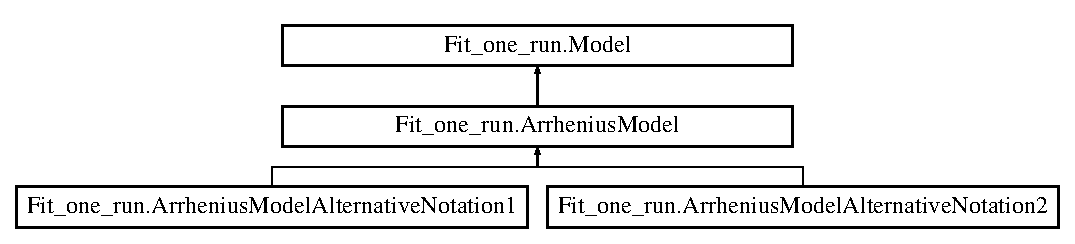
\includegraphics[height=2.828283cm]{classFit__one__run_1_1ArrheniusModel}
\end{center}
\end{figure}
\subsection*{\-Public \-Member \-Functions}
\begin{DoxyCompactItemize}
\item 
\hypertarget{classFit__one__run_1_1ArrheniusModel_ac9a94d1c646a3f830eabced4d3a07ce0}{def {\bfseries \-\_\-\-\_\-init\-\_\-\-\_\-}}\label{classFit__one__run_1_1ArrheniusModel_ac9a94d1c646a3f830eabced4d3a07ce0}

\item 
def \hyperlink{classFit__one__run_1_1ArrheniusModel_aef95e08280a5f8628b63ea1300227aa7}{calc\-Mass}
\item 
def \hyperlink{classFit__one__run_1_1ArrheniusModel_a2d145de8ceef61b26b3ab701618ebb9d}{\-Convert\-Kin\-Factors}
\item 
def \hyperlink{classFit__one__run_1_1Model_aa304b32155938a713c33f0dc03a135f3}{plt\-Yield}
\item 
def \hyperlink{classFit__one__run_1_1Model_a9c28d95902adf00f5aaa642f0919fc61}{plt\-Rate}
\item 
def \hyperlink{classFit__one__run_1_1Model_a26fc879ca33c9171ebb4a97bc4b0c46b}{min\-Length\-Of\-Vectors}
\item 
def \hyperlink{classFit__one__run_1_1Model_a98159c954f1f1be2a34be3ea53d11493}{plot}
\item 
def \hyperlink{classFit__one__run_1_1Model_ace9df4177c5ae753dbe190e2f8268149}{derive\-C}
\item 
def \hyperlink{classFit__one__run_1_1Model_a07ae4534de2a6ef241d71facdffb227e}{calc\-Rate}
\item 
def \hyperlink{classFit__one__run_1_1Model_a174aec9b05dbe01ec103f7ba75d6516c}{set\-Param\-Vector}
\item 
def \hyperlink{classFit__one__run_1_1Model_a3c9239f0ac062fdae0bda395636c0372}{\-Param\-Vector}
\item 
def \hyperlink{classFit__one__run_1_1Model_aa2bc4ba19704350fb2ff441734b51b10}{\-Error\-Yield}
\item 
def \hyperlink{classFit__one__run_1_1Model_aad63c345c343f0c7d1cf20135dc0a0e5}{\-Error\-Rate}
\end{DoxyCompactItemize}
\subsection*{\-Public \-Attributes}
\begin{DoxyCompactItemize}
\item 
\hypertarget{classFit__one__run_1_1ArrheniusModel_aed77ff30b973e7ff77113c19c4ba78fa}{{\bfseries \-O\-D\-E\-\_\-hmax}}\label{classFit__one__run_1_1ArrheniusModel_aed77ff30b973e7ff77113c19c4ba78fa}

\end{DoxyCompactItemize}


\subsection{\-Detailed \-Description}
\begin{DoxyVerb}The Arrhenius model in the standart notation: dm/dt=A*(T**b)*exp(-E/T)*(m_s-m) with the parameter a,b,E to optimize.\end{DoxyVerb}
 

\subsection{\-Member \-Function \-Documentation}
\hypertarget{classFit__one__run_1_1ArrheniusModel_aef95e08280a5f8628b63ea1300227aa7}{\index{\-Fit\-\_\-one\-\_\-run\-::\-Arrhenius\-Model@{\-Fit\-\_\-one\-\_\-run\-::\-Arrhenius\-Model}!calc\-Mass@{calc\-Mass}}
\index{calc\-Mass@{calc\-Mass}!Fit_one_run::ArrheniusModel@{\-Fit\-\_\-one\-\_\-run\-::\-Arrhenius\-Model}}
\subsubsection[{calc\-Mass}]{\setlength{\rightskip}{0pt plus 5cm}def {\bf \-Fit\-\_\-one\-\_\-run.\-Arrhenius\-Model.\-calc\-Mass} (
\begin{DoxyParamCaption}
\item[{}]{self, }
\item[{}]{fgdvc, }
\item[{}]{time, }
\item[{}]{\-T, }
\item[{}]{\-Name}
\end{DoxyParamCaption}
)}}\label{classFit__one__run_1_1ArrheniusModel_aef95e08280a5f8628b63ea1300227aa7}
\begin{DoxyVerb}Outputs the mass(t) using the model specific equation.\end{DoxyVerb}
 

\-Reimplemented in \hyperlink{classFit__one__run_1_1ArrheniusModelAlternativeNotation2_ad2b7981d11c82b7fb90f476396655f3f}{\-Fit\-\_\-one\-\_\-run.\-Arrhenius\-Model\-Alternative\-Notation2}, and \hyperlink{classFit__one__run_1_1ArrheniusModelAlternativeNotation1_ae5173ca0b3b89ddf7d5407a6023d693f}{\-Fit\-\_\-one\-\_\-run.\-Arrhenius\-Model\-Alternative\-Notation1}.

\hypertarget{classFit__one__run_1_1Model_a07ae4534de2a6ef241d71facdffb227e}{\index{\-Fit\-\_\-one\-\_\-run\-::\-Arrhenius\-Model@{\-Fit\-\_\-one\-\_\-run\-::\-Arrhenius\-Model}!calc\-Rate@{calc\-Rate}}
\index{calc\-Rate@{calc\-Rate}!Fit_one_run::ArrheniusModel@{\-Fit\-\_\-one\-\_\-run\-::\-Arrhenius\-Model}}
\subsubsection[{calc\-Rate}]{\setlength{\rightskip}{0pt plus 5cm}def {\bf \-Fit\-\_\-one\-\_\-run.\-Model.\-calc\-Rate} (
\begin{DoxyParamCaption}
\item[{}]{self, }
\item[{}]{fgdvc, }
\item[{}]{time, }
\item[{}]{\-T, }
\item[{}]{\-Name}
\end{DoxyParamCaption}
)\hspace{0.3cm}{\ttfamily  \mbox{[}inherited\mbox{]}}}}\label{classFit__one__run_1_1Model_a07ae4534de2a6ef241d71facdffb227e}
\begin{DoxyVerb}Generates the Rates using the yields vector and a CDS.\end{DoxyVerb}
 \hypertarget{classFit__one__run_1_1ArrheniusModel_a2d145de8ceef61b26b3ab701618ebb9d}{\index{\-Fit\-\_\-one\-\_\-run\-::\-Arrhenius\-Model@{\-Fit\-\_\-one\-\_\-run\-::\-Arrhenius\-Model}!\-Convert\-Kin\-Factors@{\-Convert\-Kin\-Factors}}
\index{\-Convert\-Kin\-Factors@{\-Convert\-Kin\-Factors}!Fit_one_run::ArrheniusModel@{\-Fit\-\_\-one\-\_\-run\-::\-Arrhenius\-Model}}
\subsubsection[{\-Convert\-Kin\-Factors}]{\setlength{\rightskip}{0pt plus 5cm}def {\bf \-Fit\-\_\-one\-\_\-run.\-Arrhenius\-Model.\-Convert\-Kin\-Factors} (
\begin{DoxyParamCaption}
\item[{}]{self, }
\item[{}]{\-Parameter\-Vector}
\end{DoxyParamCaption}
)}}\label{classFit__one__run_1_1ArrheniusModel_a2d145de8ceef61b26b3ab701618ebb9d}
\begin{DoxyVerb}Dummy. Function actual has to convert the parameter into the standart Arrhenius notation.\end{DoxyVerb}
 

\-Reimplemented in \hyperlink{classFit__one__run_1_1ArrheniusModelAlternativeNotation2_a4f6e2eb68a60c1dbdbb6176ad7cf508a}{\-Fit\-\_\-one\-\_\-run.\-Arrhenius\-Model\-Alternative\-Notation2}, and \hyperlink{classFit__one__run_1_1ArrheniusModelAlternativeNotation1_a0bec2d240a20bdd5b5e4a08bf603c705}{\-Fit\-\_\-one\-\_\-run.\-Arrhenius\-Model\-Alternative\-Notation1}.

\hypertarget{classFit__one__run_1_1Model_ace9df4177c5ae753dbe190e2f8268149}{\index{\-Fit\-\_\-one\-\_\-run\-::\-Arrhenius\-Model@{\-Fit\-\_\-one\-\_\-run\-::\-Arrhenius\-Model}!derive\-C@{derive\-C}}
\index{derive\-C@{derive\-C}!Fit_one_run::ArrheniusModel@{\-Fit\-\_\-one\-\_\-run\-::\-Arrhenius\-Model}}
\subsubsection[{derive\-C}]{\setlength{\rightskip}{0pt plus 5cm}def {\bf \-Fit\-\_\-one\-\_\-run.\-Model.\-derive\-C} (
\begin{DoxyParamCaption}
\item[{}]{self, }
\item[{}]{fgdvc, }
\item[{}]{y\-Vector, }
\item[{}]{max\-Vector\-Lenght = {\ttfamily \-None}}
\end{DoxyParamCaption}
)\hspace{0.3cm}{\ttfamily  \mbox{[}inherited\mbox{]}}}}\label{classFit__one__run_1_1Model_ace9df4177c5ae753dbe190e2f8268149}
\begin{DoxyVerb}Returns a CDS of the inputted yVector.\end{DoxyVerb}
 \hypertarget{classFit__one__run_1_1Model_aad63c345c343f0c7d1cf20135dc0a0e5}{\index{\-Fit\-\_\-one\-\_\-run\-::\-Arrhenius\-Model@{\-Fit\-\_\-one\-\_\-run\-::\-Arrhenius\-Model}!\-Error\-Rate@{\-Error\-Rate}}
\index{\-Error\-Rate@{\-Error\-Rate}!Fit_one_run::ArrheniusModel@{\-Fit\-\_\-one\-\_\-run\-::\-Arrhenius\-Model}}
\subsubsection[{\-Error\-Rate}]{\setlength{\rightskip}{0pt plus 5cm}def {\bf \-Fit\-\_\-one\-\_\-run.\-Model.\-Error\-Rate} (
\begin{DoxyParamCaption}
\item[{}]{self, }
\item[{}]{fgdvc, }
\item[{}]{\-Species}
\end{DoxyParamCaption}
)\hspace{0.3cm}{\ttfamily  \mbox{[}inherited\mbox{]}}}}\label{classFit__one__run_1_1Model_aad63c345c343f0c7d1cf20135dc0a0e5}
\begin{DoxyVerb}Returns the absolute deviation per point between the fitted and the original rate curve.\end{DoxyVerb}
 \hypertarget{classFit__one__run_1_1Model_aa2bc4ba19704350fb2ff441734b51b10}{\index{\-Fit\-\_\-one\-\_\-run\-::\-Arrhenius\-Model@{\-Fit\-\_\-one\-\_\-run\-::\-Arrhenius\-Model}!\-Error\-Yield@{\-Error\-Yield}}
\index{\-Error\-Yield@{\-Error\-Yield}!Fit_one_run::ArrheniusModel@{\-Fit\-\_\-one\-\_\-run\-::\-Arrhenius\-Model}}
\subsubsection[{\-Error\-Yield}]{\setlength{\rightskip}{0pt plus 5cm}def {\bf \-Fit\-\_\-one\-\_\-run.\-Model.\-Error\-Yield} (
\begin{DoxyParamCaption}
\item[{}]{self, }
\item[{}]{fgdvc, }
\item[{}]{\-Species}
\end{DoxyParamCaption}
)\hspace{0.3cm}{\ttfamily  \mbox{[}inherited\mbox{]}}}}\label{classFit__one__run_1_1Model_aa2bc4ba19704350fb2ff441734b51b10}
\begin{DoxyVerb}Returns the absolute deviation per point between the fitted and the original yield curve.\end{DoxyVerb}
 \hypertarget{classFit__one__run_1_1Model_a26fc879ca33c9171ebb4a97bc4b0c46b}{\index{\-Fit\-\_\-one\-\_\-run\-::\-Arrhenius\-Model@{\-Fit\-\_\-one\-\_\-run\-::\-Arrhenius\-Model}!min\-Length\-Of\-Vectors@{min\-Length\-Of\-Vectors}}
\index{min\-Length\-Of\-Vectors@{min\-Length\-Of\-Vectors}!Fit_one_run::ArrheniusModel@{\-Fit\-\_\-one\-\_\-run\-::\-Arrhenius\-Model}}
\subsubsection[{min\-Length\-Of\-Vectors}]{\setlength{\rightskip}{0pt plus 5cm}def {\bf \-Fit\-\_\-one\-\_\-run.\-Model.\-min\-Length\-Of\-Vectors} (
\begin{DoxyParamCaption}
\item[{}]{self, }
\item[{}]{fgdvc\-\_\-list}
\end{DoxyParamCaption}
)\hspace{0.3cm}{\ttfamily  \mbox{[}inherited\mbox{]}}}}\label{classFit__one__run_1_1Model_a26fc879ca33c9171ebb4a97bc4b0c46b}
\begin{DoxyVerb}Returns the minimum lenght of a all vectors from the several runs.\end{DoxyVerb}
 \hypertarget{classFit__one__run_1_1Model_a3c9239f0ac062fdae0bda395636c0372}{\index{\-Fit\-\_\-one\-\_\-run\-::\-Arrhenius\-Model@{\-Fit\-\_\-one\-\_\-run\-::\-Arrhenius\-Model}!\-Param\-Vector@{\-Param\-Vector}}
\index{\-Param\-Vector@{\-Param\-Vector}!Fit_one_run::ArrheniusModel@{\-Fit\-\_\-one\-\_\-run\-::\-Arrhenius\-Model}}
\subsubsection[{\-Param\-Vector}]{\setlength{\rightskip}{0pt plus 5cm}def {\bf \-Fit\-\_\-one\-\_\-run.\-Model.\-Param\-Vector} (
\begin{DoxyParamCaption}
\item[{}]{self}
\end{DoxyParamCaption}
)\hspace{0.3cm}{\ttfamily  \mbox{[}inherited\mbox{]}}}}\label{classFit__one__run_1_1Model_a3c9239f0ac062fdae0bda395636c0372}
\begin{DoxyVerb}Returns the Vector containing the kinetic parameter of the Model (refering to the child model).\end{DoxyVerb}
 \hypertarget{classFit__one__run_1_1Model_a98159c954f1f1be2a34be3ea53d11493}{\index{\-Fit\-\_\-one\-\_\-run\-::\-Arrhenius\-Model@{\-Fit\-\_\-one\-\_\-run\-::\-Arrhenius\-Model}!plot@{plot}}
\index{plot@{plot}!Fit_one_run::ArrheniusModel@{\-Fit\-\_\-one\-\_\-run\-::\-Arrhenius\-Model}}
\subsubsection[{plot}]{\setlength{\rightskip}{0pt plus 5cm}def {\bf \-Fit\-\_\-one\-\_\-run.\-Model.\-plot} (
\begin{DoxyParamCaption}
\item[{}]{self, }
\item[{}]{fgdvc\-\_\-list, }
\item[{}]{\-Species}
\end{DoxyParamCaption}
)\hspace{0.3cm}{\ttfamily  \mbox{[}inherited\mbox{]}}}}\label{classFit__one__run_1_1Model_a98159c954f1f1be2a34be3ea53d11493}
\begin{DoxyVerb}Plot the yield and the rates over time with two curves: one is the original data, the other the fitting curve. Also file 'PyrolysisProgramName-Species.out' (e.g. 'CPD-CO2.out') containing the time (s), yields (kg/kg), rates (kg/(kg s)).\end{DoxyVerb}
 \hypertarget{classFit__one__run_1_1Model_a9c28d95902adf00f5aaa642f0919fc61}{\index{\-Fit\-\_\-one\-\_\-run\-::\-Arrhenius\-Model@{\-Fit\-\_\-one\-\_\-run\-::\-Arrhenius\-Model}!plt\-Rate@{plt\-Rate}}
\index{plt\-Rate@{plt\-Rate}!Fit_one_run::ArrheniusModel@{\-Fit\-\_\-one\-\_\-run\-::\-Arrhenius\-Model}}
\subsubsection[{plt\-Rate}]{\setlength{\rightskip}{0pt plus 5cm}def {\bf \-Fit\-\_\-one\-\_\-run.\-Model.\-plt\-Rate} (
\begin{DoxyParamCaption}
\item[{}]{self, }
\item[{}]{fgdvc\-\_\-list, }
\item[{}]{x\-Value\-To\-Plot, }
\item[{}]{y\-Value\-To\-Plot}
\end{DoxyParamCaption}
)\hspace{0.3cm}{\ttfamily  \mbox{[}inherited\mbox{]}}}}\label{classFit__one__run_1_1Model_a9c28d95902adf00f5aaa642f0919fc61}
\begin{DoxyVerb}Plots the rates (to select with yValueToPlot) over Time or Temperature (to slect with xValueToPlot).\end{DoxyVerb}
 \hypertarget{classFit__one__run_1_1Model_aa304b32155938a713c33f0dc03a135f3}{\index{\-Fit\-\_\-one\-\_\-run\-::\-Arrhenius\-Model@{\-Fit\-\_\-one\-\_\-run\-::\-Arrhenius\-Model}!plt\-Yield@{plt\-Yield}}
\index{plt\-Yield@{plt\-Yield}!Fit_one_run::ArrheniusModel@{\-Fit\-\_\-one\-\_\-run\-::\-Arrhenius\-Model}}
\subsubsection[{plt\-Yield}]{\setlength{\rightskip}{0pt plus 5cm}def {\bf \-Fit\-\_\-one\-\_\-run.\-Model.\-plt\-Yield} (
\begin{DoxyParamCaption}
\item[{}]{self, }
\item[{}]{fgdvc\-\_\-list, }
\item[{}]{x\-Value\-To\-Plot, }
\item[{}]{y\-Value\-To\-Plot}
\end{DoxyParamCaption}
)\hspace{0.3cm}{\ttfamily  \mbox{[}inherited\mbox{]}}}}\label{classFit__one__run_1_1Model_aa304b32155938a713c33f0dc03a135f3}
\begin{DoxyVerb}Plots the yields (to select with yValueToPlot) over Time or Temperature (to slect with xValueToPlot).\end{DoxyVerb}
 \hypertarget{classFit__one__run_1_1Model_a174aec9b05dbe01ec103f7ba75d6516c}{\index{\-Fit\-\_\-one\-\_\-run\-::\-Arrhenius\-Model@{\-Fit\-\_\-one\-\_\-run\-::\-Arrhenius\-Model}!set\-Param\-Vector@{set\-Param\-Vector}}
\index{set\-Param\-Vector@{set\-Param\-Vector}!Fit_one_run::ArrheniusModel@{\-Fit\-\_\-one\-\_\-run\-::\-Arrhenius\-Model}}
\subsubsection[{set\-Param\-Vector}]{\setlength{\rightskip}{0pt plus 5cm}def {\bf \-Fit\-\_\-one\-\_\-run.\-Model.\-set\-Param\-Vector} (
\begin{DoxyParamCaption}
\item[{}]{self, }
\item[{}]{\-Parameter\-List}
\end{DoxyParamCaption}
)\hspace{0.3cm}{\ttfamily  \mbox{[}inherited\mbox{]}}}}\label{classFit__one__run_1_1Model_a174aec9b05dbe01ec103f7ba75d6516c}
\begin{DoxyVerb}Sets the Vector containing the kinetic parameter of the Model (refering to the child model).\end{DoxyVerb}
 

\-The documentation for this class was generated from the following file\-:\begin{DoxyCompactItemize}
\item 
/home/map/git/pkp/src/\-Fit\-\_\-one\-\_\-run.\-py\end{DoxyCompactItemize}

\hypertarget{classModels_1_1ArrheniusModel}{\section{\-Models.\-Arrhenius\-Model \-Class \-Reference}
\label{classModels_1_1ArrheniusModel}\index{\-Models.\-Arrhenius\-Model@{\-Models.\-Arrhenius\-Model}}
}
\-Inheritance diagram for \-Models.\-Arrhenius\-Model\-:\begin{figure}[H]
\begin{center}
\leavevmode
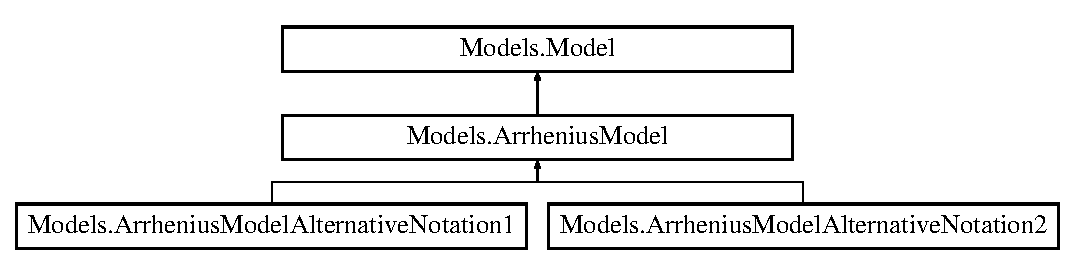
\includegraphics[height=3.000000cm]{classModels_1_1ArrheniusModel}
\end{center}
\end{figure}
\subsection*{\-Public \-Member \-Functions}
\begin{DoxyCompactItemize}
\item 
\hypertarget{classModels_1_1ArrheniusModel_aed66810f882bde4a28b94ef527575b4d}{def {\bfseries \-\_\-\-\_\-init\-\_\-\-\_\-}}\label{classModels_1_1ArrheniusModel_aed66810f882bde4a28b94ef527575b4d}

\item 
def \hyperlink{classModels_1_1ArrheniusModel_abb4fedac573a2f263fd5bb4cd284ce65}{calc\-Mass}
\item 
def \hyperlink{classModels_1_1ArrheniusModel_a946e6177077d67613160aaaedde95faa}{\-Convert\-Kin\-Factors}
\item 
def \hyperlink{classModels_1_1Model_a317ed848b969dbe3a96dd05e8b771900}{plt\-Yield}
\item 
def \hyperlink{classModels_1_1Model_aa35c741babf8f141df48c4021e0664e4}{plt\-Rate}
\item 
def \hyperlink{classModels_1_1Model_a3396d6ca1a7b7d66e55ada8c3c7a509e}{max\-Length\-Of\-Vectors}
\item 
def \hyperlink{classModels_1_1Model_ae404a691e48bfe4eafcdfdd09f1dae48}{plot}
\item 
def \hyperlink{classModels_1_1Model_a010945ed2adff59a7a5fce36025e7a97}{derive\-C}
\item 
def \hyperlink{classModels_1_1Model_a7c9280e33f9e0d46703cebc131008c65}{calc\-Rate}
\item 
def \hyperlink{classModels_1_1Model_a818f207e2a4bd0e9a3720ca611960e5a}{set\-Param\-Vector}
\item 
def \hyperlink{classModels_1_1Model_a13c76a0fe24d43cdc4d21fbc73fa96fa}{\-Param\-Vector}
\item 
def \hyperlink{classModels_1_1Model_ad3e627980d9e781bf7b2c9ff900ca06b}{\-Error\-Yield}
\item 
def \hyperlink{classModels_1_1Model_a3050eb39341f318d8d88b172f88bd240}{\-Error\-Rate}
\item 
def \hyperlink{classModels_1_1Model_adcb987bccae63a742490ea1e6d5f7a74}{mk\-Simple\-Result\-Files}
\item 
def \hyperlink{classModels_1_1Model_ac28252ae5cd6b5ecd4c5d006a0e6567d}{set\-Dt4\-Intergrate}
\end{DoxyCompactItemize}
\subsection*{\-Public \-Attributes}
\begin{DoxyCompactItemize}
\item 
\hypertarget{classModels_1_1ArrheniusModel_ab9b265e22c3b12bcde234f3a79b3f8f8}{{\bfseries \-O\-D\-E\-\_\-hmax}}\label{classModels_1_1ArrheniusModel_ab9b265e22c3b12bcde234f3a79b3f8f8}

\item 
\hypertarget{classModels_1_1ArrheniusModel_a2e2beed5b0008f628f9a9f6bff7aff0d}{{\bfseries const\-Dt}}\label{classModels_1_1ArrheniusModel_a2e2beed5b0008f628f9a9f6bff7aff0d}

\item 
\hypertarget{classModels_1_1Model_a3f71983de5f8b86bec47929213b900ec}{{\bfseries const\-Dt\-Vec}}\label{classModels_1_1Model_a3f71983de5f8b86bec47929213b900ec}

\end{DoxyCompactItemize}


\subsection{\-Detailed \-Description}
\begin{DoxyVerb}The Arrhenius model in the standart notation: dm/dt=A*(T**b)*exp(-E/T)*(m_s-m) with the parameter a,b,E to optimize.\end{DoxyVerb}
 

\subsection{\-Member \-Function \-Documentation}
\hypertarget{classModels_1_1ArrheniusModel_abb4fedac573a2f263fd5bb4cd284ce65}{\index{\-Models\-::\-Arrhenius\-Model@{\-Models\-::\-Arrhenius\-Model}!calc\-Mass@{calc\-Mass}}
\index{calc\-Mass@{calc\-Mass}!Models::ArrheniusModel@{\-Models\-::\-Arrhenius\-Model}}
\subsubsection[{calc\-Mass}]{\setlength{\rightskip}{0pt plus 5cm}def {\bf \-Models.\-Arrhenius\-Model.\-calc\-Mass} (
\begin{DoxyParamCaption}
\item[{}]{self, }
\item[{}]{fgdvc, }
\item[{}]{time, }
\item[{}]{\-T, }
\item[{}]{\-Name}
\end{DoxyParamCaption}
)}}\label{classModels_1_1ArrheniusModel_abb4fedac573a2f263fd5bb4cd284ce65}
\begin{DoxyVerb}Outputs the mass(t) using the model specific equation.\end{DoxyVerb}
 

\-Reimplemented in \hyperlink{classModels_1_1ArrheniusModelAlternativeNotation2_afe70c590fc443e5d91a51485089c513f}{\-Models.\-Arrhenius\-Model\-Alternative\-Notation2}, and \hyperlink{classModels_1_1ArrheniusModelAlternativeNotation1_a977524416ab6b41aa7ca01c844074123}{\-Models.\-Arrhenius\-Model\-Alternative\-Notation1}.

\hypertarget{classModels_1_1Model_a7c9280e33f9e0d46703cebc131008c65}{\index{\-Models\-::\-Arrhenius\-Model@{\-Models\-::\-Arrhenius\-Model}!calc\-Rate@{calc\-Rate}}
\index{calc\-Rate@{calc\-Rate}!Models::ArrheniusModel@{\-Models\-::\-Arrhenius\-Model}}
\subsubsection[{calc\-Rate}]{\setlength{\rightskip}{0pt plus 5cm}def {\bf \-Models.\-Model.\-calc\-Rate} (
\begin{DoxyParamCaption}
\item[{}]{self, }
\item[{}]{fgdvc, }
\item[{}]{time, }
\item[{}]{\-T, }
\item[{}]{\-Name}
\end{DoxyParamCaption}
)\hspace{0.3cm}{\ttfamily  \mbox{[}inherited\mbox{]}}}}\label{classModels_1_1Model_a7c9280e33f9e0d46703cebc131008c65}
\begin{DoxyVerb}Generates the Rates using the yields vector and a CDS.\end{DoxyVerb}
 \hypertarget{classModels_1_1ArrheniusModel_a946e6177077d67613160aaaedde95faa}{\index{\-Models\-::\-Arrhenius\-Model@{\-Models\-::\-Arrhenius\-Model}!\-Convert\-Kin\-Factors@{\-Convert\-Kin\-Factors}}
\index{\-Convert\-Kin\-Factors@{\-Convert\-Kin\-Factors}!Models::ArrheniusModel@{\-Models\-::\-Arrhenius\-Model}}
\subsubsection[{\-Convert\-Kin\-Factors}]{\setlength{\rightskip}{0pt plus 5cm}def {\bf \-Models.\-Arrhenius\-Model.\-Convert\-Kin\-Factors} (
\begin{DoxyParamCaption}
\item[{}]{self, }
\item[{}]{\-Parameter\-Vector}
\end{DoxyParamCaption}
)}}\label{classModels_1_1ArrheniusModel_a946e6177077d67613160aaaedde95faa}
\begin{DoxyVerb}Dummy. Function actual has to convert the parameter into the standart Arrhenius notation.\end{DoxyVerb}
 

\-Reimplemented in \hyperlink{classModels_1_1ArrheniusModelAlternativeNotation2_a82aa3ccadb987ed778dde97edaf5b687}{\-Models.\-Arrhenius\-Model\-Alternative\-Notation2}, and \hyperlink{classModels_1_1ArrheniusModelAlternativeNotation1_a81e74ccd401041164b6a9d697e836397}{\-Models.\-Arrhenius\-Model\-Alternative\-Notation1}.

\hypertarget{classModels_1_1Model_a010945ed2adff59a7a5fce36025e7a97}{\index{\-Models\-::\-Arrhenius\-Model@{\-Models\-::\-Arrhenius\-Model}!derive\-C@{derive\-C}}
\index{derive\-C@{derive\-C}!Models::ArrheniusModel@{\-Models\-::\-Arrhenius\-Model}}
\subsubsection[{derive\-C}]{\setlength{\rightskip}{0pt plus 5cm}def {\bf \-Models.\-Model.\-derive\-C} (
\begin{DoxyParamCaption}
\item[{}]{self, }
\item[{}]{fgdvc, }
\item[{}]{y\-Vector}
\end{DoxyParamCaption}
)\hspace{0.3cm}{\ttfamily  \mbox{[}inherited\mbox{]}}}}\label{classModels_1_1Model_a010945ed2adff59a7a5fce36025e7a97}
\begin{DoxyVerb}Returns a CDS of the inputted yVector.\end{DoxyVerb}
 \hypertarget{classModels_1_1Model_a3050eb39341f318d8d88b172f88bd240}{\index{\-Models\-::\-Arrhenius\-Model@{\-Models\-::\-Arrhenius\-Model}!\-Error\-Rate@{\-Error\-Rate}}
\index{\-Error\-Rate@{\-Error\-Rate}!Models::ArrheniusModel@{\-Models\-::\-Arrhenius\-Model}}
\subsubsection[{\-Error\-Rate}]{\setlength{\rightskip}{0pt plus 5cm}def {\bf \-Models.\-Model.\-Error\-Rate} (
\begin{DoxyParamCaption}
\item[{}]{self, }
\item[{}]{fgdvc, }
\item[{}]{\-Species}
\end{DoxyParamCaption}
)\hspace{0.3cm}{\ttfamily  \mbox{[}inherited\mbox{]}}}}\label{classModels_1_1Model_a3050eb39341f318d8d88b172f88bd240}
\begin{DoxyVerb}Returns the absolute deviation per point between the fitted and the original rate curve.\end{DoxyVerb}
 \hypertarget{classModels_1_1Model_ad3e627980d9e781bf7b2c9ff900ca06b}{\index{\-Models\-::\-Arrhenius\-Model@{\-Models\-::\-Arrhenius\-Model}!\-Error\-Yield@{\-Error\-Yield}}
\index{\-Error\-Yield@{\-Error\-Yield}!Models::ArrheniusModel@{\-Models\-::\-Arrhenius\-Model}}
\subsubsection[{\-Error\-Yield}]{\setlength{\rightskip}{0pt plus 5cm}def {\bf \-Models.\-Model.\-Error\-Yield} (
\begin{DoxyParamCaption}
\item[{}]{self, }
\item[{}]{fgdvc, }
\item[{}]{\-Species}
\end{DoxyParamCaption}
)\hspace{0.3cm}{\ttfamily  \mbox{[}inherited\mbox{]}}}}\label{classModels_1_1Model_ad3e627980d9e781bf7b2c9ff900ca06b}
\begin{DoxyVerb}Returns the absolute deviation per point between the fitted and the original yield curve.\end{DoxyVerb}
 \hypertarget{classModels_1_1Model_a3396d6ca1a7b7d66e55ada8c3c7a509e}{\index{\-Models\-::\-Arrhenius\-Model@{\-Models\-::\-Arrhenius\-Model}!max\-Length\-Of\-Vectors@{max\-Length\-Of\-Vectors}}
\index{max\-Length\-Of\-Vectors@{max\-Length\-Of\-Vectors}!Models::ArrheniusModel@{\-Models\-::\-Arrhenius\-Model}}
\subsubsection[{max\-Length\-Of\-Vectors}]{\setlength{\rightskip}{0pt plus 5cm}def {\bf \-Models.\-Model.\-max\-Length\-Of\-Vectors} (
\begin{DoxyParamCaption}
\item[{}]{self, }
\item[{}]{fgdvc\-\_\-list}
\end{DoxyParamCaption}
)\hspace{0.3cm}{\ttfamily  \mbox{[}inherited\mbox{]}}}}\label{classModels_1_1Model_a3396d6ca1a7b7d66e55ada8c3c7a509e}
\begin{DoxyVerb}Returns the minimum lenght of a all vectors from the several runs.\end{DoxyVerb}
 \hypertarget{classModels_1_1Model_adcb987bccae63a742490ea1e6d5f7a74}{\index{\-Models\-::\-Arrhenius\-Model@{\-Models\-::\-Arrhenius\-Model}!mk\-Simple\-Result\-Files@{mk\-Simple\-Result\-Files}}
\index{mk\-Simple\-Result\-Files@{mk\-Simple\-Result\-Files}!Models::ArrheniusModel@{\-Models\-::\-Arrhenius\-Model}}
\subsubsection[{mk\-Simple\-Result\-Files}]{\setlength{\rightskip}{0pt plus 5cm}def {\bf \-Models.\-Model.\-mk\-Simple\-Result\-Files} (
\begin{DoxyParamCaption}
\item[{}]{self, }
\item[{}]{fgdvc\-\_\-list, }
\item[{}]{\-Species}
\end{DoxyParamCaption}
)\hspace{0.3cm}{\ttfamily  \mbox{[}inherited\mbox{]}}}}\label{classModels_1_1Model_adcb987bccae63a742490ea1e6d5f7a74}
\begin{DoxyVerb}Simple result file if no fitting is carried out. Writes only the transformed results into a file.\end{DoxyVerb}
 \hypertarget{classModels_1_1Model_a13c76a0fe24d43cdc4d21fbc73fa96fa}{\index{\-Models\-::\-Arrhenius\-Model@{\-Models\-::\-Arrhenius\-Model}!\-Param\-Vector@{\-Param\-Vector}}
\index{\-Param\-Vector@{\-Param\-Vector}!Models::ArrheniusModel@{\-Models\-::\-Arrhenius\-Model}}
\subsubsection[{\-Param\-Vector}]{\setlength{\rightskip}{0pt plus 5cm}def {\bf \-Models.\-Model.\-Param\-Vector} (
\begin{DoxyParamCaption}
\item[{}]{self}
\end{DoxyParamCaption}
)\hspace{0.3cm}{\ttfamily  \mbox{[}inherited\mbox{]}}}}\label{classModels_1_1Model_a13c76a0fe24d43cdc4d21fbc73fa96fa}
\begin{DoxyVerb}Returns the Vector containing the kinetic parameter of the Model (refering to the child model).\end{DoxyVerb}
 \hypertarget{classModels_1_1Model_ae404a691e48bfe4eafcdfdd09f1dae48}{\index{\-Models\-::\-Arrhenius\-Model@{\-Models\-::\-Arrhenius\-Model}!plot@{plot}}
\index{plot@{plot}!Models::ArrheniusModel@{\-Models\-::\-Arrhenius\-Model}}
\subsubsection[{plot}]{\setlength{\rightskip}{0pt plus 5cm}def {\bf \-Models.\-Model.\-plot} (
\begin{DoxyParamCaption}
\item[{}]{self, }
\item[{}]{fgdvc\-\_\-list, }
\item[{}]{\-Species}
\end{DoxyParamCaption}
)\hspace{0.3cm}{\ttfamily  \mbox{[}inherited\mbox{]}}}}\label{classModels_1_1Model_ae404a691e48bfe4eafcdfdd09f1dae48}
\begin{DoxyVerb}Plot the yield and the rates over time with two curves: one is the original data, the other the fitting curve. Also file 'PyrolysisProgramName-Species.out' (e.g. 'CPD-CO2.out') containing the time (s), yields (kg/kg), rates (kg/(kg s)).\end{DoxyVerb}
 \hypertarget{classModels_1_1Model_aa35c741babf8f141df48c4021e0664e4}{\index{\-Models\-::\-Arrhenius\-Model@{\-Models\-::\-Arrhenius\-Model}!plt\-Rate@{plt\-Rate}}
\index{plt\-Rate@{plt\-Rate}!Models::ArrheniusModel@{\-Models\-::\-Arrhenius\-Model}}
\subsubsection[{plt\-Rate}]{\setlength{\rightskip}{0pt plus 5cm}def {\bf \-Models.\-Model.\-plt\-Rate} (
\begin{DoxyParamCaption}
\item[{}]{self, }
\item[{}]{fgdvc\-\_\-list, }
\item[{}]{x\-Value\-To\-Plot, }
\item[{}]{y\-Value\-To\-Plot}
\end{DoxyParamCaption}
)\hspace{0.3cm}{\ttfamily  \mbox{[}inherited\mbox{]}}}}\label{classModels_1_1Model_aa35c741babf8f141df48c4021e0664e4}
\begin{DoxyVerb}Plots the rates (to select with yValueToPlot) over Time or Temperature (to slect with xValueToPlot).\end{DoxyVerb}
 \hypertarget{classModels_1_1Model_a317ed848b969dbe3a96dd05e8b771900}{\index{\-Models\-::\-Arrhenius\-Model@{\-Models\-::\-Arrhenius\-Model}!plt\-Yield@{plt\-Yield}}
\index{plt\-Yield@{plt\-Yield}!Models::ArrheniusModel@{\-Models\-::\-Arrhenius\-Model}}
\subsubsection[{plt\-Yield}]{\setlength{\rightskip}{0pt plus 5cm}def {\bf \-Models.\-Model.\-plt\-Yield} (
\begin{DoxyParamCaption}
\item[{}]{self, }
\item[{}]{fgdvc\-\_\-list, }
\item[{}]{x\-Value\-To\-Plot, }
\item[{}]{y\-Value\-To\-Plot}
\end{DoxyParamCaption}
)\hspace{0.3cm}{\ttfamily  \mbox{[}inherited\mbox{]}}}}\label{classModels_1_1Model_a317ed848b969dbe3a96dd05e8b771900}
\begin{DoxyVerb}Plots the yields (to select with yValueToPlot) over Time or Temperature (to slect with xValueToPlot).\end{DoxyVerb}
 \hypertarget{classModels_1_1Model_ac28252ae5cd6b5ecd4c5d006a0e6567d}{\index{\-Models\-::\-Arrhenius\-Model@{\-Models\-::\-Arrhenius\-Model}!set\-Dt4\-Intergrate@{set\-Dt4\-Intergrate}}
\index{set\-Dt4\-Intergrate@{set\-Dt4\-Intergrate}!Models::ArrheniusModel@{\-Models\-::\-Arrhenius\-Model}}
\subsubsection[{set\-Dt4\-Intergrate}]{\setlength{\rightskip}{0pt plus 5cm}def {\bf \-Models.\-Model.\-set\-Dt4\-Intergrate} (
\begin{DoxyParamCaption}
\item[{}]{self, }
\item[{}]{constant\-Dt}
\end{DoxyParamCaption}
)\hspace{0.3cm}{\ttfamily  \mbox{[}inherited\mbox{]}}}}\label{classModels_1_1Model_ac28252ae5cd6b5ecd4c5d006a0e6567d}
\begin{DoxyVerb}constantDt allows the option to define numerical time step to solve the ODE. The outputted results ever equal the imported time list (when applying method calcMass Time = [t0,t1,t2,t3,t4]. If these time steps are too large, then is this defined dt used to solve the ODE and the results are linear interploated that way that they correspond to the imported time vector. To reset it, just set constantDt to False.\end{DoxyVerb}
 \hypertarget{classModels_1_1Model_a818f207e2a4bd0e9a3720ca611960e5a}{\index{\-Models\-::\-Arrhenius\-Model@{\-Models\-::\-Arrhenius\-Model}!set\-Param\-Vector@{set\-Param\-Vector}}
\index{set\-Param\-Vector@{set\-Param\-Vector}!Models::ArrheniusModel@{\-Models\-::\-Arrhenius\-Model}}
\subsubsection[{set\-Param\-Vector}]{\setlength{\rightskip}{0pt plus 5cm}def {\bf \-Models.\-Model.\-set\-Param\-Vector} (
\begin{DoxyParamCaption}
\item[{}]{self, }
\item[{}]{\-Parameter\-List}
\end{DoxyParamCaption}
)\hspace{0.3cm}{\ttfamily  \mbox{[}inherited\mbox{]}}}}\label{classModels_1_1Model_a818f207e2a4bd0e9a3720ca611960e5a}
\begin{DoxyVerb}Sets the Vector containing the kinetic parameter of the Model (refering to the child model).\end{DoxyVerb}
 

\-The documentation for this class was generated from the following file\-:\begin{DoxyCompactItemize}
\item 
/home/map/git/pkp/src/\-Models.\-py\end{DoxyCompactItemize}

\hypertarget{classModels_1_1ArrheniusModelAlternativeNotation1}{\section{\-Models.\-Arrhenius\-Model\-Alternative\-Notation1 \-Class \-Reference}
\label{classModels_1_1ArrheniusModelAlternativeNotation1}\index{\-Models.\-Arrhenius\-Model\-Alternative\-Notation1@{\-Models.\-Arrhenius\-Model\-Alternative\-Notation1}}
}
\-Inheritance diagram for \-Models.\-Arrhenius\-Model\-Alternative\-Notation1\-:\begin{figure}[H]
\begin{center}
\leavevmode
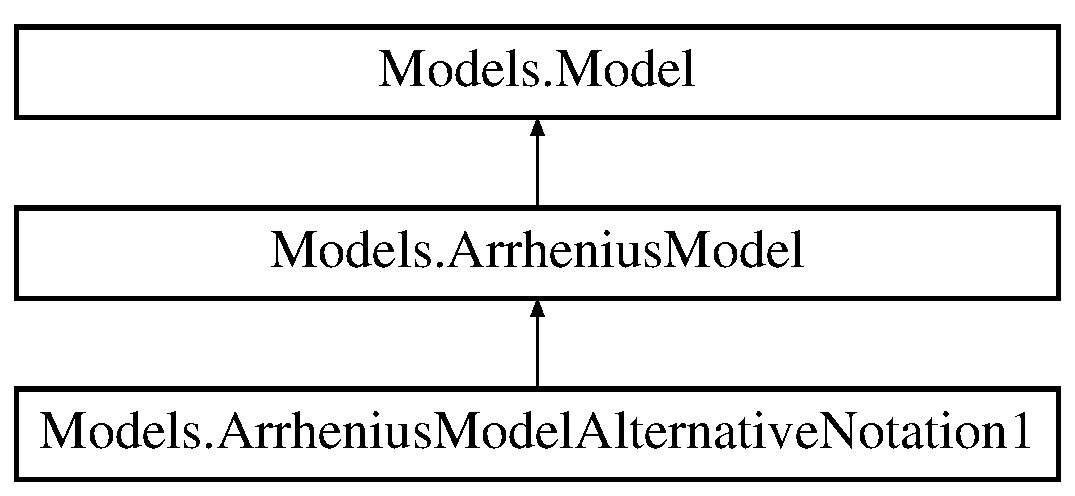
\includegraphics[height=3.000000cm]{classModels_1_1ArrheniusModelAlternativeNotation1}
\end{center}
\end{figure}
\subsection*{\-Public \-Member \-Functions}
\begin{DoxyCompactItemize}
\item 
\hypertarget{classModels_1_1ArrheniusModelAlternativeNotation1_ab492f16aad89e9c4a5bee8b2034c10c1}{def {\bfseries \-\_\-\-\_\-init\-\_\-\-\_\-}}\label{classModels_1_1ArrheniusModelAlternativeNotation1_ab492f16aad89e9c4a5bee8b2034c10c1}

\item 
def \hyperlink{classModels_1_1ArrheniusModelAlternativeNotation1_a977524416ab6b41aa7ca01c844074123}{calc\-Mass}
\item 
def \hyperlink{classModels_1_1ArrheniusModelAlternativeNotation1_a81e74ccd401041164b6a9d697e836397}{\-Convert\-Kin\-Factors}
\item 
def \hyperlink{classModels_1_1ArrheniusModelAlternativeNotation1_a2f46b8d8a2f59735e2053a85bc18fec9}{\-Convert\-Kin\-Factors\-To\-Own\-Notation}
\item 
def \hyperlink{classModels_1_1Model_a317ed848b969dbe3a96dd05e8b771900}{plt\-Yield}
\item 
def \hyperlink{classModels_1_1Model_aa35c741babf8f141df48c4021e0664e4}{plt\-Rate}
\item 
def \hyperlink{classModels_1_1Model_a3396d6ca1a7b7d66e55ada8c3c7a509e}{max\-Length\-Of\-Vectors}
\item 
def \hyperlink{classModels_1_1Model_ae404a691e48bfe4eafcdfdd09f1dae48}{plot}
\item 
def \hyperlink{classModels_1_1Model_a010945ed2adff59a7a5fce36025e7a97}{derive\-C}
\item 
def \hyperlink{classModels_1_1Model_a7c9280e33f9e0d46703cebc131008c65}{calc\-Rate}
\item 
def \hyperlink{classModels_1_1Model_a818f207e2a4bd0e9a3720ca611960e5a}{set\-Param\-Vector}
\item 
def \hyperlink{classModels_1_1Model_a13c76a0fe24d43cdc4d21fbc73fa96fa}{\-Param\-Vector}
\item 
def \hyperlink{classModels_1_1Model_ad3e627980d9e781bf7b2c9ff900ca06b}{\-Error\-Yield}
\item 
def \hyperlink{classModels_1_1Model_a3050eb39341f318d8d88b172f88bd240}{\-Error\-Rate}
\item 
def \hyperlink{classModels_1_1Model_adcb987bccae63a742490ea1e6d5f7a74}{mk\-Simple\-Result\-Files}
\item 
def \hyperlink{classModels_1_1Model_ac28252ae5cd6b5ecd4c5d006a0e6567d}{set\-Dt4\-Intergrate}
\end{DoxyCompactItemize}
\subsection*{\-Public \-Attributes}
\begin{DoxyCompactItemize}
\item 
\hypertarget{classModels_1_1ArrheniusModelAlternativeNotation1_ab8132192339934ceea7d1648bd34b32b}{{\bfseries \-O\-D\-E\-\_\-hmax}}\label{classModels_1_1ArrheniusModelAlternativeNotation1_ab8132192339934ceea7d1648bd34b32b}

\item 
\hypertarget{classModels_1_1ArrheniusModelAlternativeNotation1_abe5a4fb1d1b0647b9f0b2d6e0d97847a}{{\bfseries const\-Dt}}\label{classModels_1_1ArrheniusModelAlternativeNotation1_abe5a4fb1d1b0647b9f0b2d6e0d97847a}

\item 
\hypertarget{classModels_1_1ArrheniusModelAlternativeNotation1_a2bd7e9b3e4a167201e2634b5c7865255}{{\bfseries \-T0}}\label{classModels_1_1ArrheniusModelAlternativeNotation1_a2bd7e9b3e4a167201e2634b5c7865255}

\item 
\hypertarget{classModels_1_1Model_a3f71983de5f8b86bec47929213b900ec}{{\bfseries const\-Dt\-Vec}}\label{classModels_1_1Model_a3f71983de5f8b86bec47929213b900ec}

\end{DoxyCompactItemize}


\subsection{\-Detailed \-Description}
\begin{DoxyVerb}Arrhenius model with a notation having a better optimization behaviour: dm/dt=exp[k0-a*(T0/T(t)-1)]*(ms-m). See the documentation for the reference. The parameters to optimize are k0 and a.\end{DoxyVerb}
 

\subsection{\-Member \-Function \-Documentation}
\hypertarget{classModels_1_1ArrheniusModelAlternativeNotation1_a977524416ab6b41aa7ca01c844074123}{\index{\-Models\-::\-Arrhenius\-Model\-Alternative\-Notation1@{\-Models\-::\-Arrhenius\-Model\-Alternative\-Notation1}!calc\-Mass@{calc\-Mass}}
\index{calc\-Mass@{calc\-Mass}!Models::ArrheniusModelAlternativeNotation1@{\-Models\-::\-Arrhenius\-Model\-Alternative\-Notation1}}
\subsubsection[{calc\-Mass}]{\setlength{\rightskip}{0pt plus 5cm}def {\bf \-Models.\-Arrhenius\-Model\-Alternative\-Notation1.\-calc\-Mass} (
\begin{DoxyParamCaption}
\item[{}]{self, }
\item[{}]{fgdvc, }
\item[{}]{time, }
\item[{}]{\-T, }
\item[{}]{\-Name}
\end{DoxyParamCaption}
)}}\label{classModels_1_1ArrheniusModelAlternativeNotation1_a977524416ab6b41aa7ca01c844074123}
\begin{DoxyVerb}Outputs the mass(t) using the model specific equation.\end{DoxyVerb}
 

\-Reimplemented from \hyperlink{classModels_1_1ArrheniusModel_abb4fedac573a2f263fd5bb4cd284ce65}{\-Models.\-Arrhenius\-Model}.

\hypertarget{classModels_1_1Model_a7c9280e33f9e0d46703cebc131008c65}{\index{\-Models\-::\-Arrhenius\-Model\-Alternative\-Notation1@{\-Models\-::\-Arrhenius\-Model\-Alternative\-Notation1}!calc\-Rate@{calc\-Rate}}
\index{calc\-Rate@{calc\-Rate}!Models::ArrheniusModelAlternativeNotation1@{\-Models\-::\-Arrhenius\-Model\-Alternative\-Notation1}}
\subsubsection[{calc\-Rate}]{\setlength{\rightskip}{0pt plus 5cm}def {\bf \-Models.\-Model.\-calc\-Rate} (
\begin{DoxyParamCaption}
\item[{}]{self, }
\item[{}]{fgdvc, }
\item[{}]{time, }
\item[{}]{\-T, }
\item[{}]{\-Name}
\end{DoxyParamCaption}
)\hspace{0.3cm}{\ttfamily  \mbox{[}inherited\mbox{]}}}}\label{classModels_1_1Model_a7c9280e33f9e0d46703cebc131008c65}
\begin{DoxyVerb}Generates the Rates using the yields vector and a CDS.\end{DoxyVerb}
 \hypertarget{classModels_1_1ArrheniusModelAlternativeNotation1_a81e74ccd401041164b6a9d697e836397}{\index{\-Models\-::\-Arrhenius\-Model\-Alternative\-Notation1@{\-Models\-::\-Arrhenius\-Model\-Alternative\-Notation1}!\-Convert\-Kin\-Factors@{\-Convert\-Kin\-Factors}}
\index{\-Convert\-Kin\-Factors@{\-Convert\-Kin\-Factors}!Models::ArrheniusModelAlternativeNotation1@{\-Models\-::\-Arrhenius\-Model\-Alternative\-Notation1}}
\subsubsection[{\-Convert\-Kin\-Factors}]{\setlength{\rightskip}{0pt plus 5cm}def {\bf \-Models.\-Arrhenius\-Model\-Alternative\-Notation1.\-Convert\-Kin\-Factors} (
\begin{DoxyParamCaption}
\item[{}]{self, }
\item[{}]{\-Parameter\-Vector}
\end{DoxyParamCaption}
)}}\label{classModels_1_1ArrheniusModelAlternativeNotation1_a81e74ccd401041164b6a9d697e836397}
\begin{DoxyVerb}Converts the own kinetic factors back to the standard Arrhenius kinetic factors.\end{DoxyVerb}
 

\-Reimplemented from \hyperlink{classModels_1_1ArrheniusModel_a946e6177077d67613160aaaedde95faa}{\-Models.\-Arrhenius\-Model}.

\hypertarget{classModels_1_1ArrheniusModelAlternativeNotation1_a2f46b8d8a2f59735e2053a85bc18fec9}{\index{\-Models\-::\-Arrhenius\-Model\-Alternative\-Notation1@{\-Models\-::\-Arrhenius\-Model\-Alternative\-Notation1}!\-Convert\-Kin\-Factors\-To\-Own\-Notation@{\-Convert\-Kin\-Factors\-To\-Own\-Notation}}
\index{\-Convert\-Kin\-Factors\-To\-Own\-Notation@{\-Convert\-Kin\-Factors\-To\-Own\-Notation}!Models::ArrheniusModelAlternativeNotation1@{\-Models\-::\-Arrhenius\-Model\-Alternative\-Notation1}}
\subsubsection[{\-Convert\-Kin\-Factors\-To\-Own\-Notation}]{\setlength{\rightskip}{0pt plus 5cm}def {\bf \-Models.\-Arrhenius\-Model\-Alternative\-Notation1.\-Convert\-Kin\-Factors\-To\-Own\-Notation} (
\begin{DoxyParamCaption}
\item[{}]{self, }
\item[{}]{fgdvc, }
\item[{}]{\-Parameter\-Vector, }
\item[{}]{\-Species}
\end{DoxyParamCaption}
)}}\label{classModels_1_1ArrheniusModelAlternativeNotation1_a2f46b8d8a2f59735e2053a85bc18fec9}
\begin{DoxyVerb}Converts the standard Arrhenius kinetic factors backk to the factors of the own notation.\end{DoxyVerb}
 \hypertarget{classModels_1_1Model_a010945ed2adff59a7a5fce36025e7a97}{\index{\-Models\-::\-Arrhenius\-Model\-Alternative\-Notation1@{\-Models\-::\-Arrhenius\-Model\-Alternative\-Notation1}!derive\-C@{derive\-C}}
\index{derive\-C@{derive\-C}!Models::ArrheniusModelAlternativeNotation1@{\-Models\-::\-Arrhenius\-Model\-Alternative\-Notation1}}
\subsubsection[{derive\-C}]{\setlength{\rightskip}{0pt plus 5cm}def {\bf \-Models.\-Model.\-derive\-C} (
\begin{DoxyParamCaption}
\item[{}]{self, }
\item[{}]{fgdvc, }
\item[{}]{y\-Vector}
\end{DoxyParamCaption}
)\hspace{0.3cm}{\ttfamily  \mbox{[}inherited\mbox{]}}}}\label{classModels_1_1Model_a010945ed2adff59a7a5fce36025e7a97}
\begin{DoxyVerb}Returns a CDS of the inputted yVector.\end{DoxyVerb}
 \hypertarget{classModels_1_1Model_a3050eb39341f318d8d88b172f88bd240}{\index{\-Models\-::\-Arrhenius\-Model\-Alternative\-Notation1@{\-Models\-::\-Arrhenius\-Model\-Alternative\-Notation1}!\-Error\-Rate@{\-Error\-Rate}}
\index{\-Error\-Rate@{\-Error\-Rate}!Models::ArrheniusModelAlternativeNotation1@{\-Models\-::\-Arrhenius\-Model\-Alternative\-Notation1}}
\subsubsection[{\-Error\-Rate}]{\setlength{\rightskip}{0pt plus 5cm}def {\bf \-Models.\-Model.\-Error\-Rate} (
\begin{DoxyParamCaption}
\item[{}]{self, }
\item[{}]{fgdvc, }
\item[{}]{\-Species}
\end{DoxyParamCaption}
)\hspace{0.3cm}{\ttfamily  \mbox{[}inherited\mbox{]}}}}\label{classModels_1_1Model_a3050eb39341f318d8d88b172f88bd240}
\begin{DoxyVerb}Returns the absolute deviation per point between the fitted and the original rate curve.\end{DoxyVerb}
 \hypertarget{classModels_1_1Model_ad3e627980d9e781bf7b2c9ff900ca06b}{\index{\-Models\-::\-Arrhenius\-Model\-Alternative\-Notation1@{\-Models\-::\-Arrhenius\-Model\-Alternative\-Notation1}!\-Error\-Yield@{\-Error\-Yield}}
\index{\-Error\-Yield@{\-Error\-Yield}!Models::ArrheniusModelAlternativeNotation1@{\-Models\-::\-Arrhenius\-Model\-Alternative\-Notation1}}
\subsubsection[{\-Error\-Yield}]{\setlength{\rightskip}{0pt plus 5cm}def {\bf \-Models.\-Model.\-Error\-Yield} (
\begin{DoxyParamCaption}
\item[{}]{self, }
\item[{}]{fgdvc, }
\item[{}]{\-Species}
\end{DoxyParamCaption}
)\hspace{0.3cm}{\ttfamily  \mbox{[}inherited\mbox{]}}}}\label{classModels_1_1Model_ad3e627980d9e781bf7b2c9ff900ca06b}
\begin{DoxyVerb}Returns the absolute deviation per point between the fitted and the original yield curve.\end{DoxyVerb}
 \hypertarget{classModels_1_1Model_a3396d6ca1a7b7d66e55ada8c3c7a509e}{\index{\-Models\-::\-Arrhenius\-Model\-Alternative\-Notation1@{\-Models\-::\-Arrhenius\-Model\-Alternative\-Notation1}!max\-Length\-Of\-Vectors@{max\-Length\-Of\-Vectors}}
\index{max\-Length\-Of\-Vectors@{max\-Length\-Of\-Vectors}!Models::ArrheniusModelAlternativeNotation1@{\-Models\-::\-Arrhenius\-Model\-Alternative\-Notation1}}
\subsubsection[{max\-Length\-Of\-Vectors}]{\setlength{\rightskip}{0pt plus 5cm}def {\bf \-Models.\-Model.\-max\-Length\-Of\-Vectors} (
\begin{DoxyParamCaption}
\item[{}]{self, }
\item[{}]{fgdvc\-\_\-list}
\end{DoxyParamCaption}
)\hspace{0.3cm}{\ttfamily  \mbox{[}inherited\mbox{]}}}}\label{classModels_1_1Model_a3396d6ca1a7b7d66e55ada8c3c7a509e}
\begin{DoxyVerb}Returns the minimum lenght of a all vectors from the several runs.\end{DoxyVerb}
 \hypertarget{classModels_1_1Model_adcb987bccae63a742490ea1e6d5f7a74}{\index{\-Models\-::\-Arrhenius\-Model\-Alternative\-Notation1@{\-Models\-::\-Arrhenius\-Model\-Alternative\-Notation1}!mk\-Simple\-Result\-Files@{mk\-Simple\-Result\-Files}}
\index{mk\-Simple\-Result\-Files@{mk\-Simple\-Result\-Files}!Models::ArrheniusModelAlternativeNotation1@{\-Models\-::\-Arrhenius\-Model\-Alternative\-Notation1}}
\subsubsection[{mk\-Simple\-Result\-Files}]{\setlength{\rightskip}{0pt plus 5cm}def {\bf \-Models.\-Model.\-mk\-Simple\-Result\-Files} (
\begin{DoxyParamCaption}
\item[{}]{self, }
\item[{}]{fgdvc\-\_\-list, }
\item[{}]{\-Species}
\end{DoxyParamCaption}
)\hspace{0.3cm}{\ttfamily  \mbox{[}inherited\mbox{]}}}}\label{classModels_1_1Model_adcb987bccae63a742490ea1e6d5f7a74}
\begin{DoxyVerb}Simple result file if no fitting is carried out. Writes only the transformed results into a file.\end{DoxyVerb}
 \hypertarget{classModels_1_1Model_a13c76a0fe24d43cdc4d21fbc73fa96fa}{\index{\-Models\-::\-Arrhenius\-Model\-Alternative\-Notation1@{\-Models\-::\-Arrhenius\-Model\-Alternative\-Notation1}!\-Param\-Vector@{\-Param\-Vector}}
\index{\-Param\-Vector@{\-Param\-Vector}!Models::ArrheniusModelAlternativeNotation1@{\-Models\-::\-Arrhenius\-Model\-Alternative\-Notation1}}
\subsubsection[{\-Param\-Vector}]{\setlength{\rightskip}{0pt plus 5cm}def {\bf \-Models.\-Model.\-Param\-Vector} (
\begin{DoxyParamCaption}
\item[{}]{self}
\end{DoxyParamCaption}
)\hspace{0.3cm}{\ttfamily  \mbox{[}inherited\mbox{]}}}}\label{classModels_1_1Model_a13c76a0fe24d43cdc4d21fbc73fa96fa}
\begin{DoxyVerb}Returns the Vector containing the kinetic parameter of the Model (refering to the child model).\end{DoxyVerb}
 \hypertarget{classModels_1_1Model_ae404a691e48bfe4eafcdfdd09f1dae48}{\index{\-Models\-::\-Arrhenius\-Model\-Alternative\-Notation1@{\-Models\-::\-Arrhenius\-Model\-Alternative\-Notation1}!plot@{plot}}
\index{plot@{plot}!Models::ArrheniusModelAlternativeNotation1@{\-Models\-::\-Arrhenius\-Model\-Alternative\-Notation1}}
\subsubsection[{plot}]{\setlength{\rightskip}{0pt plus 5cm}def {\bf \-Models.\-Model.\-plot} (
\begin{DoxyParamCaption}
\item[{}]{self, }
\item[{}]{fgdvc\-\_\-list, }
\item[{}]{\-Species}
\end{DoxyParamCaption}
)\hspace{0.3cm}{\ttfamily  \mbox{[}inherited\mbox{]}}}}\label{classModels_1_1Model_ae404a691e48bfe4eafcdfdd09f1dae48}
\begin{DoxyVerb}Plot the yield and the rates over time with two curves: one is the original data, the other the fitting curve. Also file 'PyrolysisProgramName-Species.out' (e.g. 'CPD-CO2.out') containing the time (s), yields (kg/kg), rates (kg/(kg s)).\end{DoxyVerb}
 \hypertarget{classModels_1_1Model_aa35c741babf8f141df48c4021e0664e4}{\index{\-Models\-::\-Arrhenius\-Model\-Alternative\-Notation1@{\-Models\-::\-Arrhenius\-Model\-Alternative\-Notation1}!plt\-Rate@{plt\-Rate}}
\index{plt\-Rate@{plt\-Rate}!Models::ArrheniusModelAlternativeNotation1@{\-Models\-::\-Arrhenius\-Model\-Alternative\-Notation1}}
\subsubsection[{plt\-Rate}]{\setlength{\rightskip}{0pt plus 5cm}def {\bf \-Models.\-Model.\-plt\-Rate} (
\begin{DoxyParamCaption}
\item[{}]{self, }
\item[{}]{fgdvc\-\_\-list, }
\item[{}]{x\-Value\-To\-Plot, }
\item[{}]{y\-Value\-To\-Plot}
\end{DoxyParamCaption}
)\hspace{0.3cm}{\ttfamily  \mbox{[}inherited\mbox{]}}}}\label{classModels_1_1Model_aa35c741babf8f141df48c4021e0664e4}
\begin{DoxyVerb}Plots the rates (to select with yValueToPlot) over Time or Temperature (to slect with xValueToPlot).\end{DoxyVerb}
 \hypertarget{classModels_1_1Model_a317ed848b969dbe3a96dd05e8b771900}{\index{\-Models\-::\-Arrhenius\-Model\-Alternative\-Notation1@{\-Models\-::\-Arrhenius\-Model\-Alternative\-Notation1}!plt\-Yield@{plt\-Yield}}
\index{plt\-Yield@{plt\-Yield}!Models::ArrheniusModelAlternativeNotation1@{\-Models\-::\-Arrhenius\-Model\-Alternative\-Notation1}}
\subsubsection[{plt\-Yield}]{\setlength{\rightskip}{0pt plus 5cm}def {\bf \-Models.\-Model.\-plt\-Yield} (
\begin{DoxyParamCaption}
\item[{}]{self, }
\item[{}]{fgdvc\-\_\-list, }
\item[{}]{x\-Value\-To\-Plot, }
\item[{}]{y\-Value\-To\-Plot}
\end{DoxyParamCaption}
)\hspace{0.3cm}{\ttfamily  \mbox{[}inherited\mbox{]}}}}\label{classModels_1_1Model_a317ed848b969dbe3a96dd05e8b771900}
\begin{DoxyVerb}Plots the yields (to select with yValueToPlot) over Time or Temperature (to slect with xValueToPlot).\end{DoxyVerb}
 \hypertarget{classModels_1_1Model_ac28252ae5cd6b5ecd4c5d006a0e6567d}{\index{\-Models\-::\-Arrhenius\-Model\-Alternative\-Notation1@{\-Models\-::\-Arrhenius\-Model\-Alternative\-Notation1}!set\-Dt4\-Intergrate@{set\-Dt4\-Intergrate}}
\index{set\-Dt4\-Intergrate@{set\-Dt4\-Intergrate}!Models::ArrheniusModelAlternativeNotation1@{\-Models\-::\-Arrhenius\-Model\-Alternative\-Notation1}}
\subsubsection[{set\-Dt4\-Intergrate}]{\setlength{\rightskip}{0pt plus 5cm}def {\bf \-Models.\-Model.\-set\-Dt4\-Intergrate} (
\begin{DoxyParamCaption}
\item[{}]{self, }
\item[{}]{constant\-Dt}
\end{DoxyParamCaption}
)\hspace{0.3cm}{\ttfamily  \mbox{[}inherited\mbox{]}}}}\label{classModels_1_1Model_ac28252ae5cd6b5ecd4c5d006a0e6567d}
\begin{DoxyVerb}constantDt allows the option to define numerical time step to solve the ODE. The outputted results ever equal the imported time list (when applying method calcMass Time = [t0,t1,t2,t3,t4]. If these time steps are too large, then is this defined dt used to solve the ODE and the results are linear interploated that way that they correspond to the imported time vector. To reset it, just set constantDt to False.\end{DoxyVerb}
 \hypertarget{classModels_1_1Model_a818f207e2a4bd0e9a3720ca611960e5a}{\index{\-Models\-::\-Arrhenius\-Model\-Alternative\-Notation1@{\-Models\-::\-Arrhenius\-Model\-Alternative\-Notation1}!set\-Param\-Vector@{set\-Param\-Vector}}
\index{set\-Param\-Vector@{set\-Param\-Vector}!Models::ArrheniusModelAlternativeNotation1@{\-Models\-::\-Arrhenius\-Model\-Alternative\-Notation1}}
\subsubsection[{set\-Param\-Vector}]{\setlength{\rightskip}{0pt plus 5cm}def {\bf \-Models.\-Model.\-set\-Param\-Vector} (
\begin{DoxyParamCaption}
\item[{}]{self, }
\item[{}]{\-Parameter\-List}
\end{DoxyParamCaption}
)\hspace{0.3cm}{\ttfamily  \mbox{[}inherited\mbox{]}}}}\label{classModels_1_1Model_a818f207e2a4bd0e9a3720ca611960e5a}
\begin{DoxyVerb}Sets the Vector containing the kinetic parameter of the Model (refering to the child model).\end{DoxyVerb}
 

\-The documentation for this class was generated from the following file\-:\begin{DoxyCompactItemize}
\item 
/home/map/git/pkp/src/\-Models.\-py\end{DoxyCompactItemize}

\hypertarget{classFit__one__run_1_1ArrheniusModelAlternativeNotation1}{\section{\-Fit\-\_\-one\-\_\-run.\-Arrhenius\-Model\-Alternative\-Notation1 \-Class \-Reference}
\label{classFit__one__run_1_1ArrheniusModelAlternativeNotation1}\index{\-Fit\-\_\-one\-\_\-run.\-Arrhenius\-Model\-Alternative\-Notation1@{\-Fit\-\_\-one\-\_\-run.\-Arrhenius\-Model\-Alternative\-Notation1}}
}
\-Inheritance diagram for \-Fit\-\_\-one\-\_\-run.\-Arrhenius\-Model\-Alternative\-Notation1\-:\begin{figure}[H]
\begin{center}
\leavevmode
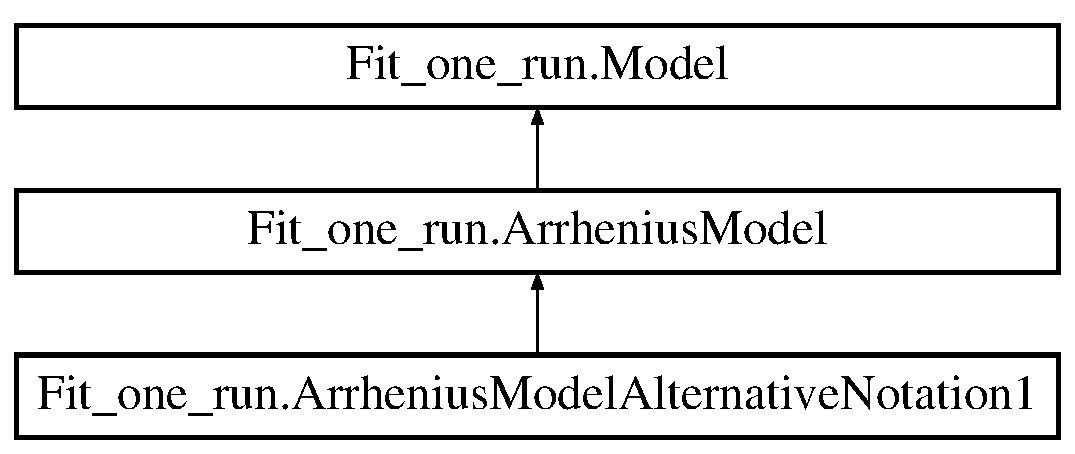
\includegraphics[height=3.000000cm]{classFit__one__run_1_1ArrheniusModelAlternativeNotation1}
\end{center}
\end{figure}
\subsection*{\-Public \-Member \-Functions}
\begin{DoxyCompactItemize}
\item 
\hypertarget{classFit__one__run_1_1ArrheniusModelAlternativeNotation1_a3838b3d98fc08fbf46ee4d52e76a2c1e}{def {\bfseries \-\_\-\-\_\-init\-\_\-\-\_\-}}\label{classFit__one__run_1_1ArrheniusModelAlternativeNotation1_a3838b3d98fc08fbf46ee4d52e76a2c1e}

\item 
def \hyperlink{classFit__one__run_1_1ArrheniusModelAlternativeNotation1_ae5173ca0b3b89ddf7d5407a6023d693f}{calc\-Mass}
\item 
def \hyperlink{classFit__one__run_1_1ArrheniusModelAlternativeNotation1_a0bec2d240a20bdd5b5e4a08bf603c705}{\-Convert\-Kin\-Factors}
\item 
def \hyperlink{classFit__one__run_1_1ArrheniusModelAlternativeNotation1_aa93288bf70f57ce16ae065bf8146f899}{\-Convert\-Kin\-Factors\-To\-Own\-Notation}
\item 
def \hyperlink{classFit__one__run_1_1Model_aa304b32155938a713c33f0dc03a135f3}{plt\-Yield}
\item 
def \hyperlink{classFit__one__run_1_1Model_a9c28d95902adf00f5aaa642f0919fc61}{plt\-Rate}
\item 
def \hyperlink{classFit__one__run_1_1Model_a26fc879ca33c9171ebb4a97bc4b0c46b}{min\-Length\-Of\-Vectors}
\item 
def \hyperlink{classFit__one__run_1_1Model_a98159c954f1f1be2a34be3ea53d11493}{plot}
\item 
def \hyperlink{classFit__one__run_1_1Model_ace9df4177c5ae753dbe190e2f8268149}{derive\-C}
\item 
def \hyperlink{classFit__one__run_1_1Model_a07ae4534de2a6ef241d71facdffb227e}{calc\-Rate}
\item 
def \hyperlink{classFit__one__run_1_1Model_a174aec9b05dbe01ec103f7ba75d6516c}{set\-Param\-Vector}
\item 
def \hyperlink{classFit__one__run_1_1Model_a3c9239f0ac062fdae0bda395636c0372}{\-Param\-Vector}
\item 
def \hyperlink{classFit__one__run_1_1Model_aa2bc4ba19704350fb2ff441734b51b10}{\-Error\-Yield}
\item 
def \hyperlink{classFit__one__run_1_1Model_aad63c345c343f0c7d1cf20135dc0a0e5}{\-Error\-Rate}
\end{DoxyCompactItemize}
\subsection*{\-Public \-Attributes}
\begin{DoxyCompactItemize}
\item 
\hypertarget{classFit__one__run_1_1ArrheniusModelAlternativeNotation1_a08ddb74ee9d11bede62aa27f066899c7}{{\bfseries \-O\-D\-E\-\_\-hmax}}\label{classFit__one__run_1_1ArrheniusModelAlternativeNotation1_a08ddb74ee9d11bede62aa27f066899c7}

\item 
\hypertarget{classFit__one__run_1_1ArrheniusModelAlternativeNotation1_ac77106340545100248d130934535a03c}{{\bfseries \-T0}}\label{classFit__one__run_1_1ArrheniusModelAlternativeNotation1_ac77106340545100248d130934535a03c}

\end{DoxyCompactItemize}


\subsection{\-Detailed \-Description}
\begin{DoxyVerb}Arrhenius model with a notation having a better optimization behaviour: dm/dt=exp[k0-a*(T0/T(t)-1)]*(ms-m). See the documentation for the reference. The parameters to optimize are k0 and a.\end{DoxyVerb}
 

\subsection{\-Member \-Function \-Documentation}
\hypertarget{classFit__one__run_1_1ArrheniusModelAlternativeNotation1_ae5173ca0b3b89ddf7d5407a6023d693f}{\index{\-Fit\-\_\-one\-\_\-run\-::\-Arrhenius\-Model\-Alternative\-Notation1@{\-Fit\-\_\-one\-\_\-run\-::\-Arrhenius\-Model\-Alternative\-Notation1}!calc\-Mass@{calc\-Mass}}
\index{calc\-Mass@{calc\-Mass}!Fit_one_run::ArrheniusModelAlternativeNotation1@{\-Fit\-\_\-one\-\_\-run\-::\-Arrhenius\-Model\-Alternative\-Notation1}}
\subsubsection[{calc\-Mass}]{\setlength{\rightskip}{0pt plus 5cm}def {\bf \-Fit\-\_\-one\-\_\-run.\-Arrhenius\-Model\-Alternative\-Notation1.\-calc\-Mass} (
\begin{DoxyParamCaption}
\item[{}]{self, }
\item[{}]{fgdvc, }
\item[{}]{time, }
\item[{}]{\-T, }
\item[{}]{\-Name}
\end{DoxyParamCaption}
)}}\label{classFit__one__run_1_1ArrheniusModelAlternativeNotation1_ae5173ca0b3b89ddf7d5407a6023d693f}
\begin{DoxyVerb}Outputs the mass(t) using the model specific equation.\end{DoxyVerb}
 

\-Reimplemented from \hyperlink{classFit__one__run_1_1ArrheniusModel_aef95e08280a5f8628b63ea1300227aa7}{\-Fit\-\_\-one\-\_\-run.\-Arrhenius\-Model}.

\hypertarget{classFit__one__run_1_1Model_a07ae4534de2a6ef241d71facdffb227e}{\index{\-Fit\-\_\-one\-\_\-run\-::\-Arrhenius\-Model\-Alternative\-Notation1@{\-Fit\-\_\-one\-\_\-run\-::\-Arrhenius\-Model\-Alternative\-Notation1}!calc\-Rate@{calc\-Rate}}
\index{calc\-Rate@{calc\-Rate}!Fit_one_run::ArrheniusModelAlternativeNotation1@{\-Fit\-\_\-one\-\_\-run\-::\-Arrhenius\-Model\-Alternative\-Notation1}}
\subsubsection[{calc\-Rate}]{\setlength{\rightskip}{0pt plus 5cm}def {\bf \-Fit\-\_\-one\-\_\-run.\-Model.\-calc\-Rate} (
\begin{DoxyParamCaption}
\item[{}]{self, }
\item[{}]{fgdvc, }
\item[{}]{time, }
\item[{}]{\-T, }
\item[{}]{\-Name}
\end{DoxyParamCaption}
)\hspace{0.3cm}{\ttfamily  \mbox{[}inherited\mbox{]}}}}\label{classFit__one__run_1_1Model_a07ae4534de2a6ef241d71facdffb227e}
\begin{DoxyVerb}Generates the Rates using the yields vector and a CDS.\end{DoxyVerb}
 \hypertarget{classFit__one__run_1_1ArrheniusModelAlternativeNotation1_a0bec2d240a20bdd5b5e4a08bf603c705}{\index{\-Fit\-\_\-one\-\_\-run\-::\-Arrhenius\-Model\-Alternative\-Notation1@{\-Fit\-\_\-one\-\_\-run\-::\-Arrhenius\-Model\-Alternative\-Notation1}!\-Convert\-Kin\-Factors@{\-Convert\-Kin\-Factors}}
\index{\-Convert\-Kin\-Factors@{\-Convert\-Kin\-Factors}!Fit_one_run::ArrheniusModelAlternativeNotation1@{\-Fit\-\_\-one\-\_\-run\-::\-Arrhenius\-Model\-Alternative\-Notation1}}
\subsubsection[{\-Convert\-Kin\-Factors}]{\setlength{\rightskip}{0pt plus 5cm}def {\bf \-Fit\-\_\-one\-\_\-run.\-Arrhenius\-Model\-Alternative\-Notation1.\-Convert\-Kin\-Factors} (
\begin{DoxyParamCaption}
\item[{}]{self, }
\item[{}]{\-Parameter\-Vector}
\end{DoxyParamCaption}
)}}\label{classFit__one__run_1_1ArrheniusModelAlternativeNotation1_a0bec2d240a20bdd5b5e4a08bf603c705}
\begin{DoxyVerb}Converts the own kinetic factors back to the standard Arrhenius kinetic factors.\end{DoxyVerb}
 

\-Reimplemented from \hyperlink{classFit__one__run_1_1ArrheniusModel_a2d145de8ceef61b26b3ab701618ebb9d}{\-Fit\-\_\-one\-\_\-run.\-Arrhenius\-Model}.

\hypertarget{classFit__one__run_1_1ArrheniusModelAlternativeNotation1_aa93288bf70f57ce16ae065bf8146f899}{\index{\-Fit\-\_\-one\-\_\-run\-::\-Arrhenius\-Model\-Alternative\-Notation1@{\-Fit\-\_\-one\-\_\-run\-::\-Arrhenius\-Model\-Alternative\-Notation1}!\-Convert\-Kin\-Factors\-To\-Own\-Notation@{\-Convert\-Kin\-Factors\-To\-Own\-Notation}}
\index{\-Convert\-Kin\-Factors\-To\-Own\-Notation@{\-Convert\-Kin\-Factors\-To\-Own\-Notation}!Fit_one_run::ArrheniusModelAlternativeNotation1@{\-Fit\-\_\-one\-\_\-run\-::\-Arrhenius\-Model\-Alternative\-Notation1}}
\subsubsection[{\-Convert\-Kin\-Factors\-To\-Own\-Notation}]{\setlength{\rightskip}{0pt plus 5cm}def {\bf \-Fit\-\_\-one\-\_\-run.\-Arrhenius\-Model\-Alternative\-Notation1.\-Convert\-Kin\-Factors\-To\-Own\-Notation} (
\begin{DoxyParamCaption}
\item[{}]{self, }
\item[{}]{fgdvc, }
\item[{}]{\-Parameter\-Vector, }
\item[{}]{\-Species}
\end{DoxyParamCaption}
)}}\label{classFit__one__run_1_1ArrheniusModelAlternativeNotation1_aa93288bf70f57ce16ae065bf8146f899}
\begin{DoxyVerb}Converts the standard Arrhenius kinetic factors backk to the factors of the own notation.\end{DoxyVerb}
 \hypertarget{classFit__one__run_1_1Model_ace9df4177c5ae753dbe190e2f8268149}{\index{\-Fit\-\_\-one\-\_\-run\-::\-Arrhenius\-Model\-Alternative\-Notation1@{\-Fit\-\_\-one\-\_\-run\-::\-Arrhenius\-Model\-Alternative\-Notation1}!derive\-C@{derive\-C}}
\index{derive\-C@{derive\-C}!Fit_one_run::ArrheniusModelAlternativeNotation1@{\-Fit\-\_\-one\-\_\-run\-::\-Arrhenius\-Model\-Alternative\-Notation1}}
\subsubsection[{derive\-C}]{\setlength{\rightskip}{0pt plus 5cm}def {\bf \-Fit\-\_\-one\-\_\-run.\-Model.\-derive\-C} (
\begin{DoxyParamCaption}
\item[{}]{self, }
\item[{}]{fgdvc, }
\item[{}]{y\-Vector, }
\item[{}]{max\-Vector\-Lenght = {\ttfamily \-None}}
\end{DoxyParamCaption}
)\hspace{0.3cm}{\ttfamily  \mbox{[}inherited\mbox{]}}}}\label{classFit__one__run_1_1Model_ace9df4177c5ae753dbe190e2f8268149}
\begin{DoxyVerb}Returns a CDS of the inputted yVector.\end{DoxyVerb}
 \hypertarget{classFit__one__run_1_1Model_aad63c345c343f0c7d1cf20135dc0a0e5}{\index{\-Fit\-\_\-one\-\_\-run\-::\-Arrhenius\-Model\-Alternative\-Notation1@{\-Fit\-\_\-one\-\_\-run\-::\-Arrhenius\-Model\-Alternative\-Notation1}!\-Error\-Rate@{\-Error\-Rate}}
\index{\-Error\-Rate@{\-Error\-Rate}!Fit_one_run::ArrheniusModelAlternativeNotation1@{\-Fit\-\_\-one\-\_\-run\-::\-Arrhenius\-Model\-Alternative\-Notation1}}
\subsubsection[{\-Error\-Rate}]{\setlength{\rightskip}{0pt plus 5cm}def {\bf \-Fit\-\_\-one\-\_\-run.\-Model.\-Error\-Rate} (
\begin{DoxyParamCaption}
\item[{}]{self, }
\item[{}]{fgdvc, }
\item[{}]{\-Species}
\end{DoxyParamCaption}
)\hspace{0.3cm}{\ttfamily  \mbox{[}inherited\mbox{]}}}}\label{classFit__one__run_1_1Model_aad63c345c343f0c7d1cf20135dc0a0e5}
\begin{DoxyVerb}Returns the absolute deviation per point between the fitted and the original rate curve.\end{DoxyVerb}
 \hypertarget{classFit__one__run_1_1Model_aa2bc4ba19704350fb2ff441734b51b10}{\index{\-Fit\-\_\-one\-\_\-run\-::\-Arrhenius\-Model\-Alternative\-Notation1@{\-Fit\-\_\-one\-\_\-run\-::\-Arrhenius\-Model\-Alternative\-Notation1}!\-Error\-Yield@{\-Error\-Yield}}
\index{\-Error\-Yield@{\-Error\-Yield}!Fit_one_run::ArrheniusModelAlternativeNotation1@{\-Fit\-\_\-one\-\_\-run\-::\-Arrhenius\-Model\-Alternative\-Notation1}}
\subsubsection[{\-Error\-Yield}]{\setlength{\rightskip}{0pt plus 5cm}def {\bf \-Fit\-\_\-one\-\_\-run.\-Model.\-Error\-Yield} (
\begin{DoxyParamCaption}
\item[{}]{self, }
\item[{}]{fgdvc, }
\item[{}]{\-Species}
\end{DoxyParamCaption}
)\hspace{0.3cm}{\ttfamily  \mbox{[}inherited\mbox{]}}}}\label{classFit__one__run_1_1Model_aa2bc4ba19704350fb2ff441734b51b10}
\begin{DoxyVerb}Returns the absolute deviation per point between the fitted and the original yield curve.\end{DoxyVerb}
 \hypertarget{classFit__one__run_1_1Model_a26fc879ca33c9171ebb4a97bc4b0c46b}{\index{\-Fit\-\_\-one\-\_\-run\-::\-Arrhenius\-Model\-Alternative\-Notation1@{\-Fit\-\_\-one\-\_\-run\-::\-Arrhenius\-Model\-Alternative\-Notation1}!min\-Length\-Of\-Vectors@{min\-Length\-Of\-Vectors}}
\index{min\-Length\-Of\-Vectors@{min\-Length\-Of\-Vectors}!Fit_one_run::ArrheniusModelAlternativeNotation1@{\-Fit\-\_\-one\-\_\-run\-::\-Arrhenius\-Model\-Alternative\-Notation1}}
\subsubsection[{min\-Length\-Of\-Vectors}]{\setlength{\rightskip}{0pt plus 5cm}def {\bf \-Fit\-\_\-one\-\_\-run.\-Model.\-min\-Length\-Of\-Vectors} (
\begin{DoxyParamCaption}
\item[{}]{self, }
\item[{}]{fgdvc\-\_\-list}
\end{DoxyParamCaption}
)\hspace{0.3cm}{\ttfamily  \mbox{[}inherited\mbox{]}}}}\label{classFit__one__run_1_1Model_a26fc879ca33c9171ebb4a97bc4b0c46b}
\begin{DoxyVerb}Returns the minimum lenght of a all vectors from the several runs.\end{DoxyVerb}
 \hypertarget{classFit__one__run_1_1Model_a3c9239f0ac062fdae0bda395636c0372}{\index{\-Fit\-\_\-one\-\_\-run\-::\-Arrhenius\-Model\-Alternative\-Notation1@{\-Fit\-\_\-one\-\_\-run\-::\-Arrhenius\-Model\-Alternative\-Notation1}!\-Param\-Vector@{\-Param\-Vector}}
\index{\-Param\-Vector@{\-Param\-Vector}!Fit_one_run::ArrheniusModelAlternativeNotation1@{\-Fit\-\_\-one\-\_\-run\-::\-Arrhenius\-Model\-Alternative\-Notation1}}
\subsubsection[{\-Param\-Vector}]{\setlength{\rightskip}{0pt plus 5cm}def {\bf \-Fit\-\_\-one\-\_\-run.\-Model.\-Param\-Vector} (
\begin{DoxyParamCaption}
\item[{}]{self}
\end{DoxyParamCaption}
)\hspace{0.3cm}{\ttfamily  \mbox{[}inherited\mbox{]}}}}\label{classFit__one__run_1_1Model_a3c9239f0ac062fdae0bda395636c0372}
\begin{DoxyVerb}Returns the Vector containing the kinetic parameter of the Model (refering to the child model).\end{DoxyVerb}
 \hypertarget{classFit__one__run_1_1Model_a98159c954f1f1be2a34be3ea53d11493}{\index{\-Fit\-\_\-one\-\_\-run\-::\-Arrhenius\-Model\-Alternative\-Notation1@{\-Fit\-\_\-one\-\_\-run\-::\-Arrhenius\-Model\-Alternative\-Notation1}!plot@{plot}}
\index{plot@{plot}!Fit_one_run::ArrheniusModelAlternativeNotation1@{\-Fit\-\_\-one\-\_\-run\-::\-Arrhenius\-Model\-Alternative\-Notation1}}
\subsubsection[{plot}]{\setlength{\rightskip}{0pt plus 5cm}def {\bf \-Fit\-\_\-one\-\_\-run.\-Model.\-plot} (
\begin{DoxyParamCaption}
\item[{}]{self, }
\item[{}]{fgdvc\-\_\-list, }
\item[{}]{\-Species}
\end{DoxyParamCaption}
)\hspace{0.3cm}{\ttfamily  \mbox{[}inherited\mbox{]}}}}\label{classFit__one__run_1_1Model_a98159c954f1f1be2a34be3ea53d11493}
\begin{DoxyVerb}Plot the yield and the rates over time with two curves: one is the original data, the other the fitting curve. Also file 'PyrolysisProgramName-Species.out' (e.g. 'CPD-CO2.out') containing the time (s), yields (kg/kg), rates (kg/(kg s)).\end{DoxyVerb}
 \hypertarget{classFit__one__run_1_1Model_a9c28d95902adf00f5aaa642f0919fc61}{\index{\-Fit\-\_\-one\-\_\-run\-::\-Arrhenius\-Model\-Alternative\-Notation1@{\-Fit\-\_\-one\-\_\-run\-::\-Arrhenius\-Model\-Alternative\-Notation1}!plt\-Rate@{plt\-Rate}}
\index{plt\-Rate@{plt\-Rate}!Fit_one_run::ArrheniusModelAlternativeNotation1@{\-Fit\-\_\-one\-\_\-run\-::\-Arrhenius\-Model\-Alternative\-Notation1}}
\subsubsection[{plt\-Rate}]{\setlength{\rightskip}{0pt plus 5cm}def {\bf \-Fit\-\_\-one\-\_\-run.\-Model.\-plt\-Rate} (
\begin{DoxyParamCaption}
\item[{}]{self, }
\item[{}]{fgdvc\-\_\-list, }
\item[{}]{x\-Value\-To\-Plot, }
\item[{}]{y\-Value\-To\-Plot}
\end{DoxyParamCaption}
)\hspace{0.3cm}{\ttfamily  \mbox{[}inherited\mbox{]}}}}\label{classFit__one__run_1_1Model_a9c28d95902adf00f5aaa642f0919fc61}
\begin{DoxyVerb}Plots the rates (to select with yValueToPlot) over Time or Temperature (to slect with xValueToPlot).\end{DoxyVerb}
 \hypertarget{classFit__one__run_1_1Model_aa304b32155938a713c33f0dc03a135f3}{\index{\-Fit\-\_\-one\-\_\-run\-::\-Arrhenius\-Model\-Alternative\-Notation1@{\-Fit\-\_\-one\-\_\-run\-::\-Arrhenius\-Model\-Alternative\-Notation1}!plt\-Yield@{plt\-Yield}}
\index{plt\-Yield@{plt\-Yield}!Fit_one_run::ArrheniusModelAlternativeNotation1@{\-Fit\-\_\-one\-\_\-run\-::\-Arrhenius\-Model\-Alternative\-Notation1}}
\subsubsection[{plt\-Yield}]{\setlength{\rightskip}{0pt plus 5cm}def {\bf \-Fit\-\_\-one\-\_\-run.\-Model.\-plt\-Yield} (
\begin{DoxyParamCaption}
\item[{}]{self, }
\item[{}]{fgdvc\-\_\-list, }
\item[{}]{x\-Value\-To\-Plot, }
\item[{}]{y\-Value\-To\-Plot}
\end{DoxyParamCaption}
)\hspace{0.3cm}{\ttfamily  \mbox{[}inherited\mbox{]}}}}\label{classFit__one__run_1_1Model_aa304b32155938a713c33f0dc03a135f3}
\begin{DoxyVerb}Plots the yields (to select with yValueToPlot) over Time or Temperature (to slect with xValueToPlot).\end{DoxyVerb}
 \hypertarget{classFit__one__run_1_1Model_a174aec9b05dbe01ec103f7ba75d6516c}{\index{\-Fit\-\_\-one\-\_\-run\-::\-Arrhenius\-Model\-Alternative\-Notation1@{\-Fit\-\_\-one\-\_\-run\-::\-Arrhenius\-Model\-Alternative\-Notation1}!set\-Param\-Vector@{set\-Param\-Vector}}
\index{set\-Param\-Vector@{set\-Param\-Vector}!Fit_one_run::ArrheniusModelAlternativeNotation1@{\-Fit\-\_\-one\-\_\-run\-::\-Arrhenius\-Model\-Alternative\-Notation1}}
\subsubsection[{set\-Param\-Vector}]{\setlength{\rightskip}{0pt plus 5cm}def {\bf \-Fit\-\_\-one\-\_\-run.\-Model.\-set\-Param\-Vector} (
\begin{DoxyParamCaption}
\item[{}]{self, }
\item[{}]{\-Parameter\-List}
\end{DoxyParamCaption}
)\hspace{0.3cm}{\ttfamily  \mbox{[}inherited\mbox{]}}}}\label{classFit__one__run_1_1Model_a174aec9b05dbe01ec103f7ba75d6516c}
\begin{DoxyVerb}Sets the Vector containing the kinetic parameter of the Model (refering to the child model).\end{DoxyVerb}
 

\-The documentation for this class was generated from the following file\-:\begin{DoxyCompactItemize}
\item 
/home/map/git/pkp/src/\-Fit\-\_\-one\-\_\-run.\-py\end{DoxyCompactItemize}

\hypertarget{classModels_1_1ArrheniusModelAlternativeNotation2}{\section{\-Models.\-Arrhenius\-Model\-Alternative\-Notation2 \-Class \-Reference}
\label{classModels_1_1ArrheniusModelAlternativeNotation2}\index{\-Models.\-Arrhenius\-Model\-Alternative\-Notation2@{\-Models.\-Arrhenius\-Model\-Alternative\-Notation2}}
}
\-Inheritance diagram for \-Models.\-Arrhenius\-Model\-Alternative\-Notation2\-:\begin{figure}[H]
\begin{center}
\leavevmode
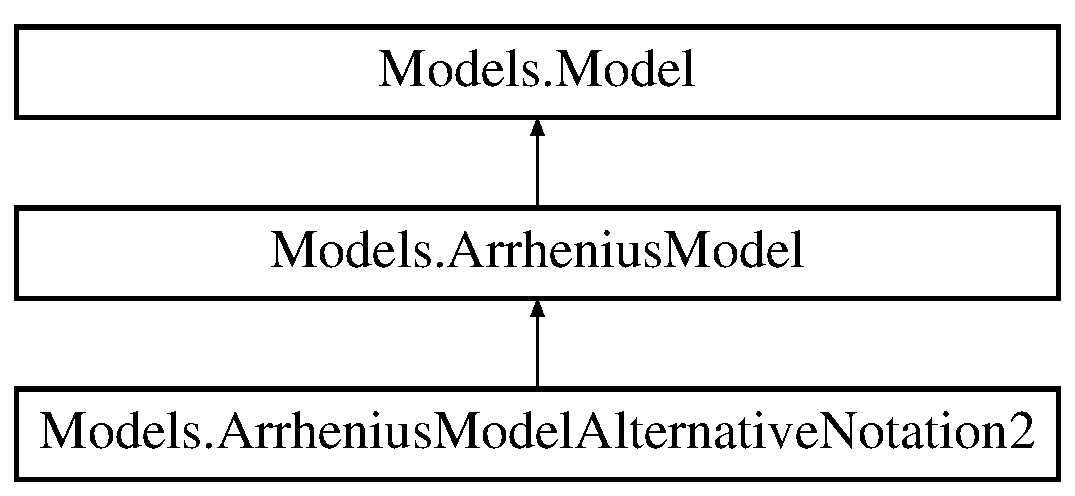
\includegraphics[height=3.000000cm]{classModels_1_1ArrheniusModelAlternativeNotation2}
\end{center}
\end{figure}
\subsection*{\-Public \-Member \-Functions}
\begin{DoxyCompactItemize}
\item 
\hypertarget{classModels_1_1ArrheniusModelAlternativeNotation2_a31e5d19d4c8a3a40e443bda85b5a9ca3}{def {\bfseries \-\_\-\-\_\-init\-\_\-\-\_\-}}\label{classModels_1_1ArrheniusModelAlternativeNotation2_a31e5d19d4c8a3a40e443bda85b5a9ca3}

\item 
def \hyperlink{classModels_1_1ArrheniusModelAlternativeNotation2_aec47f44b01fdbf818fe5839a8c7c17f4}{set\-Min\-Max\-Temp}
\item 
def \hyperlink{classModels_1_1ArrheniusModelAlternativeNotation2_afe70c590fc443e5d91a51485089c513f}{calc\-Mass}
\item 
def \hyperlink{classModels_1_1ArrheniusModelAlternativeNotation2_a82aa3ccadb987ed778dde97edaf5b687}{\-Convert\-Kin\-Factors}
\item 
def \hyperlink{classModels_1_1ArrheniusModelAlternativeNotation2_aca4ecfb8e8796868adc871488d5932c4}{\-Convert\-Kin\-Factors\-To\-Own\-Notation}
\item 
def \hyperlink{classModels_1_1Model_a317ed848b969dbe3a96dd05e8b771900}{plt\-Yield}
\item 
def \hyperlink{classModels_1_1Model_aa35c741babf8f141df48c4021e0664e4}{plt\-Rate}
\item 
def \hyperlink{classModels_1_1Model_a3396d6ca1a7b7d66e55ada8c3c7a509e}{max\-Length\-Of\-Vectors}
\item 
def \hyperlink{classModels_1_1Model_ae404a691e48bfe4eafcdfdd09f1dae48}{plot}
\item 
def \hyperlink{classModels_1_1Model_a010945ed2adff59a7a5fce36025e7a97}{derive\-C}
\item 
def \hyperlink{classModels_1_1Model_a7c9280e33f9e0d46703cebc131008c65}{calc\-Rate}
\item 
def \hyperlink{classModels_1_1Model_a818f207e2a4bd0e9a3720ca611960e5a}{set\-Param\-Vector}
\item 
def \hyperlink{classModels_1_1Model_a13c76a0fe24d43cdc4d21fbc73fa96fa}{\-Param\-Vector}
\item 
def \hyperlink{classModels_1_1Model_ad3e627980d9e781bf7b2c9ff900ca06b}{\-Error\-Yield}
\item 
def \hyperlink{classModels_1_1Model_a3050eb39341f318d8d88b172f88bd240}{\-Error\-Rate}
\item 
def \hyperlink{classModels_1_1Model_adcb987bccae63a742490ea1e6d5f7a74}{mk\-Simple\-Result\-Files}
\item 
def \hyperlink{classModels_1_1Model_ac28252ae5cd6b5ecd4c5d006a0e6567d}{set\-Dt4\-Intergrate}
\end{DoxyCompactItemize}
\subsection*{\-Public \-Attributes}
\begin{DoxyCompactItemize}
\item 
\hypertarget{classModels_1_1ArrheniusModelAlternativeNotation2_af34ea99cbe467aea419df689f3ad2d1a}{{\bfseries \-T\-\_\-min}}\label{classModels_1_1ArrheniusModelAlternativeNotation2_af34ea99cbe467aea419df689f3ad2d1a}

\item 
\hypertarget{classModels_1_1ArrheniusModelAlternativeNotation2_a43499e47431b8f8a00ac3d911d59d889}{{\bfseries \-T\-\_\-max}}\label{classModels_1_1ArrheniusModelAlternativeNotation2_a43499e47431b8f8a00ac3d911d59d889}

\item 
\hypertarget{classModels_1_1ArrheniusModelAlternativeNotation2_a226c031ab761b1c46b2dc0a6718eb340}{{\bfseries const\-Dt}}\label{classModels_1_1ArrheniusModelAlternativeNotation2_a226c031ab761b1c46b2dc0a6718eb340}

\item 
\hypertarget{classModels_1_1ArrheniusModelAlternativeNotation2_a820391809a51812c06ece08248ce30fe}{{\bfseries c}}\label{classModels_1_1ArrheniusModelAlternativeNotation2_a820391809a51812c06ece08248ce30fe}

\item 
\hypertarget{classModels_1_1ArrheniusModelAlternativeNotation2_ada7f810b2f91a9c1454545a058c0e560}{{\bfseries \-O\-D\-E\-\_\-hmax}}\label{classModels_1_1ArrheniusModelAlternativeNotation2_ada7f810b2f91a9c1454545a058c0e560}

\item 
\hypertarget{classModels_1_1ArrheniusModelAlternativeNotation2_a4d09873028a6c0bc11fe0a05016604cc}{{\bfseries fgdvc}}\label{classModels_1_1ArrheniusModelAlternativeNotation2_a4d09873028a6c0bc11fe0a05016604cc}

\item 
\hypertarget{classModels_1_1Model_a3f71983de5f8b86bec47929213b900ec}{{\bfseries const\-Dt\-Vec}}\label{classModels_1_1Model_a3f71983de5f8b86bec47929213b900ec}

\end{DoxyCompactItemize}


\subsection{\-Detailed \-Description}
\begin{DoxyVerb}Arrhenius model with a notation having a better optimization behaviour: dm/dt=exp[c*(b1*(1/T(t)-1/T_min)-b2*(1/T(t)-1/T_max))]*(ms-m); with c=(1/T_max-1/Tmin)**(-1). See the documentation for the reference. The parameters to optimize are b1 and b2.\end{DoxyVerb}
 

\subsection{\-Member \-Function \-Documentation}
\hypertarget{classModels_1_1ArrheniusModelAlternativeNotation2_afe70c590fc443e5d91a51485089c513f}{\index{\-Models\-::\-Arrhenius\-Model\-Alternative\-Notation2@{\-Models\-::\-Arrhenius\-Model\-Alternative\-Notation2}!calc\-Mass@{calc\-Mass}}
\index{calc\-Mass@{calc\-Mass}!Models::ArrheniusModelAlternativeNotation2@{\-Models\-::\-Arrhenius\-Model\-Alternative\-Notation2}}
\subsubsection[{calc\-Mass}]{\setlength{\rightskip}{0pt plus 5cm}def {\bf \-Models.\-Arrhenius\-Model\-Alternative\-Notation2.\-calc\-Mass} (
\begin{DoxyParamCaption}
\item[{}]{self, }
\item[{}]{fgdvc, }
\item[{}]{time, }
\item[{}]{\-T, }
\item[{}]{\-Name}
\end{DoxyParamCaption}
)}}\label{classModels_1_1ArrheniusModelAlternativeNotation2_afe70c590fc443e5d91a51485089c513f}
\begin{DoxyVerb}Outputs the mass(t) using the model specific equation.\end{DoxyVerb}
 

\-Reimplemented from \hyperlink{classModels_1_1ArrheniusModel_abb4fedac573a2f263fd5bb4cd284ce65}{\-Models.\-Arrhenius\-Model}.

\hypertarget{classModels_1_1Model_a7c9280e33f9e0d46703cebc131008c65}{\index{\-Models\-::\-Arrhenius\-Model\-Alternative\-Notation2@{\-Models\-::\-Arrhenius\-Model\-Alternative\-Notation2}!calc\-Rate@{calc\-Rate}}
\index{calc\-Rate@{calc\-Rate}!Models::ArrheniusModelAlternativeNotation2@{\-Models\-::\-Arrhenius\-Model\-Alternative\-Notation2}}
\subsubsection[{calc\-Rate}]{\setlength{\rightskip}{0pt plus 5cm}def {\bf \-Models.\-Model.\-calc\-Rate} (
\begin{DoxyParamCaption}
\item[{}]{self, }
\item[{}]{fgdvc, }
\item[{}]{time, }
\item[{}]{\-T, }
\item[{}]{\-Name}
\end{DoxyParamCaption}
)\hspace{0.3cm}{\ttfamily  \mbox{[}inherited\mbox{]}}}}\label{classModels_1_1Model_a7c9280e33f9e0d46703cebc131008c65}
\begin{DoxyVerb}Generates the Rates using the yields vector and a CDS.\end{DoxyVerb}
 \hypertarget{classModels_1_1ArrheniusModelAlternativeNotation2_a82aa3ccadb987ed778dde97edaf5b687}{\index{\-Models\-::\-Arrhenius\-Model\-Alternative\-Notation2@{\-Models\-::\-Arrhenius\-Model\-Alternative\-Notation2}!\-Convert\-Kin\-Factors@{\-Convert\-Kin\-Factors}}
\index{\-Convert\-Kin\-Factors@{\-Convert\-Kin\-Factors}!Models::ArrheniusModelAlternativeNotation2@{\-Models\-::\-Arrhenius\-Model\-Alternative\-Notation2}}
\subsubsection[{\-Convert\-Kin\-Factors}]{\setlength{\rightskip}{0pt plus 5cm}def {\bf \-Models.\-Arrhenius\-Model\-Alternative\-Notation2.\-Convert\-Kin\-Factors} (
\begin{DoxyParamCaption}
\item[{}]{self, }
\item[{}]{\-Parameter\-Vector}
\end{DoxyParamCaption}
)}}\label{classModels_1_1ArrheniusModelAlternativeNotation2_a82aa3ccadb987ed778dde97edaf5b687}
\begin{DoxyVerb}Converts the own kinetic factors back to the standard Arrhenius kinetic factors.\end{DoxyVerb}
 

\-Reimplemented from \hyperlink{classModels_1_1ArrheniusModel_a946e6177077d67613160aaaedde95faa}{\-Models.\-Arrhenius\-Model}.

\hypertarget{classModels_1_1ArrheniusModelAlternativeNotation2_aca4ecfb8e8796868adc871488d5932c4}{\index{\-Models\-::\-Arrhenius\-Model\-Alternative\-Notation2@{\-Models\-::\-Arrhenius\-Model\-Alternative\-Notation2}!\-Convert\-Kin\-Factors\-To\-Own\-Notation@{\-Convert\-Kin\-Factors\-To\-Own\-Notation}}
\index{\-Convert\-Kin\-Factors\-To\-Own\-Notation@{\-Convert\-Kin\-Factors\-To\-Own\-Notation}!Models::ArrheniusModelAlternativeNotation2@{\-Models\-::\-Arrhenius\-Model\-Alternative\-Notation2}}
\subsubsection[{\-Convert\-Kin\-Factors\-To\-Own\-Notation}]{\setlength{\rightskip}{0pt plus 5cm}def {\bf \-Models.\-Arrhenius\-Model\-Alternative\-Notation2.\-Convert\-Kin\-Factors\-To\-Own\-Notation} (
\begin{DoxyParamCaption}
\item[{}]{self, }
\item[{}]{\-Parameter\-Vector}
\end{DoxyParamCaption}
)}}\label{classModels_1_1ArrheniusModelAlternativeNotation2_aca4ecfb8e8796868adc871488d5932c4}
\begin{DoxyVerb}Converts the standard Arrhenius kinetic factors back to the factors of the own notation.\end{DoxyVerb}
 \hypertarget{classModels_1_1Model_a010945ed2adff59a7a5fce36025e7a97}{\index{\-Models\-::\-Arrhenius\-Model\-Alternative\-Notation2@{\-Models\-::\-Arrhenius\-Model\-Alternative\-Notation2}!derive\-C@{derive\-C}}
\index{derive\-C@{derive\-C}!Models::ArrheniusModelAlternativeNotation2@{\-Models\-::\-Arrhenius\-Model\-Alternative\-Notation2}}
\subsubsection[{derive\-C}]{\setlength{\rightskip}{0pt plus 5cm}def {\bf \-Models.\-Model.\-derive\-C} (
\begin{DoxyParamCaption}
\item[{}]{self, }
\item[{}]{fgdvc, }
\item[{}]{y\-Vector}
\end{DoxyParamCaption}
)\hspace{0.3cm}{\ttfamily  \mbox{[}inherited\mbox{]}}}}\label{classModels_1_1Model_a010945ed2adff59a7a5fce36025e7a97}
\begin{DoxyVerb}Returns a CDS of the inputted yVector.\end{DoxyVerb}
 \hypertarget{classModels_1_1Model_a3050eb39341f318d8d88b172f88bd240}{\index{\-Models\-::\-Arrhenius\-Model\-Alternative\-Notation2@{\-Models\-::\-Arrhenius\-Model\-Alternative\-Notation2}!\-Error\-Rate@{\-Error\-Rate}}
\index{\-Error\-Rate@{\-Error\-Rate}!Models::ArrheniusModelAlternativeNotation2@{\-Models\-::\-Arrhenius\-Model\-Alternative\-Notation2}}
\subsubsection[{\-Error\-Rate}]{\setlength{\rightskip}{0pt plus 5cm}def {\bf \-Models.\-Model.\-Error\-Rate} (
\begin{DoxyParamCaption}
\item[{}]{self, }
\item[{}]{fgdvc, }
\item[{}]{\-Species}
\end{DoxyParamCaption}
)\hspace{0.3cm}{\ttfamily  \mbox{[}inherited\mbox{]}}}}\label{classModels_1_1Model_a3050eb39341f318d8d88b172f88bd240}
\begin{DoxyVerb}Returns the absolute deviation per point between the fitted and the original rate curve.\end{DoxyVerb}
 \hypertarget{classModels_1_1Model_ad3e627980d9e781bf7b2c9ff900ca06b}{\index{\-Models\-::\-Arrhenius\-Model\-Alternative\-Notation2@{\-Models\-::\-Arrhenius\-Model\-Alternative\-Notation2}!\-Error\-Yield@{\-Error\-Yield}}
\index{\-Error\-Yield@{\-Error\-Yield}!Models::ArrheniusModelAlternativeNotation2@{\-Models\-::\-Arrhenius\-Model\-Alternative\-Notation2}}
\subsubsection[{\-Error\-Yield}]{\setlength{\rightskip}{0pt plus 5cm}def {\bf \-Models.\-Model.\-Error\-Yield} (
\begin{DoxyParamCaption}
\item[{}]{self, }
\item[{}]{fgdvc, }
\item[{}]{\-Species}
\end{DoxyParamCaption}
)\hspace{0.3cm}{\ttfamily  \mbox{[}inherited\mbox{]}}}}\label{classModels_1_1Model_ad3e627980d9e781bf7b2c9ff900ca06b}
\begin{DoxyVerb}Returns the absolute deviation per point between the fitted and the original yield curve.\end{DoxyVerb}
 \hypertarget{classModels_1_1Model_a3396d6ca1a7b7d66e55ada8c3c7a509e}{\index{\-Models\-::\-Arrhenius\-Model\-Alternative\-Notation2@{\-Models\-::\-Arrhenius\-Model\-Alternative\-Notation2}!max\-Length\-Of\-Vectors@{max\-Length\-Of\-Vectors}}
\index{max\-Length\-Of\-Vectors@{max\-Length\-Of\-Vectors}!Models::ArrheniusModelAlternativeNotation2@{\-Models\-::\-Arrhenius\-Model\-Alternative\-Notation2}}
\subsubsection[{max\-Length\-Of\-Vectors}]{\setlength{\rightskip}{0pt plus 5cm}def {\bf \-Models.\-Model.\-max\-Length\-Of\-Vectors} (
\begin{DoxyParamCaption}
\item[{}]{self, }
\item[{}]{fgdvc\-\_\-list}
\end{DoxyParamCaption}
)\hspace{0.3cm}{\ttfamily  \mbox{[}inherited\mbox{]}}}}\label{classModels_1_1Model_a3396d6ca1a7b7d66e55ada8c3c7a509e}
\begin{DoxyVerb}Returns the minimum lenght of a all vectors from the several runs.\end{DoxyVerb}
 \hypertarget{classModels_1_1Model_adcb987bccae63a742490ea1e6d5f7a74}{\index{\-Models\-::\-Arrhenius\-Model\-Alternative\-Notation2@{\-Models\-::\-Arrhenius\-Model\-Alternative\-Notation2}!mk\-Simple\-Result\-Files@{mk\-Simple\-Result\-Files}}
\index{mk\-Simple\-Result\-Files@{mk\-Simple\-Result\-Files}!Models::ArrheniusModelAlternativeNotation2@{\-Models\-::\-Arrhenius\-Model\-Alternative\-Notation2}}
\subsubsection[{mk\-Simple\-Result\-Files}]{\setlength{\rightskip}{0pt plus 5cm}def {\bf \-Models.\-Model.\-mk\-Simple\-Result\-Files} (
\begin{DoxyParamCaption}
\item[{}]{self, }
\item[{}]{fgdvc\-\_\-list, }
\item[{}]{\-Species}
\end{DoxyParamCaption}
)\hspace{0.3cm}{\ttfamily  \mbox{[}inherited\mbox{]}}}}\label{classModels_1_1Model_adcb987bccae63a742490ea1e6d5f7a74}
\begin{DoxyVerb}Simple result file if no fitting is carried out. Writes only the transformed results into a file.\end{DoxyVerb}
 \hypertarget{classModels_1_1Model_a13c76a0fe24d43cdc4d21fbc73fa96fa}{\index{\-Models\-::\-Arrhenius\-Model\-Alternative\-Notation2@{\-Models\-::\-Arrhenius\-Model\-Alternative\-Notation2}!\-Param\-Vector@{\-Param\-Vector}}
\index{\-Param\-Vector@{\-Param\-Vector}!Models::ArrheniusModelAlternativeNotation2@{\-Models\-::\-Arrhenius\-Model\-Alternative\-Notation2}}
\subsubsection[{\-Param\-Vector}]{\setlength{\rightskip}{0pt plus 5cm}def {\bf \-Models.\-Model.\-Param\-Vector} (
\begin{DoxyParamCaption}
\item[{}]{self}
\end{DoxyParamCaption}
)\hspace{0.3cm}{\ttfamily  \mbox{[}inherited\mbox{]}}}}\label{classModels_1_1Model_a13c76a0fe24d43cdc4d21fbc73fa96fa}
\begin{DoxyVerb}Returns the Vector containing the kinetic parameter of the Model (refering to the child model).\end{DoxyVerb}
 \hypertarget{classModels_1_1Model_ae404a691e48bfe4eafcdfdd09f1dae48}{\index{\-Models\-::\-Arrhenius\-Model\-Alternative\-Notation2@{\-Models\-::\-Arrhenius\-Model\-Alternative\-Notation2}!plot@{plot}}
\index{plot@{plot}!Models::ArrheniusModelAlternativeNotation2@{\-Models\-::\-Arrhenius\-Model\-Alternative\-Notation2}}
\subsubsection[{plot}]{\setlength{\rightskip}{0pt plus 5cm}def {\bf \-Models.\-Model.\-plot} (
\begin{DoxyParamCaption}
\item[{}]{self, }
\item[{}]{fgdvc\-\_\-list, }
\item[{}]{\-Species}
\end{DoxyParamCaption}
)\hspace{0.3cm}{\ttfamily  \mbox{[}inherited\mbox{]}}}}\label{classModels_1_1Model_ae404a691e48bfe4eafcdfdd09f1dae48}
\begin{DoxyVerb}Plot the yield and the rates over time with two curves: one is the original data, the other the fitting curve. Also file 'PyrolysisProgramName-Species.out' (e.g. 'CPD-CO2.out') containing the time (s), yields (kg/kg), rates (kg/(kg s)).\end{DoxyVerb}
 \hypertarget{classModels_1_1Model_aa35c741babf8f141df48c4021e0664e4}{\index{\-Models\-::\-Arrhenius\-Model\-Alternative\-Notation2@{\-Models\-::\-Arrhenius\-Model\-Alternative\-Notation2}!plt\-Rate@{plt\-Rate}}
\index{plt\-Rate@{plt\-Rate}!Models::ArrheniusModelAlternativeNotation2@{\-Models\-::\-Arrhenius\-Model\-Alternative\-Notation2}}
\subsubsection[{plt\-Rate}]{\setlength{\rightskip}{0pt plus 5cm}def {\bf \-Models.\-Model.\-plt\-Rate} (
\begin{DoxyParamCaption}
\item[{}]{self, }
\item[{}]{fgdvc\-\_\-list, }
\item[{}]{x\-Value\-To\-Plot, }
\item[{}]{y\-Value\-To\-Plot}
\end{DoxyParamCaption}
)\hspace{0.3cm}{\ttfamily  \mbox{[}inherited\mbox{]}}}}\label{classModels_1_1Model_aa35c741babf8f141df48c4021e0664e4}
\begin{DoxyVerb}Plots the rates (to select with yValueToPlot) over Time or Temperature (to slect with xValueToPlot).\end{DoxyVerb}
 \hypertarget{classModels_1_1Model_a317ed848b969dbe3a96dd05e8b771900}{\index{\-Models\-::\-Arrhenius\-Model\-Alternative\-Notation2@{\-Models\-::\-Arrhenius\-Model\-Alternative\-Notation2}!plt\-Yield@{plt\-Yield}}
\index{plt\-Yield@{plt\-Yield}!Models::ArrheniusModelAlternativeNotation2@{\-Models\-::\-Arrhenius\-Model\-Alternative\-Notation2}}
\subsubsection[{plt\-Yield}]{\setlength{\rightskip}{0pt plus 5cm}def {\bf \-Models.\-Model.\-plt\-Yield} (
\begin{DoxyParamCaption}
\item[{}]{self, }
\item[{}]{fgdvc\-\_\-list, }
\item[{}]{x\-Value\-To\-Plot, }
\item[{}]{y\-Value\-To\-Plot}
\end{DoxyParamCaption}
)\hspace{0.3cm}{\ttfamily  \mbox{[}inherited\mbox{]}}}}\label{classModels_1_1Model_a317ed848b969dbe3a96dd05e8b771900}
\begin{DoxyVerb}Plots the yields (to select with yValueToPlot) over Time or Temperature (to slect with xValueToPlot).\end{DoxyVerb}
 \hypertarget{classModels_1_1Model_ac28252ae5cd6b5ecd4c5d006a0e6567d}{\index{\-Models\-::\-Arrhenius\-Model\-Alternative\-Notation2@{\-Models\-::\-Arrhenius\-Model\-Alternative\-Notation2}!set\-Dt4\-Intergrate@{set\-Dt4\-Intergrate}}
\index{set\-Dt4\-Intergrate@{set\-Dt4\-Intergrate}!Models::ArrheniusModelAlternativeNotation2@{\-Models\-::\-Arrhenius\-Model\-Alternative\-Notation2}}
\subsubsection[{set\-Dt4\-Intergrate}]{\setlength{\rightskip}{0pt plus 5cm}def {\bf \-Models.\-Model.\-set\-Dt4\-Intergrate} (
\begin{DoxyParamCaption}
\item[{}]{self, }
\item[{}]{constant\-Dt}
\end{DoxyParamCaption}
)\hspace{0.3cm}{\ttfamily  \mbox{[}inherited\mbox{]}}}}\label{classModels_1_1Model_ac28252ae5cd6b5ecd4c5d006a0e6567d}
\begin{DoxyVerb}constantDt allows the option to define numerical time step to solve the ODE. The outputted results ever equal the imported time list (when applying method calcMass Time = [t0,t1,t2,t3,t4]. If these time steps are too large, then is this defined dt used to solve the ODE and the results are linear interploated that way that they correspond to the imported time vector. To reset it, just set constantDt to False.\end{DoxyVerb}
 \hypertarget{classModels_1_1ArrheniusModelAlternativeNotation2_aec47f44b01fdbf818fe5839a8c7c17f4}{\index{\-Models\-::\-Arrhenius\-Model\-Alternative\-Notation2@{\-Models\-::\-Arrhenius\-Model\-Alternative\-Notation2}!set\-Min\-Max\-Temp@{set\-Min\-Max\-Temp}}
\index{set\-Min\-Max\-Temp@{set\-Min\-Max\-Temp}!Models::ArrheniusModelAlternativeNotation2@{\-Models\-::\-Arrhenius\-Model\-Alternative\-Notation2}}
\subsubsection[{set\-Min\-Max\-Temp}]{\setlength{\rightskip}{0pt plus 5cm}def {\bf \-Models.\-Arrhenius\-Model\-Alternative\-Notation2.\-set\-Min\-Max\-Temp} (
\begin{DoxyParamCaption}
\item[{}]{self, }
\item[{}]{\-Tmin, }
\item[{}]{\-Tmax}
\end{DoxyParamCaption}
)}}\label{classModels_1_1ArrheniusModelAlternativeNotation2_aec47f44b01fdbf818fe5839a8c7c17f4}
\begin{DoxyVerb}Sets the temperature constants, see the equation.\end{DoxyVerb}
 \hypertarget{classModels_1_1Model_a818f207e2a4bd0e9a3720ca611960e5a}{\index{\-Models\-::\-Arrhenius\-Model\-Alternative\-Notation2@{\-Models\-::\-Arrhenius\-Model\-Alternative\-Notation2}!set\-Param\-Vector@{set\-Param\-Vector}}
\index{set\-Param\-Vector@{set\-Param\-Vector}!Models::ArrheniusModelAlternativeNotation2@{\-Models\-::\-Arrhenius\-Model\-Alternative\-Notation2}}
\subsubsection[{set\-Param\-Vector}]{\setlength{\rightskip}{0pt plus 5cm}def {\bf \-Models.\-Model.\-set\-Param\-Vector} (
\begin{DoxyParamCaption}
\item[{}]{self, }
\item[{}]{\-Parameter\-List}
\end{DoxyParamCaption}
)\hspace{0.3cm}{\ttfamily  \mbox{[}inherited\mbox{]}}}}\label{classModels_1_1Model_a818f207e2a4bd0e9a3720ca611960e5a}
\begin{DoxyVerb}Sets the Vector containing the kinetic parameter of the Model (refering to the child model).\end{DoxyVerb}
 

\-The documentation for this class was generated from the following file\-:\begin{DoxyCompactItemize}
\item 
/home/map/git/pkp/src/\-Models.\-py\end{DoxyCompactItemize}

\hypertarget{classFit__one__run_1_1ArrheniusModelAlternativeNotation2}{\section{\-Fit\-\_\-one\-\_\-run.\-Arrhenius\-Model\-Alternative\-Notation2 \-Class \-Reference}
\label{classFit__one__run_1_1ArrheniusModelAlternativeNotation2}\index{\-Fit\-\_\-one\-\_\-run.\-Arrhenius\-Model\-Alternative\-Notation2@{\-Fit\-\_\-one\-\_\-run.\-Arrhenius\-Model\-Alternative\-Notation2}}
}
\-Inheritance diagram for \-Fit\-\_\-one\-\_\-run.\-Arrhenius\-Model\-Alternative\-Notation2\-:\begin{figure}[H]
\begin{center}
\leavevmode
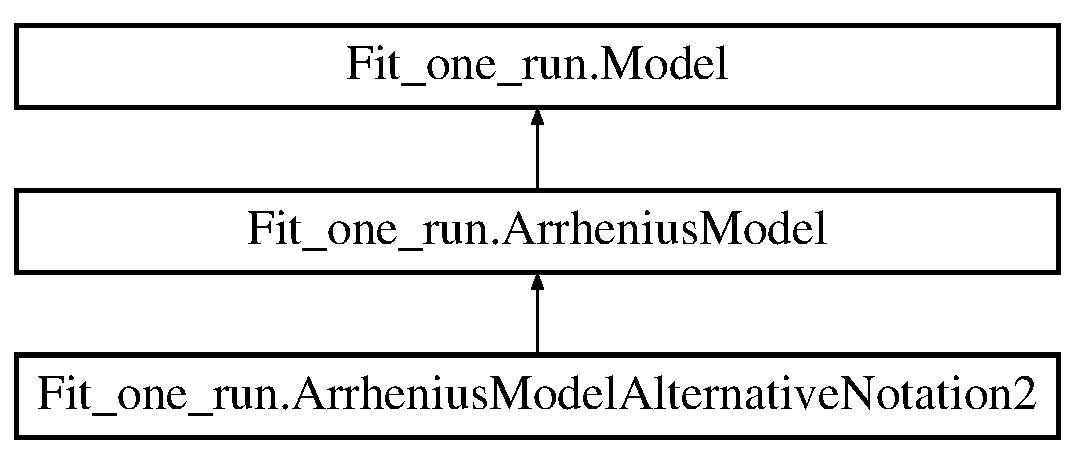
\includegraphics[height=3.000000cm]{classFit__one__run_1_1ArrheniusModelAlternativeNotation2}
\end{center}
\end{figure}
\subsection*{\-Public \-Member \-Functions}
\begin{DoxyCompactItemize}
\item 
\hypertarget{classFit__one__run_1_1ArrheniusModelAlternativeNotation2_ab0e6cc19bc075aceb03286fdf1178b33}{def {\bfseries \-\_\-\-\_\-init\-\_\-\-\_\-}}\label{classFit__one__run_1_1ArrheniusModelAlternativeNotation2_ab0e6cc19bc075aceb03286fdf1178b33}

\item 
def \hyperlink{classFit__one__run_1_1ArrheniusModelAlternativeNotation2_ad2b7981d11c82b7fb90f476396655f3f}{calc\-Mass}
\item 
def \hyperlink{classFit__one__run_1_1ArrheniusModelAlternativeNotation2_a4f6e2eb68a60c1dbdbb6176ad7cf508a}{\-Convert\-Kin\-Factors}
\item 
def \hyperlink{classFit__one__run_1_1ArrheniusModelAlternativeNotation2_ac12a7c92f1991306e31ff67564de4126}{\-Convert\-Kin\-Factors\-To\-Own\-Notation}
\item 
def \hyperlink{classFit__one__run_1_1Model_aa304b32155938a713c33f0dc03a135f3}{plt\-Yield}
\item 
def \hyperlink{classFit__one__run_1_1Model_a9c28d95902adf00f5aaa642f0919fc61}{plt\-Rate}
\item 
def \hyperlink{classFit__one__run_1_1Model_a26fc879ca33c9171ebb4a97bc4b0c46b}{min\-Length\-Of\-Vectors}
\item 
def \hyperlink{classFit__one__run_1_1Model_a98159c954f1f1be2a34be3ea53d11493}{plot}
\item 
def \hyperlink{classFit__one__run_1_1Model_ace9df4177c5ae753dbe190e2f8268149}{derive\-C}
\item 
def \hyperlink{classFit__one__run_1_1Model_a07ae4534de2a6ef241d71facdffb227e}{calc\-Rate}
\item 
def \hyperlink{classFit__one__run_1_1Model_a174aec9b05dbe01ec103f7ba75d6516c}{set\-Param\-Vector}
\item 
def \hyperlink{classFit__one__run_1_1Model_a3c9239f0ac062fdae0bda395636c0372}{\-Param\-Vector}
\item 
def \hyperlink{classFit__one__run_1_1Model_aa2bc4ba19704350fb2ff441734b51b10}{\-Error\-Yield}
\item 
def \hyperlink{classFit__one__run_1_1Model_aad63c345c343f0c7d1cf20135dc0a0e5}{\-Error\-Rate}
\end{DoxyCompactItemize}
\subsection*{\-Public \-Attributes}
\begin{DoxyCompactItemize}
\item 
\hypertarget{classFit__one__run_1_1ArrheniusModelAlternativeNotation2_a5c8d99a0bfb1d0b09ece9a03e0e7d614}{{\bfseries \-T\-\_\-min}}\label{classFit__one__run_1_1ArrheniusModelAlternativeNotation2_a5c8d99a0bfb1d0b09ece9a03e0e7d614}

\item 
\hypertarget{classFit__one__run_1_1ArrheniusModelAlternativeNotation2_ae15bee9047ddc788c76d5f3d37da05b7}{{\bfseries \-T\-\_\-max}}\label{classFit__one__run_1_1ArrheniusModelAlternativeNotation2_ae15bee9047ddc788c76d5f3d37da05b7}

\item 
\hypertarget{classFit__one__run_1_1ArrheniusModelAlternativeNotation2_a1112181ab62d1cb3520fe048bd242324}{{\bfseries c}}\label{classFit__one__run_1_1ArrheniusModelAlternativeNotation2_a1112181ab62d1cb3520fe048bd242324}

\item 
\hypertarget{classFit__one__run_1_1ArrheniusModelAlternativeNotation2_a1b0fc9003a29db87bd8de0e86223b4cb}{{\bfseries \-O\-D\-E\-\_\-hmax}}\label{classFit__one__run_1_1ArrheniusModelAlternativeNotation2_a1b0fc9003a29db87bd8de0e86223b4cb}

\item 
\hypertarget{classFit__one__run_1_1ArrheniusModelAlternativeNotation2_a82c2af40105ee8082c9ce161fa743f9e}{{\bfseries fgdvc}}\label{classFit__one__run_1_1ArrheniusModelAlternativeNotation2_a82c2af40105ee8082c9ce161fa743f9e}

\end{DoxyCompactItemize}


\subsection{\-Detailed \-Description}
\begin{DoxyVerb}Arrhenius model with a notation having a better optimization behaviour: dm/dt=exp[c*(b1*(1/T(t)-1/T_min)-b2*(1/T(t)-1/T_max))]*(ms-m); with c=(1/T_max-1/Tmin)**(-1). See the documentation for the reference. The parameters to optimize are b1 and b2.\end{DoxyVerb}
 

\subsection{\-Member \-Function \-Documentation}
\hypertarget{classFit__one__run_1_1ArrheniusModelAlternativeNotation2_ad2b7981d11c82b7fb90f476396655f3f}{\index{\-Fit\-\_\-one\-\_\-run\-::\-Arrhenius\-Model\-Alternative\-Notation2@{\-Fit\-\_\-one\-\_\-run\-::\-Arrhenius\-Model\-Alternative\-Notation2}!calc\-Mass@{calc\-Mass}}
\index{calc\-Mass@{calc\-Mass}!Fit_one_run::ArrheniusModelAlternativeNotation2@{\-Fit\-\_\-one\-\_\-run\-::\-Arrhenius\-Model\-Alternative\-Notation2}}
\subsubsection[{calc\-Mass}]{\setlength{\rightskip}{0pt plus 5cm}def {\bf \-Fit\-\_\-one\-\_\-run.\-Arrhenius\-Model\-Alternative\-Notation2.\-calc\-Mass} (
\begin{DoxyParamCaption}
\item[{}]{self, }
\item[{}]{fgdvc, }
\item[{}]{time, }
\item[{}]{\-T, }
\item[{}]{\-Name}
\end{DoxyParamCaption}
)}}\label{classFit__one__run_1_1ArrheniusModelAlternativeNotation2_ad2b7981d11c82b7fb90f476396655f3f}
\begin{DoxyVerb}Outputs the mass(t) using the model specific equation.\end{DoxyVerb}
 

\-Reimplemented from \hyperlink{classFit__one__run_1_1ArrheniusModel_aef95e08280a5f8628b63ea1300227aa7}{\-Fit\-\_\-one\-\_\-run.\-Arrhenius\-Model}.

\hypertarget{classFit__one__run_1_1Model_a07ae4534de2a6ef241d71facdffb227e}{\index{\-Fit\-\_\-one\-\_\-run\-::\-Arrhenius\-Model\-Alternative\-Notation2@{\-Fit\-\_\-one\-\_\-run\-::\-Arrhenius\-Model\-Alternative\-Notation2}!calc\-Rate@{calc\-Rate}}
\index{calc\-Rate@{calc\-Rate}!Fit_one_run::ArrheniusModelAlternativeNotation2@{\-Fit\-\_\-one\-\_\-run\-::\-Arrhenius\-Model\-Alternative\-Notation2}}
\subsubsection[{calc\-Rate}]{\setlength{\rightskip}{0pt plus 5cm}def {\bf \-Fit\-\_\-one\-\_\-run.\-Model.\-calc\-Rate} (
\begin{DoxyParamCaption}
\item[{}]{self, }
\item[{}]{fgdvc, }
\item[{}]{time, }
\item[{}]{\-T, }
\item[{}]{\-Name}
\end{DoxyParamCaption}
)\hspace{0.3cm}{\ttfamily  \mbox{[}inherited\mbox{]}}}}\label{classFit__one__run_1_1Model_a07ae4534de2a6ef241d71facdffb227e}
\begin{DoxyVerb}Generates the Rates using the yields vector and a CDS.\end{DoxyVerb}
 \hypertarget{classFit__one__run_1_1ArrheniusModelAlternativeNotation2_a4f6e2eb68a60c1dbdbb6176ad7cf508a}{\index{\-Fit\-\_\-one\-\_\-run\-::\-Arrhenius\-Model\-Alternative\-Notation2@{\-Fit\-\_\-one\-\_\-run\-::\-Arrhenius\-Model\-Alternative\-Notation2}!\-Convert\-Kin\-Factors@{\-Convert\-Kin\-Factors}}
\index{\-Convert\-Kin\-Factors@{\-Convert\-Kin\-Factors}!Fit_one_run::ArrheniusModelAlternativeNotation2@{\-Fit\-\_\-one\-\_\-run\-::\-Arrhenius\-Model\-Alternative\-Notation2}}
\subsubsection[{\-Convert\-Kin\-Factors}]{\setlength{\rightskip}{0pt plus 5cm}def {\bf \-Fit\-\_\-one\-\_\-run.\-Arrhenius\-Model\-Alternative\-Notation2.\-Convert\-Kin\-Factors} (
\begin{DoxyParamCaption}
\item[{}]{self, }
\item[{}]{\-Parameter\-Vector}
\end{DoxyParamCaption}
)}}\label{classFit__one__run_1_1ArrheniusModelAlternativeNotation2_a4f6e2eb68a60c1dbdbb6176ad7cf508a}
\begin{DoxyVerb}Converts the own kinetic factors back to the standard Arrhenius kinetic factors.\end{DoxyVerb}
 

\-Reimplemented from \hyperlink{classFit__one__run_1_1ArrheniusModel_a2d145de8ceef61b26b3ab701618ebb9d}{\-Fit\-\_\-one\-\_\-run.\-Arrhenius\-Model}.

\hypertarget{classFit__one__run_1_1ArrheniusModelAlternativeNotation2_ac12a7c92f1991306e31ff67564de4126}{\index{\-Fit\-\_\-one\-\_\-run\-::\-Arrhenius\-Model\-Alternative\-Notation2@{\-Fit\-\_\-one\-\_\-run\-::\-Arrhenius\-Model\-Alternative\-Notation2}!\-Convert\-Kin\-Factors\-To\-Own\-Notation@{\-Convert\-Kin\-Factors\-To\-Own\-Notation}}
\index{\-Convert\-Kin\-Factors\-To\-Own\-Notation@{\-Convert\-Kin\-Factors\-To\-Own\-Notation}!Fit_one_run::ArrheniusModelAlternativeNotation2@{\-Fit\-\_\-one\-\_\-run\-::\-Arrhenius\-Model\-Alternative\-Notation2}}
\subsubsection[{\-Convert\-Kin\-Factors\-To\-Own\-Notation}]{\setlength{\rightskip}{0pt plus 5cm}def {\bf \-Fit\-\_\-one\-\_\-run.\-Arrhenius\-Model\-Alternative\-Notation2.\-Convert\-Kin\-Factors\-To\-Own\-Notation} (
\begin{DoxyParamCaption}
\item[{}]{self, }
\item[{}]{fgdvc, }
\item[{}]{\-Parameter\-Vector}
\end{DoxyParamCaption}
)}}\label{classFit__one__run_1_1ArrheniusModelAlternativeNotation2_ac12a7c92f1991306e31ff67564de4126}
\begin{DoxyVerb}Converts the standard Arrhenius kinetic factors backk to the factors of the own notation.\end{DoxyVerb}
 \hypertarget{classFit__one__run_1_1Model_ace9df4177c5ae753dbe190e2f8268149}{\index{\-Fit\-\_\-one\-\_\-run\-::\-Arrhenius\-Model\-Alternative\-Notation2@{\-Fit\-\_\-one\-\_\-run\-::\-Arrhenius\-Model\-Alternative\-Notation2}!derive\-C@{derive\-C}}
\index{derive\-C@{derive\-C}!Fit_one_run::ArrheniusModelAlternativeNotation2@{\-Fit\-\_\-one\-\_\-run\-::\-Arrhenius\-Model\-Alternative\-Notation2}}
\subsubsection[{derive\-C}]{\setlength{\rightskip}{0pt plus 5cm}def {\bf \-Fit\-\_\-one\-\_\-run.\-Model.\-derive\-C} (
\begin{DoxyParamCaption}
\item[{}]{self, }
\item[{}]{fgdvc, }
\item[{}]{y\-Vector, }
\item[{}]{max\-Vector\-Lenght = {\ttfamily \-None}}
\end{DoxyParamCaption}
)\hspace{0.3cm}{\ttfamily  \mbox{[}inherited\mbox{]}}}}\label{classFit__one__run_1_1Model_ace9df4177c5ae753dbe190e2f8268149}
\begin{DoxyVerb}Returns a CDS of the inputted yVector.\end{DoxyVerb}
 \hypertarget{classFit__one__run_1_1Model_aad63c345c343f0c7d1cf20135dc0a0e5}{\index{\-Fit\-\_\-one\-\_\-run\-::\-Arrhenius\-Model\-Alternative\-Notation2@{\-Fit\-\_\-one\-\_\-run\-::\-Arrhenius\-Model\-Alternative\-Notation2}!\-Error\-Rate@{\-Error\-Rate}}
\index{\-Error\-Rate@{\-Error\-Rate}!Fit_one_run::ArrheniusModelAlternativeNotation2@{\-Fit\-\_\-one\-\_\-run\-::\-Arrhenius\-Model\-Alternative\-Notation2}}
\subsubsection[{\-Error\-Rate}]{\setlength{\rightskip}{0pt plus 5cm}def {\bf \-Fit\-\_\-one\-\_\-run.\-Model.\-Error\-Rate} (
\begin{DoxyParamCaption}
\item[{}]{self, }
\item[{}]{fgdvc, }
\item[{}]{\-Species}
\end{DoxyParamCaption}
)\hspace{0.3cm}{\ttfamily  \mbox{[}inherited\mbox{]}}}}\label{classFit__one__run_1_1Model_aad63c345c343f0c7d1cf20135dc0a0e5}
\begin{DoxyVerb}Returns the absolute deviation per point between the fitted and the original rate curve.\end{DoxyVerb}
 \hypertarget{classFit__one__run_1_1Model_aa2bc4ba19704350fb2ff441734b51b10}{\index{\-Fit\-\_\-one\-\_\-run\-::\-Arrhenius\-Model\-Alternative\-Notation2@{\-Fit\-\_\-one\-\_\-run\-::\-Arrhenius\-Model\-Alternative\-Notation2}!\-Error\-Yield@{\-Error\-Yield}}
\index{\-Error\-Yield@{\-Error\-Yield}!Fit_one_run::ArrheniusModelAlternativeNotation2@{\-Fit\-\_\-one\-\_\-run\-::\-Arrhenius\-Model\-Alternative\-Notation2}}
\subsubsection[{\-Error\-Yield}]{\setlength{\rightskip}{0pt plus 5cm}def {\bf \-Fit\-\_\-one\-\_\-run.\-Model.\-Error\-Yield} (
\begin{DoxyParamCaption}
\item[{}]{self, }
\item[{}]{fgdvc, }
\item[{}]{\-Species}
\end{DoxyParamCaption}
)\hspace{0.3cm}{\ttfamily  \mbox{[}inherited\mbox{]}}}}\label{classFit__one__run_1_1Model_aa2bc4ba19704350fb2ff441734b51b10}
\begin{DoxyVerb}Returns the absolute deviation per point between the fitted and the original yield curve.\end{DoxyVerb}
 \hypertarget{classFit__one__run_1_1Model_a26fc879ca33c9171ebb4a97bc4b0c46b}{\index{\-Fit\-\_\-one\-\_\-run\-::\-Arrhenius\-Model\-Alternative\-Notation2@{\-Fit\-\_\-one\-\_\-run\-::\-Arrhenius\-Model\-Alternative\-Notation2}!min\-Length\-Of\-Vectors@{min\-Length\-Of\-Vectors}}
\index{min\-Length\-Of\-Vectors@{min\-Length\-Of\-Vectors}!Fit_one_run::ArrheniusModelAlternativeNotation2@{\-Fit\-\_\-one\-\_\-run\-::\-Arrhenius\-Model\-Alternative\-Notation2}}
\subsubsection[{min\-Length\-Of\-Vectors}]{\setlength{\rightskip}{0pt plus 5cm}def {\bf \-Fit\-\_\-one\-\_\-run.\-Model.\-min\-Length\-Of\-Vectors} (
\begin{DoxyParamCaption}
\item[{}]{self, }
\item[{}]{fgdvc\-\_\-list}
\end{DoxyParamCaption}
)\hspace{0.3cm}{\ttfamily  \mbox{[}inherited\mbox{]}}}}\label{classFit__one__run_1_1Model_a26fc879ca33c9171ebb4a97bc4b0c46b}
\begin{DoxyVerb}Returns the minimum lenght of a all vectors from the several runs.\end{DoxyVerb}
 \hypertarget{classFit__one__run_1_1Model_a3c9239f0ac062fdae0bda395636c0372}{\index{\-Fit\-\_\-one\-\_\-run\-::\-Arrhenius\-Model\-Alternative\-Notation2@{\-Fit\-\_\-one\-\_\-run\-::\-Arrhenius\-Model\-Alternative\-Notation2}!\-Param\-Vector@{\-Param\-Vector}}
\index{\-Param\-Vector@{\-Param\-Vector}!Fit_one_run::ArrheniusModelAlternativeNotation2@{\-Fit\-\_\-one\-\_\-run\-::\-Arrhenius\-Model\-Alternative\-Notation2}}
\subsubsection[{\-Param\-Vector}]{\setlength{\rightskip}{0pt plus 5cm}def {\bf \-Fit\-\_\-one\-\_\-run.\-Model.\-Param\-Vector} (
\begin{DoxyParamCaption}
\item[{}]{self}
\end{DoxyParamCaption}
)\hspace{0.3cm}{\ttfamily  \mbox{[}inherited\mbox{]}}}}\label{classFit__one__run_1_1Model_a3c9239f0ac062fdae0bda395636c0372}
\begin{DoxyVerb}Returns the Vector containing the kinetic parameter of the Model (refering to the child model).\end{DoxyVerb}
 \hypertarget{classFit__one__run_1_1Model_a98159c954f1f1be2a34be3ea53d11493}{\index{\-Fit\-\_\-one\-\_\-run\-::\-Arrhenius\-Model\-Alternative\-Notation2@{\-Fit\-\_\-one\-\_\-run\-::\-Arrhenius\-Model\-Alternative\-Notation2}!plot@{plot}}
\index{plot@{plot}!Fit_one_run::ArrheniusModelAlternativeNotation2@{\-Fit\-\_\-one\-\_\-run\-::\-Arrhenius\-Model\-Alternative\-Notation2}}
\subsubsection[{plot}]{\setlength{\rightskip}{0pt plus 5cm}def {\bf \-Fit\-\_\-one\-\_\-run.\-Model.\-plot} (
\begin{DoxyParamCaption}
\item[{}]{self, }
\item[{}]{fgdvc\-\_\-list, }
\item[{}]{\-Species}
\end{DoxyParamCaption}
)\hspace{0.3cm}{\ttfamily  \mbox{[}inherited\mbox{]}}}}\label{classFit__one__run_1_1Model_a98159c954f1f1be2a34be3ea53d11493}
\begin{DoxyVerb}Plot the yield and the rates over time with two curves: one is the original data, the other the fitting curve. Also file 'PyrolysisProgramName-Species.out' (e.g. 'CPD-CO2.out') containing the time (s), yields (kg/kg), rates (kg/(kg s)).\end{DoxyVerb}
 \hypertarget{classFit__one__run_1_1Model_a9c28d95902adf00f5aaa642f0919fc61}{\index{\-Fit\-\_\-one\-\_\-run\-::\-Arrhenius\-Model\-Alternative\-Notation2@{\-Fit\-\_\-one\-\_\-run\-::\-Arrhenius\-Model\-Alternative\-Notation2}!plt\-Rate@{plt\-Rate}}
\index{plt\-Rate@{plt\-Rate}!Fit_one_run::ArrheniusModelAlternativeNotation2@{\-Fit\-\_\-one\-\_\-run\-::\-Arrhenius\-Model\-Alternative\-Notation2}}
\subsubsection[{plt\-Rate}]{\setlength{\rightskip}{0pt plus 5cm}def {\bf \-Fit\-\_\-one\-\_\-run.\-Model.\-plt\-Rate} (
\begin{DoxyParamCaption}
\item[{}]{self, }
\item[{}]{fgdvc\-\_\-list, }
\item[{}]{x\-Value\-To\-Plot, }
\item[{}]{y\-Value\-To\-Plot}
\end{DoxyParamCaption}
)\hspace{0.3cm}{\ttfamily  \mbox{[}inherited\mbox{]}}}}\label{classFit__one__run_1_1Model_a9c28d95902adf00f5aaa642f0919fc61}
\begin{DoxyVerb}Plots the rates (to select with yValueToPlot) over Time or Temperature (to slect with xValueToPlot).\end{DoxyVerb}
 \hypertarget{classFit__one__run_1_1Model_aa304b32155938a713c33f0dc03a135f3}{\index{\-Fit\-\_\-one\-\_\-run\-::\-Arrhenius\-Model\-Alternative\-Notation2@{\-Fit\-\_\-one\-\_\-run\-::\-Arrhenius\-Model\-Alternative\-Notation2}!plt\-Yield@{plt\-Yield}}
\index{plt\-Yield@{plt\-Yield}!Fit_one_run::ArrheniusModelAlternativeNotation2@{\-Fit\-\_\-one\-\_\-run\-::\-Arrhenius\-Model\-Alternative\-Notation2}}
\subsubsection[{plt\-Yield}]{\setlength{\rightskip}{0pt plus 5cm}def {\bf \-Fit\-\_\-one\-\_\-run.\-Model.\-plt\-Yield} (
\begin{DoxyParamCaption}
\item[{}]{self, }
\item[{}]{fgdvc\-\_\-list, }
\item[{}]{x\-Value\-To\-Plot, }
\item[{}]{y\-Value\-To\-Plot}
\end{DoxyParamCaption}
)\hspace{0.3cm}{\ttfamily  \mbox{[}inherited\mbox{]}}}}\label{classFit__one__run_1_1Model_aa304b32155938a713c33f0dc03a135f3}
\begin{DoxyVerb}Plots the yields (to select with yValueToPlot) over Time or Temperature (to slect with xValueToPlot).\end{DoxyVerb}
 \hypertarget{classFit__one__run_1_1Model_a174aec9b05dbe01ec103f7ba75d6516c}{\index{\-Fit\-\_\-one\-\_\-run\-::\-Arrhenius\-Model\-Alternative\-Notation2@{\-Fit\-\_\-one\-\_\-run\-::\-Arrhenius\-Model\-Alternative\-Notation2}!set\-Param\-Vector@{set\-Param\-Vector}}
\index{set\-Param\-Vector@{set\-Param\-Vector}!Fit_one_run::ArrheniusModelAlternativeNotation2@{\-Fit\-\_\-one\-\_\-run\-::\-Arrhenius\-Model\-Alternative\-Notation2}}
\subsubsection[{set\-Param\-Vector}]{\setlength{\rightskip}{0pt plus 5cm}def {\bf \-Fit\-\_\-one\-\_\-run.\-Model.\-set\-Param\-Vector} (
\begin{DoxyParamCaption}
\item[{}]{self, }
\item[{}]{\-Parameter\-List}
\end{DoxyParamCaption}
)\hspace{0.3cm}{\ttfamily  \mbox{[}inherited\mbox{]}}}}\label{classFit__one__run_1_1Model_a174aec9b05dbe01ec103f7ba75d6516c}
\begin{DoxyVerb}Sets the Vector containing the kinetic parameter of the Model (refering to the child model).\end{DoxyVerb}
 

\-The documentation for this class was generated from the following file\-:\begin{DoxyCompactItemize}
\item 
/home/map/git/pkp/src/\-Fit\-\_\-one\-\_\-run.\-py\end{DoxyCompactItemize}

\hypertarget{classModels_1_1ArrheniusModelNoB}{\section{\-Models.\-Arrhenius\-Model\-No\-B \-Class \-Reference}
\label{classModels_1_1ArrheniusModelNoB}\index{\-Models.\-Arrhenius\-Model\-No\-B@{\-Models.\-Arrhenius\-Model\-No\-B}}
}
\-Inheritance diagram for \-Models.\-Arrhenius\-Model\-No\-B\-:\begin{figure}[H]
\begin{center}
\leavevmode
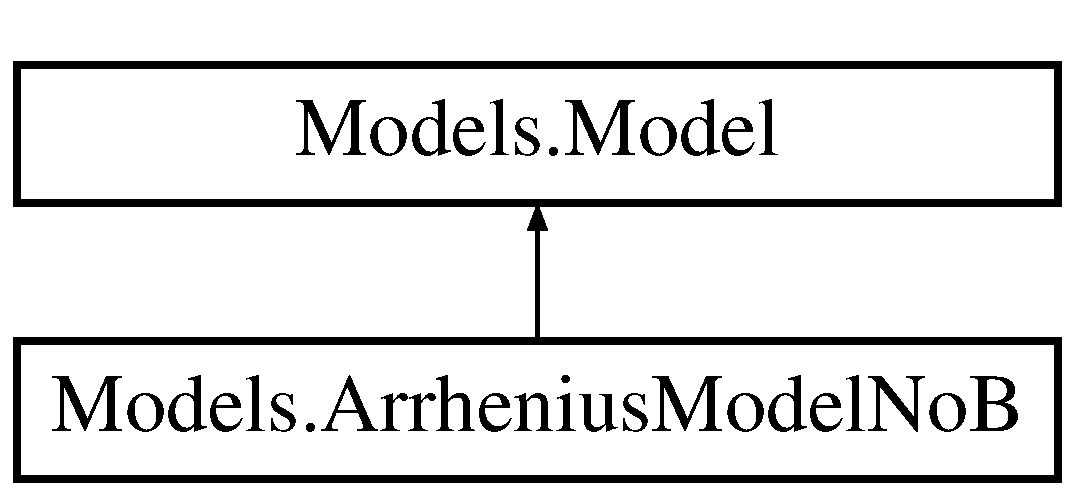
\includegraphics[height=2.000000cm]{classModels_1_1ArrheniusModelNoB}
\end{center}
\end{figure}
\subsection*{\-Public \-Member \-Functions}
\begin{DoxyCompactItemize}
\item 
\hypertarget{classModels_1_1ArrheniusModelNoB_ad0a055e1a0bd58308116136d54d16ffb}{def {\bfseries \-\_\-\-\_\-init\-\_\-\-\_\-}}\label{classModels_1_1ArrheniusModelNoB_ad0a055e1a0bd58308116136d54d16ffb}

\item 
def \hyperlink{classModels_1_1ArrheniusModelNoB_ad6e29a334e64d65beb7b0785b2979644}{calc\-Mass}
\item 
def \hyperlink{classModels_1_1ArrheniusModelNoB_a6c26a473f8e08dd6d6651dd0b7c7a8a5}{\-Convert\-Kin\-Factors}
\item 
def \hyperlink{classModels_1_1Model_a317ed848b969dbe3a96dd05e8b771900}{plt\-Yield}
\item 
def \hyperlink{classModels_1_1Model_aa35c741babf8f141df48c4021e0664e4}{plt\-Rate}
\item 
def \hyperlink{classModels_1_1Model_a3396d6ca1a7b7d66e55ada8c3c7a509e}{max\-Length\-Of\-Vectors}
\item 
def \hyperlink{classModels_1_1Model_ae404a691e48bfe4eafcdfdd09f1dae48}{plot}
\item 
def \hyperlink{classModels_1_1Model_a010945ed2adff59a7a5fce36025e7a97}{derive\-C}
\item 
def \hyperlink{classModels_1_1Model_a7c9280e33f9e0d46703cebc131008c65}{calc\-Rate}
\item 
def \hyperlink{classModels_1_1Model_a818f207e2a4bd0e9a3720ca611960e5a}{set\-Param\-Vector}
\item 
def \hyperlink{classModels_1_1Model_a13c76a0fe24d43cdc4d21fbc73fa96fa}{\-Param\-Vector}
\item 
def \hyperlink{classModels_1_1Model_ad3e627980d9e781bf7b2c9ff900ca06b}{\-Error\-Yield}
\item 
def \hyperlink{classModels_1_1Model_a3050eb39341f318d8d88b172f88bd240}{\-Error\-Rate}
\item 
def \hyperlink{classModels_1_1Model_adcb987bccae63a742490ea1e6d5f7a74}{mk\-Simple\-Result\-Files}
\item 
def \hyperlink{classModels_1_1Model_ac28252ae5cd6b5ecd4c5d006a0e6567d}{set\-Dt4\-Intergrate}
\end{DoxyCompactItemize}
\subsection*{\-Public \-Attributes}
\begin{DoxyCompactItemize}
\item 
\hypertarget{classModels_1_1ArrheniusModelNoB_a2d30c2c2ac26561a369e3378c3057bb4}{{\bfseries \-O\-D\-E\-\_\-hmax}}\label{classModels_1_1ArrheniusModelNoB_a2d30c2c2ac26561a369e3378c3057bb4}

\item 
\hypertarget{classModels_1_1ArrheniusModelNoB_afdf3d4c6cef8d0a613d4b99c936b136a}{{\bfseries const\-Dt}}\label{classModels_1_1ArrheniusModelNoB_afdf3d4c6cef8d0a613d4b99c936b136a}

\item 
\hypertarget{classModels_1_1Model_a3f71983de5f8b86bec47929213b900ec}{{\bfseries const\-Dt\-Vec}}\label{classModels_1_1Model_a3f71983de5f8b86bec47929213b900ec}

\end{DoxyCompactItemize}


\subsection{\-Detailed \-Description}
\begin{DoxyVerb}The Arrhenius model in the standart notation: dm/dt=A*exp(-E/T)*(m_s-m) with the parameter a,b,E to optimize.\end{DoxyVerb}
 

\subsection{\-Member \-Function \-Documentation}
\hypertarget{classModels_1_1ArrheniusModelNoB_ad6e29a334e64d65beb7b0785b2979644}{\index{\-Models\-::\-Arrhenius\-Model\-No\-B@{\-Models\-::\-Arrhenius\-Model\-No\-B}!calc\-Mass@{calc\-Mass}}
\index{calc\-Mass@{calc\-Mass}!Models::ArrheniusModelNoB@{\-Models\-::\-Arrhenius\-Model\-No\-B}}
\subsubsection[{calc\-Mass}]{\setlength{\rightskip}{0pt plus 5cm}def {\bf \-Models.\-Arrhenius\-Model\-No\-B.\-calc\-Mass} (
\begin{DoxyParamCaption}
\item[{}]{self, }
\item[{}]{fgdvc, }
\item[{}]{time, }
\item[{}]{\-T, }
\item[{}]{\-Name}
\end{DoxyParamCaption}
)}}\label{classModels_1_1ArrheniusModelNoB_ad6e29a334e64d65beb7b0785b2979644}
\begin{DoxyVerb}Outputs the mass(t) using the model specific equation.\end{DoxyVerb}
 \hypertarget{classModels_1_1Model_a7c9280e33f9e0d46703cebc131008c65}{\index{\-Models\-::\-Arrhenius\-Model\-No\-B@{\-Models\-::\-Arrhenius\-Model\-No\-B}!calc\-Rate@{calc\-Rate}}
\index{calc\-Rate@{calc\-Rate}!Models::ArrheniusModelNoB@{\-Models\-::\-Arrhenius\-Model\-No\-B}}
\subsubsection[{calc\-Rate}]{\setlength{\rightskip}{0pt plus 5cm}def {\bf \-Models.\-Model.\-calc\-Rate} (
\begin{DoxyParamCaption}
\item[{}]{self, }
\item[{}]{fgdvc, }
\item[{}]{time, }
\item[{}]{\-T, }
\item[{}]{\-Name}
\end{DoxyParamCaption}
)\hspace{0.3cm}{\ttfamily  \mbox{[}inherited\mbox{]}}}}\label{classModels_1_1Model_a7c9280e33f9e0d46703cebc131008c65}
\begin{DoxyVerb}Generates the Rates using the yields vector and a CDS.\end{DoxyVerb}
 \hypertarget{classModels_1_1ArrheniusModelNoB_a6c26a473f8e08dd6d6651dd0b7c7a8a5}{\index{\-Models\-::\-Arrhenius\-Model\-No\-B@{\-Models\-::\-Arrhenius\-Model\-No\-B}!\-Convert\-Kin\-Factors@{\-Convert\-Kin\-Factors}}
\index{\-Convert\-Kin\-Factors@{\-Convert\-Kin\-Factors}!Models::ArrheniusModelNoB@{\-Models\-::\-Arrhenius\-Model\-No\-B}}
\subsubsection[{\-Convert\-Kin\-Factors}]{\setlength{\rightskip}{0pt plus 5cm}def {\bf \-Models.\-Arrhenius\-Model\-No\-B.\-Convert\-Kin\-Factors} (
\begin{DoxyParamCaption}
\item[{}]{self, }
\item[{}]{\-Parameter\-Vector}
\end{DoxyParamCaption}
)}}\label{classModels_1_1ArrheniusModelNoB_a6c26a473f8e08dd6d6651dd0b7c7a8a5}
\begin{DoxyVerb}Dummy. Function actual has to convert the parameter into the standart Arrhenius notation.\end{DoxyVerb}
 \hypertarget{classModels_1_1Model_a010945ed2adff59a7a5fce36025e7a97}{\index{\-Models\-::\-Arrhenius\-Model\-No\-B@{\-Models\-::\-Arrhenius\-Model\-No\-B}!derive\-C@{derive\-C}}
\index{derive\-C@{derive\-C}!Models::ArrheniusModelNoB@{\-Models\-::\-Arrhenius\-Model\-No\-B}}
\subsubsection[{derive\-C}]{\setlength{\rightskip}{0pt plus 5cm}def {\bf \-Models.\-Model.\-derive\-C} (
\begin{DoxyParamCaption}
\item[{}]{self, }
\item[{}]{fgdvc, }
\item[{}]{y\-Vector}
\end{DoxyParamCaption}
)\hspace{0.3cm}{\ttfamily  \mbox{[}inherited\mbox{]}}}}\label{classModels_1_1Model_a010945ed2adff59a7a5fce36025e7a97}
\begin{DoxyVerb}Returns a CDS of the inputted yVector.\end{DoxyVerb}
 \hypertarget{classModels_1_1Model_a3050eb39341f318d8d88b172f88bd240}{\index{\-Models\-::\-Arrhenius\-Model\-No\-B@{\-Models\-::\-Arrhenius\-Model\-No\-B}!\-Error\-Rate@{\-Error\-Rate}}
\index{\-Error\-Rate@{\-Error\-Rate}!Models::ArrheniusModelNoB@{\-Models\-::\-Arrhenius\-Model\-No\-B}}
\subsubsection[{\-Error\-Rate}]{\setlength{\rightskip}{0pt plus 5cm}def {\bf \-Models.\-Model.\-Error\-Rate} (
\begin{DoxyParamCaption}
\item[{}]{self, }
\item[{}]{fgdvc, }
\item[{}]{\-Species}
\end{DoxyParamCaption}
)\hspace{0.3cm}{\ttfamily  \mbox{[}inherited\mbox{]}}}}\label{classModels_1_1Model_a3050eb39341f318d8d88b172f88bd240}
\begin{DoxyVerb}Returns the absolute deviation per point between the fitted and the original rate curve.\end{DoxyVerb}
 \hypertarget{classModels_1_1Model_ad3e627980d9e781bf7b2c9ff900ca06b}{\index{\-Models\-::\-Arrhenius\-Model\-No\-B@{\-Models\-::\-Arrhenius\-Model\-No\-B}!\-Error\-Yield@{\-Error\-Yield}}
\index{\-Error\-Yield@{\-Error\-Yield}!Models::ArrheniusModelNoB@{\-Models\-::\-Arrhenius\-Model\-No\-B}}
\subsubsection[{\-Error\-Yield}]{\setlength{\rightskip}{0pt plus 5cm}def {\bf \-Models.\-Model.\-Error\-Yield} (
\begin{DoxyParamCaption}
\item[{}]{self, }
\item[{}]{fgdvc, }
\item[{}]{\-Species}
\end{DoxyParamCaption}
)\hspace{0.3cm}{\ttfamily  \mbox{[}inherited\mbox{]}}}}\label{classModels_1_1Model_ad3e627980d9e781bf7b2c9ff900ca06b}
\begin{DoxyVerb}Returns the absolute deviation per point between the fitted and the original yield curve.\end{DoxyVerb}
 \hypertarget{classModels_1_1Model_a3396d6ca1a7b7d66e55ada8c3c7a509e}{\index{\-Models\-::\-Arrhenius\-Model\-No\-B@{\-Models\-::\-Arrhenius\-Model\-No\-B}!max\-Length\-Of\-Vectors@{max\-Length\-Of\-Vectors}}
\index{max\-Length\-Of\-Vectors@{max\-Length\-Of\-Vectors}!Models::ArrheniusModelNoB@{\-Models\-::\-Arrhenius\-Model\-No\-B}}
\subsubsection[{max\-Length\-Of\-Vectors}]{\setlength{\rightskip}{0pt plus 5cm}def {\bf \-Models.\-Model.\-max\-Length\-Of\-Vectors} (
\begin{DoxyParamCaption}
\item[{}]{self, }
\item[{}]{fgdvc\-\_\-list}
\end{DoxyParamCaption}
)\hspace{0.3cm}{\ttfamily  \mbox{[}inherited\mbox{]}}}}\label{classModels_1_1Model_a3396d6ca1a7b7d66e55ada8c3c7a509e}
\begin{DoxyVerb}Returns the minimum lenght of a all vectors from the several runs.\end{DoxyVerb}
 \hypertarget{classModels_1_1Model_adcb987bccae63a742490ea1e6d5f7a74}{\index{\-Models\-::\-Arrhenius\-Model\-No\-B@{\-Models\-::\-Arrhenius\-Model\-No\-B}!mk\-Simple\-Result\-Files@{mk\-Simple\-Result\-Files}}
\index{mk\-Simple\-Result\-Files@{mk\-Simple\-Result\-Files}!Models::ArrheniusModelNoB@{\-Models\-::\-Arrhenius\-Model\-No\-B}}
\subsubsection[{mk\-Simple\-Result\-Files}]{\setlength{\rightskip}{0pt plus 5cm}def {\bf \-Models.\-Model.\-mk\-Simple\-Result\-Files} (
\begin{DoxyParamCaption}
\item[{}]{self, }
\item[{}]{fgdvc\-\_\-list, }
\item[{}]{\-Species}
\end{DoxyParamCaption}
)\hspace{0.3cm}{\ttfamily  \mbox{[}inherited\mbox{]}}}}\label{classModels_1_1Model_adcb987bccae63a742490ea1e6d5f7a74}
\begin{DoxyVerb}Simple result file if no fitting is carried out. Writes only the transformed results into a file.\end{DoxyVerb}
 \hypertarget{classModels_1_1Model_a13c76a0fe24d43cdc4d21fbc73fa96fa}{\index{\-Models\-::\-Arrhenius\-Model\-No\-B@{\-Models\-::\-Arrhenius\-Model\-No\-B}!\-Param\-Vector@{\-Param\-Vector}}
\index{\-Param\-Vector@{\-Param\-Vector}!Models::ArrheniusModelNoB@{\-Models\-::\-Arrhenius\-Model\-No\-B}}
\subsubsection[{\-Param\-Vector}]{\setlength{\rightskip}{0pt plus 5cm}def {\bf \-Models.\-Model.\-Param\-Vector} (
\begin{DoxyParamCaption}
\item[{}]{self}
\end{DoxyParamCaption}
)\hspace{0.3cm}{\ttfamily  \mbox{[}inherited\mbox{]}}}}\label{classModels_1_1Model_a13c76a0fe24d43cdc4d21fbc73fa96fa}
\begin{DoxyVerb}Returns the Vector containing the kinetic parameter of the Model (refering to the child model).\end{DoxyVerb}
 \hypertarget{classModels_1_1Model_ae404a691e48bfe4eafcdfdd09f1dae48}{\index{\-Models\-::\-Arrhenius\-Model\-No\-B@{\-Models\-::\-Arrhenius\-Model\-No\-B}!plot@{plot}}
\index{plot@{plot}!Models::ArrheniusModelNoB@{\-Models\-::\-Arrhenius\-Model\-No\-B}}
\subsubsection[{plot}]{\setlength{\rightskip}{0pt plus 5cm}def {\bf \-Models.\-Model.\-plot} (
\begin{DoxyParamCaption}
\item[{}]{self, }
\item[{}]{fgdvc\-\_\-list, }
\item[{}]{\-Species}
\end{DoxyParamCaption}
)\hspace{0.3cm}{\ttfamily  \mbox{[}inherited\mbox{]}}}}\label{classModels_1_1Model_ae404a691e48bfe4eafcdfdd09f1dae48}
\begin{DoxyVerb}Plot the yield and the rates over time with two curves: one is the original data, the other the fitting curve. Also file 'PyrolysisProgramName-Species.out' (e.g. 'CPD-CO2.out') containing the time (s), yields (kg/kg), rates (kg/(kg s)).\end{DoxyVerb}
 \hypertarget{classModels_1_1Model_aa35c741babf8f141df48c4021e0664e4}{\index{\-Models\-::\-Arrhenius\-Model\-No\-B@{\-Models\-::\-Arrhenius\-Model\-No\-B}!plt\-Rate@{plt\-Rate}}
\index{plt\-Rate@{plt\-Rate}!Models::ArrheniusModelNoB@{\-Models\-::\-Arrhenius\-Model\-No\-B}}
\subsubsection[{plt\-Rate}]{\setlength{\rightskip}{0pt plus 5cm}def {\bf \-Models.\-Model.\-plt\-Rate} (
\begin{DoxyParamCaption}
\item[{}]{self, }
\item[{}]{fgdvc\-\_\-list, }
\item[{}]{x\-Value\-To\-Plot, }
\item[{}]{y\-Value\-To\-Plot}
\end{DoxyParamCaption}
)\hspace{0.3cm}{\ttfamily  \mbox{[}inherited\mbox{]}}}}\label{classModels_1_1Model_aa35c741babf8f141df48c4021e0664e4}
\begin{DoxyVerb}Plots the rates (to select with yValueToPlot) over Time or Temperature (to slect with xValueToPlot).\end{DoxyVerb}
 \hypertarget{classModels_1_1Model_a317ed848b969dbe3a96dd05e8b771900}{\index{\-Models\-::\-Arrhenius\-Model\-No\-B@{\-Models\-::\-Arrhenius\-Model\-No\-B}!plt\-Yield@{plt\-Yield}}
\index{plt\-Yield@{plt\-Yield}!Models::ArrheniusModelNoB@{\-Models\-::\-Arrhenius\-Model\-No\-B}}
\subsubsection[{plt\-Yield}]{\setlength{\rightskip}{0pt plus 5cm}def {\bf \-Models.\-Model.\-plt\-Yield} (
\begin{DoxyParamCaption}
\item[{}]{self, }
\item[{}]{fgdvc\-\_\-list, }
\item[{}]{x\-Value\-To\-Plot, }
\item[{}]{y\-Value\-To\-Plot}
\end{DoxyParamCaption}
)\hspace{0.3cm}{\ttfamily  \mbox{[}inherited\mbox{]}}}}\label{classModels_1_1Model_a317ed848b969dbe3a96dd05e8b771900}
\begin{DoxyVerb}Plots the yields (to select with yValueToPlot) over Time or Temperature (to slect with xValueToPlot).\end{DoxyVerb}
 \hypertarget{classModels_1_1Model_ac28252ae5cd6b5ecd4c5d006a0e6567d}{\index{\-Models\-::\-Arrhenius\-Model\-No\-B@{\-Models\-::\-Arrhenius\-Model\-No\-B}!set\-Dt4\-Intergrate@{set\-Dt4\-Intergrate}}
\index{set\-Dt4\-Intergrate@{set\-Dt4\-Intergrate}!Models::ArrheniusModelNoB@{\-Models\-::\-Arrhenius\-Model\-No\-B}}
\subsubsection[{set\-Dt4\-Intergrate}]{\setlength{\rightskip}{0pt plus 5cm}def {\bf \-Models.\-Model.\-set\-Dt4\-Intergrate} (
\begin{DoxyParamCaption}
\item[{}]{self, }
\item[{}]{constant\-Dt}
\end{DoxyParamCaption}
)\hspace{0.3cm}{\ttfamily  \mbox{[}inherited\mbox{]}}}}\label{classModels_1_1Model_ac28252ae5cd6b5ecd4c5d006a0e6567d}
\begin{DoxyVerb}constantDt allows the option to define numerical time step to solve the ODE. The outputted results ever equal the imported time list (when applying method calcMass Time = [t0,t1,t2,t3,t4]. If these time steps are too large, then is this defined dt used to solve the ODE and the results are linear interploated that way that they correspond to the imported time vector. To reset it, just set constantDt to False.\end{DoxyVerb}
 \hypertarget{classModels_1_1Model_a818f207e2a4bd0e9a3720ca611960e5a}{\index{\-Models\-::\-Arrhenius\-Model\-No\-B@{\-Models\-::\-Arrhenius\-Model\-No\-B}!set\-Param\-Vector@{set\-Param\-Vector}}
\index{set\-Param\-Vector@{set\-Param\-Vector}!Models::ArrheniusModelNoB@{\-Models\-::\-Arrhenius\-Model\-No\-B}}
\subsubsection[{set\-Param\-Vector}]{\setlength{\rightskip}{0pt plus 5cm}def {\bf \-Models.\-Model.\-set\-Param\-Vector} (
\begin{DoxyParamCaption}
\item[{}]{self, }
\item[{}]{\-Parameter\-List}
\end{DoxyParamCaption}
)\hspace{0.3cm}{\ttfamily  \mbox{[}inherited\mbox{]}}}}\label{classModels_1_1Model_a818f207e2a4bd0e9a3720ca611960e5a}
\begin{DoxyVerb}Sets the Vector containing the kinetic parameter of the Model (refering to the child model).\end{DoxyVerb}
 

\-The documentation for this class was generated from the following file\-:\begin{DoxyCompactItemize}
\item 
/home/map/git/pkp/src/\-Models.\-py\end{DoxyCompactItemize}

\hypertarget{classModels_1_1ConstantRateModel}{\section{\-Models.\-Constant\-Rate\-Model \-Class \-Reference}
\label{classModels_1_1ConstantRateModel}\index{\-Models.\-Constant\-Rate\-Model@{\-Models.\-Constant\-Rate\-Model}}
}
\-Inheritance diagram for \-Models.\-Constant\-Rate\-Model\-:\begin{figure}[H]
\begin{center}
\leavevmode
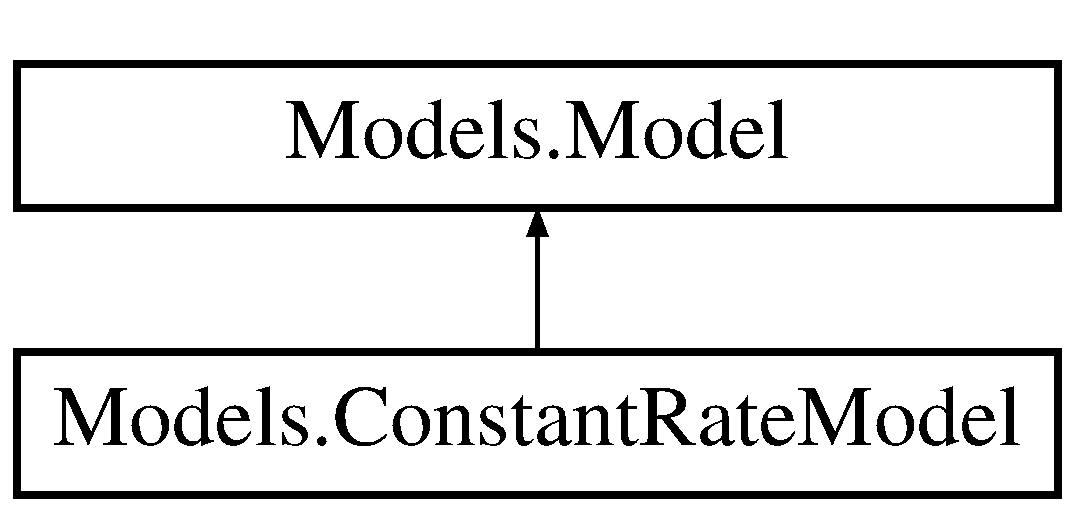
\includegraphics[height=2.000000cm]{classModels_1_1ConstantRateModel}
\end{center}
\end{figure}
\subsection*{\-Public \-Member \-Functions}
\begin{DoxyCompactItemize}
\item 
\hypertarget{classModels_1_1ConstantRateModel_a1dbc868c3fea6eb4e2de48c26ca28d21}{def {\bfseries \-\_\-\-\_\-init\-\_\-\-\_\-}}\label{classModels_1_1ConstantRateModel_a1dbc868c3fea6eb4e2de48c26ca28d21}

\item 
\hypertarget{classModels_1_1ConstantRateModel_adda655b4249b8e737d08c51c962165f1}{def {\bfseries calc\-Mass}}\label{classModels_1_1ConstantRateModel_adda655b4249b8e737d08c51c962165f1}

\item 
def \hyperlink{classModels_1_1Model_a317ed848b969dbe3a96dd05e8b771900}{plt\-Yield}
\item 
def \hyperlink{classModels_1_1Model_aa35c741babf8f141df48c4021e0664e4}{plt\-Rate}
\item 
def \hyperlink{classModels_1_1Model_a3396d6ca1a7b7d66e55ada8c3c7a509e}{max\-Length\-Of\-Vectors}
\item 
def \hyperlink{classModels_1_1Model_ae404a691e48bfe4eafcdfdd09f1dae48}{plot}
\item 
def \hyperlink{classModels_1_1Model_a010945ed2adff59a7a5fce36025e7a97}{derive\-C}
\item 
def \hyperlink{classModels_1_1Model_a7c9280e33f9e0d46703cebc131008c65}{calc\-Rate}
\item 
def \hyperlink{classModels_1_1Model_a818f207e2a4bd0e9a3720ca611960e5a}{set\-Param\-Vector}
\item 
def \hyperlink{classModels_1_1Model_a13c76a0fe24d43cdc4d21fbc73fa96fa}{\-Param\-Vector}
\item 
def \hyperlink{classModels_1_1Model_ad3e627980d9e781bf7b2c9ff900ca06b}{\-Error\-Yield}
\item 
def \hyperlink{classModels_1_1Model_a3050eb39341f318d8d88b172f88bd240}{\-Error\-Rate}
\item 
def \hyperlink{classModels_1_1Model_adcb987bccae63a742490ea1e6d5f7a74}{mk\-Simple\-Result\-Files}
\item 
def \hyperlink{classModels_1_1Model_ac28252ae5cd6b5ecd4c5d006a0e6567d}{set\-Dt4\-Intergrate}
\end{DoxyCompactItemize}
\subsection*{\-Public \-Attributes}
\begin{DoxyCompactItemize}
\item 
\hypertarget{classModels_1_1ConstantRateModel_ac6e5d7c5f8ee942649b6a532d5bb45b7}{{\bfseries const\-Dt}}\label{classModels_1_1ConstantRateModel_ac6e5d7c5f8ee942649b6a532d5bb45b7}

\item 
\hypertarget{classModels_1_1Model_a3f71983de5f8b86bec47929213b900ec}{{\bfseries const\-Dt\-Vec}}\label{classModels_1_1Model_a3f71983de5f8b86bec47929213b900ec}

\end{DoxyCompactItemize}


\subsection{\-Detailed \-Description}
\begin{DoxyVerb}The model calculating the mass with m(t)=m_s0+(m_s0-m_s,e)*e**(-k*(t-t_start)) from the ODE dm/dt = -k*(m-m_s,e). The Parameter to optimize are k and t_start.\end{DoxyVerb}
 

\subsection{\-Member \-Function \-Documentation}
\hypertarget{classModels_1_1Model_a7c9280e33f9e0d46703cebc131008c65}{\index{\-Models\-::\-Constant\-Rate\-Model@{\-Models\-::\-Constant\-Rate\-Model}!calc\-Rate@{calc\-Rate}}
\index{calc\-Rate@{calc\-Rate}!Models::ConstantRateModel@{\-Models\-::\-Constant\-Rate\-Model}}
\subsubsection[{calc\-Rate}]{\setlength{\rightskip}{0pt plus 5cm}def {\bf \-Models.\-Model.\-calc\-Rate} (
\begin{DoxyParamCaption}
\item[{}]{self, }
\item[{}]{fgdvc, }
\item[{}]{time, }
\item[{}]{\-T, }
\item[{}]{\-Name}
\end{DoxyParamCaption}
)\hspace{0.3cm}{\ttfamily  \mbox{[}inherited\mbox{]}}}}\label{classModels_1_1Model_a7c9280e33f9e0d46703cebc131008c65}
\begin{DoxyVerb}Generates the Rates using the yields vector and a CDS.\end{DoxyVerb}
 \hypertarget{classModels_1_1Model_a010945ed2adff59a7a5fce36025e7a97}{\index{\-Models\-::\-Constant\-Rate\-Model@{\-Models\-::\-Constant\-Rate\-Model}!derive\-C@{derive\-C}}
\index{derive\-C@{derive\-C}!Models::ConstantRateModel@{\-Models\-::\-Constant\-Rate\-Model}}
\subsubsection[{derive\-C}]{\setlength{\rightskip}{0pt plus 5cm}def {\bf \-Models.\-Model.\-derive\-C} (
\begin{DoxyParamCaption}
\item[{}]{self, }
\item[{}]{fgdvc, }
\item[{}]{y\-Vector}
\end{DoxyParamCaption}
)\hspace{0.3cm}{\ttfamily  \mbox{[}inherited\mbox{]}}}}\label{classModels_1_1Model_a010945ed2adff59a7a5fce36025e7a97}
\begin{DoxyVerb}Returns a CDS of the inputted yVector.\end{DoxyVerb}
 \hypertarget{classModels_1_1Model_a3050eb39341f318d8d88b172f88bd240}{\index{\-Models\-::\-Constant\-Rate\-Model@{\-Models\-::\-Constant\-Rate\-Model}!\-Error\-Rate@{\-Error\-Rate}}
\index{\-Error\-Rate@{\-Error\-Rate}!Models::ConstantRateModel@{\-Models\-::\-Constant\-Rate\-Model}}
\subsubsection[{\-Error\-Rate}]{\setlength{\rightskip}{0pt plus 5cm}def {\bf \-Models.\-Model.\-Error\-Rate} (
\begin{DoxyParamCaption}
\item[{}]{self, }
\item[{}]{fgdvc, }
\item[{}]{\-Species}
\end{DoxyParamCaption}
)\hspace{0.3cm}{\ttfamily  \mbox{[}inherited\mbox{]}}}}\label{classModels_1_1Model_a3050eb39341f318d8d88b172f88bd240}
\begin{DoxyVerb}Returns the absolute deviation per point between the fitted and the original rate curve.\end{DoxyVerb}
 \hypertarget{classModels_1_1Model_ad3e627980d9e781bf7b2c9ff900ca06b}{\index{\-Models\-::\-Constant\-Rate\-Model@{\-Models\-::\-Constant\-Rate\-Model}!\-Error\-Yield@{\-Error\-Yield}}
\index{\-Error\-Yield@{\-Error\-Yield}!Models::ConstantRateModel@{\-Models\-::\-Constant\-Rate\-Model}}
\subsubsection[{\-Error\-Yield}]{\setlength{\rightskip}{0pt plus 5cm}def {\bf \-Models.\-Model.\-Error\-Yield} (
\begin{DoxyParamCaption}
\item[{}]{self, }
\item[{}]{fgdvc, }
\item[{}]{\-Species}
\end{DoxyParamCaption}
)\hspace{0.3cm}{\ttfamily  \mbox{[}inherited\mbox{]}}}}\label{classModels_1_1Model_ad3e627980d9e781bf7b2c9ff900ca06b}
\begin{DoxyVerb}Returns the absolute deviation per point between the fitted and the original yield curve.\end{DoxyVerb}
 \hypertarget{classModels_1_1Model_a3396d6ca1a7b7d66e55ada8c3c7a509e}{\index{\-Models\-::\-Constant\-Rate\-Model@{\-Models\-::\-Constant\-Rate\-Model}!max\-Length\-Of\-Vectors@{max\-Length\-Of\-Vectors}}
\index{max\-Length\-Of\-Vectors@{max\-Length\-Of\-Vectors}!Models::ConstantRateModel@{\-Models\-::\-Constant\-Rate\-Model}}
\subsubsection[{max\-Length\-Of\-Vectors}]{\setlength{\rightskip}{0pt plus 5cm}def {\bf \-Models.\-Model.\-max\-Length\-Of\-Vectors} (
\begin{DoxyParamCaption}
\item[{}]{self, }
\item[{}]{fgdvc\-\_\-list}
\end{DoxyParamCaption}
)\hspace{0.3cm}{\ttfamily  \mbox{[}inherited\mbox{]}}}}\label{classModels_1_1Model_a3396d6ca1a7b7d66e55ada8c3c7a509e}
\begin{DoxyVerb}Returns the minimum lenght of a all vectors from the several runs.\end{DoxyVerb}
 \hypertarget{classModels_1_1Model_adcb987bccae63a742490ea1e6d5f7a74}{\index{\-Models\-::\-Constant\-Rate\-Model@{\-Models\-::\-Constant\-Rate\-Model}!mk\-Simple\-Result\-Files@{mk\-Simple\-Result\-Files}}
\index{mk\-Simple\-Result\-Files@{mk\-Simple\-Result\-Files}!Models::ConstantRateModel@{\-Models\-::\-Constant\-Rate\-Model}}
\subsubsection[{mk\-Simple\-Result\-Files}]{\setlength{\rightskip}{0pt plus 5cm}def {\bf \-Models.\-Model.\-mk\-Simple\-Result\-Files} (
\begin{DoxyParamCaption}
\item[{}]{self, }
\item[{}]{fgdvc\-\_\-list, }
\item[{}]{\-Species}
\end{DoxyParamCaption}
)\hspace{0.3cm}{\ttfamily  \mbox{[}inherited\mbox{]}}}}\label{classModels_1_1Model_adcb987bccae63a742490ea1e6d5f7a74}
\begin{DoxyVerb}Simple result file if no fitting is carried out. Writes only the transformed results into a file.\end{DoxyVerb}
 \hypertarget{classModels_1_1Model_a13c76a0fe24d43cdc4d21fbc73fa96fa}{\index{\-Models\-::\-Constant\-Rate\-Model@{\-Models\-::\-Constant\-Rate\-Model}!\-Param\-Vector@{\-Param\-Vector}}
\index{\-Param\-Vector@{\-Param\-Vector}!Models::ConstantRateModel@{\-Models\-::\-Constant\-Rate\-Model}}
\subsubsection[{\-Param\-Vector}]{\setlength{\rightskip}{0pt plus 5cm}def {\bf \-Models.\-Model.\-Param\-Vector} (
\begin{DoxyParamCaption}
\item[{}]{self}
\end{DoxyParamCaption}
)\hspace{0.3cm}{\ttfamily  \mbox{[}inherited\mbox{]}}}}\label{classModels_1_1Model_a13c76a0fe24d43cdc4d21fbc73fa96fa}
\begin{DoxyVerb}Returns the Vector containing the kinetic parameter of the Model (refering to the child model).\end{DoxyVerb}
 \hypertarget{classModels_1_1Model_ae404a691e48bfe4eafcdfdd09f1dae48}{\index{\-Models\-::\-Constant\-Rate\-Model@{\-Models\-::\-Constant\-Rate\-Model}!plot@{plot}}
\index{plot@{plot}!Models::ConstantRateModel@{\-Models\-::\-Constant\-Rate\-Model}}
\subsubsection[{plot}]{\setlength{\rightskip}{0pt plus 5cm}def {\bf \-Models.\-Model.\-plot} (
\begin{DoxyParamCaption}
\item[{}]{self, }
\item[{}]{fgdvc\-\_\-list, }
\item[{}]{\-Species}
\end{DoxyParamCaption}
)\hspace{0.3cm}{\ttfamily  \mbox{[}inherited\mbox{]}}}}\label{classModels_1_1Model_ae404a691e48bfe4eafcdfdd09f1dae48}
\begin{DoxyVerb}Plot the yield and the rates over time with two curves: one is the original data, the other the fitting curve. Also file 'PyrolysisProgramName-Species.out' (e.g. 'CPD-CO2.out') containing the time (s), yields (kg/kg), rates (kg/(kg s)).\end{DoxyVerb}
 \hypertarget{classModels_1_1Model_aa35c741babf8f141df48c4021e0664e4}{\index{\-Models\-::\-Constant\-Rate\-Model@{\-Models\-::\-Constant\-Rate\-Model}!plt\-Rate@{plt\-Rate}}
\index{plt\-Rate@{plt\-Rate}!Models::ConstantRateModel@{\-Models\-::\-Constant\-Rate\-Model}}
\subsubsection[{plt\-Rate}]{\setlength{\rightskip}{0pt plus 5cm}def {\bf \-Models.\-Model.\-plt\-Rate} (
\begin{DoxyParamCaption}
\item[{}]{self, }
\item[{}]{fgdvc\-\_\-list, }
\item[{}]{x\-Value\-To\-Plot, }
\item[{}]{y\-Value\-To\-Plot}
\end{DoxyParamCaption}
)\hspace{0.3cm}{\ttfamily  \mbox{[}inherited\mbox{]}}}}\label{classModels_1_1Model_aa35c741babf8f141df48c4021e0664e4}
\begin{DoxyVerb}Plots the rates (to select with yValueToPlot) over Time or Temperature (to slect with xValueToPlot).\end{DoxyVerb}
 \hypertarget{classModels_1_1Model_a317ed848b969dbe3a96dd05e8b771900}{\index{\-Models\-::\-Constant\-Rate\-Model@{\-Models\-::\-Constant\-Rate\-Model}!plt\-Yield@{plt\-Yield}}
\index{plt\-Yield@{plt\-Yield}!Models::ConstantRateModel@{\-Models\-::\-Constant\-Rate\-Model}}
\subsubsection[{plt\-Yield}]{\setlength{\rightskip}{0pt plus 5cm}def {\bf \-Models.\-Model.\-plt\-Yield} (
\begin{DoxyParamCaption}
\item[{}]{self, }
\item[{}]{fgdvc\-\_\-list, }
\item[{}]{x\-Value\-To\-Plot, }
\item[{}]{y\-Value\-To\-Plot}
\end{DoxyParamCaption}
)\hspace{0.3cm}{\ttfamily  \mbox{[}inherited\mbox{]}}}}\label{classModels_1_1Model_a317ed848b969dbe3a96dd05e8b771900}
\begin{DoxyVerb}Plots the yields (to select with yValueToPlot) over Time or Temperature (to slect with xValueToPlot).\end{DoxyVerb}
 \hypertarget{classModels_1_1Model_ac28252ae5cd6b5ecd4c5d006a0e6567d}{\index{\-Models\-::\-Constant\-Rate\-Model@{\-Models\-::\-Constant\-Rate\-Model}!set\-Dt4\-Intergrate@{set\-Dt4\-Intergrate}}
\index{set\-Dt4\-Intergrate@{set\-Dt4\-Intergrate}!Models::ConstantRateModel@{\-Models\-::\-Constant\-Rate\-Model}}
\subsubsection[{set\-Dt4\-Intergrate}]{\setlength{\rightskip}{0pt plus 5cm}def {\bf \-Models.\-Model.\-set\-Dt4\-Intergrate} (
\begin{DoxyParamCaption}
\item[{}]{self, }
\item[{}]{constant\-Dt}
\end{DoxyParamCaption}
)\hspace{0.3cm}{\ttfamily  \mbox{[}inherited\mbox{]}}}}\label{classModels_1_1Model_ac28252ae5cd6b5ecd4c5d006a0e6567d}
\begin{DoxyVerb}constantDt allows the option to define numerical time step to solve the ODE. The outputted results ever equal the imported time list (when applying method calcMass Time = [t0,t1,t2,t3,t4]. If these time steps are too large, then is this defined dt used to solve the ODE and the results are linear interploated that way that they correspond to the imported time vector. To reset it, just set constantDt to False.\end{DoxyVerb}
 \hypertarget{classModels_1_1Model_a818f207e2a4bd0e9a3720ca611960e5a}{\index{\-Models\-::\-Constant\-Rate\-Model@{\-Models\-::\-Constant\-Rate\-Model}!set\-Param\-Vector@{set\-Param\-Vector}}
\index{set\-Param\-Vector@{set\-Param\-Vector}!Models::ConstantRateModel@{\-Models\-::\-Constant\-Rate\-Model}}
\subsubsection[{set\-Param\-Vector}]{\setlength{\rightskip}{0pt plus 5cm}def {\bf \-Models.\-Model.\-set\-Param\-Vector} (
\begin{DoxyParamCaption}
\item[{}]{self, }
\item[{}]{\-Parameter\-List}
\end{DoxyParamCaption}
)\hspace{0.3cm}{\ttfamily  \mbox{[}inherited\mbox{]}}}}\label{classModels_1_1Model_a818f207e2a4bd0e9a3720ca611960e5a}
\begin{DoxyVerb}Sets the Vector containing the kinetic parameter of the Model (refering to the child model).\end{DoxyVerb}
 

\-The documentation for this class was generated from the following file\-:\begin{DoxyCompactItemize}
\item 
/home/map/git/pkp/src/\-Models.\-py\end{DoxyCompactItemize}

\hypertarget{classFit__one__run_1_1ConstantRateModel}{\section{\-Fit\-\_\-one\-\_\-run.\-Constant\-Rate\-Model \-Class \-Reference}
\label{classFit__one__run_1_1ConstantRateModel}\index{\-Fit\-\_\-one\-\_\-run.\-Constant\-Rate\-Model@{\-Fit\-\_\-one\-\_\-run.\-Constant\-Rate\-Model}}
}
\-Inheritance diagram for \-Fit\-\_\-one\-\_\-run.\-Constant\-Rate\-Model\-:\begin{figure}[H]
\begin{center}
\leavevmode
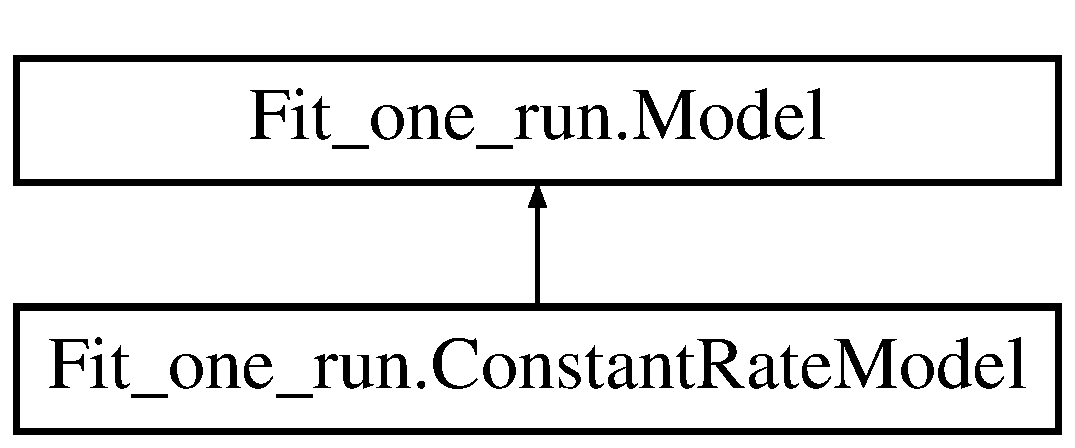
\includegraphics[height=2.000000cm]{classFit__one__run_1_1ConstantRateModel}
\end{center}
\end{figure}
\subsection*{\-Public \-Member \-Functions}
\begin{DoxyCompactItemize}
\item 
\hypertarget{classFit__one__run_1_1ConstantRateModel_a84c0d6f00d5e12e46e96ec406c4da10b}{def {\bfseries \-\_\-\-\_\-init\-\_\-\-\_\-}}\label{classFit__one__run_1_1ConstantRateModel_a84c0d6f00d5e12e46e96ec406c4da10b}

\item 
\hypertarget{classFit__one__run_1_1ConstantRateModel_aea8329a6ea8bb58312eeac92fa36ea28}{def {\bfseries calc\-Mass}}\label{classFit__one__run_1_1ConstantRateModel_aea8329a6ea8bb58312eeac92fa36ea28}

\item 
def \hyperlink{classFit__one__run_1_1Model_aa304b32155938a713c33f0dc03a135f3}{plt\-Yield}
\item 
def \hyperlink{classFit__one__run_1_1Model_a9c28d95902adf00f5aaa642f0919fc61}{plt\-Rate}
\item 
def \hyperlink{classFit__one__run_1_1Model_a26fc879ca33c9171ebb4a97bc4b0c46b}{min\-Length\-Of\-Vectors}
\item 
def \hyperlink{classFit__one__run_1_1Model_a98159c954f1f1be2a34be3ea53d11493}{plot}
\item 
def \hyperlink{classFit__one__run_1_1Model_ace9df4177c5ae753dbe190e2f8268149}{derive\-C}
\item 
def \hyperlink{classFit__one__run_1_1Model_a07ae4534de2a6ef241d71facdffb227e}{calc\-Rate}
\item 
def \hyperlink{classFit__one__run_1_1Model_a174aec9b05dbe01ec103f7ba75d6516c}{set\-Param\-Vector}
\item 
def \hyperlink{classFit__one__run_1_1Model_a3c9239f0ac062fdae0bda395636c0372}{\-Param\-Vector}
\item 
def \hyperlink{classFit__one__run_1_1Model_aa2bc4ba19704350fb2ff441734b51b10}{\-Error\-Yield}
\item 
def \hyperlink{classFit__one__run_1_1Model_aad63c345c343f0c7d1cf20135dc0a0e5}{\-Error\-Rate}
\end{DoxyCompactItemize}


\subsection{\-Detailed \-Description}
\begin{DoxyVerb}The model calculating the mass with m(t)=m_s0+(m_s0-m_s,e)*e**(-k*(t-t_start)) from the ODE dm/dt = -k*(m-m_s,e). The Parameter to optimize are k and t_start.\end{DoxyVerb}
 

\subsection{\-Member \-Function \-Documentation}
\hypertarget{classFit__one__run_1_1Model_a07ae4534de2a6ef241d71facdffb227e}{\index{\-Fit\-\_\-one\-\_\-run\-::\-Constant\-Rate\-Model@{\-Fit\-\_\-one\-\_\-run\-::\-Constant\-Rate\-Model}!calc\-Rate@{calc\-Rate}}
\index{calc\-Rate@{calc\-Rate}!Fit_one_run::ConstantRateModel@{\-Fit\-\_\-one\-\_\-run\-::\-Constant\-Rate\-Model}}
\subsubsection[{calc\-Rate}]{\setlength{\rightskip}{0pt plus 5cm}def {\bf \-Fit\-\_\-one\-\_\-run.\-Model.\-calc\-Rate} (
\begin{DoxyParamCaption}
\item[{}]{self, }
\item[{}]{fgdvc, }
\item[{}]{time, }
\item[{}]{\-T, }
\item[{}]{\-Name}
\end{DoxyParamCaption}
)\hspace{0.3cm}{\ttfamily  \mbox{[}inherited\mbox{]}}}}\label{classFit__one__run_1_1Model_a07ae4534de2a6ef241d71facdffb227e}
\begin{DoxyVerb}Generates the Rates using the yields vector and a CDS.\end{DoxyVerb}
 \hypertarget{classFit__one__run_1_1Model_ace9df4177c5ae753dbe190e2f8268149}{\index{\-Fit\-\_\-one\-\_\-run\-::\-Constant\-Rate\-Model@{\-Fit\-\_\-one\-\_\-run\-::\-Constant\-Rate\-Model}!derive\-C@{derive\-C}}
\index{derive\-C@{derive\-C}!Fit_one_run::ConstantRateModel@{\-Fit\-\_\-one\-\_\-run\-::\-Constant\-Rate\-Model}}
\subsubsection[{derive\-C}]{\setlength{\rightskip}{0pt plus 5cm}def {\bf \-Fit\-\_\-one\-\_\-run.\-Model.\-derive\-C} (
\begin{DoxyParamCaption}
\item[{}]{self, }
\item[{}]{fgdvc, }
\item[{}]{y\-Vector, }
\item[{}]{max\-Vector\-Lenght = {\ttfamily \-None}}
\end{DoxyParamCaption}
)\hspace{0.3cm}{\ttfamily  \mbox{[}inherited\mbox{]}}}}\label{classFit__one__run_1_1Model_ace9df4177c5ae753dbe190e2f8268149}
\begin{DoxyVerb}Returns a CDS of the inputted yVector.\end{DoxyVerb}
 \hypertarget{classFit__one__run_1_1Model_aad63c345c343f0c7d1cf20135dc0a0e5}{\index{\-Fit\-\_\-one\-\_\-run\-::\-Constant\-Rate\-Model@{\-Fit\-\_\-one\-\_\-run\-::\-Constant\-Rate\-Model}!\-Error\-Rate@{\-Error\-Rate}}
\index{\-Error\-Rate@{\-Error\-Rate}!Fit_one_run::ConstantRateModel@{\-Fit\-\_\-one\-\_\-run\-::\-Constant\-Rate\-Model}}
\subsubsection[{\-Error\-Rate}]{\setlength{\rightskip}{0pt plus 5cm}def {\bf \-Fit\-\_\-one\-\_\-run.\-Model.\-Error\-Rate} (
\begin{DoxyParamCaption}
\item[{}]{self, }
\item[{}]{fgdvc, }
\item[{}]{\-Species}
\end{DoxyParamCaption}
)\hspace{0.3cm}{\ttfamily  \mbox{[}inherited\mbox{]}}}}\label{classFit__one__run_1_1Model_aad63c345c343f0c7d1cf20135dc0a0e5}
\begin{DoxyVerb}Returns the absolute deviation per point between the fitted and the original rate curve.\end{DoxyVerb}
 \hypertarget{classFit__one__run_1_1Model_aa2bc4ba19704350fb2ff441734b51b10}{\index{\-Fit\-\_\-one\-\_\-run\-::\-Constant\-Rate\-Model@{\-Fit\-\_\-one\-\_\-run\-::\-Constant\-Rate\-Model}!\-Error\-Yield@{\-Error\-Yield}}
\index{\-Error\-Yield@{\-Error\-Yield}!Fit_one_run::ConstantRateModel@{\-Fit\-\_\-one\-\_\-run\-::\-Constant\-Rate\-Model}}
\subsubsection[{\-Error\-Yield}]{\setlength{\rightskip}{0pt plus 5cm}def {\bf \-Fit\-\_\-one\-\_\-run.\-Model.\-Error\-Yield} (
\begin{DoxyParamCaption}
\item[{}]{self, }
\item[{}]{fgdvc, }
\item[{}]{\-Species}
\end{DoxyParamCaption}
)\hspace{0.3cm}{\ttfamily  \mbox{[}inherited\mbox{]}}}}\label{classFit__one__run_1_1Model_aa2bc4ba19704350fb2ff441734b51b10}
\begin{DoxyVerb}Returns the absolute deviation per point between the fitted and the original yield curve.\end{DoxyVerb}
 \hypertarget{classFit__one__run_1_1Model_a26fc879ca33c9171ebb4a97bc4b0c46b}{\index{\-Fit\-\_\-one\-\_\-run\-::\-Constant\-Rate\-Model@{\-Fit\-\_\-one\-\_\-run\-::\-Constant\-Rate\-Model}!min\-Length\-Of\-Vectors@{min\-Length\-Of\-Vectors}}
\index{min\-Length\-Of\-Vectors@{min\-Length\-Of\-Vectors}!Fit_one_run::ConstantRateModel@{\-Fit\-\_\-one\-\_\-run\-::\-Constant\-Rate\-Model}}
\subsubsection[{min\-Length\-Of\-Vectors}]{\setlength{\rightskip}{0pt plus 5cm}def {\bf \-Fit\-\_\-one\-\_\-run.\-Model.\-min\-Length\-Of\-Vectors} (
\begin{DoxyParamCaption}
\item[{}]{self, }
\item[{}]{fgdvc\-\_\-list}
\end{DoxyParamCaption}
)\hspace{0.3cm}{\ttfamily  \mbox{[}inherited\mbox{]}}}}\label{classFit__one__run_1_1Model_a26fc879ca33c9171ebb4a97bc4b0c46b}
\begin{DoxyVerb}Returns the minimum lenght of a all vectors from the several runs.\end{DoxyVerb}
 \hypertarget{classFit__one__run_1_1Model_a3c9239f0ac062fdae0bda395636c0372}{\index{\-Fit\-\_\-one\-\_\-run\-::\-Constant\-Rate\-Model@{\-Fit\-\_\-one\-\_\-run\-::\-Constant\-Rate\-Model}!\-Param\-Vector@{\-Param\-Vector}}
\index{\-Param\-Vector@{\-Param\-Vector}!Fit_one_run::ConstantRateModel@{\-Fit\-\_\-one\-\_\-run\-::\-Constant\-Rate\-Model}}
\subsubsection[{\-Param\-Vector}]{\setlength{\rightskip}{0pt plus 5cm}def {\bf \-Fit\-\_\-one\-\_\-run.\-Model.\-Param\-Vector} (
\begin{DoxyParamCaption}
\item[{}]{self}
\end{DoxyParamCaption}
)\hspace{0.3cm}{\ttfamily  \mbox{[}inherited\mbox{]}}}}\label{classFit__one__run_1_1Model_a3c9239f0ac062fdae0bda395636c0372}
\begin{DoxyVerb}Returns the Vector containing the kinetic parameter of the Model (refering to the child model).\end{DoxyVerb}
 \hypertarget{classFit__one__run_1_1Model_a98159c954f1f1be2a34be3ea53d11493}{\index{\-Fit\-\_\-one\-\_\-run\-::\-Constant\-Rate\-Model@{\-Fit\-\_\-one\-\_\-run\-::\-Constant\-Rate\-Model}!plot@{plot}}
\index{plot@{plot}!Fit_one_run::ConstantRateModel@{\-Fit\-\_\-one\-\_\-run\-::\-Constant\-Rate\-Model}}
\subsubsection[{plot}]{\setlength{\rightskip}{0pt plus 5cm}def {\bf \-Fit\-\_\-one\-\_\-run.\-Model.\-plot} (
\begin{DoxyParamCaption}
\item[{}]{self, }
\item[{}]{fgdvc\-\_\-list, }
\item[{}]{\-Species}
\end{DoxyParamCaption}
)\hspace{0.3cm}{\ttfamily  \mbox{[}inherited\mbox{]}}}}\label{classFit__one__run_1_1Model_a98159c954f1f1be2a34be3ea53d11493}
\begin{DoxyVerb}Plot the yield and the rates over time with two curves: one is the original data, the other the fitting curve. Also file 'PyrolysisProgramName-Species.out' (e.g. 'CPD-CO2.out') containing the time (s), yields (kg/kg), rates (kg/(kg s)).\end{DoxyVerb}
 \hypertarget{classFit__one__run_1_1Model_a9c28d95902adf00f5aaa642f0919fc61}{\index{\-Fit\-\_\-one\-\_\-run\-::\-Constant\-Rate\-Model@{\-Fit\-\_\-one\-\_\-run\-::\-Constant\-Rate\-Model}!plt\-Rate@{plt\-Rate}}
\index{plt\-Rate@{plt\-Rate}!Fit_one_run::ConstantRateModel@{\-Fit\-\_\-one\-\_\-run\-::\-Constant\-Rate\-Model}}
\subsubsection[{plt\-Rate}]{\setlength{\rightskip}{0pt plus 5cm}def {\bf \-Fit\-\_\-one\-\_\-run.\-Model.\-plt\-Rate} (
\begin{DoxyParamCaption}
\item[{}]{self, }
\item[{}]{fgdvc\-\_\-list, }
\item[{}]{x\-Value\-To\-Plot, }
\item[{}]{y\-Value\-To\-Plot}
\end{DoxyParamCaption}
)\hspace{0.3cm}{\ttfamily  \mbox{[}inherited\mbox{]}}}}\label{classFit__one__run_1_1Model_a9c28d95902adf00f5aaa642f0919fc61}
\begin{DoxyVerb}Plots the rates (to select with yValueToPlot) over Time or Temperature (to slect with xValueToPlot).\end{DoxyVerb}
 \hypertarget{classFit__one__run_1_1Model_aa304b32155938a713c33f0dc03a135f3}{\index{\-Fit\-\_\-one\-\_\-run\-::\-Constant\-Rate\-Model@{\-Fit\-\_\-one\-\_\-run\-::\-Constant\-Rate\-Model}!plt\-Yield@{plt\-Yield}}
\index{plt\-Yield@{plt\-Yield}!Fit_one_run::ConstantRateModel@{\-Fit\-\_\-one\-\_\-run\-::\-Constant\-Rate\-Model}}
\subsubsection[{plt\-Yield}]{\setlength{\rightskip}{0pt plus 5cm}def {\bf \-Fit\-\_\-one\-\_\-run.\-Model.\-plt\-Yield} (
\begin{DoxyParamCaption}
\item[{}]{self, }
\item[{}]{fgdvc\-\_\-list, }
\item[{}]{x\-Value\-To\-Plot, }
\item[{}]{y\-Value\-To\-Plot}
\end{DoxyParamCaption}
)\hspace{0.3cm}{\ttfamily  \mbox{[}inherited\mbox{]}}}}\label{classFit__one__run_1_1Model_aa304b32155938a713c33f0dc03a135f3}
\begin{DoxyVerb}Plots the yields (to select with yValueToPlot) over Time or Temperature (to slect with xValueToPlot).\end{DoxyVerb}
 \hypertarget{classFit__one__run_1_1Model_a174aec9b05dbe01ec103f7ba75d6516c}{\index{\-Fit\-\_\-one\-\_\-run\-::\-Constant\-Rate\-Model@{\-Fit\-\_\-one\-\_\-run\-::\-Constant\-Rate\-Model}!set\-Param\-Vector@{set\-Param\-Vector}}
\index{set\-Param\-Vector@{set\-Param\-Vector}!Fit_one_run::ConstantRateModel@{\-Fit\-\_\-one\-\_\-run\-::\-Constant\-Rate\-Model}}
\subsubsection[{set\-Param\-Vector}]{\setlength{\rightskip}{0pt plus 5cm}def {\bf \-Fit\-\_\-one\-\_\-run.\-Model.\-set\-Param\-Vector} (
\begin{DoxyParamCaption}
\item[{}]{self, }
\item[{}]{\-Parameter\-List}
\end{DoxyParamCaption}
)\hspace{0.3cm}{\ttfamily  \mbox{[}inherited\mbox{]}}}}\label{classFit__one__run_1_1Model_a174aec9b05dbe01ec103f7ba75d6516c}
\begin{DoxyVerb}Sets the Vector containing the kinetic parameter of the Model (refering to the child model).\end{DoxyVerb}
 

\-The documentation for this class was generated from the following file\-:\begin{DoxyCompactItemize}
\item 
/home/map/git/pkp/src/\-Fit\-\_\-one\-\_\-run.\-py\end{DoxyCompactItemize}

\hypertarget{classFit__one__run_1_1CPD__Result}{\section{\-Fit\-\_\-one\-\_\-run.\-C\-P\-D\-\_\-\-Result \-Class \-Reference}
\label{classFit__one__run_1_1CPD__Result}\index{\-Fit\-\_\-one\-\_\-run.\-C\-P\-D\-\_\-\-Result@{\-Fit\-\_\-one\-\_\-run.\-C\-P\-D\-\_\-\-Result}}
}


general classes for reading the results and pass the results to the general fitting class  


\subsection*{\-Public \-Member \-Functions}
\begin{DoxyCompactItemize}
\item 
\hypertarget{classFit__one__run_1_1CPD__Result_a79774f90a1a500e2cadc7e1993e28aab}{def {\bfseries \-\_\-\-\_\-init\-\_\-\-\_\-}}\label{classFit__one__run_1_1CPD__Result_a79774f90a1a500e2cadc7e1993e28aab}

\item 
def \hyperlink{classFit__one__run_1_1CPD__Result_a302ae661ad8717abb085caa73d7dda33}{\-Yields\-\_\-all}
\item 
def \hyperlink{classFit__one__run_1_1CPD__Result_af2206424404d8c9d6bf6dd988be520f9}{\-Rates\-\_\-all}
\item 
def \hyperlink{classFit__one__run_1_1CPD__Result_ac012296d148679aaad341d1d19d8f4b5}{\-Dict\-Yields2\-Cols}
\item 
def \hyperlink{classFit__one__run_1_1CPD__Result_a08bb851efadd9490694d9dd21df04b6b}{\-Dict\-Cols2\-Yields}
\item 
def \hyperlink{classFit__one__run_1_1CPD__Result_a9f589508052e6360ee138fe99ceb3980}{\-Final\-Yields}
\item 
def \hyperlink{classFit__one__run_1_1CPD__Result_a4aa569a40c2187f9e9bec5448cc6ef6c}{\-Name}
\end{DoxyCompactItemize}
\subsection*{\-Public \-Attributes}
\begin{DoxyCompactItemize}
\item 
\hypertarget{classFit__one__run_1_1CPD__Result_a663d4278b97d96b812f6c3fa89135310}{{\bfseries \-Yields2\-Cols}}\label{classFit__one__run_1_1CPD__Result_a663d4278b97d96b812f6c3fa89135310}

\item 
\hypertarget{classFit__one__run_1_1CPD__Result_a74b00329532fd8cbb3e687b8cde1dc0d}{{\bfseries \-Cols2\-Yields}}\label{classFit__one__run_1_1CPD__Result_a74b00329532fd8cbb3e687b8cde1dc0d}

\end{DoxyCompactItemize}


\subsection{\-Detailed \-Description}
general classes for reading the results and pass the results to the general fitting class 

for \-C\-P\-D\-: \begin{DoxyVerb}Reads the CPD input and saves the values in one array. The results include the yields and the rates. The rates were calculated using a CDS. This class also contains the dictionaries for the columns in the array - the name of the species. These dictionaries are CPD-Version dependent and the only thing which has to be changed for the case of a new release of CPD with a new order of species in the result files.\end{DoxyVerb}
 

\subsection{\-Member \-Function \-Documentation}
\hypertarget{classFit__one__run_1_1CPD__Result_a08bb851efadd9490694d9dd21df04b6b}{\index{\-Fit\-\_\-one\-\_\-run\-::\-C\-P\-D\-\_\-\-Result@{\-Fit\-\_\-one\-\_\-run\-::\-C\-P\-D\-\_\-\-Result}!\-Dict\-Cols2\-Yields@{\-Dict\-Cols2\-Yields}}
\index{\-Dict\-Cols2\-Yields@{\-Dict\-Cols2\-Yields}!Fit_one_run::CPD_Result@{\-Fit\-\_\-one\-\_\-run\-::\-C\-P\-D\-\_\-\-Result}}
\subsubsection[{\-Dict\-Cols2\-Yields}]{\setlength{\rightskip}{0pt plus 5cm}def {\bf \-Fit\-\_\-one\-\_\-run.\-C\-P\-D\-\_\-\-Result.\-Dict\-Cols2\-Yields} (
\begin{DoxyParamCaption}
\item[{}]{self}
\end{DoxyParamCaption}
)}}\label{classFit__one__run_1_1CPD__Result_a08bb851efadd9490694d9dd21df04b6b}
\begin{DoxyVerb}Returns the whole Dictionary Columns of the matrix to Yield names\end{DoxyVerb}
 \hypertarget{classFit__one__run_1_1CPD__Result_ac012296d148679aaad341d1d19d8f4b5}{\index{\-Fit\-\_\-one\-\_\-run\-::\-C\-P\-D\-\_\-\-Result@{\-Fit\-\_\-one\-\_\-run\-::\-C\-P\-D\-\_\-\-Result}!\-Dict\-Yields2\-Cols@{\-Dict\-Yields2\-Cols}}
\index{\-Dict\-Yields2\-Cols@{\-Dict\-Yields2\-Cols}!Fit_one_run::CPD_Result@{\-Fit\-\_\-one\-\_\-run\-::\-C\-P\-D\-\_\-\-Result}}
\subsubsection[{\-Dict\-Yields2\-Cols}]{\setlength{\rightskip}{0pt plus 5cm}def {\bf \-Fit\-\_\-one\-\_\-run.\-C\-P\-D\-\_\-\-Result.\-Dict\-Yields2\-Cols} (
\begin{DoxyParamCaption}
\item[{}]{self}
\end{DoxyParamCaption}
)}}\label{classFit__one__run_1_1CPD__Result_ac012296d148679aaad341d1d19d8f4b5}
\begin{DoxyVerb}Returns the whole Dictionary Yield names to Columns of the matrix\end{DoxyVerb}
 \hypertarget{classFit__one__run_1_1CPD__Result_a9f589508052e6360ee138fe99ceb3980}{\index{\-Fit\-\_\-one\-\_\-run\-::\-C\-P\-D\-\_\-\-Result@{\-Fit\-\_\-one\-\_\-run\-::\-C\-P\-D\-\_\-\-Result}!\-Final\-Yields@{\-Final\-Yields}}
\index{\-Final\-Yields@{\-Final\-Yields}!Fit_one_run::CPD_Result@{\-Fit\-\_\-one\-\_\-run\-::\-C\-P\-D\-\_\-\-Result}}
\subsubsection[{\-Final\-Yields}]{\setlength{\rightskip}{0pt plus 5cm}def {\bf \-Fit\-\_\-one\-\_\-run.\-C\-P\-D\-\_\-\-Result.\-Final\-Yields} (
\begin{DoxyParamCaption}
\item[{}]{self}
\end{DoxyParamCaption}
)}}\label{classFit__one__run_1_1CPD__Result_a9f589508052e6360ee138fe99ceb3980}
\begin{DoxyVerb}Returns the last line of the Array, containing the yields at the time=time_End\end{DoxyVerb}
 \hypertarget{classFit__one__run_1_1CPD__Result_a4aa569a40c2187f9e9bec5448cc6ef6c}{\index{\-Fit\-\_\-one\-\_\-run\-::\-C\-P\-D\-\_\-\-Result@{\-Fit\-\_\-one\-\_\-run\-::\-C\-P\-D\-\_\-\-Result}!\-Name@{\-Name}}
\index{\-Name@{\-Name}!Fit_one_run::CPD_Result@{\-Fit\-\_\-one\-\_\-run\-::\-C\-P\-D\-\_\-\-Result}}
\subsubsection[{\-Name}]{\setlength{\rightskip}{0pt plus 5cm}def {\bf \-Fit\-\_\-one\-\_\-run.\-C\-P\-D\-\_\-\-Result.\-Name} (
\begin{DoxyParamCaption}
\item[{}]{self}
\end{DoxyParamCaption}
)}}\label{classFit__one__run_1_1CPD__Result_a4aa569a40c2187f9e9bec5448cc6ef6c}
\begin{DoxyVerb}returns 'CPD' as the name of the Program\end{DoxyVerb}
 \hypertarget{classFit__one__run_1_1CPD__Result_af2206424404d8c9d6bf6dd988be520f9}{\index{\-Fit\-\_\-one\-\_\-run\-::\-C\-P\-D\-\_\-\-Result@{\-Fit\-\_\-one\-\_\-run\-::\-C\-P\-D\-\_\-\-Result}!\-Rates\-\_\-all@{\-Rates\-\_\-all}}
\index{\-Rates\-\_\-all@{\-Rates\-\_\-all}!Fit_one_run::CPD_Result@{\-Fit\-\_\-one\-\_\-run\-::\-C\-P\-D\-\_\-\-Result}}
\subsubsection[{\-Rates\-\_\-all}]{\setlength{\rightskip}{0pt plus 5cm}def {\bf \-Fit\-\_\-one\-\_\-run.\-C\-P\-D\-\_\-\-Result.\-Rates\-\_\-all} (
\begin{DoxyParamCaption}
\item[{}]{self}
\end{DoxyParamCaption}
)}}\label{classFit__one__run_1_1CPD__Result_af2206424404d8c9d6bf6dd988be520f9}
\begin{DoxyVerb}Returns the whole result matrix of the Rates.\end{DoxyVerb}
 \hypertarget{classFit__one__run_1_1CPD__Result_a302ae661ad8717abb085caa73d7dda33}{\index{\-Fit\-\_\-one\-\_\-run\-::\-C\-P\-D\-\_\-\-Result@{\-Fit\-\_\-one\-\_\-run\-::\-C\-P\-D\-\_\-\-Result}!\-Yields\-\_\-all@{\-Yields\-\_\-all}}
\index{\-Yields\-\_\-all@{\-Yields\-\_\-all}!Fit_one_run::CPD_Result@{\-Fit\-\_\-one\-\_\-run\-::\-C\-P\-D\-\_\-\-Result}}
\subsubsection[{\-Yields\-\_\-all}]{\setlength{\rightskip}{0pt plus 5cm}def {\bf \-Fit\-\_\-one\-\_\-run.\-C\-P\-D\-\_\-\-Result.\-Yields\-\_\-all} (
\begin{DoxyParamCaption}
\item[{}]{self}
\end{DoxyParamCaption}
)}}\label{classFit__one__run_1_1CPD__Result_a302ae661ad8717abb085caa73d7dda33}
\begin{DoxyVerb}Returns the whole result matrix of the yields.\end{DoxyVerb}
 

\-The documentation for this class was generated from the following file\-:\begin{DoxyCompactItemize}
\item 
/home/map/git/pkp/src/\-Fit\-\_\-one\-\_\-run.\-py\end{DoxyCompactItemize}

\hypertarget{classCPD__Result_1_1CPD__Result}{\section{\-C\-P\-D\-\_\-\-Result.\-C\-P\-D\-\_\-\-Result \-Class \-Reference}
\label{classCPD__Result_1_1CPD__Result}\index{\-C\-P\-D\-\_\-\-Result.\-C\-P\-D\-\_\-\-Result@{\-C\-P\-D\-\_\-\-Result.\-C\-P\-D\-\_\-\-Result}}
}
\subsection*{\-Public \-Member \-Functions}
\begin{DoxyCompactItemize}
\item 
\hypertarget{classCPD__Result_1_1CPD__Result_a6facfa712b7209093d5853e4e97a0910}{def {\bfseries \-\_\-\-\_\-init\-\_\-\-\_\-}}\label{classCPD__Result_1_1CPD__Result_a6facfa712b7209093d5853e4e97a0910}

\item 
def \hyperlink{classCPD__Result_1_1CPD__Result_a8171b3aa9efd91fc226bb910f1e653fc}{\-Yields\-\_\-all}
\item 
def \hyperlink{classCPD__Result_1_1CPD__Result_ac71d13472677054d8be96bc9f4f91449}{\-Rates\-\_\-all}
\item 
def \hyperlink{classCPD__Result_1_1CPD__Result_a210a0f1beeb5c88362aabb450f55d87c}{\-Dict\-Yields2\-Cols}
\item 
def \hyperlink{classCPD__Result_1_1CPD__Result_a53308302fc01266999982256fe5f0b22}{\-Dict\-Cols2\-Yields}
\item 
def \hyperlink{classCPD__Result_1_1CPD__Result_ae90905a45df31feba8dcc421ae500a1c}{\-Final\-Yields}
\item 
def \hyperlink{classCPD__Result_1_1CPD__Result_a5ba3868691abfb6054ac34083fe870f9}{\-Name}
\end{DoxyCompactItemize}
\subsection*{\-Public \-Attributes}
\begin{DoxyCompactItemize}
\item 
\hypertarget{classCPD__Result_1_1CPD__Result_a82b0cca7bc6914ce5d6336da54eff319}{{\bfseries \-Yields2\-Cols}}\label{classCPD__Result_1_1CPD__Result_a82b0cca7bc6914ce5d6336da54eff319}

\item 
\hypertarget{classCPD__Result_1_1CPD__Result_acb42c659d4d148b9224ec474bd008dde}{{\bfseries \-Cols2\-Yields}}\label{classCPD__Result_1_1CPD__Result_acb42c659d4d148b9224ec474bd008dde}

\end{DoxyCompactItemize}


\subsection{\-Detailed \-Description}
\begin{DoxyVerb}Reads the CPD input and saves the values in one array. The results include the yields and the rates. The rates were calculated using a CDS. This class also contains the dictionaries for the columns in the array - the name of the species. These dictionaries are CPD-Version dependent and the only thing which has to be changed for the case of a new release of CPD with a new order of species in the result files.\end{DoxyVerb}
 

\subsection{\-Member \-Function \-Documentation}
\hypertarget{classCPD__Result_1_1CPD__Result_a53308302fc01266999982256fe5f0b22}{\index{\-C\-P\-D\-\_\-\-Result\-::\-C\-P\-D\-\_\-\-Result@{\-C\-P\-D\-\_\-\-Result\-::\-C\-P\-D\-\_\-\-Result}!\-Dict\-Cols2\-Yields@{\-Dict\-Cols2\-Yields}}
\index{\-Dict\-Cols2\-Yields@{\-Dict\-Cols2\-Yields}!CPD_Result::CPD_Result@{\-C\-P\-D\-\_\-\-Result\-::\-C\-P\-D\-\_\-\-Result}}
\subsubsection[{\-Dict\-Cols2\-Yields}]{\setlength{\rightskip}{0pt plus 5cm}def {\bf \-C\-P\-D\-\_\-\-Result.\-C\-P\-D\-\_\-\-Result.\-Dict\-Cols2\-Yields} (
\begin{DoxyParamCaption}
\item[{}]{self}
\end{DoxyParamCaption}
)}}\label{classCPD__Result_1_1CPD__Result_a53308302fc01266999982256fe5f0b22}
\begin{DoxyVerb}Returns the whole Dictionary Columns of the matrix to Yield names\end{DoxyVerb}
 \hypertarget{classCPD__Result_1_1CPD__Result_a210a0f1beeb5c88362aabb450f55d87c}{\index{\-C\-P\-D\-\_\-\-Result\-::\-C\-P\-D\-\_\-\-Result@{\-C\-P\-D\-\_\-\-Result\-::\-C\-P\-D\-\_\-\-Result}!\-Dict\-Yields2\-Cols@{\-Dict\-Yields2\-Cols}}
\index{\-Dict\-Yields2\-Cols@{\-Dict\-Yields2\-Cols}!CPD_Result::CPD_Result@{\-C\-P\-D\-\_\-\-Result\-::\-C\-P\-D\-\_\-\-Result}}
\subsubsection[{\-Dict\-Yields2\-Cols}]{\setlength{\rightskip}{0pt plus 5cm}def {\bf \-C\-P\-D\-\_\-\-Result.\-C\-P\-D\-\_\-\-Result.\-Dict\-Yields2\-Cols} (
\begin{DoxyParamCaption}
\item[{}]{self}
\end{DoxyParamCaption}
)}}\label{classCPD__Result_1_1CPD__Result_a210a0f1beeb5c88362aabb450f55d87c}
\begin{DoxyVerb}Returns the whole Dictionary Yield names to Columns of the matrix\end{DoxyVerb}
 \hypertarget{classCPD__Result_1_1CPD__Result_ae90905a45df31feba8dcc421ae500a1c}{\index{\-C\-P\-D\-\_\-\-Result\-::\-C\-P\-D\-\_\-\-Result@{\-C\-P\-D\-\_\-\-Result\-::\-C\-P\-D\-\_\-\-Result}!\-Final\-Yields@{\-Final\-Yields}}
\index{\-Final\-Yields@{\-Final\-Yields}!CPD_Result::CPD_Result@{\-C\-P\-D\-\_\-\-Result\-::\-C\-P\-D\-\_\-\-Result}}
\subsubsection[{\-Final\-Yields}]{\setlength{\rightskip}{0pt plus 5cm}def {\bf \-C\-P\-D\-\_\-\-Result.\-C\-P\-D\-\_\-\-Result.\-Final\-Yields} (
\begin{DoxyParamCaption}
\item[{}]{self}
\end{DoxyParamCaption}
)}}\label{classCPD__Result_1_1CPD__Result_ae90905a45df31feba8dcc421ae500a1c}
\begin{DoxyVerb}Returns the last line of the Array, containing the yields at the time=time_End\end{DoxyVerb}
 \hypertarget{classCPD__Result_1_1CPD__Result_a5ba3868691abfb6054ac34083fe870f9}{\index{\-C\-P\-D\-\_\-\-Result\-::\-C\-P\-D\-\_\-\-Result@{\-C\-P\-D\-\_\-\-Result\-::\-C\-P\-D\-\_\-\-Result}!\-Name@{\-Name}}
\index{\-Name@{\-Name}!CPD_Result::CPD_Result@{\-C\-P\-D\-\_\-\-Result\-::\-C\-P\-D\-\_\-\-Result}}
\subsubsection[{\-Name}]{\setlength{\rightskip}{0pt plus 5cm}def {\bf \-C\-P\-D\-\_\-\-Result.\-C\-P\-D\-\_\-\-Result.\-Name} (
\begin{DoxyParamCaption}
\item[{}]{self}
\end{DoxyParamCaption}
)}}\label{classCPD__Result_1_1CPD__Result_a5ba3868691abfb6054ac34083fe870f9}
\begin{DoxyVerb}returns 'CPD' as the name of the Program\end{DoxyVerb}
 \hypertarget{classCPD__Result_1_1CPD__Result_ac71d13472677054d8be96bc9f4f91449}{\index{\-C\-P\-D\-\_\-\-Result\-::\-C\-P\-D\-\_\-\-Result@{\-C\-P\-D\-\_\-\-Result\-::\-C\-P\-D\-\_\-\-Result}!\-Rates\-\_\-all@{\-Rates\-\_\-all}}
\index{\-Rates\-\_\-all@{\-Rates\-\_\-all}!CPD_Result::CPD_Result@{\-C\-P\-D\-\_\-\-Result\-::\-C\-P\-D\-\_\-\-Result}}
\subsubsection[{\-Rates\-\_\-all}]{\setlength{\rightskip}{0pt plus 5cm}def {\bf \-C\-P\-D\-\_\-\-Result.\-C\-P\-D\-\_\-\-Result.\-Rates\-\_\-all} (
\begin{DoxyParamCaption}
\item[{}]{self}
\end{DoxyParamCaption}
)}}\label{classCPD__Result_1_1CPD__Result_ac71d13472677054d8be96bc9f4f91449}
\begin{DoxyVerb}Returns the whole result matrix of the Rates.\end{DoxyVerb}
 \hypertarget{classCPD__Result_1_1CPD__Result_a8171b3aa9efd91fc226bb910f1e653fc}{\index{\-C\-P\-D\-\_\-\-Result\-::\-C\-P\-D\-\_\-\-Result@{\-C\-P\-D\-\_\-\-Result\-::\-C\-P\-D\-\_\-\-Result}!\-Yields\-\_\-all@{\-Yields\-\_\-all}}
\index{\-Yields\-\_\-all@{\-Yields\-\_\-all}!CPD_Result::CPD_Result@{\-C\-P\-D\-\_\-\-Result\-::\-C\-P\-D\-\_\-\-Result}}
\subsubsection[{\-Yields\-\_\-all}]{\setlength{\rightskip}{0pt plus 5cm}def {\bf \-C\-P\-D\-\_\-\-Result.\-C\-P\-D\-\_\-\-Result.\-Yields\-\_\-all} (
\begin{DoxyParamCaption}
\item[{}]{self}
\end{DoxyParamCaption}
)}}\label{classCPD__Result_1_1CPD__Result_a8171b3aa9efd91fc226bb910f1e653fc}
\begin{DoxyVerb}Returns the whole result matrix of the yields.\end{DoxyVerb}
 

\-The documentation for this class was generated from the following file\-:\begin{DoxyCompactItemize}
\item 
/home/map/git/pkp/src/\-C\-P\-D\-\_\-\-Result.\-py\end{DoxyCompactItemize}

\hypertarget{classCompos__and__Energy_1_1CPD__SpeciesBalance}{\section{\-Compos\-\_\-and\-\_\-\-Energy.\-C\-P\-D\-\_\-\-Species\-Balance \-Class \-Reference}
\label{classCompos__and__Energy_1_1CPD__SpeciesBalance}\index{\-Compos\-\_\-and\-\_\-\-Energy.\-C\-P\-D\-\_\-\-Species\-Balance@{\-Compos\-\_\-and\-\_\-\-Energy.\-C\-P\-D\-\_\-\-Species\-Balance}}
}
\-Inheritance diagram for \-Compos\-\_\-and\-\_\-\-Energy.\-C\-P\-D\-\_\-\-Species\-Balance\-:\begin{figure}[H]
\begin{center}
\leavevmode
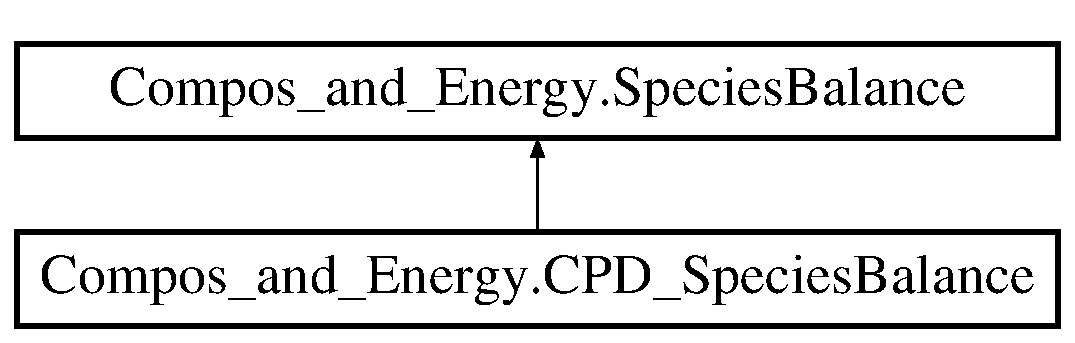
\includegraphics[height=2.000000cm]{classCompos__and__Energy_1_1CPD__SpeciesBalance}
\end{center}
\end{figure}
\subsection*{\-Public \-Member \-Functions}
\begin{DoxyCompactItemize}
\item 
\hypertarget{classCompos__and__Energy_1_1CPD__SpeciesBalance_a83897ac8fa055cd90b5a83751fe1b75f}{def {\bfseries \-\_\-\-\_\-init\-\_\-\-\_\-}}\label{classCompos__and__Energy_1_1CPD__SpeciesBalance_a83897ac8fa055cd90b5a83751fe1b75f}

\item 
def \hyperlink{classCompos__and__Energy_1_1SpeciesBalance_a5fec9a8d342543711abe2fc10632efb0}{\-Species\-Index}
\item 
def \hyperlink{classCompos__and__Energy_1_1SpeciesBalance_ae6b9b1a304a5b3686888725624c5e329}{moisture\-Volume\-Fraction}
\item 
def \hyperlink{classCompos__and__Energy_1_1SpeciesBalance_abeff1c726b62ba6c2d32173eb7f51d48}{\-Dulong}
\item 
def \hyperlink{classCompos__and__Energy_1_1SpeciesBalance_a05ae92b73a997e779c64bd2e6386a918}{correct\-U\-A}
\end{DoxyCompactItemize}
\subsection*{\-Public \-Attributes}
\begin{DoxyCompactItemize}
\item 
\hypertarget{classCompos__and__Energy_1_1CPD__SpeciesBalance_a05bc4dd081af063a2f798de068cf0b53}{{\bfseries \-Yields2\-Cols}}\label{classCompos__and__Energy_1_1CPD__SpeciesBalance_a05bc4dd081af063a2f798de068cf0b53}

\item 
\hypertarget{classCompos__and__Energy_1_1CPD__SpeciesBalance_a2af0b57b2b04248a7e1efdc25a8fbcd5}{{\bfseries \-Cols2\-Yields}}\label{classCompos__and__Energy_1_1CPD__SpeciesBalance_a2af0b57b2b04248a7e1efdc25a8fbcd5}

\item 
\hypertarget{classCompos__and__Energy_1_1CPD__SpeciesBalance_acea4a3c31b7c9a1faccd456e3b80ad79}{{\bfseries density\-Dry\-Coal}}\label{classCompos__and__Energy_1_1CPD__SpeciesBalance_acea4a3c31b7c9a1faccd456e3b80ad79}

\item 
\hypertarget{classCompos__and__Energy_1_1CPD__SpeciesBalance_ab4dd8c15931b59c83a8ba38fb68d05c7}{{\bfseries \-Yields}}\label{classCompos__and__Energy_1_1CPD__SpeciesBalance_ab4dd8c15931b59c83a8ba38fb68d05c7}

\item 
\hypertarget{classCompos__and__Energy_1_1CPD__SpeciesBalance_a1cd12c259989735108431296bab20c4b}{{\bfseries \-U\-A\-C}}\label{classCompos__and__Energy_1_1CPD__SpeciesBalance_a1cd12c259989735108431296bab20c4b}

\item 
\hypertarget{classCompos__and__Energy_1_1CPD__SpeciesBalance_a011a6a4062a54c304232d19ebdfd859a}{{\bfseries \-U\-A\-H}}\label{classCompos__and__Energy_1_1CPD__SpeciesBalance_a011a6a4062a54c304232d19ebdfd859a}

\item 
\hypertarget{classCompos__and__Energy_1_1CPD__SpeciesBalance_af91fbe0a0c1ef10bd6d0f76d6de0b61d}{{\bfseries \-U\-A\-N}}\label{classCompos__and__Energy_1_1CPD__SpeciesBalance_af91fbe0a0c1ef10bd6d0f76d6de0b61d}

\item 
\hypertarget{classCompos__and__Energy_1_1CPD__SpeciesBalance_aabd75abe8d7aaf92fd0b1a8c4070cbe5}{{\bfseries \-U\-A\-O}}\label{classCompos__and__Energy_1_1CPD__SpeciesBalance_aabd75abe8d7aaf92fd0b1a8c4070cbe5}

\item 
\hypertarget{classCompos__and__Energy_1_1CPD__SpeciesBalance_a26f545580381d73dd5e3de765f390467}{{\bfseries \-U\-A\-S}}\label{classCompos__and__Energy_1_1CPD__SpeciesBalance_a26f545580381d73dd5e3de765f390467}

\item 
\hypertarget{classCompos__and__Energy_1_1CPD__SpeciesBalance_abdcc4750f37c6b3ddae1b8c304d2ef39}{{\bfseries \-P\-A\-V\-M}}\label{classCompos__and__Energy_1_1CPD__SpeciesBalance_abdcc4750f37c6b3ddae1b8c304d2ef39}

\item 
\hypertarget{classCompos__and__Energy_1_1CPD__SpeciesBalance_a9bb2768aa3b30ee3d285857f590919aa}{{\bfseries \-P\-A\-F\-C}}\label{classCompos__and__Energy_1_1CPD__SpeciesBalance_a9bb2768aa3b30ee3d285857f590919aa}

\item 
\hypertarget{classCompos__and__Energy_1_1CPD__SpeciesBalance_a830a98945b252aa893371211068b9082}{{\bfseries gamma}}\label{classCompos__and__Energy_1_1CPD__SpeciesBalance_a830a98945b252aa893371211068b9082}

\item 
\hypertarget{classCompos__and__Energy_1_1CPD__SpeciesBalance_a5a950ab0a3201eeb3581ec2c52414571}{{\bfseries ny\-Tar}}\label{classCompos__and__Energy_1_1CPD__SpeciesBalance_a5a950ab0a3201eeb3581ec2c52414571}

\item 
\hypertarget{classCompos__and__Energy_1_1CPD__SpeciesBalance_a8b3dc599184ba5d0c4775940b954b98d}{{\bfseries ny\-Char}}\label{classCompos__and__Energy_1_1CPD__SpeciesBalance_a8b3dc599184ba5d0c4775940b954b98d}

\item 
\hypertarget{classCompos__and__Energy_1_1CPD__SpeciesBalance_af0d7f245d6ce8cf390523ba9b0047f82}{{\bfseries ny\-H2\-O}}\label{classCompos__and__Energy_1_1CPD__SpeciesBalance_af0d7f245d6ce8cf390523ba9b0047f82}

\item 
\hypertarget{classCompos__and__Energy_1_1CPD__SpeciesBalance_a434ba31c755f47c585b50bf52a1e5d80}{{\bfseries ny\-C\-O2}}\label{classCompos__and__Energy_1_1CPD__SpeciesBalance_a434ba31c755f47c585b50bf52a1e5d80}

\item 
\hypertarget{classCompos__and__Energy_1_1CPD__SpeciesBalance_afa6796afba2236182e5abc756e081798}{{\bfseries ny\-C\-H4}}\label{classCompos__and__Energy_1_1CPD__SpeciesBalance_afa6796afba2236182e5abc756e081798}

\item 
\hypertarget{classCompos__and__Energy_1_1CPD__SpeciesBalance_a04cfd2228bf5e1e99ec4504bff49cd15}{{\bfseries ny\-C\-O}}\label{classCompos__and__Energy_1_1CPD__SpeciesBalance_a04cfd2228bf5e1e99ec4504bff49cd15}

\item 
\hypertarget{classCompos__and__Energy_1_1CPD__SpeciesBalance_a65cb12ae9bb301703155e2d44d85296d}{{\bfseries ny\-N2}}\label{classCompos__and__Energy_1_1CPD__SpeciesBalance_a65cb12ae9bb301703155e2d44d85296d}

\end{DoxyCompactItemize}
\subsection*{\-Static \-Public \-Attributes}
\begin{DoxyCompactItemize}
\item 
\hypertarget{classCompos__and__Energy_1_1CPD__SpeciesBalance_ac3d3804ee4b37fd70a7955ca2060d180}{tuple {\bfseries \-H\-H\-V} = self.\-Dulong()}\label{classCompos__and__Energy_1_1CPD__SpeciesBalance_ac3d3804ee4b37fd70a7955ca2060d180}

\item 
\hypertarget{classCompos__and__Energy_1_1CPD__SpeciesBalance_a42f53843e09151397046910398f5d958}{tuple {\bfseries ashdry} = self.\-P\-Aash/(1-\/self.\-P\-Amoist)}\label{classCompos__and__Energy_1_1CPD__SpeciesBalance_a42f53843e09151397046910398f5d958}

\item 
\hypertarget{classCompos__and__Energy_1_1CPD__SpeciesBalance_a348aaf1b58522e52a78d044cbc96f7e7}{list {\bfseries char} = self.\-Yields\mbox{[}self.\-Species\-Index('\-Solid')\mbox{]}}\label{classCompos__and__Energy_1_1CPD__SpeciesBalance_a348aaf1b58522e52a78d044cbc96f7e7}

\item 
\hypertarget{classCompos__and__Energy_1_1CPD__SpeciesBalance_aca2fe35de233b1a0c7b3806e0becee53}{tuple {\bfseries vol} = (1-\/self.\-Yields\mbox{[}self.\-Species\-Index('\-Solid')\mbox{]})}\label{classCompos__and__Energy_1_1CPD__SpeciesBalance_aca2fe35de233b1a0c7b3806e0becee53}

\item 
\hypertarget{classCompos__and__Energy_1_1CPD__SpeciesBalance_a1fbb01c2d6b1f6ff41aa574fc48ebdd4}{int {\bfseries ash} = 100}\label{classCompos__and__Energy_1_1CPD__SpeciesBalance_a1fbb01c2d6b1f6ff41aa574fc48ebdd4}

\item 
\hypertarget{classCompos__and__Energy_1_1CPD__SpeciesBalance_aaf48fc4518fe773ed3fd06aa7636ecf6}{int {\bfseries sum} = 0}\label{classCompos__and__Energy_1_1CPD__SpeciesBalance_aaf48fc4518fe773ed3fd06aa7636ecf6}

\item 
\hypertarget{classCompos__and__Energy_1_1CPD__SpeciesBalance_a62a31b7e7146ef6fa335b9382ffaeb61}{float {\bfseries nu\-O2} = 0.\-5}\label{classCompos__and__Energy_1_1CPD__SpeciesBalance_a62a31b7e7146ef6fa335b9382ffaeb61}

\item 
\hypertarget{classCompos__and__Energy_1_1CPD__SpeciesBalance_a8e5bc50ca6f10a09164e2e1283cda937}{{\bfseries \-M\-Tar\-Check} = self.\-mu\-C\-Tar$\ast$\-M\-C+self.\-mu\-H\-Tar$\ast$\-M\-H+self.\-mu\-O\-Tar$\ast$\-M\-O+self.\-mu\-N\-Tar$\ast$\-M\-N+self.\-mu\-S\-Tar$\ast$\-M\-S}\label{classCompos__and__Energy_1_1CPD__SpeciesBalance_a8e5bc50ca6f10a09164e2e1283cda937}

\item 
\hypertarget{classCompos__and__Energy_1_1CPD__SpeciesBalance_af9f1b9cd71975f51962628577605391f}{tuple {\bfseries \-L\-H\-Var} = \-L\-H\-Vdaf$\ast$(self.\-P\-A\-F\-C+self.\-P\-A\-V\-M)}\label{classCompos__and__Energy_1_1CPD__SpeciesBalance_af9f1b9cd71975f51962628577605391f}

\item 
\hypertarget{classCompos__and__Energy_1_1CPD__SpeciesBalance_af840481e652bc3983f9098da223731a0}{{\bfseries mu\-C\-O2} = mu\-C\-Raw}\label{classCompos__and__Energy_1_1CPD__SpeciesBalance_af840481e652bc3983f9098da223731a0}

\item 
\hypertarget{classCompos__and__Energy_1_1CPD__SpeciesBalance_a9ba799336e7a9d65dd21da9d1e3689bc}{float {\bfseries mu\-H2\-O} = 0.\-5}\label{classCompos__and__Energy_1_1CPD__SpeciesBalance_a9ba799336e7a9d65dd21da9d1e3689bc}

\item 
\hypertarget{classCompos__and__Energy_1_1CPD__SpeciesBalance_a7338301550278542304fd2dc2b72c5fe}{float {\bfseries mu\-N2} = 0.\-5}\label{classCompos__and__Energy_1_1CPD__SpeciesBalance_a7338301550278542304fd2dc2b72c5fe}

\item 
\hypertarget{classCompos__and__Energy_1_1CPD__SpeciesBalance_a6bc192180926cbf92cd789bcf6f3176c}{{\bfseries mu\-S\-O2} = mu\-S\-Raw}\label{classCompos__and__Energy_1_1CPD__SpeciesBalance_a6bc192180926cbf92cd789bcf6f3176c}

\item 
\hypertarget{classCompos__and__Energy_1_1CPD__SpeciesBalance_a08b26e41f7d616dcca46b53fee7f240c}{float {\bfseries mu\-O2} = 0.\-5}\label{classCompos__and__Energy_1_1CPD__SpeciesBalance_a08b26e41f7d616dcca46b53fee7f240c}

\item 
\hypertarget{classCompos__and__Energy_1_1SpeciesBalance_a57d64961c8e035bf8087528adf669379}{{\bfseries sum\-U\-A} = self.\-U\-A\-C+self.\-U\-A\-H+self.\-U\-A\-O+self.\-U\-A\-N+self.\-U\-A\-S}\label{classCompos__and__Energy_1_1SpeciesBalance_a57d64961c8e035bf8087528adf669379}

\end{DoxyCompactItemize}


\subsection{\-Detailed \-Description}
\begin{DoxyVerb}This class calculates the Species and the Energy balance for CPD. See the manual for the formulas and more details.\end{DoxyVerb}
 

\subsection{\-Member \-Function \-Documentation}
\hypertarget{classCompos__and__Energy_1_1SpeciesBalance_a05ae92b73a997e779c64bd2e6386a918}{\index{\-Compos\-\_\-and\-\_\-\-Energy\-::\-C\-P\-D\-\_\-\-Species\-Balance@{\-Compos\-\_\-and\-\_\-\-Energy\-::\-C\-P\-D\-\_\-\-Species\-Balance}!correct\-U\-A@{correct\-U\-A}}
\index{correct\-U\-A@{correct\-U\-A}!Compos_and_Energy::CPD_SpeciesBalance@{\-Compos\-\_\-and\-\_\-\-Energy\-::\-C\-P\-D\-\_\-\-Species\-Balance}}
\subsubsection[{correct\-U\-A}]{\setlength{\rightskip}{0pt plus 5cm}def {\bf \-Compos\-\_\-and\-\_\-\-Energy.\-Species\-Balance.\-correct\-U\-A} (
\begin{DoxyParamCaption}
\item[{}]{self}
\end{DoxyParamCaption}
)\hspace{0.3cm}{\ttfamily  \mbox{[}inherited\mbox{]}}}}\label{classCompos__and__Energy_1_1SpeciesBalance_a05ae92b73a997e779c64bd2e6386a918}
\begin{DoxyVerb}Scale Ultimate Analysis to have sum=1\end{DoxyVerb}
 \hypertarget{classCompos__and__Energy_1_1SpeciesBalance_abeff1c726b62ba6c2d32173eb7f51d48}{\index{\-Compos\-\_\-and\-\_\-\-Energy\-::\-C\-P\-D\-\_\-\-Species\-Balance@{\-Compos\-\_\-and\-\_\-\-Energy\-::\-C\-P\-D\-\_\-\-Species\-Balance}!\-Dulong@{\-Dulong}}
\index{\-Dulong@{\-Dulong}!Compos_and_Energy::CPD_SpeciesBalance@{\-Compos\-\_\-and\-\_\-\-Energy\-::\-C\-P\-D\-\_\-\-Species\-Balance}}
\subsubsection[{\-Dulong}]{\setlength{\rightskip}{0pt plus 5cm}def {\bf \-Compos\-\_\-and\-\_\-\-Energy.\-Species\-Balance.\-Dulong} (
\begin{DoxyParamCaption}
\item[{}]{self}
\end{DoxyParamCaption}
)\hspace{0.3cm}{\ttfamily  \mbox{[}inherited\mbox{]}}}}\label{classCompos__and__Energy_1_1SpeciesBalance_abeff1c726b62ba6c2d32173eb7f51d48}
\begin{DoxyVerb}Uses the Dulong formular to calculate the Higher heating value. The output is in J/kg.\end{DoxyVerb}
 \hypertarget{classCompos__and__Energy_1_1SpeciesBalance_ae6b9b1a304a5b3686888725624c5e329}{\index{\-Compos\-\_\-and\-\_\-\-Energy\-::\-C\-P\-D\-\_\-\-Species\-Balance@{\-Compos\-\_\-and\-\_\-\-Energy\-::\-C\-P\-D\-\_\-\-Species\-Balance}!moisture\-Volume\-Fraction@{moisture\-Volume\-Fraction}}
\index{moisture\-Volume\-Fraction@{moisture\-Volume\-Fraction}!Compos_and_Energy::CPD_SpeciesBalance@{\-Compos\-\_\-and\-\_\-\-Energy\-::\-C\-P\-D\-\_\-\-Species\-Balance}}
\subsubsection[{moisture\-Volume\-Fraction}]{\setlength{\rightskip}{0pt plus 5cm}def {\bf \-Compos\-\_\-and\-\_\-\-Energy.\-Species\-Balance.\-moisture\-Volume\-Fraction} (
\begin{DoxyParamCaption}
\item[{}]{self}
\end{DoxyParamCaption}
)\hspace{0.3cm}{\ttfamily  \mbox{[}inherited\mbox{]}}}}\label{classCompos__and__Energy_1_1SpeciesBalance_ae6b9b1a304a5b3686888725624c5e329}
\begin{DoxyVerb}
calculate volume fraction of moisture
\end{DoxyVerb}
 \hypertarget{classCompos__and__Energy_1_1SpeciesBalance_a5fec9a8d342543711abe2fc10632efb0}{\index{\-Compos\-\_\-and\-\_\-\-Energy\-::\-C\-P\-D\-\_\-\-Species\-Balance@{\-Compos\-\_\-and\-\_\-\-Energy\-::\-C\-P\-D\-\_\-\-Species\-Balance}!\-Species\-Index@{\-Species\-Index}}
\index{\-Species\-Index@{\-Species\-Index}!Compos_and_Energy::CPD_SpeciesBalance@{\-Compos\-\_\-and\-\_\-\-Energy\-::\-C\-P\-D\-\_\-\-Species\-Balance}}
\subsubsection[{\-Species\-Index}]{\setlength{\rightskip}{0pt plus 5cm}def {\bf \-Compos\-\_\-and\-\_\-\-Energy.\-Species\-Balance.\-Species\-Index} (
\begin{DoxyParamCaption}
\item[{}]{self, }
\item[{}]{species}
\end{DoxyParamCaption}
)\hspace{0.3cm}{\ttfamily  \mbox{[}inherited\mbox{]}}}}\label{classCompos__and__Energy_1_1SpeciesBalance_a5fec9a8d342543711abe2fc10632efb0}
\begin{DoxyVerb}Returns the column number of the input species.\end{DoxyVerb}
 

\-The documentation for this class was generated from the following file\-:\begin{DoxyCompactItemize}
\item 
/home/map/git/pkp/src/\-Compos\-\_\-and\-\_\-\-Energy.\-py\end{DoxyCompactItemize}

\hypertarget{classModels_1_1DAEM}{\section{\-Models.\-D\-A\-E\-M \-Class \-Reference}
\label{classModels_1_1DAEM}\index{\-Models.\-D\-A\-E\-M@{\-Models.\-D\-A\-E\-M}}
}
\-Inheritance diagram for \-Models.\-D\-A\-E\-M\-:\begin{figure}[H]
\begin{center}
\leavevmode
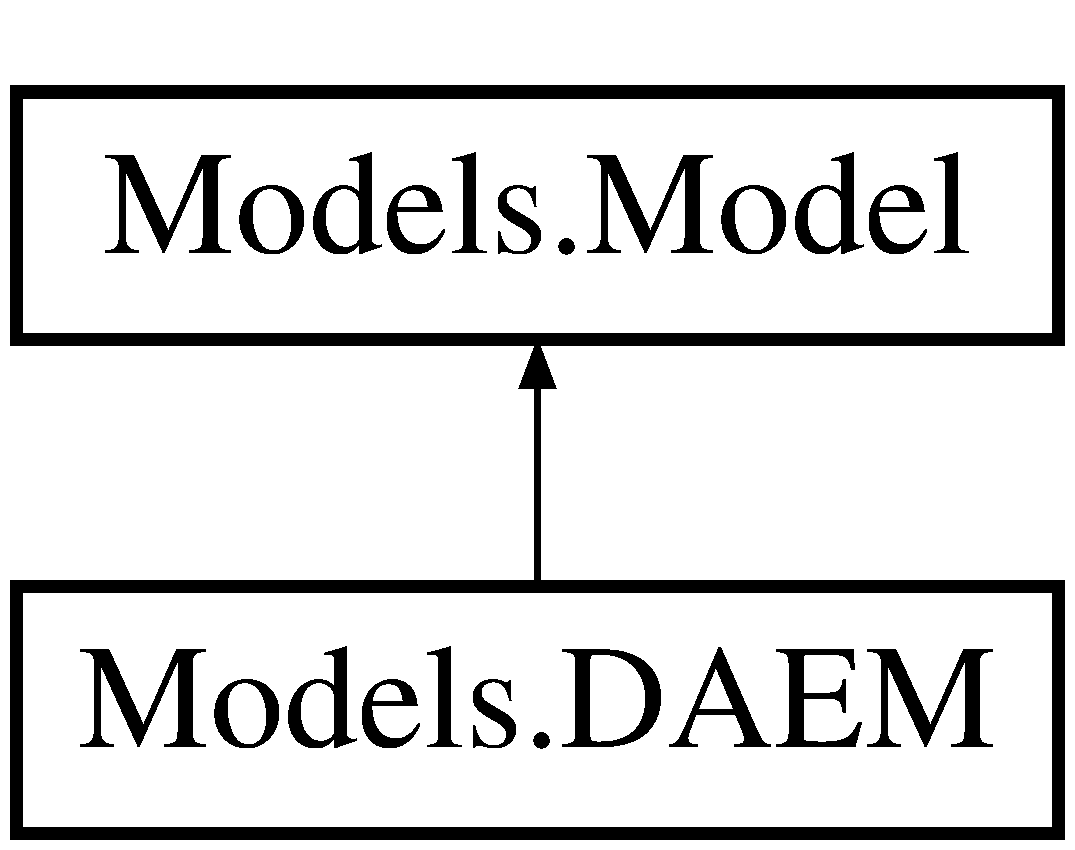
\includegraphics[height=2.000000cm]{classModels_1_1DAEM}
\end{center}
\end{figure}
\subsection*{\-Public \-Member \-Functions}
\begin{DoxyCompactItemize}
\item 
\hypertarget{classModels_1_1DAEM_aaa4b8bfa19485b2fd0684591d22540cb}{def {\bfseries \-\_\-\-\_\-init\-\_\-\-\_\-}}\label{classModels_1_1DAEM_aaa4b8bfa19485b2fd0684591d22540cb}

\item 
def \hyperlink{classModels_1_1DAEM_afd55a45fe616072ef780797eecc2e2e3}{set\-Nr\-Of\-Activation\-Energies}
\item 
def \hyperlink{classModels_1_1DAEM_ad3e09dbccde653e39af7dec35ea06f9b}{\-Nr\-Of\-Activation\-Energies}
\item 
def \hyperlink{classModels_1_1DAEM_ac861fdf6e0863a4e20f88021cb0e85c9}{calc\-Mass}
\item 
def \hyperlink{classModels_1_1Model_a317ed848b969dbe3a96dd05e8b771900}{plt\-Yield}
\item 
def \hyperlink{classModels_1_1Model_aa35c741babf8f141df48c4021e0664e4}{plt\-Rate}
\item 
def \hyperlink{classModels_1_1Model_a3396d6ca1a7b7d66e55ada8c3c7a509e}{max\-Length\-Of\-Vectors}
\item 
def \hyperlink{classModels_1_1Model_ae404a691e48bfe4eafcdfdd09f1dae48}{plot}
\item 
def \hyperlink{classModels_1_1Model_a010945ed2adff59a7a5fce36025e7a97}{derive\-C}
\item 
def \hyperlink{classModels_1_1Model_a7c9280e33f9e0d46703cebc131008c65}{calc\-Rate}
\item 
def \hyperlink{classModels_1_1Model_a818f207e2a4bd0e9a3720ca611960e5a}{set\-Param\-Vector}
\item 
def \hyperlink{classModels_1_1Model_a13c76a0fe24d43cdc4d21fbc73fa96fa}{\-Param\-Vector}
\item 
def \hyperlink{classModels_1_1Model_ad3e627980d9e781bf7b2c9ff900ca06b}{\-Error\-Yield}
\item 
def \hyperlink{classModels_1_1Model_a3050eb39341f318d8d88b172f88bd240}{\-Error\-Rate}
\item 
def \hyperlink{classModels_1_1Model_adcb987bccae63a742490ea1e6d5f7a74}{mk\-Simple\-Result\-Files}
\item 
def \hyperlink{classModels_1_1Model_ac28252ae5cd6b5ecd4c5d006a0e6567d}{set\-Dt4\-Intergrate}
\end{DoxyCompactItemize}
\subsection*{\-Public \-Attributes}
\begin{DoxyCompactItemize}
\item 
\hypertarget{classModels_1_1DAEM_aec08a04e258d654483d9a5dc8d999ab9}{{\bfseries \-O\-D\-E\-\_\-hmax}}\label{classModels_1_1DAEM_aec08a04e258d654483d9a5dc8d999ab9}

\item 
\hypertarget{classModels_1_1DAEM_a4a4677dd5d017d4ef8803d98a067f0ba}{{\bfseries \-Nr\-Of\-Activation\-Energies}}\label{classModels_1_1DAEM_a4a4677dd5d017d4ef8803d98a067f0ba}

\item 
\hypertarget{classModels_1_1DAEM_a63861d8311d112cfd894639960c589da}{{\bfseries const\-Dt}}\label{classModels_1_1DAEM_a63861d8311d112cfd894639960c589da}

\item 
\hypertarget{classModels_1_1DAEM_af93597d730ec6e6a12828598f42f06bc}{{\bfseries \-E\-\_\-\-List}}\label{classModels_1_1DAEM_af93597d730ec6e6a12828598f42f06bc}

\item 
\hypertarget{classModels_1_1Model_a3f71983de5f8b86bec47929213b900ec}{{\bfseries const\-Dt\-Vec}}\label{classModels_1_1Model_a3f71983de5f8b86bec47929213b900ec}

\end{DoxyCompactItemize}


\subsection{\-Detailed \-Description}
\begin{DoxyVerb}Calculates the devolatilization reaction using the Distributed Activation Energy Model.\end{DoxyVerb}
 

\subsection{\-Member \-Function \-Documentation}
\hypertarget{classModels_1_1DAEM_ac861fdf6e0863a4e20f88021cb0e85c9}{\index{\-Models\-::\-D\-A\-E\-M@{\-Models\-::\-D\-A\-E\-M}!calc\-Mass@{calc\-Mass}}
\index{calc\-Mass@{calc\-Mass}!Models::DAEM@{\-Models\-::\-D\-A\-E\-M}}
\subsubsection[{calc\-Mass}]{\setlength{\rightskip}{0pt plus 5cm}def {\bf \-Models.\-D\-A\-E\-M.\-calc\-Mass} (
\begin{DoxyParamCaption}
\item[{}]{self, }
\item[{}]{fgdvc, }
\item[{}]{time, }
\item[{}]{\-T, }
\item[{}]{\-Name}
\end{DoxyParamCaption}
)}}\label{classModels_1_1DAEM_ac861fdf6e0863a4e20f88021cb0e85c9}
\begin{DoxyVerb}Outputs the mass(t) using the model specific equation.\end{DoxyVerb}
 \hypertarget{classModels_1_1Model_a7c9280e33f9e0d46703cebc131008c65}{\index{\-Models\-::\-D\-A\-E\-M@{\-Models\-::\-D\-A\-E\-M}!calc\-Rate@{calc\-Rate}}
\index{calc\-Rate@{calc\-Rate}!Models::DAEM@{\-Models\-::\-D\-A\-E\-M}}
\subsubsection[{calc\-Rate}]{\setlength{\rightskip}{0pt plus 5cm}def {\bf \-Models.\-Model.\-calc\-Rate} (
\begin{DoxyParamCaption}
\item[{}]{self, }
\item[{}]{fgdvc, }
\item[{}]{time, }
\item[{}]{\-T, }
\item[{}]{\-Name}
\end{DoxyParamCaption}
)\hspace{0.3cm}{\ttfamily  \mbox{[}inherited\mbox{]}}}}\label{classModels_1_1Model_a7c9280e33f9e0d46703cebc131008c65}
\begin{DoxyVerb}Generates the Rates using the yields vector and a CDS.\end{DoxyVerb}
 \hypertarget{classModels_1_1Model_a010945ed2adff59a7a5fce36025e7a97}{\index{\-Models\-::\-D\-A\-E\-M@{\-Models\-::\-D\-A\-E\-M}!derive\-C@{derive\-C}}
\index{derive\-C@{derive\-C}!Models::DAEM@{\-Models\-::\-D\-A\-E\-M}}
\subsubsection[{derive\-C}]{\setlength{\rightskip}{0pt plus 5cm}def {\bf \-Models.\-Model.\-derive\-C} (
\begin{DoxyParamCaption}
\item[{}]{self, }
\item[{}]{fgdvc, }
\item[{}]{y\-Vector}
\end{DoxyParamCaption}
)\hspace{0.3cm}{\ttfamily  \mbox{[}inherited\mbox{]}}}}\label{classModels_1_1Model_a010945ed2adff59a7a5fce36025e7a97}
\begin{DoxyVerb}Returns a CDS of the inputted yVector.\end{DoxyVerb}
 \hypertarget{classModels_1_1Model_a3050eb39341f318d8d88b172f88bd240}{\index{\-Models\-::\-D\-A\-E\-M@{\-Models\-::\-D\-A\-E\-M}!\-Error\-Rate@{\-Error\-Rate}}
\index{\-Error\-Rate@{\-Error\-Rate}!Models::DAEM@{\-Models\-::\-D\-A\-E\-M}}
\subsubsection[{\-Error\-Rate}]{\setlength{\rightskip}{0pt plus 5cm}def {\bf \-Models.\-Model.\-Error\-Rate} (
\begin{DoxyParamCaption}
\item[{}]{self, }
\item[{}]{fgdvc, }
\item[{}]{\-Species}
\end{DoxyParamCaption}
)\hspace{0.3cm}{\ttfamily  \mbox{[}inherited\mbox{]}}}}\label{classModels_1_1Model_a3050eb39341f318d8d88b172f88bd240}
\begin{DoxyVerb}Returns the absolute deviation per point between the fitted and the original rate curve.\end{DoxyVerb}
 \hypertarget{classModels_1_1Model_ad3e627980d9e781bf7b2c9ff900ca06b}{\index{\-Models\-::\-D\-A\-E\-M@{\-Models\-::\-D\-A\-E\-M}!\-Error\-Yield@{\-Error\-Yield}}
\index{\-Error\-Yield@{\-Error\-Yield}!Models::DAEM@{\-Models\-::\-D\-A\-E\-M}}
\subsubsection[{\-Error\-Yield}]{\setlength{\rightskip}{0pt plus 5cm}def {\bf \-Models.\-Model.\-Error\-Yield} (
\begin{DoxyParamCaption}
\item[{}]{self, }
\item[{}]{fgdvc, }
\item[{}]{\-Species}
\end{DoxyParamCaption}
)\hspace{0.3cm}{\ttfamily  \mbox{[}inherited\mbox{]}}}}\label{classModels_1_1Model_ad3e627980d9e781bf7b2c9ff900ca06b}
\begin{DoxyVerb}Returns the absolute deviation per point between the fitted and the original yield curve.\end{DoxyVerb}
 \hypertarget{classModels_1_1Model_a3396d6ca1a7b7d66e55ada8c3c7a509e}{\index{\-Models\-::\-D\-A\-E\-M@{\-Models\-::\-D\-A\-E\-M}!max\-Length\-Of\-Vectors@{max\-Length\-Of\-Vectors}}
\index{max\-Length\-Of\-Vectors@{max\-Length\-Of\-Vectors}!Models::DAEM@{\-Models\-::\-D\-A\-E\-M}}
\subsubsection[{max\-Length\-Of\-Vectors}]{\setlength{\rightskip}{0pt plus 5cm}def {\bf \-Models.\-Model.\-max\-Length\-Of\-Vectors} (
\begin{DoxyParamCaption}
\item[{}]{self, }
\item[{}]{fgdvc\-\_\-list}
\end{DoxyParamCaption}
)\hspace{0.3cm}{\ttfamily  \mbox{[}inherited\mbox{]}}}}\label{classModels_1_1Model_a3396d6ca1a7b7d66e55ada8c3c7a509e}
\begin{DoxyVerb}Returns the minimum lenght of a all vectors from the several runs.\end{DoxyVerb}
 \hypertarget{classModels_1_1Model_adcb987bccae63a742490ea1e6d5f7a74}{\index{\-Models\-::\-D\-A\-E\-M@{\-Models\-::\-D\-A\-E\-M}!mk\-Simple\-Result\-Files@{mk\-Simple\-Result\-Files}}
\index{mk\-Simple\-Result\-Files@{mk\-Simple\-Result\-Files}!Models::DAEM@{\-Models\-::\-D\-A\-E\-M}}
\subsubsection[{mk\-Simple\-Result\-Files}]{\setlength{\rightskip}{0pt plus 5cm}def {\bf \-Models.\-Model.\-mk\-Simple\-Result\-Files} (
\begin{DoxyParamCaption}
\item[{}]{self, }
\item[{}]{fgdvc\-\_\-list, }
\item[{}]{\-Species}
\end{DoxyParamCaption}
)\hspace{0.3cm}{\ttfamily  \mbox{[}inherited\mbox{]}}}}\label{classModels_1_1Model_adcb987bccae63a742490ea1e6d5f7a74}
\begin{DoxyVerb}Simple result file if no fitting is carried out. Writes only the transformed results into a file.\end{DoxyVerb}
 \hypertarget{classModels_1_1DAEM_ad3e09dbccde653e39af7dec35ea06f9b}{\index{\-Models\-::\-D\-A\-E\-M@{\-Models\-::\-D\-A\-E\-M}!\-Nr\-Of\-Activation\-Energies@{\-Nr\-Of\-Activation\-Energies}}
\index{\-Nr\-Of\-Activation\-Energies@{\-Nr\-Of\-Activation\-Energies}!Models::DAEM@{\-Models\-::\-D\-A\-E\-M}}
\subsubsection[{\-Nr\-Of\-Activation\-Energies}]{\setlength{\rightskip}{0pt plus 5cm}def \-Models.\-D\-A\-E\-M.\-Nr\-Of\-Activation\-Energies (
\begin{DoxyParamCaption}
\item[{}]{self}
\end{DoxyParamCaption}
)}}\label{classModels_1_1DAEM_ad3e09dbccde653e39af7dec35ea06f9b}
\begin{DoxyVerb}Returns the number of activation enrgies the integral shall be solved for (using Simpson Rule).\end{DoxyVerb}
 \hypertarget{classModels_1_1Model_a13c76a0fe24d43cdc4d21fbc73fa96fa}{\index{\-Models\-::\-D\-A\-E\-M@{\-Models\-::\-D\-A\-E\-M}!\-Param\-Vector@{\-Param\-Vector}}
\index{\-Param\-Vector@{\-Param\-Vector}!Models::DAEM@{\-Models\-::\-D\-A\-E\-M}}
\subsubsection[{\-Param\-Vector}]{\setlength{\rightskip}{0pt plus 5cm}def {\bf \-Models.\-Model.\-Param\-Vector} (
\begin{DoxyParamCaption}
\item[{}]{self}
\end{DoxyParamCaption}
)\hspace{0.3cm}{\ttfamily  \mbox{[}inherited\mbox{]}}}}\label{classModels_1_1Model_a13c76a0fe24d43cdc4d21fbc73fa96fa}
\begin{DoxyVerb}Returns the Vector containing the kinetic parameter of the Model (refering to the child model).\end{DoxyVerb}
 \hypertarget{classModels_1_1Model_ae404a691e48bfe4eafcdfdd09f1dae48}{\index{\-Models\-::\-D\-A\-E\-M@{\-Models\-::\-D\-A\-E\-M}!plot@{plot}}
\index{plot@{plot}!Models::DAEM@{\-Models\-::\-D\-A\-E\-M}}
\subsubsection[{plot}]{\setlength{\rightskip}{0pt plus 5cm}def {\bf \-Models.\-Model.\-plot} (
\begin{DoxyParamCaption}
\item[{}]{self, }
\item[{}]{fgdvc\-\_\-list, }
\item[{}]{\-Species}
\end{DoxyParamCaption}
)\hspace{0.3cm}{\ttfamily  \mbox{[}inherited\mbox{]}}}}\label{classModels_1_1Model_ae404a691e48bfe4eafcdfdd09f1dae48}
\begin{DoxyVerb}Plot the yield and the rates over time with two curves: one is the original data, the other the fitting curve. Also file 'PyrolysisProgramName-Species.out' (e.g. 'CPD-CO2.out') containing the time (s), yields (kg/kg), rates (kg/(kg s)).\end{DoxyVerb}
 \hypertarget{classModels_1_1Model_aa35c741babf8f141df48c4021e0664e4}{\index{\-Models\-::\-D\-A\-E\-M@{\-Models\-::\-D\-A\-E\-M}!plt\-Rate@{plt\-Rate}}
\index{plt\-Rate@{plt\-Rate}!Models::DAEM@{\-Models\-::\-D\-A\-E\-M}}
\subsubsection[{plt\-Rate}]{\setlength{\rightskip}{0pt plus 5cm}def {\bf \-Models.\-Model.\-plt\-Rate} (
\begin{DoxyParamCaption}
\item[{}]{self, }
\item[{}]{fgdvc\-\_\-list, }
\item[{}]{x\-Value\-To\-Plot, }
\item[{}]{y\-Value\-To\-Plot}
\end{DoxyParamCaption}
)\hspace{0.3cm}{\ttfamily  \mbox{[}inherited\mbox{]}}}}\label{classModels_1_1Model_aa35c741babf8f141df48c4021e0664e4}
\begin{DoxyVerb}Plots the rates (to select with yValueToPlot) over Time or Temperature (to slect with xValueToPlot).\end{DoxyVerb}
 \hypertarget{classModels_1_1Model_a317ed848b969dbe3a96dd05e8b771900}{\index{\-Models\-::\-D\-A\-E\-M@{\-Models\-::\-D\-A\-E\-M}!plt\-Yield@{plt\-Yield}}
\index{plt\-Yield@{plt\-Yield}!Models::DAEM@{\-Models\-::\-D\-A\-E\-M}}
\subsubsection[{plt\-Yield}]{\setlength{\rightskip}{0pt plus 5cm}def {\bf \-Models.\-Model.\-plt\-Yield} (
\begin{DoxyParamCaption}
\item[{}]{self, }
\item[{}]{fgdvc\-\_\-list, }
\item[{}]{x\-Value\-To\-Plot, }
\item[{}]{y\-Value\-To\-Plot}
\end{DoxyParamCaption}
)\hspace{0.3cm}{\ttfamily  \mbox{[}inherited\mbox{]}}}}\label{classModels_1_1Model_a317ed848b969dbe3a96dd05e8b771900}
\begin{DoxyVerb}Plots the yields (to select with yValueToPlot) over Time or Temperature (to slect with xValueToPlot).\end{DoxyVerb}
 \hypertarget{classModels_1_1Model_ac28252ae5cd6b5ecd4c5d006a0e6567d}{\index{\-Models\-::\-D\-A\-E\-M@{\-Models\-::\-D\-A\-E\-M}!set\-Dt4\-Intergrate@{set\-Dt4\-Intergrate}}
\index{set\-Dt4\-Intergrate@{set\-Dt4\-Intergrate}!Models::DAEM@{\-Models\-::\-D\-A\-E\-M}}
\subsubsection[{set\-Dt4\-Intergrate}]{\setlength{\rightskip}{0pt plus 5cm}def {\bf \-Models.\-Model.\-set\-Dt4\-Intergrate} (
\begin{DoxyParamCaption}
\item[{}]{self, }
\item[{}]{constant\-Dt}
\end{DoxyParamCaption}
)\hspace{0.3cm}{\ttfamily  \mbox{[}inherited\mbox{]}}}}\label{classModels_1_1Model_ac28252ae5cd6b5ecd4c5d006a0e6567d}
\begin{DoxyVerb}constantDt allows the option to define numerical time step to solve the ODE. The outputted results ever equal the imported time list (when applying method calcMass Time = [t0,t1,t2,t3,t4]. If these time steps are too large, then is this defined dt used to solve the ODE and the results are linear interploated that way that they correspond to the imported time vector. To reset it, just set constantDt to False.\end{DoxyVerb}
 \hypertarget{classModels_1_1DAEM_afd55a45fe616072ef780797eecc2e2e3}{\index{\-Models\-::\-D\-A\-E\-M@{\-Models\-::\-D\-A\-E\-M}!set\-Nr\-Of\-Activation\-Energies@{set\-Nr\-Of\-Activation\-Energies}}
\index{set\-Nr\-Of\-Activation\-Energies@{set\-Nr\-Of\-Activation\-Energies}!Models::DAEM@{\-Models\-::\-D\-A\-E\-M}}
\subsubsection[{set\-Nr\-Of\-Activation\-Energies}]{\setlength{\rightskip}{0pt plus 5cm}def {\bf \-Models.\-D\-A\-E\-M.\-set\-Nr\-Of\-Activation\-Energies} (
\begin{DoxyParamCaption}
\item[{}]{self, }
\item[{}]{\-Nr\-Of\-E}
\end{DoxyParamCaption}
)}}\label{classModels_1_1DAEM_afd55a45fe616072ef780797eecc2e2e3}
\begin{DoxyVerb}Define for how many activation energies of the range of the whole distribution the integral shall be solved (using Simpson Rule).\end{DoxyVerb}
 \hypertarget{classModels_1_1Model_a818f207e2a4bd0e9a3720ca611960e5a}{\index{\-Models\-::\-D\-A\-E\-M@{\-Models\-::\-D\-A\-E\-M}!set\-Param\-Vector@{set\-Param\-Vector}}
\index{set\-Param\-Vector@{set\-Param\-Vector}!Models::DAEM@{\-Models\-::\-D\-A\-E\-M}}
\subsubsection[{set\-Param\-Vector}]{\setlength{\rightskip}{0pt plus 5cm}def {\bf \-Models.\-Model.\-set\-Param\-Vector} (
\begin{DoxyParamCaption}
\item[{}]{self, }
\item[{}]{\-Parameter\-List}
\end{DoxyParamCaption}
)\hspace{0.3cm}{\ttfamily  \mbox{[}inherited\mbox{]}}}}\label{classModels_1_1Model_a818f207e2a4bd0e9a3720ca611960e5a}
\begin{DoxyVerb}Sets the Vector containing the kinetic parameter of the Model (refering to the child model).\end{DoxyVerb}
 

\-The documentation for this class was generated from the following file\-:\begin{DoxyCompactItemize}
\item 
/home/map/git/pkp/src/\-Models.\-py\end{DoxyCompactItemize}

\hypertarget{classFGDVC__Result_1_1FGDVC__Result}{\section{\-F\-G\-D\-V\-C\-\_\-\-Result.\-F\-G\-D\-V\-C\-\_\-\-Result \-Class \-Reference}
\label{classFGDVC__Result_1_1FGDVC__Result}\index{\-F\-G\-D\-V\-C\-\_\-\-Result.\-F\-G\-D\-V\-C\-\_\-\-Result@{\-F\-G\-D\-V\-C\-\_\-\-Result.\-F\-G\-D\-V\-C\-\_\-\-Result}}
}
\subsection*{\-Public \-Member \-Functions}
\begin{DoxyCompactItemize}
\item 
\hypertarget{classFGDVC__Result_1_1FGDVC__Result_a2214547494b8e49e33681f05d5560939}{def {\bfseries \-\_\-\-\_\-init\-\_\-\-\_\-}}\label{classFGDVC__Result_1_1FGDVC__Result_a2214547494b8e49e33681f05d5560939}

\item 
def \hyperlink{classFGDVC__Result_1_1FGDVC__Result_a96334603fc6df5e0e13b0c63d69936eb}{\-Yields\-\_\-all}
\item 
def \hyperlink{classFGDVC__Result_1_1FGDVC__Result_a89d6e2a6ece5e2beb03187011fb5f4bb}{\-Rates\-\_\-all}
\item 
def \hyperlink{classFGDVC__Result_1_1FGDVC__Result_a81a8ca345a6d024a3c33568dbbcb119e}{\-Dict\-Yields2\-Cols}
\item 
def \hyperlink{classFGDVC__Result_1_1FGDVC__Result_a415f223456d256d52afea60b74916676}{\-Dict\-Cols2\-Yields}
\item 
def \hyperlink{classFGDVC__Result_1_1FGDVC__Result_ad3c91913db48efad9c33a0f2d87b9bfb}{\-Final\-Yields}
\item 
def \hyperlink{classFGDVC__Result_1_1FGDVC__Result_a778588f293b3b544482f26ab63fe3d57}{\-File\-Path}
\item 
def \hyperlink{classFGDVC__Result_1_1FGDVC__Result_ad85ce8419074dca37993ce9a4665dddd}{\-Name}
\end{DoxyCompactItemize}
\subsection*{\-Public \-Attributes}
\begin{DoxyCompactItemize}
\item 
\hypertarget{classFGDVC__Result_1_1FGDVC__Result_aa52ef0bb67b48d181097912e5fe1741f}{{\bfseries \-Yields2\-Cols}}\label{classFGDVC__Result_1_1FGDVC__Result_aa52ef0bb67b48d181097912e5fe1741f}

\item 
\hypertarget{classFGDVC__Result_1_1FGDVC__Result_ab73aa267199cb6ea215b27776066daba}{{\bfseries \-Cols2\-Yields}}\label{classFGDVC__Result_1_1FGDVC__Result_ab73aa267199cb6ea215b27776066daba}

\end{DoxyCompactItemize}


\subsection{\-Detailed \-Description}
\begin{DoxyVerb}Reads the FG-DVC input and saves the values in one array. The results include the yields (from 'gasyields.txt') and the rates. The rates for all species except the solids (here a CDS is used) are imported from 'gasrates.txt'. The H_2 yields were calculated by subtract all other species except parafins and olefins from the total yields (see FG-DVC manual). This H_2-yield curve was smoothed and derived using a CDS to generate the H_2 rates. The parafins and olefins are added into the tar. This class also contains the dictionaries for the columns in the array - the name of the species. These dictionaries are FG-DVC-Version dependent and the only thing which has to be changed for the case of a new release of FG-DVC with a new order of species in the result files (this was made for Versions 8.2.2. and 8.2.3.).\end{DoxyVerb}
 

\subsection{\-Member \-Function \-Documentation}
\hypertarget{classFGDVC__Result_1_1FGDVC__Result_a415f223456d256d52afea60b74916676}{\index{\-F\-G\-D\-V\-C\-\_\-\-Result\-::\-F\-G\-D\-V\-C\-\_\-\-Result@{\-F\-G\-D\-V\-C\-\_\-\-Result\-::\-F\-G\-D\-V\-C\-\_\-\-Result}!\-Dict\-Cols2\-Yields@{\-Dict\-Cols2\-Yields}}
\index{\-Dict\-Cols2\-Yields@{\-Dict\-Cols2\-Yields}!FGDVC_Result::FGDVC_Result@{\-F\-G\-D\-V\-C\-\_\-\-Result\-::\-F\-G\-D\-V\-C\-\_\-\-Result}}
\subsubsection[{\-Dict\-Cols2\-Yields}]{\setlength{\rightskip}{0pt plus 5cm}def {\bf \-F\-G\-D\-V\-C\-\_\-\-Result.\-F\-G\-D\-V\-C\-\_\-\-Result.\-Dict\-Cols2\-Yields} (
\begin{DoxyParamCaption}
\item[{}]{self}
\end{DoxyParamCaption}
)}}\label{classFGDVC__Result_1_1FGDVC__Result_a415f223456d256d52afea60b74916676}
\begin{DoxyVerb}Returns the whole Dictionary Columns of the matrix to Yield names\end{DoxyVerb}
 \hypertarget{classFGDVC__Result_1_1FGDVC__Result_a81a8ca345a6d024a3c33568dbbcb119e}{\index{\-F\-G\-D\-V\-C\-\_\-\-Result\-::\-F\-G\-D\-V\-C\-\_\-\-Result@{\-F\-G\-D\-V\-C\-\_\-\-Result\-::\-F\-G\-D\-V\-C\-\_\-\-Result}!\-Dict\-Yields2\-Cols@{\-Dict\-Yields2\-Cols}}
\index{\-Dict\-Yields2\-Cols@{\-Dict\-Yields2\-Cols}!FGDVC_Result::FGDVC_Result@{\-F\-G\-D\-V\-C\-\_\-\-Result\-::\-F\-G\-D\-V\-C\-\_\-\-Result}}
\subsubsection[{\-Dict\-Yields2\-Cols}]{\setlength{\rightskip}{0pt plus 5cm}def {\bf \-F\-G\-D\-V\-C\-\_\-\-Result.\-F\-G\-D\-V\-C\-\_\-\-Result.\-Dict\-Yields2\-Cols} (
\begin{DoxyParamCaption}
\item[{}]{self}
\end{DoxyParamCaption}
)}}\label{classFGDVC__Result_1_1FGDVC__Result_a81a8ca345a6d024a3c33568dbbcb119e}
\begin{DoxyVerb}Returns the whole Dictionary Yield names to Columns of the matrix\end{DoxyVerb}
 \hypertarget{classFGDVC__Result_1_1FGDVC__Result_a778588f293b3b544482f26ab63fe3d57}{\index{\-F\-G\-D\-V\-C\-\_\-\-Result\-::\-F\-G\-D\-V\-C\-\_\-\-Result@{\-F\-G\-D\-V\-C\-\_\-\-Result\-::\-F\-G\-D\-V\-C\-\_\-\-Result}!\-File\-Path@{\-File\-Path}}
\index{\-File\-Path@{\-File\-Path}!FGDVC_Result::FGDVC_Result@{\-F\-G\-D\-V\-C\-\_\-\-Result\-::\-F\-G\-D\-V\-C\-\_\-\-Result}}
\subsubsection[{\-File\-Path}]{\setlength{\rightskip}{0pt plus 5cm}def {\bf \-F\-G\-D\-V\-C\-\_\-\-Result.\-F\-G\-D\-V\-C\-\_\-\-Result.\-File\-Path} (
\begin{DoxyParamCaption}
\item[{}]{self}
\end{DoxyParamCaption}
)}}\label{classFGDVC__Result_1_1FGDVC__Result_a778588f293b3b544482f26ab63fe3d57}
\begin{DoxyVerb}Returns the FG-DVC File path\end{DoxyVerb}
 \hypertarget{classFGDVC__Result_1_1FGDVC__Result_ad3c91913db48efad9c33a0f2d87b9bfb}{\index{\-F\-G\-D\-V\-C\-\_\-\-Result\-::\-F\-G\-D\-V\-C\-\_\-\-Result@{\-F\-G\-D\-V\-C\-\_\-\-Result\-::\-F\-G\-D\-V\-C\-\_\-\-Result}!\-Final\-Yields@{\-Final\-Yields}}
\index{\-Final\-Yields@{\-Final\-Yields}!FGDVC_Result::FGDVC_Result@{\-F\-G\-D\-V\-C\-\_\-\-Result\-::\-F\-G\-D\-V\-C\-\_\-\-Result}}
\subsubsection[{\-Final\-Yields}]{\setlength{\rightskip}{0pt plus 5cm}def {\bf \-F\-G\-D\-V\-C\-\_\-\-Result.\-F\-G\-D\-V\-C\-\_\-\-Result.\-Final\-Yields} (
\begin{DoxyParamCaption}
\item[{}]{self}
\end{DoxyParamCaption}
)}}\label{classFGDVC__Result_1_1FGDVC__Result_ad3c91913db48efad9c33a0f2d87b9bfb}
\begin{DoxyVerb}Returns the last line of the Array, containing the yields at the time=time_End\end{DoxyVerb}
 \hypertarget{classFGDVC__Result_1_1FGDVC__Result_ad85ce8419074dca37993ce9a4665dddd}{\index{\-F\-G\-D\-V\-C\-\_\-\-Result\-::\-F\-G\-D\-V\-C\-\_\-\-Result@{\-F\-G\-D\-V\-C\-\_\-\-Result\-::\-F\-G\-D\-V\-C\-\_\-\-Result}!\-Name@{\-Name}}
\index{\-Name@{\-Name}!FGDVC_Result::FGDVC_Result@{\-F\-G\-D\-V\-C\-\_\-\-Result\-::\-F\-G\-D\-V\-C\-\_\-\-Result}}
\subsubsection[{\-Name}]{\setlength{\rightskip}{0pt plus 5cm}def {\bf \-F\-G\-D\-V\-C\-\_\-\-Result.\-F\-G\-D\-V\-C\-\_\-\-Result.\-Name} (
\begin{DoxyParamCaption}
\item[{}]{self}
\end{DoxyParamCaption}
)}}\label{classFGDVC__Result_1_1FGDVC__Result_ad85ce8419074dca37993ce9a4665dddd}
\begin{DoxyVerb}returns 'FG-DVC' as the name of the Program\end{DoxyVerb}
 \hypertarget{classFGDVC__Result_1_1FGDVC__Result_a89d6e2a6ece5e2beb03187011fb5f4bb}{\index{\-F\-G\-D\-V\-C\-\_\-\-Result\-::\-F\-G\-D\-V\-C\-\_\-\-Result@{\-F\-G\-D\-V\-C\-\_\-\-Result\-::\-F\-G\-D\-V\-C\-\_\-\-Result}!\-Rates\-\_\-all@{\-Rates\-\_\-all}}
\index{\-Rates\-\_\-all@{\-Rates\-\_\-all}!FGDVC_Result::FGDVC_Result@{\-F\-G\-D\-V\-C\-\_\-\-Result\-::\-F\-G\-D\-V\-C\-\_\-\-Result}}
\subsubsection[{\-Rates\-\_\-all}]{\setlength{\rightskip}{0pt plus 5cm}def {\bf \-F\-G\-D\-V\-C\-\_\-\-Result.\-F\-G\-D\-V\-C\-\_\-\-Result.\-Rates\-\_\-all} (
\begin{DoxyParamCaption}
\item[{}]{self}
\end{DoxyParamCaption}
)}}\label{classFGDVC__Result_1_1FGDVC__Result_a89d6e2a6ece5e2beb03187011fb5f4bb}
\begin{DoxyVerb}Returns the whole result matrix of the Rates.\end{DoxyVerb}
 \hypertarget{classFGDVC__Result_1_1FGDVC__Result_a96334603fc6df5e0e13b0c63d69936eb}{\index{\-F\-G\-D\-V\-C\-\_\-\-Result\-::\-F\-G\-D\-V\-C\-\_\-\-Result@{\-F\-G\-D\-V\-C\-\_\-\-Result\-::\-F\-G\-D\-V\-C\-\_\-\-Result}!\-Yields\-\_\-all@{\-Yields\-\_\-all}}
\index{\-Yields\-\_\-all@{\-Yields\-\_\-all}!FGDVC_Result::FGDVC_Result@{\-F\-G\-D\-V\-C\-\_\-\-Result\-::\-F\-G\-D\-V\-C\-\_\-\-Result}}
\subsubsection[{\-Yields\-\_\-all}]{\setlength{\rightskip}{0pt plus 5cm}def {\bf \-F\-G\-D\-V\-C\-\_\-\-Result.\-F\-G\-D\-V\-C\-\_\-\-Result.\-Yields\-\_\-all} (
\begin{DoxyParamCaption}
\item[{}]{self}
\end{DoxyParamCaption}
)}}\label{classFGDVC__Result_1_1FGDVC__Result_a96334603fc6df5e0e13b0c63d69936eb}
\begin{DoxyVerb}Returns the whole result matrix of the yields.\end{DoxyVerb}
 

\-The documentation for this class was generated from the following file\-:\begin{DoxyCompactItemize}
\item 
/home/map/git/pkp/src/\-F\-G\-D\-V\-C\-\_\-\-Result.\-py\end{DoxyCompactItemize}

\hypertarget{classFit__one__run_1_1FGDVC__Result}{\section{\-Fit\-\_\-one\-\_\-run.\-F\-G\-D\-V\-C\-\_\-\-Result \-Class \-Reference}
\label{classFit__one__run_1_1FGDVC__Result}\index{\-Fit\-\_\-one\-\_\-run.\-F\-G\-D\-V\-C\-\_\-\-Result@{\-Fit\-\_\-one\-\_\-run.\-F\-G\-D\-V\-C\-\_\-\-Result}}
}
\subsection*{\-Public \-Member \-Functions}
\begin{DoxyCompactItemize}
\item 
\hypertarget{classFit__one__run_1_1FGDVC__Result_a11dacf28455be253b4e60b327485cdf6}{def {\bfseries \-\_\-\-\_\-init\-\_\-\-\_\-}}\label{classFit__one__run_1_1FGDVC__Result_a11dacf28455be253b4e60b327485cdf6}

\item 
\hypertarget{classFit__one__run_1_1FGDVC__Result_a4479af6c802cad3f8fb46bca63f84ecd}{def {\bfseries \-Cp\-File}}\label{classFit__one__run_1_1FGDVC__Result_a4479af6c802cad3f8fb46bca63f84ecd}

\item 
def \hyperlink{classFit__one__run_1_1FGDVC__Result_a51c9e1c4fc8972b8d3bc6991e5cfc6d7}{\-Yields\-\_\-all}
\item 
def \hyperlink{classFit__one__run_1_1FGDVC__Result_a75e1d1193dc0a8516ef862e3058fc40b}{\-Rates\-\_\-all}
\item 
def \hyperlink{classFit__one__run_1_1FGDVC__Result_a976055f75464152c70c6dce9ce495999}{\-Dict\-Yields2\-Cols}
\item 
def \hyperlink{classFit__one__run_1_1FGDVC__Result_ae0f7cb9ad37b1a0e26ad39d92c3ec5ab}{\-Dict\-Cols2\-Yields}
\item 
def \hyperlink{classFit__one__run_1_1FGDVC__Result_a2de0fb53036b5fa2cc5bba3994470f20}{\-Final\-Yields}
\item 
def \hyperlink{classFit__one__run_1_1FGDVC__Result_a7d4b878125eb73bbffcb3c0a78b8415e}{\-File\-Path}
\item 
def \hyperlink{classFit__one__run_1_1FGDVC__Result_a0976c4171cc359ef64ac723cbf72977e}{\-Name}
\end{DoxyCompactItemize}
\subsection*{\-Public \-Attributes}
\begin{DoxyCompactItemize}
\item 
\hypertarget{classFit__one__run_1_1FGDVC__Result_a25579928e9bd5d60f3fe16784a813131}{{\bfseries \-Yields2\-Cols}}\label{classFit__one__run_1_1FGDVC__Result_a25579928e9bd5d60f3fe16784a813131}

\item 
\hypertarget{classFit__one__run_1_1FGDVC__Result_ae9b8ef85f1a5682c9befeb020b6f88b2}{{\bfseries \-Cols2\-Yields}}\label{classFit__one__run_1_1FGDVC__Result_ae9b8ef85f1a5682c9befeb020b6f88b2}

\end{DoxyCompactItemize}


\subsection{\-Detailed \-Description}
\begin{DoxyVerb}Reads the FG-DVC input and saves the values in one array. The results include the yields (from 'gasyields.txt') and the rates. The rates for all species except the solids (here a CDS is used) are imported from 'gasrates.txt'. The H_2 yields were calculated by subtract all other species except parafins and olefins from the total yields (see FG-DVC manual). This H_2-yieldsd curve was smoothed and derived using a CDS to generate the H_2 rates. The parafins and olefins are added into the tar. This class also contains the dictionaries for the columns in the array - the name of the species. These dictionaries are FG-DVC-Version dependent and the only thing which has to be changed for the case of a new release of FG-DVC with a new order of species in the result files (this was made for Versions 8.2.2. and 8.2.3.).\end{DoxyVerb}
 

\subsection{\-Member \-Function \-Documentation}
\hypertarget{classFit__one__run_1_1FGDVC__Result_ae0f7cb9ad37b1a0e26ad39d92c3ec5ab}{\index{\-Fit\-\_\-one\-\_\-run\-::\-F\-G\-D\-V\-C\-\_\-\-Result@{\-Fit\-\_\-one\-\_\-run\-::\-F\-G\-D\-V\-C\-\_\-\-Result}!\-Dict\-Cols2\-Yields@{\-Dict\-Cols2\-Yields}}
\index{\-Dict\-Cols2\-Yields@{\-Dict\-Cols2\-Yields}!Fit_one_run::FGDVC_Result@{\-Fit\-\_\-one\-\_\-run\-::\-F\-G\-D\-V\-C\-\_\-\-Result}}
\subsubsection[{\-Dict\-Cols2\-Yields}]{\setlength{\rightskip}{0pt plus 5cm}def {\bf \-Fit\-\_\-one\-\_\-run.\-F\-G\-D\-V\-C\-\_\-\-Result.\-Dict\-Cols2\-Yields} (
\begin{DoxyParamCaption}
\item[{}]{self}
\end{DoxyParamCaption}
)}}\label{classFit__one__run_1_1FGDVC__Result_ae0f7cb9ad37b1a0e26ad39d92c3ec5ab}
\begin{DoxyVerb}Returns the whole Dictionary Columns of the matrix to Yield names\end{DoxyVerb}
 \hypertarget{classFit__one__run_1_1FGDVC__Result_a976055f75464152c70c6dce9ce495999}{\index{\-Fit\-\_\-one\-\_\-run\-::\-F\-G\-D\-V\-C\-\_\-\-Result@{\-Fit\-\_\-one\-\_\-run\-::\-F\-G\-D\-V\-C\-\_\-\-Result}!\-Dict\-Yields2\-Cols@{\-Dict\-Yields2\-Cols}}
\index{\-Dict\-Yields2\-Cols@{\-Dict\-Yields2\-Cols}!Fit_one_run::FGDVC_Result@{\-Fit\-\_\-one\-\_\-run\-::\-F\-G\-D\-V\-C\-\_\-\-Result}}
\subsubsection[{\-Dict\-Yields2\-Cols}]{\setlength{\rightskip}{0pt plus 5cm}def {\bf \-Fit\-\_\-one\-\_\-run.\-F\-G\-D\-V\-C\-\_\-\-Result.\-Dict\-Yields2\-Cols} (
\begin{DoxyParamCaption}
\item[{}]{self}
\end{DoxyParamCaption}
)}}\label{classFit__one__run_1_1FGDVC__Result_a976055f75464152c70c6dce9ce495999}
\begin{DoxyVerb}Returns the whole Dictionary Yield names to Columns of the matrix\end{DoxyVerb}
 \hypertarget{classFit__one__run_1_1FGDVC__Result_a7d4b878125eb73bbffcb3c0a78b8415e}{\index{\-Fit\-\_\-one\-\_\-run\-::\-F\-G\-D\-V\-C\-\_\-\-Result@{\-Fit\-\_\-one\-\_\-run\-::\-F\-G\-D\-V\-C\-\_\-\-Result}!\-File\-Path@{\-File\-Path}}
\index{\-File\-Path@{\-File\-Path}!Fit_one_run::FGDVC_Result@{\-Fit\-\_\-one\-\_\-run\-::\-F\-G\-D\-V\-C\-\_\-\-Result}}
\subsubsection[{\-File\-Path}]{\setlength{\rightskip}{0pt plus 5cm}def {\bf \-Fit\-\_\-one\-\_\-run.\-F\-G\-D\-V\-C\-\_\-\-Result.\-File\-Path} (
\begin{DoxyParamCaption}
\item[{}]{self}
\end{DoxyParamCaption}
)}}\label{classFit__one__run_1_1FGDVC__Result_a7d4b878125eb73bbffcb3c0a78b8415e}
\begin{DoxyVerb}Returns the FG-DVC File path\end{DoxyVerb}
 \hypertarget{classFit__one__run_1_1FGDVC__Result_a2de0fb53036b5fa2cc5bba3994470f20}{\index{\-Fit\-\_\-one\-\_\-run\-::\-F\-G\-D\-V\-C\-\_\-\-Result@{\-Fit\-\_\-one\-\_\-run\-::\-F\-G\-D\-V\-C\-\_\-\-Result}!\-Final\-Yields@{\-Final\-Yields}}
\index{\-Final\-Yields@{\-Final\-Yields}!Fit_one_run::FGDVC_Result@{\-Fit\-\_\-one\-\_\-run\-::\-F\-G\-D\-V\-C\-\_\-\-Result}}
\subsubsection[{\-Final\-Yields}]{\setlength{\rightskip}{0pt plus 5cm}def {\bf \-Fit\-\_\-one\-\_\-run.\-F\-G\-D\-V\-C\-\_\-\-Result.\-Final\-Yields} (
\begin{DoxyParamCaption}
\item[{}]{self}
\end{DoxyParamCaption}
)}}\label{classFit__one__run_1_1FGDVC__Result_a2de0fb53036b5fa2cc5bba3994470f20}
\begin{DoxyVerb}Returns the last line of the Array, containing the yields at the time=time_End\end{DoxyVerb}
 \hypertarget{classFit__one__run_1_1FGDVC__Result_a0976c4171cc359ef64ac723cbf72977e}{\index{\-Fit\-\_\-one\-\_\-run\-::\-F\-G\-D\-V\-C\-\_\-\-Result@{\-Fit\-\_\-one\-\_\-run\-::\-F\-G\-D\-V\-C\-\_\-\-Result}!\-Name@{\-Name}}
\index{\-Name@{\-Name}!Fit_one_run::FGDVC_Result@{\-Fit\-\_\-one\-\_\-run\-::\-F\-G\-D\-V\-C\-\_\-\-Result}}
\subsubsection[{\-Name}]{\setlength{\rightskip}{0pt plus 5cm}def {\bf \-Fit\-\_\-one\-\_\-run.\-F\-G\-D\-V\-C\-\_\-\-Result.\-Name} (
\begin{DoxyParamCaption}
\item[{}]{self}
\end{DoxyParamCaption}
)}}\label{classFit__one__run_1_1FGDVC__Result_a0976c4171cc359ef64ac723cbf72977e}
\begin{DoxyVerb}returns 'FG-DVC' as the name of the Program\end{DoxyVerb}
 \hypertarget{classFit__one__run_1_1FGDVC__Result_a75e1d1193dc0a8516ef862e3058fc40b}{\index{\-Fit\-\_\-one\-\_\-run\-::\-F\-G\-D\-V\-C\-\_\-\-Result@{\-Fit\-\_\-one\-\_\-run\-::\-F\-G\-D\-V\-C\-\_\-\-Result}!\-Rates\-\_\-all@{\-Rates\-\_\-all}}
\index{\-Rates\-\_\-all@{\-Rates\-\_\-all}!Fit_one_run::FGDVC_Result@{\-Fit\-\_\-one\-\_\-run\-::\-F\-G\-D\-V\-C\-\_\-\-Result}}
\subsubsection[{\-Rates\-\_\-all}]{\setlength{\rightskip}{0pt plus 5cm}def {\bf \-Fit\-\_\-one\-\_\-run.\-F\-G\-D\-V\-C\-\_\-\-Result.\-Rates\-\_\-all} (
\begin{DoxyParamCaption}
\item[{}]{self}
\end{DoxyParamCaption}
)}}\label{classFit__one__run_1_1FGDVC__Result_a75e1d1193dc0a8516ef862e3058fc40b}
\begin{DoxyVerb}Returns the whole result matrix of the Rates.\end{DoxyVerb}
 \hypertarget{classFit__one__run_1_1FGDVC__Result_a51c9e1c4fc8972b8d3bc6991e5cfc6d7}{\index{\-Fit\-\_\-one\-\_\-run\-::\-F\-G\-D\-V\-C\-\_\-\-Result@{\-Fit\-\_\-one\-\_\-run\-::\-F\-G\-D\-V\-C\-\_\-\-Result}!\-Yields\-\_\-all@{\-Yields\-\_\-all}}
\index{\-Yields\-\_\-all@{\-Yields\-\_\-all}!Fit_one_run::FGDVC_Result@{\-Fit\-\_\-one\-\_\-run\-::\-F\-G\-D\-V\-C\-\_\-\-Result}}
\subsubsection[{\-Yields\-\_\-all}]{\setlength{\rightskip}{0pt plus 5cm}def {\bf \-Fit\-\_\-one\-\_\-run.\-F\-G\-D\-V\-C\-\_\-\-Result.\-Yields\-\_\-all} (
\begin{DoxyParamCaption}
\item[{}]{self}
\end{DoxyParamCaption}
)}}\label{classFit__one__run_1_1FGDVC__Result_a51c9e1c4fc8972b8d3bc6991e5cfc6d7}
\begin{DoxyVerb}Copies the current FG-DVC result file into the current working directory.\end{DoxyVerb}
 \begin{DoxyVerb}Returns the whole result matrix of the yields.\end{DoxyVerb}
 

\-The documentation for this class was generated from the following file\-:\begin{DoxyCompactItemize}
\item 
/home/map/git/pkp/src/\-Fit\-\_\-one\-\_\-run.\-py\end{DoxyCompactItemize}

\hypertarget{classCompos__and__Energy_1_1FGDVC__SpeciesBalance}{\section{\-Compos\-\_\-and\-\_\-\-Energy.\-F\-G\-D\-V\-C\-\_\-\-Species\-Balance \-Class \-Reference}
\label{classCompos__and__Energy_1_1FGDVC__SpeciesBalance}\index{\-Compos\-\_\-and\-\_\-\-Energy.\-F\-G\-D\-V\-C\-\_\-\-Species\-Balance@{\-Compos\-\_\-and\-\_\-\-Energy.\-F\-G\-D\-V\-C\-\_\-\-Species\-Balance}}
}
\-Inheritance diagram for \-Compos\-\_\-and\-\_\-\-Energy.\-F\-G\-D\-V\-C\-\_\-\-Species\-Balance\-:\begin{figure}[H]
\begin{center}
\leavevmode
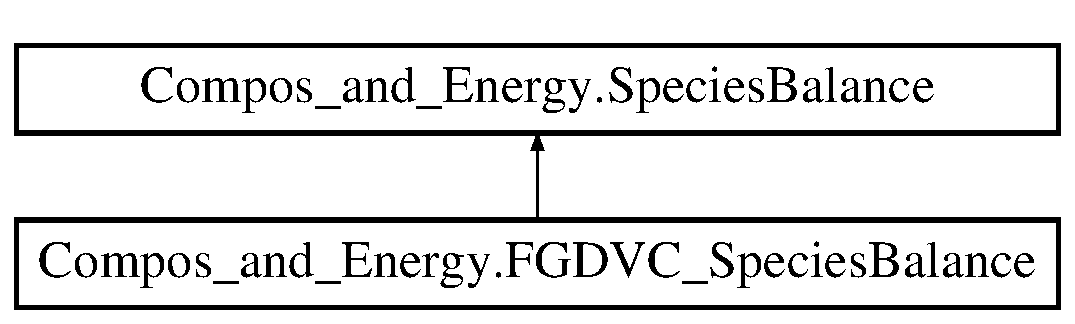
\includegraphics[height=2.000000cm]{classCompos__and__Energy_1_1FGDVC__SpeciesBalance}
\end{center}
\end{figure}
\subsection*{\-Public \-Member \-Functions}
\begin{DoxyCompactItemize}
\item 
\hypertarget{classCompos__and__Energy_1_1FGDVC__SpeciesBalance_ae74f897eb058271f9d11fce7ec511c82}{def {\bfseries \-\_\-\-\_\-init\-\_\-\-\_\-}}\label{classCompos__and__Energy_1_1FGDVC__SpeciesBalance_ae74f897eb058271f9d11fce7ec511c82}

\item 
def \hyperlink{classCompos__and__Energy_1_1SpeciesBalance_a5fec9a8d342543711abe2fc10632efb0}{\-Species\-Index}
\item 
def \hyperlink{classCompos__and__Energy_1_1SpeciesBalance_ae6b9b1a304a5b3686888725624c5e329}{moisture\-Volume\-Fraction}
\item 
def \hyperlink{classCompos__and__Energy_1_1SpeciesBalance_abeff1c726b62ba6c2d32173eb7f51d48}{\-Dulong}
\item 
def \hyperlink{classCompos__and__Energy_1_1SpeciesBalance_a05ae92b73a997e779c64bd2e6386a918}{correct\-U\-A}
\end{DoxyCompactItemize}
\subsection*{\-Public \-Attributes}
\begin{DoxyCompactItemize}
\item 
\hypertarget{classCompos__and__Energy_1_1FGDVC__SpeciesBalance_aa6fbeb442400d9f322d725b48645c4a4}{{\bfseries density\-Dry\-Coal}}\label{classCompos__and__Energy_1_1FGDVC__SpeciesBalance_aa6fbeb442400d9f322d725b48645c4a4}

\item 
\hypertarget{classCompos__and__Energy_1_1FGDVC__SpeciesBalance_afe81cbdce8222489c9d6f2857254d24c}{{\bfseries \-Yields2\-Cols}}\label{classCompos__and__Energy_1_1FGDVC__SpeciesBalance_afe81cbdce8222489c9d6f2857254d24c}

\item 
\hypertarget{classCompos__and__Energy_1_1FGDVC__SpeciesBalance_ae8707824bc19fe728f819f0e4b468992}{{\bfseries \-Cols2\-Yields}}\label{classCompos__and__Energy_1_1FGDVC__SpeciesBalance_ae8707824bc19fe728f819f0e4b468992}

\item 
\hypertarget{classCompos__and__Energy_1_1FGDVC__SpeciesBalance_a4173e5cbd7c8cb79dfa2c1cbac67f8ff}{{\bfseries \-Yields}}\label{classCompos__and__Energy_1_1FGDVC__SpeciesBalance_a4173e5cbd7c8cb79dfa2c1cbac67f8ff}

\item 
\hypertarget{classCompos__and__Energy_1_1FGDVC__SpeciesBalance_aa3e3eca940810e81d44cab414314e906}{{\bfseries \-U\-A\-C}}\label{classCompos__and__Energy_1_1FGDVC__SpeciesBalance_aa3e3eca940810e81d44cab414314e906}

\item 
\hypertarget{classCompos__and__Energy_1_1FGDVC__SpeciesBalance_a26d7171fe63e678f3d4d82e9b3027cbd}{{\bfseries \-U\-A\-H}}\label{classCompos__and__Energy_1_1FGDVC__SpeciesBalance_a26d7171fe63e678f3d4d82e9b3027cbd}

\item 
\hypertarget{classCompos__and__Energy_1_1FGDVC__SpeciesBalance_a6d7538a792df075c4d7c06f52f83869e}{{\bfseries \-U\-A\-N}}\label{classCompos__and__Energy_1_1FGDVC__SpeciesBalance_a6d7538a792df075c4d7c06f52f83869e}

\item 
\hypertarget{classCompos__and__Energy_1_1FGDVC__SpeciesBalance_ab5f7bd829c6e936cf8ae924c52038c20}{{\bfseries \-U\-A\-O}}\label{classCompos__and__Energy_1_1FGDVC__SpeciesBalance_ab5f7bd829c6e936cf8ae924c52038c20}

\item 
\hypertarget{classCompos__and__Energy_1_1FGDVC__SpeciesBalance_a599c435f38f15ca39e10c78c66701df2}{{\bfseries \-U\-A\-S}}\label{classCompos__and__Energy_1_1FGDVC__SpeciesBalance_a599c435f38f15ca39e10c78c66701df2}

\item 
\hypertarget{classCompos__and__Energy_1_1FGDVC__SpeciesBalance_ae3db3cb094567a3f2eaf1c835719198a}{{\bfseries \-P\-A\-V\-M}}\label{classCompos__and__Energy_1_1FGDVC__SpeciesBalance_ae3db3cb094567a3f2eaf1c835719198a}

\item 
\hypertarget{classCompos__and__Energy_1_1FGDVC__SpeciesBalance_ab2aa9b4bcf8227209a02a236435f0afb}{{\bfseries \-P\-A\-F\-C}}\label{classCompos__and__Energy_1_1FGDVC__SpeciesBalance_ab2aa9b4bcf8227209a02a236435f0afb}

\item 
\hypertarget{classCompos__and__Energy_1_1FGDVC__SpeciesBalance_a66de0b97f6dfe92b5f06ea1433e7e056}{{\bfseries \-Char}}\label{classCompos__and__Energy_1_1FGDVC__SpeciesBalance_a66de0b97f6dfe92b5f06ea1433e7e056}

\item 
\hypertarget{classCompos__and__Energy_1_1FGDVC__SpeciesBalance_ac35741f7f74aede9f9f02a869822f25d}{{\bfseries \-C\-O}}\label{classCompos__and__Energy_1_1FGDVC__SpeciesBalance_ac35741f7f74aede9f9f02a869822f25d}

\item 
\hypertarget{classCompos__and__Energy_1_1FGDVC__SpeciesBalance_a989113c4f81191a7ad397a2bc40ff481}{{\bfseries \-C\-O2}}\label{classCompos__and__Energy_1_1FGDVC__SpeciesBalance_a989113c4f81191a7ad397a2bc40ff481}

\item 
\hypertarget{classCompos__and__Energy_1_1FGDVC__SpeciesBalance_acea48a2d58b03402ebbe0495ec80cf93}{{\bfseries \-H2\-O}}\label{classCompos__and__Energy_1_1FGDVC__SpeciesBalance_acea48a2d58b03402ebbe0495ec80cf93}

\item 
\hypertarget{classCompos__and__Energy_1_1FGDVC__SpeciesBalance_ade1a08c6859c18e632d5c2bea272e5f7}{{\bfseries \-C\-H4}}\label{classCompos__and__Energy_1_1FGDVC__SpeciesBalance_ade1a08c6859c18e632d5c2bea272e5f7}

\item 
\hypertarget{classCompos__and__Energy_1_1FGDVC__SpeciesBalance_a30ee4618dcee1ea24cff8b284dde552f}{{\bfseries \-H2}}\label{classCompos__and__Energy_1_1FGDVC__SpeciesBalance_a30ee4618dcee1ea24cff8b284dde552f}

\item 
\hypertarget{classCompos__and__Energy_1_1FGDVC__SpeciesBalance_a8ff55e0b4ddd9f051e132a4b969c18b8}{{\bfseries \-Tar}}\label{classCompos__and__Energy_1_1FGDVC__SpeciesBalance_a8ff55e0b4ddd9f051e132a4b969c18b8}

\item 
\hypertarget{classCompos__and__Energy_1_1FGDVC__SpeciesBalance_afd4b8018c475bdcec14c16ddc5ac2811}{{\bfseries \-L\-H\-Vdaf}}\label{classCompos__and__Energy_1_1FGDVC__SpeciesBalance_afd4b8018c475bdcec14c16ddc5ac2811}

\item 
\hypertarget{classCompos__and__Energy_1_1FGDVC__SpeciesBalance_a04c70dda12807ef0b77d49483b4b5b89}{{\bfseries hf\-Tar}}\label{classCompos__and__Energy_1_1FGDVC__SpeciesBalance_a04c70dda12807ef0b77d49483b4b5b89}

\end{DoxyCompactItemize}
\subsection*{\-Static \-Public \-Attributes}
\begin{DoxyCompactItemize}
\item 
\hypertarget{classCompos__and__Energy_1_1FGDVC__SpeciesBalance_a4696829d0164bb40c9e5205334c46e86}{tuple {\bfseries \-H\-H\-V} = self.\-Dulong()}\label{classCompos__and__Energy_1_1FGDVC__SpeciesBalance_a4696829d0164bb40c9e5205334c46e86}

\item 
\hypertarget{classCompos__and__Energy_1_1FGDVC__SpeciesBalance_a4294e22b98d0497a9d89ea5cc6cbeec9}{tuple {\bfseries char} = self.\-Char$\ast$(1.-\/self.\-P\-Aash)}\label{classCompos__and__Energy_1_1FGDVC__SpeciesBalance_a4294e22b98d0497a9d89ea5cc6cbeec9}

\item 
\hypertarget{classCompos__and__Energy_1_1FGDVC__SpeciesBalance_aa84a0a8f02f9f30916cbabfe7cee3409}{tuple {\bfseries vol} = (1-\/self.\-Char)}\label{classCompos__and__Energy_1_1FGDVC__SpeciesBalance_aa84a0a8f02f9f30916cbabfe7cee3409}

\item 
\hypertarget{classCompos__and__Energy_1_1FGDVC__SpeciesBalance_a72b68b3215acc14ce6e995208dc7b4c1}{int {\bfseries ash} = 100}\label{classCompos__and__Energy_1_1FGDVC__SpeciesBalance_a72b68b3215acc14ce6e995208dc7b4c1}

\item 
\hypertarget{classCompos__and__Energy_1_1SpeciesBalance_a57d64961c8e035bf8087528adf669379}{{\bfseries sum\-U\-A} = self.\-U\-A\-C+self.\-U\-A\-H+self.\-U\-A\-O+self.\-U\-A\-N+self.\-U\-A\-S}\label{classCompos__and__Energy_1_1SpeciesBalance_a57d64961c8e035bf8087528adf669379}

\end{DoxyCompactItemize}


\subsection{\-Detailed \-Description}
\begin{DoxyVerb}This class calculates the Species and the Energy balance for FG-DVC. See the manual for the formulars and more details.\end{DoxyVerb}
 

\subsection{\-Member \-Function \-Documentation}
\hypertarget{classCompos__and__Energy_1_1SpeciesBalance_a05ae92b73a997e779c64bd2e6386a918}{\index{\-Compos\-\_\-and\-\_\-\-Energy\-::\-F\-G\-D\-V\-C\-\_\-\-Species\-Balance@{\-Compos\-\_\-and\-\_\-\-Energy\-::\-F\-G\-D\-V\-C\-\_\-\-Species\-Balance}!correct\-U\-A@{correct\-U\-A}}
\index{correct\-U\-A@{correct\-U\-A}!Compos_and_Energy::FGDVC_SpeciesBalance@{\-Compos\-\_\-and\-\_\-\-Energy\-::\-F\-G\-D\-V\-C\-\_\-\-Species\-Balance}}
\subsubsection[{correct\-U\-A}]{\setlength{\rightskip}{0pt plus 5cm}def {\bf \-Compos\-\_\-and\-\_\-\-Energy.\-Species\-Balance.\-correct\-U\-A} (
\begin{DoxyParamCaption}
\item[{}]{self}
\end{DoxyParamCaption}
)\hspace{0.3cm}{\ttfamily  \mbox{[}inherited\mbox{]}}}}\label{classCompos__and__Energy_1_1SpeciesBalance_a05ae92b73a997e779c64bd2e6386a918}
\begin{DoxyVerb}Scale Ultimate Analysis to have sum=1\end{DoxyVerb}
 \hypertarget{classCompos__and__Energy_1_1SpeciesBalance_abeff1c726b62ba6c2d32173eb7f51d48}{\index{\-Compos\-\_\-and\-\_\-\-Energy\-::\-F\-G\-D\-V\-C\-\_\-\-Species\-Balance@{\-Compos\-\_\-and\-\_\-\-Energy\-::\-F\-G\-D\-V\-C\-\_\-\-Species\-Balance}!\-Dulong@{\-Dulong}}
\index{\-Dulong@{\-Dulong}!Compos_and_Energy::FGDVC_SpeciesBalance@{\-Compos\-\_\-and\-\_\-\-Energy\-::\-F\-G\-D\-V\-C\-\_\-\-Species\-Balance}}
\subsubsection[{\-Dulong}]{\setlength{\rightskip}{0pt plus 5cm}def {\bf \-Compos\-\_\-and\-\_\-\-Energy.\-Species\-Balance.\-Dulong} (
\begin{DoxyParamCaption}
\item[{}]{self}
\end{DoxyParamCaption}
)\hspace{0.3cm}{\ttfamily  \mbox{[}inherited\mbox{]}}}}\label{classCompos__and__Energy_1_1SpeciesBalance_abeff1c726b62ba6c2d32173eb7f51d48}
\begin{DoxyVerb}Uses the Dulong formular to calculate the Higher heating value. The output is in J/kg.\end{DoxyVerb}
 \hypertarget{classCompos__and__Energy_1_1SpeciesBalance_ae6b9b1a304a5b3686888725624c5e329}{\index{\-Compos\-\_\-and\-\_\-\-Energy\-::\-F\-G\-D\-V\-C\-\_\-\-Species\-Balance@{\-Compos\-\_\-and\-\_\-\-Energy\-::\-F\-G\-D\-V\-C\-\_\-\-Species\-Balance}!moisture\-Volume\-Fraction@{moisture\-Volume\-Fraction}}
\index{moisture\-Volume\-Fraction@{moisture\-Volume\-Fraction}!Compos_and_Energy::FGDVC_SpeciesBalance@{\-Compos\-\_\-and\-\_\-\-Energy\-::\-F\-G\-D\-V\-C\-\_\-\-Species\-Balance}}
\subsubsection[{moisture\-Volume\-Fraction}]{\setlength{\rightskip}{0pt plus 5cm}def {\bf \-Compos\-\_\-and\-\_\-\-Energy.\-Species\-Balance.\-moisture\-Volume\-Fraction} (
\begin{DoxyParamCaption}
\item[{}]{self}
\end{DoxyParamCaption}
)\hspace{0.3cm}{\ttfamily  \mbox{[}inherited\mbox{]}}}}\label{classCompos__and__Energy_1_1SpeciesBalance_ae6b9b1a304a5b3686888725624c5e329}
\begin{DoxyVerb}
calculate volume fraction of moisture
\end{DoxyVerb}
 \hypertarget{classCompos__and__Energy_1_1SpeciesBalance_a5fec9a8d342543711abe2fc10632efb0}{\index{\-Compos\-\_\-and\-\_\-\-Energy\-::\-F\-G\-D\-V\-C\-\_\-\-Species\-Balance@{\-Compos\-\_\-and\-\_\-\-Energy\-::\-F\-G\-D\-V\-C\-\_\-\-Species\-Balance}!\-Species\-Index@{\-Species\-Index}}
\index{\-Species\-Index@{\-Species\-Index}!Compos_and_Energy::FGDVC_SpeciesBalance@{\-Compos\-\_\-and\-\_\-\-Energy\-::\-F\-G\-D\-V\-C\-\_\-\-Species\-Balance}}
\subsubsection[{\-Species\-Index}]{\setlength{\rightskip}{0pt plus 5cm}def {\bf \-Compos\-\_\-and\-\_\-\-Energy.\-Species\-Balance.\-Species\-Index} (
\begin{DoxyParamCaption}
\item[{}]{self, }
\item[{}]{species}
\end{DoxyParamCaption}
)\hspace{0.3cm}{\ttfamily  \mbox{[}inherited\mbox{]}}}}\label{classCompos__and__Energy_1_1SpeciesBalance_a5fec9a8d342543711abe2fc10632efb0}
\begin{DoxyVerb}Returns the column number of the input species.\end{DoxyVerb}
 

\-The documentation for this class was generated from the following file\-:\begin{DoxyCompactItemize}
\item 
/home/map/git/pkp/src/\-Compos\-\_\-and\-\_\-\-Energy.\-py\end{DoxyCompactItemize}

\hypertarget{classFitInfo_1_1Fit__one__run}{\section{\-Fit\-Info.\-Fit\-\_\-one\-\_\-run \-Class \-Reference}
\label{classFitInfo_1_1Fit__one__run}\index{\-Fit\-Info.\-Fit\-\_\-one\-\_\-run@{\-Fit\-Info.\-Fit\-\_\-one\-\_\-run}}
}
\subsection*{\-Public \-Member \-Functions}
\begin{DoxyCompactItemize}
\item 
\hypertarget{classFitInfo_1_1Fit__one__run_afaeeadb5a8eb0b8e3027bbd6f4aecec4}{def {\bfseries \-\_\-\-\_\-init\-\_\-\-\_\-}}\label{classFitInfo_1_1Fit__one__run_afaeeadb5a8eb0b8e3027bbd6f4aecec4}

\item 
def \hyperlink{classFitInfo_1_1Fit__one__run_a22e0f9b86db5ab17d84594be261b3f51}{plt\-\_\-\-Input\-Vectors}
\item 
def \hyperlink{classFitInfo_1_1Fit__one__run_ac3755b6b7d3074da8a4d1f2351067fab}{plt\-\_\-\-Yield\-Vs\-Time}
\item 
def \hyperlink{classFitInfo_1_1Fit__one__run_a6ef4ec9d1115393618699b035ea91261}{plt\-\_\-\-Rate\-Vs\-Time}
\item 
def \hyperlink{classFitInfo_1_1Fit__one__run_a474ef41cdcd65bdcc6efd3a0f5a69198}{\-Time}
\item 
def \hyperlink{classFitInfo_1_1Fit__one__run_ac4860413bd4693eb247d73ac64eb13be}{\-Yield}
\item 
def \hyperlink{classFitInfo_1_1Fit__one__run_a225bc2b47046a6630571306161005b5f}{\-Rate}
\item 
def \hyperlink{classFitInfo_1_1Fit__one__run_abdd87a5ecd7a9eafbad662dd5052e452}{\-Mass\-Coal}
\item 
def \hyperlink{classFitInfo_1_1Fit__one__run_af046e7caf8d696baaab86d7fb8d383ba}{\-Mass\-V\-M\-\_\-s}
\item 
def \hyperlink{classFitInfo_1_1Fit__one__run_a18e4a09e916eaab49875d4896806856e}{\-N\-Points}
\item 
def \hyperlink{classFitInfo_1_1Fit__one__run_a1d6a28dfe2ebc03db22b2f13941f8d6f}{\-Rate\-Single\-Spec}
\item 
def \hyperlink{classFitInfo_1_1Fit__one__run_a7d9de59d382b05d6e5f2998fd30eecd7}{\-Species\-Name}
\item 
def \hyperlink{classFitInfo_1_1Fit__one__run_aa86320414c2a97015418ab420e22b03d}{\-Species\-Names}
\item 
def \hyperlink{classFitInfo_1_1Fit__one__run_a009992fd630296ced088620aa3cde5d1}{\-Species\-Index}
\item 
def \hyperlink{classFitInfo_1_1Fit__one__run_a62a341421070dbd08579d07dc455cb83}{\-Dt}
\item 
def \hyperlink{classFitInfo_1_1Fit__one__run_a3a0ca5c2c4ed469e6419848826ed5afa}{\-Dt\-C}
\item 
def \hyperlink{classFitInfo_1_1Fit__one__run_a5000d9d5386ef7f1308f012a7b0f548d}{\-Interpolate}
\item 
def \hyperlink{classFitInfo_1_1Fit__one__run_ab39578a2d9e1295264ecfe29803902f1}{\-Line\-Number\-Max\-Rate}
\item 
def \hyperlink{classFitInfo_1_1Fit__one__run_a3ea2c81143ec30d52e1a3989136da50d}{\-Name}
\end{DoxyCompactItemize}
\subsection*{\-Public \-Attributes}
\begin{DoxyCompactItemize}
\item 
\hypertarget{classFitInfo_1_1Fit__one__run_ac2523fc7cbfc1346537cab9df6a44011}{{\bfseries \-Yields2\-Cols}}\label{classFitInfo_1_1Fit__one__run_ac2523fc7cbfc1346537cab9df6a44011}

\item 
\hypertarget{classFitInfo_1_1Fit__one__run_a035f7a0a99f02cfebd77b713ddda9810}{{\bfseries \-Cols2\-Yields}}\label{classFitInfo_1_1Fit__one__run_a035f7a0a99f02cfebd77b713ddda9810}

\item 
\hypertarget{classFitInfo_1_1Fit__one__run_a37a621b40a56c780a6f9f15d1df324ad}{{\bfseries \-T\-\_\-interpol}}\label{classFitInfo_1_1Fit__one__run_a37a621b40a56c780a6f9f15d1df324ad}

\end{DoxyCompactItemize}


\subsection{\-Detailed \-Description}
\begin{DoxyVerb}Imports from the Result objects the arrays. It provides the fitting objects with the yields and rates over time for the specific species. This class futher offers the option to plot the generated fitting results.\end{DoxyVerb}
 

\subsection{\-Member \-Function \-Documentation}
\hypertarget{classFitInfo_1_1Fit__one__run_a62a341421070dbd08579d07dc455cb83}{\index{\-Fit\-Info\-::\-Fit\-\_\-one\-\_\-run@{\-Fit\-Info\-::\-Fit\-\_\-one\-\_\-run}!\-Dt@{\-Dt}}
\index{\-Dt@{\-Dt}!FitInfo::Fit_one_run@{\-Fit\-Info\-::\-Fit\-\_\-one\-\_\-run}}
\subsubsection[{\-Dt}]{\setlength{\rightskip}{0pt plus 5cm}def {\bf \-Fit\-Info.\-Fit\-\_\-one\-\_\-run.\-Dt} (
\begin{DoxyParamCaption}
\item[{}]{self}
\end{DoxyParamCaption}
)}}\label{classFitInfo_1_1Fit__one__run_a62a341421070dbd08579d07dc455cb83}
\begin{DoxyVerb}Returns the vector with the time steps dt.\end{DoxyVerb}
 \hypertarget{classFitInfo_1_1Fit__one__run_a3a0ca5c2c4ed469e6419848826ed5afa}{\index{\-Fit\-Info\-::\-Fit\-\_\-one\-\_\-run@{\-Fit\-Info\-::\-Fit\-\_\-one\-\_\-run}!\-Dt\-C@{\-Dt\-C}}
\index{\-Dt\-C@{\-Dt\-C}!FitInfo::Fit_one_run@{\-Fit\-Info\-::\-Fit\-\_\-one\-\_\-run}}
\subsubsection[{\-Dt\-C}]{\setlength{\rightskip}{0pt plus 5cm}def {\bf \-Fit\-Info.\-Fit\-\_\-one\-\_\-run.\-Dt\-C} (
\begin{DoxyParamCaption}
\item[{}]{self}
\end{DoxyParamCaption}
)}}\label{classFitInfo_1_1Fit__one__run_a3a0ca5c2c4ed469e6419848826ed5afa}
\begin{DoxyVerb}Returns the vector with the time steps dt_C. This time steps are for points between the original points, so the lenght of this vector is the lenght of the time vector minus one.\end{DoxyVerb}
 \hypertarget{classFitInfo_1_1Fit__one__run_a5000d9d5386ef7f1308f012a7b0f548d}{\index{\-Fit\-Info\-::\-Fit\-\_\-one\-\_\-run@{\-Fit\-Info\-::\-Fit\-\_\-one\-\_\-run}!\-Interpolate@{\-Interpolate}}
\index{\-Interpolate@{\-Interpolate}!FitInfo::Fit_one_run@{\-Fit\-Info\-::\-Fit\-\_\-one\-\_\-run}}
\subsubsection[{\-Interpolate}]{\setlength{\rightskip}{0pt plus 5cm}def {\bf \-Fit\-Info.\-Fit\-\_\-one\-\_\-run.\-Interpolate} (
\begin{DoxyParamCaption}
\item[{}]{self, }
\item[{}]{\-Species}
\end{DoxyParamCaption}
)}}\label{classFitInfo_1_1Fit__one__run_a5000d9d5386ef7f1308f012a7b0f548d}
\begin{DoxyVerb}Outputs the interpolation object (e.g.Species(time)).\end{DoxyVerb}
 \hypertarget{classFitInfo_1_1Fit__one__run_ab39578a2d9e1295264ecfe29803902f1}{\index{\-Fit\-Info\-::\-Fit\-\_\-one\-\_\-run@{\-Fit\-Info\-::\-Fit\-\_\-one\-\_\-run}!\-Line\-Number\-Max\-Rate@{\-Line\-Number\-Max\-Rate}}
\index{\-Line\-Number\-Max\-Rate@{\-Line\-Number\-Max\-Rate}!FitInfo::Fit_one_run@{\-Fit\-Info\-::\-Fit\-\_\-one\-\_\-run}}
\subsubsection[{\-Line\-Number\-Max\-Rate}]{\setlength{\rightskip}{0pt plus 5cm}def {\bf \-Fit\-Info.\-Fit\-\_\-one\-\_\-run.\-Line\-Number\-Max\-Rate} (
\begin{DoxyParamCaption}
\item[{}]{self, }
\item[{}]{\-Species}
\end{DoxyParamCaption}
)}}\label{classFitInfo_1_1Fit__one__run_ab39578a2d9e1295264ecfe29803902f1}
\begin{DoxyVerb}Returns the line with the maximum Rate of the inputted species.\end{DoxyVerb}
 \hypertarget{classFitInfo_1_1Fit__one__run_abdd87a5ecd7a9eafbad662dd5052e452}{\index{\-Fit\-Info\-::\-Fit\-\_\-one\-\_\-run@{\-Fit\-Info\-::\-Fit\-\_\-one\-\_\-run}!\-Mass\-Coal@{\-Mass\-Coal}}
\index{\-Mass\-Coal@{\-Mass\-Coal}!FitInfo::Fit_one_run@{\-Fit\-Info\-::\-Fit\-\_\-one\-\_\-run}}
\subsubsection[{\-Mass\-Coal}]{\setlength{\rightskip}{0pt plus 5cm}def {\bf \-Fit\-Info.\-Fit\-\_\-one\-\_\-run.\-Mass\-Coal} (
\begin{DoxyParamCaption}
\item[{}]{self}
\end{DoxyParamCaption}
)}}\label{classFitInfo_1_1Fit__one__run_abdd87a5ecd7a9eafbad662dd5052e452}
\begin{DoxyVerb}returns the Vector with the solid mass(t)\end{DoxyVerb}
 \hypertarget{classFitInfo_1_1Fit__one__run_af046e7caf8d696baaab86d7fb8d383ba}{\index{\-Fit\-Info\-::\-Fit\-\_\-one\-\_\-run@{\-Fit\-Info\-::\-Fit\-\_\-one\-\_\-run}!\-Mass\-V\-M\-\_\-s@{\-Mass\-V\-M\-\_\-s}}
\index{\-Mass\-V\-M\-\_\-s@{\-Mass\-V\-M\-\_\-s}!FitInfo::Fit_one_run@{\-Fit\-Info\-::\-Fit\-\_\-one\-\_\-run}}
\subsubsection[{\-Mass\-V\-M\-\_\-s}]{\setlength{\rightskip}{0pt plus 5cm}def {\bf \-Fit\-Info.\-Fit\-\_\-one\-\_\-run.\-Mass\-V\-M\-\_\-s} (
\begin{DoxyParamCaption}
\item[{}]{self}
\end{DoxyParamCaption}
)}}\label{classFitInfo_1_1Fit__one__run_af046e7caf8d696baaab86d7fb8d383ba}
\begin{DoxyVerb}Returns the Vector with the mass of the volatile Matter over time\end{DoxyVerb}
 \hypertarget{classFitInfo_1_1Fit__one__run_a3ea2c81143ec30d52e1a3989136da50d}{\index{\-Fit\-Info\-::\-Fit\-\_\-one\-\_\-run@{\-Fit\-Info\-::\-Fit\-\_\-one\-\_\-run}!\-Name@{\-Name}}
\index{\-Name@{\-Name}!FitInfo::Fit_one_run@{\-Fit\-Info\-::\-Fit\-\_\-one\-\_\-run}}
\subsubsection[{\-Name}]{\setlength{\rightskip}{0pt plus 5cm}def {\bf \-Fit\-Info.\-Fit\-\_\-one\-\_\-run.\-Name} (
\begin{DoxyParamCaption}
\item[{}]{self}
\end{DoxyParamCaption}
)}}\label{classFitInfo_1_1Fit__one__run_a3ea2c81143ec30d52e1a3989136da50d}
\begin{DoxyVerb}Returns the Name of the imported Result object (e.g. 'CPD')\end{DoxyVerb}
 \hypertarget{classFitInfo_1_1Fit__one__run_a18e4a09e916eaab49875d4896806856e}{\index{\-Fit\-Info\-::\-Fit\-\_\-one\-\_\-run@{\-Fit\-Info\-::\-Fit\-\_\-one\-\_\-run}!\-N\-Points@{\-N\-Points}}
\index{\-N\-Points@{\-N\-Points}!FitInfo::Fit_one_run@{\-Fit\-Info\-::\-Fit\-\_\-one\-\_\-run}}
\subsubsection[{\-N\-Points}]{\setlength{\rightskip}{0pt plus 5cm}def {\bf \-Fit\-Info.\-Fit\-\_\-one\-\_\-run.\-N\-Points} (
\begin{DoxyParamCaption}
\item[{}]{self}
\end{DoxyParamCaption}
)}}\label{classFitInfo_1_1Fit__one__run_a18e4a09e916eaab49875d4896806856e}
\begin{DoxyVerb}returns number of Points for each species over time. Is equal the number of time points.\end{DoxyVerb}
 \hypertarget{classFitInfo_1_1Fit__one__run_a22e0f9b86db5ab17d84594be261b3f51}{\index{\-Fit\-Info\-::\-Fit\-\_\-one\-\_\-run@{\-Fit\-Info\-::\-Fit\-\_\-one\-\_\-run}!plt\-\_\-\-Input\-Vectors@{plt\-\_\-\-Input\-Vectors}}
\index{plt\-\_\-\-Input\-Vectors@{plt\-\_\-\-Input\-Vectors}!FitInfo::Fit_one_run@{\-Fit\-Info\-::\-Fit\-\_\-one\-\_\-run}}
\subsubsection[{plt\-\_\-\-Input\-Vectors}]{\setlength{\rightskip}{0pt plus 5cm}def {\bf \-Fit\-Info.\-Fit\-\_\-one\-\_\-run.\-plt\-\_\-\-Input\-Vectors} (
\begin{DoxyParamCaption}
\item[{}]{self, }
\item[{}]{x\-Vector, }
\item[{}]{y1\-Vector, }
\item[{}]{y2\-Vector, }
\item[{}]{y3\-Vector, }
\item[{}]{y4\-Vector, }
\item[{}]{y1\-Name, }
\item[{}]{y2\-Name, }
\item[{}]{y3\-Name, }
\item[{}]{y4\-Name}
\end{DoxyParamCaption}
)}}\label{classFitInfo_1_1Fit__one__run_a22e0f9b86db5ab17d84594be261b3f51}
\begin{DoxyVerb}Plots the y input Vectors vs. the x input vector.\end{DoxyVerb}
 \hypertarget{classFitInfo_1_1Fit__one__run_a6ef4ec9d1115393618699b035ea91261}{\index{\-Fit\-Info\-::\-Fit\-\_\-one\-\_\-run@{\-Fit\-Info\-::\-Fit\-\_\-one\-\_\-run}!plt\-\_\-\-Rate\-Vs\-Time@{plt\-\_\-\-Rate\-Vs\-Time}}
\index{plt\-\_\-\-Rate\-Vs\-Time@{plt\-\_\-\-Rate\-Vs\-Time}!FitInfo::Fit_one_run@{\-Fit\-Info\-::\-Fit\-\_\-one\-\_\-run}}
\subsubsection[{plt\-\_\-\-Rate\-Vs\-Time}]{\setlength{\rightskip}{0pt plus 5cm}def {\bf \-Fit\-Info.\-Fit\-\_\-one\-\_\-run.\-plt\-\_\-\-Rate\-Vs\-Time} (
\begin{DoxyParamCaption}
\item[{}]{self, }
\item[{}]{\-Column\-Number}
\end{DoxyParamCaption}
)}}\label{classFitInfo_1_1Fit__one__run_a6ef4ec9d1115393618699b035ea91261}
\begin{DoxyVerb}Plots the original rates output of the pyrolysis program (as e.g. CPD) of the species marke with the columns number\end{DoxyVerb}
 \hypertarget{classFitInfo_1_1Fit__one__run_ac3755b6b7d3074da8a4d1f2351067fab}{\index{\-Fit\-Info\-::\-Fit\-\_\-one\-\_\-run@{\-Fit\-Info\-::\-Fit\-\_\-one\-\_\-run}!plt\-\_\-\-Yield\-Vs\-Time@{plt\-\_\-\-Yield\-Vs\-Time}}
\index{plt\-\_\-\-Yield\-Vs\-Time@{plt\-\_\-\-Yield\-Vs\-Time}!FitInfo::Fit_one_run@{\-Fit\-Info\-::\-Fit\-\_\-one\-\_\-run}}
\subsubsection[{plt\-\_\-\-Yield\-Vs\-Time}]{\setlength{\rightskip}{0pt plus 5cm}def {\bf \-Fit\-Info.\-Fit\-\_\-one\-\_\-run.\-plt\-\_\-\-Yield\-Vs\-Time} (
\begin{DoxyParamCaption}
\item[{}]{self, }
\item[{}]{\-Column\-Number}
\end{DoxyParamCaption}
)}}\label{classFitInfo_1_1Fit__one__run_ac3755b6b7d3074da8a4d1f2351067fab}
\begin{DoxyVerb}Plots the original yield output of the pyrolysis program (as e.g. CPD) of the species marke with the columns number\end{DoxyVerb}
 \hypertarget{classFitInfo_1_1Fit__one__run_a225bc2b47046a6630571306161005b5f}{\index{\-Fit\-Info\-::\-Fit\-\_\-one\-\_\-run@{\-Fit\-Info\-::\-Fit\-\_\-one\-\_\-run}!\-Rate@{\-Rate}}
\index{\-Rate@{\-Rate}!FitInfo::Fit_one_run@{\-Fit\-Info\-::\-Fit\-\_\-one\-\_\-run}}
\subsubsection[{\-Rate}]{\setlength{\rightskip}{0pt plus 5cm}def {\bf \-Fit\-Info.\-Fit\-\_\-one\-\_\-run.\-Rate} (
\begin{DoxyParamCaption}
\item[{}]{self, }
\item[{}]{species}
\end{DoxyParamCaption}
)}}\label{classFitInfo_1_1Fit__one__run_a225bc2b47046a6630571306161005b5f}
\begin{DoxyVerb}Returns the Vector of the species rate(t). The species can be inputted with the Column number (integer) or the name corresponding to the dictionary saved in the result class (string).\end{DoxyVerb}
 \hypertarget{classFitInfo_1_1Fit__one__run_a1d6a28dfe2ebc03db22b2f13941f8d6f}{\index{\-Fit\-Info\-::\-Fit\-\_\-one\-\_\-run@{\-Fit\-Info\-::\-Fit\-\_\-one\-\_\-run}!\-Rate\-Single\-Spec@{\-Rate\-Single\-Spec}}
\index{\-Rate\-Single\-Spec@{\-Rate\-Single\-Spec}!FitInfo::Fit_one_run@{\-Fit\-Info\-::\-Fit\-\_\-one\-\_\-run}}
\subsubsection[{\-Rate\-Single\-Spec}]{\setlength{\rightskip}{0pt plus 5cm}def {\bf \-Fit\-Info.\-Fit\-\_\-one\-\_\-run.\-Rate\-Single\-Spec} (
\begin{DoxyParamCaption}
\item[{}]{self, }
\item[{}]{\-Name\-Species}
\end{DoxyParamCaption}
)}}\label{classFitInfo_1_1Fit__one__run_a1d6a28dfe2ebc03db22b2f13941f8d6f}
\begin{DoxyVerb}Returns the Rate of the species (inputted as string) by calculate it from the yields by using a CDS\end{DoxyVerb}
 \hypertarget{classFitInfo_1_1Fit__one__run_a009992fd630296ced088620aa3cde5d1}{\index{\-Fit\-Info\-::\-Fit\-\_\-one\-\_\-run@{\-Fit\-Info\-::\-Fit\-\_\-one\-\_\-run}!\-Species\-Index@{\-Species\-Index}}
\index{\-Species\-Index@{\-Species\-Index}!FitInfo::Fit_one_run@{\-Fit\-Info\-::\-Fit\-\_\-one\-\_\-run}}
\subsubsection[{\-Species\-Index}]{\setlength{\rightskip}{0pt plus 5cm}def {\bf \-Fit\-Info.\-Fit\-\_\-one\-\_\-run.\-Species\-Index} (
\begin{DoxyParamCaption}
\item[{}]{self, }
\item[{}]{species}
\end{DoxyParamCaption}
)}}\label{classFitInfo_1_1Fit__one__run_a009992fd630296ced088620aa3cde5d1}
\begin{DoxyVerb}Returns the species column number (integer) of the recieved species name (string)\end{DoxyVerb}
 \hypertarget{classFitInfo_1_1Fit__one__run_a7d9de59d382b05d6e5f2998fd30eecd7}{\index{\-Fit\-Info\-::\-Fit\-\_\-one\-\_\-run@{\-Fit\-Info\-::\-Fit\-\_\-one\-\_\-run}!\-Species\-Name@{\-Species\-Name}}
\index{\-Species\-Name@{\-Species\-Name}!FitInfo::Fit_one_run@{\-Fit\-Info\-::\-Fit\-\_\-one\-\_\-run}}
\subsubsection[{\-Species\-Name}]{\setlength{\rightskip}{0pt plus 5cm}def {\bf \-Fit\-Info.\-Fit\-\_\-one\-\_\-run.\-Species\-Name} (
\begin{DoxyParamCaption}
\item[{}]{self, }
\item[{}]{\-Column\-Number}
\end{DoxyParamCaption}
)}}\label{classFitInfo_1_1Fit__one__run_a7d9de59d382b05d6e5f2998fd30eecd7}
\begin{DoxyVerb}Returns the species name (string) of the recieved column number (integer)\end{DoxyVerb}
 \hypertarget{classFitInfo_1_1Fit__one__run_aa86320414c2a97015418ab420e22b03d}{\index{\-Fit\-Info\-::\-Fit\-\_\-one\-\_\-run@{\-Fit\-Info\-::\-Fit\-\_\-one\-\_\-run}!\-Species\-Names@{\-Species\-Names}}
\index{\-Species\-Names@{\-Species\-Names}!FitInfo::Fit_one_run@{\-Fit\-Info\-::\-Fit\-\_\-one\-\_\-run}}
\subsubsection[{\-Species\-Names}]{\setlength{\rightskip}{0pt plus 5cm}def {\bf \-Fit\-Info.\-Fit\-\_\-one\-\_\-run.\-Species\-Names} (
\begin{DoxyParamCaption}
\item[{}]{self}
\end{DoxyParamCaption}
)}}\label{classFitInfo_1_1Fit__one__run_aa86320414c2a97015418ab420e22b03d}
\begin{DoxyVerb}Returns a list with all species names (including time and temperature).\end{DoxyVerb}
 \hypertarget{classFitInfo_1_1Fit__one__run_a474ef41cdcd65bdcc6efd3a0f5a69198}{\index{\-Fit\-Info\-::\-Fit\-\_\-one\-\_\-run@{\-Fit\-Info\-::\-Fit\-\_\-one\-\_\-run}!\-Time@{\-Time}}
\index{\-Time@{\-Time}!FitInfo::Fit_one_run@{\-Fit\-Info\-::\-Fit\-\_\-one\-\_\-run}}
\subsubsection[{\-Time}]{\setlength{\rightskip}{0pt plus 5cm}def {\bf \-Fit\-Info.\-Fit\-\_\-one\-\_\-run.\-Time} (
\begin{DoxyParamCaption}
\item[{}]{self}
\end{DoxyParamCaption}
)}}\label{classFitInfo_1_1Fit__one__run_a474ef41cdcd65bdcc6efd3a0f5a69198}
\begin{DoxyVerb}Returns the time vector\end{DoxyVerb}
 \hypertarget{classFitInfo_1_1Fit__one__run_ac4860413bd4693eb247d73ac64eb13be}{\index{\-Fit\-Info\-::\-Fit\-\_\-one\-\_\-run@{\-Fit\-Info\-::\-Fit\-\_\-one\-\_\-run}!\-Yield@{\-Yield}}
\index{\-Yield@{\-Yield}!FitInfo::Fit_one_run@{\-Fit\-Info\-::\-Fit\-\_\-one\-\_\-run}}
\subsubsection[{\-Yield}]{\setlength{\rightskip}{0pt plus 5cm}def {\bf \-Fit\-Info.\-Fit\-\_\-one\-\_\-run.\-Yield} (
\begin{DoxyParamCaption}
\item[{}]{self, }
\item[{}]{species}
\end{DoxyParamCaption}
)}}\label{classFitInfo_1_1Fit__one__run_ac4860413bd4693eb247d73ac64eb13be}
\begin{DoxyVerb}Returns the Vector of the species yield(t). The species can be inputted with the Column number (integer) or the name corresponding to the dictionary saved in the result class (string).\end{DoxyVerb}
 

\-The documentation for this class was generated from the following file\-:\begin{DoxyCompactItemize}
\item 
/home/map/git/pkp/src/\-Fit\-Info.\-py\end{DoxyCompactItemize}

\hypertarget{classFit__one__run_1_1Fit__one__run}{\section{\-Fit\-\_\-one\-\_\-run.\-Fit\-\_\-one\-\_\-run \-Class \-Reference}
\label{classFit__one__run_1_1Fit__one__run}\index{\-Fit\-\_\-one\-\_\-run.\-Fit\-\_\-one\-\_\-run@{\-Fit\-\_\-one\-\_\-run.\-Fit\-\_\-one\-\_\-run}}
}
\subsection*{\-Public \-Member \-Functions}
\begin{DoxyCompactItemize}
\item 
\hypertarget{classFit__one__run_1_1Fit__one__run_a026307f8059de3eaed0e0f30c213688e}{def {\bfseries \-\_\-\-\_\-init\-\_\-\-\_\-}}\label{classFit__one__run_1_1Fit__one__run_a026307f8059de3eaed0e0f30c213688e}

\item 
def \hyperlink{classFit__one__run_1_1Fit__one__run_a8f7f8188c2c37135e67632982964f34a}{plt\-\_\-\-Input\-Vectors}
\item 
def \hyperlink{classFit__one__run_1_1Fit__one__run_a6382bd698c58a57b0748ab459317ede0}{plt\-\_\-\-Yield\-Vs\-Time}
\item 
def \hyperlink{classFit__one__run_1_1Fit__one__run_aef2de6c940020edda5383c9dc0a24759}{plt\-\_\-\-Rate\-Vs\-Time}
\item 
def \hyperlink{classFit__one__run_1_1Fit__one__run_a87ccadc0e52128cc37a19b6032bc1583}{\-Time}
\item 
def \hyperlink{classFit__one__run_1_1Fit__one__run_a94a16b13e2eb75309f0cfd403a7e1047}{\-Yield}
\item 
def \hyperlink{classFit__one__run_1_1Fit__one__run_ac20ff79e8a10d41e8b39cfe15d18f423}{\-Rate}
\item 
def \hyperlink{classFit__one__run_1_1Fit__one__run_a21ec33c24095df5a6450a49a23fa6c8b}{\-Mass\-Coal}
\item 
def \hyperlink{classFit__one__run_1_1Fit__one__run_a606502eebf1f5f28308d3264ff6ce72a}{\-Mass\-V\-M\-\_\-s}
\item 
def \hyperlink{classFit__one__run_1_1Fit__one__run_ab737a97d00c7f40f240560776d1387d5}{\-N\-Points}
\item 
def \hyperlink{classFit__one__run_1_1Fit__one__run_ac30615dce69cf5bd8362ad04a6b2a725}{\-Rate\-Single\-Spec}
\item 
def \hyperlink{classFit__one__run_1_1Fit__one__run_a43b56556c25342482d01b717ddf2e813}{\-Species\-Name}
\item 
def \hyperlink{classFit__one__run_1_1Fit__one__run_ae41e258087d0ef31240ff4ff7cfbb0e7}{\-Species\-Names}
\item 
def \hyperlink{classFit__one__run_1_1Fit__one__run_a8bd23b5cea9a2b4a47d02a4bd8a321b9}{\-Species\-Index}
\item 
def \hyperlink{classFit__one__run_1_1Fit__one__run_a6886d23160b83d181923b4c92bf1bf21}{\-Dt}
\item 
def \hyperlink{classFit__one__run_1_1Fit__one__run_a23124d6b66b984d86c499f6c38fb9d3a}{\-Dt\-C}
\item 
def \hyperlink{classFit__one__run_1_1Fit__one__run_ad83729d5ab493caa0ae5c69b90fc28d1}{\-Interpolate}
\item 
def \hyperlink{classFit__one__run_1_1Fit__one__run_a54698580f9548b276eb6b058de7eda00}{\-Line\-Number\-Max\-Rate}
\item 
def \hyperlink{classFit__one__run_1_1Fit__one__run_ac471c563b5841ba5a9463d3f715579c8}{\-Name}
\end{DoxyCompactItemize}
\subsection*{\-Public \-Attributes}
\begin{DoxyCompactItemize}
\item 
\hypertarget{classFit__one__run_1_1Fit__one__run_acf67bf83bc9f52da3016c0a3ac4e7d6e}{{\bfseries \-Yields2\-Cols}}\label{classFit__one__run_1_1Fit__one__run_acf67bf83bc9f52da3016c0a3ac4e7d6e}

\item 
\hypertarget{classFit__one__run_1_1Fit__one__run_a8ee791dadf161472873fcc3285b8b880}{{\bfseries \-Cols2\-Yields}}\label{classFit__one__run_1_1Fit__one__run_a8ee791dadf161472873fcc3285b8b880}

\item 
\hypertarget{classFit__one__run_1_1Fit__one__run_a408a65ffcdf4c28001ef91bf534ae05a}{{\bfseries \-T\-\_\-interpol}}\label{classFit__one__run_1_1Fit__one__run_a408a65ffcdf4c28001ef91bf534ae05a}

\end{DoxyCompactItemize}


\subsection{\-Detailed \-Description}
\begin{DoxyVerb}Imports from the Result objects the arrays. It provides the fitting objects with the yields and rates over time for the specific species. This class futher offers the option to plot the generated fitting results.\end{DoxyVerb}
 

\subsection{\-Member \-Function \-Documentation}
\hypertarget{classFit__one__run_1_1Fit__one__run_a6886d23160b83d181923b4c92bf1bf21}{\index{\-Fit\-\_\-one\-\_\-run\-::\-Fit\-\_\-one\-\_\-run@{\-Fit\-\_\-one\-\_\-run\-::\-Fit\-\_\-one\-\_\-run}!\-Dt@{\-Dt}}
\index{\-Dt@{\-Dt}!Fit_one_run::Fit_one_run@{\-Fit\-\_\-one\-\_\-run\-::\-Fit\-\_\-one\-\_\-run}}
\subsubsection[{\-Dt}]{\setlength{\rightskip}{0pt plus 5cm}def {\bf \-Fit\-\_\-one\-\_\-run.\-Fit\-\_\-one\-\_\-run.\-Dt} (
\begin{DoxyParamCaption}
\item[{}]{self}
\end{DoxyParamCaption}
)}}\label{classFit__one__run_1_1Fit__one__run_a6886d23160b83d181923b4c92bf1bf21}
\begin{DoxyVerb}Returns the vector with the time steps dt.\end{DoxyVerb}
 \hypertarget{classFit__one__run_1_1Fit__one__run_a23124d6b66b984d86c499f6c38fb9d3a}{\index{\-Fit\-\_\-one\-\_\-run\-::\-Fit\-\_\-one\-\_\-run@{\-Fit\-\_\-one\-\_\-run\-::\-Fit\-\_\-one\-\_\-run}!\-Dt\-C@{\-Dt\-C}}
\index{\-Dt\-C@{\-Dt\-C}!Fit_one_run::Fit_one_run@{\-Fit\-\_\-one\-\_\-run\-::\-Fit\-\_\-one\-\_\-run}}
\subsubsection[{\-Dt\-C}]{\setlength{\rightskip}{0pt plus 5cm}def {\bf \-Fit\-\_\-one\-\_\-run.\-Fit\-\_\-one\-\_\-run.\-Dt\-C} (
\begin{DoxyParamCaption}
\item[{}]{self}
\end{DoxyParamCaption}
)}}\label{classFit__one__run_1_1Fit__one__run_a23124d6b66b984d86c499f6c38fb9d3a}
\begin{DoxyVerb}Returns the vector with the time steps dt_C. This time steps are for points between the original points, so the lenght of this vector is the lenght of the time vector minus one.\end{DoxyVerb}
 \hypertarget{classFit__one__run_1_1Fit__one__run_ad83729d5ab493caa0ae5c69b90fc28d1}{\index{\-Fit\-\_\-one\-\_\-run\-::\-Fit\-\_\-one\-\_\-run@{\-Fit\-\_\-one\-\_\-run\-::\-Fit\-\_\-one\-\_\-run}!\-Interpolate@{\-Interpolate}}
\index{\-Interpolate@{\-Interpolate}!Fit_one_run::Fit_one_run@{\-Fit\-\_\-one\-\_\-run\-::\-Fit\-\_\-one\-\_\-run}}
\subsubsection[{\-Interpolate}]{\setlength{\rightskip}{0pt plus 5cm}def {\bf \-Fit\-\_\-one\-\_\-run.\-Fit\-\_\-one\-\_\-run.\-Interpolate} (
\begin{DoxyParamCaption}
\item[{}]{self, }
\item[{}]{\-Species}
\end{DoxyParamCaption}
)}}\label{classFit__one__run_1_1Fit__one__run_ad83729d5ab493caa0ae5c69b90fc28d1}
\begin{DoxyVerb}Outputs the interpolation object (e.g.Species(time)).\end{DoxyVerb}
 \hypertarget{classFit__one__run_1_1Fit__one__run_a54698580f9548b276eb6b058de7eda00}{\index{\-Fit\-\_\-one\-\_\-run\-::\-Fit\-\_\-one\-\_\-run@{\-Fit\-\_\-one\-\_\-run\-::\-Fit\-\_\-one\-\_\-run}!\-Line\-Number\-Max\-Rate@{\-Line\-Number\-Max\-Rate}}
\index{\-Line\-Number\-Max\-Rate@{\-Line\-Number\-Max\-Rate}!Fit_one_run::Fit_one_run@{\-Fit\-\_\-one\-\_\-run\-::\-Fit\-\_\-one\-\_\-run}}
\subsubsection[{\-Line\-Number\-Max\-Rate}]{\setlength{\rightskip}{0pt plus 5cm}def {\bf \-Fit\-\_\-one\-\_\-run.\-Fit\-\_\-one\-\_\-run.\-Line\-Number\-Max\-Rate} (
\begin{DoxyParamCaption}
\item[{}]{self, }
\item[{}]{\-Species}
\end{DoxyParamCaption}
)}}\label{classFit__one__run_1_1Fit__one__run_a54698580f9548b276eb6b058de7eda00}
\begin{DoxyVerb}Returns the line with the maximum Rate of the inputted species.\end{DoxyVerb}
 \hypertarget{classFit__one__run_1_1Fit__one__run_a21ec33c24095df5a6450a49a23fa6c8b}{\index{\-Fit\-\_\-one\-\_\-run\-::\-Fit\-\_\-one\-\_\-run@{\-Fit\-\_\-one\-\_\-run\-::\-Fit\-\_\-one\-\_\-run}!\-Mass\-Coal@{\-Mass\-Coal}}
\index{\-Mass\-Coal@{\-Mass\-Coal}!Fit_one_run::Fit_one_run@{\-Fit\-\_\-one\-\_\-run\-::\-Fit\-\_\-one\-\_\-run}}
\subsubsection[{\-Mass\-Coal}]{\setlength{\rightskip}{0pt plus 5cm}def {\bf \-Fit\-\_\-one\-\_\-run.\-Fit\-\_\-one\-\_\-run.\-Mass\-Coal} (
\begin{DoxyParamCaption}
\item[{}]{self}
\end{DoxyParamCaption}
)}}\label{classFit__one__run_1_1Fit__one__run_a21ec33c24095df5a6450a49a23fa6c8b}
\begin{DoxyVerb}returns the Vector with the solid mass(t)\end{DoxyVerb}
 \hypertarget{classFit__one__run_1_1Fit__one__run_a606502eebf1f5f28308d3264ff6ce72a}{\index{\-Fit\-\_\-one\-\_\-run\-::\-Fit\-\_\-one\-\_\-run@{\-Fit\-\_\-one\-\_\-run\-::\-Fit\-\_\-one\-\_\-run}!\-Mass\-V\-M\-\_\-s@{\-Mass\-V\-M\-\_\-s}}
\index{\-Mass\-V\-M\-\_\-s@{\-Mass\-V\-M\-\_\-s}!Fit_one_run::Fit_one_run@{\-Fit\-\_\-one\-\_\-run\-::\-Fit\-\_\-one\-\_\-run}}
\subsubsection[{\-Mass\-V\-M\-\_\-s}]{\setlength{\rightskip}{0pt plus 5cm}def {\bf \-Fit\-\_\-one\-\_\-run.\-Fit\-\_\-one\-\_\-run.\-Mass\-V\-M\-\_\-s} (
\begin{DoxyParamCaption}
\item[{}]{self}
\end{DoxyParamCaption}
)}}\label{classFit__one__run_1_1Fit__one__run_a606502eebf1f5f28308d3264ff6ce72a}
\begin{DoxyVerb}Returns the Vector with the mass of the volatile Matter over time\end{DoxyVerb}
 \hypertarget{classFit__one__run_1_1Fit__one__run_ac471c563b5841ba5a9463d3f715579c8}{\index{\-Fit\-\_\-one\-\_\-run\-::\-Fit\-\_\-one\-\_\-run@{\-Fit\-\_\-one\-\_\-run\-::\-Fit\-\_\-one\-\_\-run}!\-Name@{\-Name}}
\index{\-Name@{\-Name}!Fit_one_run::Fit_one_run@{\-Fit\-\_\-one\-\_\-run\-::\-Fit\-\_\-one\-\_\-run}}
\subsubsection[{\-Name}]{\setlength{\rightskip}{0pt plus 5cm}def {\bf \-Fit\-\_\-one\-\_\-run.\-Fit\-\_\-one\-\_\-run.\-Name} (
\begin{DoxyParamCaption}
\item[{}]{self}
\end{DoxyParamCaption}
)}}\label{classFit__one__run_1_1Fit__one__run_ac471c563b5841ba5a9463d3f715579c8}
\begin{DoxyVerb}Returns the Name of the imported Result object (e.g. 'CPD')\end{DoxyVerb}
 \hypertarget{classFit__one__run_1_1Fit__one__run_ab737a97d00c7f40f240560776d1387d5}{\index{\-Fit\-\_\-one\-\_\-run\-::\-Fit\-\_\-one\-\_\-run@{\-Fit\-\_\-one\-\_\-run\-::\-Fit\-\_\-one\-\_\-run}!\-N\-Points@{\-N\-Points}}
\index{\-N\-Points@{\-N\-Points}!Fit_one_run::Fit_one_run@{\-Fit\-\_\-one\-\_\-run\-::\-Fit\-\_\-one\-\_\-run}}
\subsubsection[{\-N\-Points}]{\setlength{\rightskip}{0pt plus 5cm}def {\bf \-Fit\-\_\-one\-\_\-run.\-Fit\-\_\-one\-\_\-run.\-N\-Points} (
\begin{DoxyParamCaption}
\item[{}]{self}
\end{DoxyParamCaption}
)}}\label{classFit__one__run_1_1Fit__one__run_ab737a97d00c7f40f240560776d1387d5}
\begin{DoxyVerb}returns number of Points for each species over time. Is equal the number of time points.\end{DoxyVerb}
 \hypertarget{classFit__one__run_1_1Fit__one__run_a8f7f8188c2c37135e67632982964f34a}{\index{\-Fit\-\_\-one\-\_\-run\-::\-Fit\-\_\-one\-\_\-run@{\-Fit\-\_\-one\-\_\-run\-::\-Fit\-\_\-one\-\_\-run}!plt\-\_\-\-Input\-Vectors@{plt\-\_\-\-Input\-Vectors}}
\index{plt\-\_\-\-Input\-Vectors@{plt\-\_\-\-Input\-Vectors}!Fit_one_run::Fit_one_run@{\-Fit\-\_\-one\-\_\-run\-::\-Fit\-\_\-one\-\_\-run}}
\subsubsection[{plt\-\_\-\-Input\-Vectors}]{\setlength{\rightskip}{0pt plus 5cm}def {\bf \-Fit\-\_\-one\-\_\-run.\-Fit\-\_\-one\-\_\-run.\-plt\-\_\-\-Input\-Vectors} (
\begin{DoxyParamCaption}
\item[{}]{self, }
\item[{}]{x\-Vector, }
\item[{}]{y1\-Vector, }
\item[{}]{y2\-Vector, }
\item[{}]{y3\-Vector, }
\item[{}]{y4\-Vector, }
\item[{}]{y1\-Name, }
\item[{}]{y2\-Name, }
\item[{}]{y3\-Name, }
\item[{}]{y4\-Name}
\end{DoxyParamCaption}
)}}\label{classFit__one__run_1_1Fit__one__run_a8f7f8188c2c37135e67632982964f34a}
\begin{DoxyVerb}Plots the y input Vectors vs. the x input vector.\end{DoxyVerb}
 \hypertarget{classFit__one__run_1_1Fit__one__run_aef2de6c940020edda5383c9dc0a24759}{\index{\-Fit\-\_\-one\-\_\-run\-::\-Fit\-\_\-one\-\_\-run@{\-Fit\-\_\-one\-\_\-run\-::\-Fit\-\_\-one\-\_\-run}!plt\-\_\-\-Rate\-Vs\-Time@{plt\-\_\-\-Rate\-Vs\-Time}}
\index{plt\-\_\-\-Rate\-Vs\-Time@{plt\-\_\-\-Rate\-Vs\-Time}!Fit_one_run::Fit_one_run@{\-Fit\-\_\-one\-\_\-run\-::\-Fit\-\_\-one\-\_\-run}}
\subsubsection[{plt\-\_\-\-Rate\-Vs\-Time}]{\setlength{\rightskip}{0pt plus 5cm}def {\bf \-Fit\-\_\-one\-\_\-run.\-Fit\-\_\-one\-\_\-run.\-plt\-\_\-\-Rate\-Vs\-Time} (
\begin{DoxyParamCaption}
\item[{}]{self, }
\item[{}]{\-Column\-Number}
\end{DoxyParamCaption}
)}}\label{classFit__one__run_1_1Fit__one__run_aef2de6c940020edda5383c9dc0a24759}
\begin{DoxyVerb}Plots the original rates output of the pyrolysis program (as e.g. CPD) of the species marke with the columns number\end{DoxyVerb}
 \hypertarget{classFit__one__run_1_1Fit__one__run_a6382bd698c58a57b0748ab459317ede0}{\index{\-Fit\-\_\-one\-\_\-run\-::\-Fit\-\_\-one\-\_\-run@{\-Fit\-\_\-one\-\_\-run\-::\-Fit\-\_\-one\-\_\-run}!plt\-\_\-\-Yield\-Vs\-Time@{plt\-\_\-\-Yield\-Vs\-Time}}
\index{plt\-\_\-\-Yield\-Vs\-Time@{plt\-\_\-\-Yield\-Vs\-Time}!Fit_one_run::Fit_one_run@{\-Fit\-\_\-one\-\_\-run\-::\-Fit\-\_\-one\-\_\-run}}
\subsubsection[{plt\-\_\-\-Yield\-Vs\-Time}]{\setlength{\rightskip}{0pt plus 5cm}def {\bf \-Fit\-\_\-one\-\_\-run.\-Fit\-\_\-one\-\_\-run.\-plt\-\_\-\-Yield\-Vs\-Time} (
\begin{DoxyParamCaption}
\item[{}]{self, }
\item[{}]{\-Column\-Number}
\end{DoxyParamCaption}
)}}\label{classFit__one__run_1_1Fit__one__run_a6382bd698c58a57b0748ab459317ede0}
\begin{DoxyVerb}Plots the original yield output of the pyrolysis program (as e.g. CPD) of the species marke with the columns number\end{DoxyVerb}
 \hypertarget{classFit__one__run_1_1Fit__one__run_ac20ff79e8a10d41e8b39cfe15d18f423}{\index{\-Fit\-\_\-one\-\_\-run\-::\-Fit\-\_\-one\-\_\-run@{\-Fit\-\_\-one\-\_\-run\-::\-Fit\-\_\-one\-\_\-run}!\-Rate@{\-Rate}}
\index{\-Rate@{\-Rate}!Fit_one_run::Fit_one_run@{\-Fit\-\_\-one\-\_\-run\-::\-Fit\-\_\-one\-\_\-run}}
\subsubsection[{\-Rate}]{\setlength{\rightskip}{0pt plus 5cm}def {\bf \-Fit\-\_\-one\-\_\-run.\-Fit\-\_\-one\-\_\-run.\-Rate} (
\begin{DoxyParamCaption}
\item[{}]{self, }
\item[{}]{species}
\end{DoxyParamCaption}
)}}\label{classFit__one__run_1_1Fit__one__run_ac20ff79e8a10d41e8b39cfe15d18f423}
\begin{DoxyVerb}Returns the Vector of the species rate(t). The species can be inputted with the Column number (integer) or the name corresponding to the dictionary saved in the result class (string).\end{DoxyVerb}
 \hypertarget{classFit__one__run_1_1Fit__one__run_ac30615dce69cf5bd8362ad04a6b2a725}{\index{\-Fit\-\_\-one\-\_\-run\-::\-Fit\-\_\-one\-\_\-run@{\-Fit\-\_\-one\-\_\-run\-::\-Fit\-\_\-one\-\_\-run}!\-Rate\-Single\-Spec@{\-Rate\-Single\-Spec}}
\index{\-Rate\-Single\-Spec@{\-Rate\-Single\-Spec}!Fit_one_run::Fit_one_run@{\-Fit\-\_\-one\-\_\-run\-::\-Fit\-\_\-one\-\_\-run}}
\subsubsection[{\-Rate\-Single\-Spec}]{\setlength{\rightskip}{0pt plus 5cm}def {\bf \-Fit\-\_\-one\-\_\-run.\-Fit\-\_\-one\-\_\-run.\-Rate\-Single\-Spec} (
\begin{DoxyParamCaption}
\item[{}]{self, }
\item[{}]{\-Name\-Species}
\end{DoxyParamCaption}
)}}\label{classFit__one__run_1_1Fit__one__run_ac30615dce69cf5bd8362ad04a6b2a725}
\begin{DoxyVerb}Returns the Rate of the species (inputted as string) by calculate it from the yields by using a CDS\end{DoxyVerb}
 \hypertarget{classFit__one__run_1_1Fit__one__run_a8bd23b5cea9a2b4a47d02a4bd8a321b9}{\index{\-Fit\-\_\-one\-\_\-run\-::\-Fit\-\_\-one\-\_\-run@{\-Fit\-\_\-one\-\_\-run\-::\-Fit\-\_\-one\-\_\-run}!\-Species\-Index@{\-Species\-Index}}
\index{\-Species\-Index@{\-Species\-Index}!Fit_one_run::Fit_one_run@{\-Fit\-\_\-one\-\_\-run\-::\-Fit\-\_\-one\-\_\-run}}
\subsubsection[{\-Species\-Index}]{\setlength{\rightskip}{0pt plus 5cm}def {\bf \-Fit\-\_\-one\-\_\-run.\-Fit\-\_\-one\-\_\-run.\-Species\-Index} (
\begin{DoxyParamCaption}
\item[{}]{self, }
\item[{}]{species}
\end{DoxyParamCaption}
)}}\label{classFit__one__run_1_1Fit__one__run_a8bd23b5cea9a2b4a47d02a4bd8a321b9}
\begin{DoxyVerb}Returns the species column number (integer) of the recieved species name (string)\end{DoxyVerb}
 \hypertarget{classFit__one__run_1_1Fit__one__run_a43b56556c25342482d01b717ddf2e813}{\index{\-Fit\-\_\-one\-\_\-run\-::\-Fit\-\_\-one\-\_\-run@{\-Fit\-\_\-one\-\_\-run\-::\-Fit\-\_\-one\-\_\-run}!\-Species\-Name@{\-Species\-Name}}
\index{\-Species\-Name@{\-Species\-Name}!Fit_one_run::Fit_one_run@{\-Fit\-\_\-one\-\_\-run\-::\-Fit\-\_\-one\-\_\-run}}
\subsubsection[{\-Species\-Name}]{\setlength{\rightskip}{0pt plus 5cm}def {\bf \-Fit\-\_\-one\-\_\-run.\-Fit\-\_\-one\-\_\-run.\-Species\-Name} (
\begin{DoxyParamCaption}
\item[{}]{self, }
\item[{}]{\-Column\-Number}
\end{DoxyParamCaption}
)}}\label{classFit__one__run_1_1Fit__one__run_a43b56556c25342482d01b717ddf2e813}
\begin{DoxyVerb}Returns the species name (string) of the recieved column number (integer)\end{DoxyVerb}
 \hypertarget{classFit__one__run_1_1Fit__one__run_ae41e258087d0ef31240ff4ff7cfbb0e7}{\index{\-Fit\-\_\-one\-\_\-run\-::\-Fit\-\_\-one\-\_\-run@{\-Fit\-\_\-one\-\_\-run\-::\-Fit\-\_\-one\-\_\-run}!\-Species\-Names@{\-Species\-Names}}
\index{\-Species\-Names@{\-Species\-Names}!Fit_one_run::Fit_one_run@{\-Fit\-\_\-one\-\_\-run\-::\-Fit\-\_\-one\-\_\-run}}
\subsubsection[{\-Species\-Names}]{\setlength{\rightskip}{0pt plus 5cm}def {\bf \-Fit\-\_\-one\-\_\-run.\-Fit\-\_\-one\-\_\-run.\-Species\-Names} (
\begin{DoxyParamCaption}
\item[{}]{self}
\end{DoxyParamCaption}
)}}\label{classFit__one__run_1_1Fit__one__run_ae41e258087d0ef31240ff4ff7cfbb0e7}
\begin{DoxyVerb}Returns a list with all species names (including time and temperature).\end{DoxyVerb}
 \hypertarget{classFit__one__run_1_1Fit__one__run_a87ccadc0e52128cc37a19b6032bc1583}{\index{\-Fit\-\_\-one\-\_\-run\-::\-Fit\-\_\-one\-\_\-run@{\-Fit\-\_\-one\-\_\-run\-::\-Fit\-\_\-one\-\_\-run}!\-Time@{\-Time}}
\index{\-Time@{\-Time}!Fit_one_run::Fit_one_run@{\-Fit\-\_\-one\-\_\-run\-::\-Fit\-\_\-one\-\_\-run}}
\subsubsection[{\-Time}]{\setlength{\rightskip}{0pt plus 5cm}def {\bf \-Fit\-\_\-one\-\_\-run.\-Fit\-\_\-one\-\_\-run.\-Time} (
\begin{DoxyParamCaption}
\item[{}]{self}
\end{DoxyParamCaption}
)}}\label{classFit__one__run_1_1Fit__one__run_a87ccadc0e52128cc37a19b6032bc1583}
\begin{DoxyVerb}Returns the time vector\end{DoxyVerb}
 \hypertarget{classFit__one__run_1_1Fit__one__run_a94a16b13e2eb75309f0cfd403a7e1047}{\index{\-Fit\-\_\-one\-\_\-run\-::\-Fit\-\_\-one\-\_\-run@{\-Fit\-\_\-one\-\_\-run\-::\-Fit\-\_\-one\-\_\-run}!\-Yield@{\-Yield}}
\index{\-Yield@{\-Yield}!Fit_one_run::Fit_one_run@{\-Fit\-\_\-one\-\_\-run\-::\-Fit\-\_\-one\-\_\-run}}
\subsubsection[{\-Yield}]{\setlength{\rightskip}{0pt plus 5cm}def {\bf \-Fit\-\_\-one\-\_\-run.\-Fit\-\_\-one\-\_\-run.\-Yield} (
\begin{DoxyParamCaption}
\item[{}]{self, }
\item[{}]{species}
\end{DoxyParamCaption}
)}}\label{classFit__one__run_1_1Fit__one__run_a94a16b13e2eb75309f0cfd403a7e1047}
\begin{DoxyVerb}Returns the Vector of the species yield(t). The species can be inputted with the Column number (integer) or the name corresponding to the dictionary saved in the result class (string).\end{DoxyVerb}
 

\-The documentation for this class was generated from the following file\-:\begin{DoxyCompactItemize}
\item 
/home/map/git/pkp/src/\-Fit\-\_\-one\-\_\-run.\-py\end{DoxyCompactItemize}

\hypertarget{classEvolve_1_1GenericOpt}{\section{\-Evolve.\-Generic\-Opt \-Class \-Reference}
\label{classEvolve_1_1GenericOpt}\index{\-Evolve.\-Generic\-Opt@{\-Evolve.\-Generic\-Opt}}
}
\subsection*{\-Public \-Member \-Functions}
\begin{DoxyCompactItemize}
\item 
\hypertarget{classEvolve_1_1GenericOpt_a24851e5445017586153f771b118cdba5}{def {\bfseries \-\_\-\-\_\-init\-\_\-\-\_\-}}\label{classEvolve_1_1GenericOpt_a24851e5445017586153f771b118cdba5}

\item 
def \hyperlink{classEvolve_1_1GenericOpt_a711c6865af0c7a618cc6aae7f073c965}{set\-Nr\-Generations}
\item 
def \hyperlink{classEvolve_1_1GenericOpt_a2c367c916fc10a33282d06403e7af618}{set\-Nr\-Population}
\item 
def \hyperlink{classEvolve_1_1GenericOpt_a21b20d6c52b28237bcaf290acd12ffa9}{set\-Param\-Ranges}
\item 
\hypertarget{classEvolve_1_1GenericOpt_af857e974e78ada2c40b2d2612fe9767b}{def {\bfseries set\-Weights}}\label{classEvolve_1_1GenericOpt_af857e974e78ada2c40b2d2612fe9767b}

\item 
def \hyperlink{classEvolve_1_1GenericOpt_a7d49a204c215dddd5b9213c1876e7270}{set\-Scaled\-Parameter}
\item 
def \hyperlink{classEvolve_1_1GenericOpt_a9bb83ef2e61f7043479f9bdf42008c35}{mk\-Results}
\end{DoxyCompactItemize}
\subsection*{\-Public \-Attributes}
\begin{DoxyCompactItemize}
\item 
\hypertarget{classEvolve_1_1GenericOpt_a76e8bb5810cfd078402d246680b8cd88}{{\bfseries kin\-Model}}\label{classEvolve_1_1GenericOpt_a76e8bb5810cfd078402d246680b8cd88}

\item 
\hypertarget{classEvolve_1_1GenericOpt_a470a25da1e20c87c433cf1edb585f7d4}{{\bfseries \-Fit\-Info}}\label{classEvolve_1_1GenericOpt_a470a25da1e20c87c433cf1edb585f7d4}

\item 
\hypertarget{classEvolve_1_1GenericOpt_afbef03fdbb671b658debd2464a8e1d50}{{\bfseries \-Species}}\label{classEvolve_1_1GenericOpt_afbef03fdbb671b658debd2464a8e1d50}

\end{DoxyCompactItemize}
\subsection*{\-Static \-Public \-Attributes}
\begin{DoxyCompactItemize}
\item 
\hypertarget{classEvolve_1_1GenericOpt_a2fbe893c14cb10f103f9ea9b2557cba6}{tuple {\bfseries yieldcalc} = self.\-kin\-Model.\-calc\-Mass(self.\-Fit\-Info\mbox{[}runned\-Case\-Nr\mbox{]},t,\-T,self.\-Species)}\label{classEvolve_1_1GenericOpt_a2fbe893c14cb10f103f9ea9b2557cba6}

\item 
\hypertarget{classEvolve_1_1GenericOpt_abec1bbb9349eb96482477f34004b17c9}{list {\bfseries t} = self.\-Fit\-Info\mbox{[}runned\-Case\-Nr\mbox{]}}\label{classEvolve_1_1GenericOpt_abec1bbb9349eb96482477f34004b17c9}

\item 
\hypertarget{classEvolve_1_1GenericOpt_a1e59b731e488629a4f16f663ae940aaa}{list {\bfseries \-T} = self.\-Fit\-Info\mbox{[}runned\-Case\-Nr\mbox{]}}\label{classEvolve_1_1GenericOpt_a1e59b731e488629a4f16f663ae940aaa}

\item 
\hypertarget{classEvolve_1_1GenericOpt_a91b686579e9a78eb3e7821f6a340e784}{tuple {\bfseries w0} = \-Global\-Opt\-Param.\-Scale\-Factor$\ast$self.\-\_\-\-\_\-a0/(( max((self.\-Fit\-Info\mbox{[}runned\-Case\-Nr\mbox{]}.\-Yield(self.\-Species))) -\/min((self.\-Fit\-Info\mbox{[}runned\-Case\-Nr\mbox{]}.\-Yield(self.\-Species))) )$\ast$$\ast$2)}\label{classEvolve_1_1GenericOpt_a91b686579e9a78eb3e7821f6a340e784}

\item 
\hypertarget{classEvolve_1_1GenericOpt_a2fc2c230f7bac60f25c814e3eb5dc309}{tuple {\bfseries w1} = \-Global\-Opt\-Param.\-Scale\-Factor$\ast$self.\-\_\-\-\_\-a1/(max( ((self.\-Fit\-Info\mbox{[}runned\-Case\-Nr\mbox{]}.\-Rate(self.\-Species)))$\ast$$\ast$2 ))}\label{classEvolve_1_1GenericOpt_a2fc2c230f7bac60f25c814e3eb5dc309}

\item 
\hypertarget{classEvolve_1_1GenericOpt_a0399af486013de9e1015e0e7e93b2294}{tuple {\bfseries ratecalc} = self.\-kin\-Model.\-derive\-C(self.\-Fit\-Info\mbox{[}runned\-Case\-Nr\mbox{]},yieldcalc)}\label{classEvolve_1_1GenericOpt_a0399af486013de9e1015e0e7e93b2294}

\item 
\hypertarget{classEvolve_1_1GenericOpt_a5bb69d15487cba5851a8ec56399ffb26}{tuple {\bfseries genome} = \-G1\-D\-List.\-G1\-D\-List(len(self.\-\_\-\-\_\-\-Parameter\-Sc))}\label{classEvolve_1_1GenericOpt_a5bb69d15487cba5851a8ec56399ffb26}

\item 
\hypertarget{classEvolve_1_1GenericOpt_a2e293221cc94f69ed894945632c8b6c5}{tuple {\bfseries ga} = \-G\-Simple\-G\-A.\-G\-Simple\-G\-A(genome)}\label{classEvolve_1_1GenericOpt_a2e293221cc94f69ed894945632c8b6c5}

\item 
\hypertarget{classEvolve_1_1GenericOpt_a637d608afa03ce7a146c39022ab1b7ab}{tuple {\bfseries sqlite\-\_\-adapter} = \-D\-B\-Adapters.\-D\-B\-S\-Q\-Lite(identify=\char`\"{}koba\char`\"{}, reset\-D\-B=\-True)}\label{classEvolve_1_1GenericOpt_a637d608afa03ce7a146c39022ab1b7ab}

\item 
\hypertarget{classEvolve_1_1GenericOpt_a824d6cd86999c3322d569db608f32fc7}{tuple {\bfseries best} = ga.\-best\-Individual()}\label{classEvolve_1_1GenericOpt_a824d6cd86999c3322d569db608f32fc7}

\end{DoxyCompactItemize}


\subsection{\-Detailed \-Description}
\begin{DoxyVerb}Class which uses the pyevolve module to search for the global optimum.To initialize use the Kinetic model (e.g. Kobayashi) and the Fit one run object list, which supports the fitting process with the informations.\end{DoxyVerb}
 

\subsection{\-Member \-Function \-Documentation}
\hypertarget{classEvolve_1_1GenericOpt_a9bb83ef2e61f7043479f9bdf42008c35}{\index{\-Evolve\-::\-Generic\-Opt@{\-Evolve\-::\-Generic\-Opt}!mk\-Results@{mk\-Results}}
\index{mk\-Results@{mk\-Results}!Evolve::GenericOpt@{\-Evolve\-::\-Generic\-Opt}}
\subsubsection[{mk\-Results}]{\setlength{\rightskip}{0pt plus 5cm}def {\bf \-Evolve.\-Generic\-Opt.\-mk\-Results} (
\begin{DoxyParamCaption}
\item[{}]{self}
\end{DoxyParamCaption}
)}}\label{classEvolve_1_1GenericOpt_a9bb83ef2e61f7043479f9bdf42008c35}
\begin{DoxyVerb}Generates the result.\end{DoxyVerb}
 \hypertarget{classEvolve_1_1GenericOpt_a711c6865af0c7a618cc6aae7f073c965}{\index{\-Evolve\-::\-Generic\-Opt@{\-Evolve\-::\-Generic\-Opt}!set\-Nr\-Generations@{set\-Nr\-Generations}}
\index{set\-Nr\-Generations@{set\-Nr\-Generations}!Evolve::GenericOpt@{\-Evolve\-::\-Generic\-Opt}}
\subsubsection[{set\-Nr\-Generations}]{\setlength{\rightskip}{0pt plus 5cm}def {\bf \-Evolve.\-Generic\-Opt.\-set\-Nr\-Generations} (
\begin{DoxyParamCaption}
\item[{}]{self, }
\item[{}]{\-Nr\-Of\-Generations}
\end{DoxyParamCaption}
)}}\label{classEvolve_1_1GenericOpt_a711c6865af0c7a618cc6aae7f073c965}
\begin{DoxyVerb}Defines the number of generations for the generic optimization.\end{DoxyVerb}
 \hypertarget{classEvolve_1_1GenericOpt_a2c367c916fc10a33282d06403e7af618}{\index{\-Evolve\-::\-Generic\-Opt@{\-Evolve\-::\-Generic\-Opt}!set\-Nr\-Population@{set\-Nr\-Population}}
\index{set\-Nr\-Population@{set\-Nr\-Population}!Evolve::GenericOpt@{\-Evolve\-::\-Generic\-Opt}}
\subsubsection[{set\-Nr\-Population}]{\setlength{\rightskip}{0pt plus 5cm}def {\bf \-Evolve.\-Generic\-Opt.\-set\-Nr\-Population} (
\begin{DoxyParamCaption}
\item[{}]{self, }
\item[{}]{\-Nr\-Of\-Population}
\end{DoxyParamCaption}
)}}\label{classEvolve_1_1GenericOpt_a2c367c916fc10a33282d06403e7af618}
\begin{DoxyVerb}Defines the size of the population for the generic optimization.\end{DoxyVerb}
 \hypertarget{classEvolve_1_1GenericOpt_a21b20d6c52b28237bcaf290acd12ffa9}{\index{\-Evolve\-::\-Generic\-Opt@{\-Evolve\-::\-Generic\-Opt}!set\-Param\-Ranges@{set\-Param\-Ranges}}
\index{set\-Param\-Ranges@{set\-Param\-Ranges}!Evolve::GenericOpt@{\-Evolve\-::\-Generic\-Opt}}
\subsubsection[{set\-Param\-Ranges}]{\setlength{\rightskip}{0pt plus 5cm}def {\bf \-Evolve.\-Generic\-Opt.\-set\-Param\-Ranges} (
\begin{DoxyParamCaption}
\item[{}]{self, }
\item[{}]{\-Initial\-Guess, }
\item[{}]{minimum, }
\item[{}]{maximum}
\end{DoxyParamCaption}
)}}\label{classEvolve_1_1GenericOpt_a21b20d6c52b28237bcaf290acd12ffa9}
\begin{DoxyVerb}Sets the range where to evolve.\end{DoxyVerb}
 \hypertarget{classEvolve_1_1GenericOpt_a7d49a204c215dddd5b9213c1876e7270}{\index{\-Evolve\-::\-Generic\-Opt@{\-Evolve\-::\-Generic\-Opt}!set\-Scaled\-Parameter@{set\-Scaled\-Parameter}}
\index{set\-Scaled\-Parameter@{set\-Scaled\-Parameter}!Evolve::GenericOpt@{\-Evolve\-::\-Generic\-Opt}}
\subsubsection[{set\-Scaled\-Parameter}]{\setlength{\rightskip}{0pt plus 5cm}def {\bf \-Evolve.\-Generic\-Opt.\-set\-Scaled\-Parameter} (
\begin{DoxyParamCaption}
\item[{}]{self, }
\item[{}]{\-Parameter}
\end{DoxyParamCaption}
)}}\label{classEvolve_1_1GenericOpt_a7d49a204c215dddd5b9213c1876e7270}
\begin{DoxyVerb}Sets Sclaed Parameter equal to the input parameter.\end{DoxyVerb}
 

\-The documentation for this class was generated from the following file\-:\begin{DoxyCompactItemize}
\item 
/home/map/git/pkp/src/\-Evolve.\-py\end{DoxyCompactItemize}

\hypertarget{classFitter_1_1GlobalOptimizer}{\section{\-Fitter.\-Global\-Optimizer \-Class \-Reference}
\label{classFitter_1_1GlobalOptimizer}\index{\-Fitter.\-Global\-Optimizer@{\-Fitter.\-Global\-Optimizer}}
}
\subsection*{\-Public \-Member \-Functions}
\begin{DoxyCompactItemize}
\item 
\hypertarget{classFitter_1_1GlobalOptimizer_a02b8c24b29b93dcc5f787e7dfa7e6cb7}{def {\bfseries \-\_\-\-\_\-init\-\_\-\-\_\-}}\label{classFitter_1_1GlobalOptimizer_a02b8c24b29b93dcc5f787e7dfa7e6cb7}

\item 
def \hyperlink{classFitter_1_1GlobalOptimizer_aa1ef78b64b9b251bd935376050c277eb}{set\-Param\-List}
\item 
def \hyperlink{classFitter_1_1GlobalOptimizer_a4410e98d47bb250ed5a9eabc53c4c015}{\-Param\-List}
\item 
def \hyperlink{classFitter_1_1GlobalOptimizer_adde2457cb87737417eac13ee32178ef1}{\-Generate\-Optima}
\end{DoxyCompactItemize}
\subsection*{\-Public \-Attributes}
\begin{DoxyCompactItemize}
\item 
\hypertarget{classFitter_1_1GlobalOptimizer_a2a4f246967c95a49db6bcad8bc55b164}{{\bfseries \-Loc\-Opt}}\label{classFitter_1_1GlobalOptimizer_a2a4f246967c95a49db6bcad8bc55b164}

\item 
\hypertarget{classFitter_1_1GlobalOptimizer_a628a20f058a11e59bf310108612f5132}{{\bfseries \-Kin\-Model}}\label{classFitter_1_1GlobalOptimizer_a628a20f058a11e59bf310108612f5132}

\item 
\hypertarget{classFitter_1_1GlobalOptimizer_a676eeb80d9a67446c9d06bad0f2882f2}{{\bfseries \-Fit\-Info}}\label{classFitter_1_1GlobalOptimizer_a676eeb80d9a67446c9d06bad0f2882f2}

\item 
\hypertarget{classFitter_1_1GlobalOptimizer_afb280c57f6d69aa1f72a89d9b05436e2}{{\bfseries \-All\-Parameter\-List}}\label{classFitter_1_1GlobalOptimizer_afb280c57f6d69aa1f72a89d9b05436e2}

\end{DoxyCompactItemize}


\subsection{\-Detailed \-Description}
\begin{DoxyVerb}Makes runs over a defined range to look for global optimum. Local Optimizer is an LeastSquarsEstimator object, KineticModel is e.g. an constantRate model object, Fit_one_runObj is the List containing the Objects supporting the local fitting procedure with data.\end{DoxyVerb}
 

\subsection{\-Member \-Function \-Documentation}
\hypertarget{classFitter_1_1GlobalOptimizer_adde2457cb87737417eac13ee32178ef1}{\index{\-Fitter\-::\-Global\-Optimizer@{\-Fitter\-::\-Global\-Optimizer}!\-Generate\-Optima@{\-Generate\-Optima}}
\index{\-Generate\-Optima@{\-Generate\-Optima}!Fitter::GlobalOptimizer@{\-Fitter\-::\-Global\-Optimizer}}
\subsubsection[{\-Generate\-Optima}]{\setlength{\rightskip}{0pt plus 5cm}def {\bf \-Fitter.\-Global\-Optimizer.\-Generate\-Optima} (
\begin{DoxyParamCaption}
\item[{}]{self, }
\item[{}]{\-Species, }
\item[{}]{\-Index\-Listof\-Parameter\-To\-Optimize, }
\item[{}]{\-Array\-Of\-Ranges, }
\item[{}]{\-List\-Nr\-Runs}
\end{DoxyParamCaption}
)}}\label{classFitter_1_1GlobalOptimizer_adde2457cb87737417eac13ee32178ef1}
\begin{DoxyVerb}This method makes a several number of runs and returns the Parameter having the lowest deviation of all local minima. The list contains 3 or 4 parameters. If e.g., the second and the third Parameter have to be optimized: IndexListofParameterToOptimize=[1,2]. If e.g. the range of the second is 10000 to 12000 and for the third 1 to 5,  ArrayOfRanges=[[10000,12000],[1,5]]. When ListNrRuns is e.g. [0,10,5,0] the the second Parameter will be optimizted eleven times between 10000 and 12000, the third six times between 1 and 5. Attention, the number of runs grows by NrRuns1*NrRuns2*NrRuns3*NrRuns4, which can lead to a very large number needing very much time!\end{DoxyVerb}
 \hypertarget{classFitter_1_1GlobalOptimizer_a4410e98d47bb250ed5a9eabc53c4c015}{\index{\-Fitter\-::\-Global\-Optimizer@{\-Fitter\-::\-Global\-Optimizer}!\-Param\-List@{\-Param\-List}}
\index{\-Param\-List@{\-Param\-List}!Fitter::GlobalOptimizer@{\-Fitter\-::\-Global\-Optimizer}}
\subsubsection[{\-Param\-List}]{\setlength{\rightskip}{0pt plus 5cm}def {\bf \-Fitter.\-Global\-Optimizer.\-Param\-List} (
\begin{DoxyParamCaption}
\item[{}]{self}
\end{DoxyParamCaption}
)}}\label{classFitter_1_1GlobalOptimizer_a4410e98d47bb250ed5a9eabc53c4c015}
\begin{DoxyVerb}Returns the Parameter list.\end{DoxyVerb}
 \hypertarget{classFitter_1_1GlobalOptimizer_aa1ef78b64b9b251bd935376050c277eb}{\index{\-Fitter\-::\-Global\-Optimizer@{\-Fitter\-::\-Global\-Optimizer}!set\-Param\-List@{set\-Param\-List}}
\index{set\-Param\-List@{set\-Param\-List}!Fitter::GlobalOptimizer@{\-Fitter\-::\-Global\-Optimizer}}
\subsubsection[{set\-Param\-List}]{\setlength{\rightskip}{0pt plus 5cm}def {\bf \-Fitter.\-Global\-Optimizer.\-set\-Param\-List} (
\begin{DoxyParamCaption}
\item[{}]{self, }
\item[{}]{\-Parameter\-List}
\end{DoxyParamCaption}
)}}\label{classFitter_1_1GlobalOptimizer_aa1ef78b64b9b251bd935376050c277eb}
\begin{DoxyVerb}Sets the Parameter list.\end{DoxyVerb}
 

\-The documentation for this class was generated from the following file\-:\begin{DoxyCompactItemize}
\item 
/home/map/git/pkp/src/\-Fitter.\-py\end{DoxyCompactItemize}

\hypertarget{classPKPgui_1_1InfosFromGUI}{\section{\-P\-K\-Pgui.\-Infos\-From\-G\-U\-I \-Class \-Reference}
\label{classPKPgui_1_1InfosFromGUI}\index{\-P\-K\-Pgui.\-Infos\-From\-G\-U\-I@{\-P\-K\-Pgui.\-Infos\-From\-G\-U\-I}}
}
\subsection*{\-Public \-Member \-Functions}
\begin{DoxyCompactItemize}
\item 
def \hyperlink{classPKPgui_1_1InfosFromGUI_a878ee62f58fdc6512140002308a0f287}{\-Set\-Run\-Pyrol\-Prog}
\item 
def \hyperlink{classPKPgui_1_1InfosFromGUI_a54f588fa673fd3ff1f9bb996efe2a99b}{\-Run\-Pyrol\-Prog\-Reverse}
\item 
def \hyperlink{classPKPgui_1_1InfosFromGUI_a4f5efce38827984bc89c4ba2e2ee3f88}{\-Run\-Pyrol\-Prog}
\item 
def \hyperlink{classPKPgui_1_1InfosFromGUI_a9f1612a8ee444a2a4db08913565622d9}{\-Set\-Arrh\-Spec}
\item 
def \hyperlink{classPKPgui_1_1InfosFromGUI_ab54eb8ec8d1dba834fd2b5c40fc6ffc3}{\-Arrh\-Spec\-Reverse}
\item 
def \hyperlink{classPKPgui_1_1InfosFromGUI_a36d1754ee6f619365c10a2f46479ef77}{\-Arrh\-Spec}
\item 
def \hyperlink{classPKPgui_1_1InfosFromGUI_ae266b8719764cc588b56e83e1913a213}{set\-Weight\-Y\-R}
\item 
def \hyperlink{classPKPgui_1_1InfosFromGUI_a61435a0ab9b7575a0128c27e6def7dcf}{\-Weight\-Y\-R}
\item 
def \hyperlink{classPKPgui_1_1InfosFromGUI_a6b9eaab4aa681228cac0cc98a76dbc8b}{set\-U\-A}
\item 
def \hyperlink{classPKPgui_1_1InfosFromGUI_ab5c09b80ace244c07b766643a668c8f7}{\-U\-A}
\item 
def \hyperlink{classPKPgui_1_1InfosFromGUI_a9ff4602da7ff9832cab322cbfbd90a3c}{set\-P\-A}
\item 
def \hyperlink{classPKPgui_1_1InfosFromGUI_a0251e4180756cde78558d7aef0a8276b}{\-P\-A}
\item 
def \hyperlink{classPKPgui_1_1InfosFromGUI_abb472a87318105c95f668904f48d17ef}{set\-Mws\-H\-H\-V}
\item 
def \hyperlink{classPKPgui_1_1InfosFromGUI_a5ccaee00a51f2d193273b857faa6ab86}{\-Mws\-H\-H\-V}
\item 
def \hyperlink{classPKPgui_1_1InfosFromGUI_a5d367829f09a0cee1fdc9318840dd28f}{set\-F\-G\-Coal\-Prop}
\item 
def \hyperlink{classPKPgui_1_1InfosFromGUI_a6416b4600c3e151223eeebf3264d4445}{\-F\-G\-Coal\-Prop}
\item 
def \hyperlink{classPKPgui_1_1InfosFromGUI_a1461002e92692d2e2a028e7b2c639f9b}{set\-Oper\-Cond}
\item 
def \hyperlink{classPKPgui_1_1InfosFromGUI_aa50b3a10e7ced337b11b0650aac95d38}{\-Oper\-Cond}
\item 
def \hyperlink{classPKPgui_1_1InfosFromGUI_af0559de04bb8c1c057cbdcd5e0999ed7}{set\-Time\-Histories}
\item 
def \hyperlink{classPKPgui_1_1InfosFromGUI_ae32340e05d660bdcb47abc6820910425}{\-Time\-Histories}
\item 
def \hyperlink{classPKPgui_1_1InfosFromGUI_a643da03cb74d0370edc9d8b3c13807e8}{set\-Coal\-Dens}
\item 
def \hyperlink{classPKPgui_1_1InfosFromGUI_aa46af00436373963a40877377bf7fd0f}{\-Coal\-Dens}
\item 
def \hyperlink{classPKPgui_1_1InfosFromGUI_a8747ebd09fd4e63f195074b1e5fc8ec0}{set\-P\-C\-C\-L\-Particle\-Size}
\item 
def \hyperlink{classPKPgui_1_1InfosFromGUI_a8f80f0f8c816893a8b5f08ea2257ea5a}{\-P\-C\-C\-L\-Particle\-Size}
\end{DoxyCompactItemize}


\subsection{\-Detailed \-Description}
\begin{DoxyVerb}Saves the information from the GUI.\end{DoxyVerb}
 

\subsection{\-Member \-Function \-Documentation}
\hypertarget{classPKPgui_1_1InfosFromGUI_a36d1754ee6f619365c10a2f46479ef77}{\index{\-P\-K\-Pgui\-::\-Infos\-From\-G\-U\-I@{\-P\-K\-Pgui\-::\-Infos\-From\-G\-U\-I}!\-Arrh\-Spec@{\-Arrh\-Spec}}
\index{\-Arrh\-Spec@{\-Arrh\-Spec}!PKPgui::InfosFromGUI@{\-P\-K\-Pgui\-::\-Infos\-From\-G\-U\-I}}
\subsubsection[{\-Arrh\-Spec}]{\setlength{\rightskip}{0pt plus 5cm}def {\bf \-P\-K\-Pgui.\-Infos\-From\-G\-U\-I.\-Arrh\-Spec} (
\begin{DoxyParamCaption}
\item[{}]{self}
\end{DoxyParamCaption}
)}}\label{classPKPgui_1_1InfosFromGUI_a36d1754ee6f619365c10a2f46479ef77}
\begin{DoxyVerb}Returns which species shall be fitted for Arrhenius.\end{DoxyVerb}
 \hypertarget{classPKPgui_1_1InfosFromGUI_ab54eb8ec8d1dba834fd2b5c40fc6ffc3}{\index{\-P\-K\-Pgui\-::\-Infos\-From\-G\-U\-I@{\-P\-K\-Pgui\-::\-Infos\-From\-G\-U\-I}!\-Arrh\-Spec\-Reverse@{\-Arrh\-Spec\-Reverse}}
\index{\-Arrh\-Spec\-Reverse@{\-Arrh\-Spec\-Reverse}!PKPgui::InfosFromGUI@{\-P\-K\-Pgui\-::\-Infos\-From\-G\-U\-I}}
\subsubsection[{\-Arrh\-Spec\-Reverse}]{\setlength{\rightskip}{0pt plus 5cm}def {\bf \-P\-K\-Pgui.\-Infos\-From\-G\-U\-I.\-Arrh\-Spec\-Reverse} (
\begin{DoxyParamCaption}
\item[{}]{self, }
\item[{}]{\-Species\-Name}
\end{DoxyParamCaption}
)}}\label{classPKPgui_1_1InfosFromGUI_ab54eb8ec8d1dba834fd2b5c40fc6ffc3}
\begin{DoxyVerb}returns the UI columns bar index of species fitted for Arrhenius.\end{DoxyVerb}
 \hypertarget{classPKPgui_1_1InfosFromGUI_aa46af00436373963a40877377bf7fd0f}{\index{\-P\-K\-Pgui\-::\-Infos\-From\-G\-U\-I@{\-P\-K\-Pgui\-::\-Infos\-From\-G\-U\-I}!\-Coal\-Dens@{\-Coal\-Dens}}
\index{\-Coal\-Dens@{\-Coal\-Dens}!PKPgui::InfosFromGUI@{\-P\-K\-Pgui\-::\-Infos\-From\-G\-U\-I}}
\subsubsection[{\-Coal\-Dens}]{\setlength{\rightskip}{0pt plus 5cm}def {\bf \-P\-K\-Pgui.\-Infos\-From\-G\-U\-I.\-Coal\-Dens} (
\begin{DoxyParamCaption}
\item[{}]{self}
\end{DoxyParamCaption}
)}}\label{classPKPgui_1_1InfosFromGUI_aa46af00436373963a40877377bf7fd0f}
\begin{DoxyVerb}Returns the Coal Density\end{DoxyVerb}
 \hypertarget{classPKPgui_1_1InfosFromGUI_a6416b4600c3e151223eeebf3264d4445}{\index{\-P\-K\-Pgui\-::\-Infos\-From\-G\-U\-I@{\-P\-K\-Pgui\-::\-Infos\-From\-G\-U\-I}!\-F\-G\-Coal\-Prop@{\-F\-G\-Coal\-Prop}}
\index{\-F\-G\-Coal\-Prop@{\-F\-G\-Coal\-Prop}!PKPgui::InfosFromGUI@{\-P\-K\-Pgui\-::\-Infos\-From\-G\-U\-I}}
\subsubsection[{\-F\-G\-Coal\-Prop}]{\setlength{\rightskip}{0pt plus 5cm}def {\bf \-P\-K\-Pgui.\-Infos\-From\-G\-U\-I.\-F\-G\-Coal\-Prop} (
\begin{DoxyParamCaption}
\item[{}]{self}
\end{DoxyParamCaption}
)}}\label{classPKPgui_1_1InfosFromGUI_a6416b4600c3e151223eeebf3264d4445}
\begin{DoxyVerb}Defines the way of the FG-DVC Coal Fitting and the Tar Modeling.\end{DoxyVerb}
 \hypertarget{classPKPgui_1_1InfosFromGUI_a5ccaee00a51f2d193273b857faa6ab86}{\index{\-P\-K\-Pgui\-::\-Infos\-From\-G\-U\-I@{\-P\-K\-Pgui\-::\-Infos\-From\-G\-U\-I}!\-Mws\-H\-H\-V@{\-Mws\-H\-H\-V}}
\index{\-Mws\-H\-H\-V@{\-Mws\-H\-H\-V}!PKPgui::InfosFromGUI@{\-P\-K\-Pgui\-::\-Infos\-From\-G\-U\-I}}
\subsubsection[{\-Mws\-H\-H\-V}]{\setlength{\rightskip}{0pt plus 5cm}def {\bf \-P\-K\-Pgui.\-Infos\-From\-G\-U\-I.\-Mws\-H\-H\-V} (
\begin{DoxyParamCaption}
\item[{}]{self}
\end{DoxyParamCaption}
)}}\label{classPKPgui_1_1InfosFromGUI_a5ccaee00a51f2d193273b857faa6ab86}
\begin{DoxyVerb}Retruns the Molar Weight of Tar and sets the Higher Heating Value.\end{DoxyVerb}
 \hypertarget{classPKPgui_1_1InfosFromGUI_aa50b3a10e7ced337b11b0650aac95d38}{\index{\-P\-K\-Pgui\-::\-Infos\-From\-G\-U\-I@{\-P\-K\-Pgui\-::\-Infos\-From\-G\-U\-I}!\-Oper\-Cond@{\-Oper\-Cond}}
\index{\-Oper\-Cond@{\-Oper\-Cond}!PKPgui::InfosFromGUI@{\-P\-K\-Pgui\-::\-Infos\-From\-G\-U\-I}}
\subsubsection[{\-Oper\-Cond}]{\setlength{\rightskip}{0pt plus 5cm}def {\bf \-P\-K\-Pgui.\-Infos\-From\-G\-U\-I.\-Oper\-Cond} (
\begin{DoxyParamCaption}
\item[{}]{self}
\end{DoxyParamCaption}
)}}\label{classPKPgui_1_1InfosFromGUI_aa50b3a10e7ced337b11b0650aac95d38}
\begin{DoxyVerb}Sets the pressure and the time step.\end{DoxyVerb}
 \hypertarget{classPKPgui_1_1InfosFromGUI_a0251e4180756cde78558d7aef0a8276b}{\index{\-P\-K\-Pgui\-::\-Infos\-From\-G\-U\-I@{\-P\-K\-Pgui\-::\-Infos\-From\-G\-U\-I}!\-P\-A@{\-P\-A}}
\index{\-P\-A@{\-P\-A}!PKPgui::InfosFromGUI@{\-P\-K\-Pgui\-::\-Infos\-From\-G\-U\-I}}
\subsubsection[{\-P\-A}]{\setlength{\rightskip}{0pt plus 5cm}def {\bf \-P\-K\-Pgui.\-Infos\-From\-G\-U\-I.\-P\-A} (
\begin{DoxyParamCaption}
\item[{}]{self}
\end{DoxyParamCaption}
)}}\label{classPKPgui_1_1InfosFromGUI_a0251e4180756cde78558d7aef0a8276b}
\begin{DoxyVerb}Returns the coal PA properties.\end{DoxyVerb}
 \hypertarget{classPKPgui_1_1InfosFromGUI_a8f80f0f8c816893a8b5f08ea2257ea5a}{\index{\-P\-K\-Pgui\-::\-Infos\-From\-G\-U\-I@{\-P\-K\-Pgui\-::\-Infos\-From\-G\-U\-I}!\-P\-C\-C\-L\-Particle\-Size@{\-P\-C\-C\-L\-Particle\-Size}}
\index{\-P\-C\-C\-L\-Particle\-Size@{\-P\-C\-C\-L\-Particle\-Size}!PKPgui::InfosFromGUI@{\-P\-K\-Pgui\-::\-Infos\-From\-G\-U\-I}}
\subsubsection[{\-P\-C\-C\-L\-Particle\-Size}]{\setlength{\rightskip}{0pt plus 5cm}def {\bf \-P\-K\-Pgui.\-Infos\-From\-G\-U\-I.\-P\-C\-C\-L\-Particle\-Size} (
\begin{DoxyParamCaption}
\item[{}]{self}
\end{DoxyParamCaption}
)}}\label{classPKPgui_1_1InfosFromGUI_a8f80f0f8c816893a8b5f08ea2257ea5a}
\begin{DoxyVerb}Returns the Pc Coal Lab Particle Size. Output is in microMeter\end{DoxyVerb}
 \hypertarget{classPKPgui_1_1InfosFromGUI_a4f5efce38827984bc89c4ba2e2ee3f88}{\index{\-P\-K\-Pgui\-::\-Infos\-From\-G\-U\-I@{\-P\-K\-Pgui\-::\-Infos\-From\-G\-U\-I}!\-Run\-Pyrol\-Prog@{\-Run\-Pyrol\-Prog}}
\index{\-Run\-Pyrol\-Prog@{\-Run\-Pyrol\-Prog}!PKPgui::InfosFromGUI@{\-P\-K\-Pgui\-::\-Infos\-From\-G\-U\-I}}
\subsubsection[{\-Run\-Pyrol\-Prog}]{\setlength{\rightskip}{0pt plus 5cm}def {\bf \-P\-K\-Pgui.\-Infos\-From\-G\-U\-I.\-Run\-Pyrol\-Prog} (
\begin{DoxyParamCaption}
\item[{}]{self}
\end{DoxyParamCaption}
)}}\label{classPKPgui_1_1InfosFromGUI_a4f5efce38827984bc89c4ba2e2ee3f88}
\begin{DoxyVerb}Returns which options of the three Pyrolysis programs are used.\end{DoxyVerb}
 \hypertarget{classPKPgui_1_1InfosFromGUI_a54f588fa673fd3ff1f9bb996efe2a99b}{\index{\-P\-K\-Pgui\-::\-Infos\-From\-G\-U\-I@{\-P\-K\-Pgui\-::\-Infos\-From\-G\-U\-I}!\-Run\-Pyrol\-Prog\-Reverse@{\-Run\-Pyrol\-Prog\-Reverse}}
\index{\-Run\-Pyrol\-Prog\-Reverse@{\-Run\-Pyrol\-Prog\-Reverse}!PKPgui::InfosFromGUI@{\-P\-K\-Pgui\-::\-Infos\-From\-G\-U\-I}}
\subsubsection[{\-Run\-Pyrol\-Prog\-Reverse}]{\setlength{\rightskip}{0pt plus 5cm}def {\bf \-P\-K\-Pgui.\-Infos\-From\-G\-U\-I.\-Run\-Pyrol\-Prog\-Reverse} (
\begin{DoxyParamCaption}
\item[{}]{self, }
\item[{}]{\-Model\-Name}
\end{DoxyParamCaption}
)}}\label{classPKPgui_1_1InfosFromGUI_a54f588fa673fd3ff1f9bb996efe2a99b}
\begin{DoxyVerb}Returns the GUI column bar index of the models selected.\end{DoxyVerb}
 \hypertarget{classPKPgui_1_1InfosFromGUI_a9f1612a8ee444a2a4db08913565622d9}{\index{\-P\-K\-Pgui\-::\-Infos\-From\-G\-U\-I@{\-P\-K\-Pgui\-::\-Infos\-From\-G\-U\-I}!\-Set\-Arrh\-Spec@{\-Set\-Arrh\-Spec}}
\index{\-Set\-Arrh\-Spec@{\-Set\-Arrh\-Spec}!PKPgui::InfosFromGUI@{\-P\-K\-Pgui\-::\-Infos\-From\-G\-U\-I}}
\subsubsection[{\-Set\-Arrh\-Spec}]{\setlength{\rightskip}{0pt plus 5cm}def {\bf \-P\-K\-Pgui.\-Infos\-From\-G\-U\-I.\-Set\-Arrh\-Spec} (
\begin{DoxyParamCaption}
\item[{}]{self, }
\item[{}]{\-Species\-Index}
\end{DoxyParamCaption}
)}}\label{classPKPgui_1_1InfosFromGUI_a9f1612a8ee444a2a4db08913565622d9}
\begin{DoxyVerb}Sets which species shall be fitted for Arrhenius.\end{DoxyVerb}
 \hypertarget{classPKPgui_1_1InfosFromGUI_a643da03cb74d0370edc9d8b3c13807e8}{\index{\-P\-K\-Pgui\-::\-Infos\-From\-G\-U\-I@{\-P\-K\-Pgui\-::\-Infos\-From\-G\-U\-I}!set\-Coal\-Dens@{set\-Coal\-Dens}}
\index{set\-Coal\-Dens@{set\-Coal\-Dens}!PKPgui::InfosFromGUI@{\-P\-K\-Pgui\-::\-Infos\-From\-G\-U\-I}}
\subsubsection[{set\-Coal\-Dens}]{\setlength{\rightskip}{0pt plus 5cm}def {\bf \-P\-K\-Pgui.\-Infos\-From\-G\-U\-I.\-set\-Coal\-Dens} (
\begin{DoxyParamCaption}
\item[{}]{self, }
\item[{}]{\-Coal\-Density}
\end{DoxyParamCaption}
)}}\label{classPKPgui_1_1InfosFromGUI_a643da03cb74d0370edc9d8b3c13807e8}
\begin{DoxyVerb}Saves the Coal Density\end{DoxyVerb}
 \hypertarget{classPKPgui_1_1InfosFromGUI_a5d367829f09a0cee1fdc9318840dd28f}{\index{\-P\-K\-Pgui\-::\-Infos\-From\-G\-U\-I@{\-P\-K\-Pgui\-::\-Infos\-From\-G\-U\-I}!set\-F\-G\-Coal\-Prop@{set\-F\-G\-Coal\-Prop}}
\index{set\-F\-G\-Coal\-Prop@{set\-F\-G\-Coal\-Prop}!PKPgui::InfosFromGUI@{\-P\-K\-Pgui\-::\-Infos\-From\-G\-U\-I}}
\subsubsection[{set\-F\-G\-Coal\-Prop}]{\setlength{\rightskip}{0pt plus 5cm}def {\bf \-P\-K\-Pgui.\-Infos\-From\-G\-U\-I.\-set\-F\-G\-Coal\-Prop} (
\begin{DoxyParamCaption}
\item[{}]{self, }
\item[{}]{\-F\-G\-Coal\-Fit, }
\item[{}]{\-F\-G\-Tar\-Modeling}
\end{DoxyParamCaption}
)}}\label{classPKPgui_1_1InfosFromGUI_a5d367829f09a0cee1fdc9318840dd28f}
\begin{DoxyVerb}Defines the way of the FG-DVC Coal Fitting and the Tar Modeling.\end{DoxyVerb}
 \hypertarget{classPKPgui_1_1InfosFromGUI_abb472a87318105c95f668904f48d17ef}{\index{\-P\-K\-Pgui\-::\-Infos\-From\-G\-U\-I@{\-P\-K\-Pgui\-::\-Infos\-From\-G\-U\-I}!set\-Mws\-H\-H\-V@{set\-Mws\-H\-H\-V}}
\index{set\-Mws\-H\-H\-V@{set\-Mws\-H\-H\-V}!PKPgui::InfosFromGUI@{\-P\-K\-Pgui\-::\-Infos\-From\-G\-U\-I}}
\subsubsection[{set\-Mws\-H\-H\-V}]{\setlength{\rightskip}{0pt plus 5cm}def {\bf \-P\-K\-Pgui.\-Infos\-From\-G\-U\-I.\-set\-Mws\-H\-H\-V} (
\begin{DoxyParamCaption}
\item[{}]{self, }
\item[{}]{\-Mole\-Wweight\-Tar, }
\item[{}]{\-H\-H\-V}
\end{DoxyParamCaption}
)}}\label{classPKPgui_1_1InfosFromGUI_abb472a87318105c95f668904f48d17ef}
\begin{DoxyVerb}Sets the Molar Weight of Tar and sets the Higher Heating Value.\end{DoxyVerb}
 \hypertarget{classPKPgui_1_1InfosFromGUI_a1461002e92692d2e2a028e7b2c639f9b}{\index{\-P\-K\-Pgui\-::\-Infos\-From\-G\-U\-I@{\-P\-K\-Pgui\-::\-Infos\-From\-G\-U\-I}!set\-Oper\-Cond@{set\-Oper\-Cond}}
\index{set\-Oper\-Cond@{set\-Oper\-Cond}!PKPgui::InfosFromGUI@{\-P\-K\-Pgui\-::\-Infos\-From\-G\-U\-I}}
\subsubsection[{set\-Oper\-Cond}]{\setlength{\rightskip}{0pt plus 5cm}def {\bf \-P\-K\-Pgui.\-Infos\-From\-G\-U\-I.\-set\-Oper\-Cond} (
\begin{DoxyParamCaption}
\item[{}]{self, }
\item[{}]{pressure, }
\item[{}]{timestep}
\end{DoxyParamCaption}
)}}\label{classPKPgui_1_1InfosFromGUI_a1461002e92692d2e2a028e7b2c639f9b}
\begin{DoxyVerb}Sets the pressure and the time step.\end{DoxyVerb}
 \hypertarget{classPKPgui_1_1InfosFromGUI_a9ff4602da7ff9832cab322cbfbd90a3c}{\index{\-P\-K\-Pgui\-::\-Infos\-From\-G\-U\-I@{\-P\-K\-Pgui\-::\-Infos\-From\-G\-U\-I}!set\-P\-A@{set\-P\-A}}
\index{set\-P\-A@{set\-P\-A}!PKPgui::InfosFromGUI@{\-P\-K\-Pgui\-::\-Infos\-From\-G\-U\-I}}
\subsubsection[{set\-P\-A}]{\setlength{\rightskip}{0pt plus 5cm}def {\bf \-P\-K\-Pgui.\-Infos\-From\-G\-U\-I.\-set\-P\-A} (
\begin{DoxyParamCaption}
\item[{}]{self, }
\item[{}]{\-Fixed\-Carbon, }
\item[{}]{\-Volatile\-Matter, }
\item[{}]{\-Moisture, }
\item[{}]{\-Ash}
\end{DoxyParamCaption}
)}}\label{classPKPgui_1_1InfosFromGUI_a9ff4602da7ff9832cab322cbfbd90a3c}
\begin{DoxyVerb}Saves the coal PA properties.\end{DoxyVerb}
 \hypertarget{classPKPgui_1_1InfosFromGUI_a8747ebd09fd4e63f195074b1e5fc8ec0}{\index{\-P\-K\-Pgui\-::\-Infos\-From\-G\-U\-I@{\-P\-K\-Pgui\-::\-Infos\-From\-G\-U\-I}!set\-P\-C\-C\-L\-Particle\-Size@{set\-P\-C\-C\-L\-Particle\-Size}}
\index{set\-P\-C\-C\-L\-Particle\-Size@{set\-P\-C\-C\-L\-Particle\-Size}!PKPgui::InfosFromGUI@{\-P\-K\-Pgui\-::\-Infos\-From\-G\-U\-I}}
\subsubsection[{set\-P\-C\-C\-L\-Particle\-Size}]{\setlength{\rightskip}{0pt plus 5cm}def {\bf \-P\-K\-Pgui.\-Infos\-From\-G\-U\-I.\-set\-P\-C\-C\-L\-Particle\-Size} (
\begin{DoxyParamCaption}
\item[{}]{self, }
\item[{}]{\-Particle\-Diam\-In\-Micrometer}
\end{DoxyParamCaption}
)}}\label{classPKPgui_1_1InfosFromGUI_a8747ebd09fd4e63f195074b1e5fc8ec0}
\begin{DoxyVerb}Defines the Pc Coal Lab Particle Size. Input is in microMeter\end{DoxyVerb}
 \hypertarget{classPKPgui_1_1InfosFromGUI_a878ee62f58fdc6512140002308a0f287}{\index{\-P\-K\-Pgui\-::\-Infos\-From\-G\-U\-I@{\-P\-K\-Pgui\-::\-Infos\-From\-G\-U\-I}!\-Set\-Run\-Pyrol\-Prog@{\-Set\-Run\-Pyrol\-Prog}}
\index{\-Set\-Run\-Pyrol\-Prog@{\-Set\-Run\-Pyrol\-Prog}!PKPgui::InfosFromGUI@{\-P\-K\-Pgui\-::\-Infos\-From\-G\-U\-I}}
\subsubsection[{\-Set\-Run\-Pyrol\-Prog}]{\setlength{\rightskip}{0pt plus 5cm}def {\bf \-P\-K\-Pgui.\-Infos\-From\-G\-U\-I.\-Set\-Run\-Pyrol\-Prog} (
\begin{DoxyParamCaption}
\item[{}]{self, }
\item[{}]{\-C\-P\-D\-Index, }
\item[{}]{\-F\-G\-D\-V\-C\-Index, }
\item[{}]{\-P\-C\-C\-L\-Index, }
\item[{}]{\-Polimi\-Index}
\end{DoxyParamCaption}
)}}\label{classPKPgui_1_1InfosFromGUI_a878ee62f58fdc6512140002308a0f287}
\begin{DoxyVerb}Saves which options of the three Pyrolysis programs are used.\end{DoxyVerb}
 \hypertarget{classPKPgui_1_1InfosFromGUI_af0559de04bb8c1c057cbdcd5e0999ed7}{\index{\-P\-K\-Pgui\-::\-Infos\-From\-G\-U\-I@{\-P\-K\-Pgui\-::\-Infos\-From\-G\-U\-I}!set\-Time\-Histories@{set\-Time\-Histories}}
\index{set\-Time\-Histories@{set\-Time\-Histories}!PKPgui::InfosFromGUI@{\-P\-K\-Pgui\-::\-Infos\-From\-G\-U\-I}}
\subsubsection[{set\-Time\-Histories}]{\setlength{\rightskip}{0pt plus 5cm}def {\bf \-P\-K\-Pgui.\-Infos\-From\-G\-U\-I.\-set\-Time\-Histories} (
\begin{DoxyParamCaption}
\item[{}]{self, }
\item[{}]{\-Nr\-Of\-Ts}
\end{DoxyParamCaption}
)}}\label{classPKPgui_1_1InfosFromGUI_af0559de04bb8c1c057cbdcd5e0999ed7}
\begin{DoxyVerb}Saves the Number time history\end{DoxyVerb}
 \hypertarget{classPKPgui_1_1InfosFromGUI_a6b9eaab4aa681228cac0cc98a76dbc8b}{\index{\-P\-K\-Pgui\-::\-Infos\-From\-G\-U\-I@{\-P\-K\-Pgui\-::\-Infos\-From\-G\-U\-I}!set\-U\-A@{set\-U\-A}}
\index{set\-U\-A@{set\-U\-A}!PKPgui::InfosFromGUI@{\-P\-K\-Pgui\-::\-Infos\-From\-G\-U\-I}}
\subsubsection[{set\-U\-A}]{\setlength{\rightskip}{0pt plus 5cm}def {\bf \-P\-K\-Pgui.\-Infos\-From\-G\-U\-I.\-set\-U\-A} (
\begin{DoxyParamCaption}
\item[{}]{self, }
\item[{}]{\-U\-A\-C, }
\item[{}]{\-U\-A\-H, }
\item[{}]{\-U\-A\-N, }
\item[{}]{\-U\-A\-O, }
\item[{}]{\-U\-A\-S}
\end{DoxyParamCaption}
)}}\label{classPKPgui_1_1InfosFromGUI_a6b9eaab4aa681228cac0cc98a76dbc8b}
\begin{DoxyVerb}Saves the coal UA properties.\end{DoxyVerb}
 \hypertarget{classPKPgui_1_1InfosFromGUI_ae266b8719764cc588b56e83e1913a213}{\index{\-P\-K\-Pgui\-::\-Infos\-From\-G\-U\-I@{\-P\-K\-Pgui\-::\-Infos\-From\-G\-U\-I}!set\-Weight\-Y\-R@{set\-Weight\-Y\-R}}
\index{set\-Weight\-Y\-R@{set\-Weight\-Y\-R}!PKPgui::InfosFromGUI@{\-P\-K\-Pgui\-::\-Infos\-From\-G\-U\-I}}
\subsubsection[{set\-Weight\-Y\-R}]{\setlength{\rightskip}{0pt plus 5cm}def {\bf \-P\-K\-Pgui.\-Infos\-From\-G\-U\-I.\-set\-Weight\-Y\-R} (
\begin{DoxyParamCaption}
\item[{}]{self, }
\item[{}]{\-Y, }
\item[{}]{\-R}
\end{DoxyParamCaption}
)}}\label{classPKPgui_1_1InfosFromGUI_ae266b8719764cc588b56e83e1913a213}
\begin{DoxyVerb}Sets the weghts for Yields and Rates\end{DoxyVerb}
 \hypertarget{classPKPgui_1_1InfosFromGUI_ae32340e05d660bdcb47abc6820910425}{\index{\-P\-K\-Pgui\-::\-Infos\-From\-G\-U\-I@{\-P\-K\-Pgui\-::\-Infos\-From\-G\-U\-I}!\-Time\-Histories@{\-Time\-Histories}}
\index{\-Time\-Histories@{\-Time\-Histories}!PKPgui::InfosFromGUI@{\-P\-K\-Pgui\-::\-Infos\-From\-G\-U\-I}}
\subsubsection[{\-Time\-Histories}]{\setlength{\rightskip}{0pt plus 5cm}def {\bf \-P\-K\-Pgui.\-Infos\-From\-G\-U\-I.\-Time\-Histories} (
\begin{DoxyParamCaption}
\item[{}]{self}
\end{DoxyParamCaption}
)}}\label{classPKPgui_1_1InfosFromGUI_ae32340e05d660bdcb47abc6820910425}
\begin{DoxyVerb}Returns the number of time history.\end{DoxyVerb}
 \hypertarget{classPKPgui_1_1InfosFromGUI_ab5c09b80ace244c07b766643a668c8f7}{\index{\-P\-K\-Pgui\-::\-Infos\-From\-G\-U\-I@{\-P\-K\-Pgui\-::\-Infos\-From\-G\-U\-I}!\-U\-A@{\-U\-A}}
\index{\-U\-A@{\-U\-A}!PKPgui::InfosFromGUI@{\-P\-K\-Pgui\-::\-Infos\-From\-G\-U\-I}}
\subsubsection[{\-U\-A}]{\setlength{\rightskip}{0pt plus 5cm}def {\bf \-P\-K\-Pgui.\-Infos\-From\-G\-U\-I.\-U\-A} (
\begin{DoxyParamCaption}
\item[{}]{self}
\end{DoxyParamCaption}
)}}\label{classPKPgui_1_1InfosFromGUI_ab5c09b80ace244c07b766643a668c8f7}
\begin{DoxyVerb}Returns the coal UA properties.\end{DoxyVerb}
 \hypertarget{classPKPgui_1_1InfosFromGUI_a61435a0ab9b7575a0128c27e6def7dcf}{\index{\-P\-K\-Pgui\-::\-Infos\-From\-G\-U\-I@{\-P\-K\-Pgui\-::\-Infos\-From\-G\-U\-I}!\-Weight\-Y\-R@{\-Weight\-Y\-R}}
\index{\-Weight\-Y\-R@{\-Weight\-Y\-R}!PKPgui::InfosFromGUI@{\-P\-K\-Pgui\-::\-Infos\-From\-G\-U\-I}}
\subsubsection[{\-Weight\-Y\-R}]{\setlength{\rightskip}{0pt plus 5cm}def {\bf \-P\-K\-Pgui.\-Infos\-From\-G\-U\-I.\-Weight\-Y\-R} (
\begin{DoxyParamCaption}
\item[{}]{self}
\end{DoxyParamCaption}
)}}\label{classPKPgui_1_1InfosFromGUI_a61435a0ab9b7575a0128c27e6def7dcf}
\begin{DoxyVerb}Returns the weghts for Yields and Rates\end{DoxyVerb}
 

\-The documentation for this class was generated from the following file\-:\begin{DoxyCompactItemize}
\item 
/home/map/git/pkp/\-P\-K\-Pgui.\-py\end{DoxyCompactItemize}

\hypertarget{classModels_1_1Kobayashi}{\section{\-Models.\-Kobayashi \-Class \-Reference}
\label{classModels_1_1Kobayashi}\index{\-Models.\-Kobayashi@{\-Models.\-Kobayashi}}
}
\-Inheritance diagram for \-Models.\-Kobayashi\-:\begin{figure}[H]
\begin{center}
\leavevmode
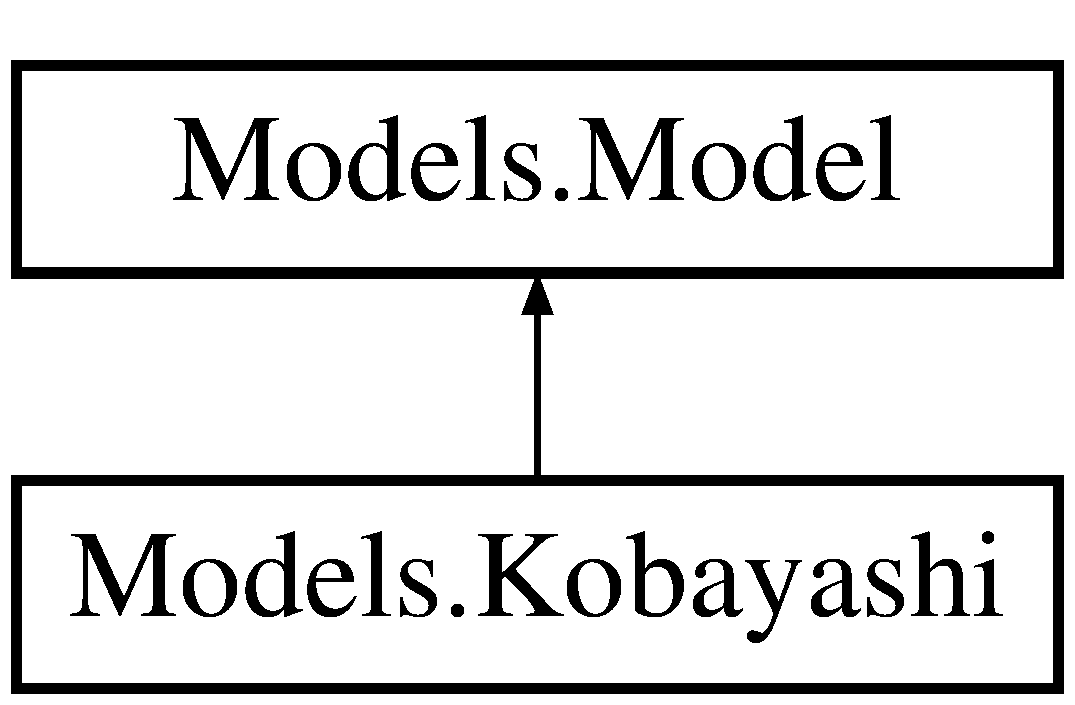
\includegraphics[height=2.000000cm]{classModels_1_1Kobayashi}
\end{center}
\end{figure}
\subsection*{\-Public \-Member \-Functions}
\begin{DoxyCompactItemize}
\item 
\hypertarget{classModels_1_1Kobayashi_ac5360239eb2f57653f4312515b6203ab}{def {\bfseries \-\_\-\-\_\-init\-\_\-\-\_\-}}\label{classModels_1_1Kobayashi_ac5360239eb2f57653f4312515b6203ab}

\item 
def \hyperlink{classModels_1_1Kobayashi_a67ae94b0a84fd06fae51ae5529c6da74}{calc\-Mass}
\item 
def \hyperlink{classModels_1_1Model_a317ed848b969dbe3a96dd05e8b771900}{plt\-Yield}
\item 
def \hyperlink{classModels_1_1Model_aa35c741babf8f141df48c4021e0664e4}{plt\-Rate}
\item 
def \hyperlink{classModels_1_1Model_a3396d6ca1a7b7d66e55ada8c3c7a509e}{max\-Length\-Of\-Vectors}
\item 
def \hyperlink{classModels_1_1Model_ae404a691e48bfe4eafcdfdd09f1dae48}{plot}
\item 
def \hyperlink{classModels_1_1Model_a010945ed2adff59a7a5fce36025e7a97}{derive\-C}
\item 
def \hyperlink{classModels_1_1Model_a7c9280e33f9e0d46703cebc131008c65}{calc\-Rate}
\item 
def \hyperlink{classModels_1_1Model_a818f207e2a4bd0e9a3720ca611960e5a}{set\-Param\-Vector}
\item 
def \hyperlink{classModels_1_1Model_a13c76a0fe24d43cdc4d21fbc73fa96fa}{\-Param\-Vector}
\item 
def \hyperlink{classModels_1_1Model_ad3e627980d9e781bf7b2c9ff900ca06b}{\-Error\-Yield}
\item 
def \hyperlink{classModels_1_1Model_a3050eb39341f318d8d88b172f88bd240}{\-Error\-Rate}
\item 
def \hyperlink{classModels_1_1Model_adcb987bccae63a742490ea1e6d5f7a74}{mk\-Simple\-Result\-Files}
\item 
def \hyperlink{classModels_1_1Model_ac28252ae5cd6b5ecd4c5d006a0e6567d}{set\-Dt4\-Intergrate}
\end{DoxyCompactItemize}
\subsection*{\-Public \-Attributes}
\begin{DoxyCompactItemize}
\item 
\hypertarget{classModels_1_1Kobayashi_a91d6db1083722016a734774d0f002d3b}{{\bfseries \-O\-D\-E\-\_\-hmax}}\label{classModels_1_1Kobayashi_a91d6db1083722016a734774d0f002d3b}

\item 
\hypertarget{classModels_1_1Kobayashi_a222f5faeadc9bd6b15628448c66bd83f}{{\bfseries const\-Dt}}\label{classModels_1_1Kobayashi_a222f5faeadc9bd6b15628448c66bd83f}

\item 
\hypertarget{classModels_1_1Kobayashi_abb0307d1d36a3a9fb9545f626d819c60}{{\bfseries fgdvc}}\label{classModels_1_1Kobayashi_abb0307d1d36a3a9fb9545f626d819c60}

\item 
\hypertarget{classModels_1_1Model_a3f71983de5f8b86bec47929213b900ec}{{\bfseries const\-Dt\-Vec}}\label{classModels_1_1Model_a3f71983de5f8b86bec47929213b900ec}

\end{DoxyCompactItemize}


\subsection{\-Detailed \-Description}
\begin{DoxyVerb}Calculates the devolatilization reaction using the Kobayashi model. The Arrhenius equation inside are in the standard notation.\end{DoxyVerb}
 

\subsection{\-Member \-Function \-Documentation}
\hypertarget{classModels_1_1Kobayashi_a67ae94b0a84fd06fae51ae5529c6da74}{\index{\-Models\-::\-Kobayashi@{\-Models\-::\-Kobayashi}!calc\-Mass@{calc\-Mass}}
\index{calc\-Mass@{calc\-Mass}!Models::Kobayashi@{\-Models\-::\-Kobayashi}}
\subsubsection[{calc\-Mass}]{\setlength{\rightskip}{0pt plus 5cm}def {\bf \-Models.\-Kobayashi.\-calc\-Mass} (
\begin{DoxyParamCaption}
\item[{}]{self, }
\item[{}]{fgdvc, }
\item[{}]{time, }
\item[{}]{\-T, }
\item[{}]{\-Name}
\end{DoxyParamCaption}
)}}\label{classModels_1_1Kobayashi_a67ae94b0a84fd06fae51ae5529c6da74}
\begin{DoxyVerb}Outputs the mass(t) using the model specific equation. The input Vector is [A1,E1,A2,E2,alpha1,alpha2]\end{DoxyVerb}
 \hypertarget{classModels_1_1Model_a7c9280e33f9e0d46703cebc131008c65}{\index{\-Models\-::\-Kobayashi@{\-Models\-::\-Kobayashi}!calc\-Rate@{calc\-Rate}}
\index{calc\-Rate@{calc\-Rate}!Models::Kobayashi@{\-Models\-::\-Kobayashi}}
\subsubsection[{calc\-Rate}]{\setlength{\rightskip}{0pt plus 5cm}def {\bf \-Models.\-Model.\-calc\-Rate} (
\begin{DoxyParamCaption}
\item[{}]{self, }
\item[{}]{fgdvc, }
\item[{}]{time, }
\item[{}]{\-T, }
\item[{}]{\-Name}
\end{DoxyParamCaption}
)\hspace{0.3cm}{\ttfamily  \mbox{[}inherited\mbox{]}}}}\label{classModels_1_1Model_a7c9280e33f9e0d46703cebc131008c65}
\begin{DoxyVerb}Generates the Rates using the yields vector and a CDS.\end{DoxyVerb}
 \hypertarget{classModels_1_1Model_a010945ed2adff59a7a5fce36025e7a97}{\index{\-Models\-::\-Kobayashi@{\-Models\-::\-Kobayashi}!derive\-C@{derive\-C}}
\index{derive\-C@{derive\-C}!Models::Kobayashi@{\-Models\-::\-Kobayashi}}
\subsubsection[{derive\-C}]{\setlength{\rightskip}{0pt plus 5cm}def {\bf \-Models.\-Model.\-derive\-C} (
\begin{DoxyParamCaption}
\item[{}]{self, }
\item[{}]{fgdvc, }
\item[{}]{y\-Vector}
\end{DoxyParamCaption}
)\hspace{0.3cm}{\ttfamily  \mbox{[}inherited\mbox{]}}}}\label{classModels_1_1Model_a010945ed2adff59a7a5fce36025e7a97}
\begin{DoxyVerb}Returns a CDS of the inputted yVector.\end{DoxyVerb}
 \hypertarget{classModels_1_1Model_a3050eb39341f318d8d88b172f88bd240}{\index{\-Models\-::\-Kobayashi@{\-Models\-::\-Kobayashi}!\-Error\-Rate@{\-Error\-Rate}}
\index{\-Error\-Rate@{\-Error\-Rate}!Models::Kobayashi@{\-Models\-::\-Kobayashi}}
\subsubsection[{\-Error\-Rate}]{\setlength{\rightskip}{0pt plus 5cm}def {\bf \-Models.\-Model.\-Error\-Rate} (
\begin{DoxyParamCaption}
\item[{}]{self, }
\item[{}]{fgdvc, }
\item[{}]{\-Species}
\end{DoxyParamCaption}
)\hspace{0.3cm}{\ttfamily  \mbox{[}inherited\mbox{]}}}}\label{classModels_1_1Model_a3050eb39341f318d8d88b172f88bd240}
\begin{DoxyVerb}Returns the absolute deviation per point between the fitted and the original rate curve.\end{DoxyVerb}
 \hypertarget{classModels_1_1Model_ad3e627980d9e781bf7b2c9ff900ca06b}{\index{\-Models\-::\-Kobayashi@{\-Models\-::\-Kobayashi}!\-Error\-Yield@{\-Error\-Yield}}
\index{\-Error\-Yield@{\-Error\-Yield}!Models::Kobayashi@{\-Models\-::\-Kobayashi}}
\subsubsection[{\-Error\-Yield}]{\setlength{\rightskip}{0pt plus 5cm}def {\bf \-Models.\-Model.\-Error\-Yield} (
\begin{DoxyParamCaption}
\item[{}]{self, }
\item[{}]{fgdvc, }
\item[{}]{\-Species}
\end{DoxyParamCaption}
)\hspace{0.3cm}{\ttfamily  \mbox{[}inherited\mbox{]}}}}\label{classModels_1_1Model_ad3e627980d9e781bf7b2c9ff900ca06b}
\begin{DoxyVerb}Returns the absolute deviation per point between the fitted and the original yield curve.\end{DoxyVerb}
 \hypertarget{classModels_1_1Model_a3396d6ca1a7b7d66e55ada8c3c7a509e}{\index{\-Models\-::\-Kobayashi@{\-Models\-::\-Kobayashi}!max\-Length\-Of\-Vectors@{max\-Length\-Of\-Vectors}}
\index{max\-Length\-Of\-Vectors@{max\-Length\-Of\-Vectors}!Models::Kobayashi@{\-Models\-::\-Kobayashi}}
\subsubsection[{max\-Length\-Of\-Vectors}]{\setlength{\rightskip}{0pt plus 5cm}def {\bf \-Models.\-Model.\-max\-Length\-Of\-Vectors} (
\begin{DoxyParamCaption}
\item[{}]{self, }
\item[{}]{fgdvc\-\_\-list}
\end{DoxyParamCaption}
)\hspace{0.3cm}{\ttfamily  \mbox{[}inherited\mbox{]}}}}\label{classModels_1_1Model_a3396d6ca1a7b7d66e55ada8c3c7a509e}
\begin{DoxyVerb}Returns the minimum lenght of a all vectors from the several runs.\end{DoxyVerb}
 \hypertarget{classModels_1_1Model_adcb987bccae63a742490ea1e6d5f7a74}{\index{\-Models\-::\-Kobayashi@{\-Models\-::\-Kobayashi}!mk\-Simple\-Result\-Files@{mk\-Simple\-Result\-Files}}
\index{mk\-Simple\-Result\-Files@{mk\-Simple\-Result\-Files}!Models::Kobayashi@{\-Models\-::\-Kobayashi}}
\subsubsection[{mk\-Simple\-Result\-Files}]{\setlength{\rightskip}{0pt plus 5cm}def {\bf \-Models.\-Model.\-mk\-Simple\-Result\-Files} (
\begin{DoxyParamCaption}
\item[{}]{self, }
\item[{}]{fgdvc\-\_\-list, }
\item[{}]{\-Species}
\end{DoxyParamCaption}
)\hspace{0.3cm}{\ttfamily  \mbox{[}inherited\mbox{]}}}}\label{classModels_1_1Model_adcb987bccae63a742490ea1e6d5f7a74}
\begin{DoxyVerb}Simple result file if no fitting is carried out. Writes only the transformed results into a file.\end{DoxyVerb}
 \hypertarget{classModels_1_1Model_a13c76a0fe24d43cdc4d21fbc73fa96fa}{\index{\-Models\-::\-Kobayashi@{\-Models\-::\-Kobayashi}!\-Param\-Vector@{\-Param\-Vector}}
\index{\-Param\-Vector@{\-Param\-Vector}!Models::Kobayashi@{\-Models\-::\-Kobayashi}}
\subsubsection[{\-Param\-Vector}]{\setlength{\rightskip}{0pt plus 5cm}def {\bf \-Models.\-Model.\-Param\-Vector} (
\begin{DoxyParamCaption}
\item[{}]{self}
\end{DoxyParamCaption}
)\hspace{0.3cm}{\ttfamily  \mbox{[}inherited\mbox{]}}}}\label{classModels_1_1Model_a13c76a0fe24d43cdc4d21fbc73fa96fa}
\begin{DoxyVerb}Returns the Vector containing the kinetic parameter of the Model (refering to the child model).\end{DoxyVerb}
 \hypertarget{classModels_1_1Model_ae404a691e48bfe4eafcdfdd09f1dae48}{\index{\-Models\-::\-Kobayashi@{\-Models\-::\-Kobayashi}!plot@{plot}}
\index{plot@{plot}!Models::Kobayashi@{\-Models\-::\-Kobayashi}}
\subsubsection[{plot}]{\setlength{\rightskip}{0pt plus 5cm}def {\bf \-Models.\-Model.\-plot} (
\begin{DoxyParamCaption}
\item[{}]{self, }
\item[{}]{fgdvc\-\_\-list, }
\item[{}]{\-Species}
\end{DoxyParamCaption}
)\hspace{0.3cm}{\ttfamily  \mbox{[}inherited\mbox{]}}}}\label{classModels_1_1Model_ae404a691e48bfe4eafcdfdd09f1dae48}
\begin{DoxyVerb}Plot the yield and the rates over time with two curves: one is the original data, the other the fitting curve. Also file 'PyrolysisProgramName-Species.out' (e.g. 'CPD-CO2.out') containing the time (s), yields (kg/kg), rates (kg/(kg s)).\end{DoxyVerb}
 \hypertarget{classModels_1_1Model_aa35c741babf8f141df48c4021e0664e4}{\index{\-Models\-::\-Kobayashi@{\-Models\-::\-Kobayashi}!plt\-Rate@{plt\-Rate}}
\index{plt\-Rate@{plt\-Rate}!Models::Kobayashi@{\-Models\-::\-Kobayashi}}
\subsubsection[{plt\-Rate}]{\setlength{\rightskip}{0pt plus 5cm}def {\bf \-Models.\-Model.\-plt\-Rate} (
\begin{DoxyParamCaption}
\item[{}]{self, }
\item[{}]{fgdvc\-\_\-list, }
\item[{}]{x\-Value\-To\-Plot, }
\item[{}]{y\-Value\-To\-Plot}
\end{DoxyParamCaption}
)\hspace{0.3cm}{\ttfamily  \mbox{[}inherited\mbox{]}}}}\label{classModels_1_1Model_aa35c741babf8f141df48c4021e0664e4}
\begin{DoxyVerb}Plots the rates (to select with yValueToPlot) over Time or Temperature (to slect with xValueToPlot).\end{DoxyVerb}
 \hypertarget{classModels_1_1Model_a317ed848b969dbe3a96dd05e8b771900}{\index{\-Models\-::\-Kobayashi@{\-Models\-::\-Kobayashi}!plt\-Yield@{plt\-Yield}}
\index{plt\-Yield@{plt\-Yield}!Models::Kobayashi@{\-Models\-::\-Kobayashi}}
\subsubsection[{plt\-Yield}]{\setlength{\rightskip}{0pt plus 5cm}def {\bf \-Models.\-Model.\-plt\-Yield} (
\begin{DoxyParamCaption}
\item[{}]{self, }
\item[{}]{fgdvc\-\_\-list, }
\item[{}]{x\-Value\-To\-Plot, }
\item[{}]{y\-Value\-To\-Plot}
\end{DoxyParamCaption}
)\hspace{0.3cm}{\ttfamily  \mbox{[}inherited\mbox{]}}}}\label{classModels_1_1Model_a317ed848b969dbe3a96dd05e8b771900}
\begin{DoxyVerb}Plots the yields (to select with yValueToPlot) over Time or Temperature (to slect with xValueToPlot).\end{DoxyVerb}
 \hypertarget{classModels_1_1Model_ac28252ae5cd6b5ecd4c5d006a0e6567d}{\index{\-Models\-::\-Kobayashi@{\-Models\-::\-Kobayashi}!set\-Dt4\-Intergrate@{set\-Dt4\-Intergrate}}
\index{set\-Dt4\-Intergrate@{set\-Dt4\-Intergrate}!Models::Kobayashi@{\-Models\-::\-Kobayashi}}
\subsubsection[{set\-Dt4\-Intergrate}]{\setlength{\rightskip}{0pt plus 5cm}def {\bf \-Models.\-Model.\-set\-Dt4\-Intergrate} (
\begin{DoxyParamCaption}
\item[{}]{self, }
\item[{}]{constant\-Dt}
\end{DoxyParamCaption}
)\hspace{0.3cm}{\ttfamily  \mbox{[}inherited\mbox{]}}}}\label{classModels_1_1Model_ac28252ae5cd6b5ecd4c5d006a0e6567d}
\begin{DoxyVerb}constantDt allows the option to define numerical time step to solve the ODE. The outputted results ever equal the imported time list (when applying method calcMass Time = [t0,t1,t2,t3,t4]. If these time steps are too large, then is this defined dt used to solve the ODE and the results are linear interploated that way that they correspond to the imported time vector. To reset it, just set constantDt to False.\end{DoxyVerb}
 \hypertarget{classModels_1_1Model_a818f207e2a4bd0e9a3720ca611960e5a}{\index{\-Models\-::\-Kobayashi@{\-Models\-::\-Kobayashi}!set\-Param\-Vector@{set\-Param\-Vector}}
\index{set\-Param\-Vector@{set\-Param\-Vector}!Models::Kobayashi@{\-Models\-::\-Kobayashi}}
\subsubsection[{set\-Param\-Vector}]{\setlength{\rightskip}{0pt plus 5cm}def {\bf \-Models.\-Model.\-set\-Param\-Vector} (
\begin{DoxyParamCaption}
\item[{}]{self, }
\item[{}]{\-Parameter\-List}
\end{DoxyParamCaption}
)\hspace{0.3cm}{\ttfamily  \mbox{[}inherited\mbox{]}}}}\label{classModels_1_1Model_a818f207e2a4bd0e9a3720ca611960e5a}
\begin{DoxyVerb}Sets the Vector containing the kinetic parameter of the Model (refering to the child model).\end{DoxyVerb}
 

\-The documentation for this class was generated from the following file\-:\begin{DoxyCompactItemize}
\item 
/home/map/git/pkp/src/\-Models.\-py\end{DoxyCompactItemize}

\hypertarget{classFit__one__run_1_1Kobayashi}{\section{\-Fit\-\_\-one\-\_\-run.\-Kobayashi \-Class \-Reference}
\label{classFit__one__run_1_1Kobayashi}\index{\-Fit\-\_\-one\-\_\-run.\-Kobayashi@{\-Fit\-\_\-one\-\_\-run.\-Kobayashi}}
}
\-Inheritance diagram for \-Fit\-\_\-one\-\_\-run.\-Kobayashi\-:\begin{figure}[H]
\begin{center}
\leavevmode
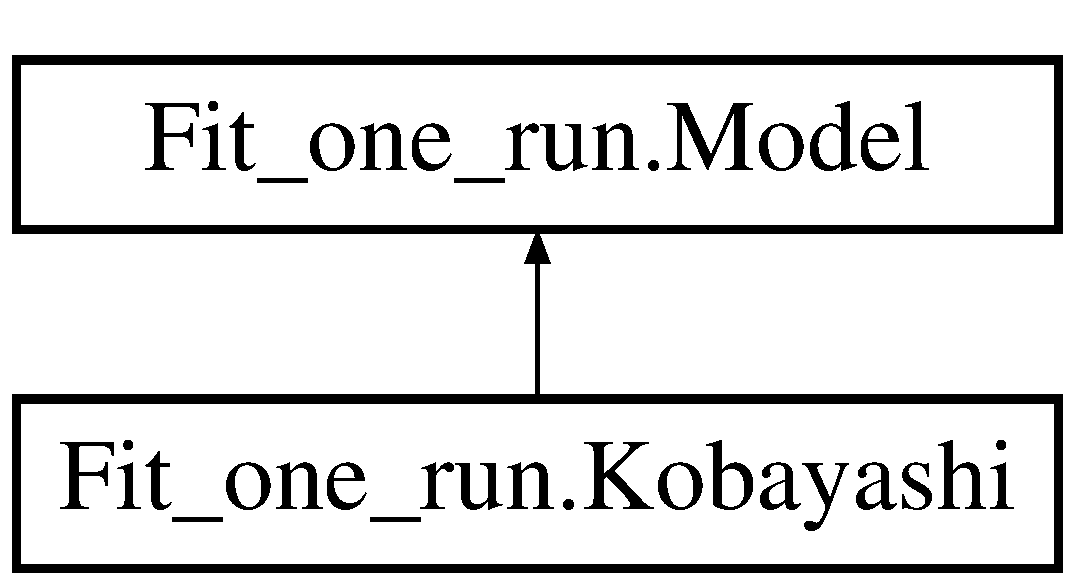
\includegraphics[height=2.000000cm]{classFit__one__run_1_1Kobayashi}
\end{center}
\end{figure}
\subsection*{\-Public \-Member \-Functions}
\begin{DoxyCompactItemize}
\item 
\hypertarget{classFit__one__run_1_1Kobayashi_a14ff386fca6ed35285607b5a8d5724c0}{def {\bfseries \-\_\-\-\_\-init\-\_\-\-\_\-}}\label{classFit__one__run_1_1Kobayashi_a14ff386fca6ed35285607b5a8d5724c0}

\item 
def \hyperlink{classFit__one__run_1_1Kobayashi_a677867f15bf6bb70605b88b7e8607a43}{calc\-Mass}
\item 
def \hyperlink{classFit__one__run_1_1Kobayashi_a3ac4ca157fc46013544cb6ed2db71b3b}{\-Convert\-Kin\-Factors}
\item 
def \hyperlink{classFit__one__run_1_1Kobayashi_a2530abc97e0199bc54d188064c963e78}{set\-Kob\-Weights}
\item 
def \hyperlink{classFit__one__run_1_1Kobayashi_ae381071f0fb8e9c239923a711d338eca}{\-Kob\-Weights}
\item 
def \hyperlink{classFit__one__run_1_1Model_aa304b32155938a713c33f0dc03a135f3}{plt\-Yield}
\item 
def \hyperlink{classFit__one__run_1_1Model_a9c28d95902adf00f5aaa642f0919fc61}{plt\-Rate}
\item 
def \hyperlink{classFit__one__run_1_1Model_a26fc879ca33c9171ebb4a97bc4b0c46b}{min\-Length\-Of\-Vectors}
\item 
def \hyperlink{classFit__one__run_1_1Model_a98159c954f1f1be2a34be3ea53d11493}{plot}
\item 
def \hyperlink{classFit__one__run_1_1Model_ace9df4177c5ae753dbe190e2f8268149}{derive\-C}
\item 
def \hyperlink{classFit__one__run_1_1Model_a07ae4534de2a6ef241d71facdffb227e}{calc\-Rate}
\item 
def \hyperlink{classFit__one__run_1_1Model_a174aec9b05dbe01ec103f7ba75d6516c}{set\-Param\-Vector}
\item 
def \hyperlink{classFit__one__run_1_1Model_a3c9239f0ac062fdae0bda395636c0372}{\-Param\-Vector}
\item 
def \hyperlink{classFit__one__run_1_1Model_aa2bc4ba19704350fb2ff441734b51b10}{\-Error\-Yield}
\item 
def \hyperlink{classFit__one__run_1_1Model_aad63c345c343f0c7d1cf20135dc0a0e5}{\-Error\-Rate}
\end{DoxyCompactItemize}
\subsection*{\-Public \-Attributes}
\begin{DoxyCompactItemize}
\item 
\hypertarget{classFit__one__run_1_1Kobayashi_af2b1dabc461a6f40928ae01a65c448b9}{{\bfseries \-O\-D\-E\-\_\-hmax}}\label{classFit__one__run_1_1Kobayashi_af2b1dabc461a6f40928ae01a65c448b9}

\item 
\hypertarget{classFit__one__run_1_1Kobayashi_abd715c8f6aca9bbaf6e4b56f44f5739a}{{\bfseries fgdvc}}\label{classFit__one__run_1_1Kobayashi_abd715c8f6aca9bbaf6e4b56f44f5739a}

\end{DoxyCompactItemize}


\subsection{\-Detailed \-Description}
\begin{DoxyVerb}Calculates the devolatilization reaction using the Kobayashi model. The Arrhenius equation inside are in the standard notation.\end{DoxyVerb}
 

\subsection{\-Member \-Function \-Documentation}
\hypertarget{classFit__one__run_1_1Kobayashi_a677867f15bf6bb70605b88b7e8607a43}{\index{\-Fit\-\_\-one\-\_\-run\-::\-Kobayashi@{\-Fit\-\_\-one\-\_\-run\-::\-Kobayashi}!calc\-Mass@{calc\-Mass}}
\index{calc\-Mass@{calc\-Mass}!Fit_one_run::Kobayashi@{\-Fit\-\_\-one\-\_\-run\-::\-Kobayashi}}
\subsubsection[{calc\-Mass}]{\setlength{\rightskip}{0pt plus 5cm}def {\bf \-Fit\-\_\-one\-\_\-run.\-Kobayashi.\-calc\-Mass} (
\begin{DoxyParamCaption}
\item[{}]{self, }
\item[{}]{fgdvc, }
\item[{}]{time, }
\item[{}]{\-T, }
\item[{}]{\-Name}
\end{DoxyParamCaption}
)}}\label{classFit__one__run_1_1Kobayashi_a677867f15bf6bb70605b88b7e8607a43}
\begin{DoxyVerb}Outputs the mass(t) using the model specific equation.\end{DoxyVerb}
 \hypertarget{classFit__one__run_1_1Model_a07ae4534de2a6ef241d71facdffb227e}{\index{\-Fit\-\_\-one\-\_\-run\-::\-Kobayashi@{\-Fit\-\_\-one\-\_\-run\-::\-Kobayashi}!calc\-Rate@{calc\-Rate}}
\index{calc\-Rate@{calc\-Rate}!Fit_one_run::Kobayashi@{\-Fit\-\_\-one\-\_\-run\-::\-Kobayashi}}
\subsubsection[{calc\-Rate}]{\setlength{\rightskip}{0pt plus 5cm}def {\bf \-Fit\-\_\-one\-\_\-run.\-Model.\-calc\-Rate} (
\begin{DoxyParamCaption}
\item[{}]{self, }
\item[{}]{fgdvc, }
\item[{}]{time, }
\item[{}]{\-T, }
\item[{}]{\-Name}
\end{DoxyParamCaption}
)\hspace{0.3cm}{\ttfamily  \mbox{[}inherited\mbox{]}}}}\label{classFit__one__run_1_1Model_a07ae4534de2a6ef241d71facdffb227e}
\begin{DoxyVerb}Generates the Rates using the yields vector and a CDS.\end{DoxyVerb}
 \hypertarget{classFit__one__run_1_1Kobayashi_a3ac4ca157fc46013544cb6ed2db71b3b}{\index{\-Fit\-\_\-one\-\_\-run\-::\-Kobayashi@{\-Fit\-\_\-one\-\_\-run\-::\-Kobayashi}!\-Convert\-Kin\-Factors@{\-Convert\-Kin\-Factors}}
\index{\-Convert\-Kin\-Factors@{\-Convert\-Kin\-Factors}!Fit_one_run::Kobayashi@{\-Fit\-\_\-one\-\_\-run\-::\-Kobayashi}}
\subsubsection[{\-Convert\-Kin\-Factors}]{\setlength{\rightskip}{0pt plus 5cm}def {\bf \-Fit\-\_\-one\-\_\-run.\-Kobayashi.\-Convert\-Kin\-Factors} (
\begin{DoxyParamCaption}
\item[{}]{self, }
\item[{}]{\-Parameter\-Vector}
\end{DoxyParamCaption}
)}}\label{classFit__one__run_1_1Kobayashi_a3ac4ca157fc46013544cb6ed2db71b3b}
\begin{DoxyVerb}Outputs the Arrhenius equation factors in the shape [A1,E1,A2,E2,alpha1,alpha2]. Here where the real Arrhenius model is in use only a dummy function.\end{DoxyVerb}
 \hypertarget{classFit__one__run_1_1Model_ace9df4177c5ae753dbe190e2f8268149}{\index{\-Fit\-\_\-one\-\_\-run\-::\-Kobayashi@{\-Fit\-\_\-one\-\_\-run\-::\-Kobayashi}!derive\-C@{derive\-C}}
\index{derive\-C@{derive\-C}!Fit_one_run::Kobayashi@{\-Fit\-\_\-one\-\_\-run\-::\-Kobayashi}}
\subsubsection[{derive\-C}]{\setlength{\rightskip}{0pt plus 5cm}def {\bf \-Fit\-\_\-one\-\_\-run.\-Model.\-derive\-C} (
\begin{DoxyParamCaption}
\item[{}]{self, }
\item[{}]{fgdvc, }
\item[{}]{y\-Vector, }
\item[{}]{max\-Vector\-Lenght = {\ttfamily \-None}}
\end{DoxyParamCaption}
)\hspace{0.3cm}{\ttfamily  \mbox{[}inherited\mbox{]}}}}\label{classFit__one__run_1_1Model_ace9df4177c5ae753dbe190e2f8268149}
\begin{DoxyVerb}Returns a CDS of the inputted yVector.\end{DoxyVerb}
 \hypertarget{classFit__one__run_1_1Model_aad63c345c343f0c7d1cf20135dc0a0e5}{\index{\-Fit\-\_\-one\-\_\-run\-::\-Kobayashi@{\-Fit\-\_\-one\-\_\-run\-::\-Kobayashi}!\-Error\-Rate@{\-Error\-Rate}}
\index{\-Error\-Rate@{\-Error\-Rate}!Fit_one_run::Kobayashi@{\-Fit\-\_\-one\-\_\-run\-::\-Kobayashi}}
\subsubsection[{\-Error\-Rate}]{\setlength{\rightskip}{0pt plus 5cm}def {\bf \-Fit\-\_\-one\-\_\-run.\-Model.\-Error\-Rate} (
\begin{DoxyParamCaption}
\item[{}]{self, }
\item[{}]{fgdvc, }
\item[{}]{\-Species}
\end{DoxyParamCaption}
)\hspace{0.3cm}{\ttfamily  \mbox{[}inherited\mbox{]}}}}\label{classFit__one__run_1_1Model_aad63c345c343f0c7d1cf20135dc0a0e5}
\begin{DoxyVerb}Returns the absolute deviation per point between the fitted and the original rate curve.\end{DoxyVerb}
 \hypertarget{classFit__one__run_1_1Model_aa2bc4ba19704350fb2ff441734b51b10}{\index{\-Fit\-\_\-one\-\_\-run\-::\-Kobayashi@{\-Fit\-\_\-one\-\_\-run\-::\-Kobayashi}!\-Error\-Yield@{\-Error\-Yield}}
\index{\-Error\-Yield@{\-Error\-Yield}!Fit_one_run::Kobayashi@{\-Fit\-\_\-one\-\_\-run\-::\-Kobayashi}}
\subsubsection[{\-Error\-Yield}]{\setlength{\rightskip}{0pt plus 5cm}def {\bf \-Fit\-\_\-one\-\_\-run.\-Model.\-Error\-Yield} (
\begin{DoxyParamCaption}
\item[{}]{self, }
\item[{}]{fgdvc, }
\item[{}]{\-Species}
\end{DoxyParamCaption}
)\hspace{0.3cm}{\ttfamily  \mbox{[}inherited\mbox{]}}}}\label{classFit__one__run_1_1Model_aa2bc4ba19704350fb2ff441734b51b10}
\begin{DoxyVerb}Returns the absolute deviation per point between the fitted and the original yield curve.\end{DoxyVerb}
 \hypertarget{classFit__one__run_1_1Kobayashi_ae381071f0fb8e9c239923a711d338eca}{\index{\-Fit\-\_\-one\-\_\-run\-::\-Kobayashi@{\-Fit\-\_\-one\-\_\-run\-::\-Kobayashi}!\-Kob\-Weights@{\-Kob\-Weights}}
\index{\-Kob\-Weights@{\-Kob\-Weights}!Fit_one_run::Kobayashi@{\-Fit\-\_\-one\-\_\-run\-::\-Kobayashi}}
\subsubsection[{\-Kob\-Weights}]{\setlength{\rightskip}{0pt plus 5cm}def {\bf \-Fit\-\_\-one\-\_\-run.\-Kobayashi.\-Kob\-Weights} (
\begin{DoxyParamCaption}
\item[{}]{self}
\end{DoxyParamCaption}
)}}\label{classFit__one__run_1_1Kobayashi_ae381071f0fb8e9c239923a711d338eca}
\begin{DoxyVerb}Returns the two Kobayashi weights alpha1 and alpha2.\end{DoxyVerb}
 \hypertarget{classFit__one__run_1_1Model_a26fc879ca33c9171ebb4a97bc4b0c46b}{\index{\-Fit\-\_\-one\-\_\-run\-::\-Kobayashi@{\-Fit\-\_\-one\-\_\-run\-::\-Kobayashi}!min\-Length\-Of\-Vectors@{min\-Length\-Of\-Vectors}}
\index{min\-Length\-Of\-Vectors@{min\-Length\-Of\-Vectors}!Fit_one_run::Kobayashi@{\-Fit\-\_\-one\-\_\-run\-::\-Kobayashi}}
\subsubsection[{min\-Length\-Of\-Vectors}]{\setlength{\rightskip}{0pt plus 5cm}def {\bf \-Fit\-\_\-one\-\_\-run.\-Model.\-min\-Length\-Of\-Vectors} (
\begin{DoxyParamCaption}
\item[{}]{self, }
\item[{}]{fgdvc\-\_\-list}
\end{DoxyParamCaption}
)\hspace{0.3cm}{\ttfamily  \mbox{[}inherited\mbox{]}}}}\label{classFit__one__run_1_1Model_a26fc879ca33c9171ebb4a97bc4b0c46b}
\begin{DoxyVerb}Returns the minimum lenght of a all vectors from the several runs.\end{DoxyVerb}
 \hypertarget{classFit__one__run_1_1Model_a3c9239f0ac062fdae0bda395636c0372}{\index{\-Fit\-\_\-one\-\_\-run\-::\-Kobayashi@{\-Fit\-\_\-one\-\_\-run\-::\-Kobayashi}!\-Param\-Vector@{\-Param\-Vector}}
\index{\-Param\-Vector@{\-Param\-Vector}!Fit_one_run::Kobayashi@{\-Fit\-\_\-one\-\_\-run\-::\-Kobayashi}}
\subsubsection[{\-Param\-Vector}]{\setlength{\rightskip}{0pt plus 5cm}def {\bf \-Fit\-\_\-one\-\_\-run.\-Model.\-Param\-Vector} (
\begin{DoxyParamCaption}
\item[{}]{self}
\end{DoxyParamCaption}
)\hspace{0.3cm}{\ttfamily  \mbox{[}inherited\mbox{]}}}}\label{classFit__one__run_1_1Model_a3c9239f0ac062fdae0bda395636c0372}
\begin{DoxyVerb}Returns the Vector containing the kinetic parameter of the Model (refering to the child model).\end{DoxyVerb}
 \hypertarget{classFit__one__run_1_1Model_a98159c954f1f1be2a34be3ea53d11493}{\index{\-Fit\-\_\-one\-\_\-run\-::\-Kobayashi@{\-Fit\-\_\-one\-\_\-run\-::\-Kobayashi}!plot@{plot}}
\index{plot@{plot}!Fit_one_run::Kobayashi@{\-Fit\-\_\-one\-\_\-run\-::\-Kobayashi}}
\subsubsection[{plot}]{\setlength{\rightskip}{0pt plus 5cm}def {\bf \-Fit\-\_\-one\-\_\-run.\-Model.\-plot} (
\begin{DoxyParamCaption}
\item[{}]{self, }
\item[{}]{fgdvc\-\_\-list, }
\item[{}]{\-Species}
\end{DoxyParamCaption}
)\hspace{0.3cm}{\ttfamily  \mbox{[}inherited\mbox{]}}}}\label{classFit__one__run_1_1Model_a98159c954f1f1be2a34be3ea53d11493}
\begin{DoxyVerb}Plot the yield and the rates over time with two curves: one is the original data, the other the fitting curve. Also file 'PyrolysisProgramName-Species.out' (e.g. 'CPD-CO2.out') containing the time (s), yields (kg/kg), rates (kg/(kg s)).\end{DoxyVerb}
 \hypertarget{classFit__one__run_1_1Model_a9c28d95902adf00f5aaa642f0919fc61}{\index{\-Fit\-\_\-one\-\_\-run\-::\-Kobayashi@{\-Fit\-\_\-one\-\_\-run\-::\-Kobayashi}!plt\-Rate@{plt\-Rate}}
\index{plt\-Rate@{plt\-Rate}!Fit_one_run::Kobayashi@{\-Fit\-\_\-one\-\_\-run\-::\-Kobayashi}}
\subsubsection[{plt\-Rate}]{\setlength{\rightskip}{0pt plus 5cm}def {\bf \-Fit\-\_\-one\-\_\-run.\-Model.\-plt\-Rate} (
\begin{DoxyParamCaption}
\item[{}]{self, }
\item[{}]{fgdvc\-\_\-list, }
\item[{}]{x\-Value\-To\-Plot, }
\item[{}]{y\-Value\-To\-Plot}
\end{DoxyParamCaption}
)\hspace{0.3cm}{\ttfamily  \mbox{[}inherited\mbox{]}}}}\label{classFit__one__run_1_1Model_a9c28d95902adf00f5aaa642f0919fc61}
\begin{DoxyVerb}Plots the rates (to select with yValueToPlot) over Time or Temperature (to slect with xValueToPlot).\end{DoxyVerb}
 \hypertarget{classFit__one__run_1_1Model_aa304b32155938a713c33f0dc03a135f3}{\index{\-Fit\-\_\-one\-\_\-run\-::\-Kobayashi@{\-Fit\-\_\-one\-\_\-run\-::\-Kobayashi}!plt\-Yield@{plt\-Yield}}
\index{plt\-Yield@{plt\-Yield}!Fit_one_run::Kobayashi@{\-Fit\-\_\-one\-\_\-run\-::\-Kobayashi}}
\subsubsection[{plt\-Yield}]{\setlength{\rightskip}{0pt plus 5cm}def {\bf \-Fit\-\_\-one\-\_\-run.\-Model.\-plt\-Yield} (
\begin{DoxyParamCaption}
\item[{}]{self, }
\item[{}]{fgdvc\-\_\-list, }
\item[{}]{x\-Value\-To\-Plot, }
\item[{}]{y\-Value\-To\-Plot}
\end{DoxyParamCaption}
)\hspace{0.3cm}{\ttfamily  \mbox{[}inherited\mbox{]}}}}\label{classFit__one__run_1_1Model_aa304b32155938a713c33f0dc03a135f3}
\begin{DoxyVerb}Plots the yields (to select with yValueToPlot) over Time or Temperature (to slect with xValueToPlot).\end{DoxyVerb}
 \hypertarget{classFit__one__run_1_1Kobayashi_a2530abc97e0199bc54d188064c963e78}{\index{\-Fit\-\_\-one\-\_\-run\-::\-Kobayashi@{\-Fit\-\_\-one\-\_\-run\-::\-Kobayashi}!set\-Kob\-Weights@{set\-Kob\-Weights}}
\index{set\-Kob\-Weights@{set\-Kob\-Weights}!Fit_one_run::Kobayashi@{\-Fit\-\_\-one\-\_\-run\-::\-Kobayashi}}
\subsubsection[{set\-Kob\-Weights}]{\setlength{\rightskip}{0pt plus 5cm}def {\bf \-Fit\-\_\-one\-\_\-run.\-Kobayashi.\-set\-Kob\-Weights} (
\begin{DoxyParamCaption}
\item[{}]{self, }
\item[{}]{alpha1, }
\item[{}]{alpha2}
\end{DoxyParamCaption}
)}}\label{classFit__one__run_1_1Kobayashi_a2530abc97e0199bc54d188064c963e78}
\begin{DoxyVerb}Sets the two Kobayashi weights alpha1 and alpha2.\end{DoxyVerb}
 \hypertarget{classFit__one__run_1_1Model_a174aec9b05dbe01ec103f7ba75d6516c}{\index{\-Fit\-\_\-one\-\_\-run\-::\-Kobayashi@{\-Fit\-\_\-one\-\_\-run\-::\-Kobayashi}!set\-Param\-Vector@{set\-Param\-Vector}}
\index{set\-Param\-Vector@{set\-Param\-Vector}!Fit_one_run::Kobayashi@{\-Fit\-\_\-one\-\_\-run\-::\-Kobayashi}}
\subsubsection[{set\-Param\-Vector}]{\setlength{\rightskip}{0pt plus 5cm}def {\bf \-Fit\-\_\-one\-\_\-run.\-Model.\-set\-Param\-Vector} (
\begin{DoxyParamCaption}
\item[{}]{self, }
\item[{}]{\-Parameter\-List}
\end{DoxyParamCaption}
)\hspace{0.3cm}{\ttfamily  \mbox{[}inherited\mbox{]}}}}\label{classFit__one__run_1_1Model_a174aec9b05dbe01ec103f7ba75d6516c}
\begin{DoxyVerb}Sets the Vector containing the kinetic parameter of the Model (refering to the child model).\end{DoxyVerb}
 

\-The documentation for this class was generated from the following file\-:\begin{DoxyCompactItemize}
\item 
/home/map/git/pkp/src/\-Fit\-\_\-one\-\_\-run.\-py\end{DoxyCompactItemize}

\hypertarget{classModels_1_1KobayashiA2}{\section{\-Models.\-Kobayashi\-A2 \-Class \-Reference}
\label{classModels_1_1KobayashiA2}\index{\-Models.\-Kobayashi\-A2@{\-Models.\-Kobayashi\-A2}}
}
\-Inheritance diagram for \-Models.\-Kobayashi\-A2\-:\begin{figure}[H]
\begin{center}
\leavevmode
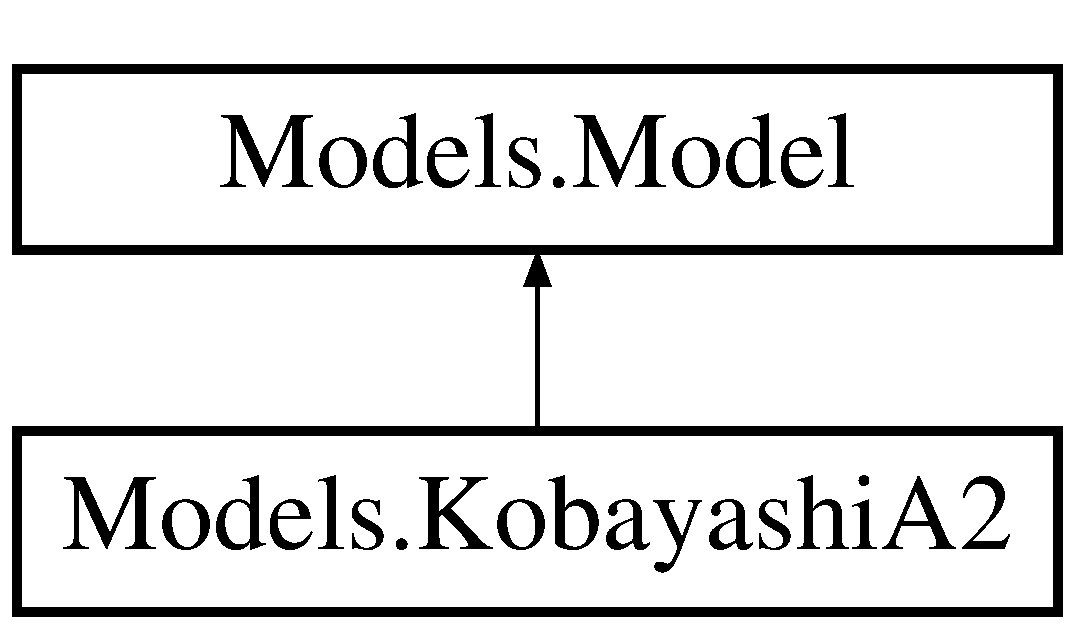
\includegraphics[height=2.000000cm]{classModels_1_1KobayashiA2}
\end{center}
\end{figure}
\subsection*{\-Public \-Member \-Functions}
\begin{DoxyCompactItemize}
\item 
\hypertarget{classModels_1_1KobayashiA2_a5a22e7f37b899751b8611a3f06c988f2}{def {\bfseries \-\_\-\-\_\-init\-\_\-\-\_\-}}\label{classModels_1_1KobayashiA2_a5a22e7f37b899751b8611a3f06c988f2}

\item 
def \hyperlink{classModels_1_1KobayashiA2_a7fc4650e426fa4b341795d9508176ea3}{calc\-Mass}
\item 
def \hyperlink{classModels_1_1KobayashiA2_a29386cb0487ceb6ff432468a20d12c81}{\-Convert\-Kin\-Factors}
\item 
def \hyperlink{classModels_1_1KobayashiA2_ade04a3424cfd823d7cd5e2b99abcbc46}{set\-Kob\-Weights}
\item 
def \hyperlink{classModels_1_1KobayashiA2_aa4302551de83a7fdc46d1e73d1ea4a27}{\-Kob\-Weights}
\item 
def \hyperlink{classModels_1_1Model_a317ed848b969dbe3a96dd05e8b771900}{plt\-Yield}
\item 
def \hyperlink{classModels_1_1Model_aa35c741babf8f141df48c4021e0664e4}{plt\-Rate}
\item 
def \hyperlink{classModels_1_1Model_a3396d6ca1a7b7d66e55ada8c3c7a509e}{max\-Length\-Of\-Vectors}
\item 
def \hyperlink{classModels_1_1Model_ae404a691e48bfe4eafcdfdd09f1dae48}{plot}
\item 
def \hyperlink{classModels_1_1Model_a010945ed2adff59a7a5fce36025e7a97}{derive\-C}
\item 
def \hyperlink{classModels_1_1Model_a7c9280e33f9e0d46703cebc131008c65}{calc\-Rate}
\item 
def \hyperlink{classModels_1_1Model_a818f207e2a4bd0e9a3720ca611960e5a}{set\-Param\-Vector}
\item 
def \hyperlink{classModels_1_1Model_a13c76a0fe24d43cdc4d21fbc73fa96fa}{\-Param\-Vector}
\item 
def \hyperlink{classModels_1_1Model_ad3e627980d9e781bf7b2c9ff900ca06b}{\-Error\-Yield}
\item 
def \hyperlink{classModels_1_1Model_a3050eb39341f318d8d88b172f88bd240}{\-Error\-Rate}
\item 
def \hyperlink{classModels_1_1Model_adcb987bccae63a742490ea1e6d5f7a74}{mk\-Simple\-Result\-Files}
\item 
def \hyperlink{classModels_1_1Model_ac28252ae5cd6b5ecd4c5d006a0e6567d}{set\-Dt4\-Intergrate}
\end{DoxyCompactItemize}
\subsection*{\-Public \-Attributes}
\begin{DoxyCompactItemize}
\item 
\hypertarget{classModels_1_1KobayashiA2_a8f0727a152bc7bd410b0209a8554d05f}{{\bfseries \-O\-D\-E\-\_\-hmax}}\label{classModels_1_1KobayashiA2_a8f0727a152bc7bd410b0209a8554d05f}

\item 
\hypertarget{classModels_1_1KobayashiA2_a0363b5427cff1b05f81ad263cf78f2f0}{{\bfseries const\-Dt}}\label{classModels_1_1KobayashiA2_a0363b5427cff1b05f81ad263cf78f2f0}

\item 
\hypertarget{classModels_1_1KobayashiA2_ac7cd81e12988ff443f46d0ca7b097d73}{{\bfseries fgdvc}}\label{classModels_1_1KobayashiA2_ac7cd81e12988ff443f46d0ca7b097d73}

\item 
\hypertarget{classModels_1_1KobayashiA2_ab341f4b57d9aacd30c84e57e508285c4}{{\bfseries \-T\-\_\-min}}\label{classModels_1_1KobayashiA2_ab341f4b57d9aacd30c84e57e508285c4}

\item 
\hypertarget{classModels_1_1KobayashiA2_adb28410cd1202c1467d44eec1b28b260}{{\bfseries \-T\-\_\-max}}\label{classModels_1_1KobayashiA2_adb28410cd1202c1467d44eec1b28b260}

\item 
\hypertarget{classModels_1_1KobayashiA2_adc730460f18944e9e7f07b5e659cffbc}{{\bfseries c}}\label{classModels_1_1KobayashiA2_adc730460f18944e9e7f07b5e659cffbc}

\item 
\hypertarget{classModels_1_1KobayashiA2_afed741d2c24b16299ffdfb0fd87a0554}{{\bfseries t\-List}}\label{classModels_1_1KobayashiA2_afed741d2c24b16299ffdfb0fd87a0554}

\item 
\hypertarget{classModels_1_1KobayashiA2_a79a7f1db1d7dbb3918664b6f9427195f}{{\bfseries \-Integral}}\label{classModels_1_1KobayashiA2_a79a7f1db1d7dbb3918664b6f9427195f}

\item 
\hypertarget{classModels_1_1KobayashiA2_aaab691238b4a392e91e2239139b1365c}{{\bfseries k1k2}}\label{classModels_1_1KobayashiA2_aaab691238b4a392e91e2239139b1365c}

\item 
\hypertarget{classModels_1_1Model_a3f71983de5f8b86bec47929213b900ec}{{\bfseries const\-Dt\-Vec}}\label{classModels_1_1Model_a3f71983de5f8b86bec47929213b900ec}

\end{DoxyCompactItemize}


\subsection{\-Detailed \-Description}
\begin{DoxyVerb}Calculates the devolatilization reaction using the Kobayashi model. The Arrhenius equation inside are in the secend alternative notation (see class ArrheniusModelAlternativeNotation2).\end{DoxyVerb}
 

\subsection{\-Member \-Function \-Documentation}
\hypertarget{classModels_1_1KobayashiA2_a7fc4650e426fa4b341795d9508176ea3}{\index{\-Models\-::\-Kobayashi\-A2@{\-Models\-::\-Kobayashi\-A2}!calc\-Mass@{calc\-Mass}}
\index{calc\-Mass@{calc\-Mass}!Models::KobayashiA2@{\-Models\-::\-Kobayashi\-A2}}
\subsubsection[{calc\-Mass}]{\setlength{\rightskip}{0pt plus 5cm}def {\bf \-Models.\-Kobayashi\-A2.\-calc\-Mass} (
\begin{DoxyParamCaption}
\item[{}]{self, }
\item[{}]{fgdvc, }
\item[{}]{time, }
\item[{}]{\-T, }
\item[{}]{\-Name}
\end{DoxyParamCaption}
)}}\label{classModels_1_1KobayashiA2_a7fc4650e426fa4b341795d9508176ea3}
\begin{DoxyVerb}Outputs the mass(t) using the model specific equation.\end{DoxyVerb}
 \hypertarget{classModels_1_1Model_a7c9280e33f9e0d46703cebc131008c65}{\index{\-Models\-::\-Kobayashi\-A2@{\-Models\-::\-Kobayashi\-A2}!calc\-Rate@{calc\-Rate}}
\index{calc\-Rate@{calc\-Rate}!Models::KobayashiA2@{\-Models\-::\-Kobayashi\-A2}}
\subsubsection[{calc\-Rate}]{\setlength{\rightskip}{0pt plus 5cm}def {\bf \-Models.\-Model.\-calc\-Rate} (
\begin{DoxyParamCaption}
\item[{}]{self, }
\item[{}]{fgdvc, }
\item[{}]{time, }
\item[{}]{\-T, }
\item[{}]{\-Name}
\end{DoxyParamCaption}
)\hspace{0.3cm}{\ttfamily  \mbox{[}inherited\mbox{]}}}}\label{classModels_1_1Model_a7c9280e33f9e0d46703cebc131008c65}
\begin{DoxyVerb}Generates the Rates using the yields vector and a CDS.\end{DoxyVerb}
 \hypertarget{classModels_1_1KobayashiA2_a29386cb0487ceb6ff432468a20d12c81}{\index{\-Models\-::\-Kobayashi\-A2@{\-Models\-::\-Kobayashi\-A2}!\-Convert\-Kin\-Factors@{\-Convert\-Kin\-Factors}}
\index{\-Convert\-Kin\-Factors@{\-Convert\-Kin\-Factors}!Models::KobayashiA2@{\-Models\-::\-Kobayashi\-A2}}
\subsubsection[{\-Convert\-Kin\-Factors}]{\setlength{\rightskip}{0pt plus 5cm}def {\bf \-Models.\-Kobayashi\-A2.\-Convert\-Kin\-Factors} (
\begin{DoxyParamCaption}
\item[{}]{self, }
\item[{}]{\-Parameter\-Vector}
\end{DoxyParamCaption}
)}}\label{classModels_1_1KobayashiA2_a29386cb0487ceb6ff432468a20d12c81}
\begin{DoxyVerb}Converts the alternative notaion Arrhenius factors into the satndard Arrhenius factors and return them in the shape  [A1,E1], [A2,E2]\end{DoxyVerb}
 \hypertarget{classModels_1_1Model_a010945ed2adff59a7a5fce36025e7a97}{\index{\-Models\-::\-Kobayashi\-A2@{\-Models\-::\-Kobayashi\-A2}!derive\-C@{derive\-C}}
\index{derive\-C@{derive\-C}!Models::KobayashiA2@{\-Models\-::\-Kobayashi\-A2}}
\subsubsection[{derive\-C}]{\setlength{\rightskip}{0pt plus 5cm}def {\bf \-Models.\-Model.\-derive\-C} (
\begin{DoxyParamCaption}
\item[{}]{self, }
\item[{}]{fgdvc, }
\item[{}]{y\-Vector}
\end{DoxyParamCaption}
)\hspace{0.3cm}{\ttfamily  \mbox{[}inherited\mbox{]}}}}\label{classModels_1_1Model_a010945ed2adff59a7a5fce36025e7a97}
\begin{DoxyVerb}Returns a CDS of the inputted yVector.\end{DoxyVerb}
 \hypertarget{classModels_1_1Model_a3050eb39341f318d8d88b172f88bd240}{\index{\-Models\-::\-Kobayashi\-A2@{\-Models\-::\-Kobayashi\-A2}!\-Error\-Rate@{\-Error\-Rate}}
\index{\-Error\-Rate@{\-Error\-Rate}!Models::KobayashiA2@{\-Models\-::\-Kobayashi\-A2}}
\subsubsection[{\-Error\-Rate}]{\setlength{\rightskip}{0pt plus 5cm}def {\bf \-Models.\-Model.\-Error\-Rate} (
\begin{DoxyParamCaption}
\item[{}]{self, }
\item[{}]{fgdvc, }
\item[{}]{\-Species}
\end{DoxyParamCaption}
)\hspace{0.3cm}{\ttfamily  \mbox{[}inherited\mbox{]}}}}\label{classModels_1_1Model_a3050eb39341f318d8d88b172f88bd240}
\begin{DoxyVerb}Returns the absolute deviation per point between the fitted and the original rate curve.\end{DoxyVerb}
 \hypertarget{classModels_1_1Model_ad3e627980d9e781bf7b2c9ff900ca06b}{\index{\-Models\-::\-Kobayashi\-A2@{\-Models\-::\-Kobayashi\-A2}!\-Error\-Yield@{\-Error\-Yield}}
\index{\-Error\-Yield@{\-Error\-Yield}!Models::KobayashiA2@{\-Models\-::\-Kobayashi\-A2}}
\subsubsection[{\-Error\-Yield}]{\setlength{\rightskip}{0pt plus 5cm}def {\bf \-Models.\-Model.\-Error\-Yield} (
\begin{DoxyParamCaption}
\item[{}]{self, }
\item[{}]{fgdvc, }
\item[{}]{\-Species}
\end{DoxyParamCaption}
)\hspace{0.3cm}{\ttfamily  \mbox{[}inherited\mbox{]}}}}\label{classModels_1_1Model_ad3e627980d9e781bf7b2c9ff900ca06b}
\begin{DoxyVerb}Returns the absolute deviation per point between the fitted and the original yield curve.\end{DoxyVerb}
 \hypertarget{classModels_1_1KobayashiA2_aa4302551de83a7fdc46d1e73d1ea4a27}{\index{\-Models\-::\-Kobayashi\-A2@{\-Models\-::\-Kobayashi\-A2}!\-Kob\-Weights@{\-Kob\-Weights}}
\index{\-Kob\-Weights@{\-Kob\-Weights}!Models::KobayashiA2@{\-Models\-::\-Kobayashi\-A2}}
\subsubsection[{\-Kob\-Weights}]{\setlength{\rightskip}{0pt plus 5cm}def {\bf \-Models.\-Kobayashi\-A2.\-Kob\-Weights} (
\begin{DoxyParamCaption}
\item[{}]{self}
\end{DoxyParamCaption}
)}}\label{classModels_1_1KobayashiA2_aa4302551de83a7fdc46d1e73d1ea4a27}
\begin{DoxyVerb}Returns the two Kobayashi weights alpha1 and alpha2.\end{DoxyVerb}
 \hypertarget{classModels_1_1Model_a3396d6ca1a7b7d66e55ada8c3c7a509e}{\index{\-Models\-::\-Kobayashi\-A2@{\-Models\-::\-Kobayashi\-A2}!max\-Length\-Of\-Vectors@{max\-Length\-Of\-Vectors}}
\index{max\-Length\-Of\-Vectors@{max\-Length\-Of\-Vectors}!Models::KobayashiA2@{\-Models\-::\-Kobayashi\-A2}}
\subsubsection[{max\-Length\-Of\-Vectors}]{\setlength{\rightskip}{0pt plus 5cm}def {\bf \-Models.\-Model.\-max\-Length\-Of\-Vectors} (
\begin{DoxyParamCaption}
\item[{}]{self, }
\item[{}]{fgdvc\-\_\-list}
\end{DoxyParamCaption}
)\hspace{0.3cm}{\ttfamily  \mbox{[}inherited\mbox{]}}}}\label{classModels_1_1Model_a3396d6ca1a7b7d66e55ada8c3c7a509e}
\begin{DoxyVerb}Returns the minimum lenght of a all vectors from the several runs.\end{DoxyVerb}
 \hypertarget{classModels_1_1Model_adcb987bccae63a742490ea1e6d5f7a74}{\index{\-Models\-::\-Kobayashi\-A2@{\-Models\-::\-Kobayashi\-A2}!mk\-Simple\-Result\-Files@{mk\-Simple\-Result\-Files}}
\index{mk\-Simple\-Result\-Files@{mk\-Simple\-Result\-Files}!Models::KobayashiA2@{\-Models\-::\-Kobayashi\-A2}}
\subsubsection[{mk\-Simple\-Result\-Files}]{\setlength{\rightskip}{0pt plus 5cm}def {\bf \-Models.\-Model.\-mk\-Simple\-Result\-Files} (
\begin{DoxyParamCaption}
\item[{}]{self, }
\item[{}]{fgdvc\-\_\-list, }
\item[{}]{\-Species}
\end{DoxyParamCaption}
)\hspace{0.3cm}{\ttfamily  \mbox{[}inherited\mbox{]}}}}\label{classModels_1_1Model_adcb987bccae63a742490ea1e6d5f7a74}
\begin{DoxyVerb}Simple result file if no fitting is carried out. Writes only the transformed results into a file.\end{DoxyVerb}
 \hypertarget{classModels_1_1Model_a13c76a0fe24d43cdc4d21fbc73fa96fa}{\index{\-Models\-::\-Kobayashi\-A2@{\-Models\-::\-Kobayashi\-A2}!\-Param\-Vector@{\-Param\-Vector}}
\index{\-Param\-Vector@{\-Param\-Vector}!Models::KobayashiA2@{\-Models\-::\-Kobayashi\-A2}}
\subsubsection[{\-Param\-Vector}]{\setlength{\rightskip}{0pt plus 5cm}def {\bf \-Models.\-Model.\-Param\-Vector} (
\begin{DoxyParamCaption}
\item[{}]{self}
\end{DoxyParamCaption}
)\hspace{0.3cm}{\ttfamily  \mbox{[}inherited\mbox{]}}}}\label{classModels_1_1Model_a13c76a0fe24d43cdc4d21fbc73fa96fa}
\begin{DoxyVerb}Returns the Vector containing the kinetic parameter of the Model (refering to the child model).\end{DoxyVerb}
 \hypertarget{classModels_1_1Model_ae404a691e48bfe4eafcdfdd09f1dae48}{\index{\-Models\-::\-Kobayashi\-A2@{\-Models\-::\-Kobayashi\-A2}!plot@{plot}}
\index{plot@{plot}!Models::KobayashiA2@{\-Models\-::\-Kobayashi\-A2}}
\subsubsection[{plot}]{\setlength{\rightskip}{0pt plus 5cm}def {\bf \-Models.\-Model.\-plot} (
\begin{DoxyParamCaption}
\item[{}]{self, }
\item[{}]{fgdvc\-\_\-list, }
\item[{}]{\-Species}
\end{DoxyParamCaption}
)\hspace{0.3cm}{\ttfamily  \mbox{[}inherited\mbox{]}}}}\label{classModels_1_1Model_ae404a691e48bfe4eafcdfdd09f1dae48}
\begin{DoxyVerb}Plot the yield and the rates over time with two curves: one is the original data, the other the fitting curve. Also file 'PyrolysisProgramName-Species.out' (e.g. 'CPD-CO2.out') containing the time (s), yields (kg/kg), rates (kg/(kg s)).\end{DoxyVerb}
 \hypertarget{classModels_1_1Model_aa35c741babf8f141df48c4021e0664e4}{\index{\-Models\-::\-Kobayashi\-A2@{\-Models\-::\-Kobayashi\-A2}!plt\-Rate@{plt\-Rate}}
\index{plt\-Rate@{plt\-Rate}!Models::KobayashiA2@{\-Models\-::\-Kobayashi\-A2}}
\subsubsection[{plt\-Rate}]{\setlength{\rightskip}{0pt plus 5cm}def {\bf \-Models.\-Model.\-plt\-Rate} (
\begin{DoxyParamCaption}
\item[{}]{self, }
\item[{}]{fgdvc\-\_\-list, }
\item[{}]{x\-Value\-To\-Plot, }
\item[{}]{y\-Value\-To\-Plot}
\end{DoxyParamCaption}
)\hspace{0.3cm}{\ttfamily  \mbox{[}inherited\mbox{]}}}}\label{classModels_1_1Model_aa35c741babf8f141df48c4021e0664e4}
\begin{DoxyVerb}Plots the rates (to select with yValueToPlot) over Time or Temperature (to slect with xValueToPlot).\end{DoxyVerb}
 \hypertarget{classModels_1_1Model_a317ed848b969dbe3a96dd05e8b771900}{\index{\-Models\-::\-Kobayashi\-A2@{\-Models\-::\-Kobayashi\-A2}!plt\-Yield@{plt\-Yield}}
\index{plt\-Yield@{plt\-Yield}!Models::KobayashiA2@{\-Models\-::\-Kobayashi\-A2}}
\subsubsection[{plt\-Yield}]{\setlength{\rightskip}{0pt plus 5cm}def {\bf \-Models.\-Model.\-plt\-Yield} (
\begin{DoxyParamCaption}
\item[{}]{self, }
\item[{}]{fgdvc\-\_\-list, }
\item[{}]{x\-Value\-To\-Plot, }
\item[{}]{y\-Value\-To\-Plot}
\end{DoxyParamCaption}
)\hspace{0.3cm}{\ttfamily  \mbox{[}inherited\mbox{]}}}}\label{classModels_1_1Model_a317ed848b969dbe3a96dd05e8b771900}
\begin{DoxyVerb}Plots the yields (to select with yValueToPlot) over Time or Temperature (to slect with xValueToPlot).\end{DoxyVerb}
 \hypertarget{classModels_1_1Model_ac28252ae5cd6b5ecd4c5d006a0e6567d}{\index{\-Models\-::\-Kobayashi\-A2@{\-Models\-::\-Kobayashi\-A2}!set\-Dt4\-Intergrate@{set\-Dt4\-Intergrate}}
\index{set\-Dt4\-Intergrate@{set\-Dt4\-Intergrate}!Models::KobayashiA2@{\-Models\-::\-Kobayashi\-A2}}
\subsubsection[{set\-Dt4\-Intergrate}]{\setlength{\rightskip}{0pt plus 5cm}def {\bf \-Models.\-Model.\-set\-Dt4\-Intergrate} (
\begin{DoxyParamCaption}
\item[{}]{self, }
\item[{}]{constant\-Dt}
\end{DoxyParamCaption}
)\hspace{0.3cm}{\ttfamily  \mbox{[}inherited\mbox{]}}}}\label{classModels_1_1Model_ac28252ae5cd6b5ecd4c5d006a0e6567d}
\begin{DoxyVerb}constantDt allows the option to define numerical time step to solve the ODE. The outputted results ever equal the imported time list (when applying method calcMass Time = [t0,t1,t2,t3,t4]. If these time steps are too large, then is this defined dt used to solve the ODE and the results are linear interploated that way that they correspond to the imported time vector. To reset it, just set constantDt to False.\end{DoxyVerb}
 \hypertarget{classModels_1_1KobayashiA2_ade04a3424cfd823d7cd5e2b99abcbc46}{\index{\-Models\-::\-Kobayashi\-A2@{\-Models\-::\-Kobayashi\-A2}!set\-Kob\-Weights@{set\-Kob\-Weights}}
\index{set\-Kob\-Weights@{set\-Kob\-Weights}!Models::KobayashiA2@{\-Models\-::\-Kobayashi\-A2}}
\subsubsection[{set\-Kob\-Weights}]{\setlength{\rightskip}{0pt plus 5cm}def {\bf \-Models.\-Kobayashi\-A2.\-set\-Kob\-Weights} (
\begin{DoxyParamCaption}
\item[{}]{self, }
\item[{}]{alpha1, }
\item[{}]{alpha2}
\end{DoxyParamCaption}
)}}\label{classModels_1_1KobayashiA2_ade04a3424cfd823d7cd5e2b99abcbc46}
\begin{DoxyVerb}Sets the two Kobayashi weights alpha1 and alpha2.\end{DoxyVerb}
 \hypertarget{classModels_1_1Model_a818f207e2a4bd0e9a3720ca611960e5a}{\index{\-Models\-::\-Kobayashi\-A2@{\-Models\-::\-Kobayashi\-A2}!set\-Param\-Vector@{set\-Param\-Vector}}
\index{set\-Param\-Vector@{set\-Param\-Vector}!Models::KobayashiA2@{\-Models\-::\-Kobayashi\-A2}}
\subsubsection[{set\-Param\-Vector}]{\setlength{\rightskip}{0pt plus 5cm}def {\bf \-Models.\-Model.\-set\-Param\-Vector} (
\begin{DoxyParamCaption}
\item[{}]{self, }
\item[{}]{\-Parameter\-List}
\end{DoxyParamCaption}
)\hspace{0.3cm}{\ttfamily  \mbox{[}inherited\mbox{]}}}}\label{classModels_1_1Model_a818f207e2a4bd0e9a3720ca611960e5a}
\begin{DoxyVerb}Sets the Vector containing the kinetic parameter of the Model (refering to the child model).\end{DoxyVerb}
 

\-The documentation for this class was generated from the following file\-:\begin{DoxyCompactItemize}
\item 
/home/map/git/pkp/src/\-Models.\-py\end{DoxyCompactItemize}

\hypertarget{classFit__one__run_1_1KobayashiA2}{\section{\-Fit\-\_\-one\-\_\-run.\-Kobayashi\-A2 \-Class \-Reference}
\label{classFit__one__run_1_1KobayashiA2}\index{\-Fit\-\_\-one\-\_\-run.\-Kobayashi\-A2@{\-Fit\-\_\-one\-\_\-run.\-Kobayashi\-A2}}
}
\-Inheritance diagram for \-Fit\-\_\-one\-\_\-run.\-Kobayashi\-A2\-:\begin{figure}[H]
\begin{center}
\leavevmode
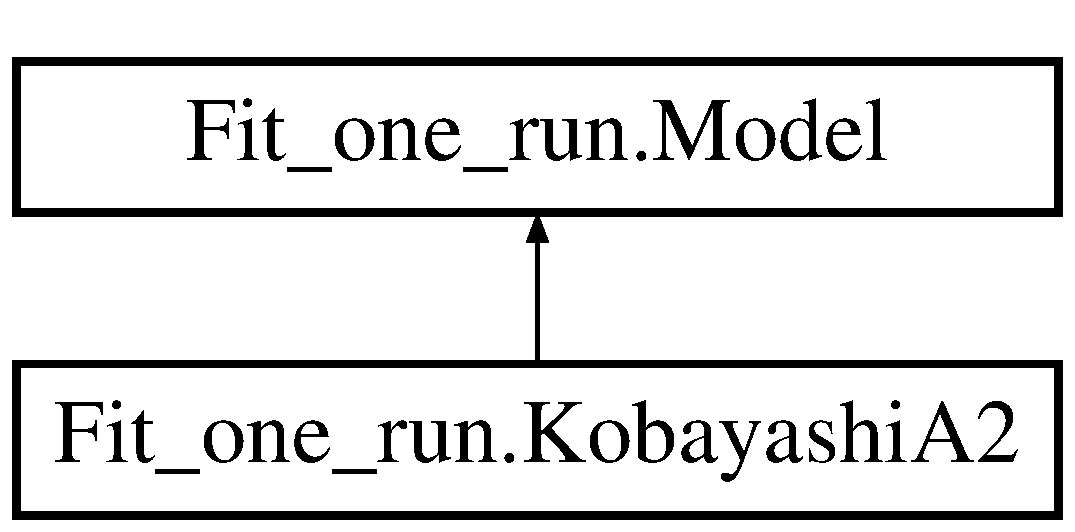
\includegraphics[height=2.000000cm]{classFit__one__run_1_1KobayashiA2}
\end{center}
\end{figure}
\subsection*{\-Public \-Member \-Functions}
\begin{DoxyCompactItemize}
\item 
\hypertarget{classFit__one__run_1_1KobayashiA2_a7eea093af89e02cb275ea803f1444289}{def {\bfseries \-\_\-\-\_\-init\-\_\-\-\_\-}}\label{classFit__one__run_1_1KobayashiA2_a7eea093af89e02cb275ea803f1444289}

\item 
def \hyperlink{classFit__one__run_1_1KobayashiA2_a9b6b0c05b852f733c38af2cbf9bc06cf}{calc\-Mass}
\item 
def \hyperlink{classFit__one__run_1_1KobayashiA2_ae7b700369eb257639a007f3b8879af71}{\-Convert\-Kin\-Factors}
\item 
def \hyperlink{classFit__one__run_1_1KobayashiA2_a9fe212c0a65f536a7cb894c53a4fcca2}{set\-Kob\-Weights}
\item 
def \hyperlink{classFit__one__run_1_1KobayashiA2_acc88fcf352ccd8696ca24feedee248ec}{\-Kob\-Weights}
\item 
def \hyperlink{classFit__one__run_1_1Model_aa304b32155938a713c33f0dc03a135f3}{plt\-Yield}
\item 
def \hyperlink{classFit__one__run_1_1Model_a9c28d95902adf00f5aaa642f0919fc61}{plt\-Rate}
\item 
def \hyperlink{classFit__one__run_1_1Model_a26fc879ca33c9171ebb4a97bc4b0c46b}{min\-Length\-Of\-Vectors}
\item 
def \hyperlink{classFit__one__run_1_1Model_a98159c954f1f1be2a34be3ea53d11493}{plot}
\item 
def \hyperlink{classFit__one__run_1_1Model_ace9df4177c5ae753dbe190e2f8268149}{derive\-C}
\item 
def \hyperlink{classFit__one__run_1_1Model_a07ae4534de2a6ef241d71facdffb227e}{calc\-Rate}
\item 
def \hyperlink{classFit__one__run_1_1Model_a174aec9b05dbe01ec103f7ba75d6516c}{set\-Param\-Vector}
\item 
def \hyperlink{classFit__one__run_1_1Model_a3c9239f0ac062fdae0bda395636c0372}{\-Param\-Vector}
\item 
def \hyperlink{classFit__one__run_1_1Model_aa2bc4ba19704350fb2ff441734b51b10}{\-Error\-Yield}
\item 
def \hyperlink{classFit__one__run_1_1Model_aad63c345c343f0c7d1cf20135dc0a0e5}{\-Error\-Rate}
\end{DoxyCompactItemize}
\subsection*{\-Public \-Attributes}
\begin{DoxyCompactItemize}
\item 
\hypertarget{classFit__one__run_1_1KobayashiA2_a53cc341f54c05805cfac341a24d2c8eb}{{\bfseries \-O\-D\-E\-\_\-hmax}}\label{classFit__one__run_1_1KobayashiA2_a53cc341f54c05805cfac341a24d2c8eb}

\item 
\hypertarget{classFit__one__run_1_1KobayashiA2_a142eae60c24a79dbee613991a0c56efc}{{\bfseries fgdvc}}\label{classFit__one__run_1_1KobayashiA2_a142eae60c24a79dbee613991a0c56efc}

\item 
\hypertarget{classFit__one__run_1_1KobayashiA2_afe7ae4b76086dd1409b88526b04aa367}{{\bfseries \-T\-\_\-min}}\label{classFit__one__run_1_1KobayashiA2_afe7ae4b76086dd1409b88526b04aa367}

\item 
\hypertarget{classFit__one__run_1_1KobayashiA2_a6eaea10c437206c1fed8f2f829adb70e}{{\bfseries \-T\-\_\-max}}\label{classFit__one__run_1_1KobayashiA2_a6eaea10c437206c1fed8f2f829adb70e}

\item 
\hypertarget{classFit__one__run_1_1KobayashiA2_a4d4c2c1c880bb8a4571c7adfc0239b31}{{\bfseries c}}\label{classFit__one__run_1_1KobayashiA2_a4d4c2c1c880bb8a4571c7adfc0239b31}

\item 
\hypertarget{classFit__one__run_1_1KobayashiA2_aa493d70308dcdb576fcb256126dcf417}{{\bfseries t\-List}}\label{classFit__one__run_1_1KobayashiA2_aa493d70308dcdb576fcb256126dcf417}

\item 
\hypertarget{classFit__one__run_1_1KobayashiA2_a4354761599b2e2dc75d3c51729a3a06e}{{\bfseries \-Integral}}\label{classFit__one__run_1_1KobayashiA2_a4354761599b2e2dc75d3c51729a3a06e}

\item 
\hypertarget{classFit__one__run_1_1KobayashiA2_a5469033f40f3eea1b25116a40c2978c5}{{\bfseries k1k2}}\label{classFit__one__run_1_1KobayashiA2_a5469033f40f3eea1b25116a40c2978c5}

\end{DoxyCompactItemize}


\subsection{\-Detailed \-Description}
\begin{DoxyVerb}Calculates the devolatilization reaction using the Kobayashi model. The Arrhenius equation inside are in the secend alternative notation (see class ArrheniusModelAlternativeNotation2).\end{DoxyVerb}
 

\subsection{\-Member \-Function \-Documentation}
\hypertarget{classFit__one__run_1_1KobayashiA2_a9b6b0c05b852f733c38af2cbf9bc06cf}{\index{\-Fit\-\_\-one\-\_\-run\-::\-Kobayashi\-A2@{\-Fit\-\_\-one\-\_\-run\-::\-Kobayashi\-A2}!calc\-Mass@{calc\-Mass}}
\index{calc\-Mass@{calc\-Mass}!Fit_one_run::KobayashiA2@{\-Fit\-\_\-one\-\_\-run\-::\-Kobayashi\-A2}}
\subsubsection[{calc\-Mass}]{\setlength{\rightskip}{0pt plus 5cm}def {\bf \-Fit\-\_\-one\-\_\-run.\-Kobayashi\-A2.\-calc\-Mass} (
\begin{DoxyParamCaption}
\item[{}]{self, }
\item[{}]{fgdvc, }
\item[{}]{time, }
\item[{}]{\-T, }
\item[{}]{\-Name}
\end{DoxyParamCaption}
)}}\label{classFit__one__run_1_1KobayashiA2_a9b6b0c05b852f733c38af2cbf9bc06cf}
\begin{DoxyVerb}Outputs the mass(t) using the model specific equation.\end{DoxyVerb}
 \hypertarget{classFit__one__run_1_1Model_a07ae4534de2a6ef241d71facdffb227e}{\index{\-Fit\-\_\-one\-\_\-run\-::\-Kobayashi\-A2@{\-Fit\-\_\-one\-\_\-run\-::\-Kobayashi\-A2}!calc\-Rate@{calc\-Rate}}
\index{calc\-Rate@{calc\-Rate}!Fit_one_run::KobayashiA2@{\-Fit\-\_\-one\-\_\-run\-::\-Kobayashi\-A2}}
\subsubsection[{calc\-Rate}]{\setlength{\rightskip}{0pt plus 5cm}def {\bf \-Fit\-\_\-one\-\_\-run.\-Model.\-calc\-Rate} (
\begin{DoxyParamCaption}
\item[{}]{self, }
\item[{}]{fgdvc, }
\item[{}]{time, }
\item[{}]{\-T, }
\item[{}]{\-Name}
\end{DoxyParamCaption}
)\hspace{0.3cm}{\ttfamily  \mbox{[}inherited\mbox{]}}}}\label{classFit__one__run_1_1Model_a07ae4534de2a6ef241d71facdffb227e}
\begin{DoxyVerb}Generates the Rates using the yields vector and a CDS.\end{DoxyVerb}
 \hypertarget{classFit__one__run_1_1KobayashiA2_ae7b700369eb257639a007f3b8879af71}{\index{\-Fit\-\_\-one\-\_\-run\-::\-Kobayashi\-A2@{\-Fit\-\_\-one\-\_\-run\-::\-Kobayashi\-A2}!\-Convert\-Kin\-Factors@{\-Convert\-Kin\-Factors}}
\index{\-Convert\-Kin\-Factors@{\-Convert\-Kin\-Factors}!Fit_one_run::KobayashiA2@{\-Fit\-\_\-one\-\_\-run\-::\-Kobayashi\-A2}}
\subsubsection[{\-Convert\-Kin\-Factors}]{\setlength{\rightskip}{0pt plus 5cm}def {\bf \-Fit\-\_\-one\-\_\-run.\-Kobayashi\-A2.\-Convert\-Kin\-Factors} (
\begin{DoxyParamCaption}
\item[{}]{self, }
\item[{}]{\-Parameter\-Vector}
\end{DoxyParamCaption}
)}}\label{classFit__one__run_1_1KobayashiA2_ae7b700369eb257639a007f3b8879af71}
\begin{DoxyVerb}Converts the alternative notaion Arrhenius factors into the satndard Arrhenius factors and return them in the shape  [A1,E1], [A2,E2]\end{DoxyVerb}
 \hypertarget{classFit__one__run_1_1Model_ace9df4177c5ae753dbe190e2f8268149}{\index{\-Fit\-\_\-one\-\_\-run\-::\-Kobayashi\-A2@{\-Fit\-\_\-one\-\_\-run\-::\-Kobayashi\-A2}!derive\-C@{derive\-C}}
\index{derive\-C@{derive\-C}!Fit_one_run::KobayashiA2@{\-Fit\-\_\-one\-\_\-run\-::\-Kobayashi\-A2}}
\subsubsection[{derive\-C}]{\setlength{\rightskip}{0pt plus 5cm}def {\bf \-Fit\-\_\-one\-\_\-run.\-Model.\-derive\-C} (
\begin{DoxyParamCaption}
\item[{}]{self, }
\item[{}]{fgdvc, }
\item[{}]{y\-Vector, }
\item[{}]{max\-Vector\-Lenght = {\ttfamily \-None}}
\end{DoxyParamCaption}
)\hspace{0.3cm}{\ttfamily  \mbox{[}inherited\mbox{]}}}}\label{classFit__one__run_1_1Model_ace9df4177c5ae753dbe190e2f8268149}
\begin{DoxyVerb}Returns a CDS of the inputted yVector.\end{DoxyVerb}
 \hypertarget{classFit__one__run_1_1Model_aad63c345c343f0c7d1cf20135dc0a0e5}{\index{\-Fit\-\_\-one\-\_\-run\-::\-Kobayashi\-A2@{\-Fit\-\_\-one\-\_\-run\-::\-Kobayashi\-A2}!\-Error\-Rate@{\-Error\-Rate}}
\index{\-Error\-Rate@{\-Error\-Rate}!Fit_one_run::KobayashiA2@{\-Fit\-\_\-one\-\_\-run\-::\-Kobayashi\-A2}}
\subsubsection[{\-Error\-Rate}]{\setlength{\rightskip}{0pt plus 5cm}def {\bf \-Fit\-\_\-one\-\_\-run.\-Model.\-Error\-Rate} (
\begin{DoxyParamCaption}
\item[{}]{self, }
\item[{}]{fgdvc, }
\item[{}]{\-Species}
\end{DoxyParamCaption}
)\hspace{0.3cm}{\ttfamily  \mbox{[}inherited\mbox{]}}}}\label{classFit__one__run_1_1Model_aad63c345c343f0c7d1cf20135dc0a0e5}
\begin{DoxyVerb}Returns the absolute deviation per point between the fitted and the original rate curve.\end{DoxyVerb}
 \hypertarget{classFit__one__run_1_1Model_aa2bc4ba19704350fb2ff441734b51b10}{\index{\-Fit\-\_\-one\-\_\-run\-::\-Kobayashi\-A2@{\-Fit\-\_\-one\-\_\-run\-::\-Kobayashi\-A2}!\-Error\-Yield@{\-Error\-Yield}}
\index{\-Error\-Yield@{\-Error\-Yield}!Fit_one_run::KobayashiA2@{\-Fit\-\_\-one\-\_\-run\-::\-Kobayashi\-A2}}
\subsubsection[{\-Error\-Yield}]{\setlength{\rightskip}{0pt plus 5cm}def {\bf \-Fit\-\_\-one\-\_\-run.\-Model.\-Error\-Yield} (
\begin{DoxyParamCaption}
\item[{}]{self, }
\item[{}]{fgdvc, }
\item[{}]{\-Species}
\end{DoxyParamCaption}
)\hspace{0.3cm}{\ttfamily  \mbox{[}inherited\mbox{]}}}}\label{classFit__one__run_1_1Model_aa2bc4ba19704350fb2ff441734b51b10}
\begin{DoxyVerb}Returns the absolute deviation per point between the fitted and the original yield curve.\end{DoxyVerb}
 \hypertarget{classFit__one__run_1_1KobayashiA2_acc88fcf352ccd8696ca24feedee248ec}{\index{\-Fit\-\_\-one\-\_\-run\-::\-Kobayashi\-A2@{\-Fit\-\_\-one\-\_\-run\-::\-Kobayashi\-A2}!\-Kob\-Weights@{\-Kob\-Weights}}
\index{\-Kob\-Weights@{\-Kob\-Weights}!Fit_one_run::KobayashiA2@{\-Fit\-\_\-one\-\_\-run\-::\-Kobayashi\-A2}}
\subsubsection[{\-Kob\-Weights}]{\setlength{\rightskip}{0pt plus 5cm}def {\bf \-Fit\-\_\-one\-\_\-run.\-Kobayashi\-A2.\-Kob\-Weights} (
\begin{DoxyParamCaption}
\item[{}]{self}
\end{DoxyParamCaption}
)}}\label{classFit__one__run_1_1KobayashiA2_acc88fcf352ccd8696ca24feedee248ec}
\begin{DoxyVerb}Returns the two Kobayashi weights alpha1 and alpha2.\end{DoxyVerb}
 \hypertarget{classFit__one__run_1_1Model_a26fc879ca33c9171ebb4a97bc4b0c46b}{\index{\-Fit\-\_\-one\-\_\-run\-::\-Kobayashi\-A2@{\-Fit\-\_\-one\-\_\-run\-::\-Kobayashi\-A2}!min\-Length\-Of\-Vectors@{min\-Length\-Of\-Vectors}}
\index{min\-Length\-Of\-Vectors@{min\-Length\-Of\-Vectors}!Fit_one_run::KobayashiA2@{\-Fit\-\_\-one\-\_\-run\-::\-Kobayashi\-A2}}
\subsubsection[{min\-Length\-Of\-Vectors}]{\setlength{\rightskip}{0pt plus 5cm}def {\bf \-Fit\-\_\-one\-\_\-run.\-Model.\-min\-Length\-Of\-Vectors} (
\begin{DoxyParamCaption}
\item[{}]{self, }
\item[{}]{fgdvc\-\_\-list}
\end{DoxyParamCaption}
)\hspace{0.3cm}{\ttfamily  \mbox{[}inherited\mbox{]}}}}\label{classFit__one__run_1_1Model_a26fc879ca33c9171ebb4a97bc4b0c46b}
\begin{DoxyVerb}Returns the minimum lenght of a all vectors from the several runs.\end{DoxyVerb}
 \hypertarget{classFit__one__run_1_1Model_a3c9239f0ac062fdae0bda395636c0372}{\index{\-Fit\-\_\-one\-\_\-run\-::\-Kobayashi\-A2@{\-Fit\-\_\-one\-\_\-run\-::\-Kobayashi\-A2}!\-Param\-Vector@{\-Param\-Vector}}
\index{\-Param\-Vector@{\-Param\-Vector}!Fit_one_run::KobayashiA2@{\-Fit\-\_\-one\-\_\-run\-::\-Kobayashi\-A2}}
\subsubsection[{\-Param\-Vector}]{\setlength{\rightskip}{0pt plus 5cm}def {\bf \-Fit\-\_\-one\-\_\-run.\-Model.\-Param\-Vector} (
\begin{DoxyParamCaption}
\item[{}]{self}
\end{DoxyParamCaption}
)\hspace{0.3cm}{\ttfamily  \mbox{[}inherited\mbox{]}}}}\label{classFit__one__run_1_1Model_a3c9239f0ac062fdae0bda395636c0372}
\begin{DoxyVerb}Returns the Vector containing the kinetic parameter of the Model (refering to the child model).\end{DoxyVerb}
 \hypertarget{classFit__one__run_1_1Model_a98159c954f1f1be2a34be3ea53d11493}{\index{\-Fit\-\_\-one\-\_\-run\-::\-Kobayashi\-A2@{\-Fit\-\_\-one\-\_\-run\-::\-Kobayashi\-A2}!plot@{plot}}
\index{plot@{plot}!Fit_one_run::KobayashiA2@{\-Fit\-\_\-one\-\_\-run\-::\-Kobayashi\-A2}}
\subsubsection[{plot}]{\setlength{\rightskip}{0pt plus 5cm}def {\bf \-Fit\-\_\-one\-\_\-run.\-Model.\-plot} (
\begin{DoxyParamCaption}
\item[{}]{self, }
\item[{}]{fgdvc\-\_\-list, }
\item[{}]{\-Species}
\end{DoxyParamCaption}
)\hspace{0.3cm}{\ttfamily  \mbox{[}inherited\mbox{]}}}}\label{classFit__one__run_1_1Model_a98159c954f1f1be2a34be3ea53d11493}
\begin{DoxyVerb}Plot the yield and the rates over time with two curves: one is the original data, the other the fitting curve. Also file 'PyrolysisProgramName-Species.out' (e.g. 'CPD-CO2.out') containing the time (s), yields (kg/kg), rates (kg/(kg s)).\end{DoxyVerb}
 \hypertarget{classFit__one__run_1_1Model_a9c28d95902adf00f5aaa642f0919fc61}{\index{\-Fit\-\_\-one\-\_\-run\-::\-Kobayashi\-A2@{\-Fit\-\_\-one\-\_\-run\-::\-Kobayashi\-A2}!plt\-Rate@{plt\-Rate}}
\index{plt\-Rate@{plt\-Rate}!Fit_one_run::KobayashiA2@{\-Fit\-\_\-one\-\_\-run\-::\-Kobayashi\-A2}}
\subsubsection[{plt\-Rate}]{\setlength{\rightskip}{0pt plus 5cm}def {\bf \-Fit\-\_\-one\-\_\-run.\-Model.\-plt\-Rate} (
\begin{DoxyParamCaption}
\item[{}]{self, }
\item[{}]{fgdvc\-\_\-list, }
\item[{}]{x\-Value\-To\-Plot, }
\item[{}]{y\-Value\-To\-Plot}
\end{DoxyParamCaption}
)\hspace{0.3cm}{\ttfamily  \mbox{[}inherited\mbox{]}}}}\label{classFit__one__run_1_1Model_a9c28d95902adf00f5aaa642f0919fc61}
\begin{DoxyVerb}Plots the rates (to select with yValueToPlot) over Time or Temperature (to slect with xValueToPlot).\end{DoxyVerb}
 \hypertarget{classFit__one__run_1_1Model_aa304b32155938a713c33f0dc03a135f3}{\index{\-Fit\-\_\-one\-\_\-run\-::\-Kobayashi\-A2@{\-Fit\-\_\-one\-\_\-run\-::\-Kobayashi\-A2}!plt\-Yield@{plt\-Yield}}
\index{plt\-Yield@{plt\-Yield}!Fit_one_run::KobayashiA2@{\-Fit\-\_\-one\-\_\-run\-::\-Kobayashi\-A2}}
\subsubsection[{plt\-Yield}]{\setlength{\rightskip}{0pt plus 5cm}def {\bf \-Fit\-\_\-one\-\_\-run.\-Model.\-plt\-Yield} (
\begin{DoxyParamCaption}
\item[{}]{self, }
\item[{}]{fgdvc\-\_\-list, }
\item[{}]{x\-Value\-To\-Plot, }
\item[{}]{y\-Value\-To\-Plot}
\end{DoxyParamCaption}
)\hspace{0.3cm}{\ttfamily  \mbox{[}inherited\mbox{]}}}}\label{classFit__one__run_1_1Model_aa304b32155938a713c33f0dc03a135f3}
\begin{DoxyVerb}Plots the yields (to select with yValueToPlot) over Time or Temperature (to slect with xValueToPlot).\end{DoxyVerb}
 \hypertarget{classFit__one__run_1_1KobayashiA2_a9fe212c0a65f536a7cb894c53a4fcca2}{\index{\-Fit\-\_\-one\-\_\-run\-::\-Kobayashi\-A2@{\-Fit\-\_\-one\-\_\-run\-::\-Kobayashi\-A2}!set\-Kob\-Weights@{set\-Kob\-Weights}}
\index{set\-Kob\-Weights@{set\-Kob\-Weights}!Fit_one_run::KobayashiA2@{\-Fit\-\_\-one\-\_\-run\-::\-Kobayashi\-A2}}
\subsubsection[{set\-Kob\-Weights}]{\setlength{\rightskip}{0pt plus 5cm}def {\bf \-Fit\-\_\-one\-\_\-run.\-Kobayashi\-A2.\-set\-Kob\-Weights} (
\begin{DoxyParamCaption}
\item[{}]{self, }
\item[{}]{alpha1, }
\item[{}]{alpha2}
\end{DoxyParamCaption}
)}}\label{classFit__one__run_1_1KobayashiA2_a9fe212c0a65f536a7cb894c53a4fcca2}
\begin{DoxyVerb}Sets the two Kobayashi weights alpha1 and alpha2.\end{DoxyVerb}
 \hypertarget{classFit__one__run_1_1Model_a174aec9b05dbe01ec103f7ba75d6516c}{\index{\-Fit\-\_\-one\-\_\-run\-::\-Kobayashi\-A2@{\-Fit\-\_\-one\-\_\-run\-::\-Kobayashi\-A2}!set\-Param\-Vector@{set\-Param\-Vector}}
\index{set\-Param\-Vector@{set\-Param\-Vector}!Fit_one_run::KobayashiA2@{\-Fit\-\_\-one\-\_\-run\-::\-Kobayashi\-A2}}
\subsubsection[{set\-Param\-Vector}]{\setlength{\rightskip}{0pt plus 5cm}def {\bf \-Fit\-\_\-one\-\_\-run.\-Model.\-set\-Param\-Vector} (
\begin{DoxyParamCaption}
\item[{}]{self, }
\item[{}]{\-Parameter\-List}
\end{DoxyParamCaption}
)\hspace{0.3cm}{\ttfamily  \mbox{[}inherited\mbox{]}}}}\label{classFit__one__run_1_1Model_a174aec9b05dbe01ec103f7ba75d6516c}
\begin{DoxyVerb}Sets the Vector containing the kinetic parameter of the Model (refering to the child model).\end{DoxyVerb}
 

\-The documentation for this class was generated from the following file\-:\begin{DoxyCompactItemize}
\item 
/home/map/git/pkp/src/\-Fit\-\_\-one\-\_\-run.\-py\end{DoxyCompactItemize}

\hypertarget{classModels_1_1KobayashiPCCL}{\section{\-Models.\-Kobayashi\-P\-C\-C\-L \-Class \-Reference}
\label{classModels_1_1KobayashiPCCL}\index{\-Models.\-Kobayashi\-P\-C\-C\-L@{\-Models.\-Kobayashi\-P\-C\-C\-L}}
}
\-Inheritance diagram for \-Models.\-Kobayashi\-P\-C\-C\-L\-:\begin{figure}[H]
\begin{center}
\leavevmode
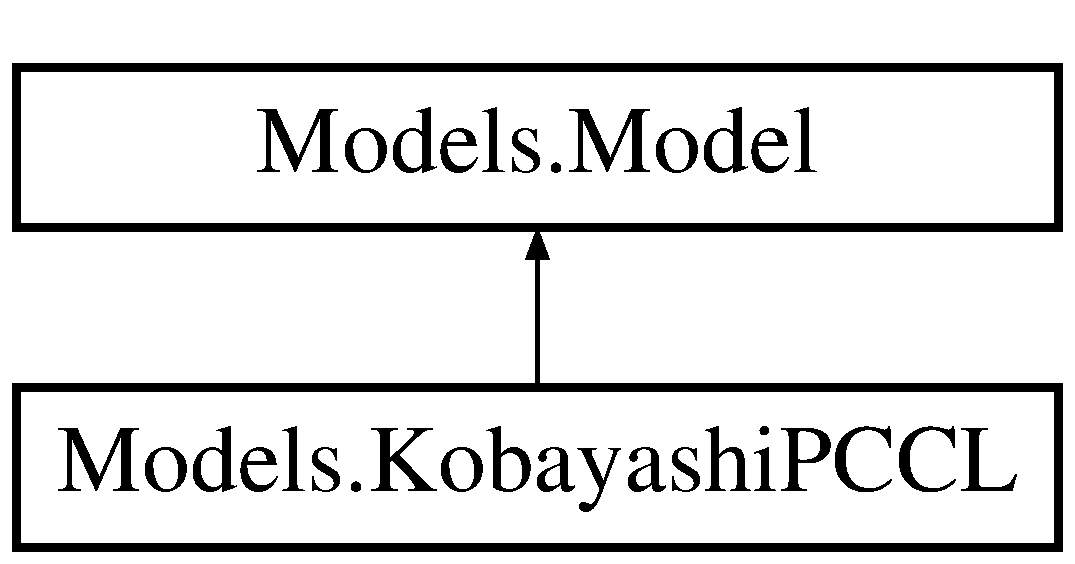
\includegraphics[height=2.000000cm]{classModels_1_1KobayashiPCCL}
\end{center}
\end{figure}
\subsection*{\-Public \-Member \-Functions}
\begin{DoxyCompactItemize}
\item 
\hypertarget{classModels_1_1KobayashiPCCL_a7b363dff31890fad701f0e752b533391}{def {\bfseries \-\_\-\-\_\-init\-\_\-\-\_\-}}\label{classModels_1_1KobayashiPCCL_a7b363dff31890fad701f0e752b533391}

\item 
def \hyperlink{classModels_1_1KobayashiPCCL_a247e1886dafcb2629777bf6feb7d7f4c}{calc\-Mass}
\item 
def \hyperlink{classModels_1_1KobayashiPCCL_ad541181972142ac989d44d0a3b070847}{\-Convert\-Kin\-Factors}
\item 
def \hyperlink{classModels_1_1KobayashiPCCL_a1c7786daeb39d647abbe428adc0f6f03}{set\-Kob\-Weights}
\item 
def \hyperlink{classModels_1_1KobayashiPCCL_a038ff70977e6017b498f584d6a855be1}{\-Kob\-Weights}
\item 
def \hyperlink{classModels_1_1KobayashiPCCL_a30e2e0c8835c4b3cb9a9af52ca9b1fd5}{set\-E2\-Diff}
\item 
def \hyperlink{classModels_1_1KobayashiPCCL_ae26d3a16a364aae97be94e420c897fc4}{\-E2\-Diff}
\item 
def \hyperlink{classModels_1_1Model_a317ed848b969dbe3a96dd05e8b771900}{plt\-Yield}
\item 
def \hyperlink{classModels_1_1Model_aa35c741babf8f141df48c4021e0664e4}{plt\-Rate}
\item 
def \hyperlink{classModels_1_1Model_a3396d6ca1a7b7d66e55ada8c3c7a509e}{max\-Length\-Of\-Vectors}
\item 
def \hyperlink{classModels_1_1Model_ae404a691e48bfe4eafcdfdd09f1dae48}{plot}
\item 
def \hyperlink{classModels_1_1Model_a010945ed2adff59a7a5fce36025e7a97}{derive\-C}
\item 
def \hyperlink{classModels_1_1Model_a7c9280e33f9e0d46703cebc131008c65}{calc\-Rate}
\item 
def \hyperlink{classModels_1_1Model_a818f207e2a4bd0e9a3720ca611960e5a}{set\-Param\-Vector}
\item 
def \hyperlink{classModels_1_1Model_a13c76a0fe24d43cdc4d21fbc73fa96fa}{\-Param\-Vector}
\item 
def \hyperlink{classModels_1_1Model_ad3e627980d9e781bf7b2c9ff900ca06b}{\-Error\-Yield}
\item 
def \hyperlink{classModels_1_1Model_a3050eb39341f318d8d88b172f88bd240}{\-Error\-Rate}
\item 
def \hyperlink{classModels_1_1Model_adcb987bccae63a742490ea1e6d5f7a74}{mk\-Simple\-Result\-Files}
\item 
def \hyperlink{classModels_1_1Model_ac28252ae5cd6b5ecd4c5d006a0e6567d}{set\-Dt4\-Intergrate}
\end{DoxyCompactItemize}
\subsection*{\-Public \-Attributes}
\begin{DoxyCompactItemize}
\item 
\hypertarget{classModels_1_1KobayashiPCCL_a71167eaf1c943b108ca87c51ba8ba310}{{\bfseries \-O\-D\-E\-\_\-hmax}}\label{classModels_1_1KobayashiPCCL_a71167eaf1c943b108ca87c51ba8ba310}

\item 
\hypertarget{classModels_1_1KobayashiPCCL_aa6387b8966d48c2b1c827136ef4a931b}{{\bfseries const\-Dt}}\label{classModels_1_1KobayashiPCCL_aa6387b8966d48c2b1c827136ef4a931b}

\item 
\hypertarget{classModels_1_1KobayashiPCCL_a99a9c55bdcc2446d86ac8533566ec76f}{{\bfseries fgdvc}}\label{classModels_1_1KobayashiPCCL_a99a9c55bdcc2446d86ac8533566ec76f}

\item 
\hypertarget{classModels_1_1Model_a3f71983de5f8b86bec47929213b900ec}{{\bfseries const\-Dt\-Vec}}\label{classModels_1_1Model_a3f71983de5f8b86bec47929213b900ec}

\end{DoxyCompactItemize}


\subsection{\-Detailed \-Description}
\begin{DoxyVerb}Calculates the devolatilization reaction using the Kobayashi model. The Arrhenius equation inside are in the standard notation. The fitting parameter are as in PCCL A1,A2,E1,alpha1. TimeVectorToInterplt allows the option to define the discrete time points, where to interpolate the results. If set to False (standard), then is are the outputted results equal the dt to solve the ODE.\end{DoxyVerb}
 

\subsection{\-Member \-Function \-Documentation}
\hypertarget{classModels_1_1KobayashiPCCL_a247e1886dafcb2629777bf6feb7d7f4c}{\index{\-Models\-::\-Kobayashi\-P\-C\-C\-L@{\-Models\-::\-Kobayashi\-P\-C\-C\-L}!calc\-Mass@{calc\-Mass}}
\index{calc\-Mass@{calc\-Mass}!Models::KobayashiPCCL@{\-Models\-::\-Kobayashi\-P\-C\-C\-L}}
\subsubsection[{calc\-Mass}]{\setlength{\rightskip}{0pt plus 5cm}def {\bf \-Models.\-Kobayashi\-P\-C\-C\-L.\-calc\-Mass} (
\begin{DoxyParamCaption}
\item[{}]{self, }
\item[{}]{fgdvc, }
\item[{}]{time, }
\item[{}]{\-T, }
\item[{}]{\-Name}
\end{DoxyParamCaption}
)}}\label{classModels_1_1KobayashiPCCL_a247e1886dafcb2629777bf6feb7d7f4c}
\begin{DoxyVerb}Outputs the mass(t) using the model specific equation.\end{DoxyVerb}
 \hypertarget{classModels_1_1Model_a7c9280e33f9e0d46703cebc131008c65}{\index{\-Models\-::\-Kobayashi\-P\-C\-C\-L@{\-Models\-::\-Kobayashi\-P\-C\-C\-L}!calc\-Rate@{calc\-Rate}}
\index{calc\-Rate@{calc\-Rate}!Models::KobayashiPCCL@{\-Models\-::\-Kobayashi\-P\-C\-C\-L}}
\subsubsection[{calc\-Rate}]{\setlength{\rightskip}{0pt plus 5cm}def {\bf \-Models.\-Model.\-calc\-Rate} (
\begin{DoxyParamCaption}
\item[{}]{self, }
\item[{}]{fgdvc, }
\item[{}]{time, }
\item[{}]{\-T, }
\item[{}]{\-Name}
\end{DoxyParamCaption}
)\hspace{0.3cm}{\ttfamily  \mbox{[}inherited\mbox{]}}}}\label{classModels_1_1Model_a7c9280e33f9e0d46703cebc131008c65}
\begin{DoxyVerb}Generates the Rates using the yields vector and a CDS.\end{DoxyVerb}
 \hypertarget{classModels_1_1KobayashiPCCL_ad541181972142ac989d44d0a3b070847}{\index{\-Models\-::\-Kobayashi\-P\-C\-C\-L@{\-Models\-::\-Kobayashi\-P\-C\-C\-L}!\-Convert\-Kin\-Factors@{\-Convert\-Kin\-Factors}}
\index{\-Convert\-Kin\-Factors@{\-Convert\-Kin\-Factors}!Models::KobayashiPCCL@{\-Models\-::\-Kobayashi\-P\-C\-C\-L}}
\subsubsection[{\-Convert\-Kin\-Factors}]{\setlength{\rightskip}{0pt plus 5cm}def {\bf \-Models.\-Kobayashi\-P\-C\-C\-L.\-Convert\-Kin\-Factors} (
\begin{DoxyParamCaption}
\item[{}]{self, }
\item[{}]{\-Parameter\-Vector}
\end{DoxyParamCaption}
)}}\label{classModels_1_1KobayashiPCCL_ad541181972142ac989d44d0a3b070847}
\begin{DoxyVerb}Outputs the Arrhenius equation factors in the shape [A1,E1,A2,E2]. Here where the real Arrhenius model is in use only a dummy function.\end{DoxyVerb}
 \hypertarget{classModels_1_1Model_a010945ed2adff59a7a5fce36025e7a97}{\index{\-Models\-::\-Kobayashi\-P\-C\-C\-L@{\-Models\-::\-Kobayashi\-P\-C\-C\-L}!derive\-C@{derive\-C}}
\index{derive\-C@{derive\-C}!Models::KobayashiPCCL@{\-Models\-::\-Kobayashi\-P\-C\-C\-L}}
\subsubsection[{derive\-C}]{\setlength{\rightskip}{0pt plus 5cm}def {\bf \-Models.\-Model.\-derive\-C} (
\begin{DoxyParamCaption}
\item[{}]{self, }
\item[{}]{fgdvc, }
\item[{}]{y\-Vector}
\end{DoxyParamCaption}
)\hspace{0.3cm}{\ttfamily  \mbox{[}inherited\mbox{]}}}}\label{classModels_1_1Model_a010945ed2adff59a7a5fce36025e7a97}
\begin{DoxyVerb}Returns a CDS of the inputted yVector.\end{DoxyVerb}
 \hypertarget{classModels_1_1KobayashiPCCL_ae26d3a16a364aae97be94e420c897fc4}{\index{\-Models\-::\-Kobayashi\-P\-C\-C\-L@{\-Models\-::\-Kobayashi\-P\-C\-C\-L}!\-E2\-Diff@{\-E2\-Diff}}
\index{\-E2\-Diff@{\-E2\-Diff}!Models::KobayashiPCCL@{\-Models\-::\-Kobayashi\-P\-C\-C\-L}}
\subsubsection[{\-E2\-Diff}]{\setlength{\rightskip}{0pt plus 5cm}def {\bf \-Models.\-Kobayashi\-P\-C\-C\-L.\-E2\-Diff} (
\begin{DoxyParamCaption}
\item[{}]{self}
\end{DoxyParamCaption}
)}}\label{classModels_1_1KobayashiPCCL_ae26d3a16a364aae97be94e420c897fc4}
\begin{DoxyVerb}Returns the dE in E2=E1+dE.\end{DoxyVerb}
 \hypertarget{classModels_1_1Model_a3050eb39341f318d8d88b172f88bd240}{\index{\-Models\-::\-Kobayashi\-P\-C\-C\-L@{\-Models\-::\-Kobayashi\-P\-C\-C\-L}!\-Error\-Rate@{\-Error\-Rate}}
\index{\-Error\-Rate@{\-Error\-Rate}!Models::KobayashiPCCL@{\-Models\-::\-Kobayashi\-P\-C\-C\-L}}
\subsubsection[{\-Error\-Rate}]{\setlength{\rightskip}{0pt plus 5cm}def {\bf \-Models.\-Model.\-Error\-Rate} (
\begin{DoxyParamCaption}
\item[{}]{self, }
\item[{}]{fgdvc, }
\item[{}]{\-Species}
\end{DoxyParamCaption}
)\hspace{0.3cm}{\ttfamily  \mbox{[}inherited\mbox{]}}}}\label{classModels_1_1Model_a3050eb39341f318d8d88b172f88bd240}
\begin{DoxyVerb}Returns the absolute deviation per point between the fitted and the original rate curve.\end{DoxyVerb}
 \hypertarget{classModels_1_1Model_ad3e627980d9e781bf7b2c9ff900ca06b}{\index{\-Models\-::\-Kobayashi\-P\-C\-C\-L@{\-Models\-::\-Kobayashi\-P\-C\-C\-L}!\-Error\-Yield@{\-Error\-Yield}}
\index{\-Error\-Yield@{\-Error\-Yield}!Models::KobayashiPCCL@{\-Models\-::\-Kobayashi\-P\-C\-C\-L}}
\subsubsection[{\-Error\-Yield}]{\setlength{\rightskip}{0pt plus 5cm}def {\bf \-Models.\-Model.\-Error\-Yield} (
\begin{DoxyParamCaption}
\item[{}]{self, }
\item[{}]{fgdvc, }
\item[{}]{\-Species}
\end{DoxyParamCaption}
)\hspace{0.3cm}{\ttfamily  \mbox{[}inherited\mbox{]}}}}\label{classModels_1_1Model_ad3e627980d9e781bf7b2c9ff900ca06b}
\begin{DoxyVerb}Returns the absolute deviation per point between the fitted and the original yield curve.\end{DoxyVerb}
 \hypertarget{classModels_1_1KobayashiPCCL_a038ff70977e6017b498f584d6a855be1}{\index{\-Models\-::\-Kobayashi\-P\-C\-C\-L@{\-Models\-::\-Kobayashi\-P\-C\-C\-L}!\-Kob\-Weights@{\-Kob\-Weights}}
\index{\-Kob\-Weights@{\-Kob\-Weights}!Models::KobayashiPCCL@{\-Models\-::\-Kobayashi\-P\-C\-C\-L}}
\subsubsection[{\-Kob\-Weights}]{\setlength{\rightskip}{0pt plus 5cm}def {\bf \-Models.\-Kobayashi\-P\-C\-C\-L.\-Kob\-Weights} (
\begin{DoxyParamCaption}
\item[{}]{self}
\end{DoxyParamCaption}
)}}\label{classModels_1_1KobayashiPCCL_a038ff70977e6017b498f584d6a855be1}
\begin{DoxyVerb}Returns the two Kobayashi weights alpha2.\end{DoxyVerb}
 \hypertarget{classModels_1_1Model_a3396d6ca1a7b7d66e55ada8c3c7a509e}{\index{\-Models\-::\-Kobayashi\-P\-C\-C\-L@{\-Models\-::\-Kobayashi\-P\-C\-C\-L}!max\-Length\-Of\-Vectors@{max\-Length\-Of\-Vectors}}
\index{max\-Length\-Of\-Vectors@{max\-Length\-Of\-Vectors}!Models::KobayashiPCCL@{\-Models\-::\-Kobayashi\-P\-C\-C\-L}}
\subsubsection[{max\-Length\-Of\-Vectors}]{\setlength{\rightskip}{0pt plus 5cm}def {\bf \-Models.\-Model.\-max\-Length\-Of\-Vectors} (
\begin{DoxyParamCaption}
\item[{}]{self, }
\item[{}]{fgdvc\-\_\-list}
\end{DoxyParamCaption}
)\hspace{0.3cm}{\ttfamily  \mbox{[}inherited\mbox{]}}}}\label{classModels_1_1Model_a3396d6ca1a7b7d66e55ada8c3c7a509e}
\begin{DoxyVerb}Returns the minimum lenght of a all vectors from the several runs.\end{DoxyVerb}
 \hypertarget{classModels_1_1Model_adcb987bccae63a742490ea1e6d5f7a74}{\index{\-Models\-::\-Kobayashi\-P\-C\-C\-L@{\-Models\-::\-Kobayashi\-P\-C\-C\-L}!mk\-Simple\-Result\-Files@{mk\-Simple\-Result\-Files}}
\index{mk\-Simple\-Result\-Files@{mk\-Simple\-Result\-Files}!Models::KobayashiPCCL@{\-Models\-::\-Kobayashi\-P\-C\-C\-L}}
\subsubsection[{mk\-Simple\-Result\-Files}]{\setlength{\rightskip}{0pt plus 5cm}def {\bf \-Models.\-Model.\-mk\-Simple\-Result\-Files} (
\begin{DoxyParamCaption}
\item[{}]{self, }
\item[{}]{fgdvc\-\_\-list, }
\item[{}]{\-Species}
\end{DoxyParamCaption}
)\hspace{0.3cm}{\ttfamily  \mbox{[}inherited\mbox{]}}}}\label{classModels_1_1Model_adcb987bccae63a742490ea1e6d5f7a74}
\begin{DoxyVerb}Simple result file if no fitting is carried out. Writes only the transformed results into a file.\end{DoxyVerb}
 \hypertarget{classModels_1_1Model_a13c76a0fe24d43cdc4d21fbc73fa96fa}{\index{\-Models\-::\-Kobayashi\-P\-C\-C\-L@{\-Models\-::\-Kobayashi\-P\-C\-C\-L}!\-Param\-Vector@{\-Param\-Vector}}
\index{\-Param\-Vector@{\-Param\-Vector}!Models::KobayashiPCCL@{\-Models\-::\-Kobayashi\-P\-C\-C\-L}}
\subsubsection[{\-Param\-Vector}]{\setlength{\rightskip}{0pt plus 5cm}def {\bf \-Models.\-Model.\-Param\-Vector} (
\begin{DoxyParamCaption}
\item[{}]{self}
\end{DoxyParamCaption}
)\hspace{0.3cm}{\ttfamily  \mbox{[}inherited\mbox{]}}}}\label{classModels_1_1Model_a13c76a0fe24d43cdc4d21fbc73fa96fa}
\begin{DoxyVerb}Returns the Vector containing the kinetic parameter of the Model (refering to the child model).\end{DoxyVerb}
 \hypertarget{classModels_1_1Model_ae404a691e48bfe4eafcdfdd09f1dae48}{\index{\-Models\-::\-Kobayashi\-P\-C\-C\-L@{\-Models\-::\-Kobayashi\-P\-C\-C\-L}!plot@{plot}}
\index{plot@{plot}!Models::KobayashiPCCL@{\-Models\-::\-Kobayashi\-P\-C\-C\-L}}
\subsubsection[{plot}]{\setlength{\rightskip}{0pt plus 5cm}def {\bf \-Models.\-Model.\-plot} (
\begin{DoxyParamCaption}
\item[{}]{self, }
\item[{}]{fgdvc\-\_\-list, }
\item[{}]{\-Species}
\end{DoxyParamCaption}
)\hspace{0.3cm}{\ttfamily  \mbox{[}inherited\mbox{]}}}}\label{classModels_1_1Model_ae404a691e48bfe4eafcdfdd09f1dae48}
\begin{DoxyVerb}Plot the yield and the rates over time with two curves: one is the original data, the other the fitting curve. Also file 'PyrolysisProgramName-Species.out' (e.g. 'CPD-CO2.out') containing the time (s), yields (kg/kg), rates (kg/(kg s)).\end{DoxyVerb}
 \hypertarget{classModels_1_1Model_aa35c741babf8f141df48c4021e0664e4}{\index{\-Models\-::\-Kobayashi\-P\-C\-C\-L@{\-Models\-::\-Kobayashi\-P\-C\-C\-L}!plt\-Rate@{plt\-Rate}}
\index{plt\-Rate@{plt\-Rate}!Models::KobayashiPCCL@{\-Models\-::\-Kobayashi\-P\-C\-C\-L}}
\subsubsection[{plt\-Rate}]{\setlength{\rightskip}{0pt plus 5cm}def {\bf \-Models.\-Model.\-plt\-Rate} (
\begin{DoxyParamCaption}
\item[{}]{self, }
\item[{}]{fgdvc\-\_\-list, }
\item[{}]{x\-Value\-To\-Plot, }
\item[{}]{y\-Value\-To\-Plot}
\end{DoxyParamCaption}
)\hspace{0.3cm}{\ttfamily  \mbox{[}inherited\mbox{]}}}}\label{classModels_1_1Model_aa35c741babf8f141df48c4021e0664e4}
\begin{DoxyVerb}Plots the rates (to select with yValueToPlot) over Time or Temperature (to slect with xValueToPlot).\end{DoxyVerb}
 \hypertarget{classModels_1_1Model_a317ed848b969dbe3a96dd05e8b771900}{\index{\-Models\-::\-Kobayashi\-P\-C\-C\-L@{\-Models\-::\-Kobayashi\-P\-C\-C\-L}!plt\-Yield@{plt\-Yield}}
\index{plt\-Yield@{plt\-Yield}!Models::KobayashiPCCL@{\-Models\-::\-Kobayashi\-P\-C\-C\-L}}
\subsubsection[{plt\-Yield}]{\setlength{\rightskip}{0pt plus 5cm}def {\bf \-Models.\-Model.\-plt\-Yield} (
\begin{DoxyParamCaption}
\item[{}]{self, }
\item[{}]{fgdvc\-\_\-list, }
\item[{}]{x\-Value\-To\-Plot, }
\item[{}]{y\-Value\-To\-Plot}
\end{DoxyParamCaption}
)\hspace{0.3cm}{\ttfamily  \mbox{[}inherited\mbox{]}}}}\label{classModels_1_1Model_a317ed848b969dbe3a96dd05e8b771900}
\begin{DoxyVerb}Plots the yields (to select with yValueToPlot) over Time or Temperature (to slect with xValueToPlot).\end{DoxyVerb}
 \hypertarget{classModels_1_1Model_ac28252ae5cd6b5ecd4c5d006a0e6567d}{\index{\-Models\-::\-Kobayashi\-P\-C\-C\-L@{\-Models\-::\-Kobayashi\-P\-C\-C\-L}!set\-Dt4\-Intergrate@{set\-Dt4\-Intergrate}}
\index{set\-Dt4\-Intergrate@{set\-Dt4\-Intergrate}!Models::KobayashiPCCL@{\-Models\-::\-Kobayashi\-P\-C\-C\-L}}
\subsubsection[{set\-Dt4\-Intergrate}]{\setlength{\rightskip}{0pt plus 5cm}def {\bf \-Models.\-Model.\-set\-Dt4\-Intergrate} (
\begin{DoxyParamCaption}
\item[{}]{self, }
\item[{}]{constant\-Dt}
\end{DoxyParamCaption}
)\hspace{0.3cm}{\ttfamily  \mbox{[}inherited\mbox{]}}}}\label{classModels_1_1Model_ac28252ae5cd6b5ecd4c5d006a0e6567d}
\begin{DoxyVerb}constantDt allows the option to define numerical time step to solve the ODE. The outputted results ever equal the imported time list (when applying method calcMass Time = [t0,t1,t2,t3,t4]. If these time steps are too large, then is this defined dt used to solve the ODE and the results are linear interploated that way that they correspond to the imported time vector. To reset it, just set constantDt to False.\end{DoxyVerb}
 \hypertarget{classModels_1_1KobayashiPCCL_a30e2e0c8835c4b3cb9a9af52ca9b1fd5}{\index{\-Models\-::\-Kobayashi\-P\-C\-C\-L@{\-Models\-::\-Kobayashi\-P\-C\-C\-L}!set\-E2\-Diff@{set\-E2\-Diff}}
\index{set\-E2\-Diff@{set\-E2\-Diff}!Models::KobayashiPCCL@{\-Models\-::\-Kobayashi\-P\-C\-C\-L}}
\subsubsection[{set\-E2\-Diff}]{\setlength{\rightskip}{0pt plus 5cm}def {\bf \-Models.\-Kobayashi\-P\-C\-C\-L.\-set\-E2\-Diff} (
\begin{DoxyParamCaption}
\item[{}]{self, }
\item[{}]{\-Difference\-E1\-E2}
\end{DoxyParamCaption}
)}}\label{classModels_1_1KobayashiPCCL_a30e2e0c8835c4b3cb9a9af52ca9b1fd5}
\begin{DoxyVerb}Sets the dE in E2=E1+dE.\end{DoxyVerb}
 \hypertarget{classModels_1_1KobayashiPCCL_a1c7786daeb39d647abbe428adc0f6f03}{\index{\-Models\-::\-Kobayashi\-P\-C\-C\-L@{\-Models\-::\-Kobayashi\-P\-C\-C\-L}!set\-Kob\-Weights@{set\-Kob\-Weights}}
\index{set\-Kob\-Weights@{set\-Kob\-Weights}!Models::KobayashiPCCL@{\-Models\-::\-Kobayashi\-P\-C\-C\-L}}
\subsubsection[{set\-Kob\-Weights}]{\setlength{\rightskip}{0pt plus 5cm}def {\bf \-Models.\-Kobayashi\-P\-C\-C\-L.\-set\-Kob\-Weights} (
\begin{DoxyParamCaption}
\item[{}]{self, }
\item[{}]{alpha2}
\end{DoxyParamCaption}
)}}\label{classModels_1_1KobayashiPCCL_a1c7786daeb39d647abbe428adc0f6f03}
\begin{DoxyVerb}Sets the two Kobayashi weights alpha2.\end{DoxyVerb}
 \hypertarget{classModels_1_1Model_a818f207e2a4bd0e9a3720ca611960e5a}{\index{\-Models\-::\-Kobayashi\-P\-C\-C\-L@{\-Models\-::\-Kobayashi\-P\-C\-C\-L}!set\-Param\-Vector@{set\-Param\-Vector}}
\index{set\-Param\-Vector@{set\-Param\-Vector}!Models::KobayashiPCCL@{\-Models\-::\-Kobayashi\-P\-C\-C\-L}}
\subsubsection[{set\-Param\-Vector}]{\setlength{\rightskip}{0pt plus 5cm}def {\bf \-Models.\-Model.\-set\-Param\-Vector} (
\begin{DoxyParamCaption}
\item[{}]{self, }
\item[{}]{\-Parameter\-List}
\end{DoxyParamCaption}
)\hspace{0.3cm}{\ttfamily  \mbox{[}inherited\mbox{]}}}}\label{classModels_1_1Model_a818f207e2a4bd0e9a3720ca611960e5a}
\begin{DoxyVerb}Sets the Vector containing the kinetic parameter of the Model (refering to the child model).\end{DoxyVerb}
 

\-The documentation for this class was generated from the following file\-:\begin{DoxyCompactItemize}
\item 
/home/map/git/pkp/src/\-Models.\-py\end{DoxyCompactItemize}

\hypertarget{classFitter_1_1LeastSquarsEstimator}{\section{\-Fitter.\-Least\-Squars\-Estimator \-Class \-Reference}
\label{classFitter_1_1LeastSquarsEstimator}\index{\-Fitter.\-Least\-Squars\-Estimator@{\-Fitter.\-Least\-Squars\-Estimator}}
}
\subsection*{\-Public \-Member \-Functions}
\begin{DoxyCompactItemize}
\item 
\hypertarget{classFitter_1_1LeastSquarsEstimator_aea7092ad8516d452c695b8ed01634029}{def {\bfseries \-\_\-\-\_\-init\-\_\-\-\_\-}}\label{classFitter_1_1LeastSquarsEstimator_aea7092ad8516d452c695b8ed01634029}

\item 
def \hyperlink{classFitter_1_1LeastSquarsEstimator_aff91169bf33f8f810b1e98ac98a23c62}{improve\-\_\-\-E}
\item 
def \hyperlink{classFitter_1_1LeastSquarsEstimator_a15492452ccc16caf31bf234bcc702a5d}{improve\-\_\-a}
\item 
def \hyperlink{classFitter_1_1LeastSquarsEstimator_a25552eed081a2291c17fe1fda3896cd1}{max\-Length\-Of\-Vectors}
\item 
def \hyperlink{classFitter_1_1LeastSquarsEstimator_adb70f7a05a5bfff482f2d45634960032}{estimate\-\_\-\-T}
\item 
def \hyperlink{classFitter_1_1LeastSquarsEstimator_a90144e4465eb66adf978126a2d09ff54}{\-Deviation}
\item 
def \hyperlink{classFitter_1_1LeastSquarsEstimator_a9c94ff877c2bc358faf8feafb73c3f97}{set\-Weights}
\item 
def \hyperlink{classFitter_1_1LeastSquarsEstimator_abf4a0423ab282f5ebd1e881f94549bce}{set\-Tolerance}
\item 
def \hyperlink{classFitter_1_1LeastSquarsEstimator_aef4c901e6afb654ad2b70bc2960ecadb}{set\-Pre\-Tolerance}
\item 
def \hyperlink{classFitter_1_1LeastSquarsEstimator_a9911d334b53c772a18afba9cb1e54113}{set\-Pre\-Max\-Iter}
\item 
def \hyperlink{classFitter_1_1LeastSquarsEstimator_ab06c721baf4cc0e88ef99b60479080c9}{set\-Max\-Iter}
\item 
def \hyperlink{classFitter_1_1LeastSquarsEstimator_a72a06037b1cfde39955fc412ace06134}{set\-Optimizer}
\item 
def \hyperlink{classFitter_1_1LeastSquarsEstimator_acd0fa0e003dabe354ceb4e0f2fec15ac}{set\-Final\-Yield}
\end{DoxyCompactItemize}
\subsection*{\-Public \-Attributes}
\begin{DoxyCompactItemize}
\item 
\hypertarget{classFitter_1_1LeastSquarsEstimator_ad969e6101168c73a3939523ecd7fa8f7}{{\bfseries \-Pre\-\_\-\-Tolerance}}\label{classFitter_1_1LeastSquarsEstimator_ad969e6101168c73a3939523ecd7fa8f7}

\item 
\hypertarget{classFitter_1_1LeastSquarsEstimator_a85c98dc2151ad5f2fbdef6a1401e70ef}{{\bfseries \-Fit\-\_\-\-Tolerance}}\label{classFitter_1_1LeastSquarsEstimator_a85c98dc2151ad5f2fbdef6a1401e70ef}

\item 
\hypertarget{classFitter_1_1LeastSquarsEstimator_af20a1616ebc0ce9ed3cc009e4835f066}{{\bfseries \-Pre\-Max\-Iter}}\label{classFitter_1_1LeastSquarsEstimator_af20a1616ebc0ce9ed3cc009e4835f066}

\item 
\hypertarget{classFitter_1_1LeastSquarsEstimator_a680631df2fc3dea042fc1d8d356cd2b0}{{\bfseries \-Max\-Iter}}\label{classFitter_1_1LeastSquarsEstimator_a680631df2fc3dea042fc1d8d356cd2b0}

\item 
\hypertarget{classFitter_1_1LeastSquarsEstimator_a9ca4568ab77f2598ae741c10ec32111d}{{\bfseries \-Final\-Y}}\label{classFitter_1_1LeastSquarsEstimator_a9ca4568ab77f2598ae741c10ec32111d}

\item 
\hypertarget{classFitter_1_1LeastSquarsEstimator_a3d5a4e3561f38dc77c6f410442b3dc56}{\hyperlink{classFitter_1_1LeastSquarsEstimator_a3d5a4e3561f38dc77c6f410442b3dc56}{selected\-Optimizer}}\label{classFitter_1_1LeastSquarsEstimator_a3d5a4e3561f38dc77c6f410442b3dc56}

\begin{DoxyCompactList}\small\item\em scaled weight factor \end{DoxyCompactList}\item 
\hypertarget{classFitter_1_1LeastSquarsEstimator_ad879a97226028a55bc21ddcc30915e2f}{{\bfseries \-Final\-Deviation}}\label{classFitter_1_1LeastSquarsEstimator_ad879a97226028a55bc21ddcc30915e2f}

\item 
\hypertarget{classFitter_1_1LeastSquarsEstimator_a132cc0f4395b7d97a12e0cd1774c82d0}{{\bfseries a0}}\label{classFitter_1_1LeastSquarsEstimator_a132cc0f4395b7d97a12e0cd1774c82d0}

\item 
\hypertarget{classFitter_1_1LeastSquarsEstimator_a5dad5e4a0688e961472acb32259ed5ae}{{\bfseries a1}}\label{classFitter_1_1LeastSquarsEstimator_a5dad5e4a0688e961472acb32259ed5ae}

\end{DoxyCompactItemize}


\subsection{\-Detailed \-Description}
\begin{DoxyVerb}Optimizes the Fitting curve using the Least Squares for the Yields and the Rates.\end{DoxyVerb}
 

\subsection{\-Member \-Function \-Documentation}
\hypertarget{classFitter_1_1LeastSquarsEstimator_a90144e4465eb66adf978126a2d09ff54}{\index{\-Fitter\-::\-Least\-Squars\-Estimator@{\-Fitter\-::\-Least\-Squars\-Estimator}!\-Deviation@{\-Deviation}}
\index{\-Deviation@{\-Deviation}!Fitter::LeastSquarsEstimator@{\-Fitter\-::\-Least\-Squars\-Estimator}}
\subsubsection[{\-Deviation}]{\setlength{\rightskip}{0pt plus 5cm}def {\bf \-Fitter.\-Least\-Squars\-Estimator.\-Deviation} (
\begin{DoxyParamCaption}
\item[{}]{self}
\end{DoxyParamCaption}
)}}\label{classFitter_1_1LeastSquarsEstimator_a90144e4465eb66adf978126a2d09ff54}
\begin{DoxyVerb}Returns the Deviation after the optimization procedure.\end{DoxyVerb}
 \hypertarget{classFitter_1_1LeastSquarsEstimator_adb70f7a05a5bfff482f2d45634960032}{\index{\-Fitter\-::\-Least\-Squars\-Estimator@{\-Fitter\-::\-Least\-Squars\-Estimator}!estimate\-\_\-\-T@{estimate\-\_\-\-T}}
\index{estimate\-\_\-\-T@{estimate\-\_\-\-T}!Fitter::LeastSquarsEstimator@{\-Fitter\-::\-Least\-Squars\-Estimator}}
\subsubsection[{estimate\-\_\-\-T}]{\setlength{\rightskip}{0pt plus 5cm}def {\bf \-Fitter.\-Least\-Squars\-Estimator.\-estimate\-\_\-\-T} (
\begin{DoxyParamCaption}
\item[{}]{self, }
\item[{}]{fgdvc\-\_\-list, }
\item[{}]{model, }
\item[{}]{\-Parameter\-\_\-\-Vector, }
\item[{}]{\-Name, }
\item[{}]{pre\-Loop\-Number = {\ttfamily 0}}
\end{DoxyParamCaption}
)}}\label{classFitter_1_1LeastSquarsEstimator_adb70f7a05a5bfff482f2d45634960032}
\begin{DoxyVerb}The main optimization method. Optimizes the Fitting curve using the Least Squares for the weighted Yields and the weighted Rates considering the temperatur history. Requires at input: The corresponding Fit_one_run object, the Model object, the kinetic parameter list, a name (e.g. the species). preLoopNumber is the number of running the  improve_E and improve_a routines. So the standard setting of preLoopNumber is equal zero. It may be used if there is only a very bad convergence when optimize all three parameter.\end{DoxyVerb}
 \hypertarget{classFitter_1_1LeastSquarsEstimator_a15492452ccc16caf31bf234bcc702a5d}{\index{\-Fitter\-::\-Least\-Squars\-Estimator@{\-Fitter\-::\-Least\-Squars\-Estimator}!improve\-\_\-a@{improve\-\_\-a}}
\index{improve\-\_\-a@{improve\-\_\-a}!Fitter::LeastSquarsEstimator@{\-Fitter\-::\-Least\-Squars\-Estimator}}
\subsubsection[{improve\-\_\-a}]{\setlength{\rightskip}{0pt plus 5cm}def {\bf \-Fitter.\-Least\-Squars\-Estimator.\-improve\-\_\-a} (
\begin{DoxyParamCaption}
\item[{}]{self, }
\item[{}]{fgdvc, }
\item[{}]{model, }
\item[{}]{t, }
\item[{}]{\-T, }
\item[{}]{\-Parameter\-\_\-\-Vector, }
\item[{}]{\-Name}
\end{DoxyParamCaption}
)}}\label{classFitter_1_1LeastSquarsEstimator_a15492452ccc16caf31bf234bcc702a5d}
\begin{DoxyVerb}Additional option: Only the preexponential factor in the Arrhenius Equation is optimized. Actual not necessary.\end{DoxyVerb}
 \hypertarget{classFitter_1_1LeastSquarsEstimator_aff91169bf33f8f810b1e98ac98a23c62}{\index{\-Fitter\-::\-Least\-Squars\-Estimator@{\-Fitter\-::\-Least\-Squars\-Estimator}!improve\-\_\-\-E@{improve\-\_\-\-E}}
\index{improve\-\_\-\-E@{improve\-\_\-\-E}!Fitter::LeastSquarsEstimator@{\-Fitter\-::\-Least\-Squars\-Estimator}}
\subsubsection[{improve\-\_\-\-E}]{\setlength{\rightskip}{0pt plus 5cm}def {\bf \-Fitter.\-Least\-Squars\-Estimator.\-improve\-\_\-\-E} (
\begin{DoxyParamCaption}
\item[{}]{self, }
\item[{}]{fgdvc, }
\item[{}]{model, }
\item[{}]{t, }
\item[{}]{\-T, }
\item[{}]{\-Parameter\-\_\-\-Vector, }
\item[{}]{\-Name}
\end{DoxyParamCaption}
)}}\label{classFitter_1_1LeastSquarsEstimator_aff91169bf33f8f810b1e98ac98a23c62}
\begin{DoxyVerb}Additional option: Only the Activation Energy in the Arrhenius Equation is optimized. Actual not necessary.\end{DoxyVerb}
 \hypertarget{classFitter_1_1LeastSquarsEstimator_a25552eed081a2291c17fe1fda3896cd1}{\index{\-Fitter\-::\-Least\-Squars\-Estimator@{\-Fitter\-::\-Least\-Squars\-Estimator}!max\-Length\-Of\-Vectors@{max\-Length\-Of\-Vectors}}
\index{max\-Length\-Of\-Vectors@{max\-Length\-Of\-Vectors}!Fitter::LeastSquarsEstimator@{\-Fitter\-::\-Least\-Squars\-Estimator}}
\subsubsection[{max\-Length\-Of\-Vectors}]{\setlength{\rightskip}{0pt plus 5cm}def {\bf \-Fitter.\-Least\-Squars\-Estimator.\-max\-Length\-Of\-Vectors} (
\begin{DoxyParamCaption}
\item[{}]{self, }
\item[{}]{fgdvc\-\_\-list}
\end{DoxyParamCaption}
)}}\label{classFitter_1_1LeastSquarsEstimator_a25552eed081a2291c17fe1fda3896cd1}
\begin{DoxyVerb}Returns the minimum lenght of a all vectors from the several runs.\end{DoxyVerb}
 \hypertarget{classFitter_1_1LeastSquarsEstimator_acd0fa0e003dabe354ceb4e0f2fec15ac}{\index{\-Fitter\-::\-Least\-Squars\-Estimator@{\-Fitter\-::\-Least\-Squars\-Estimator}!set\-Final\-Yield@{set\-Final\-Yield}}
\index{set\-Final\-Yield@{set\-Final\-Yield}!Fitter::LeastSquarsEstimator@{\-Fitter\-::\-Least\-Squars\-Estimator}}
\subsubsection[{set\-Final\-Yield}]{\setlength{\rightskip}{0pt plus 5cm}def {\bf \-Fitter.\-Least\-Squars\-Estimator.\-set\-Final\-Yield} (
\begin{DoxyParamCaption}
\item[{}]{self, }
\item[{}]{\-Final\-Yield}
\end{DoxyParamCaption}
)}}\label{classFitter_1_1LeastSquarsEstimator_acd0fa0e003dabe354ceb4e0f2fec15ac}
\begin{DoxyVerb}Sets the final yield for the ODE to optimize. Enter False if model is Kobayashi equation (independend of final yield,standard Setting). Must be applied for all models except the Kobayashi model.\end{DoxyVerb}
 \hypertarget{classFitter_1_1LeastSquarsEstimator_ab06c721baf4cc0e88ef99b60479080c9}{\index{\-Fitter\-::\-Least\-Squars\-Estimator@{\-Fitter\-::\-Least\-Squars\-Estimator}!set\-Max\-Iter@{set\-Max\-Iter}}
\index{set\-Max\-Iter@{set\-Max\-Iter}!Fitter::LeastSquarsEstimator@{\-Fitter\-::\-Least\-Squars\-Estimator}}
\subsubsection[{set\-Max\-Iter}]{\setlength{\rightskip}{0pt plus 5cm}def {\bf \-Fitter.\-Least\-Squars\-Estimator.\-set\-Max\-Iter} (
\begin{DoxyParamCaption}
\item[{}]{self, }
\item[{}]{\-Maxium\-Number\-Of\-Iteration\-In\-Main\-Procedure}
\end{DoxyParamCaption}
)}}\label{classFitter_1_1LeastSquarsEstimator_ab06c721baf4cc0e88ef99b60479080c9}
\begin{DoxyVerb}Sets the maximum number of iteration oin the optimizer as a abort criterion for the fitting procedure.\end{DoxyVerb}
 \hypertarget{classFitter_1_1LeastSquarsEstimator_a72a06037b1cfde39955fc412ace06134}{\index{\-Fitter\-::\-Least\-Squars\-Estimator@{\-Fitter\-::\-Least\-Squars\-Estimator}!set\-Optimizer@{set\-Optimizer}}
\index{set\-Optimizer@{set\-Optimizer}!Fitter::LeastSquarsEstimator@{\-Fitter\-::\-Least\-Squars\-Estimator}}
\subsubsection[{set\-Optimizer}]{\setlength{\rightskip}{0pt plus 5cm}def {\bf \-Fitter.\-Least\-Squars\-Estimator.\-set\-Optimizer} (
\begin{DoxyParamCaption}
\item[{}]{self, }
\item[{}]{\-Chosen\-Optimizer}
\end{DoxyParamCaption}
)}}\label{classFitter_1_1LeastSquarsEstimator_a72a06037b1cfde39955fc412ace06134}
\begin{DoxyVerb}Select one optimizer of the scipy.optimizer library: 'fmin','fmin_cg','fmin_bfgs','fmin_ncg','fmin_slsqp' or 'leastsq'. According to experience 'fmin' (or also 'leastsq') generates at best the results.\end{DoxyVerb}
 \hypertarget{classFitter_1_1LeastSquarsEstimator_a9911d334b53c772a18afba9cb1e54113}{\index{\-Fitter\-::\-Least\-Squars\-Estimator@{\-Fitter\-::\-Least\-Squars\-Estimator}!set\-Pre\-Max\-Iter@{set\-Pre\-Max\-Iter}}
\index{set\-Pre\-Max\-Iter@{set\-Pre\-Max\-Iter}!Fitter::LeastSquarsEstimator@{\-Fitter\-::\-Least\-Squars\-Estimator}}
\subsubsection[{set\-Pre\-Max\-Iter}]{\setlength{\rightskip}{0pt plus 5cm}def {\bf \-Fitter.\-Least\-Squars\-Estimator.\-set\-Pre\-Max\-Iter} (
\begin{DoxyParamCaption}
\item[{}]{self, }
\item[{}]{\-Maxium\-Number\-Of\-Iteration\-In\-Pre\-Procedure}
\end{DoxyParamCaption}
)}}\label{classFitter_1_1LeastSquarsEstimator_a9911d334b53c772a18afba9cb1e54113}
\begin{DoxyVerb}Sets the maximum number of iteration oin the optimizer as a abort criterion for the prefitting procedure (if preLoopNumber in estimate_T is not equal zero).\end{DoxyVerb}
 \hypertarget{classFitter_1_1LeastSquarsEstimator_aef4c901e6afb654ad2b70bc2960ecadb}{\index{\-Fitter\-::\-Least\-Squars\-Estimator@{\-Fitter\-::\-Least\-Squars\-Estimator}!set\-Pre\-Tolerance@{set\-Pre\-Tolerance}}
\index{set\-Pre\-Tolerance@{set\-Pre\-Tolerance}!Fitter::LeastSquarsEstimator@{\-Fitter\-::\-Least\-Squars\-Estimator}}
\subsubsection[{set\-Pre\-Tolerance}]{\setlength{\rightskip}{0pt plus 5cm}def {\bf \-Fitter.\-Least\-Squars\-Estimator.\-set\-Pre\-Tolerance} (
\begin{DoxyParamCaption}
\item[{}]{self, }
\item[{}]{\-Tolerance\-For\-Fmin\-Function}
\end{DoxyParamCaption}
)}}\label{classFitter_1_1LeastSquarsEstimator_aef4c901e6afb654ad2b70bc2960ecadb}
\begin{DoxyVerb}Sets the tolerance as a abort criterion for the prefitting procedure (if preLoopNumber in estimate_T is not equal zero).\end{DoxyVerb}
 \hypertarget{classFitter_1_1LeastSquarsEstimator_abf4a0423ab282f5ebd1e881f94549bce}{\index{\-Fitter\-::\-Least\-Squars\-Estimator@{\-Fitter\-::\-Least\-Squars\-Estimator}!set\-Tolerance@{set\-Tolerance}}
\index{set\-Tolerance@{set\-Tolerance}!Fitter::LeastSquarsEstimator@{\-Fitter\-::\-Least\-Squars\-Estimator}}
\subsubsection[{set\-Tolerance}]{\setlength{\rightskip}{0pt plus 5cm}def {\bf \-Fitter.\-Least\-Squars\-Estimator.\-set\-Tolerance} (
\begin{DoxyParamCaption}
\item[{}]{self, }
\item[{}]{\-Tolerance\-For\-Fmin\-Function}
\end{DoxyParamCaption}
)}}\label{classFitter_1_1LeastSquarsEstimator_abf4a0423ab282f5ebd1e881f94549bce}
\begin{DoxyVerb}Sets the tolerance as a abort criterion for the fitting procedure.\end{DoxyVerb}
 \hypertarget{classFitter_1_1LeastSquarsEstimator_a9c94ff877c2bc358faf8feafb73c3f97}{\index{\-Fitter\-::\-Least\-Squars\-Estimator@{\-Fitter\-::\-Least\-Squars\-Estimator}!set\-Weights@{set\-Weights}}
\index{set\-Weights@{set\-Weights}!Fitter::LeastSquarsEstimator@{\-Fitter\-::\-Least\-Squars\-Estimator}}
\subsubsection[{set\-Weights}]{\setlength{\rightskip}{0pt plus 5cm}def {\bf \-Fitter.\-Least\-Squars\-Estimator.\-set\-Weights} (
\begin{DoxyParamCaption}
\item[{}]{self, }
\item[{}]{\-Weight\-Mass, }
\item[{}]{\-Weight\-Rates}
\end{DoxyParamCaption}
)}}\label{classFitter_1_1LeastSquarsEstimator_a9c94ff877c2bc358faf8feafb73c3f97}
\begin{DoxyVerb}Sets the weights for the yields and the rates for the fitting procedure. See manual for equation.\end{DoxyVerb}
 

\-The documentation for this class was generated from the following file\-:\begin{DoxyCompactItemize}
\item 
/home/map/git/pkp/src/\-Fitter.\-py\end{DoxyCompactItemize}

\hypertarget{classFit__one__run_1_1LeastSquarsEstimator}{\section{\-Fit\-\_\-one\-\_\-run.\-Least\-Squars\-Estimator \-Class \-Reference}
\label{classFit__one__run_1_1LeastSquarsEstimator}\index{\-Fit\-\_\-one\-\_\-run.\-Least\-Squars\-Estimator@{\-Fit\-\_\-one\-\_\-run.\-Least\-Squars\-Estimator}}
}
\subsection*{\-Public \-Member \-Functions}
\begin{DoxyCompactItemize}
\item 
\hypertarget{classFit__one__run_1_1LeastSquarsEstimator_a09cf826efd598ffb6feec79625b4ed4d}{def {\bfseries \-\_\-\-\_\-init\-\_\-\-\_\-}}\label{classFit__one__run_1_1LeastSquarsEstimator_a09cf826efd598ffb6feec79625b4ed4d}

\item 
def \hyperlink{classFit__one__run_1_1LeastSquarsEstimator_a48dc60c2b33c7edefff0f4b681d4aaaf}{improve\-\_\-\-E}
\item 
def \hyperlink{classFit__one__run_1_1LeastSquarsEstimator_af4414727354bef5768acc922ec0a73e1}{improve\-\_\-a}
\item 
def \hyperlink{classFit__one__run_1_1LeastSquarsEstimator_a7e73c426cae3c8ef17e491c788c7d566}{min\-Length\-Of\-Vectors}
\item 
def \hyperlink{classFit__one__run_1_1LeastSquarsEstimator_a2e0ebf44d3f8daf9abdf97b34ad1b223}{estimate\-\_\-\-T}
\item 
def \hyperlink{classFit__one__run_1_1LeastSquarsEstimator_ad33da5dec1f154ada513aa275614bec7}{set\-Weights}
\item 
def \hyperlink{classFit__one__run_1_1LeastSquarsEstimator_afca1605047fe21a62dd7d6d419ddbd1d}{set\-Tolerance}
\item 
def \hyperlink{classFit__one__run_1_1LeastSquarsEstimator_a20db3986db94d98df8ecff33c6addfa4}{set\-Pre\-Tolerance}
\item 
def \hyperlink{classFit__one__run_1_1LeastSquarsEstimator_a56e603da8e27957b7aee41db69a3b6c5}{set\-Pre\-Max\-Iter}
\item 
def \hyperlink{classFit__one__run_1_1LeastSquarsEstimator_ae279fba46afb9295bb480f5105becdd2}{set\-Max\-Iter}
\item 
def \hyperlink{classFit__one__run_1_1LeastSquarsEstimator_a230152154dd1531bb07d13265fea06b8}{set\-Optimizer}
\end{DoxyCompactItemize}
\subsection*{\-Public \-Attributes}
\begin{DoxyCompactItemize}
\item 
\hypertarget{classFit__one__run_1_1LeastSquarsEstimator_a13d88aa3737adff220e58377d0896261}{{\bfseries \-Pre\-\_\-\-Tolerance}}\label{classFit__one__run_1_1LeastSquarsEstimator_a13d88aa3737adff220e58377d0896261}

\item 
\hypertarget{classFit__one__run_1_1LeastSquarsEstimator_a26302ab9bc248a6c7fb2badcf2365b93}{{\bfseries \-Fit\-\_\-\-Tolerance}}\label{classFit__one__run_1_1LeastSquarsEstimator_a26302ab9bc248a6c7fb2badcf2365b93}

\item 
\hypertarget{classFit__one__run_1_1LeastSquarsEstimator_ab3ddaa9e0d7c9fcf65671886091ac24e}{{\bfseries \-Pre\-Max\-Iter}}\label{classFit__one__run_1_1LeastSquarsEstimator_ab3ddaa9e0d7c9fcf65671886091ac24e}

\item 
\hypertarget{classFit__one__run_1_1LeastSquarsEstimator_a390af67d85f831eeb190723497304dac}{{\bfseries \-Max\-Iter}}\label{classFit__one__run_1_1LeastSquarsEstimator_a390af67d85f831eeb190723497304dac}

\item 
\hypertarget{classFit__one__run_1_1LeastSquarsEstimator_a36de8f230556d6ad94884ca5680a6f5d}{\hyperlink{classFit__one__run_1_1LeastSquarsEstimator_a36de8f230556d6ad94884ca5680a6f5d}{selected\-Optimizer}}\label{classFit__one__run_1_1LeastSquarsEstimator_a36de8f230556d6ad94884ca5680a6f5d}

\begin{DoxyCompactList}\small\item\em improve all parameters \end{DoxyCompactList}\item 
\hypertarget{classFit__one__run_1_1LeastSquarsEstimator_aa2f906eb13b51930a2578e9de2b4f23a}{{\bfseries a0}}\label{classFit__one__run_1_1LeastSquarsEstimator_aa2f906eb13b51930a2578e9de2b4f23a}

\item 
\hypertarget{classFit__one__run_1_1LeastSquarsEstimator_af1121f5db7a9b1917eb782651a8145ef}{{\bfseries a1}}\label{classFit__one__run_1_1LeastSquarsEstimator_af1121f5db7a9b1917eb782651a8145ef}

\end{DoxyCompactItemize}


\subsection{\-Detailed \-Description}
\begin{DoxyVerb}Optimizes the Fitting curve using the Least Squares for the Yields and the Rates.\end{DoxyVerb}
 

\subsection{\-Member \-Function \-Documentation}
\hypertarget{classFit__one__run_1_1LeastSquarsEstimator_a2e0ebf44d3f8daf9abdf97b34ad1b223}{\index{\-Fit\-\_\-one\-\_\-run\-::\-Least\-Squars\-Estimator@{\-Fit\-\_\-one\-\_\-run\-::\-Least\-Squars\-Estimator}!estimate\-\_\-\-T@{estimate\-\_\-\-T}}
\index{estimate\-\_\-\-T@{estimate\-\_\-\-T}!Fit_one_run::LeastSquarsEstimator@{\-Fit\-\_\-one\-\_\-run\-::\-Least\-Squars\-Estimator}}
\subsubsection[{estimate\-\_\-\-T}]{\setlength{\rightskip}{0pt plus 5cm}def {\bf \-Fit\-\_\-one\-\_\-run.\-Least\-Squars\-Estimator.\-estimate\-\_\-\-T} (
\begin{DoxyParamCaption}
\item[{}]{self, }
\item[{}]{fgdvc\-\_\-list, }
\item[{}]{model, }
\item[{}]{\-Parameter\-\_\-\-Vector, }
\item[{}]{\-Name, }
\item[{}]{pre\-Loop\-Number = {\ttfamily 0}}
\end{DoxyParamCaption}
)}}\label{classFit__one__run_1_1LeastSquarsEstimator_a2e0ebf44d3f8daf9abdf97b34ad1b223}
\begin{DoxyVerb}The main optimization method. Optimizes the Fitting curve using the Least Squares for the weighted Yields and the weighted Rates considering the temperatur history. Requires at input: The corresponding Fit_one_run object, the Model object, the kinetic parameter list, a name (e.g. the species). preLoopNumber is the number of running the  improve_E and improve_a routines. So the standard setting of preLoopNumber is equal zero. It may be used if there is only a very bad convergence when optimize all three parameter.\end{DoxyVerb}
 \hypertarget{classFit__one__run_1_1LeastSquarsEstimator_af4414727354bef5768acc922ec0a73e1}{\index{\-Fit\-\_\-one\-\_\-run\-::\-Least\-Squars\-Estimator@{\-Fit\-\_\-one\-\_\-run\-::\-Least\-Squars\-Estimator}!improve\-\_\-a@{improve\-\_\-a}}
\index{improve\-\_\-a@{improve\-\_\-a}!Fit_one_run::LeastSquarsEstimator@{\-Fit\-\_\-one\-\_\-run\-::\-Least\-Squars\-Estimator}}
\subsubsection[{improve\-\_\-a}]{\setlength{\rightskip}{0pt plus 5cm}def {\bf \-Fit\-\_\-one\-\_\-run.\-Least\-Squars\-Estimator.\-improve\-\_\-a} (
\begin{DoxyParamCaption}
\item[{}]{self, }
\item[{}]{fgdvc, }
\item[{}]{model, }
\item[{}]{t, }
\item[{}]{\-T, }
\item[{}]{\-Parameter\-\_\-\-Vector, }
\item[{}]{\-Name}
\end{DoxyParamCaption}
)}}\label{classFit__one__run_1_1LeastSquarsEstimator_af4414727354bef5768acc922ec0a73e1}
\begin{DoxyVerb}Additional option: Only the preexponential factor in the Arrhenius Equation is optimized. Actual not necessary.\end{DoxyVerb}
 \hypertarget{classFit__one__run_1_1LeastSquarsEstimator_a48dc60c2b33c7edefff0f4b681d4aaaf}{\index{\-Fit\-\_\-one\-\_\-run\-::\-Least\-Squars\-Estimator@{\-Fit\-\_\-one\-\_\-run\-::\-Least\-Squars\-Estimator}!improve\-\_\-\-E@{improve\-\_\-\-E}}
\index{improve\-\_\-\-E@{improve\-\_\-\-E}!Fit_one_run::LeastSquarsEstimator@{\-Fit\-\_\-one\-\_\-run\-::\-Least\-Squars\-Estimator}}
\subsubsection[{improve\-\_\-\-E}]{\setlength{\rightskip}{0pt plus 5cm}def {\bf \-Fit\-\_\-one\-\_\-run.\-Least\-Squars\-Estimator.\-improve\-\_\-\-E} (
\begin{DoxyParamCaption}
\item[{}]{self, }
\item[{}]{fgdvc, }
\item[{}]{model, }
\item[{}]{t, }
\item[{}]{\-T, }
\item[{}]{\-Parameter\-\_\-\-Vector, }
\item[{}]{\-Name}
\end{DoxyParamCaption}
)}}\label{classFit__one__run_1_1LeastSquarsEstimator_a48dc60c2b33c7edefff0f4b681d4aaaf}
\begin{DoxyVerb}Additional option: Only the Activation Energy in the Arrhenius Equation is optimized. Actual not necessary.\end{DoxyVerb}
 \hypertarget{classFit__one__run_1_1LeastSquarsEstimator_a7e73c426cae3c8ef17e491c788c7d566}{\index{\-Fit\-\_\-one\-\_\-run\-::\-Least\-Squars\-Estimator@{\-Fit\-\_\-one\-\_\-run\-::\-Least\-Squars\-Estimator}!min\-Length\-Of\-Vectors@{min\-Length\-Of\-Vectors}}
\index{min\-Length\-Of\-Vectors@{min\-Length\-Of\-Vectors}!Fit_one_run::LeastSquarsEstimator@{\-Fit\-\_\-one\-\_\-run\-::\-Least\-Squars\-Estimator}}
\subsubsection[{min\-Length\-Of\-Vectors}]{\setlength{\rightskip}{0pt plus 5cm}def {\bf \-Fit\-\_\-one\-\_\-run.\-Least\-Squars\-Estimator.\-min\-Length\-Of\-Vectors} (
\begin{DoxyParamCaption}
\item[{}]{self, }
\item[{}]{fgdvc\-\_\-list}
\end{DoxyParamCaption}
)}}\label{classFit__one__run_1_1LeastSquarsEstimator_a7e73c426cae3c8ef17e491c788c7d566}
\begin{DoxyVerb}Returns the minimum lenght of a all vectors from the several runs.\end{DoxyVerb}
 \hypertarget{classFit__one__run_1_1LeastSquarsEstimator_ae279fba46afb9295bb480f5105becdd2}{\index{\-Fit\-\_\-one\-\_\-run\-::\-Least\-Squars\-Estimator@{\-Fit\-\_\-one\-\_\-run\-::\-Least\-Squars\-Estimator}!set\-Max\-Iter@{set\-Max\-Iter}}
\index{set\-Max\-Iter@{set\-Max\-Iter}!Fit_one_run::LeastSquarsEstimator@{\-Fit\-\_\-one\-\_\-run\-::\-Least\-Squars\-Estimator}}
\subsubsection[{set\-Max\-Iter}]{\setlength{\rightskip}{0pt plus 5cm}def {\bf \-Fit\-\_\-one\-\_\-run.\-Least\-Squars\-Estimator.\-set\-Max\-Iter} (
\begin{DoxyParamCaption}
\item[{}]{self, }
\item[{}]{\-Maxium\-Number\-Of\-Iteration\-In\-Main\-Procedure}
\end{DoxyParamCaption}
)}}\label{classFit__one__run_1_1LeastSquarsEstimator_ae279fba46afb9295bb480f5105becdd2}
\begin{DoxyVerb}Sets the maximum number of iteration oin the optimizer as a abort criterion for the fitting procedure.\end{DoxyVerb}
 \hypertarget{classFit__one__run_1_1LeastSquarsEstimator_a230152154dd1531bb07d13265fea06b8}{\index{\-Fit\-\_\-one\-\_\-run\-::\-Least\-Squars\-Estimator@{\-Fit\-\_\-one\-\_\-run\-::\-Least\-Squars\-Estimator}!set\-Optimizer@{set\-Optimizer}}
\index{set\-Optimizer@{set\-Optimizer}!Fit_one_run::LeastSquarsEstimator@{\-Fit\-\_\-one\-\_\-run\-::\-Least\-Squars\-Estimator}}
\subsubsection[{set\-Optimizer}]{\setlength{\rightskip}{0pt plus 5cm}def {\bf \-Fit\-\_\-one\-\_\-run.\-Least\-Squars\-Estimator.\-set\-Optimizer} (
\begin{DoxyParamCaption}
\item[{}]{self, }
\item[{}]{\-Chosen\-Optimizer}
\end{DoxyParamCaption}
)}}\label{classFit__one__run_1_1LeastSquarsEstimator_a230152154dd1531bb07d13265fea06b8}
\begin{DoxyVerb}Select one optimizer of the scipy.optimizer library: 'fmin','fmin_cg','fmin_bfgs','fmin_ncg','fmin_slsqp' or 'leastsq'. According to experience 'fmin' (or also 'leastsq') generates at best the results.\end{DoxyVerb}
 \hypertarget{classFit__one__run_1_1LeastSquarsEstimator_a56e603da8e27957b7aee41db69a3b6c5}{\index{\-Fit\-\_\-one\-\_\-run\-::\-Least\-Squars\-Estimator@{\-Fit\-\_\-one\-\_\-run\-::\-Least\-Squars\-Estimator}!set\-Pre\-Max\-Iter@{set\-Pre\-Max\-Iter}}
\index{set\-Pre\-Max\-Iter@{set\-Pre\-Max\-Iter}!Fit_one_run::LeastSquarsEstimator@{\-Fit\-\_\-one\-\_\-run\-::\-Least\-Squars\-Estimator}}
\subsubsection[{set\-Pre\-Max\-Iter}]{\setlength{\rightskip}{0pt plus 5cm}def {\bf \-Fit\-\_\-one\-\_\-run.\-Least\-Squars\-Estimator.\-set\-Pre\-Max\-Iter} (
\begin{DoxyParamCaption}
\item[{}]{self, }
\item[{}]{\-Maxium\-Number\-Of\-Iteration\-In\-Pre\-Procedure}
\end{DoxyParamCaption}
)}}\label{classFit__one__run_1_1LeastSquarsEstimator_a56e603da8e27957b7aee41db69a3b6c5}
\begin{DoxyVerb}Sets the maximum number of iteration oin the optimizer as a abort criterion for the prefitting procedure (if preLoopNumber in estimate_T is not equal zero).\end{DoxyVerb}
 \hypertarget{classFit__one__run_1_1LeastSquarsEstimator_a20db3986db94d98df8ecff33c6addfa4}{\index{\-Fit\-\_\-one\-\_\-run\-::\-Least\-Squars\-Estimator@{\-Fit\-\_\-one\-\_\-run\-::\-Least\-Squars\-Estimator}!set\-Pre\-Tolerance@{set\-Pre\-Tolerance}}
\index{set\-Pre\-Tolerance@{set\-Pre\-Tolerance}!Fit_one_run::LeastSquarsEstimator@{\-Fit\-\_\-one\-\_\-run\-::\-Least\-Squars\-Estimator}}
\subsubsection[{set\-Pre\-Tolerance}]{\setlength{\rightskip}{0pt plus 5cm}def {\bf \-Fit\-\_\-one\-\_\-run.\-Least\-Squars\-Estimator.\-set\-Pre\-Tolerance} (
\begin{DoxyParamCaption}
\item[{}]{self, }
\item[{}]{\-Tolerance\-For\-Fmin\-Function}
\end{DoxyParamCaption}
)}}\label{classFit__one__run_1_1LeastSquarsEstimator_a20db3986db94d98df8ecff33c6addfa4}
\begin{DoxyVerb}Sets the tolerance as a abort criterion for the prefitting procedure (if preLoopNumber in estimate_T is not equal zero).\end{DoxyVerb}
 \hypertarget{classFit__one__run_1_1LeastSquarsEstimator_afca1605047fe21a62dd7d6d419ddbd1d}{\index{\-Fit\-\_\-one\-\_\-run\-::\-Least\-Squars\-Estimator@{\-Fit\-\_\-one\-\_\-run\-::\-Least\-Squars\-Estimator}!set\-Tolerance@{set\-Tolerance}}
\index{set\-Tolerance@{set\-Tolerance}!Fit_one_run::LeastSquarsEstimator@{\-Fit\-\_\-one\-\_\-run\-::\-Least\-Squars\-Estimator}}
\subsubsection[{set\-Tolerance}]{\setlength{\rightskip}{0pt plus 5cm}def {\bf \-Fit\-\_\-one\-\_\-run.\-Least\-Squars\-Estimator.\-set\-Tolerance} (
\begin{DoxyParamCaption}
\item[{}]{self, }
\item[{}]{\-Tolerance\-For\-Fmin\-Function}
\end{DoxyParamCaption}
)}}\label{classFit__one__run_1_1LeastSquarsEstimator_afca1605047fe21a62dd7d6d419ddbd1d}
\begin{DoxyVerb}Sets the tolerance as a abort criterion for the fitting procedure.\end{DoxyVerb}
 \hypertarget{classFit__one__run_1_1LeastSquarsEstimator_ad33da5dec1f154ada513aa275614bec7}{\index{\-Fit\-\_\-one\-\_\-run\-::\-Least\-Squars\-Estimator@{\-Fit\-\_\-one\-\_\-run\-::\-Least\-Squars\-Estimator}!set\-Weights@{set\-Weights}}
\index{set\-Weights@{set\-Weights}!Fit_one_run::LeastSquarsEstimator@{\-Fit\-\_\-one\-\_\-run\-::\-Least\-Squars\-Estimator}}
\subsubsection[{set\-Weights}]{\setlength{\rightskip}{0pt plus 5cm}def {\bf \-Fit\-\_\-one\-\_\-run.\-Least\-Squars\-Estimator.\-set\-Weights} (
\begin{DoxyParamCaption}
\item[{}]{self, }
\item[{}]{\-Weight\-Mass, }
\item[{}]{\-Weight\-Rates}
\end{DoxyParamCaption}
)}}\label{classFit__one__run_1_1LeastSquarsEstimator_ad33da5dec1f154ada513aa275614bec7}
\begin{DoxyVerb}Stes the weights for the yields and the rates for the fitting procedure. See manual for equation.\end{DoxyVerb}
 

\-The documentation for this class was generated from the following file\-:\begin{DoxyCompactItemize}
\item 
/home/map/git/pkp/src/\-Fit\-\_\-one\-\_\-run.\-py\end{DoxyCompactItemize}

\hypertarget{classPKP_1_1MainProcess}{\section{\-P\-K\-P.\-Main\-Process \-Class \-Reference}
\label{classPKP_1_1MainProcess}\index{\-P\-K\-P.\-Main\-Process@{\-P\-K\-P.\-Main\-Process}}
}
\subsection*{\-Public \-Member \-Functions}
\begin{DoxyCompactItemize}
\item 
\hypertarget{classPKP_1_1MainProcess_a6d6efda2a163e1d8cb6f0d6cb79159e2}{def {\bfseries \-\_\-\-\_\-init\-\_\-\-\_\-}}\label{classPKP_1_1MainProcess_a6d6efda2a163e1d8cb6f0d6cb79159e2}

\item 
def \hyperlink{classPKP_1_1MainProcess_ab5059e3580c970c191de84ae1e25fe8c}{\-Read\-Input\-Files}
\item 
def \hyperlink{classPKP_1_1MainProcess_ac5f854f9fa984c5ca6a6a333a83f77eb}{\-D\-A\-F}
\item 
def \hyperlink{classPKP_1_1MainProcess_a6c49797996cc149cfd2de63122e3a615}{\-Check\-F\-Gdt}
\item 
def \hyperlink{classPKP_1_1MainProcess_a0fa4ef702d8ec3175955b2939af295b9}{\-Opt\-Grad\-Based}
\item 
def \hyperlink{classPKP_1_1MainProcess_a8b8c1b91959f9f262f2514eb6c2f349d}{\-Opt\-Gen\-Alg\-Based}
\item 
def \hyperlink{classPKP_1_1MainProcess_a960469c19c0e1e8169c6c992afd78950}{\-Make\-Results\-\_\-\-C\-R}
\item 
def \hyperlink{classPKP_1_1MainProcess_a642510fcbcb9c34a51b091ddb443172f}{\-Make\-Results\-\_\-\-Arrh}
\item 
def \hyperlink{classPKP_1_1MainProcess_aec0b2160b99d37be512d95b073c951e2}{\-Make\-Results\-\_\-\-Arrh\-No\-B}
\item 
def \hyperlink{classPKP_1_1MainProcess_a6602f19bb73edc8c73e581c4e15c45f7}{\-Make\-Results\-\_\-\-Kob}
\item 
def \hyperlink{classPKP_1_1MainProcess_a3af8fe570e85cad7b642e50b69bec6d9}{\-Make\-Results\-\_\-\-D\-E\-A\-M}
\item 
def \hyperlink{classPKP_1_1MainProcess_aec9a7aa5c7408ebcddc0556d2b6c846f}{\-Species\-Energy}
\item 
def \hyperlink{classPKP_1_1MainProcess_a4182406298e12fb3146a76b92c1f8d95}{\-Make\-Results\-\_\-\-C\-P\-D}
\begin{DoxyCompactList}\small\item\em \-C\-P\-D\#\#\#\#\#. \end{DoxyCompactList}\item 
def \hyperlink{classPKP_1_1MainProcess_af85f5c6e49fa5d56b6721e621c720f4d}{\-Make\-Results\-\_\-\-F\-G}
\begin{DoxyCompactList}\small\item\em \-F\-G-\/\-D\-V\-C\#\#\#\#. \end{DoxyCompactList}\item 
def \hyperlink{classPKP_1_1MainProcess_a8cc3c77810057506f46f10181a8e1272}{\-Make\-Results\-\_\-\-P\-C\-C\-L}
\begin{DoxyCompactList}\small\item\em \-Pc \-Coal \-Lab\#\#\#\#. \end{DoxyCompactList}\end{DoxyCompactItemize}
\subsection*{\-Public \-Attributes}
\begin{DoxyCompactItemize}
\item 
\hypertarget{classPKP_1_1MainProcess_a957957082206c4281d0ed521c5103ff9}{{\bfseries \-Species\-To\-Consider}}\label{classPKP_1_1MainProcess_a957957082206c4281d0ed521c5103ff9}

\item 
\hypertarget{classPKP_1_1MainProcess_a8e5ac1828a3e48786f1b5246d722b12d}{{\bfseries \-Program\-Model\-Dict}}\label{classPKP_1_1MainProcess_a8e5ac1828a3e48786f1b5246d722b12d}

\item 
\hypertarget{classPKP_1_1MainProcess_aea869d9d2018e126618037682b3f1517}{{\bfseries \-P\-A\-F\-C\-\_\-asrec}}\label{classPKP_1_1MainProcess_aea869d9d2018e126618037682b3f1517}

\item 
\hypertarget{classPKP_1_1MainProcess_abf6eeb075477254a7aa6b776d2dcead5}{{\bfseries \-P\-A\-V\-M\-\_\-asrec}}\label{classPKP_1_1MainProcess_abf6eeb075477254a7aa6b776d2dcead5}

\item 
\hypertarget{classPKP_1_1MainProcess_a40820d40fc3f466504b98559452790f3}{{\bfseries \-P\-Amoist}}\label{classPKP_1_1MainProcess_a40820d40fc3f466504b98559452790f3}

\item 
\hypertarget{classPKP_1_1MainProcess_ae54caf3e7049d4db9cd4cdcd6509f4d9}{{\bfseries \-P\-Aash}}\label{classPKP_1_1MainProcess_ae54caf3e7049d4db9cd4cdcd6509f4d9}

\item 
\hypertarget{classPKP_1_1MainProcess_a5c14d10ed3893a686a0971e4ada4b858}{{\bfseries \-P\-A\-V\-M\-\_\-daf}}\label{classPKP_1_1MainProcess_a5c14d10ed3893a686a0971e4ada4b858}

\item 
\hypertarget{classPKP_1_1MainProcess_a4e04c2a3e8ff9eeb45ddb482307fa28a}{{\bfseries \-U\-A\-C}}\label{classPKP_1_1MainProcess_a4e04c2a3e8ff9eeb45ddb482307fa28a}

\item 
\hypertarget{classPKP_1_1MainProcess_af8d90ec9c0cedf5c90cc87afa2de0ac3}{{\bfseries \-U\-A\-H}}\label{classPKP_1_1MainProcess_af8d90ec9c0cedf5c90cc87afa2de0ac3}

\item 
\hypertarget{classPKP_1_1MainProcess_a69a9b1483ed159e80c38ccc59dd385ab}{{\bfseries \-U\-A\-N}}\label{classPKP_1_1MainProcess_a69a9b1483ed159e80c38ccc59dd385ab}

\item 
\hypertarget{classPKP_1_1MainProcess_a6e61e776f84b768114c9942eeb673c5c}{{\bfseries \-U\-A\-O}}\label{classPKP_1_1MainProcess_a6e61e776f84b768114c9942eeb673c5c}

\item 
\hypertarget{classPKP_1_1MainProcess_a34fd1315483b9afc323c5986caf86db0}{{\bfseries \-U\-A\-S}}\label{classPKP_1_1MainProcess_a34fd1315483b9afc323c5986caf86db0}

\item 
\hypertarget{classPKP_1_1MainProcess_a49f84a473f53770f7ca0bea6505922eb}{{\bfseries \-H\-H\-V}}\label{classPKP_1_1MainProcess_a49f84a473f53770f7ca0bea6505922eb}

\item 
\hypertarget{classPKP_1_1MainProcess_a3d9263b59fb40d2dbbbb240265e2add9}{{\bfseries \-M\-Tar}}\label{classPKP_1_1MainProcess_a3d9263b59fb40d2dbbbb240265e2add9}

\item 
\hypertarget{classPKP_1_1MainProcess_a42f5f1515c727d31e14afd425802e0bf}{{\bfseries \-Weight\-Y}}\label{classPKP_1_1MainProcess_a42f5f1515c727d31e14afd425802e0bf}

\item 
\hypertarget{classPKP_1_1MainProcess_a865afb6bfa48c27b5f23ea37db5f9cb7}{{\bfseries \-Weight\-R}}\label{classPKP_1_1MainProcess_a865afb6bfa48c27b5f23ea37db5f9cb7}

\item 
\hypertarget{classPKP_1_1MainProcess_a902cc4280fcdc2b074e3d652d2a6f6b1}{{\bfseries density\-Dry\-Coal}}\label{classPKP_1_1MainProcess_a902cc4280fcdc2b074e3d652d2a6f6b1}

\item 
\hypertarget{classPKP_1_1MainProcess_ac99778405524b930c5c4da1129602151}{{\bfseries \-C\-P\-Dselect}}\label{classPKP_1_1MainProcess_ac99778405524b930c5c4da1129602151}

\item 
\hypertarget{classPKP_1_1MainProcess_a2667551f87e9ffaaa5d2377dac3c25c5}{\hyperlink{classPKP_1_1MainProcess_a2667551f87e9ffaaa5d2377dac3c25c5}{\-C\-P\-D\-\_\-\-Fitting\-Kinetic\-Parameter\-\_\-\-Select}}\label{classPKP_1_1MainProcess_a2667551f87e9ffaaa5d2377dac3c25c5}

\begin{DoxyCompactList}\small\item\em calibration of the kinetic parameter\-: read result\-: \end{DoxyCompactList}\item 
\hypertarget{classPKP_1_1MainProcess_ad6c0f4a6249d8a41749fa3366a151dfb}{{\bfseries \-C\-P\-Ddt}}\label{classPKP_1_1MainProcess_ad6c0f4a6249d8a41749fa3366a151dfb}

\item 
\hypertarget{classPKP_1_1MainProcess_a4cccd00a40918655ca595a0bbe2a3e08}{{\bfseries \-F\-G\-\_\-select}}\label{classPKP_1_1MainProcess_a4cccd00a40918655ca595a0bbe2a3e08}

\item 
\hypertarget{classPKP_1_1MainProcess_a72e29f2d5a8b52f70db64da35d5e992f}{\hyperlink{classPKP_1_1MainProcess_a72e29f2d5a8b52f70db64da35d5e992f}{\-F\-G\-\_\-\-Fitting\-Kinetic\-Parameter\-\_\-\-Select}}\label{classPKP_1_1MainProcess_a72e29f2d5a8b52f70db64da35d5e992f}

\begin{DoxyCompactList}\small\item\em calibrate kinetic parameter\-: read result\-: \end{DoxyCompactList}\item 
\hypertarget{classPKP_1_1MainProcess_a5ab37246c3ef3d6eb4d9ca69a9aec4ee}{{\bfseries \-F\-G\-\_\-\-Coal\-Selection}}\label{classPKP_1_1MainProcess_a5ab37246c3ef3d6eb4d9ca69a9aec4ee}

\item 
\hypertarget{classPKP_1_1MainProcess_a72ba1f5b9b0c9efd3bf16e6b37fa81c5}{{\bfseries \-F\-G\-\_\-\-Main\-Dir}}\label{classPKP_1_1MainProcess_a72ba1f5b9b0c9efd3bf16e6b37fa81c5}

\item 
\hypertarget{classPKP_1_1MainProcess_a72458107d77a3305302698f68f225cd0}{{\bfseries \-F\-G\-\_\-\-Dir\-Out}}\label{classPKP_1_1MainProcess_a72458107d77a3305302698f68f225cd0}

\item 
\hypertarget{classPKP_1_1MainProcess_a190b21872905d95879a451133770541f}{{\bfseries \-F\-G\-\_\-\-Tar\-Cacking}}\label{classPKP_1_1MainProcess_a190b21872905d95879a451133770541f}

\item 
\hypertarget{classPKP_1_1MainProcess_a424e38cb0bc420e67dae9ee229fe1b9e}{{\bfseries \-P\-C\-C\-L\-\_\-select}}\label{classPKP_1_1MainProcess_a424e38cb0bc420e67dae9ee229fe1b9e}

\item 
\hypertarget{classPKP_1_1MainProcess_a66517edd7f0f9952237ee81d721f9991}{{\bfseries \-P\-C\-C\-L\-\_\-\-Fitting\-Kinetic\-Parameter\-\_\-\-Select}}\label{classPKP_1_1MainProcess_a66517edd7f0f9952237ee81d721f9991}

\item 
\hypertarget{classPKP_1_1MainProcess_a8b017a0c5abb326201d74d4eccc228bd}{{\bfseries \-P\-C\-C\-L\-\_\-\-Path}}\label{classPKP_1_1MainProcess_a8b017a0c5abb326201d74d4eccc228bd}

\item 
\hypertarget{classPKP_1_1MainProcess_ad9d49d14311830d5df1ae617b7afbec7}{{\bfseries \-P\-C\-C\-L\-\_\-\-Exe}}\label{classPKP_1_1MainProcess_ad9d49d14311830d5df1ae617b7afbec7}

\item 
\hypertarget{classPKP_1_1MainProcess_ace125206d8cc1ca66dfb59a23e76c79c}{{\bfseries \-P\-C\-C\-L\-\_\-\-Coal\-Cal\-Factor}}\label{classPKP_1_1MainProcess_ace125206d8cc1ca66dfb59a23e76c79c}

\item 
\hypertarget{classPKP_1_1MainProcess_a02b5fbcc6692e0dac4b5d4c8237df713}{{\bfseries \-P\-C\-C\-L\-\_\-\-Particle\-Size}}\label{classPKP_1_1MainProcess_a02b5fbcc6692e0dac4b5d4c8237df713}

\item 
\hypertarget{classPKP_1_1MainProcess_a6ccebf3e1c733ad4b9a29c1027b1ef43}{{\bfseries \-C\-P\-D\-\_\-pressure}}\label{classPKP_1_1MainProcess_a6ccebf3e1c733ad4b9a29c1027b1ef43}

\item 
\hypertarget{classPKP_1_1MainProcess_a4ae4e1cd154157ff12b757a3e6a09b5a}{{\bfseries \-F\-G\-\_\-pressure}}\label{classPKP_1_1MainProcess_a4ae4e1cd154157ff12b757a3e6a09b5a}

\item 
\hypertarget{classPKP_1_1MainProcess_a9ba40c57e7cb9eb93045eb465189ba80}{{\bfseries \-Arrh\-Spec}}\label{classPKP_1_1MainProcess_a9ba40c57e7cb9eb93045eb465189ba80}

\item 
\hypertarget{classPKP_1_1MainProcess_ad7f92d9bfc634363373eff6947ed9681}{\hyperlink{classPKP_1_1MainProcess_ad7f92d9bfc634363373eff6947ed9681}{\-Nr\-Of\-Runs}}\label{classPKP_1_1MainProcess_ad7f92d9bfc634363373eff6947ed9681}

\begin{DoxyCompactList}\small\item\em \-The single species\-: \end{DoxyCompactList}\item 
\hypertarget{classPKP_1_1MainProcess_affc5bf883a81174918565f59bb41e540}{{\bfseries \-C\-P\-D\-\_\-\-Time\-Temp1}}\label{classPKP_1_1MainProcess_affc5bf883a81174918565f59bb41e540}

\item 
\hypertarget{classPKP_1_1MainProcess_a834979bd64a67a958f42eb6624194402}{{\bfseries \-C\-P\-D\-\_\-\-Time\-Temp2}}\label{classPKP_1_1MainProcess_a834979bd64a67a958f42eb6624194402}

\item 
\hypertarget{classPKP_1_1MainProcess_a4a03b1e6879226c7c8869f22bec7dbe9}{{\bfseries \-C\-P\-D\-\_\-\-Time\-Temp3}}\label{classPKP_1_1MainProcess_a4a03b1e6879226c7c8869f22bec7dbe9}

\item 
\hypertarget{classPKP_1_1MainProcess_a88e40ed60ad7a1b947c0758f9c60c1dc}{{\bfseries \-C\-P\-D\-\_\-\-Time\-Temp4}}\label{classPKP_1_1MainProcess_a88e40ed60ad7a1b947c0758f9c60c1dc}

\item 
\hypertarget{classPKP_1_1MainProcess_a8830d71addce68f4fc88b5925af3cc42}{{\bfseries \-C\-P\-D\-\_\-\-Time\-Temp5}}\label{classPKP_1_1MainProcess_a8830d71addce68f4fc88b5925af3cc42}

\item 
\hypertarget{classPKP_1_1MainProcess_a24f5297865e203941f544efe319fb833}{{\bfseries \-F\-G\-\_\-dt}}\label{classPKP_1_1MainProcess_a24f5297865e203941f544efe319fb833}

\item 
\hypertarget{classPKP_1_1MainProcess_a056c87a7c3ed029d374d366c0da23d8a}{{\bfseries \-F\-G\-\_\-\-T\-\_\-t\-\_\-\-History}}\label{classPKP_1_1MainProcess_a056c87a7c3ed029d374d366c0da23d8a}

\item 
\hypertarget{classPKP_1_1MainProcess_a0501986c945c928eb1019d27790b5d55}{{\bfseries \-C\-P\-D\-\_\-t\-\_\-max1}}\label{classPKP_1_1MainProcess_a0501986c945c928eb1019d27790b5d55}

\item 
\hypertarget{classPKP_1_1MainProcess_a2746d0fc902c824ecd6b23ae342b0013}{{\bfseries \-C\-P\-D\-\_\-t\-\_\-max2}}\label{classPKP_1_1MainProcess_a2746d0fc902c824ecd6b23ae342b0013}

\item 
\hypertarget{classPKP_1_1MainProcess_acc70bdab535da27fc9285c22aca903d8}{{\bfseries \-C\-P\-D\-\_\-t\-\_\-max3}}\label{classPKP_1_1MainProcess_acc70bdab535da27fc9285c22aca903d8}

\item 
\hypertarget{classPKP_1_1MainProcess_ae077a8f2dc9bb629cb5ee2061711ada7}{{\bfseries \-C\-P\-D\-\_\-t\-\_\-max4}}\label{classPKP_1_1MainProcess_ae077a8f2dc9bb629cb5ee2061711ada7}

\item 
\hypertarget{classPKP_1_1MainProcess_a1a481fe3327d1e979ab6ac432d1e79fa}{{\bfseries \-C\-P\-D\-\_\-t\-\_\-max5}}\label{classPKP_1_1MainProcess_a1a481fe3327d1e979ab6ac432d1e79fa}

\item 
\hypertarget{classPKP_1_1MainProcess_a563dc7f60baf43d1cad19f71ac0c2f3b}{\hyperlink{classPKP_1_1MainProcess_a563dc7f60baf43d1cad19f71ac0c2f3b}{\-Kin\-Model}}\label{classPKP_1_1MainProcess_a563dc7f60baf43d1cad19f71ac0c2f3b}

\begin{DoxyCompactList}\small\item\em \-The single species\-: \end{DoxyCompactList}\end{DoxyCompactItemize}


\subsection{\-Detailed \-Description}
\begin{DoxyVerb}Controls the whole process of generating input files, fitting etc.\end{DoxyVerb}
 

\subsection{\-Member \-Function \-Documentation}
\hypertarget{classPKP_1_1MainProcess_a6c49797996cc149cfd2de63122e3a615}{\index{\-P\-K\-P\-::\-Main\-Process@{\-P\-K\-P\-::\-Main\-Process}!\-Check\-F\-Gdt@{\-Check\-F\-Gdt}}
\index{\-Check\-F\-Gdt@{\-Check\-F\-Gdt}!PKP::MainProcess@{\-P\-K\-P\-::\-Main\-Process}}
\subsubsection[{\-Check\-F\-Gdt}]{\setlength{\rightskip}{0pt plus 5cm}def {\bf \-P\-K\-P.\-Main\-Process.\-Check\-F\-Gdt} (
\begin{DoxyParamCaption}
\item[{}]{self}
\end{DoxyParamCaption}
)}}\label{classPKP_1_1MainProcess_a6c49797996cc149cfd2de63122e3a615}
\begin{DoxyVerb}Aborts, if FG-DVC is selected and the timestep is lower than 1.e-3 (which is FG-DVC not able to read):\end{DoxyVerb}
 \hypertarget{classPKP_1_1MainProcess_ac5f854f9fa984c5ca6a6a333a83f77eb}{\index{\-P\-K\-P\-::\-Main\-Process@{\-P\-K\-P\-::\-Main\-Process}!\-D\-A\-F@{\-D\-A\-F}}
\index{\-D\-A\-F@{\-D\-A\-F}!PKP::MainProcess@{\-P\-K\-P\-::\-Main\-Process}}
\subsubsection[{\-D\-A\-F}]{\setlength{\rightskip}{0pt plus 5cm}def {\bf \-P\-K\-P.\-Main\-Process.\-D\-A\-F} (
\begin{DoxyParamCaption}
\item[{}]{self, }
\item[{}]{\-P\-A\-F\-C\-\_\-as\-Recieved, }
\item[{}]{\-P\-A\-V\-M\-\_\-as\-Recieved}
\end{DoxyParamCaption}
)}}\label{classPKP_1_1MainProcess_ac5f854f9fa984c5ca6a6a333a83f77eb}
\begin{DoxyVerb}calculates PAFC, PAVM  from the as recieved state to the daf state of coal\end{DoxyVerb}
 \hypertarget{classPKP_1_1MainProcess_a642510fcbcb9c34a51b091ddb443172f}{\index{\-P\-K\-P\-::\-Main\-Process@{\-P\-K\-P\-::\-Main\-Process}!\-Make\-Results\-\_\-\-Arrh@{\-Make\-Results\-\_\-\-Arrh}}
\index{\-Make\-Results\-\_\-\-Arrh@{\-Make\-Results\-\_\-\-Arrh}!PKP::MainProcess@{\-P\-K\-P\-::\-Main\-Process}}
\subsubsection[{\-Make\-Results\-\_\-\-Arrh}]{\setlength{\rightskip}{0pt plus 5cm}def {\bf \-P\-K\-P.\-Main\-Process.\-Make\-Results\-\_\-\-Arrh} (
\begin{DoxyParamCaption}
\item[{}]{self, }
\item[{}]{\-Pyrol\-Program, }
\item[{}]{\-File, }
\item[{}]{\-Fit}
\end{DoxyParamCaption}
)}}\label{classPKP_1_1MainProcess_a642510fcbcb9c34a51b091ddb443172f}
\begin{DoxyVerb}Generates the results for Arrhenius Rate.\end{DoxyVerb}
 \hypertarget{classPKP_1_1MainProcess_aec0b2160b99d37be512d95b073c951e2}{\index{\-P\-K\-P\-::\-Main\-Process@{\-P\-K\-P\-::\-Main\-Process}!\-Make\-Results\-\_\-\-Arrh\-No\-B@{\-Make\-Results\-\_\-\-Arrh\-No\-B}}
\index{\-Make\-Results\-\_\-\-Arrh\-No\-B@{\-Make\-Results\-\_\-\-Arrh\-No\-B}!PKP::MainProcess@{\-P\-K\-P\-::\-Main\-Process}}
\subsubsection[{\-Make\-Results\-\_\-\-Arrh\-No\-B}]{\setlength{\rightskip}{0pt plus 5cm}def {\bf \-P\-K\-P.\-Main\-Process.\-Make\-Results\-\_\-\-Arrh\-No\-B} (
\begin{DoxyParamCaption}
\item[{}]{self, }
\item[{}]{\-Pyrol\-Program, }
\item[{}]{\-File, }
\item[{}]{\-Fit}
\end{DoxyParamCaption}
)}}\label{classPKP_1_1MainProcess_aec0b2160b99d37be512d95b073c951e2}
\begin{DoxyVerb}Generates the results for Arrhenius Rate with no correction term T**b.\end{DoxyVerb}
 \hypertarget{classPKP_1_1MainProcess_a4182406298e12fb3146a76b92c1f8d95}{\index{\-P\-K\-P\-::\-Main\-Process@{\-P\-K\-P\-::\-Main\-Process}!\-Make\-Results\-\_\-\-C\-P\-D@{\-Make\-Results\-\_\-\-C\-P\-D}}
\index{\-Make\-Results\-\_\-\-C\-P\-D@{\-Make\-Results\-\_\-\-C\-P\-D}!PKP::MainProcess@{\-P\-K\-P\-::\-Main\-Process}}
\subsubsection[{\-Make\-Results\-\_\-\-C\-P\-D}]{\setlength{\rightskip}{0pt plus 5cm}def {\bf \-P\-K\-P.\-Main\-Process.\-Make\-Results\-\_\-\-C\-P\-D} (
\begin{DoxyParamCaption}
\item[{}]{self}
\end{DoxyParamCaption}
)}}\label{classPKP_1_1MainProcess_a4182406298e12fb3146a76b92c1f8d95}


\-C\-P\-D\#\#\#\#\#. 

\begin{DoxyVerb}generates the result for CPD\end{DoxyVerb}
 \hypertarget{classPKP_1_1MainProcess_a960469c19c0e1e8169c6c992afd78950}{\index{\-P\-K\-P\-::\-Main\-Process@{\-P\-K\-P\-::\-Main\-Process}!\-Make\-Results\-\_\-\-C\-R@{\-Make\-Results\-\_\-\-C\-R}}
\index{\-Make\-Results\-\_\-\-C\-R@{\-Make\-Results\-\_\-\-C\-R}!PKP::MainProcess@{\-P\-K\-P\-::\-Main\-Process}}
\subsubsection[{\-Make\-Results\-\_\-\-C\-R}]{\setlength{\rightskip}{0pt plus 5cm}def {\bf \-P\-K\-P.\-Main\-Process.\-Make\-Results\-\_\-\-C\-R} (
\begin{DoxyParamCaption}
\item[{}]{self, }
\item[{}]{\-Pyrol\-Program, }
\item[{}]{\-File, }
\item[{}]{\-Fit}
\end{DoxyParamCaption}
)}}\label{classPKP_1_1MainProcess_a960469c19c0e1e8169c6c992afd78950}
\begin{DoxyVerb}Generates the results for constant Rate.\end{DoxyVerb}
 \hypertarget{classPKP_1_1MainProcess_a3af8fe570e85cad7b642e50b69bec6d9}{\index{\-P\-K\-P\-::\-Main\-Process@{\-P\-K\-P\-::\-Main\-Process}!\-Make\-Results\-\_\-\-D\-E\-A\-M@{\-Make\-Results\-\_\-\-D\-E\-A\-M}}
\index{\-Make\-Results\-\_\-\-D\-E\-A\-M@{\-Make\-Results\-\_\-\-D\-E\-A\-M}!PKP::MainProcess@{\-P\-K\-P\-::\-Main\-Process}}
\subsubsection[{\-Make\-Results\-\_\-\-D\-E\-A\-M}]{\setlength{\rightskip}{0pt plus 5cm}def {\bf \-P\-K\-P.\-Main\-Process.\-Make\-Results\-\_\-\-D\-E\-A\-M} (
\begin{DoxyParamCaption}
\item[{}]{self, }
\item[{}]{\-Pyrol\-Program, }
\item[{}]{\-File, }
\item[{}]{\-Fit}
\end{DoxyParamCaption}
)}}\label{classPKP_1_1MainProcess_a3af8fe570e85cad7b642e50b69bec6d9}
\begin{DoxyVerb}Generates the results for DAEM model.\end{DoxyVerb}
 \hypertarget{classPKP_1_1MainProcess_af85f5c6e49fa5d56b6721e621c720f4d}{\index{\-P\-K\-P\-::\-Main\-Process@{\-P\-K\-P\-::\-Main\-Process}!\-Make\-Results\-\_\-\-F\-G@{\-Make\-Results\-\_\-\-F\-G}}
\index{\-Make\-Results\-\_\-\-F\-G@{\-Make\-Results\-\_\-\-F\-G}!PKP::MainProcess@{\-P\-K\-P\-::\-Main\-Process}}
\subsubsection[{\-Make\-Results\-\_\-\-F\-G}]{\setlength{\rightskip}{0pt plus 5cm}def {\bf \-P\-K\-P.\-Main\-Process.\-Make\-Results\-\_\-\-F\-G} (
\begin{DoxyParamCaption}
\item[{}]{self}
\end{DoxyParamCaption}
)}}\label{classPKP_1_1MainProcess_af85f5c6e49fa5d56b6721e621c720f4d}


\-F\-G-\/\-D\-V\-C\#\#\#\#. 

\begin{DoxyVerb}generates the result for FG-DVC\end{DoxyVerb}
 \hypertarget{classPKP_1_1MainProcess_a6602f19bb73edc8c73e581c4e15c45f7}{\index{\-P\-K\-P\-::\-Main\-Process@{\-P\-K\-P\-::\-Main\-Process}!\-Make\-Results\-\_\-\-Kob@{\-Make\-Results\-\_\-\-Kob}}
\index{\-Make\-Results\-\_\-\-Kob@{\-Make\-Results\-\_\-\-Kob}!PKP::MainProcess@{\-P\-K\-P\-::\-Main\-Process}}
\subsubsection[{\-Make\-Results\-\_\-\-Kob}]{\setlength{\rightskip}{0pt plus 5cm}def {\bf \-P\-K\-P.\-Main\-Process.\-Make\-Results\-\_\-\-Kob} (
\begin{DoxyParamCaption}
\item[{}]{self, }
\item[{}]{\-Pyrol\-Program, }
\item[{}]{\-File, }
\item[{}]{\-Fit}
\end{DoxyParamCaption}
)}}\label{classPKP_1_1MainProcess_a6602f19bb73edc8c73e581c4e15c45f7}
\begin{DoxyVerb}Generates the results for Kobayashi Rate.\end{DoxyVerb}
 \hypertarget{classPKP_1_1MainProcess_a8cc3c77810057506f46f10181a8e1272}{\index{\-P\-K\-P\-::\-Main\-Process@{\-P\-K\-P\-::\-Main\-Process}!\-Make\-Results\-\_\-\-P\-C\-C\-L@{\-Make\-Results\-\_\-\-P\-C\-C\-L}}
\index{\-Make\-Results\-\_\-\-P\-C\-C\-L@{\-Make\-Results\-\_\-\-P\-C\-C\-L}!PKP::MainProcess@{\-P\-K\-P\-::\-Main\-Process}}
\subsubsection[{\-Make\-Results\-\_\-\-P\-C\-C\-L}]{\setlength{\rightskip}{0pt plus 5cm}def {\bf \-P\-K\-P.\-Main\-Process.\-Make\-Results\-\_\-\-P\-C\-C\-L} (
\begin{DoxyParamCaption}
\item[{}]{self}
\end{DoxyParamCaption}
)}}\label{classPKP_1_1MainProcess_a8cc3c77810057506f46f10181a8e1272}


\-Pc \-Coal \-Lab\#\#\#\#. 

\begin{DoxyVerb}generates the result for PC Coal Lab\end{DoxyVerb}
 \hypertarget{classPKP_1_1MainProcess_a8b8c1b91959f9f262f2514eb6c2f349d}{\index{\-P\-K\-P\-::\-Main\-Process@{\-P\-K\-P\-::\-Main\-Process}!\-Opt\-Gen\-Alg\-Based@{\-Opt\-Gen\-Alg\-Based}}
\index{\-Opt\-Gen\-Alg\-Based@{\-Opt\-Gen\-Alg\-Based}!PKP::MainProcess@{\-P\-K\-P\-::\-Main\-Process}}
\subsubsection[{\-Opt\-Gen\-Alg\-Based}]{\setlength{\rightskip}{0pt plus 5cm}def {\bf \-P\-K\-P.\-Main\-Process.\-Opt\-Gen\-Alg\-Based} (
\begin{DoxyParamCaption}
\item[{}]{self, }
\item[{}]{\-Fit, }
\item[{}]{\-Parameter\-Vec\-Init, }
\item[{}]{\-Parameter\-Vec\-Min, }
\item[{}]{\-Parameter\-Vec\-Max, }
\item[{}]{\-Species}
\end{DoxyParamCaption}
)}}\label{classPKP_1_1MainProcess_a8b8c1b91959f9f262f2514eb6c2f349d}
\begin{DoxyVerb}Starts a genetic algorithm and afterwards a gradient Based optimization. Sets the Final Fit result as the ParamVector in the Kinetic Model. Input are the Fit (Result Objects of the Detailed Models), the Parameter to initialize, the two Parameter vectors defining the range of the results and the Species index.\end{DoxyVerb}
 \hypertarget{classPKP_1_1MainProcess_a0fa4ef702d8ec3175955b2939af295b9}{\index{\-P\-K\-P\-::\-Main\-Process@{\-P\-K\-P\-::\-Main\-Process}!\-Opt\-Grad\-Based@{\-Opt\-Grad\-Based}}
\index{\-Opt\-Grad\-Based@{\-Opt\-Grad\-Based}!PKP::MainProcess@{\-P\-K\-P\-::\-Main\-Process}}
\subsubsection[{\-Opt\-Grad\-Based}]{\setlength{\rightskip}{0pt plus 5cm}def {\bf \-P\-K\-P.\-Main\-Process.\-Opt\-Grad\-Based} (
\begin{DoxyParamCaption}
\item[{}]{self, }
\item[{}]{\-Fit, }
\item[{}]{\-Parameter\-Vec\-Init, }
\item[{}]{\-Final\-Yield, }
\item[{}]{\-Species}
\end{DoxyParamCaption}
)}}\label{classPKP_1_1MainProcess_a0fa4ef702d8ec3175955b2939af295b9}
\begin{DoxyVerb}Starts a gradient Based Optimization. Sets the Final Fit result as the ParamVector in the Kinetic Model. Input are the Fit (Result Objects of the Detailed Models), the Parameter to initialize and the Final Yield (all dependent on the kinetic model). For Kobayashi Model set Final Yield to False (independent), for all other set a value. It will be excluded from the optimization. SPecies is the Species Index.\end{DoxyVerb}
 \hypertarget{classPKP_1_1MainProcess_ab5059e3580c970c191de84ae1e25fe8c}{\index{\-P\-K\-P\-::\-Main\-Process@{\-P\-K\-P\-::\-Main\-Process}!\-Read\-Input\-Files@{\-Read\-Input\-Files}}
\index{\-Read\-Input\-Files@{\-Read\-Input\-Files}!PKP::MainProcess@{\-P\-K\-P\-::\-Main\-Process}}
\subsubsection[{\-Read\-Input\-Files}]{\setlength{\rightskip}{0pt plus 5cm}def {\bf \-P\-K\-P.\-Main\-Process.\-Read\-Input\-Files} (
\begin{DoxyParamCaption}
\item[{}]{self}
\end{DoxyParamCaption}
)}}\label{classPKP_1_1MainProcess_ab5059e3580c970c191de84ae1e25fe8c}
\begin{DoxyVerb}get parameters from input files\end{DoxyVerb}
 \hypertarget{classPKP_1_1MainProcess_aec9a7aa5c7408ebcddc0556d2b6c846f}{\index{\-P\-K\-P\-::\-Main\-Process@{\-P\-K\-P\-::\-Main\-Process}!\-Species\-Energy@{\-Species\-Energy}}
\index{\-Species\-Energy@{\-Species\-Energy}!PKP::MainProcess@{\-P\-K\-P\-::\-Main\-Process}}
\subsubsection[{\-Species\-Energy}]{\setlength{\rightskip}{0pt plus 5cm}def {\bf \-P\-K\-P.\-Main\-Process.\-Species\-Energy} (
\begin{DoxyParamCaption}
\item[{}]{self, }
\item[{}]{\-Pyrol\-Program, }
\item[{}]{\-File}
\end{DoxyParamCaption}
)}}\label{classPKP_1_1MainProcess_aec9a7aa5c7408ebcddc0556d2b6c846f}
\begin{DoxyVerb}Carries out the species and Energy balance.\end{DoxyVerb}
 

\-The documentation for this class was generated from the following file\-:\begin{DoxyCompactItemize}
\item 
/home/map/git/pkp/\-P\-K\-P.\-py\end{DoxyCompactItemize}

\hypertarget{classmatplotlibwidgetFile_1_1matplotlibWidget}{\section{matplotlibwidget\-File.\-matplotlib\-Widget \-Class \-Reference}
\label{classmatplotlibwidgetFile_1_1matplotlibWidget}\index{matplotlibwidget\-File.\-matplotlib\-Widget@{matplotlibwidget\-File.\-matplotlib\-Widget}}
}
\subsection*{\-Public \-Member \-Functions}
\begin{DoxyCompactItemize}
\item 
\hypertarget{classmatplotlibwidgetFile_1_1matplotlibWidget_a1bc590494420336b0cfbeb6c9cc1ba74}{def {\bfseries \-\_\-\-\_\-init\-\_\-\-\_\-}}\label{classmatplotlibwidgetFile_1_1matplotlibWidget_a1bc590494420336b0cfbeb6c9cc1ba74}

\end{DoxyCompactItemize}
\subsection*{\-Public \-Attributes}
\begin{DoxyCompactItemize}
\item 
\hypertarget{classmatplotlibwidgetFile_1_1matplotlibWidget_ab7ca5a7b88f2e7114d4fa0995573bf5c}{{\bfseries canvas}}\label{classmatplotlibwidgetFile_1_1matplotlibWidget_ab7ca5a7b88f2e7114d4fa0995573bf5c}

\item 
\hypertarget{classmatplotlibwidgetFile_1_1matplotlibWidget_a04af3d7b648193fe4a92156a72f4a650}{{\bfseries vbl}}\label{classmatplotlibwidgetFile_1_1matplotlibWidget_a04af3d7b648193fe4a92156a72f4a650}

\end{DoxyCompactItemize}


\-The documentation for this class was generated from the following file\-:\begin{DoxyCompactItemize}
\item 
/home/map/git/pkp/src/matplotlibwidget\-File.\-py\end{DoxyCompactItemize}

\hypertarget{classModels_1_1Model}{\section{\-Models.\-Model \-Class \-Reference}
\label{classModels_1_1Model}\index{\-Models.\-Model@{\-Models.\-Model}}
}
\-Inheritance diagram for \-Models.\-Model\-:\begin{figure}[H]
\begin{center}
\leavevmode
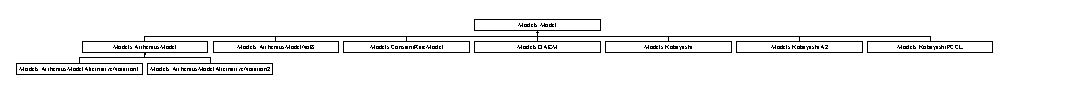
\includegraphics[height=0.777778cm]{classModels_1_1Model}
\end{center}
\end{figure}
\subsection*{\-Public \-Member \-Functions}
\begin{DoxyCompactItemize}
\item 
def \hyperlink{classModels_1_1Model_a317ed848b969dbe3a96dd05e8b771900}{plt\-Yield}
\item 
def \hyperlink{classModels_1_1Model_aa35c741babf8f141df48c4021e0664e4}{plt\-Rate}
\item 
def \hyperlink{classModels_1_1Model_a3396d6ca1a7b7d66e55ada8c3c7a509e}{max\-Length\-Of\-Vectors}
\item 
def \hyperlink{classModels_1_1Model_ae404a691e48bfe4eafcdfdd09f1dae48}{plot}
\item 
def \hyperlink{classModels_1_1Model_a010945ed2adff59a7a5fce36025e7a97}{derive\-C}
\item 
def \hyperlink{classModels_1_1Model_a7c9280e33f9e0d46703cebc131008c65}{calc\-Rate}
\item 
def \hyperlink{classModels_1_1Model_a818f207e2a4bd0e9a3720ca611960e5a}{set\-Param\-Vector}
\item 
def \hyperlink{classModels_1_1Model_a13c76a0fe24d43cdc4d21fbc73fa96fa}{\-Param\-Vector}
\item 
def \hyperlink{classModels_1_1Model_ad3e627980d9e781bf7b2c9ff900ca06b}{\-Error\-Yield}
\item 
def \hyperlink{classModels_1_1Model_a3050eb39341f318d8d88b172f88bd240}{\-Error\-Rate}
\item 
def \hyperlink{classModels_1_1Model_adcb987bccae63a742490ea1e6d5f7a74}{mk\-Simple\-Result\-Files}
\item 
def \hyperlink{classModels_1_1Model_ac28252ae5cd6b5ecd4c5d006a0e6567d}{set\-Dt4\-Intergrate}
\end{DoxyCompactItemize}
\subsection*{\-Public \-Attributes}
\begin{DoxyCompactItemize}
\item 
\hypertarget{classModels_1_1Model_aa61209c0f4ac8888bc962fee2e8d688e}{{\bfseries const\-Dt}}\label{classModels_1_1Model_aa61209c0f4ac8888bc962fee2e8d688e}

\item 
\hypertarget{classModels_1_1Model_a3f71983de5f8b86bec47929213b900ec}{{\bfseries const\-Dt\-Vec}}\label{classModels_1_1Model_a3f71983de5f8b86bec47929213b900ec}

\end{DoxyCompactItemize}


\subsection{\-Detailed \-Description}
\begin{DoxyVerb}Parent class of the children ConstantRateModel, the three Arrhenius Models (notations) and the Kobayashi models. TimeVectorToInterplt allows the option to define the discrete time points, where to interpolate the results. If set to False (standard), then is are the outputted results equal the dt to solve the ODE. If set TimeVectorToInterplt=[t0,t1,t2,t3,t4] (t: floats) then is the yields result returned at method calcMass the yields at [t0,t1,t2,t3,t4], linear interploated.\end{DoxyVerb}
 

\subsection{\-Member \-Function \-Documentation}
\hypertarget{classModels_1_1Model_a7c9280e33f9e0d46703cebc131008c65}{\index{\-Models\-::\-Model@{\-Models\-::\-Model}!calc\-Rate@{calc\-Rate}}
\index{calc\-Rate@{calc\-Rate}!Models::Model@{\-Models\-::\-Model}}
\subsubsection[{calc\-Rate}]{\setlength{\rightskip}{0pt plus 5cm}def {\bf \-Models.\-Model.\-calc\-Rate} (
\begin{DoxyParamCaption}
\item[{}]{self, }
\item[{}]{fgdvc, }
\item[{}]{time, }
\item[{}]{\-T, }
\item[{}]{\-Name}
\end{DoxyParamCaption}
)}}\label{classModels_1_1Model_a7c9280e33f9e0d46703cebc131008c65}
\begin{DoxyVerb}Generates the Rates using the yields vector and a CDS.\end{DoxyVerb}
 \hypertarget{classModels_1_1Model_a010945ed2adff59a7a5fce36025e7a97}{\index{\-Models\-::\-Model@{\-Models\-::\-Model}!derive\-C@{derive\-C}}
\index{derive\-C@{derive\-C}!Models::Model@{\-Models\-::\-Model}}
\subsubsection[{derive\-C}]{\setlength{\rightskip}{0pt plus 5cm}def {\bf \-Models.\-Model.\-derive\-C} (
\begin{DoxyParamCaption}
\item[{}]{self, }
\item[{}]{fgdvc, }
\item[{}]{y\-Vector}
\end{DoxyParamCaption}
)}}\label{classModels_1_1Model_a010945ed2adff59a7a5fce36025e7a97}
\begin{DoxyVerb}Returns a CDS of the inputted yVector.\end{DoxyVerb}
 \hypertarget{classModels_1_1Model_a3050eb39341f318d8d88b172f88bd240}{\index{\-Models\-::\-Model@{\-Models\-::\-Model}!\-Error\-Rate@{\-Error\-Rate}}
\index{\-Error\-Rate@{\-Error\-Rate}!Models::Model@{\-Models\-::\-Model}}
\subsubsection[{\-Error\-Rate}]{\setlength{\rightskip}{0pt plus 5cm}def {\bf \-Models.\-Model.\-Error\-Rate} (
\begin{DoxyParamCaption}
\item[{}]{self, }
\item[{}]{fgdvc, }
\item[{}]{\-Species}
\end{DoxyParamCaption}
)}}\label{classModels_1_1Model_a3050eb39341f318d8d88b172f88bd240}
\begin{DoxyVerb}Returns the absolute deviation per point between the fitted and the original rate curve.\end{DoxyVerb}
 \hypertarget{classModels_1_1Model_ad3e627980d9e781bf7b2c9ff900ca06b}{\index{\-Models\-::\-Model@{\-Models\-::\-Model}!\-Error\-Yield@{\-Error\-Yield}}
\index{\-Error\-Yield@{\-Error\-Yield}!Models::Model@{\-Models\-::\-Model}}
\subsubsection[{\-Error\-Yield}]{\setlength{\rightskip}{0pt plus 5cm}def {\bf \-Models.\-Model.\-Error\-Yield} (
\begin{DoxyParamCaption}
\item[{}]{self, }
\item[{}]{fgdvc, }
\item[{}]{\-Species}
\end{DoxyParamCaption}
)}}\label{classModels_1_1Model_ad3e627980d9e781bf7b2c9ff900ca06b}
\begin{DoxyVerb}Returns the absolute deviation per point between the fitted and the original yield curve.\end{DoxyVerb}
 \hypertarget{classModels_1_1Model_a3396d6ca1a7b7d66e55ada8c3c7a509e}{\index{\-Models\-::\-Model@{\-Models\-::\-Model}!max\-Length\-Of\-Vectors@{max\-Length\-Of\-Vectors}}
\index{max\-Length\-Of\-Vectors@{max\-Length\-Of\-Vectors}!Models::Model@{\-Models\-::\-Model}}
\subsubsection[{max\-Length\-Of\-Vectors}]{\setlength{\rightskip}{0pt plus 5cm}def {\bf \-Models.\-Model.\-max\-Length\-Of\-Vectors} (
\begin{DoxyParamCaption}
\item[{}]{self, }
\item[{}]{fgdvc\-\_\-list}
\end{DoxyParamCaption}
)}}\label{classModels_1_1Model_a3396d6ca1a7b7d66e55ada8c3c7a509e}
\begin{DoxyVerb}Returns the minimum lenght of a all vectors from the several runs.\end{DoxyVerb}
 \hypertarget{classModels_1_1Model_adcb987bccae63a742490ea1e6d5f7a74}{\index{\-Models\-::\-Model@{\-Models\-::\-Model}!mk\-Simple\-Result\-Files@{mk\-Simple\-Result\-Files}}
\index{mk\-Simple\-Result\-Files@{mk\-Simple\-Result\-Files}!Models::Model@{\-Models\-::\-Model}}
\subsubsection[{mk\-Simple\-Result\-Files}]{\setlength{\rightskip}{0pt plus 5cm}def {\bf \-Models.\-Model.\-mk\-Simple\-Result\-Files} (
\begin{DoxyParamCaption}
\item[{}]{self, }
\item[{}]{fgdvc\-\_\-list, }
\item[{}]{\-Species}
\end{DoxyParamCaption}
)}}\label{classModels_1_1Model_adcb987bccae63a742490ea1e6d5f7a74}
\begin{DoxyVerb}Simple result file if no fitting is carried out. Writes only the transformed results into a file.\end{DoxyVerb}
 \hypertarget{classModels_1_1Model_a13c76a0fe24d43cdc4d21fbc73fa96fa}{\index{\-Models\-::\-Model@{\-Models\-::\-Model}!\-Param\-Vector@{\-Param\-Vector}}
\index{\-Param\-Vector@{\-Param\-Vector}!Models::Model@{\-Models\-::\-Model}}
\subsubsection[{\-Param\-Vector}]{\setlength{\rightskip}{0pt plus 5cm}def {\bf \-Models.\-Model.\-Param\-Vector} (
\begin{DoxyParamCaption}
\item[{}]{self}
\end{DoxyParamCaption}
)}}\label{classModels_1_1Model_a13c76a0fe24d43cdc4d21fbc73fa96fa}
\begin{DoxyVerb}Returns the Vector containing the kinetic parameter of the Model (refering to the child model).\end{DoxyVerb}
 \hypertarget{classModels_1_1Model_ae404a691e48bfe4eafcdfdd09f1dae48}{\index{\-Models\-::\-Model@{\-Models\-::\-Model}!plot@{plot}}
\index{plot@{plot}!Models::Model@{\-Models\-::\-Model}}
\subsubsection[{plot}]{\setlength{\rightskip}{0pt plus 5cm}def {\bf \-Models.\-Model.\-plot} (
\begin{DoxyParamCaption}
\item[{}]{self, }
\item[{}]{fgdvc\-\_\-list, }
\item[{}]{\-Species}
\end{DoxyParamCaption}
)}}\label{classModels_1_1Model_ae404a691e48bfe4eafcdfdd09f1dae48}
\begin{DoxyVerb}Plot the yield and the rates over time with two curves: one is the original data, the other the fitting curve. Also file 'PyrolysisProgramName-Species.out' (e.g. 'CPD-CO2.out') containing the time (s), yields (kg/kg), rates (kg/(kg s)).\end{DoxyVerb}
 \hypertarget{classModels_1_1Model_aa35c741babf8f141df48c4021e0664e4}{\index{\-Models\-::\-Model@{\-Models\-::\-Model}!plt\-Rate@{plt\-Rate}}
\index{plt\-Rate@{plt\-Rate}!Models::Model@{\-Models\-::\-Model}}
\subsubsection[{plt\-Rate}]{\setlength{\rightskip}{0pt plus 5cm}def {\bf \-Models.\-Model.\-plt\-Rate} (
\begin{DoxyParamCaption}
\item[{}]{self, }
\item[{}]{fgdvc\-\_\-list, }
\item[{}]{x\-Value\-To\-Plot, }
\item[{}]{y\-Value\-To\-Plot}
\end{DoxyParamCaption}
)}}\label{classModels_1_1Model_aa35c741babf8f141df48c4021e0664e4}
\begin{DoxyVerb}Plots the rates (to select with yValueToPlot) over Time or Temperature (to slect with xValueToPlot).\end{DoxyVerb}
 \hypertarget{classModels_1_1Model_a317ed848b969dbe3a96dd05e8b771900}{\index{\-Models\-::\-Model@{\-Models\-::\-Model}!plt\-Yield@{plt\-Yield}}
\index{plt\-Yield@{plt\-Yield}!Models::Model@{\-Models\-::\-Model}}
\subsubsection[{plt\-Yield}]{\setlength{\rightskip}{0pt plus 5cm}def {\bf \-Models.\-Model.\-plt\-Yield} (
\begin{DoxyParamCaption}
\item[{}]{self, }
\item[{}]{fgdvc\-\_\-list, }
\item[{}]{x\-Value\-To\-Plot, }
\item[{}]{y\-Value\-To\-Plot}
\end{DoxyParamCaption}
)}}\label{classModels_1_1Model_a317ed848b969dbe3a96dd05e8b771900}
\begin{DoxyVerb}Plots the yields (to select with yValueToPlot) over Time or Temperature (to slect with xValueToPlot).\end{DoxyVerb}
 \hypertarget{classModels_1_1Model_ac28252ae5cd6b5ecd4c5d006a0e6567d}{\index{\-Models\-::\-Model@{\-Models\-::\-Model}!set\-Dt4\-Intergrate@{set\-Dt4\-Intergrate}}
\index{set\-Dt4\-Intergrate@{set\-Dt4\-Intergrate}!Models::Model@{\-Models\-::\-Model}}
\subsubsection[{set\-Dt4\-Intergrate}]{\setlength{\rightskip}{0pt plus 5cm}def {\bf \-Models.\-Model.\-set\-Dt4\-Intergrate} (
\begin{DoxyParamCaption}
\item[{}]{self, }
\item[{}]{constant\-Dt}
\end{DoxyParamCaption}
)}}\label{classModels_1_1Model_ac28252ae5cd6b5ecd4c5d006a0e6567d}
\begin{DoxyVerb}constantDt allows the option to define numerical time step to solve the ODE. The outputted results ever equal the imported time list (when applying method calcMass Time = [t0,t1,t2,t3,t4]. If these time steps are too large, then is this defined dt used to solve the ODE and the results are linear interploated that way that they correspond to the imported time vector. To reset it, just set constantDt to False.\end{DoxyVerb}
 \hypertarget{classModels_1_1Model_a818f207e2a4bd0e9a3720ca611960e5a}{\index{\-Models\-::\-Model@{\-Models\-::\-Model}!set\-Param\-Vector@{set\-Param\-Vector}}
\index{set\-Param\-Vector@{set\-Param\-Vector}!Models::Model@{\-Models\-::\-Model}}
\subsubsection[{set\-Param\-Vector}]{\setlength{\rightskip}{0pt plus 5cm}def {\bf \-Models.\-Model.\-set\-Param\-Vector} (
\begin{DoxyParamCaption}
\item[{}]{self, }
\item[{}]{\-Parameter\-List}
\end{DoxyParamCaption}
)}}\label{classModels_1_1Model_a818f207e2a4bd0e9a3720ca611960e5a}
\begin{DoxyVerb}Sets the Vector containing the kinetic parameter of the Model (refering to the child model).\end{DoxyVerb}
 

\-The documentation for this class was generated from the following file\-:\begin{DoxyCompactItemize}
\item 
/home/map/git/pkp/src/\-Models.\-py\end{DoxyCompactItemize}

\hypertarget{classFit__one__run_1_1Model}{\section{\-Fit\-\_\-one\-\_\-run.\-Model \-Class \-Reference}
\label{classFit__one__run_1_1Model}\index{\-Fit\-\_\-one\-\_\-run.\-Model@{\-Fit\-\_\-one\-\_\-run.\-Model}}
}
\-Inheritance diagram for \-Fit\-\_\-one\-\_\-run.\-Model\-:\begin{figure}[H]
\begin{center}
\leavevmode
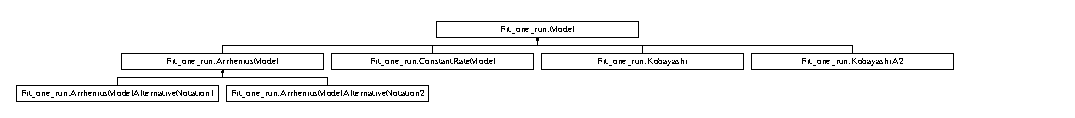
\includegraphics[height=1.131313cm]{classFit__one__run_1_1Model}
\end{center}
\end{figure}
\subsection*{\-Public \-Member \-Functions}
\begin{DoxyCompactItemize}
\item 
def \hyperlink{classFit__one__run_1_1Model_aa304b32155938a713c33f0dc03a135f3}{plt\-Yield}
\item 
def \hyperlink{classFit__one__run_1_1Model_a9c28d95902adf00f5aaa642f0919fc61}{plt\-Rate}
\item 
def \hyperlink{classFit__one__run_1_1Model_a26fc879ca33c9171ebb4a97bc4b0c46b}{min\-Length\-Of\-Vectors}
\item 
def \hyperlink{classFit__one__run_1_1Model_a98159c954f1f1be2a34be3ea53d11493}{plot}
\item 
def \hyperlink{classFit__one__run_1_1Model_ace9df4177c5ae753dbe190e2f8268149}{derive\-C}
\item 
def \hyperlink{classFit__one__run_1_1Model_a07ae4534de2a6ef241d71facdffb227e}{calc\-Rate}
\item 
def \hyperlink{classFit__one__run_1_1Model_a174aec9b05dbe01ec103f7ba75d6516c}{set\-Param\-Vector}
\item 
def \hyperlink{classFit__one__run_1_1Model_a3c9239f0ac062fdae0bda395636c0372}{\-Param\-Vector}
\item 
def \hyperlink{classFit__one__run_1_1Model_aa2bc4ba19704350fb2ff441734b51b10}{\-Error\-Yield}
\item 
def \hyperlink{classFit__one__run_1_1Model_aad63c345c343f0c7d1cf20135dc0a0e5}{\-Error\-Rate}
\end{DoxyCompactItemize}


\subsection{\-Detailed \-Description}
\begin{DoxyVerb}Parent class of the children ConstantRateModel, the three Arrhenius Models (notations) and the Kobayashi models.\end{DoxyVerb}
 

\subsection{\-Member \-Function \-Documentation}
\hypertarget{classFit__one__run_1_1Model_a07ae4534de2a6ef241d71facdffb227e}{\index{\-Fit\-\_\-one\-\_\-run\-::\-Model@{\-Fit\-\_\-one\-\_\-run\-::\-Model}!calc\-Rate@{calc\-Rate}}
\index{calc\-Rate@{calc\-Rate}!Fit_one_run::Model@{\-Fit\-\_\-one\-\_\-run\-::\-Model}}
\subsubsection[{calc\-Rate}]{\setlength{\rightskip}{0pt plus 5cm}def {\bf \-Fit\-\_\-one\-\_\-run.\-Model.\-calc\-Rate} (
\begin{DoxyParamCaption}
\item[{}]{self, }
\item[{}]{fgdvc, }
\item[{}]{time, }
\item[{}]{\-T, }
\item[{}]{\-Name}
\end{DoxyParamCaption}
)}}\label{classFit__one__run_1_1Model_a07ae4534de2a6ef241d71facdffb227e}
\begin{DoxyVerb}Generates the Rates using the yields vector and a CDS.\end{DoxyVerb}
 \hypertarget{classFit__one__run_1_1Model_ace9df4177c5ae753dbe190e2f8268149}{\index{\-Fit\-\_\-one\-\_\-run\-::\-Model@{\-Fit\-\_\-one\-\_\-run\-::\-Model}!derive\-C@{derive\-C}}
\index{derive\-C@{derive\-C}!Fit_one_run::Model@{\-Fit\-\_\-one\-\_\-run\-::\-Model}}
\subsubsection[{derive\-C}]{\setlength{\rightskip}{0pt plus 5cm}def {\bf \-Fit\-\_\-one\-\_\-run.\-Model.\-derive\-C} (
\begin{DoxyParamCaption}
\item[{}]{self, }
\item[{}]{fgdvc, }
\item[{}]{y\-Vector, }
\item[{}]{max\-Vector\-Lenght = {\ttfamily \-None}}
\end{DoxyParamCaption}
)}}\label{classFit__one__run_1_1Model_ace9df4177c5ae753dbe190e2f8268149}
\begin{DoxyVerb}Returns a CDS of the inputted yVector.\end{DoxyVerb}
 \hypertarget{classFit__one__run_1_1Model_aad63c345c343f0c7d1cf20135dc0a0e5}{\index{\-Fit\-\_\-one\-\_\-run\-::\-Model@{\-Fit\-\_\-one\-\_\-run\-::\-Model}!\-Error\-Rate@{\-Error\-Rate}}
\index{\-Error\-Rate@{\-Error\-Rate}!Fit_one_run::Model@{\-Fit\-\_\-one\-\_\-run\-::\-Model}}
\subsubsection[{\-Error\-Rate}]{\setlength{\rightskip}{0pt plus 5cm}def {\bf \-Fit\-\_\-one\-\_\-run.\-Model.\-Error\-Rate} (
\begin{DoxyParamCaption}
\item[{}]{self, }
\item[{}]{fgdvc, }
\item[{}]{\-Species}
\end{DoxyParamCaption}
)}}\label{classFit__one__run_1_1Model_aad63c345c343f0c7d1cf20135dc0a0e5}
\begin{DoxyVerb}Returns the absolute deviation per point between the fitted and the original rate curve.\end{DoxyVerb}
 \hypertarget{classFit__one__run_1_1Model_aa2bc4ba19704350fb2ff441734b51b10}{\index{\-Fit\-\_\-one\-\_\-run\-::\-Model@{\-Fit\-\_\-one\-\_\-run\-::\-Model}!\-Error\-Yield@{\-Error\-Yield}}
\index{\-Error\-Yield@{\-Error\-Yield}!Fit_one_run::Model@{\-Fit\-\_\-one\-\_\-run\-::\-Model}}
\subsubsection[{\-Error\-Yield}]{\setlength{\rightskip}{0pt plus 5cm}def {\bf \-Fit\-\_\-one\-\_\-run.\-Model.\-Error\-Yield} (
\begin{DoxyParamCaption}
\item[{}]{self, }
\item[{}]{fgdvc, }
\item[{}]{\-Species}
\end{DoxyParamCaption}
)}}\label{classFit__one__run_1_1Model_aa2bc4ba19704350fb2ff441734b51b10}
\begin{DoxyVerb}Returns the absolute deviation per point between the fitted and the original yield curve.\end{DoxyVerb}
 \hypertarget{classFit__one__run_1_1Model_a26fc879ca33c9171ebb4a97bc4b0c46b}{\index{\-Fit\-\_\-one\-\_\-run\-::\-Model@{\-Fit\-\_\-one\-\_\-run\-::\-Model}!min\-Length\-Of\-Vectors@{min\-Length\-Of\-Vectors}}
\index{min\-Length\-Of\-Vectors@{min\-Length\-Of\-Vectors}!Fit_one_run::Model@{\-Fit\-\_\-one\-\_\-run\-::\-Model}}
\subsubsection[{min\-Length\-Of\-Vectors}]{\setlength{\rightskip}{0pt plus 5cm}def {\bf \-Fit\-\_\-one\-\_\-run.\-Model.\-min\-Length\-Of\-Vectors} (
\begin{DoxyParamCaption}
\item[{}]{self, }
\item[{}]{fgdvc\-\_\-list}
\end{DoxyParamCaption}
)}}\label{classFit__one__run_1_1Model_a26fc879ca33c9171ebb4a97bc4b0c46b}
\begin{DoxyVerb}Returns the minimum lenght of a all vectors from the several runs.\end{DoxyVerb}
 \hypertarget{classFit__one__run_1_1Model_a3c9239f0ac062fdae0bda395636c0372}{\index{\-Fit\-\_\-one\-\_\-run\-::\-Model@{\-Fit\-\_\-one\-\_\-run\-::\-Model}!\-Param\-Vector@{\-Param\-Vector}}
\index{\-Param\-Vector@{\-Param\-Vector}!Fit_one_run::Model@{\-Fit\-\_\-one\-\_\-run\-::\-Model}}
\subsubsection[{\-Param\-Vector}]{\setlength{\rightskip}{0pt plus 5cm}def {\bf \-Fit\-\_\-one\-\_\-run.\-Model.\-Param\-Vector} (
\begin{DoxyParamCaption}
\item[{}]{self}
\end{DoxyParamCaption}
)}}\label{classFit__one__run_1_1Model_a3c9239f0ac062fdae0bda395636c0372}
\begin{DoxyVerb}Returns the Vector containing the kinetic parameter of the Model (refering to the child model).\end{DoxyVerb}
 \hypertarget{classFit__one__run_1_1Model_a98159c954f1f1be2a34be3ea53d11493}{\index{\-Fit\-\_\-one\-\_\-run\-::\-Model@{\-Fit\-\_\-one\-\_\-run\-::\-Model}!plot@{plot}}
\index{plot@{plot}!Fit_one_run::Model@{\-Fit\-\_\-one\-\_\-run\-::\-Model}}
\subsubsection[{plot}]{\setlength{\rightskip}{0pt plus 5cm}def {\bf \-Fit\-\_\-one\-\_\-run.\-Model.\-plot} (
\begin{DoxyParamCaption}
\item[{}]{self, }
\item[{}]{fgdvc\-\_\-list, }
\item[{}]{\-Species}
\end{DoxyParamCaption}
)}}\label{classFit__one__run_1_1Model_a98159c954f1f1be2a34be3ea53d11493}
\begin{DoxyVerb}Plot the yield and the rates over time with two curves: one is the original data, the other the fitting curve. Also file 'PyrolysisProgramName-Species.out' (e.g. 'CPD-CO2.out') containing the time (s), yields (kg/kg), rates (kg/(kg s)).\end{DoxyVerb}
 \hypertarget{classFit__one__run_1_1Model_a9c28d95902adf00f5aaa642f0919fc61}{\index{\-Fit\-\_\-one\-\_\-run\-::\-Model@{\-Fit\-\_\-one\-\_\-run\-::\-Model}!plt\-Rate@{plt\-Rate}}
\index{plt\-Rate@{plt\-Rate}!Fit_one_run::Model@{\-Fit\-\_\-one\-\_\-run\-::\-Model}}
\subsubsection[{plt\-Rate}]{\setlength{\rightskip}{0pt plus 5cm}def {\bf \-Fit\-\_\-one\-\_\-run.\-Model.\-plt\-Rate} (
\begin{DoxyParamCaption}
\item[{}]{self, }
\item[{}]{fgdvc\-\_\-list, }
\item[{}]{x\-Value\-To\-Plot, }
\item[{}]{y\-Value\-To\-Plot}
\end{DoxyParamCaption}
)}}\label{classFit__one__run_1_1Model_a9c28d95902adf00f5aaa642f0919fc61}
\begin{DoxyVerb}Plots the rates (to select with yValueToPlot) over Time or Temperature (to slect with xValueToPlot).\end{DoxyVerb}
 \hypertarget{classFit__one__run_1_1Model_aa304b32155938a713c33f0dc03a135f3}{\index{\-Fit\-\_\-one\-\_\-run\-::\-Model@{\-Fit\-\_\-one\-\_\-run\-::\-Model}!plt\-Yield@{plt\-Yield}}
\index{plt\-Yield@{plt\-Yield}!Fit_one_run::Model@{\-Fit\-\_\-one\-\_\-run\-::\-Model}}
\subsubsection[{plt\-Yield}]{\setlength{\rightskip}{0pt plus 5cm}def {\bf \-Fit\-\_\-one\-\_\-run.\-Model.\-plt\-Yield} (
\begin{DoxyParamCaption}
\item[{}]{self, }
\item[{}]{fgdvc\-\_\-list, }
\item[{}]{x\-Value\-To\-Plot, }
\item[{}]{y\-Value\-To\-Plot}
\end{DoxyParamCaption}
)}}\label{classFit__one__run_1_1Model_aa304b32155938a713c33f0dc03a135f3}
\begin{DoxyVerb}Plots the yields (to select with yValueToPlot) over Time or Temperature (to slect with xValueToPlot).\end{DoxyVerb}
 \hypertarget{classFit__one__run_1_1Model_a174aec9b05dbe01ec103f7ba75d6516c}{\index{\-Fit\-\_\-one\-\_\-run\-::\-Model@{\-Fit\-\_\-one\-\_\-run\-::\-Model}!set\-Param\-Vector@{set\-Param\-Vector}}
\index{set\-Param\-Vector@{set\-Param\-Vector}!Fit_one_run::Model@{\-Fit\-\_\-one\-\_\-run\-::\-Model}}
\subsubsection[{set\-Param\-Vector}]{\setlength{\rightskip}{0pt plus 5cm}def {\bf \-Fit\-\_\-one\-\_\-run.\-Model.\-set\-Param\-Vector} (
\begin{DoxyParamCaption}
\item[{}]{self, }
\item[{}]{\-Parameter\-List}
\end{DoxyParamCaption}
)}}\label{classFit__one__run_1_1Model_a174aec9b05dbe01ec103f7ba75d6516c}
\begin{DoxyVerb}Sets the Vector containing the kinetic parameter of the Model (refering to the child model).\end{DoxyVerb}
 

\-The documentation for this class was generated from the following file\-:\begin{DoxyCompactItemize}
\item 
/home/map/git/pkp/src/\-Fit\-\_\-one\-\_\-run.\-py\end{DoxyCompactItemize}

\hypertarget{classmatplotlibwidgetFile_1_1MplCanvas}{\section{matplotlibwidget\-File.\-Mpl\-Canvas \-Class \-Reference}
\label{classmatplotlibwidgetFile_1_1MplCanvas}\index{matplotlibwidget\-File.\-Mpl\-Canvas@{matplotlibwidget\-File.\-Mpl\-Canvas}}
}
\subsection*{\-Public \-Member \-Functions}
\begin{DoxyCompactItemize}
\item 
\hypertarget{classmatplotlibwidgetFile_1_1MplCanvas_a6eb3342e3b3e6a6d49385be5456f6ad9}{def {\bfseries \-\_\-\-\_\-init\-\_\-\-\_\-}}\label{classmatplotlibwidgetFile_1_1MplCanvas_a6eb3342e3b3e6a6d49385be5456f6ad9}

\end{DoxyCompactItemize}
\subsection*{\-Public \-Attributes}
\begin{DoxyCompactItemize}
\item 
\hypertarget{classmatplotlibwidgetFile_1_1MplCanvas_ac2706b697b985cc1b16feaa545b1c4f9}{{\bfseries fig}}\label{classmatplotlibwidgetFile_1_1MplCanvas_ac2706b697b985cc1b16feaa545b1c4f9}

\item 
\hypertarget{classmatplotlibwidgetFile_1_1MplCanvas_aff43023ca9dd98716cee5616643e8d55}{{\bfseries ax}}\label{classmatplotlibwidgetFile_1_1MplCanvas_aff43023ca9dd98716cee5616643e8d55}

\end{DoxyCompactItemize}


\-The documentation for this class was generated from the following file\-:\begin{DoxyCompactItemize}
\item 
/home/map/git/pkp/src/matplotlibwidget\-File.\-py\end{DoxyCompactItemize}

\hypertarget{classInformationFiles_1_1OperCondInput}{\section{\-Information\-Files.\-Oper\-Cond\-Input \-Class \-Reference}
\label{classInformationFiles_1_1OperCondInput}\index{\-Information\-Files.\-Oper\-Cond\-Input@{\-Information\-Files.\-Oper\-Cond\-Input}}
}
\-Inheritance diagram for \-Information\-Files.\-Oper\-Cond\-Input\-:\begin{figure}[H]
\begin{center}
\leavevmode
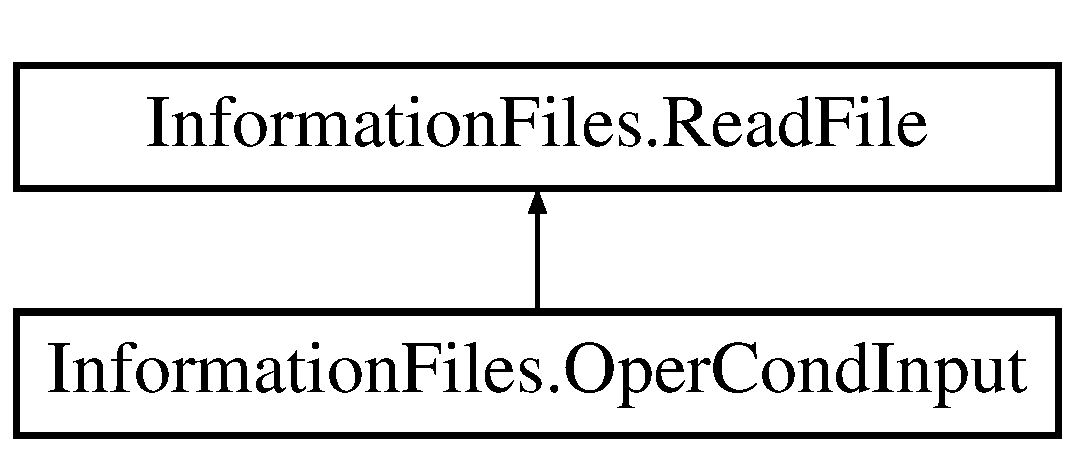
\includegraphics[height=2.000000cm]{classInformationFiles_1_1OperCondInput}
\end{center}
\end{figure}
\subsection*{\-Public \-Member \-Functions}
\begin{DoxyCompactItemize}
\item 
\hypertarget{classInformationFiles_1_1OperCondInput_af0db75c31c93a384cd7c83ee3283e8cf}{def {\bfseries \-\_\-\-\_\-init\-\_\-\-\_\-}}\label{classInformationFiles_1_1OperCondInput_af0db75c31c93a384cd7c83ee3283e8cf}

\item 
def \hyperlink{classInformationFiles_1_1OperCondInput_a993543ba04b3cda447a87931d1fef3ee}{get\-Time\-Points}
\item 
def \hyperlink{classInformationFiles_1_1OperCondInput_a57778c39c852ab2677846881031db6fc}{write\-F\-G\-D\-V\-Ct\-T\-Hist}
\item 
\hypertarget{classInformationFiles_1_1OperCondInput_ae4daea252d62f9d057c314f3bbddbb37}{def {\bfseries \-Number\-Of\-Lines}}\label{classInformationFiles_1_1OperCondInput_ae4daea252d62f9d057c314f3bbddbb37}

\item 
def \hyperlink{classInformationFiles_1_1ReadFile_a33eb756d9e63ef0f7e0ad1c175406ef0}{read\-Lines}
\item 
def \hyperlink{classInformationFiles_1_1ReadFile_a259b8dd2f0754fe46c67e1af6c82ec5d}{\-Use\-Pyrol\-Progr}
\item 
def \hyperlink{classInformationFiles_1_1ReadFile_acbbf6f298c76c66d18d56c787225fcb7}{\-Fitting}
\item 
def \hyperlink{classInformationFiles_1_1ReadFile_a2911cbdb92a645b6114feca74fc69aba}{get\-Value}
\item 
def \hyperlink{classInformationFiles_1_1ReadFile_ae3432e04c7dde26bbcdb97d4436c1d70}{get\-Text}
\end{DoxyCompactItemize}
\subsection*{\-Public \-Attributes}
\begin{DoxyCompactItemize}
\item 
\hypertarget{classInformationFiles_1_1OperCondInput_adeaba3436443e37d67a422b2e567c0a9}{{\bfseries \-Input\-File}}\label{classInformationFiles_1_1OperCondInput_adeaba3436443e37d67a422b2e567c0a9}

\item 
\hypertarget{classInformationFiles_1_1OperCondInput_ab57a754cfdf444860a808eb0dc149691}{{\bfseries \-Input}}\label{classInformationFiles_1_1OperCondInput_ab57a754cfdf444860a808eb0dc149691}

\end{DoxyCompactItemize}
\subsection*{\-Static \-Public \-Attributes}
\begin{DoxyCompactItemize}
\item 
\hypertarget{classInformationFiles_1_1OperCondInput_a5a172e0266c4c4940cba6147b66c84cf}{tuple {\bfseries \-Time\-Temp} = np.\-genfromtxt(self.\-Input\mbox{[}\-Begin\-Line\-:\-End\-Line\mbox{]}, delimiter=',')}\label{classInformationFiles_1_1OperCondInput_a5a172e0266c4c4940cba6147b66c84cf}

\end{DoxyCompactItemize}


\subsection{\-Detailed \-Description}
\begin{DoxyVerb}Reads the input file for the operating conditions and also writes the temperature-history file, required by FG-DVC.\end{DoxyVerb}
 

\subsection{\-Member \-Function \-Documentation}
\hypertarget{classInformationFiles_1_1ReadFile_acbbf6f298c76c66d18d56c787225fcb7}{\index{\-Information\-Files\-::\-Oper\-Cond\-Input@{\-Information\-Files\-::\-Oper\-Cond\-Input}!\-Fitting@{\-Fitting}}
\index{\-Fitting@{\-Fitting}!InformationFiles::OperCondInput@{\-Information\-Files\-::\-Oper\-Cond\-Input}}
\subsubsection[{\-Fitting}]{\setlength{\rightskip}{0pt plus 5cm}def {\bf \-Information\-Files.\-Read\-File.\-Fitting} (
\begin{DoxyParamCaption}
\item[{}]{self, }
\item[{}]{\-File\-Note}
\end{DoxyParamCaption}
)\hspace{0.3cm}{\ttfamily  \mbox{[}inherited\mbox{]}}}}\label{classInformationFiles_1_1ReadFile_acbbf6f298c76c66d18d56c787225fcb7}
\begin{DoxyVerb}outputs the Fitting mode for Pyrolysis Program output (string: 'constantRate','Arrhenius','Kobayashi'). Possible input: 'constantRate', 'Arrhenius' or 'Kobayashi'\end{DoxyVerb}
 \hypertarget{classInformationFiles_1_1ReadFile_ae3432e04c7dde26bbcdb97d4436c1d70}{\index{\-Information\-Files\-::\-Oper\-Cond\-Input@{\-Information\-Files\-::\-Oper\-Cond\-Input}!get\-Text@{get\-Text}}
\index{get\-Text@{get\-Text}!InformationFiles::OperCondInput@{\-Information\-Files\-::\-Oper\-Cond\-Input}}
\subsubsection[{get\-Text}]{\setlength{\rightskip}{0pt plus 5cm}def {\bf \-Information\-Files.\-Read\-File.\-get\-Text} (
\begin{DoxyParamCaption}
\item[{}]{self, }
\item[{}]{\-File\-Note}
\end{DoxyParamCaption}
)\hspace{0.3cm}{\ttfamily  \mbox{[}inherited\mbox{]}}}}\label{classInformationFiles_1_1ReadFile_ae3432e04c7dde26bbcdb97d4436c1d70}
\begin{DoxyVerb}output the data of the line below the FileNote as a string\end{DoxyVerb}
 \hypertarget{classInformationFiles_1_1OperCondInput_a993543ba04b3cda447a87931d1fef3ee}{\index{\-Information\-Files\-::\-Oper\-Cond\-Input@{\-Information\-Files\-::\-Oper\-Cond\-Input}!get\-Time\-Points@{get\-Time\-Points}}
\index{get\-Time\-Points@{get\-Time\-Points}!InformationFiles::OperCondInput@{\-Information\-Files\-::\-Oper\-Cond\-Input}}
\subsubsection[{get\-Time\-Points}]{\setlength{\rightskip}{0pt plus 5cm}def {\bf \-Information\-Files.\-Oper\-Cond\-Input.\-get\-Time\-Points} (
\begin{DoxyParamCaption}
\item[{}]{self, }
\item[{}]{\-File\-Note\-Begin, }
\item[{}]{\-File\-Note\-End}
\end{DoxyParamCaption}
)}}\label{classInformationFiles_1_1OperCondInput_a993543ba04b3cda447a87931d1fef3ee}
\begin{DoxyVerb}reads the time points in the shape 'time, temperature' for the lines between the line with the FileNoteBegin and the line with the FileNoteEnd\end{DoxyVerb}
 \hypertarget{classInformationFiles_1_1ReadFile_a2911cbdb92a645b6114feca74fc69aba}{\index{\-Information\-Files\-::\-Oper\-Cond\-Input@{\-Information\-Files\-::\-Oper\-Cond\-Input}!get\-Value@{get\-Value}}
\index{get\-Value@{get\-Value}!InformationFiles::OperCondInput@{\-Information\-Files\-::\-Oper\-Cond\-Input}}
\subsubsection[{get\-Value}]{\setlength{\rightskip}{0pt plus 5cm}def {\bf \-Information\-Files.\-Read\-File.\-get\-Value} (
\begin{DoxyParamCaption}
\item[{}]{self, }
\item[{}]{\-File\-Note}
\end{DoxyParamCaption}
)\hspace{0.3cm}{\ttfamily  \mbox{[}inherited\mbox{]}}}}\label{classInformationFiles_1_1ReadFile_a2911cbdb92a645b6114feca74fc69aba}
\begin{DoxyVerb}output the data of the line below the FileNote as a float\end{DoxyVerb}
 \hypertarget{classInformationFiles_1_1ReadFile_a33eb756d9e63ef0f7e0ad1c175406ef0}{\index{\-Information\-Files\-::\-Oper\-Cond\-Input@{\-Information\-Files\-::\-Oper\-Cond\-Input}!read\-Lines@{read\-Lines}}
\index{read\-Lines@{read\-Lines}!InformationFiles::OperCondInput@{\-Information\-Files\-::\-Oper\-Cond\-Input}}
\subsubsection[{read\-Lines}]{\setlength{\rightskip}{0pt plus 5cm}def {\bf \-Information\-Files.\-Read\-File.\-read\-Lines} (
\begin{DoxyParamCaption}
\item[{}]{self}
\end{DoxyParamCaption}
)\hspace{0.3cm}{\ttfamily  \mbox{[}inherited\mbox{]}}}}\label{classInformationFiles_1_1ReadFile_a33eb756d9e63ef0f7e0ad1c175406ef0}
\begin{DoxyVerb}reads the input File line by line\end{DoxyVerb}
 \hypertarget{classInformationFiles_1_1ReadFile_a259b8dd2f0754fe46c67e1af6c82ec5d}{\index{\-Information\-Files\-::\-Oper\-Cond\-Input@{\-Information\-Files\-::\-Oper\-Cond\-Input}!\-Use\-Pyrol\-Progr@{\-Use\-Pyrol\-Progr}}
\index{\-Use\-Pyrol\-Progr@{\-Use\-Pyrol\-Progr}!InformationFiles::OperCondInput@{\-Information\-Files\-::\-Oper\-Cond\-Input}}
\subsubsection[{\-Use\-Pyrol\-Progr}]{\setlength{\rightskip}{0pt plus 5cm}def {\bf \-Information\-Files.\-Read\-File.\-Use\-Pyrol\-Progr} (
\begin{DoxyParamCaption}
\item[{}]{self, }
\item[{}]{\-File\-Note}
\end{DoxyParamCaption}
)\hspace{0.3cm}{\ttfamily  \mbox{[}inherited\mbox{]}}}}\label{classInformationFiles_1_1ReadFile_a259b8dd2f0754fe46c67e1af6c82ec5d}
\begin{DoxyVerb}gets the information, whether Pyrolsis Program will be in use. Enter 'Yes' or 'True' for the case it should be used\end{DoxyVerb}
 \hypertarget{classInformationFiles_1_1OperCondInput_a57778c39c852ab2677846881031db6fc}{\index{\-Information\-Files\-::\-Oper\-Cond\-Input@{\-Information\-Files\-::\-Oper\-Cond\-Input}!write\-F\-G\-D\-V\-Ct\-T\-Hist@{write\-F\-G\-D\-V\-Ct\-T\-Hist}}
\index{write\-F\-G\-D\-V\-Ct\-T\-Hist@{write\-F\-G\-D\-V\-Ct\-T\-Hist}!InformationFiles::OperCondInput@{\-Information\-Files\-::\-Oper\-Cond\-Input}}
\subsubsection[{write\-F\-G\-D\-V\-Ct\-T\-Hist}]{\setlength{\rightskip}{0pt plus 5cm}def {\bf \-Information\-Files.\-Oper\-Cond\-Input.\-write\-F\-G\-D\-V\-Ct\-T\-Hist} (
\begin{DoxyParamCaption}
\item[{}]{self, }
\item[{}]{t\-T\-Points, }
\item[{}]{dt, }
\item[{}]{\-Output\-File\-Path}
\end{DoxyParamCaption}
)}}\label{classInformationFiles_1_1OperCondInput_a57778c39c852ab2677846881031db6fc}
\begin{DoxyVerb}Writes output file for FG-DVC containing in first column time in s, in the second tempearure in degree Celsius. FG-DVC will import this file. The time-temperature array has to be a numpy.array, dt a float, OutputFilePath a string.\end{DoxyVerb}
 

\-The documentation for this class was generated from the following file\-:\begin{DoxyCompactItemize}
\item 
/home/map/git/pkp/src/\-Information\-Files.\-py\end{DoxyCompactItemize}

\hypertarget{classPCCL__Result_1_1PCCL__Result}{\section{\-P\-C\-C\-L\-\_\-\-Result.\-P\-C\-C\-L\-\_\-\-Result \-Class \-Reference}
\label{classPCCL__Result_1_1PCCL__Result}\index{\-P\-C\-C\-L\-\_\-\-Result.\-P\-C\-C\-L\-\_\-\-Result@{\-P\-C\-C\-L\-\_\-\-Result.\-P\-C\-C\-L\-\_\-\-Result}}
}
\subsection*{\-Public \-Member \-Functions}
\begin{DoxyCompactItemize}
\item 
\hypertarget{classPCCL__Result_1_1PCCL__Result_af3390b5f925964d5227a969d577efe32}{def {\bfseries \-\_\-\-\_\-init\-\_\-\-\_\-}}\label{classPCCL__Result_1_1PCCL__Result_af3390b5f925964d5227a969d577efe32}

\item 
def \hyperlink{classPCCL__Result_1_1PCCL__Result_a199c995af0719c0500a23e7092df6ad1}{\-Yields\-\_\-all}
\item 
def \hyperlink{classPCCL__Result_1_1PCCL__Result_a04fd246373c3dfa3360826416cfcdaae}{\-Rates\-\_\-all}
\item 
def \hyperlink{classPCCL__Result_1_1PCCL__Result_a1db7606bece3c3b78ae23ba23dca2a0b}{\-Dict\-Yields2\-Cols}
\item 
def \hyperlink{classPCCL__Result_1_1PCCL__Result_a64cf9033caccee7800ba4df915ba97e8}{\-Dict\-Cols2\-Yields}
\item 
def \hyperlink{classPCCL__Result_1_1PCCL__Result_a79e44dfa48b5a07b45c5b70ba75807df}{\-Final\-Yields}
\item 
def \hyperlink{classPCCL__Result_1_1PCCL__Result_aea2be91d16bbd012e000f6534001f633}{\-File\-Path}
\item 
def \hyperlink{classPCCL__Result_1_1PCCL__Result_a6df191b5655ab7926ac1bfb550cbb317}{\-Name}
\end{DoxyCompactItemize}
\subsection*{\-Public \-Attributes}
\begin{DoxyCompactItemize}
\item 
\hypertarget{classPCCL__Result_1_1PCCL__Result_af2b6c67c8b38b1c0f856f96a003d9142}{{\bfseries \-Yields2\-Cols}}\label{classPCCL__Result_1_1PCCL__Result_af2b6c67c8b38b1c0f856f96a003d9142}

\item 
\hypertarget{classPCCL__Result_1_1PCCL__Result_a0ae6f5e4da70a7caf2470b350b9a91cc}{{\bfseries \-Cols2\-Yields}}\label{classPCCL__Result_1_1PCCL__Result_a0ae6f5e4da70a7caf2470b350b9a91cc}

\end{DoxyCompactItemize}


\subsection{\-Detailed \-Description}
\begin{DoxyVerb}Reads the PC Coal Lab input and saves the values in one array. The results include the yields of the species. The rates for all species are calculated using a CDS. This class also contains the dictionaries for the columns in the array - the name of the species. These dictionaries might be PC Coal Lab - Version dependent and the only thing which has to be changed for the case of a new release of FG-DVC with a new order of species in the result files (this was made for Version 4.1).\end{DoxyVerb}
 

\subsection{\-Member \-Function \-Documentation}
\hypertarget{classPCCL__Result_1_1PCCL__Result_a64cf9033caccee7800ba4df915ba97e8}{\index{\-P\-C\-C\-L\-\_\-\-Result\-::\-P\-C\-C\-L\-\_\-\-Result@{\-P\-C\-C\-L\-\_\-\-Result\-::\-P\-C\-C\-L\-\_\-\-Result}!\-Dict\-Cols2\-Yields@{\-Dict\-Cols2\-Yields}}
\index{\-Dict\-Cols2\-Yields@{\-Dict\-Cols2\-Yields}!PCCL_Result::PCCL_Result@{\-P\-C\-C\-L\-\_\-\-Result\-::\-P\-C\-C\-L\-\_\-\-Result}}
\subsubsection[{\-Dict\-Cols2\-Yields}]{\setlength{\rightskip}{0pt plus 5cm}def {\bf \-P\-C\-C\-L\-\_\-\-Result.\-P\-C\-C\-L\-\_\-\-Result.\-Dict\-Cols2\-Yields} (
\begin{DoxyParamCaption}
\item[{}]{self}
\end{DoxyParamCaption}
)}}\label{classPCCL__Result_1_1PCCL__Result_a64cf9033caccee7800ba4df915ba97e8}
\begin{DoxyVerb}Returns the whole Dictionary Columns of the matrix to Yield names\end{DoxyVerb}
 \hypertarget{classPCCL__Result_1_1PCCL__Result_a1db7606bece3c3b78ae23ba23dca2a0b}{\index{\-P\-C\-C\-L\-\_\-\-Result\-::\-P\-C\-C\-L\-\_\-\-Result@{\-P\-C\-C\-L\-\_\-\-Result\-::\-P\-C\-C\-L\-\_\-\-Result}!\-Dict\-Yields2\-Cols@{\-Dict\-Yields2\-Cols}}
\index{\-Dict\-Yields2\-Cols@{\-Dict\-Yields2\-Cols}!PCCL_Result::PCCL_Result@{\-P\-C\-C\-L\-\_\-\-Result\-::\-P\-C\-C\-L\-\_\-\-Result}}
\subsubsection[{\-Dict\-Yields2\-Cols}]{\setlength{\rightskip}{0pt plus 5cm}def {\bf \-P\-C\-C\-L\-\_\-\-Result.\-P\-C\-C\-L\-\_\-\-Result.\-Dict\-Yields2\-Cols} (
\begin{DoxyParamCaption}
\item[{}]{self}
\end{DoxyParamCaption}
)}}\label{classPCCL__Result_1_1PCCL__Result_a1db7606bece3c3b78ae23ba23dca2a0b}
\begin{DoxyVerb}Returns the whole Dictionary Yield names to Columns of the matrix\end{DoxyVerb}
 \hypertarget{classPCCL__Result_1_1PCCL__Result_aea2be91d16bbd012e000f6534001f633}{\index{\-P\-C\-C\-L\-\_\-\-Result\-::\-P\-C\-C\-L\-\_\-\-Result@{\-P\-C\-C\-L\-\_\-\-Result\-::\-P\-C\-C\-L\-\_\-\-Result}!\-File\-Path@{\-File\-Path}}
\index{\-File\-Path@{\-File\-Path}!PCCL_Result::PCCL_Result@{\-P\-C\-C\-L\-\_\-\-Result\-::\-P\-C\-C\-L\-\_\-\-Result}}
\subsubsection[{\-File\-Path}]{\setlength{\rightskip}{0pt plus 5cm}def {\bf \-P\-C\-C\-L\-\_\-\-Result.\-P\-C\-C\-L\-\_\-\-Result.\-File\-Path} (
\begin{DoxyParamCaption}
\item[{}]{self}
\end{DoxyParamCaption}
)}}\label{classPCCL__Result_1_1PCCL__Result_aea2be91d16bbd012e000f6534001f633}
\begin{DoxyVerb}Returns the FG-DVC File path\end{DoxyVerb}
 \hypertarget{classPCCL__Result_1_1PCCL__Result_a79e44dfa48b5a07b45c5b70ba75807df}{\index{\-P\-C\-C\-L\-\_\-\-Result\-::\-P\-C\-C\-L\-\_\-\-Result@{\-P\-C\-C\-L\-\_\-\-Result\-::\-P\-C\-C\-L\-\_\-\-Result}!\-Final\-Yields@{\-Final\-Yields}}
\index{\-Final\-Yields@{\-Final\-Yields}!PCCL_Result::PCCL_Result@{\-P\-C\-C\-L\-\_\-\-Result\-::\-P\-C\-C\-L\-\_\-\-Result}}
\subsubsection[{\-Final\-Yields}]{\setlength{\rightskip}{0pt plus 5cm}def {\bf \-P\-C\-C\-L\-\_\-\-Result.\-P\-C\-C\-L\-\_\-\-Result.\-Final\-Yields} (
\begin{DoxyParamCaption}
\item[{}]{self}
\end{DoxyParamCaption}
)}}\label{classPCCL__Result_1_1PCCL__Result_a79e44dfa48b5a07b45c5b70ba75807df}
\begin{DoxyVerb}Returns the last line of the Array, containing the yields at the time=time_End\end{DoxyVerb}
 \hypertarget{classPCCL__Result_1_1PCCL__Result_a6df191b5655ab7926ac1bfb550cbb317}{\index{\-P\-C\-C\-L\-\_\-\-Result\-::\-P\-C\-C\-L\-\_\-\-Result@{\-P\-C\-C\-L\-\_\-\-Result\-::\-P\-C\-C\-L\-\_\-\-Result}!\-Name@{\-Name}}
\index{\-Name@{\-Name}!PCCL_Result::PCCL_Result@{\-P\-C\-C\-L\-\_\-\-Result\-::\-P\-C\-C\-L\-\_\-\-Result}}
\subsubsection[{\-Name}]{\setlength{\rightskip}{0pt plus 5cm}def {\bf \-P\-C\-C\-L\-\_\-\-Result.\-P\-C\-C\-L\-\_\-\-Result.\-Name} (
\begin{DoxyParamCaption}
\item[{}]{self}
\end{DoxyParamCaption}
)}}\label{classPCCL__Result_1_1PCCL__Result_a6df191b5655ab7926ac1bfb550cbb317}
\begin{DoxyVerb}returns 'FG-DVC' as the name of the Program\end{DoxyVerb}
 \hypertarget{classPCCL__Result_1_1PCCL__Result_a04fd246373c3dfa3360826416cfcdaae}{\index{\-P\-C\-C\-L\-\_\-\-Result\-::\-P\-C\-C\-L\-\_\-\-Result@{\-P\-C\-C\-L\-\_\-\-Result\-::\-P\-C\-C\-L\-\_\-\-Result}!\-Rates\-\_\-all@{\-Rates\-\_\-all}}
\index{\-Rates\-\_\-all@{\-Rates\-\_\-all}!PCCL_Result::PCCL_Result@{\-P\-C\-C\-L\-\_\-\-Result\-::\-P\-C\-C\-L\-\_\-\-Result}}
\subsubsection[{\-Rates\-\_\-all}]{\setlength{\rightskip}{0pt plus 5cm}def {\bf \-P\-C\-C\-L\-\_\-\-Result.\-P\-C\-C\-L\-\_\-\-Result.\-Rates\-\_\-all} (
\begin{DoxyParamCaption}
\item[{}]{self}
\end{DoxyParamCaption}
)}}\label{classPCCL__Result_1_1PCCL__Result_a04fd246373c3dfa3360826416cfcdaae}
\begin{DoxyVerb}Returns the whole result matrix of the Rates.\end{DoxyVerb}
 \hypertarget{classPCCL__Result_1_1PCCL__Result_a199c995af0719c0500a23e7092df6ad1}{\index{\-P\-C\-C\-L\-\_\-\-Result\-::\-P\-C\-C\-L\-\_\-\-Result@{\-P\-C\-C\-L\-\_\-\-Result\-::\-P\-C\-C\-L\-\_\-\-Result}!\-Yields\-\_\-all@{\-Yields\-\_\-all}}
\index{\-Yields\-\_\-all@{\-Yields\-\_\-all}!PCCL_Result::PCCL_Result@{\-P\-C\-C\-L\-\_\-\-Result\-::\-P\-C\-C\-L\-\_\-\-Result}}
\subsubsection[{\-Yields\-\_\-all}]{\setlength{\rightskip}{0pt plus 5cm}def {\bf \-P\-C\-C\-L\-\_\-\-Result.\-P\-C\-C\-L\-\_\-\-Result.\-Yields\-\_\-all} (
\begin{DoxyParamCaption}
\item[{}]{self}
\end{DoxyParamCaption}
)}}\label{classPCCL__Result_1_1PCCL__Result_a199c995af0719c0500a23e7092df6ad1}
\begin{DoxyVerb}Returns the whole result matrix of the yields.\end{DoxyVerb}
 

\-The documentation for this class was generated from the following file\-:\begin{DoxyCompactItemize}
\item 
/home/map/git/pkp/src/\-P\-C\-C\-L\-\_\-\-Result.\-py\end{DoxyCompactItemize}

\hypertarget{classFGDVC__SetAndLaunch_1_1Process}{\section{\-F\-G\-D\-V\-C\-\_\-\-Set\-And\-Launch.\-Process \-Class \-Reference}
\label{classFGDVC__SetAndLaunch_1_1Process}\index{\-F\-G\-D\-V\-C\-\_\-\-Set\-And\-Launch.\-Process@{\-F\-G\-D\-V\-C\-\_\-\-Set\-And\-Launch.\-Process}}
}


\-The documentation for this class was generated from the following file\-:\begin{DoxyCompactItemize}
\item 
/home/map/git/pkp/src/\-F\-G\-D\-V\-C\-\_\-\-Set\-And\-Launch.\-py\end{DoxyCompactItemize}

\hypertarget{classCPD__SetAndLaunch_1_1ProcessCPD}{\section{\-C\-P\-D\-\_\-\-Set\-And\-Launch.\-Process\-C\-P\-D \-Class \-Reference}
\label{classCPD__SetAndLaunch_1_1ProcessCPD}\index{\-C\-P\-D\-\_\-\-Set\-And\-Launch.\-Process\-C\-P\-D@{\-C\-P\-D\-\_\-\-Set\-And\-Launch.\-Process\-C\-P\-D}}
}


\-The documentation for this class was generated from the following file\-:\begin{DoxyCompactItemize}
\item 
/home/map/git/pkp/src/\-C\-P\-D\-\_\-\-Set\-And\-Launch.\-py\end{DoxyCompactItemize}

\hypertarget{classInformationFiles_1_1ReadFile}{\section{\-Information\-Files.\-Read\-File \-Class \-Reference}
\label{classInformationFiles_1_1ReadFile}\index{\-Information\-Files.\-Read\-File@{\-Information\-Files.\-Read\-File}}
}
\-Inheritance diagram for \-Information\-Files.\-Read\-File\-:\begin{figure}[H]
\begin{center}
\leavevmode
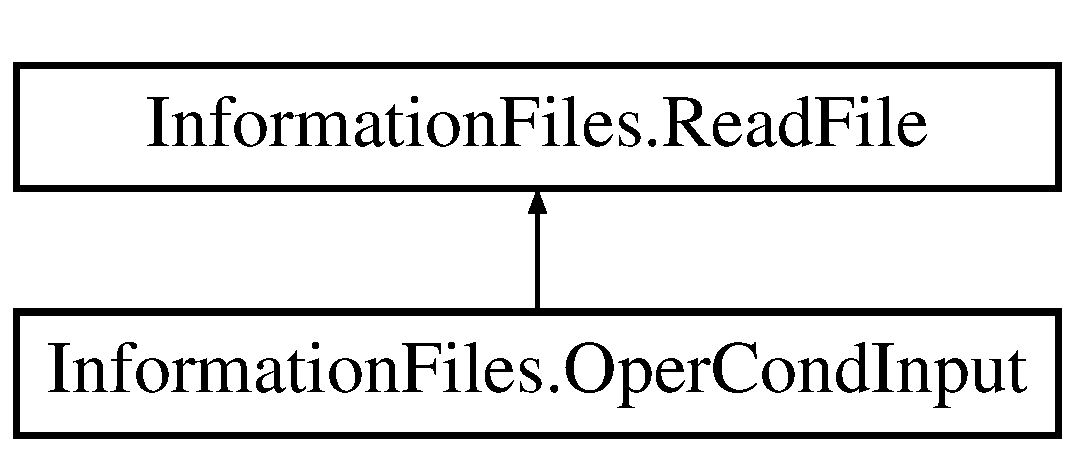
\includegraphics[height=2.000000cm]{classInformationFiles_1_1ReadFile}
\end{center}
\end{figure}
\subsection*{\-Public \-Member \-Functions}
\begin{DoxyCompactItemize}
\item 
\hypertarget{classInformationFiles_1_1ReadFile_ade33b94049e1245d790563a2988df6b0}{def {\bfseries \-\_\-\-\_\-init\-\_\-\-\_\-}}\label{classInformationFiles_1_1ReadFile_ade33b94049e1245d790563a2988df6b0}

\item 
def \hyperlink{classInformationFiles_1_1ReadFile_a33eb756d9e63ef0f7e0ad1c175406ef0}{read\-Lines}
\item 
def \hyperlink{classInformationFiles_1_1ReadFile_a259b8dd2f0754fe46c67e1af6c82ec5d}{\-Use\-Pyrol\-Progr}
\item 
def \hyperlink{classInformationFiles_1_1ReadFile_acbbf6f298c76c66d18d56c787225fcb7}{\-Fitting}
\item 
def \hyperlink{classInformationFiles_1_1ReadFile_a2911cbdb92a645b6114feca74fc69aba}{get\-Value}
\item 
def \hyperlink{classInformationFiles_1_1ReadFile_ae3432e04c7dde26bbcdb97d4436c1d70}{get\-Text}
\end{DoxyCompactItemize}
\subsection*{\-Public \-Attributes}
\begin{DoxyCompactItemize}
\item 
\hypertarget{classInformationFiles_1_1ReadFile_a129e3d7eee05b28541056afe51d3592a}{{\bfseries \-Input\-File}}\label{classInformationFiles_1_1ReadFile_a129e3d7eee05b28541056afe51d3592a}

\item 
\hypertarget{classInformationFiles_1_1ReadFile_a0c7c8f211c8642e3f3d66d5c3f9e585a}{{\bfseries \-Input}}\label{classInformationFiles_1_1ReadFile_a0c7c8f211c8642e3f3d66d5c3f9e585a}

\end{DoxyCompactItemize}


\subsection{\-Detailed \-Description}
\begin{DoxyVerb}general parent class for the reading objects CPDFile and FGDVCFile\end{DoxyVerb}
 

\subsection{\-Member \-Function \-Documentation}
\hypertarget{classInformationFiles_1_1ReadFile_acbbf6f298c76c66d18d56c787225fcb7}{\index{\-Information\-Files\-::\-Read\-File@{\-Information\-Files\-::\-Read\-File}!\-Fitting@{\-Fitting}}
\index{\-Fitting@{\-Fitting}!InformationFiles::ReadFile@{\-Information\-Files\-::\-Read\-File}}
\subsubsection[{\-Fitting}]{\setlength{\rightskip}{0pt plus 5cm}def {\bf \-Information\-Files.\-Read\-File.\-Fitting} (
\begin{DoxyParamCaption}
\item[{}]{self, }
\item[{}]{\-File\-Note}
\end{DoxyParamCaption}
)}}\label{classInformationFiles_1_1ReadFile_acbbf6f298c76c66d18d56c787225fcb7}
\begin{DoxyVerb}outputs the Fitting mode for Pyrolysis Program output (string: 'constantRate','Arrhenius','Kobayashi'). Possible input: 'constantRate', 'Arrhenius' or 'Kobayashi'\end{DoxyVerb}
 \hypertarget{classInformationFiles_1_1ReadFile_ae3432e04c7dde26bbcdb97d4436c1d70}{\index{\-Information\-Files\-::\-Read\-File@{\-Information\-Files\-::\-Read\-File}!get\-Text@{get\-Text}}
\index{get\-Text@{get\-Text}!InformationFiles::ReadFile@{\-Information\-Files\-::\-Read\-File}}
\subsubsection[{get\-Text}]{\setlength{\rightskip}{0pt plus 5cm}def {\bf \-Information\-Files.\-Read\-File.\-get\-Text} (
\begin{DoxyParamCaption}
\item[{}]{self, }
\item[{}]{\-File\-Note}
\end{DoxyParamCaption}
)}}\label{classInformationFiles_1_1ReadFile_ae3432e04c7dde26bbcdb97d4436c1d70}
\begin{DoxyVerb}output the data of the line below the FileNote as a string\end{DoxyVerb}
 \hypertarget{classInformationFiles_1_1ReadFile_a2911cbdb92a645b6114feca74fc69aba}{\index{\-Information\-Files\-::\-Read\-File@{\-Information\-Files\-::\-Read\-File}!get\-Value@{get\-Value}}
\index{get\-Value@{get\-Value}!InformationFiles::ReadFile@{\-Information\-Files\-::\-Read\-File}}
\subsubsection[{get\-Value}]{\setlength{\rightskip}{0pt plus 5cm}def {\bf \-Information\-Files.\-Read\-File.\-get\-Value} (
\begin{DoxyParamCaption}
\item[{}]{self, }
\item[{}]{\-File\-Note}
\end{DoxyParamCaption}
)}}\label{classInformationFiles_1_1ReadFile_a2911cbdb92a645b6114feca74fc69aba}
\begin{DoxyVerb}output the data of the line below the FileNote as a float\end{DoxyVerb}
 \hypertarget{classInformationFiles_1_1ReadFile_a33eb756d9e63ef0f7e0ad1c175406ef0}{\index{\-Information\-Files\-::\-Read\-File@{\-Information\-Files\-::\-Read\-File}!read\-Lines@{read\-Lines}}
\index{read\-Lines@{read\-Lines}!InformationFiles::ReadFile@{\-Information\-Files\-::\-Read\-File}}
\subsubsection[{read\-Lines}]{\setlength{\rightskip}{0pt plus 5cm}def {\bf \-Information\-Files.\-Read\-File.\-read\-Lines} (
\begin{DoxyParamCaption}
\item[{}]{self}
\end{DoxyParamCaption}
)}}\label{classInformationFiles_1_1ReadFile_a33eb756d9e63ef0f7e0ad1c175406ef0}
\begin{DoxyVerb}reads the input File line by line\end{DoxyVerb}
 \hypertarget{classInformationFiles_1_1ReadFile_a259b8dd2f0754fe46c67e1af6c82ec5d}{\index{\-Information\-Files\-::\-Read\-File@{\-Information\-Files\-::\-Read\-File}!\-Use\-Pyrol\-Progr@{\-Use\-Pyrol\-Progr}}
\index{\-Use\-Pyrol\-Progr@{\-Use\-Pyrol\-Progr}!InformationFiles::ReadFile@{\-Information\-Files\-::\-Read\-File}}
\subsubsection[{\-Use\-Pyrol\-Progr}]{\setlength{\rightskip}{0pt plus 5cm}def {\bf \-Information\-Files.\-Read\-File.\-Use\-Pyrol\-Progr} (
\begin{DoxyParamCaption}
\item[{}]{self, }
\item[{}]{\-File\-Note}
\end{DoxyParamCaption}
)}}\label{classInformationFiles_1_1ReadFile_a259b8dd2f0754fe46c67e1af6c82ec5d}
\begin{DoxyVerb}gets the information, whether Pyrolsis Program will be in use. Enter 'Yes' or 'True' for the case it should be used\end{DoxyVerb}
 

\-The documentation for this class was generated from the following file\-:\begin{DoxyCompactItemize}
\item 
/home/map/git/pkp/src/\-Information\-Files.\-py\end{DoxyCompactItemize}

\hypertarget{classCPD__SetAndLaunch_1_1SetterAndLauncher}{\section{\-C\-P\-D\-\_\-\-Set\-And\-Launch.\-Setter\-And\-Launcher \-Class \-Reference}
\label{classCPD__SetAndLaunch_1_1SetterAndLauncher}\index{\-C\-P\-D\-\_\-\-Set\-And\-Launch.\-Setter\-And\-Launcher@{\-C\-P\-D\-\_\-\-Set\-And\-Launch.\-Setter\-And\-Launcher}}
}
\subsection*{\-Public \-Member \-Functions}
\begin{DoxyCompactItemize}
\item 
\hypertarget{classCPD__SetAndLaunch_1_1SetterAndLauncher_ac539dfac1aea5e88cb89734a053a60ee}{def {\bfseries \-\_\-\-\_\-init\-\_\-\-\_\-}}\label{classCPD__SetAndLaunch_1_1SetterAndLauncher_ac539dfac1aea5e88cb89734a053a60ee}

\item 
def \hyperlink{classCPD__SetAndLaunch_1_1SetterAndLauncher_a073f7b4cfc2934f466b9d28e8fde9631}{\-Set\-Coal\-Parameter}
\item 
def \hyperlink{classCPD__SetAndLaunch_1_1SetterAndLauncher_a52eafb95b653d98273018cd07040b91d}{\-Set\-Operate\-Cond}
\item 
def \hyperlink{classCPD__SetAndLaunch_1_1SetterAndLauncher_aa39a02e314ebe1159026f46129fd2cd3}{\-Set\-Numerical\-Param}
\item 
def \hyperlink{classCPD__SetAndLaunch_1_1SetterAndLauncher_a61f9e53fe585c4333f54d90ba695296a}{\-Calc\-Coal\-Param}
\item 
def \hyperlink{classCPD__SetAndLaunch_1_1SetterAndLauncher_a5a8778ca01279308c247acd8fe4ea792}{write\-Instruct\-File}
\item 
def \hyperlink{classCPD__SetAndLaunch_1_1SetterAndLauncher_a20441720dcc1e49eb140bffdf730e719}{\-Run}
\end{DoxyCompactItemize}
\subsection*{\-Public \-Attributes}
\begin{DoxyCompactItemize}
\item 
\hypertarget{classCPD__SetAndLaunch_1_1SetterAndLauncher_a3c268b471849f02ffc1e559eee5d8afe}{{\bfseries ab}}\label{classCPD__SetAndLaunch_1_1SetterAndLauncher_a3c268b471849f02ffc1e559eee5d8afe}

\item 
\hypertarget{classCPD__SetAndLaunch_1_1SetterAndLauncher_a622b865e215eebe47a6ebceb0c1ef130}{{\bfseries eb}}\label{classCPD__SetAndLaunch_1_1SetterAndLauncher_a622b865e215eebe47a6ebceb0c1ef130}

\item 
\hypertarget{classCPD__SetAndLaunch_1_1SetterAndLauncher_a781d37517378b5948624be97a6488908}{{\bfseries ebsig}}\label{classCPD__SetAndLaunch_1_1SetterAndLauncher_a781d37517378b5948624be97a6488908}

\item 
\hypertarget{classCPD__SetAndLaunch_1_1SetterAndLauncher_aa7b60660c77b6dadbfd12a6387bb4ff2}{{\bfseries ac}}\label{classCPD__SetAndLaunch_1_1SetterAndLauncher_aa7b60660c77b6dadbfd12a6387bb4ff2}

\item 
\hypertarget{classCPD__SetAndLaunch_1_1SetterAndLauncher_a6a80c54a9fea15dc50a98e95592d1542}{{\bfseries ec}}\label{classCPD__SetAndLaunch_1_1SetterAndLauncher_a6a80c54a9fea15dc50a98e95592d1542}

\item 
\hypertarget{classCPD__SetAndLaunch_1_1SetterAndLauncher_ace4616c2c06a24f7057d522bda3dea21}{{\bfseries ag}}\label{classCPD__SetAndLaunch_1_1SetterAndLauncher_ace4616c2c06a24f7057d522bda3dea21}

\item 
\hypertarget{classCPD__SetAndLaunch_1_1SetterAndLauncher_ac7380ac8912cc9cf664e988b9e2e44dd}{{\bfseries eg}}\label{classCPD__SetAndLaunch_1_1SetterAndLauncher_ac7380ac8912cc9cf664e988b9e2e44dd}

\item 
\hypertarget{classCPD__SetAndLaunch_1_1SetterAndLauncher_a51bc79e5667d2d5d43c168625c98bf9e}{{\bfseries egsig}}\label{classCPD__SetAndLaunch_1_1SetterAndLauncher_a51bc79e5667d2d5d43c168625c98bf9e}

\item 
\hypertarget{classCPD__SetAndLaunch_1_1SetterAndLauncher_a5a202205f63453a753c11085497d2a92}{{\bfseries \-Acr}}\label{classCPD__SetAndLaunch_1_1SetterAndLauncher_a5a202205f63453a753c11085497d2a92}

\item 
\hypertarget{classCPD__SetAndLaunch_1_1SetterAndLauncher_a9f7e93e9970bde6892f62cb7a39ba087}{{\bfseries \-Ecr}}\label{classCPD__SetAndLaunch_1_1SetterAndLauncher_a9f7e93e9970bde6892f62cb7a39ba087}

\item 
\hypertarget{classCPD__SetAndLaunch_1_1SetterAndLauncher_a28e290c6359f73e1e91ebbe3e4522ea6}{{\bfseries arad}}\label{classCPD__SetAndLaunch_1_1SetterAndLauncher_a28e290c6359f73e1e91ebbe3e4522ea6}

\item 
\hypertarget{classCPD__SetAndLaunch_1_1SetterAndLauncher_aa45aecf36f0e807009b3230659620886}{{\bfseries erad}}\label{classCPD__SetAndLaunch_1_1SetterAndLauncher_aa45aecf36f0e807009b3230659620886}

\item 
\hypertarget{classCPD__SetAndLaunch_1_1SetterAndLauncher_aecaecbd9ed0ed2b5de8a5c98854916c2}{{\bfseries fstable}}\label{classCPD__SetAndLaunch_1_1SetterAndLauncher_aecaecbd9ed0ed2b5de8a5c98854916c2}

\item 
\hypertarget{classCPD__SetAndLaunch_1_1SetterAndLauncher_a8d4de53ccb76ba6fb3b0a7d9efe85538}{{\bfseries an}}\label{classCPD__SetAndLaunch_1_1SetterAndLauncher_a8d4de53ccb76ba6fb3b0a7d9efe85538}

\item 
\hypertarget{classCPD__SetAndLaunch_1_1SetterAndLauncher_a225d5d89c4db77e76bb1519b7bf15f19}{{\bfseries en}}\label{classCPD__SetAndLaunch_1_1SetterAndLauncher_a225d5d89c4db77e76bb1519b7bf15f19}

\item 
\hypertarget{classCPD__SetAndLaunch_1_1SetterAndLauncher_ae5534426bb6dddfac832e46bdafbc18b}{{\bfseries ensig}}\label{classCPD__SetAndLaunch_1_1SetterAndLauncher_ae5534426bb6dddfac832e46bdafbc18b}

\item 
\hypertarget{classCPD__SetAndLaunch_1_1SetterAndLauncher_abe4517b73acb86c0577d10a02eddc910}{{\bfseries nmax}}\label{classCPD__SetAndLaunch_1_1SetterAndLauncher_abe4517b73acb86c0577d10a02eddc910}

\item 
\hypertarget{classCPD__SetAndLaunch_1_1SetterAndLauncher_acd22d5942e9d420389261f048da015f0}{{\bfseries fcar}}\label{classCPD__SetAndLaunch_1_1SetterAndLauncher_acd22d5942e9d420389261f048da015f0}

\item 
\hypertarget{classCPD__SetAndLaunch_1_1SetterAndLauncher_a578e5d5911a4f60a0ff60170adf03597}{{\bfseries fhyd}}\label{classCPD__SetAndLaunch_1_1SetterAndLauncher_a578e5d5911a4f60a0ff60170adf03597}

\item 
\hypertarget{classCPD__SetAndLaunch_1_1SetterAndLauncher_af2ebb6cacfda0edab5e9619d4932c0c3}{{\bfseries fnit}}\label{classCPD__SetAndLaunch_1_1SetterAndLauncher_af2ebb6cacfda0edab5e9619d4932c0c3}

\item 
\hypertarget{classCPD__SetAndLaunch_1_1SetterAndLauncher_a2b4dd46223c5aea5b753282e7804969c}{{\bfseries foxy}}\label{classCPD__SetAndLaunch_1_1SetterAndLauncher_a2b4dd46223c5aea5b753282e7804969c}

\item 
\hypertarget{classCPD__SetAndLaunch_1_1SetterAndLauncher_a109661f3e201df3a894d53a3c9e3d55e}{{\bfseries \-V\-Mdaf}}\label{classCPD__SetAndLaunch_1_1SetterAndLauncher_a109661f3e201df3a894d53a3c9e3d55e}

\item 
\hypertarget{classCPD__SetAndLaunch_1_1SetterAndLauncher_a36b26d8c7a165fc34aee75112d409e6f}{{\bfseries pressure}}\label{classCPD__SetAndLaunch_1_1SetterAndLauncher_a36b26d8c7a165fc34aee75112d409e6f}

\item 
\hypertarget{classCPD__SetAndLaunch_1_1SetterAndLauncher_a36c8c09b5e25f01ab1ca148683b5d247}{{\bfseries \-T\-P}}\label{classCPD__SetAndLaunch_1_1SetterAndLauncher_a36c8c09b5e25f01ab1ca148683b5d247}

\item 
\hypertarget{classCPD__SetAndLaunch_1_1SetterAndLauncher_ac6dbac31787871db2c6780f25220cfc5}{{\bfseries dt}}\label{classCPD__SetAndLaunch_1_1SetterAndLauncher_ac6dbac31787871db2c6780f25220cfc5}

\item 
\hypertarget{classCPD__SetAndLaunch_1_1SetterAndLauncher_af793054ffde4d73388e5c928d099b045}{{\bfseries timax}}\label{classCPD__SetAndLaunch_1_1SetterAndLauncher_af793054ffde4d73388e5c928d099b045}

\item 
\hypertarget{classCPD__SetAndLaunch_1_1SetterAndLauncher_a5bcfe1fa3cc8634909ee962714186736}{{\bfseries c0}}\label{classCPD__SetAndLaunch_1_1SetterAndLauncher_a5bcfe1fa3cc8634909ee962714186736}

\item 
\hypertarget{classCPD__SetAndLaunch_1_1SetterAndLauncher_ac71614117cd4e0933cb10f3a24cf52e1}{{\bfseries mdel}}\label{classCPD__SetAndLaunch_1_1SetterAndLauncher_ac71614117cd4e0933cb10f3a24cf52e1}

\item 
\hypertarget{classCPD__SetAndLaunch_1_1SetterAndLauncher_a95301b646a1e25c09dadeff1ef1b9797}{{\bfseries mw}}\label{classCPD__SetAndLaunch_1_1SetterAndLauncher_a95301b646a1e25c09dadeff1ef1b9797}

\item 
\hypertarget{classCPD__SetAndLaunch_1_1SetterAndLauncher_adfa8dd137a5acabafdd566232e11db36}{{\bfseries p0}}\label{classCPD__SetAndLaunch_1_1SetterAndLauncher_adfa8dd137a5acabafdd566232e11db36}

\item 
\hypertarget{classCPD__SetAndLaunch_1_1SetterAndLauncher_a3984ed90521f966c0e16362b67ef88ab}{{\bfseries sig}}\label{classCPD__SetAndLaunch_1_1SetterAndLauncher_a3984ed90521f966c0e16362b67ef88ab}

\end{DoxyCompactItemize}


\subsection{\-Detailed \-Description}
\begin{DoxyVerb}This class is able to write the CPD input file and launch the CPD program. Before writing the CPD input file (method 'writeInstructFile') set all parameter using the corresponding methods (SetCoalParameter, SetOperateCond, SetNumericalParam, CalcCoalParam). After writing the instruct file, the .Run method can be used.\end{DoxyVerb}
 

\subsection{\-Member \-Function \-Documentation}
\hypertarget{classCPD__SetAndLaunch_1_1SetterAndLauncher_a61f9e53fe585c4333f54d90ba695296a}{\index{\-C\-P\-D\-\_\-\-Set\-And\-Launch\-::\-Setter\-And\-Launcher@{\-C\-P\-D\-\_\-\-Set\-And\-Launch\-::\-Setter\-And\-Launcher}!\-Calc\-Coal\-Param@{\-Calc\-Coal\-Param}}
\index{\-Calc\-Coal\-Param@{\-Calc\-Coal\-Param}!CPD_SetAndLaunch::SetterAndLauncher@{\-C\-P\-D\-\_\-\-Set\-And\-Launch\-::\-Setter\-And\-Launcher}}
\subsubsection[{\-Calc\-Coal\-Param}]{\setlength{\rightskip}{0pt plus 5cm}def {\bf \-C\-P\-D\-\_\-\-Set\-And\-Launch.\-Setter\-And\-Launcher.\-Calc\-Coal\-Param} (
\begin{DoxyParamCaption}
\item[{}]{self}
\end{DoxyParamCaption}
)}}\label{classCPD__SetAndLaunch_1_1SetterAndLauncher_a61f9e53fe585c4333f54d90ba695296a}
\begin{DoxyVerb}Calculates the CPD coal parameter mdel, mw, p0, sig and sets the as an attribute of the class.\end{DoxyVerb}
 \hypertarget{classCPD__SetAndLaunch_1_1SetterAndLauncher_a20441720dcc1e49eb140bffdf730e719}{\index{\-C\-P\-D\-\_\-\-Set\-And\-Launch\-::\-Setter\-And\-Launcher@{\-C\-P\-D\-\_\-\-Set\-And\-Launch\-::\-Setter\-And\-Launcher}!\-Run@{\-Run}}
\index{\-Run@{\-Run}!CPD_SetAndLaunch::SetterAndLauncher@{\-C\-P\-D\-\_\-\-Set\-And\-Launch\-::\-Setter\-And\-Launcher}}
\subsubsection[{\-Run}]{\setlength{\rightskip}{0pt plus 5cm}def {\bf \-C\-P\-D\-\_\-\-Set\-And\-Launch.\-Setter\-And\-Launcher.\-Run} (
\begin{DoxyParamCaption}
\item[{}]{self, }
\item[{}]{\-C\-P\-D\-\_\-exe, }
\item[{}]{\-Input\-\_\-\-File, }
\item[{}]{\-Log\-File}
\end{DoxyParamCaption}
)}}\label{classCPD__SetAndLaunch_1_1SetterAndLauncher_a20441720dcc1e49eb140bffdf730e719}
\begin{DoxyVerb}Launches CPD_exe and inputs Input_File. If the CPD executable is in another directory than the Python script enter the whole path for CPD_exe.\end{DoxyVerb}
 \hypertarget{classCPD__SetAndLaunch_1_1SetterAndLauncher_a073f7b4cfc2934f466b9d28e8fde9631}{\index{\-C\-P\-D\-\_\-\-Set\-And\-Launch\-::\-Setter\-And\-Launcher@{\-C\-P\-D\-\_\-\-Set\-And\-Launch\-::\-Setter\-And\-Launcher}!\-Set\-Coal\-Parameter@{\-Set\-Coal\-Parameter}}
\index{\-Set\-Coal\-Parameter@{\-Set\-Coal\-Parameter}!CPD_SetAndLaunch::SetterAndLauncher@{\-C\-P\-D\-\_\-\-Set\-And\-Launch\-::\-Setter\-And\-Launcher}}
\subsubsection[{\-Set\-Coal\-Parameter}]{\setlength{\rightskip}{0pt plus 5cm}def {\bf \-C\-P\-D\-\_\-\-Set\-And\-Launch.\-Setter\-And\-Launcher.\-Set\-Coal\-Parameter} (
\begin{DoxyParamCaption}
\item[{}]{self, }
\item[{}]{fcar, }
\item[{}]{fhyd, }
\item[{}]{fnit, }
\item[{}]{foxy, }
\item[{}]{\-V\-Mdaf}
\end{DoxyParamCaption}
)}}\label{classCPD__SetAndLaunch_1_1SetterAndLauncher_a073f7b4cfc2934f466b9d28e8fde9631}
\begin{DoxyVerb}Set the mass fraction of carbon (UA), hydrogen  (UA), nitrogen (UA), oxygen (UA) and the daf fraction of volatile matter (PA).\end{DoxyVerb}
 \hypertarget{classCPD__SetAndLaunch_1_1SetterAndLauncher_aa39a02e314ebe1159026f46129fd2cd3}{\index{\-C\-P\-D\-\_\-\-Set\-And\-Launch\-::\-Setter\-And\-Launcher@{\-C\-P\-D\-\_\-\-Set\-And\-Launch\-::\-Setter\-And\-Launcher}!\-Set\-Numerical\-Param@{\-Set\-Numerical\-Param}}
\index{\-Set\-Numerical\-Param@{\-Set\-Numerical\-Param}!CPD_SetAndLaunch::SetterAndLauncher@{\-C\-P\-D\-\_\-\-Set\-And\-Launch\-::\-Setter\-And\-Launcher}}
\subsubsection[{\-Set\-Numerical\-Param}]{\setlength{\rightskip}{0pt plus 5cm}def {\bf \-C\-P\-D\-\_\-\-Set\-And\-Launch.\-Setter\-And\-Launcher.\-Set\-Numerical\-Param} (
\begin{DoxyParamCaption}
\item[{}]{self, }
\item[{}]{dt, }
\item[{}]{timax}
\end{DoxyParamCaption}
)}}\label{classCPD__SetAndLaunch_1_1SetterAndLauncher_aa39a02e314ebe1159026f46129fd2cd3}
\begin{DoxyVerb}Sets the numerical parameter and the maximum simulation time. dt is a vector with the following information: [dt_initial,print-increment,dt_max]\end{DoxyVerb}
 \hypertarget{classCPD__SetAndLaunch_1_1SetterAndLauncher_a52eafb95b653d98273018cd07040b91d}{\index{\-C\-P\-D\-\_\-\-Set\-And\-Launch\-::\-Setter\-And\-Launcher@{\-C\-P\-D\-\_\-\-Set\-And\-Launch\-::\-Setter\-And\-Launcher}!\-Set\-Operate\-Cond@{\-Set\-Operate\-Cond}}
\index{\-Set\-Operate\-Cond@{\-Set\-Operate\-Cond}!CPD_SetAndLaunch::SetterAndLauncher@{\-C\-P\-D\-\_\-\-Set\-And\-Launch\-::\-Setter\-And\-Launcher}}
\subsubsection[{\-Set\-Operate\-Cond}]{\setlength{\rightskip}{0pt plus 5cm}def {\bf \-C\-P\-D\-\_\-\-Set\-And\-Launch.\-Setter\-And\-Launcher.\-Set\-Operate\-Cond} (
\begin{DoxyParamCaption}
\item[{}]{self, }
\item[{}]{pressure, }
\item[{}]{\-Time\-Temp}
\end{DoxyParamCaption}
)}}\label{classCPD__SetAndLaunch_1_1SetterAndLauncher_a52eafb95b653d98273018cd07040b91d}
\begin{DoxyVerb}Stes the operating condtions pressure and the time-temperature array. TimeTemp is an 2D-Array. One line of this array is [time_i,temp_i].\end{DoxyVerb}
 \hypertarget{classCPD__SetAndLaunch_1_1SetterAndLauncher_a5a8778ca01279308c247acd8fe4ea792}{\index{\-C\-P\-D\-\_\-\-Set\-And\-Launch\-::\-Setter\-And\-Launcher@{\-C\-P\-D\-\_\-\-Set\-And\-Launch\-::\-Setter\-And\-Launcher}!write\-Instruct\-File@{write\-Instruct\-File}}
\index{write\-Instruct\-File@{write\-Instruct\-File}!CPD_SetAndLaunch::SetterAndLauncher@{\-C\-P\-D\-\_\-\-Set\-And\-Launch\-::\-Setter\-And\-Launcher}}
\subsubsection[{write\-Instruct\-File}]{\setlength{\rightskip}{0pt plus 5cm}def {\bf \-C\-P\-D\-\_\-\-Set\-And\-Launch.\-Setter\-And\-Launcher.\-write\-Instruct\-File} (
\begin{DoxyParamCaption}
\item[{}]{self, }
\item[{}]{\-Dirpath}
\end{DoxyParamCaption}
)}}\label{classCPD__SetAndLaunch_1_1SetterAndLauncher_a5a8778ca01279308c247acd8fe4ea792}
\begin{DoxyVerb}Writes the File 'CPD_input.dat' into the directory Dirpath.\end{DoxyVerb}
 

\-The documentation for this class was generated from the following file\-:\begin{DoxyCompactItemize}
\item 
/home/map/git/pkp/src/\-C\-P\-D\-\_\-\-Set\-And\-Launch.\-py\end{DoxyCompactItemize}

\hypertarget{classPCCL__SetAndLaunch_1_1SetterAndLauncher}{\section{\-P\-C\-C\-L\-\_\-\-Set\-And\-Launch.\-Setter\-And\-Launcher \-Class \-Reference}
\label{classPCCL__SetAndLaunch_1_1SetterAndLauncher}\index{\-P\-C\-C\-L\-\_\-\-Set\-And\-Launch.\-Setter\-And\-Launcher@{\-P\-C\-C\-L\-\_\-\-Set\-And\-Launch.\-Setter\-And\-Launcher}}
}
\subsection*{\-Public \-Member \-Functions}
\begin{DoxyCompactItemize}
\item 
\hypertarget{classPCCL__SetAndLaunch_1_1SetterAndLauncher_aa03f8556a5cb80e4f52d2b5b3c39d975}{def {\bfseries \-\_\-\-\_\-init\-\_\-\-\_\-}}\label{classPCCL__SetAndLaunch_1_1SetterAndLauncher_aa03f8556a5cb80e4f52d2b5b3c39d975}

\item 
def \hyperlink{classPCCL__SetAndLaunch_1_1SetterAndLauncher_af3f49d80779a5ea202639fb2a0509676}{\-Set\-U\-A\-Coal\-Parameter}
\item 
def \hyperlink{classPCCL__SetAndLaunch_1_1SetterAndLauncher_a30eef6ccc6e5eb62188133bb555b68cf}{\-Set\-P\-A\-Coal\-Parameter}
\item 
def \hyperlink{classPCCL__SetAndLaunch_1_1SetterAndLauncher_a9cf2f451cc34a05c0f0590acbd0fce41}{\-Set\-Coal\-Calibration\-Factor}
\item 
def \hyperlink{classPCCL__SetAndLaunch_1_1SetterAndLauncher_a49fe3ae74111408b23dc7ee500fed547}{\-T\-Hist}
\item 
def \hyperlink{classPCCL__SetAndLaunch_1_1SetterAndLauncher_ae1127cd29781ebb1274c75ef065c3f18}{\-Set\-Pressure}
\item 
def \hyperlink{classPCCL__SetAndLaunch_1_1SetterAndLauncher_ab92a8919c69b10cf765a3fe1190b8710}{\-Set\-Particle\-Size}
\item 
def \hyperlink{classPCCL__SetAndLaunch_1_1SetterAndLauncher_acaaf7e0e2ac83d40fcae238cd412d7f6}{write\-Coal\-Files}
\item 
def \hyperlink{classPCCL__SetAndLaunch_1_1SetterAndLauncher_ac57f3501142f6cdf64ad0a0c922d2bac}{write\-Instruct\-Files}
\item 
def \hyperlink{classPCCL__SetAndLaunch_1_1SetterAndLauncher_a036a139dc6a77642ba3af0351b3d1391}{write\-Instruct\-Files\-Finish}
\item 
def \hyperlink{classPCCL__SetAndLaunch_1_1SetterAndLauncher_a501a8ba136753e46889143d32227a170}{\-Run}
\end{DoxyCompactItemize}
\subsection*{\-Public \-Attributes}
\begin{DoxyCompactItemize}
\item 
\hypertarget{classPCCL__SetAndLaunch_1_1SetterAndLauncher_a9eb80b936666ee182b5be15b23ba5313}{\hyperlink{classPCCL__SetAndLaunch_1_1SetterAndLauncher_a9eb80b936666ee182b5be15b23ba5313}{\-Test\-Reactor}}\label{classPCCL__SetAndLaunch_1_1SetterAndLauncher_a9eb80b936666ee182b5be15b23ba5313}

\begin{DoxyCompactList}\small\item\em \-T\-H\-E \-O\-P\-E\-R\-A\-T\-I\-N\-G \-C\-O\-N\-D\-I\-T\-I\-O\-N\-S \#\#\#. \end{DoxyCompactList}\item 
\hypertarget{classPCCL__SetAndLaunch_1_1SetterAndLauncher_a502e0306e7d1365c262a8e22236b3205}{{\bfseries \-Test\-Seq}}\label{classPCCL__SetAndLaunch_1_1SetterAndLauncher_a502e0306e7d1365c262a8e22236b3205}

\item 
\hypertarget{classPCCL__SetAndLaunch_1_1SetterAndLauncher_aac220493c2b3af58e1e14f7757cbbf30}{{\bfseries \-Output\-Res}}\label{classPCCL__SetAndLaunch_1_1SetterAndLauncher_aac220493c2b3af58e1e14f7757cbbf30}

\item 
\hypertarget{classPCCL__SetAndLaunch_1_1SetterAndLauncher_a64581d59f7f0289e6decb06586c284bb}{{\bfseries \-Gas}}\label{classPCCL__SetAndLaunch_1_1SetterAndLauncher_a64581d59f7f0289e6decb06586c284bb}

\item 
\hypertarget{classPCCL__SetAndLaunch_1_1SetterAndLauncher_a21f2fb28044ca5d8ec0d0df80cb37ac5}{{\bfseries \-Tinit}}\label{classPCCL__SetAndLaunch_1_1SetterAndLauncher_a21f2fb28044ca5d8ec0d0df80cb37ac5}

\item 
\hypertarget{classPCCL__SetAndLaunch_1_1SetterAndLauncher_a4b7aa2bc4b1395893e3819df0247261c}{{\bfseries \-Tultim}}\label{classPCCL__SetAndLaunch_1_1SetterAndLauncher_a4b7aa2bc4b1395893e3819df0247261c}

\item 
\hypertarget{classPCCL__SetAndLaunch_1_1SetterAndLauncher_a68d2986757cccc92fd8941401e0ff599}{{\bfseries \-Hr}}\label{classPCCL__SetAndLaunch_1_1SetterAndLauncher_a68d2986757cccc92fd8941401e0ff599}

\item 
\hypertarget{classPCCL__SetAndLaunch_1_1SetterAndLauncher_a6a3361b6107c95af5534d518e02789d5}{{\bfseries \-O2}}\label{classPCCL__SetAndLaunch_1_1SetterAndLauncher_a6a3361b6107c95af5534d518e02789d5}

\item 
\hypertarget{classPCCL__SetAndLaunch_1_1SetterAndLauncher_aa1ee2a1463bfdbbe5f1ef6fc470f95cf}{{\bfseries pressure}}\label{classPCCL__SetAndLaunch_1_1SetterAndLauncher_aa1ee2a1463bfdbbe5f1ef6fc470f95cf}

\item 
\hypertarget{classPCCL__SetAndLaunch_1_1SetterAndLauncher_aaebd06e9d5ae561e87f2227f6e701c6b}{{\bfseries t\-Hold}}\label{classPCCL__SetAndLaunch_1_1SetterAndLauncher_aaebd06e9d5ae561e87f2227f6e701c6b}

\item 
\hypertarget{classPCCL__SetAndLaunch_1_1SetterAndLauncher_aef0f47bc5fb3d49fec8a4940b4d8b270}{{\bfseries particle\-Diam}}\label{classPCCL__SetAndLaunch_1_1SetterAndLauncher_aef0f47bc5fb3d49fec8a4940b4d8b270}

\item 
\hypertarget{classPCCL__SetAndLaunch_1_1SetterAndLauncher_a8efc8259416a79f53bd369c48e8410c0}{{\bfseries \-R\-S}}\label{classPCCL__SetAndLaunch_1_1SetterAndLauncher_a8efc8259416a79f53bd369c48e8410c0}

\item 
\hypertarget{classPCCL__SetAndLaunch_1_1SetterAndLauncher_ae66f9ace65e372733007d266cec3b257}{{\bfseries \-R\-M}}\label{classPCCL__SetAndLaunch_1_1SetterAndLauncher_ae66f9ace65e372733007d266cec3b257}

\item 
\hypertarget{classPCCL__SetAndLaunch_1_1SetterAndLauncher_a7d019372c9c766aa566a8208a5ca6667}{{\bfseries \-S\-A}}\label{classPCCL__SetAndLaunch_1_1SetterAndLauncher_a7d019372c9c766aa566a8208a5ca6667}

\item 
\hypertarget{classPCCL__SetAndLaunch_1_1SetterAndLauncher_a885cd3a7c3ee5ef006480789b396a9e3}{\hyperlink{classPCCL__SetAndLaunch_1_1SetterAndLauncher_a885cd3a7c3ee5ef006480789b396a9e3}{\-Fuel}}\label{classPCCL__SetAndLaunch_1_1SetterAndLauncher_a885cd3a7c3ee5ef006480789b396a9e3}

\begin{DoxyCompactList}\small\item\em \-T\-H\-E \-C\-O\-A\-L \-P\-R\-O\-P\-E\-R\-T\-I\-E\-S \#\#\#. \end{DoxyCompactList}\item 
\hypertarget{classPCCL__SetAndLaunch_1_1SetterAndLauncher_aab18ed22345f12c9ceb84bcc9451fbde}{{\bfseries \-Coal\-Lable}}\label{classPCCL__SetAndLaunch_1_1SetterAndLauncher_aab18ed22345f12c9ceb84bcc9451fbde}

\item 
\hypertarget{classPCCL__SetAndLaunch_1_1SetterAndLauncher_a5fdf8847c1618f480b08c86f5d2640fa}{{\bfseries \-V\-M}}\label{classPCCL__SetAndLaunch_1_1SetterAndLauncher_a5fdf8847c1618f480b08c86f5d2640fa}

\item 
\hypertarget{classPCCL__SetAndLaunch_1_1SetterAndLauncher_a52fb8fa6d5be62d3e9f8c65bd75826a4}{{\bfseries \-F\-C}}\label{classPCCL__SetAndLaunch_1_1SetterAndLauncher_a52fb8fa6d5be62d3e9f8c65bd75826a4}

\item 
\hypertarget{classPCCL__SetAndLaunch_1_1SetterAndLauncher_af766eacf047684798f854329ec5e696b}{{\bfseries \-Moist}}\label{classPCCL__SetAndLaunch_1_1SetterAndLauncher_af766eacf047684798f854329ec5e696b}

\item 
\hypertarget{classPCCL__SetAndLaunch_1_1SetterAndLauncher_ae0ce9ea7ffbb3b0394314535a6d89fb1}{{\bfseries \-Ash}}\label{classPCCL__SetAndLaunch_1_1SetterAndLauncher_ae0ce9ea7ffbb3b0394314535a6d89fb1}

\item 
\hypertarget{classPCCL__SetAndLaunch_1_1SetterAndLauncher_a6202593ac99579a185f944210d1b7b45}{{\bfseries \-U\-A\-C}}\label{classPCCL__SetAndLaunch_1_1SetterAndLauncher_a6202593ac99579a185f944210d1b7b45}

\item 
\hypertarget{classPCCL__SetAndLaunch_1_1SetterAndLauncher_a9d7b8cf3c6c7d00d4c97238bdf5153f9}{{\bfseries \-U\-A\-H}}\label{classPCCL__SetAndLaunch_1_1SetterAndLauncher_a9d7b8cf3c6c7d00d4c97238bdf5153f9}

\item 
\hypertarget{classPCCL__SetAndLaunch_1_1SetterAndLauncher_a42ccff32a7b8369ae36e416edbb15f76}{{\bfseries \-U\-A\-O}}\label{classPCCL__SetAndLaunch_1_1SetterAndLauncher_a42ccff32a7b8369ae36e416edbb15f76}

\item 
\hypertarget{classPCCL__SetAndLaunch_1_1SetterAndLauncher_a4f07169b4c7c6b7474954f2a1034c683}{{\bfseries \-U\-A\-N}}\label{classPCCL__SetAndLaunch_1_1SetterAndLauncher_a4f07169b4c7c6b7474954f2a1034c683}

\item 
\hypertarget{classPCCL__SetAndLaunch_1_1SetterAndLauncher_ade2fb888fec59372d32a2b4cfd9092e2}{{\bfseries \-U\-A\-S}}\label{classPCCL__SetAndLaunch_1_1SetterAndLauncher_ade2fb888fec59372d32a2b4cfd9092e2}

\item 
\hypertarget{classPCCL__SetAndLaunch_1_1SetterAndLauncher_a09133fd4a276259c6ced0783b04ec184}{{\bfseries \-Calibr\-Factor}}\label{classPCCL__SetAndLaunch_1_1SetterAndLauncher_a09133fd4a276259c6ced0783b04ec184}

\item 
\hypertarget{classPCCL__SetAndLaunch_1_1SetterAndLauncher_af28440dda80da3d778a6172c307353ed}{{\bfseries \-Coal\-Counter}}\label{classPCCL__SetAndLaunch_1_1SetterAndLauncher_af28440dda80da3d778a6172c307353ed}

\item 
\hypertarget{classPCCL__SetAndLaunch_1_1SetterAndLauncher_ad3538b5a2ea4b4d43215be0196dc4477}{{\bfseries \-O\-C\-Counter}}\label{classPCCL__SetAndLaunch_1_1SetterAndLauncher_ad3538b5a2ea4b4d43215be0196dc4477}

\item 
\hypertarget{classPCCL__SetAndLaunch_1_1SetterAndLauncher_a05c3584089018f4c7c422f83848048e4}{{\bfseries \-Dir\-Path}}\label{classPCCL__SetAndLaunch_1_1SetterAndLauncher_a05c3584089018f4c7c422f83848048e4}

\end{DoxyCompactItemize}


\subsection{\-Detailed \-Description}
\begin{DoxyVerb}This class is able to write the PC Coal Lab input file and launch CPD program. Before writing the CPD input file (method 'writeInstructFile') set all parameter using the corresponding methods. After writing the instruct file, the .Run method can be used.\end{DoxyVerb}
 

\subsection{\-Member \-Function \-Documentation}
\hypertarget{classPCCL__SetAndLaunch_1_1SetterAndLauncher_a501a8ba136753e46889143d32227a170}{\index{\-P\-C\-C\-L\-\_\-\-Set\-And\-Launch\-::\-Setter\-And\-Launcher@{\-P\-C\-C\-L\-\_\-\-Set\-And\-Launch\-::\-Setter\-And\-Launcher}!\-Run@{\-Run}}
\index{\-Run@{\-Run}!PCCL_SetAndLaunch::SetterAndLauncher@{\-P\-C\-C\-L\-\_\-\-Set\-And\-Launch\-::\-Setter\-And\-Launcher}}
\subsubsection[{\-Run}]{\setlength{\rightskip}{0pt plus 5cm}def {\bf \-P\-C\-C\-L\-\_\-\-Set\-And\-Launch.\-Setter\-And\-Launcher.\-Run} (
\begin{DoxyParamCaption}
\item[{}]{self, }
\item[{}]{\-Path\-To\-Exe, }
\item[{}]{\-Name\-Of\-Exe}
\end{DoxyParamCaption}
)}}\label{classPCCL__SetAndLaunch_1_1SetterAndLauncher_a501a8ba136753e46889143d32227a170}
\begin{DoxyVerb}Launches PCCoV41M1to7Par.exe.\end{DoxyVerb}
 \hypertarget{classPCCL__SetAndLaunch_1_1SetterAndLauncher_a9cf2f451cc34a05c0f0590acbd0fce41}{\index{\-P\-C\-C\-L\-\_\-\-Set\-And\-Launch\-::\-Setter\-And\-Launcher@{\-P\-C\-C\-L\-\_\-\-Set\-And\-Launch\-::\-Setter\-And\-Launcher}!\-Set\-Coal\-Calibration\-Factor@{\-Set\-Coal\-Calibration\-Factor}}
\index{\-Set\-Coal\-Calibration\-Factor@{\-Set\-Coal\-Calibration\-Factor}!PCCL_SetAndLaunch::SetterAndLauncher@{\-P\-C\-C\-L\-\_\-\-Set\-And\-Launch\-::\-Setter\-And\-Launcher}}
\subsubsection[{\-Set\-Coal\-Calibration\-Factor}]{\setlength{\rightskip}{0pt plus 5cm}def {\bf \-P\-C\-C\-L\-\_\-\-Set\-And\-Launch.\-Setter\-And\-Launcher.\-Set\-Coal\-Calibration\-Factor} (
\begin{DoxyParamCaption}
\item[{}]{self, }
\item[{}]{\-Calibration\-Factor = {\ttfamily \-False}}
\end{DoxyParamCaption}
)}}\label{classPCCL__SetAndLaunch_1_1SetterAndLauncher_a9cf2f451cc34a05c0f0590acbd0fce41}
\begin{DoxyVerb}Here the PC Coal Lab Coal Calibration factor can be defined (float) if available.\end{DoxyVerb}
 \hypertarget{classPCCL__SetAndLaunch_1_1SetterAndLauncher_a30eef6ccc6e5eb62188133bb555b68cf}{\index{\-P\-C\-C\-L\-\_\-\-Set\-And\-Launch\-::\-Setter\-And\-Launcher@{\-P\-C\-C\-L\-\_\-\-Set\-And\-Launch\-::\-Setter\-And\-Launcher}!\-Set\-P\-A\-Coal\-Parameter@{\-Set\-P\-A\-Coal\-Parameter}}
\index{\-Set\-P\-A\-Coal\-Parameter@{\-Set\-P\-A\-Coal\-Parameter}!PCCL_SetAndLaunch::SetterAndLauncher@{\-P\-C\-C\-L\-\_\-\-Set\-And\-Launch\-::\-Setter\-And\-Launcher}}
\subsubsection[{\-Set\-P\-A\-Coal\-Parameter}]{\setlength{\rightskip}{0pt plus 5cm}def {\bf \-P\-C\-C\-L\-\_\-\-Set\-And\-Launch.\-Setter\-And\-Launcher.\-Set\-P\-A\-Coal\-Parameter} (
\begin{DoxyParamCaption}
\item[{}]{self, }
\item[{}]{volatile\-Matter, }
\item[{}]{fixed\-Carbon, }
\item[{}]{\-Moisture, }
\item[{}]{\-Ash}
\end{DoxyParamCaption}
)}}\label{classPCCL__SetAndLaunch_1_1SetterAndLauncher_a30eef6ccc6e5eb62188133bb555b68cf}
\begin{DoxyVerb}Sets the Proximate Analysis of the Coal using the as recieved state.\end{DoxyVerb}
 \hypertarget{classPCCL__SetAndLaunch_1_1SetterAndLauncher_ab92a8919c69b10cf765a3fe1190b8710}{\index{\-P\-C\-C\-L\-\_\-\-Set\-And\-Launch\-::\-Setter\-And\-Launcher@{\-P\-C\-C\-L\-\_\-\-Set\-And\-Launch\-::\-Setter\-And\-Launcher}!\-Set\-Particle\-Size@{\-Set\-Particle\-Size}}
\index{\-Set\-Particle\-Size@{\-Set\-Particle\-Size}!PCCL_SetAndLaunch::SetterAndLauncher@{\-P\-C\-C\-L\-\_\-\-Set\-And\-Launch\-::\-Setter\-And\-Launcher}}
\subsubsection[{\-Set\-Particle\-Size}]{\setlength{\rightskip}{0pt plus 5cm}def {\bf \-P\-C\-C\-L\-\_\-\-Set\-And\-Launch.\-Setter\-And\-Launcher.\-Set\-Particle\-Size} (
\begin{DoxyParamCaption}
\item[{}]{self, }
\item[{}]{\-Diameterin\-Microns}
\end{DoxyParamCaption}
)}}\label{classPCCL__SetAndLaunch_1_1SetterAndLauncher_ab92a8919c69b10cf765a3fe1190b8710}
\begin{DoxyVerb}Defines the particle diameter. Input it in micrometer.\end{DoxyVerb}
 \hypertarget{classPCCL__SetAndLaunch_1_1SetterAndLauncher_ae1127cd29781ebb1274c75ef065c3f18}{\index{\-P\-C\-C\-L\-\_\-\-Set\-And\-Launch\-::\-Setter\-And\-Launcher@{\-P\-C\-C\-L\-\_\-\-Set\-And\-Launch\-::\-Setter\-And\-Launcher}!\-Set\-Pressure@{\-Set\-Pressure}}
\index{\-Set\-Pressure@{\-Set\-Pressure}!PCCL_SetAndLaunch::SetterAndLauncher@{\-P\-C\-C\-L\-\_\-\-Set\-And\-Launch\-::\-Setter\-And\-Launcher}}
\subsubsection[{\-Set\-Pressure}]{\setlength{\rightskip}{0pt plus 5cm}def {\bf \-P\-C\-C\-L\-\_\-\-Set\-And\-Launch.\-Setter\-And\-Launcher.\-Set\-Pressure} (
\begin{DoxyParamCaption}
\item[{}]{self, }
\item[{}]{pressure}
\end{DoxyParamCaption}
)}}\label{classPCCL__SetAndLaunch_1_1SetterAndLauncher_ae1127cd29781ebb1274c75ef065c3f18}
\begin{DoxyVerb}Defines the pressure in atm\end{DoxyVerb}
 \hypertarget{classPCCL__SetAndLaunch_1_1SetterAndLauncher_af3f49d80779a5ea202639fb2a0509676}{\index{\-P\-C\-C\-L\-\_\-\-Set\-And\-Launch\-::\-Setter\-And\-Launcher@{\-P\-C\-C\-L\-\_\-\-Set\-And\-Launch\-::\-Setter\-And\-Launcher}!\-Set\-U\-A\-Coal\-Parameter@{\-Set\-U\-A\-Coal\-Parameter}}
\index{\-Set\-U\-A\-Coal\-Parameter@{\-Set\-U\-A\-Coal\-Parameter}!PCCL_SetAndLaunch::SetterAndLauncher@{\-P\-C\-C\-L\-\_\-\-Set\-And\-Launch\-::\-Setter\-And\-Launcher}}
\subsubsection[{\-Set\-U\-A\-Coal\-Parameter}]{\setlength{\rightskip}{0pt plus 5cm}def {\bf \-P\-C\-C\-L\-\_\-\-Set\-And\-Launch.\-Setter\-And\-Launcher.\-Set\-U\-A\-Coal\-Parameter} (
\begin{DoxyParamCaption}
\item[{}]{self, }
\item[{}]{fcar, }
\item[{}]{fhyd, }
\item[{}]{fnit, }
\item[{}]{foxy, }
\item[{}]{fsul = {\ttfamily 0.0}}
\end{DoxyParamCaption}
)}}\label{classPCCL__SetAndLaunch_1_1SetterAndLauncher_af3f49d80779a5ea202639fb2a0509676}
\begin{DoxyVerb}Set the mass fraction of carbon, hydrogen, nitrogen, oxygen and sulfur (there is standard is zero).\end{DoxyVerb}
 \hypertarget{classPCCL__SetAndLaunch_1_1SetterAndLauncher_a49fe3ae74111408b23dc7ee500fed547}{\index{\-P\-C\-C\-L\-\_\-\-Set\-And\-Launch\-::\-Setter\-And\-Launcher@{\-P\-C\-C\-L\-\_\-\-Set\-And\-Launch\-::\-Setter\-And\-Launcher}!\-T\-Hist@{\-T\-Hist}}
\index{\-T\-Hist@{\-T\-Hist}!PCCL_SetAndLaunch::SetterAndLauncher@{\-P\-C\-C\-L\-\_\-\-Set\-And\-Launch\-::\-Setter\-And\-Launcher}}
\subsubsection[{\-T\-Hist}]{\setlength{\rightskip}{0pt plus 5cm}def {\bf \-P\-C\-C\-L\-\_\-\-Set\-And\-Launch.\-Setter\-And\-Launcher.\-T\-Hist} (
\begin{DoxyParamCaption}
\item[{}]{self, }
\item[{}]{\-Tstart, }
\item[{}]{t1, }
\item[{}]{\-Tfinal, }
\item[{}]{tfinal}
\end{DoxyParamCaption}
)}}\label{classPCCL__SetAndLaunch_1_1SetterAndLauncher_a49fe3ae74111408b23dc7ee500fed547}
\begin{DoxyVerb}Define the heating rate ramp. Therefore enter the Start Temperature, the Temperature and time when the linear heating ends and the final Temperature and time. All are in Kelvin and are converted into Degree Celsius.\end{DoxyVerb}
 \hypertarget{classPCCL__SetAndLaunch_1_1SetterAndLauncher_acaaf7e0e2ac83d40fcae238cd412d7f6}{\index{\-P\-C\-C\-L\-\_\-\-Set\-And\-Launch\-::\-Setter\-And\-Launcher@{\-P\-C\-C\-L\-\_\-\-Set\-And\-Launch\-::\-Setter\-And\-Launcher}!write\-Coal\-Files@{write\-Coal\-Files}}
\index{write\-Coal\-Files@{write\-Coal\-Files}!PCCL_SetAndLaunch::SetterAndLauncher@{\-P\-C\-C\-L\-\_\-\-Set\-And\-Launch\-::\-Setter\-And\-Launcher}}
\subsubsection[{write\-Coal\-Files}]{\setlength{\rightskip}{0pt plus 5cm}def {\bf \-P\-C\-C\-L\-\_\-\-Set\-And\-Launch.\-Setter\-And\-Launcher.\-write\-Coal\-Files} (
\begin{DoxyParamCaption}
\item[{}]{self, }
\item[{}]{\-Dirpath, }
\item[{}]{mk\-New\-File = {\ttfamily \-False}}
\end{DoxyParamCaption}
)}}\label{classPCCL__SetAndLaunch_1_1SetterAndLauncher_acaaf7e0e2ac83d40fcae238cd412d7f6}
\begin{DoxyVerb}Writes the Coal File 'Coalpc.dat' into the given path.\end{DoxyVerb}
 \hypertarget{classPCCL__SetAndLaunch_1_1SetterAndLauncher_ac57f3501142f6cdf64ad0a0c922d2bac}{\index{\-P\-C\-C\-L\-\_\-\-Set\-And\-Launch\-::\-Setter\-And\-Launcher@{\-P\-C\-C\-L\-\_\-\-Set\-And\-Launch\-::\-Setter\-And\-Launcher}!write\-Instruct\-Files@{write\-Instruct\-Files}}
\index{write\-Instruct\-Files@{write\-Instruct\-Files}!PCCL_SetAndLaunch::SetterAndLauncher@{\-P\-C\-C\-L\-\_\-\-Set\-And\-Launch\-::\-Setter\-And\-Launcher}}
\subsubsection[{write\-Instruct\-Files}]{\setlength{\rightskip}{0pt plus 5cm}def {\bf \-P\-C\-C\-L\-\_\-\-Set\-And\-Launch.\-Setter\-And\-Launcher.\-write\-Instruct\-Files} (
\begin{DoxyParamCaption}
\item[{}]{self, }
\item[{}]{\-Dirpath, }
\item[{}]{mk\-New\-File = {\ttfamily \-False}}
\end{DoxyParamCaption}
)}}\label{classPCCL__SetAndLaunch_1_1SetterAndLauncher_ac57f3501142f6cdf64ad0a0c922d2bac}
\begin{DoxyVerb}Writes the Testplan File 'Testplan.dat' into the given path. If New File is set to True, a new one is generated. Otherwise the next lines are added to the existing Testplan.dat\end{DoxyVerb}
 \hypertarget{classPCCL__SetAndLaunch_1_1SetterAndLauncher_a036a139dc6a77642ba3af0351b3d1391}{\index{\-P\-C\-C\-L\-\_\-\-Set\-And\-Launch\-::\-Setter\-And\-Launcher@{\-P\-C\-C\-L\-\_\-\-Set\-And\-Launch\-::\-Setter\-And\-Launcher}!write\-Instruct\-Files\-Finish@{write\-Instruct\-Files\-Finish}}
\index{write\-Instruct\-Files\-Finish@{write\-Instruct\-Files\-Finish}!PCCL_SetAndLaunch::SetterAndLauncher@{\-P\-C\-C\-L\-\_\-\-Set\-And\-Launch\-::\-Setter\-And\-Launcher}}
\subsubsection[{write\-Instruct\-Files\-Finish}]{\setlength{\rightskip}{0pt plus 5cm}def {\bf \-P\-C\-C\-L\-\_\-\-Set\-And\-Launch.\-Setter\-And\-Launcher.\-write\-Instruct\-Files\-Finish} (
\begin{DoxyParamCaption}
\item[{}]{self}
\end{DoxyParamCaption}
)}}\label{classPCCL__SetAndLaunch_1_1SetterAndLauncher_a036a139dc6a77642ba3af0351b3d1391}
\begin{DoxyVerb}Writes the last statements into the Instruct File to finish it.\end{DoxyVerb}
 

\-The documentation for this class was generated from the following file\-:\begin{DoxyCompactItemize}
\item 
/home/map/git/pkp/src/\-P\-C\-C\-L\-\_\-\-Set\-And\-Launch.\-py\end{DoxyCompactItemize}

\hypertarget{classFGDVC__SetAndLaunch_1_1SetterAndLauncher}{\section{\-F\-G\-D\-V\-C\-\_\-\-Set\-And\-Launch.\-Setter\-And\-Launcher \-Class \-Reference}
\label{classFGDVC__SetAndLaunch_1_1SetterAndLauncher}\index{\-F\-G\-D\-V\-C\-\_\-\-Set\-And\-Launch.\-Setter\-And\-Launcher@{\-F\-G\-D\-V\-C\-\_\-\-Set\-And\-Launch.\-Setter\-And\-Launcher}}
}
\subsection*{\-Public \-Member \-Functions}
\begin{DoxyCompactItemize}
\item 
\hypertarget{classFGDVC__SetAndLaunch_1_1SetterAndLauncher_a8b91135b4f532768acc8fe5bd25ba657}{def {\bfseries \-\_\-\-\_\-init\-\_\-\-\_\-}}\label{classFGDVC__SetAndLaunch_1_1SetterAndLauncher_a8b91135b4f532768acc8fe5bd25ba657}

\item 
def \hyperlink{classFGDVC__SetAndLaunch_1_1SetterAndLauncher_a9be4d15cc143d24e54c19f19b3d67371}{set1\-Coal\-Location}
\item 
def \hyperlink{classFGDVC__SetAndLaunch_1_1SetterAndLauncher_af8d54375297836bc2af2b0584a9f8768}{set2\-Kin\-Location}
\item 
def \hyperlink{classFGDVC__SetAndLaunch_1_1SetterAndLauncher_aea7c95546b67bda52bf56f87b3644ef8}{set3\-Poly\-Location}
\item 
def \hyperlink{classFGDVC__SetAndLaunch_1_1SetterAndLauncher_aefc48598a3bc166370d2b403b443aec9}{set4\-Run\-I\-D}
\item 
def \hyperlink{classFGDVC__SetAndLaunch_1_1SetterAndLauncher_a0914fe6299f8ade1d7e17ee2483531cf}{set5\-Pressure}
\item 
def \hyperlink{classFGDVC__SetAndLaunch_1_1SetterAndLauncher_a116cb38b88fabe2f5bd2a45a1de6fa0b}{set6\-Theorie}
\item 
def \hyperlink{classFGDVC__SetAndLaunch_1_1SetterAndLauncher_a8572e0199ccb02da119c803c31331629}{set7\-Ramp}
\item 
def \hyperlink{classFGDVC__SetAndLaunch_1_1SetterAndLauncher_a85fddc035c436f83a141813db0fa0a4c}{set7\-File}
\item 
def \hyperlink{classFGDVC__SetAndLaunch_1_1SetterAndLauncher_aa7bc83c2215281993ec9cd513ddf3072}{set9\-Ash\-Moisture}
\item 
def \hyperlink{classFGDVC__SetAndLaunch_1_1SetterAndLauncher_a4066f0415203250464e57deb29d4cd0e}{set\-T\-Ramp\-\_\-or\-\_\-\-T\-File}
\item 
def \hyperlink{classFGDVC__SetAndLaunch_1_1SetterAndLauncher_a964768c47177ef9604fd7e4270fb1439}{write\-Instruct\-File}
\item 
def \hyperlink{classFGDVC__SetAndLaunch_1_1SetterAndLauncher_abca5677dd8d72bdf6116882a8f5a95d6}{\-Run}
\end{DoxyCompactItemize}
\subsection*{\-Public \-Attributes}
\begin{DoxyCompactItemize}
\item 
\hypertarget{classFGDVC__SetAndLaunch_1_1SetterAndLauncher_af7f22310acd15417a0e5f1bc297626b4}{{\bfseries \-Arguments1}}\label{classFGDVC__SetAndLaunch_1_1SetterAndLauncher_af7f22310acd15417a0e5f1bc297626b4}

\item 
\hypertarget{classFGDVC__SetAndLaunch_1_1SetterAndLauncher_a4accc4b2a50a765f5517ef73bf5061e7}{{\bfseries \-Arguments2}}\label{classFGDVC__SetAndLaunch_1_1SetterAndLauncher_a4accc4b2a50a765f5517ef73bf5061e7}

\item 
\hypertarget{classFGDVC__SetAndLaunch_1_1SetterAndLauncher_af941399e1fd5c4f091379215a21d854e}{{\bfseries \-Arguments3\-\_\-\-Ramp}}\label{classFGDVC__SetAndLaunch_1_1SetterAndLauncher_af941399e1fd5c4f091379215a21d854e}

\item 
\hypertarget{classFGDVC__SetAndLaunch_1_1SetterAndLauncher_aada7a41930084a8210fbaf5c713237b2}{{\bfseries \-Arguments3\-\_\-\-File}}\label{classFGDVC__SetAndLaunch_1_1SetterAndLauncher_aada7a41930084a8210fbaf5c713237b2}

\item 
\hypertarget{classFGDVC__SetAndLaunch_1_1SetterAndLauncher_ab0da1477203319c99229e06da1b06d00}{{\bfseries \-Arguments4}}\label{classFGDVC__SetAndLaunch_1_1SetterAndLauncher_ab0da1477203319c99229e06da1b06d00}

\item 
\hypertarget{classFGDVC__SetAndLaunch_1_1SetterAndLauncher_abd860c779b518516cb603694562ca856}{{\bfseries selected\-T\-History}}\label{classFGDVC__SetAndLaunch_1_1SetterAndLauncher_abd860c779b518516cb603694562ca856}

\end{DoxyCompactItemize}


\subsection{\-Detailed \-Description}
\begin{DoxyVerb}This class is able to write the 'instruct.ini' and launch the 'fgdvcd.exe'. Before writing the instruct.ini (method 'writeInstructFile') set all parameter using the corresponding methods (at least necessary: set1CoalLocation, set2KinLocation, set3PolyLocation, set5Pressure, set7Ramp). After writing the instruct file, the .Run method can be used.\end{DoxyVerb}
 

\subsection{\-Member \-Function \-Documentation}
\hypertarget{classFGDVC__SetAndLaunch_1_1SetterAndLauncher_abca5677dd8d72bdf6116882a8f5a95d6}{\index{\-F\-G\-D\-V\-C\-\_\-\-Set\-And\-Launch\-::\-Setter\-And\-Launcher@{\-F\-G\-D\-V\-C\-\_\-\-Set\-And\-Launch\-::\-Setter\-And\-Launcher}!\-Run@{\-Run}}
\index{\-Run@{\-Run}!FGDVC_SetAndLaunch::SetterAndLauncher@{\-F\-G\-D\-V\-C\-\_\-\-Set\-And\-Launch\-::\-Setter\-And\-Launcher}}
\subsubsection[{\-Run}]{\setlength{\rightskip}{0pt plus 5cm}def {\bf \-F\-G\-D\-V\-C\-\_\-\-Set\-And\-Launch.\-Setter\-And\-Launcher.\-Run} (
\begin{DoxyParamCaption}
\item[{}]{self, }
\item[{}]{\-Path\-From\-E\-X\-E}
\end{DoxyParamCaption}
)}}\label{classFGDVC__SetAndLaunch_1_1SetterAndLauncher_abca5677dd8d72bdf6116882a8f5a95d6}
\begin{DoxyVerb}Lauchnes fgdvcd.exe. The 'PathFromEXE' should not include the .exe and end with a backslash.\end{DoxyVerb}
 \hypertarget{classFGDVC__SetAndLaunch_1_1SetterAndLauncher_a9be4d15cc143d24e54c19f19b3d67371}{\index{\-F\-G\-D\-V\-C\-\_\-\-Set\-And\-Launch\-::\-Setter\-And\-Launcher@{\-F\-G\-D\-V\-C\-\_\-\-Set\-And\-Launch\-::\-Setter\-And\-Launcher}!set1\-Coal\-Location@{set1\-Coal\-Location}}
\index{set1\-Coal\-Location@{set1\-Coal\-Location}!FGDVC_SetAndLaunch::SetterAndLauncher@{\-F\-G\-D\-V\-C\-\_\-\-Set\-And\-Launch\-::\-Setter\-And\-Launcher}}
\subsubsection[{set1\-Coal\-Location}]{\setlength{\rightskip}{0pt plus 5cm}def {\bf \-F\-G\-D\-V\-C\-\_\-\-Set\-And\-Launch.\-Setter\-And\-Launcher.\-set1\-Coal\-Location} (
\begin{DoxyParamCaption}
\item[{}]{self, }
\item[{}]{\-Path\-Coal\-File}
\end{DoxyParamCaption}
)}}\label{classFGDVC__SetAndLaunch_1_1SetterAndLauncher_a9be4d15cc143d24e54c19f19b3d67371}
\begin{DoxyVerb}Sets the coal composition file directory.\end{DoxyVerb}
 \hypertarget{classFGDVC__SetAndLaunch_1_1SetterAndLauncher_af8d54375297836bc2af2b0584a9f8768}{\index{\-F\-G\-D\-V\-C\-\_\-\-Set\-And\-Launch\-::\-Setter\-And\-Launcher@{\-F\-G\-D\-V\-C\-\_\-\-Set\-And\-Launch\-::\-Setter\-And\-Launcher}!set2\-Kin\-Location@{set2\-Kin\-Location}}
\index{set2\-Kin\-Location@{set2\-Kin\-Location}!FGDVC_SetAndLaunch::SetterAndLauncher@{\-F\-G\-D\-V\-C\-\_\-\-Set\-And\-Launch\-::\-Setter\-And\-Launcher}}
\subsubsection[{set2\-Kin\-Location}]{\setlength{\rightskip}{0pt plus 5cm}def {\bf \-F\-G\-D\-V\-C\-\_\-\-Set\-And\-Launch.\-Setter\-And\-Launcher.\-set2\-Kin\-Location} (
\begin{DoxyParamCaption}
\item[{}]{self, }
\item[{}]{\-Path\-Kin\-File}
\end{DoxyParamCaption}
)}}\label{classFGDVC__SetAndLaunch_1_1SetterAndLauncher_af8d54375297836bc2af2b0584a9f8768}
\begin{DoxyVerb}Sets the coal kinetic file directory.\end{DoxyVerb}
 \hypertarget{classFGDVC__SetAndLaunch_1_1SetterAndLauncher_aea7c95546b67bda52bf56f87b3644ef8}{\index{\-F\-G\-D\-V\-C\-\_\-\-Set\-And\-Launch\-::\-Setter\-And\-Launcher@{\-F\-G\-D\-V\-C\-\_\-\-Set\-And\-Launch\-::\-Setter\-And\-Launcher}!set3\-Poly\-Location@{set3\-Poly\-Location}}
\index{set3\-Poly\-Location@{set3\-Poly\-Location}!FGDVC_SetAndLaunch::SetterAndLauncher@{\-F\-G\-D\-V\-C\-\_\-\-Set\-And\-Launch\-::\-Setter\-And\-Launcher}}
\subsubsection[{set3\-Poly\-Location}]{\setlength{\rightskip}{0pt plus 5cm}def {\bf \-F\-G\-D\-V\-C\-\_\-\-Set\-And\-Launch.\-Setter\-And\-Launcher.\-set3\-Poly\-Location} (
\begin{DoxyParamCaption}
\item[{}]{self, }
\item[{}]{\-Path\-Poly\-File}
\end{DoxyParamCaption}
)}}\label{classFGDVC__SetAndLaunch_1_1SetterAndLauncher_aea7c95546b67bda52bf56f87b3644ef8}
\begin{DoxyVerb}Sets the coal polymer file directory.\end{DoxyVerb}
 \hypertarget{classFGDVC__SetAndLaunch_1_1SetterAndLauncher_aefc48598a3bc166370d2b403b443aec9}{\index{\-F\-G\-D\-V\-C\-\_\-\-Set\-And\-Launch\-::\-Setter\-And\-Launcher@{\-F\-G\-D\-V\-C\-\_\-\-Set\-And\-Launch\-::\-Setter\-And\-Launcher}!set4\-Run\-I\-D@{set4\-Run\-I\-D}}
\index{set4\-Run\-I\-D@{set4\-Run\-I\-D}!FGDVC_SetAndLaunch::SetterAndLauncher@{\-F\-G\-D\-V\-C\-\_\-\-Set\-And\-Launch\-::\-Setter\-And\-Launcher}}
\subsubsection[{set4\-Run\-I\-D}]{\setlength{\rightskip}{0pt plus 5cm}def {\bf \-F\-G\-D\-V\-C\-\_\-\-Set\-And\-Launch.\-Setter\-And\-Launcher.\-set4\-Run\-I\-D} (
\begin{DoxyParamCaption}
\item[{}]{self, }
\item[{}]{pyrolysis\-O\-Rgeology}
\end{DoxyParamCaption}
)}}\label{classFGDVC__SetAndLaunch_1_1SetterAndLauncher_aefc48598a3bc166370d2b403b443aec9}
\begin{DoxyVerb}Sets weather the pyrolysis process or the geolegy process shall be modeled. For more information see FG-DVC manual.\end{DoxyVerb}
 \hypertarget{classFGDVC__SetAndLaunch_1_1SetterAndLauncher_a0914fe6299f8ade1d7e17ee2483531cf}{\index{\-F\-G\-D\-V\-C\-\_\-\-Set\-And\-Launch\-::\-Setter\-And\-Launcher@{\-F\-G\-D\-V\-C\-\_\-\-Set\-And\-Launch\-::\-Setter\-And\-Launcher}!set5\-Pressure@{set5\-Pressure}}
\index{set5\-Pressure@{set5\-Pressure}!FGDVC_SetAndLaunch::SetterAndLauncher@{\-F\-G\-D\-V\-C\-\_\-\-Set\-And\-Launch\-::\-Setter\-And\-Launcher}}
\subsubsection[{set5\-Pressure}]{\setlength{\rightskip}{0pt plus 5cm}def {\bf \-F\-G\-D\-V\-C\-\_\-\-Set\-And\-Launch.\-Setter\-And\-Launcher.\-set5\-Pressure} (
\begin{DoxyParamCaption}
\item[{}]{self, }
\item[{}]{\-Pressure\-In\-\_\-atm}
\end{DoxyParamCaption}
)}}\label{classFGDVC__SetAndLaunch_1_1SetterAndLauncher_a0914fe6299f8ade1d7e17ee2483531cf}
\begin{DoxyVerb}Sets the operating pressure (float).\end{DoxyVerb}
 \hypertarget{classFGDVC__SetAndLaunch_1_1SetterAndLauncher_a116cb38b88fabe2f5bd2a45a1de6fa0b}{\index{\-F\-G\-D\-V\-C\-\_\-\-Set\-And\-Launch\-::\-Setter\-And\-Launcher@{\-F\-G\-D\-V\-C\-\_\-\-Set\-And\-Launch\-::\-Setter\-And\-Launcher}!set6\-Theorie@{set6\-Theorie}}
\index{set6\-Theorie@{set6\-Theorie}!FGDVC_SetAndLaunch::SetterAndLauncher@{\-F\-G\-D\-V\-C\-\_\-\-Set\-And\-Launch\-::\-Setter\-And\-Launcher}}
\subsubsection[{set6\-Theorie}]{\setlength{\rightskip}{0pt plus 5cm}def {\bf \-F\-G\-D\-V\-C\-\_\-\-Set\-And\-Launch.\-Setter\-And\-Launcher.\-set6\-Theorie} (
\begin{DoxyParamCaption}
\item[{}]{self, }
\item[{}]{\-Theorie, }
\item[{}]{\-Residence\-Time}
\end{DoxyParamCaption}
)}}\label{classFGDVC__SetAndLaunch_1_1SetterAndLauncher_a116cb38b88fabe2f5bd2a45a1de6fa0b}
\begin{DoxyVerb}Sets the theory: 13 for no or partial tar cracking, 15 for full tar cracking. The residence input should be 0.0 for no tar cracking or a time greater zero for partial tar pressure. Full tar pressure also requires 0.0 as input, as it is the characteristic input of FG-DVC (although writing here 0.0, the full tar cracking is activated).\end{DoxyVerb}
 \hypertarget{classFGDVC__SetAndLaunch_1_1SetterAndLauncher_a85fddc035c436f83a141813db0fa0a4c}{\index{\-F\-G\-D\-V\-C\-\_\-\-Set\-And\-Launch\-::\-Setter\-And\-Launcher@{\-F\-G\-D\-V\-C\-\_\-\-Set\-And\-Launch\-::\-Setter\-And\-Launcher}!set7\-File@{set7\-File}}
\index{set7\-File@{set7\-File}!FGDVC_SetAndLaunch::SetterAndLauncher@{\-F\-G\-D\-V\-C\-\_\-\-Set\-And\-Launch\-::\-Setter\-And\-Launcher}}
\subsubsection[{set7\-File}]{\setlength{\rightskip}{0pt plus 5cm}def {\bf \-F\-G\-D\-V\-C\-\_\-\-Set\-And\-Launch.\-Setter\-And\-Launcher.\-set7\-File} (
\begin{DoxyParamCaption}
\item[{}]{self, }
\item[{}]{\-T\-History\-File\-Location}
\end{DoxyParamCaption}
)}}\label{classFGDVC__SetAndLaunch_1_1SetterAndLauncher_a85fddc035c436f83a141813db0fa0a4c}
\begin{DoxyVerb}For the case a temperature history shall be imported, this method should be used. 'THistoryFileLocation' is the directory of the .txt file containing two columns: first column the time in seconds, the second the temperature indegree Celsius-\end{DoxyVerb}
 \hypertarget{classFGDVC__SetAndLaunch_1_1SetterAndLauncher_a8572e0199ccb02da119c803c31331629}{\index{\-F\-G\-D\-V\-C\-\_\-\-Set\-And\-Launch\-::\-Setter\-And\-Launcher@{\-F\-G\-D\-V\-C\-\_\-\-Set\-And\-Launch\-::\-Setter\-And\-Launcher}!set7\-Ramp@{set7\-Ramp}}
\index{set7\-Ramp@{set7\-Ramp}!FGDVC_SetAndLaunch::SetterAndLauncher@{\-F\-G\-D\-V\-C\-\_\-\-Set\-And\-Launch\-::\-Setter\-And\-Launcher}}
\subsubsection[{set7\-Ramp}]{\setlength{\rightskip}{0pt plus 5cm}def {\bf \-F\-G\-D\-V\-C\-\_\-\-Set\-And\-Launch.\-Setter\-And\-Launcher.\-set7\-Ramp} (
\begin{DoxyParamCaption}
\item[{}]{self, }
\item[{}]{time\-Total, }
\item[{}]{dt, }
\item[{}]{d\-T, }
\item[{}]{final\-Pyrolysis\-Temp, }
\item[{}]{initial\-T, }
\item[{}]{\-Heating\-Rate}
\end{DoxyParamCaption}
)}}\label{classFGDVC__SetAndLaunch_1_1SetterAndLauncher_a8572e0199ccb02da119c803c31331629}
\begin{DoxyVerb}Sets the following time relevant and temperature history relevant parameter: the total simulation time 'timeTotal', the constant numerical time step 'dt', the maximum temperture step 'dT', the final pyrolysis temperature 'finalPyrolysisTemp', the temperature at t=0 'initialT', and the constant heating rate 'HeatingRate'. All these parameter are required for the case a linear heating rate should be modeled.\end{DoxyVerb}
 \hypertarget{classFGDVC__SetAndLaunch_1_1SetterAndLauncher_aa7bc83c2215281993ec9cd513ddf3072}{\index{\-F\-G\-D\-V\-C\-\_\-\-Set\-And\-Launch\-::\-Setter\-And\-Launcher@{\-F\-G\-D\-V\-C\-\_\-\-Set\-And\-Launch\-::\-Setter\-And\-Launcher}!set9\-Ash\-Moisture@{set9\-Ash\-Moisture}}
\index{set9\-Ash\-Moisture@{set9\-Ash\-Moisture}!FGDVC_SetAndLaunch::SetterAndLauncher@{\-F\-G\-D\-V\-C\-\_\-\-Set\-And\-Launch\-::\-Setter\-And\-Launcher}}
\subsubsection[{set9\-Ash\-Moisture}]{\setlength{\rightskip}{0pt plus 5cm}def {\bf \-F\-G\-D\-V\-C\-\_\-\-Set\-And\-Launch.\-Setter\-And\-Launcher.\-set9\-Ash\-Moisture} (
\begin{DoxyParamCaption}
\item[{}]{self, }
\item[{}]{\-Ash\-Content, }
\item[{}]{\-Moisture\-Content}
\end{DoxyParamCaption}
)}}\label{classFGDVC__SetAndLaunch_1_1SetterAndLauncher_aa7bc83c2215281993ec9cd513ddf3072}
\begin{DoxyVerb}Sets the amount of ash and moisture in the coal. By initializing the SetterAndLauncher object, both of these values are setted equal zero.\end{DoxyVerb}
 \hypertarget{classFGDVC__SetAndLaunch_1_1SetterAndLauncher_a4066f0415203250464e57deb29d4cd0e}{\index{\-F\-G\-D\-V\-C\-\_\-\-Set\-And\-Launch\-::\-Setter\-And\-Launcher@{\-F\-G\-D\-V\-C\-\_\-\-Set\-And\-Launch\-::\-Setter\-And\-Launcher}!set\-T\-Ramp\-\_\-or\-\_\-\-T\-File@{set\-T\-Ramp\-\_\-or\-\_\-\-T\-File}}
\index{set\-T\-Ramp\-\_\-or\-\_\-\-T\-File@{set\-T\-Ramp\-\_\-or\-\_\-\-T\-File}!FGDVC_SetAndLaunch::SetterAndLauncher@{\-F\-G\-D\-V\-C\-\_\-\-Set\-And\-Launch\-::\-Setter\-And\-Launcher}}
\subsubsection[{set\-T\-Ramp\-\_\-or\-\_\-\-T\-File}]{\setlength{\rightskip}{0pt plus 5cm}def {\bf \-F\-G\-D\-V\-C\-\_\-\-Set\-And\-Launch.\-Setter\-And\-Launcher.\-set\-T\-Ramp\-\_\-or\-\_\-\-T\-File} (
\begin{DoxyParamCaption}
\item[{}]{self, }
\item[{}]{select\-Ramp\-\_\-or\-\_\-\-File}
\end{DoxyParamCaption}
)}}\label{classFGDVC__SetAndLaunch_1_1SetterAndLauncher_a4066f0415203250464e57deb29d4cd0e}
\begin{DoxyVerb}Select weather the time should be defined using a linear ramp ('selectRamp_or_File'='Ramp') or with a input file ('selectRamp_or_File'='File').\end{DoxyVerb}
 \hypertarget{classFGDVC__SetAndLaunch_1_1SetterAndLauncher_a964768c47177ef9604fd7e4270fb1439}{\index{\-F\-G\-D\-V\-C\-\_\-\-Set\-And\-Launch\-::\-Setter\-And\-Launcher@{\-F\-G\-D\-V\-C\-\_\-\-Set\-And\-Launch\-::\-Setter\-And\-Launcher}!write\-Instruct\-File@{write\-Instruct\-File}}
\index{write\-Instruct\-File@{write\-Instruct\-File}!FGDVC_SetAndLaunch::SetterAndLauncher@{\-F\-G\-D\-V\-C\-\_\-\-Set\-And\-Launch\-::\-Setter\-And\-Launcher}}
\subsubsection[{write\-Instruct\-File}]{\setlength{\rightskip}{0pt plus 5cm}def {\bf \-F\-G\-D\-V\-C\-\_\-\-Set\-And\-Launch.\-Setter\-And\-Launcher.\-write\-Instruct\-File} (
\begin{DoxyParamCaption}
\item[{}]{self, }
\item[{}]{\-Filepath}
\end{DoxyParamCaption}
)}}\label{classFGDVC__SetAndLaunch_1_1SetterAndLauncher_a964768c47177ef9604fd7e4270fb1439}
\begin{DoxyVerb}Writes the File 'instruct.ini' into the directory 'Filepath', which should end with FGDVC_8-2-3/FGDVC .\end{DoxyVerb}
 

\-The documentation for this class was generated from the following file\-:\begin{DoxyCompactItemize}
\item 
/home/map/git/pkp/src/\-F\-G\-D\-V\-C\-\_\-\-Set\-And\-Launch.\-py\end{DoxyCompactItemize}

\hypertarget{classCompos__and__Energy_1_1SpeciesBalance}{\section{\-Compos\-\_\-and\-\_\-\-Energy.\-Species\-Balance \-Class \-Reference}
\label{classCompos__and__Energy_1_1SpeciesBalance}\index{\-Compos\-\_\-and\-\_\-\-Energy.\-Species\-Balance@{\-Compos\-\_\-and\-\_\-\-Energy.\-Species\-Balance}}
}
\-Inheritance diagram for \-Compos\-\_\-and\-\_\-\-Energy.\-Species\-Balance\-:\begin{figure}[H]
\begin{center}
\leavevmode
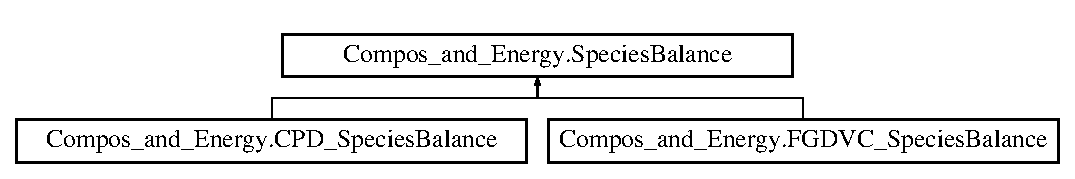
\includegraphics[height=1.951219cm]{classCompos__and__Energy_1_1SpeciesBalance}
\end{center}
\end{figure}
\subsection*{\-Public \-Member \-Functions}
\begin{DoxyCompactItemize}
\item 
def \hyperlink{classCompos__and__Energy_1_1SpeciesBalance_a5fec9a8d342543711abe2fc10632efb0}{\-Species\-Index}
\item 
def \hyperlink{classCompos__and__Energy_1_1SpeciesBalance_ae6b9b1a304a5b3686888725624c5e329}{moisture\-Volume\-Fraction}
\item 
def \hyperlink{classCompos__and__Energy_1_1SpeciesBalance_abeff1c726b62ba6c2d32173eb7f51d48}{\-Dulong}
\item 
def \hyperlink{classCompos__and__Energy_1_1SpeciesBalance_a05ae92b73a997e779c64bd2e6386a918}{correct\-U\-A}
\end{DoxyCompactItemize}
\subsection*{\-Static \-Public \-Attributes}
\begin{DoxyCompactItemize}
\item 
\hypertarget{classCompos__and__Energy_1_1SpeciesBalance_a57d64961c8e035bf8087528adf669379}{{\bfseries sum\-U\-A} = self.\-U\-A\-C+self.\-U\-A\-H+self.\-U\-A\-O+self.\-U\-A\-N+self.\-U\-A\-S}\label{classCompos__and__Energy_1_1SpeciesBalance_a57d64961c8e035bf8087528adf669379}

\end{DoxyCompactItemize}


\subsection{\-Detailed \-Description}
\begin{DoxyVerb}This is the parent Class for the CPD and FG-DVC specific Species Balances, containing general methods like the Dulong formular.\end{DoxyVerb}
 

\subsection{\-Member \-Function \-Documentation}
\hypertarget{classCompos__and__Energy_1_1SpeciesBalance_a05ae92b73a997e779c64bd2e6386a918}{\index{\-Compos\-\_\-and\-\_\-\-Energy\-::\-Species\-Balance@{\-Compos\-\_\-and\-\_\-\-Energy\-::\-Species\-Balance}!correct\-U\-A@{correct\-U\-A}}
\index{correct\-U\-A@{correct\-U\-A}!Compos_and_Energy::SpeciesBalance@{\-Compos\-\_\-and\-\_\-\-Energy\-::\-Species\-Balance}}
\subsubsection[{correct\-U\-A}]{\setlength{\rightskip}{0pt plus 5cm}def {\bf \-Compos\-\_\-and\-\_\-\-Energy.\-Species\-Balance.\-correct\-U\-A} (
\begin{DoxyParamCaption}
\item[{}]{self}
\end{DoxyParamCaption}
)}}\label{classCompos__and__Energy_1_1SpeciesBalance_a05ae92b73a997e779c64bd2e6386a918}
\begin{DoxyVerb}Scale Ultimate Analysis to have sum=1\end{DoxyVerb}
 \hypertarget{classCompos__and__Energy_1_1SpeciesBalance_abeff1c726b62ba6c2d32173eb7f51d48}{\index{\-Compos\-\_\-and\-\_\-\-Energy\-::\-Species\-Balance@{\-Compos\-\_\-and\-\_\-\-Energy\-::\-Species\-Balance}!\-Dulong@{\-Dulong}}
\index{\-Dulong@{\-Dulong}!Compos_and_Energy::SpeciesBalance@{\-Compos\-\_\-and\-\_\-\-Energy\-::\-Species\-Balance}}
\subsubsection[{\-Dulong}]{\setlength{\rightskip}{0pt plus 5cm}def {\bf \-Compos\-\_\-and\-\_\-\-Energy.\-Species\-Balance.\-Dulong} (
\begin{DoxyParamCaption}
\item[{}]{self}
\end{DoxyParamCaption}
)}}\label{classCompos__and__Energy_1_1SpeciesBalance_abeff1c726b62ba6c2d32173eb7f51d48}
\begin{DoxyVerb}Uses the Dulong formular to calculate the Higher heating value. The output is in J/kg.\end{DoxyVerb}
 \hypertarget{classCompos__and__Energy_1_1SpeciesBalance_ae6b9b1a304a5b3686888725624c5e329}{\index{\-Compos\-\_\-and\-\_\-\-Energy\-::\-Species\-Balance@{\-Compos\-\_\-and\-\_\-\-Energy\-::\-Species\-Balance}!moisture\-Volume\-Fraction@{moisture\-Volume\-Fraction}}
\index{moisture\-Volume\-Fraction@{moisture\-Volume\-Fraction}!Compos_and_Energy::SpeciesBalance@{\-Compos\-\_\-and\-\_\-\-Energy\-::\-Species\-Balance}}
\subsubsection[{moisture\-Volume\-Fraction}]{\setlength{\rightskip}{0pt plus 5cm}def {\bf \-Compos\-\_\-and\-\_\-\-Energy.\-Species\-Balance.\-moisture\-Volume\-Fraction} (
\begin{DoxyParamCaption}
\item[{}]{self}
\end{DoxyParamCaption}
)}}\label{classCompos__and__Energy_1_1SpeciesBalance_ae6b9b1a304a5b3686888725624c5e329}
\begin{DoxyVerb}
calculate volume fraction of moisture
\end{DoxyVerb}
 \hypertarget{classCompos__and__Energy_1_1SpeciesBalance_a5fec9a8d342543711abe2fc10632efb0}{\index{\-Compos\-\_\-and\-\_\-\-Energy\-::\-Species\-Balance@{\-Compos\-\_\-and\-\_\-\-Energy\-::\-Species\-Balance}!\-Species\-Index@{\-Species\-Index}}
\index{\-Species\-Index@{\-Species\-Index}!Compos_and_Energy::SpeciesBalance@{\-Compos\-\_\-and\-\_\-\-Energy\-::\-Species\-Balance}}
\subsubsection[{\-Species\-Index}]{\setlength{\rightskip}{0pt plus 5cm}def {\bf \-Compos\-\_\-and\-\_\-\-Energy.\-Species\-Balance.\-Species\-Index} (
\begin{DoxyParamCaption}
\item[{}]{self, }
\item[{}]{species}
\end{DoxyParamCaption}
)}}\label{classCompos__and__Energy_1_1SpeciesBalance_a5fec9a8d342543711abe2fc10632efb0}
\begin{DoxyVerb}Returns the column number of the input species.\end{DoxyVerb}
 

\-The documentation for this class was generated from the following file\-:\begin{DoxyCompactItemize}
\item 
/home/map/git/pkp/src/\-Compos\-\_\-and\-\_\-\-Energy.\-py\end{DoxyCompactItemize}

\hypertarget{classFitter_1_1TwoPointEstimator}{\section{\-Fitter.\-Two\-Point\-Estimator \-Class \-Reference}
\label{classFitter_1_1TwoPointEstimator}\index{\-Fitter.\-Two\-Point\-Estimator@{\-Fitter.\-Two\-Point\-Estimator}}
}
\subsection*{\-Public \-Member \-Functions}
\begin{DoxyCompactItemize}
\item 
\hypertarget{classFitter_1_1TwoPointEstimator_ac2100e8dc67ac0d999511f6e93d257c5}{def {\bfseries \-\_\-\-\_\-init\-\_\-\-\_\-}}\label{classFitter_1_1TwoPointEstimator_ac2100e8dc67ac0d999511f6e93d257c5}

\item 
\hypertarget{classFitter_1_1TwoPointEstimator_a1d30967d63d62fb4890f35a787ec1fca}{def {\bfseries estimate}}\label{classFitter_1_1TwoPointEstimator_a1d30967d63d62fb4890f35a787ec1fca}

\end{DoxyCompactItemize}
\subsection*{\-Static \-Public \-Attributes}
\begin{DoxyCompactItemize}
\item 
\hypertarget{classFitter_1_1TwoPointEstimator_acaedd1a44428e8d97bc109946e7334e4}{tuple {\bfseries t} = fgdvc.\-Time()}\label{classFitter_1_1TwoPointEstimator_acaedd1a44428e8d97bc109946e7334e4}

\item 
\hypertarget{classFitter_1_1TwoPointEstimator_a4394dafc36ec5b7a2555ded2a06b5a3b}{tuple {\bfseries \-Time\-Point} = int(\-Point\-Location$\ast$(fgdvc.\-N\-Points()))}\label{classFitter_1_1TwoPointEstimator_a4394dafc36ec5b7a2555ded2a06b5a3b}

\item 
\hypertarget{classFitter_1_1TwoPointEstimator_a7e2d9cfac4ed0e60e439bc682406a11d}{tuple {\bfseries \-V\-M\-\_\-s} = fgdvc.\-Mass\-V\-M\-\_\-s()}\label{classFitter_1_1TwoPointEstimator_a7e2d9cfac4ed0e60e439bc682406a11d}

\item 
\hypertarget{classFitter_1_1TwoPointEstimator_ac1eff0e06936424b0a7bbbd651a23b89}{list {\bfseries \-V\-M\-\_\-0} = \-V\-M\-\_\-s\mbox{[}0\mbox{]}}\label{classFitter_1_1TwoPointEstimator_ac1eff0e06936424b0a7bbbd651a23b89}

\item 
\hypertarget{classFitter_1_1TwoPointEstimator_abcfe43524bdecfa3fa0f9aea32ee72bc}{tuple {\bfseries k\-\_\-\-V\-M} = (np.\-log(\-V\-M\-\_\-s\mbox{[}\-Time\-Point\mbox{]}/\-V\-M\-\_\-0))}\label{classFitter_1_1TwoPointEstimator_abcfe43524bdecfa3fa0f9aea32ee72bc}

\item 
\hypertarget{classFitter_1_1TwoPointEstimator_ac9e2b04abd40aeca19dc2b3dfd9d7661}{tuple {\bfseries u} = fgdvc.\-Yield(\-Species)}\label{classFitter_1_1TwoPointEstimator_ac9e2b04abd40aeca19dc2b3dfd9d7661}

\item 
\hypertarget{classFitter_1_1TwoPointEstimator_a4680babf00753d73e67b22b0dc7dba34}{list {\bfseries u\-\_\-0} = u\mbox{[}-\/1\mbox{]}}\label{classFitter_1_1TwoPointEstimator_a4680babf00753d73e67b22b0dc7dba34}

\end{DoxyCompactItemize}


\subsection{\-Detailed \-Description}
\begin{DoxyVerb}Solves the devolatilization reaction analytically using two arbitrary selected points and the constant rate model. Unprecise. Should only be used for tests.\end{DoxyVerb}
 

\-The documentation for this class was generated from the following file\-:\begin{DoxyCompactItemize}
\item 
/home/map/git/pkp/src/\-Fitter.\-py\end{DoxyCompactItemize}

\hypertarget{classFit__one__run_1_1TwoPointEstimator}{\section{\-Fit\-\_\-one\-\_\-run.\-Two\-Point\-Estimator \-Class \-Reference}
\label{classFit__one__run_1_1TwoPointEstimator}\index{\-Fit\-\_\-one\-\_\-run.\-Two\-Point\-Estimator@{\-Fit\-\_\-one\-\_\-run.\-Two\-Point\-Estimator}}
}
\subsection*{\-Public \-Member \-Functions}
\begin{DoxyCompactItemize}
\item 
\hypertarget{classFit__one__run_1_1TwoPointEstimator_aff13b1525a0b59ba050a81c0c443c94d}{def {\bfseries \-\_\-\-\_\-init\-\_\-\-\_\-}}\label{classFit__one__run_1_1TwoPointEstimator_aff13b1525a0b59ba050a81c0c443c94d}

\item 
\hypertarget{classFit__one__run_1_1TwoPointEstimator_a5f9a818ca3b95720ca35bad0de1943bf}{def {\bfseries estimate}}\label{classFit__one__run_1_1TwoPointEstimator_a5f9a818ca3b95720ca35bad0de1943bf}

\end{DoxyCompactItemize}
\subsection*{\-Static \-Public \-Attributes}
\begin{DoxyCompactItemize}
\item 
\hypertarget{classFit__one__run_1_1TwoPointEstimator_a6c39dcbb0080c491a71ac30396aa0645}{tuple {\bfseries t} = fgdvc.\-Time()}\label{classFit__one__run_1_1TwoPointEstimator_a6c39dcbb0080c491a71ac30396aa0645}

\item 
\hypertarget{classFit__one__run_1_1TwoPointEstimator_ab3a7fb75aba8e43cffa61a1200b99544}{tuple {\bfseries \-Time\-Point} = int(\-Point\-Location$\ast$(fgdvc.\-N\-Points()))}\label{classFit__one__run_1_1TwoPointEstimator_ab3a7fb75aba8e43cffa61a1200b99544}

\item 
\hypertarget{classFit__one__run_1_1TwoPointEstimator_a5e0e5ecac04d21f9621680204b95703e}{tuple {\bfseries \-V\-M\-\_\-s} = fgdvc.\-Mass\-V\-M\-\_\-s()}\label{classFit__one__run_1_1TwoPointEstimator_a5e0e5ecac04d21f9621680204b95703e}

\item 
\hypertarget{classFit__one__run_1_1TwoPointEstimator_a1d81eb16e93c05a7b1b825dae06bcfd1}{list {\bfseries \-V\-M\-\_\-0} = \-V\-M\-\_\-s\mbox{[}0\mbox{]}}\label{classFit__one__run_1_1TwoPointEstimator_a1d81eb16e93c05a7b1b825dae06bcfd1}

\item 
\hypertarget{classFit__one__run_1_1TwoPointEstimator_a801660f443434df295bc9c05e88bcef8}{tuple {\bfseries k\-\_\-\-V\-M} = (np.\-log(\-V\-M\-\_\-s\mbox{[}\-Time\-Point\mbox{]}/\-V\-M\-\_\-0))}\label{classFit__one__run_1_1TwoPointEstimator_a801660f443434df295bc9c05e88bcef8}

\item 
\hypertarget{classFit__one__run_1_1TwoPointEstimator_abbd0ff8457dd988322c2cea1604a9a82}{tuple {\bfseries u} = fgdvc.\-Yield(\-Species)}\label{classFit__one__run_1_1TwoPointEstimator_abbd0ff8457dd988322c2cea1604a9a82}

\item 
\hypertarget{classFit__one__run_1_1TwoPointEstimator_a2e9224ae9f76276863605582c6950a3d}{list {\bfseries u\-\_\-0} = u\mbox{[}-\/1\mbox{]}}\label{classFit__one__run_1_1TwoPointEstimator_a2e9224ae9f76276863605582c6950a3d}

\end{DoxyCompactItemize}


\subsection{\-Detailed \-Description}
\begin{DoxyVerb}Solves the devolatilization reaction analytically using two arbitrary selected points and the constant rate model. Unprecise. Should only be used for tests.\end{DoxyVerb}
 

\-The documentation for this class was generated from the following file\-:\begin{DoxyCompactItemize}
\item 
/home/map/git/pkp/src/\-Fit\-\_\-one\-\_\-run.\-py\end{DoxyCompactItemize}

\hypertarget{classDone_1_1Ui__Dialog}{\section{\-Done.\-Ui\-\_\-\-Dialog \-Class \-Reference}
\label{classDone_1_1Ui__Dialog}\index{\-Done.\-Ui\-\_\-\-Dialog@{\-Done.\-Ui\-\_\-\-Dialog}}
}


\-The documentation for this class was generated from the following file\-:\begin{DoxyCompactItemize}
\item 
/home/map/git/pkp/\-Done.\-py\end{DoxyCompactItemize}

\hypertarget{classPKPgui_1_1Ui__PKP}{\section{\-P\-K\-Pgui.\-Ui\-\_\-\-P\-K\-P \-Class \-Reference}
\label{classPKPgui_1_1Ui__PKP}\index{\-P\-K\-Pgui.\-Ui\-\_\-\-P\-K\-P@{\-P\-K\-Pgui.\-Ui\-\_\-\-P\-K\-P}}
}
\subsection*{\-Public \-Member \-Functions}
\begin{DoxyCompactItemize}
\item 
\hypertarget{classPKPgui_1_1Ui__PKP_ae3e8bb330f8e3cb769a43b7248c9c210}{def {\bfseries setup\-Ui}}\label{classPKPgui_1_1Ui__PKP_ae3e8bb330f8e3cb769a43b7248c9c210}

\item 
def \hyperlink{classPKPgui_1_1Ui__PKP_a056261bf7b25d4ddbd57f34bae889c6b}{retranslate\-Ui}
\item 
def \hyperlink{classPKPgui_1_1Ui__PKP_a6ead41b34971c8aabce87fc75ff2a554}{\-Open\-Manual}
\item 
def \hyperlink{classPKPgui_1_1Ui__PKP_a27cc7ee90ecf2e67c8e4a2e68057be45}{\-Save\-Infos}
\item 
def \hyperlink{classPKPgui_1_1Ui__PKP_aea10bee40a0beade8419e79ddfa38b99}{\-Load\-Tt\-File1}
\item 
def \hyperlink{classPKPgui_1_1Ui__PKP_a1c3cc63f7da627d4cc8b5fc6a4d399aa}{\-Load\-Tt\-File2}
\item 
def \hyperlink{classPKPgui_1_1Ui__PKP_a6d84c002092b3c2a70985c37833757d2}{\-Load\-Tt\-File3}
\item 
def \hyperlink{classPKPgui_1_1Ui__PKP_a683a0a30a2c5c0675e04464b6475c4ad}{\-Load\-Tt\-File4}
\item 
def \hyperlink{classPKPgui_1_1Ui__PKP_a011acfe22957aab6d4381a5a2df1c16e}{\-Load\-Tt\-File5}
\item 
def \hyperlink{classPKPgui_1_1Ui__PKP_a1de23c077aacfb2e13cbc4fdc5be281f}{\-Plot1}
\item 
def \hyperlink{classPKPgui_1_1Ui__PKP_a7170dffb6875fb7d709ee7480b640885}{\-Plot2}
\item 
def \hyperlink{classPKPgui_1_1Ui__PKP_a01ec760c10b10938b73aa65267e86e1f}{\-Plot3}
\item 
def \hyperlink{classPKPgui_1_1Ui__PKP_aaf2cf4f8e6f8a0770e256a5810a6e132}{\-Plot4}
\item 
def \hyperlink{classPKPgui_1_1Ui__PKP_a158748bc711bd7c7182b4c482b1640e7}{\-Plot5}
\item 
def \hyperlink{classPKPgui_1_1Ui__PKP_a1678a6d812b5133f2a76f94203f90ef5}{\-Write\-Run}
\item 
def \hyperlink{classPKPgui_1_1Ui__PKP_a723ef4112a036ee96ad0fdcf35f3ee80}{\-Raise\-Error}
\item 
def \hyperlink{classPKPgui_1_1Ui__PKP_a9a4f443536282e39133ca3272ecce9d4}{\-Re\-Open\-Result\-Window}
\item 
\hypertarget{classPKPgui_1_1Ui__PKP_a56a74a85a72f50e6ea847313980da477}{def {\bfseries \-Load\-State}}\label{classPKPgui_1_1Ui__PKP_a56a74a85a72f50e6ea847313980da477}

\end{DoxyCompactItemize}
\subsection*{\-Public \-Attributes}
\begin{DoxyCompactItemize}
\item 
\hypertarget{classPKPgui_1_1Ui__PKP_ab7269f6483dbb170bd6a92f91540327c}{{\bfseries \-Q\-Widg\-Main}}\label{classPKPgui_1_1Ui__PKP_ab7269f6483dbb170bd6a92f91540327c}

\item 
\hypertarget{classPKPgui_1_1Ui__PKP_a40e9f4e9eec33a0cd9fe99638ff74dc0}{{\bfseries \-The\-Calculations\-Are\-Done}}\label{classPKPgui_1_1Ui__PKP_a40e9f4e9eec33a0cd9fe99638ff74dc0}

\item 
\hypertarget{classPKPgui_1_1Ui__PKP_af523c3ae6968ef5e99634258a6c5f597}{{\bfseries sv\-Info}}\label{classPKPgui_1_1Ui__PKP_af523c3ae6968ef5e99634258a6c5f597}

\item 
\hypertarget{classPKPgui_1_1Ui__PKP_a933fcfcad195c4a57f7792e00d8e956a}{{\bfseries centralwidget}}\label{classPKPgui_1_1Ui__PKP_a933fcfcad195c4a57f7792e00d8e956a}

\item 
\hypertarget{classPKPgui_1_1Ui__PKP_a502e2b01aa25572297cf395ea1df8688}{{\bfseries \-Header1\-\_\-2}}\label{classPKPgui_1_1Ui__PKP_a502e2b01aa25572297cf395ea1df8688}

\item 
\hypertarget{classPKPgui_1_1Ui__PKP_adf4619acfe12690d3a48b76a4cff5aef}{{\bfseries \-Header1}}\label{classPKPgui_1_1Ui__PKP_adf4619acfe12690d3a48b76a4cff5aef}

\item 
\hypertarget{classPKPgui_1_1Ui__PKP_a4fccecbcb51f16fe78b9801a7402717c}{{\bfseries \-Header2}}\label{classPKPgui_1_1Ui__PKP_a4fccecbcb51f16fe78b9801a7402717c}

\item 
\hypertarget{classPKPgui_1_1Ui__PKP_a79aeaa634451c6e5a4482a83744cdb30}{{\bfseries \-Header3}}\label{classPKPgui_1_1Ui__PKP_a79aeaa634451c6e5a4482a83744cdb30}

\item 
\hypertarget{classPKPgui_1_1Ui__PKP_ad7b1cc5f35b50bf41a35c34bb1789461}{{\bfseries l\-W\-\_\-\-Pyrol\-Pr\-Fit}}\label{classPKPgui_1_1Ui__PKP_ad7b1cc5f35b50bf41a35c34bb1789461}

\item 
\hypertarget{classPKPgui_1_1Ui__PKP_af8f85a996a304d1f36756f9ba03f2ad9}{{\bfseries l\-W\-\_\-\-Pyrol\-Pr\-Fit1}}\label{classPKPgui_1_1Ui__PKP_af8f85a996a304d1f36756f9ba03f2ad9}

\item 
\hypertarget{classPKPgui_1_1Ui__PKP_ad25eafd8fbcec3b95cebd1801de3a3e5}{{\bfseries l\-W\-\_\-\-Pyrol\-Pr\-Fit2}}\label{classPKPgui_1_1Ui__PKP_ad25eafd8fbcec3b95cebd1801de3a3e5}

\item 
\hypertarget{classPKPgui_1_1Ui__PKP_a7f9a9398beaa2475ca064725312f8848}{{\bfseries l\-W\-\_\-\-Pyrol\-Pr\-Fit3}}\label{classPKPgui_1_1Ui__PKP_a7f9a9398beaa2475ca064725312f8848}

\item 
\hypertarget{classPKPgui_1_1Ui__PKP_a17f62c4df7e4828daac1480e0fac0f35}{{\bfseries \-L\-\_\-\-F\-G\-D\-V\-C}}\label{classPKPgui_1_1Ui__PKP_a17f62c4df7e4828daac1480e0fac0f35}

\item 
\hypertarget{classPKPgui_1_1Ui__PKP_a92b702dccc32230561b79f9648e1e3f0}{{\bfseries \-L\-\_\-\-C\-P\-D}}\label{classPKPgui_1_1Ui__PKP_a92b702dccc32230561b79f9648e1e3f0}

\item 
\hypertarget{classPKPgui_1_1Ui__PKP_a9a3050d126fc46cf8c11847892a601fd}{{\bfseries \-L\-\_\-\-P\-C\-C\-L}}\label{classPKPgui_1_1Ui__PKP_a9a3050d126fc46cf8c11847892a601fd}

\item 
\hypertarget{classPKPgui_1_1Ui__PKP_ae34ff49c23c74bdc1f79097c8fd93435}{{\bfseries \-L\-\_\-\-Polimi}}\label{classPKPgui_1_1Ui__PKP_ae34ff49c23c74bdc1f79097c8fd93435}

\item 
\hypertarget{classPKPgui_1_1Ui__PKP_a49dde55a32802b1c003696ce1975569d}{{\bfseries \-L\-\_\-\-Weight\-Param}}\label{classPKPgui_1_1Ui__PKP_a49dde55a32802b1c003696ce1975569d}

\item 
\hypertarget{classPKPgui_1_1Ui__PKP_a23eee268ff9dd9b5f200963db53077c9}{{\bfseries \-L\-\_\-\-Yweight}}\label{classPKPgui_1_1Ui__PKP_a23eee268ff9dd9b5f200963db53077c9}

\item 
\hypertarget{classPKPgui_1_1Ui__PKP_a1a4de659de32da2042ab40985bd7f53d}{{\bfseries \-L\-\_\-\-Rweight}}\label{classPKPgui_1_1Ui__PKP_a1a4de659de32da2042ab40985bd7f53d}

\item 
\hypertarget{classPKPgui_1_1Ui__PKP_a66c8039d08d9094226b14d806ca51c4a}{{\bfseries \-L\-\_\-\-Arrh\-Spec1}}\label{classPKPgui_1_1Ui__PKP_a66c8039d08d9094226b14d806ca51c4a}

\item 
\hypertarget{classPKPgui_1_1Ui__PKP_af0916bc429c9f7b92cef6dd4a31db7d2}{{\bfseries \-L\-\_\-\-Arrh\-Spec2}}\label{classPKPgui_1_1Ui__PKP_af0916bc429c9f7b92cef6dd4a31db7d2}

\item 
\hypertarget{classPKPgui_1_1Ui__PKP_a0d69cefe65d2f90a88ba601b655865cf}{{\bfseries c\-B\-\_\-\-C\-P\-D}}\label{classPKPgui_1_1Ui__PKP_a0d69cefe65d2f90a88ba601b655865cf}

\item 
\hypertarget{classPKPgui_1_1Ui__PKP_a8b7197975385e3d54c0244fee260a51b}{{\bfseries c\-B\-\_\-\-F\-G\-D\-V\-C}}\label{classPKPgui_1_1Ui__PKP_a8b7197975385e3d54c0244fee260a51b}

\item 
\hypertarget{classPKPgui_1_1Ui__PKP_aabe03940099f7192466cb38fa3717cc7}{{\bfseries c\-B\-\_\-\-P\-C\-C\-L}}\label{classPKPgui_1_1Ui__PKP_aabe03940099f7192466cb38fa3717cc7}

\item 
\hypertarget{classPKPgui_1_1Ui__PKP_aa5cb71be2f50a366aa932ad94efc4656}{{\bfseries c\-B\-\_\-\-Polimi}}\label{classPKPgui_1_1Ui__PKP_aa5cb71be2f50a366aa932ad94efc4656}

\item 
\hypertarget{classPKPgui_1_1Ui__PKP_a0a0e9b68b3a8fb12f54b282a0cfa2418}{{\bfseries c\-B\-\_\-\-Arrh\-Spec}}\label{classPKPgui_1_1Ui__PKP_a0a0e9b68b3a8fb12f54b282a0cfa2418}

\item 
\hypertarget{classPKPgui_1_1Ui__PKP_a9ad4c6bb35b65e6ea831fe679e3326ae}{{\bfseries l\-E\-\_\-\-Yweight}}\label{classPKPgui_1_1Ui__PKP_a9ad4c6bb35b65e6ea831fe679e3326ae}

\item 
\hypertarget{classPKPgui_1_1Ui__PKP_a5854c8f33c9b9f3e3bf5c159c25be382}{{\bfseries l\-E\-\_\-\-Rweight}}\label{classPKPgui_1_1Ui__PKP_a5854c8f33c9b9f3e3bf5c159c25be382}

\item 
\hypertarget{classPKPgui_1_1Ui__PKP_a41f461a2e6c2f08f143ccf973c47d490}{{\bfseries g\-L\-\_\-\-Pyrol\-Pr\-Fit}}\label{classPKPgui_1_1Ui__PKP_a41f461a2e6c2f08f143ccf973c47d490}

\item 
\hypertarget{classPKPgui_1_1Ui__PKP_a4bf88dc11cb21d76914b24eb2a943e3d}{{\bfseries g\-L\-\_\-\-Pyrol\-Pr\-Fit1}}\label{classPKPgui_1_1Ui__PKP_a4bf88dc11cb21d76914b24eb2a943e3d}

\item 
\hypertarget{classPKPgui_1_1Ui__PKP_a0d1bf022d5dc06a5b9bff35f5d1b5483}{{\bfseries g\-L\-\_\-\-Pyrol\-Pr\-Fit2}}\label{classPKPgui_1_1Ui__PKP_a0d1bf022d5dc06a5b9bff35f5d1b5483}

\item 
\hypertarget{classPKPgui_1_1Ui__PKP_ad9ec8c1f677ec1d12717c1c7372b2d58}{{\bfseries g\-L\-\_\-\-Pyrol\-Pr\-Fit3}}\label{classPKPgui_1_1Ui__PKP_ad9ec8c1f677ec1d12717c1c7372b2d58}

\item 
\hypertarget{classPKPgui_1_1Ui__PKP_abd771e23d5637e5de7807aa590c6977b}{{\bfseries l\-W\-\_\-\-Coal}}\label{classPKPgui_1_1Ui__PKP_abd771e23d5637e5de7807aa590c6977b}

\item 
\hypertarget{classPKPgui_1_1Ui__PKP_ace3dac884a94064d3fab7fc662f6a813}{{\bfseries \-L\-\_\-\-U\-A}}\label{classPKPgui_1_1Ui__PKP_ace3dac884a94064d3fab7fc662f6a813}

\item 
\hypertarget{classPKPgui_1_1Ui__PKP_ac684655b18329877e9872dd4cab93745}{{\bfseries \-L\-\_\-\-U\-A\-C}}\label{classPKPgui_1_1Ui__PKP_ac684655b18329877e9872dd4cab93745}

\item 
\hypertarget{classPKPgui_1_1Ui__PKP_ae9fb7c76ab114452b0710b7dab792150}{{\bfseries l\-E\-\_\-\-U\-A\-C}}\label{classPKPgui_1_1Ui__PKP_ae9fb7c76ab114452b0710b7dab792150}

\item 
\hypertarget{classPKPgui_1_1Ui__PKP_a6bb8f5091b56b0a0d7b997f5ec0be1e0}{{\bfseries \-L\-\_\-\-U\-A\-H}}\label{classPKPgui_1_1Ui__PKP_a6bb8f5091b56b0a0d7b997f5ec0be1e0}

\item 
\hypertarget{classPKPgui_1_1Ui__PKP_a71b6135b3c8df66ae7ecc22c79f77815}{{\bfseries l\-E\-\_\-\-U\-A\-H}}\label{classPKPgui_1_1Ui__PKP_a71b6135b3c8df66ae7ecc22c79f77815}

\item 
\hypertarget{classPKPgui_1_1Ui__PKP_a6da9021b64bd76f5639dd52f4480f604}{{\bfseries \-L\-\_\-\-U\-A\-N}}\label{classPKPgui_1_1Ui__PKP_a6da9021b64bd76f5639dd52f4480f604}

\item 
\hypertarget{classPKPgui_1_1Ui__PKP_af2ed8c2085494ffb7ff7db7b2792f910}{{\bfseries l\-E\-\_\-\-U\-A\-N}}\label{classPKPgui_1_1Ui__PKP_af2ed8c2085494ffb7ff7db7b2792f910}

\item 
\hypertarget{classPKPgui_1_1Ui__PKP_a7c99a5131960b1b4d76ed6618280e83e}{{\bfseries \-L\-\_\-\-U\-A\-O}}\label{classPKPgui_1_1Ui__PKP_a7c99a5131960b1b4d76ed6618280e83e}

\item 
\hypertarget{classPKPgui_1_1Ui__PKP_ab4960413de56b4df413dcf1bbc3cd50a}{{\bfseries l\-E\-\_\-\-U\-A\-O}}\label{classPKPgui_1_1Ui__PKP_ab4960413de56b4df413dcf1bbc3cd50a}

\item 
\hypertarget{classPKPgui_1_1Ui__PKP_a129ae505b195aac6a954b48e94a1a3dc}{{\bfseries \-L\-\_\-\-U\-A\-S}}\label{classPKPgui_1_1Ui__PKP_a129ae505b195aac6a954b48e94a1a3dc}

\item 
\hypertarget{classPKPgui_1_1Ui__PKP_a69997e1f98a62617db8a64d915c54c87}{{\bfseries l\-E\-\_\-\-U\-A\-S}}\label{classPKPgui_1_1Ui__PKP_a69997e1f98a62617db8a64d915c54c87}

\item 
\hypertarget{classPKPgui_1_1Ui__PKP_afe7172d3b2d0be5af243e8e3c5429640}{{\bfseries \-L\-\_\-\-P\-A}}\label{classPKPgui_1_1Ui__PKP_afe7172d3b2d0be5af243e8e3c5429640}

\item 
\hypertarget{classPKPgui_1_1Ui__PKP_a277e6a9b2aef3597e74ef34ecdc3d2cd}{{\bfseries \-L\-\_\-\-P\-A\-F\-C}}\label{classPKPgui_1_1Ui__PKP_a277e6a9b2aef3597e74ef34ecdc3d2cd}

\item 
\hypertarget{classPKPgui_1_1Ui__PKP_a558d1b8a12d973f0bf8840bf9b86310b}{{\bfseries l\-E\-\_\-\-P\-A\-F\-C}}\label{classPKPgui_1_1Ui__PKP_a558d1b8a12d973f0bf8840bf9b86310b}

\item 
\hypertarget{classPKPgui_1_1Ui__PKP_ab27b1f1066233af2e5a993c695f54f08}{{\bfseries \-L\-\_\-\-P\-A\-V\-M}}\label{classPKPgui_1_1Ui__PKP_ab27b1f1066233af2e5a993c695f54f08}

\item 
\hypertarget{classPKPgui_1_1Ui__PKP_a06a3a75c550db66bde0dafcb794ccf0c}{{\bfseries l\-E\-\_\-\-P\-A\-V\-M}}\label{classPKPgui_1_1Ui__PKP_a06a3a75c550db66bde0dafcb794ccf0c}

\item 
\hypertarget{classPKPgui_1_1Ui__PKP_a17c856ac78ef03a85e51cc22ea4d5cea}{{\bfseries \-L\-\_\-\-P\-A\-Moi}}\label{classPKPgui_1_1Ui__PKP_a17c856ac78ef03a85e51cc22ea4d5cea}

\item 
\hypertarget{classPKPgui_1_1Ui__PKP_add6ee065d156b5fbba247ae9f20de3f3}{{\bfseries l\-E\-\_\-\-P\-A\-Moi}}\label{classPKPgui_1_1Ui__PKP_add6ee065d156b5fbba247ae9f20de3f3}

\item 
\hypertarget{classPKPgui_1_1Ui__PKP_a68ab9b4e2f7d3277c423488f9d03294b}{{\bfseries \-L\-\_\-\-P\-A\-Ash}}\label{classPKPgui_1_1Ui__PKP_a68ab9b4e2f7d3277c423488f9d03294b}

\item 
\hypertarget{classPKPgui_1_1Ui__PKP_a63cee9d3ae959e09b74ac79754eef080}{{\bfseries l\-E\-\_\-\-P\-A\-Ash}}\label{classPKPgui_1_1Ui__PKP_a63cee9d3ae959e09b74ac79754eef080}

\item 
\hypertarget{classPKPgui_1_1Ui__PKP_aac805cac03b6530291e08acc297c82bc}{{\bfseries \-L\-\_\-\-M\-W}}\label{classPKPgui_1_1Ui__PKP_aac805cac03b6530291e08acc297c82bc}

\item 
\hypertarget{classPKPgui_1_1Ui__PKP_ab41ef5354a004142625904cac1861eeb}{{\bfseries \-L\-\_\-\-M\-W\-Tar}}\label{classPKPgui_1_1Ui__PKP_ab41ef5354a004142625904cac1861eeb}

\item 
\hypertarget{classPKPgui_1_1Ui__PKP_a204665d55cb034a3e7d1a812ff69ecde}{{\bfseries l\-E\-\_\-\-M\-W\-Tar}}\label{classPKPgui_1_1Ui__PKP_a204665d55cb034a3e7d1a812ff69ecde}

\item 
\hypertarget{classPKPgui_1_1Ui__PKP_a989a9345545722e1339c80b4a911e2ce}{{\bfseries l\-E\-\_\-\-H\-H\-V}}\label{classPKPgui_1_1Ui__PKP_a989a9345545722e1339c80b4a911e2ce}

\item 
\hypertarget{classPKPgui_1_1Ui__PKP_a5bc7c5e8efc1f05b83ed8dfa794590a0}{{\bfseries \-L\-\_\-\-H\-H\-V}}\label{classPKPgui_1_1Ui__PKP_a5bc7c5e8efc1f05b83ed8dfa794590a0}

\item 
\hypertarget{classPKPgui_1_1Ui__PKP_a9305429850c2417060655d351275ceaa}{{\bfseries l\-E\-\_\-\-F\-G\-D\-V\-Ctar\-Cr}}\label{classPKPgui_1_1Ui__PKP_a9305429850c2417060655d351275ceaa}

\item 
\hypertarget{classPKPgui_1_1Ui__PKP_a2f098eb79c964fb130186d09bc82b935}{{\bfseries \-L\-\_\-\-F\-G\-D\-V\-Ccoal}}\label{classPKPgui_1_1Ui__PKP_a2f098eb79c964fb130186d09bc82b935}

\item 
\hypertarget{classPKPgui_1_1Ui__PKP_a126ad06952b8684f6b65f8dd3d6df0be}{{\bfseries \-L\-\_\-\-F\-G\-D\-V\-Ctar\-Cr}}\label{classPKPgui_1_1Ui__PKP_a126ad06952b8684f6b65f8dd3d6df0be}

\item 
\hypertarget{classPKPgui_1_1Ui__PKP_a69f34a14956de9b5c9eb430f2d90e2b2}{{\bfseries c\-B\-\_\-\-F\-G\-D\-V\-Ccoal}}\label{classPKPgui_1_1Ui__PKP_a69f34a14956de9b5c9eb430f2d90e2b2}

\item 
\hypertarget{classPKPgui_1_1Ui__PKP_a3c2bd3eff9a50076a678aa7c01b4d4fd}{{\bfseries l\-W\-\_\-\-Coal1}}\label{classPKPgui_1_1Ui__PKP_a3c2bd3eff9a50076a678aa7c01b4d4fd}

\item 
\hypertarget{classPKPgui_1_1Ui__PKP_ab19a5beaa8a529346470dc55e04702fd}{{\bfseries l\-W\-\_\-\-Coal2}}\label{classPKPgui_1_1Ui__PKP_ab19a5beaa8a529346470dc55e04702fd}

\item 
\hypertarget{classPKPgui_1_1Ui__PKP_a6492fbc5710512e3b019c3f8f14cf25a}{{\bfseries l\-W\-\_\-\-Coal3}}\label{classPKPgui_1_1Ui__PKP_a6492fbc5710512e3b019c3f8f14cf25a}

\item 
\hypertarget{classPKPgui_1_1Ui__PKP_ac3a93b7132da130d9009bf5fd5ae1a06}{{\bfseries l\-W\-\_\-\-Coal4}}\label{classPKPgui_1_1Ui__PKP_ac3a93b7132da130d9009bf5fd5ae1a06}

\item 
\hypertarget{classPKPgui_1_1Ui__PKP_abe29f4904f3e7bf5a19146b0b2f86f3f}{{\bfseries g\-L\-\_\-\-Coal}}\label{classPKPgui_1_1Ui__PKP_abe29f4904f3e7bf5a19146b0b2f86f3f}

\item 
\hypertarget{classPKPgui_1_1Ui__PKP_a37027451b43b5509a0cd6c61fd485826}{{\bfseries g\-L\-\_\-\-Coal1}}\label{classPKPgui_1_1Ui__PKP_a37027451b43b5509a0cd6c61fd485826}

\item 
\hypertarget{classPKPgui_1_1Ui__PKP_a639b3428b307e00a6229836069b7a56a}{{\bfseries g\-L\-\_\-\-Coal3}}\label{classPKPgui_1_1Ui__PKP_a639b3428b307e00a6229836069b7a56a}

\item 
\hypertarget{classPKPgui_1_1Ui__PKP_a5b5ee049d81ce933b7a06c99c016ad56}{{\bfseries g\-L\-\_\-\-Coal4}}\label{classPKPgui_1_1Ui__PKP_a5b5ee049d81ce933b7a06c99c016ad56}

\item 
\hypertarget{classPKPgui_1_1Ui__PKP_a1f3fa5ea831f92b0ac10444ec1ef659d}{{\bfseries l\-W\-\_\-\-Oper\-Cond}}\label{classPKPgui_1_1Ui__PKP_a1f3fa5ea831f92b0ac10444ec1ef659d}

\item 
\hypertarget{classPKPgui_1_1Ui__PKP_a0d9dff275a0fb89d96f22891af362cba}{{\bfseries \-L\-\_\-pressure}}\label{classPKPgui_1_1Ui__PKP_a0d9dff275a0fb89d96f22891af362cba}

\item 
\hypertarget{classPKPgui_1_1Ui__PKP_a0895b3216678797ffad2c9aada3cce89}{{\bfseries l\-E\-\_\-pressure}}\label{classPKPgui_1_1Ui__PKP_a0895b3216678797ffad2c9aada3cce89}

\item 
\hypertarget{classPKPgui_1_1Ui__PKP_a87db475d59b3fad0d0c97c0a14ca2f02}{{\bfseries \-L\-\_\-\-T\-Hist1}}\label{classPKPgui_1_1Ui__PKP_a87db475d59b3fad0d0c97c0a14ca2f02}

\item 
\hypertarget{classPKPgui_1_1Ui__PKP_a0131ff628d4939162cb35f7c0c3ea500}{{\bfseries \-L\-\_\-\-T\-Hist2}}\label{classPKPgui_1_1Ui__PKP_a0131ff628d4939162cb35f7c0c3ea500}

\item 
\hypertarget{classPKPgui_1_1Ui__PKP_a6c6f24d04bc8ca5a5a73edb36bdc3be9}{{\bfseries t\-E\-\_\-\-T\-Hist\-\_\-1}}\label{classPKPgui_1_1Ui__PKP_a6c6f24d04bc8ca5a5a73edb36bdc3be9}

\item 
\hypertarget{classPKPgui_1_1Ui__PKP_aaf2b472d0b177ee7f42b21964501b854}{{\bfseries t\-E\-\_\-\-T\-Hist\-\_\-2}}\label{classPKPgui_1_1Ui__PKP_aaf2b472d0b177ee7f42b21964501b854}

\item 
\hypertarget{classPKPgui_1_1Ui__PKP_a63f293922c12d7edcb1b3b0807733d88}{{\bfseries t\-E\-\_\-\-T\-Hist\-\_\-3}}\label{classPKPgui_1_1Ui__PKP_a63f293922c12d7edcb1b3b0807733d88}

\item 
\hypertarget{classPKPgui_1_1Ui__PKP_a07019cd0bf5689eba26ab34cc76b5f9d}{{\bfseries t\-E\-\_\-\-T\-Hist\-\_\-4}}\label{classPKPgui_1_1Ui__PKP_a07019cd0bf5689eba26ab34cc76b5f9d}

\item 
\hypertarget{classPKPgui_1_1Ui__PKP_aa8a008926c2c7aeffaa6c078db6cd708}{{\bfseries t\-E\-\_\-\-T\-Hist\-\_\-5}}\label{classPKPgui_1_1Ui__PKP_aa8a008926c2c7aeffaa6c078db6cd708}

\item 
\hypertarget{classPKPgui_1_1Ui__PKP_a3308206c2969276797d091190ca15741}{{\bfseries s\-B\-\_\-\-Nr\-\_\-\-T\-Hist}}\label{classPKPgui_1_1Ui__PKP_a3308206c2969276797d091190ca15741}

\item 
\hypertarget{classPKPgui_1_1Ui__PKP_ab07913f647218abf7c578c7668651565}{{\bfseries \-L\-\_\-num\-Time\-Step}}\label{classPKPgui_1_1Ui__PKP_ab07913f647218abf7c578c7668651565}

\item 
\hypertarget{classPKPgui_1_1Ui__PKP_af1b55bebad8b460b86edc5a16dae595b}{{\bfseries l\-E\-\_\-num\-Time\-Step}}\label{classPKPgui_1_1Ui__PKP_af1b55bebad8b460b86edc5a16dae595b}

\item 
\hypertarget{classPKPgui_1_1Ui__PKP_a60b944deb3adfb5b9e0646b58cefe487}{{\bfseries \-B\-\_\-\-Plot1}}\label{classPKPgui_1_1Ui__PKP_a60b944deb3adfb5b9e0646b58cefe487}

\item 
\hypertarget{classPKPgui_1_1Ui__PKP_af7ad40b09cdfee35f314efba696f55f3}{{\bfseries \-B\-\_\-\-Plot2}}\label{classPKPgui_1_1Ui__PKP_af7ad40b09cdfee35f314efba696f55f3}

\item 
\hypertarget{classPKPgui_1_1Ui__PKP_a23d74c62be3829d840c6a8c62a37f68e}{{\bfseries \-B\-\_\-\-Plot3}}\label{classPKPgui_1_1Ui__PKP_a23d74c62be3829d840c6a8c62a37f68e}

\item 
\hypertarget{classPKPgui_1_1Ui__PKP_a811f79b24420144774f940f5413c2789}{{\bfseries \-B\-\_\-\-Plot4}}\label{classPKPgui_1_1Ui__PKP_a811f79b24420144774f940f5413c2789}

\item 
\hypertarget{classPKPgui_1_1Ui__PKP_a429cea2e52c81287be41620820c47439}{{\bfseries \-B\-\_\-\-Plot5}}\label{classPKPgui_1_1Ui__PKP_a429cea2e52c81287be41620820c47439}

\item 
\hypertarget{classPKPgui_1_1Ui__PKP_a765fbffb18781716034cb1724bff961d}{{\bfseries \-B\-\_\-\-Open4}}\label{classPKPgui_1_1Ui__PKP_a765fbffb18781716034cb1724bff961d}

\item 
\hypertarget{classPKPgui_1_1Ui__PKP_a0f8b8401d913ec6bd173effdb941a4ae}{{\bfseries \-B\-\_\-\-Open2}}\label{classPKPgui_1_1Ui__PKP_a0f8b8401d913ec6bd173effdb941a4ae}

\item 
\hypertarget{classPKPgui_1_1Ui__PKP_a43af0097d3d111cc993840703fc08f62}{{\bfseries \-B\-\_\-\-Open5}}\label{classPKPgui_1_1Ui__PKP_a43af0097d3d111cc993840703fc08f62}

\item 
\hypertarget{classPKPgui_1_1Ui__PKP_ac14fbc628503c6f431d795dfa4dc560a}{{\bfseries \-B\-\_\-\-Open3}}\label{classPKPgui_1_1Ui__PKP_ac14fbc628503c6f431d795dfa4dc560a}

\item 
\hypertarget{classPKPgui_1_1Ui__PKP_a0accd73d0bcdb963a5ede955acc33a49}{{\bfseries \-B\-\_\-\-Open1}}\label{classPKPgui_1_1Ui__PKP_a0accd73d0bcdb963a5ede955acc33a49}

\item 
\hypertarget{classPKPgui_1_1Ui__PKP_ab6da7ffb6eae4d42cebc4dec7e8232ba}{{\bfseries \-B\-\_\-\-Launch}}\label{classPKPgui_1_1Ui__PKP_ab6da7ffb6eae4d42cebc4dec7e8232ba}

\item 
\hypertarget{classPKPgui_1_1Ui__PKP_ad9ab96bea3867c6d7dcae19788e6c8df}{{\bfseries l\-W\-\_\-\-Oper\-Cond1}}\label{classPKPgui_1_1Ui__PKP_ad9ab96bea3867c6d7dcae19788e6c8df}

\item 
\hypertarget{classPKPgui_1_1Ui__PKP_a77d5551c2c45714f2edf96c023b736fa}{{\bfseries l\-W\-\_\-\-Oper\-Cond2}}\label{classPKPgui_1_1Ui__PKP_a77d5551c2c45714f2edf96c023b736fa}

\item 
\hypertarget{classPKPgui_1_1Ui__PKP_a9cb12db615ad59f2c4993903f9105833}{{\bfseries g\-L\-\_\-\-Oper\-Cond}}\label{classPKPgui_1_1Ui__PKP_a9cb12db615ad59f2c4993903f9105833}

\item 
\hypertarget{classPKPgui_1_1Ui__PKP_aab62d09c8767499fb55448b201961ed7}{{\bfseries g\-L\-\_\-\-Oper\-Cond1}}\label{classPKPgui_1_1Ui__PKP_aab62d09c8767499fb55448b201961ed7}

\item 
\hypertarget{classPKPgui_1_1Ui__PKP_a4a0f20cdc384f82b6bb05c867dedf492}{{\bfseries g\-L\-\_\-\-Oper\-Cond2}}\label{classPKPgui_1_1Ui__PKP_a4a0f20cdc384f82b6bb05c867dedf492}

\item 
\hypertarget{classPKPgui_1_1Ui__PKP_a2ecffc9cb9be791a5cc5a5298baf29f4}{{\bfseries l\-W\-\_\-\-Figs}}\label{classPKPgui_1_1Ui__PKP_a2ecffc9cb9be791a5cc5a5298baf29f4}

\item 
\hypertarget{classPKPgui_1_1Ui__PKP_a8c570179401ce9908501aea83cd0b11b}{{\bfseries \-Picture\-Virtuh}}\label{classPKPgui_1_1Ui__PKP_a8c570179401ce9908501aea83cd0b11b}

\item 
\hypertarget{classPKPgui_1_1Ui__PKP_af30ea28480d8299af525856a6ec66e6c}{{\bfseries \-Picture\-N\-T\-F\-D}}\label{classPKPgui_1_1Ui__PKP_af30ea28480d8299af525856a6ec66e6c}

\item 
\hypertarget{classPKPgui_1_1Ui__PKP_af763fa01463ab594481b8f0b4bfc7dd0}{{\bfseries g\-L\-\_\-\-Figs}}\label{classPKPgui_1_1Ui__PKP_af763fa01463ab594481b8f0b4bfc7dd0}

\item 
\hypertarget{classPKPgui_1_1Ui__PKP_a56b05aeee2a05fe4580c3330ade530b9}{{\bfseries menubar}}\label{classPKPgui_1_1Ui__PKP_a56b05aeee2a05fe4580c3330ade530b9}

\item 
\hypertarget{classPKPgui_1_1Ui__PKP_a97ae4e49a70db6ed3cd0b3fa1c85af60}{{\bfseries menu\-File}}\label{classPKPgui_1_1Ui__PKP_a97ae4e49a70db6ed3cd0b3fa1c85af60}

\item 
\hypertarget{classPKPgui_1_1Ui__PKP_a0ecbe82d64763274a5c0d03dcc82b426}{{\bfseries menu\-Help}}\label{classPKPgui_1_1Ui__PKP_a0ecbe82d64763274a5c0d03dcc82b426}

\item 
\hypertarget{classPKPgui_1_1Ui__PKP_a3b8887aa4c6d4a9e5359fb26c6d1fa6b}{{\bfseries statusbar}}\label{classPKPgui_1_1Ui__PKP_a3b8887aa4c6d4a9e5359fb26c6d1fa6b}

\item 
\hypertarget{classPKPgui_1_1Ui__PKP_abfb09f482350ed76f287125e907d9fd8}{{\bfseries action\-Write\-\_\-into\-\_\-\-File}}\label{classPKPgui_1_1Ui__PKP_abfb09f482350ed76f287125e907d9fd8}

\item 
\hypertarget{classPKPgui_1_1Ui__PKP_ac0ee30233bf149005a25c443546573d8}{{\bfseries action\-Write\-\_\-and\-\_\-\-Run}}\label{classPKPgui_1_1Ui__PKP_ac0ee30233bf149005a25c443546573d8}

\item 
\hypertarget{classPKPgui_1_1Ui__PKP_a3d27b3e621e489ebd9186a7d01402733}{{\bfseries action\-Exit}}\label{classPKPgui_1_1Ui__PKP_a3d27b3e621e489ebd9186a7d01402733}

\item 
\hypertarget{classPKPgui_1_1Ui__PKP_ae6e80bc6c5afa2911c147c3d5c1fa461}{{\bfseries action\-Show\-\_\-generated\-\_\-\-Results}}\label{classPKPgui_1_1Ui__PKP_ae6e80bc6c5afa2911c147c3d5c1fa461}

\item 
\hypertarget{classPKPgui_1_1Ui__PKP_a5791257ed6951ffb8f0ef4df293ccba6}{{\bfseries action\-Show\-\_\-saved\-\_\-state}}\label{classPKPgui_1_1Ui__PKP_a5791257ed6951ffb8f0ef4df293ccba6}

\item 
\hypertarget{classPKPgui_1_1Ui__PKP_a46227a4278aee7b259a0d1be973d6fab}{{\bfseries action\-Manual}}\label{classPKPgui_1_1Ui__PKP_a46227a4278aee7b259a0d1be973d6fab}

\item 
\hypertarget{classPKPgui_1_1Ui__PKP_a7e90c99d49c88c725e4c12247c4dbfcc}{{\bfseries \-Main\-Grid}}\label{classPKPgui_1_1Ui__PKP_a7e90c99d49c88c725e4c12247c4dbfcc}

\item 
\hypertarget{classPKPgui_1_1Ui__PKP_ada1fa4ba5e1f294ee884211cb70fed43}{{\bfseries \-Done}}\label{classPKPgui_1_1Ui__PKP_ada1fa4ba5e1f294ee884211cb70fed43}

\end{DoxyCompactItemize}


\subsection{\-Detailed \-Description}
\begin{DoxyVerb}The general notation:
    - L_ is a label
    - cB_ is a column bar
    - lE_ is a line Edit
    - gL_ is a grid Layout
    - tE_ is a text Edit
    - sB_ is a scroll Bar
    - B_ is a bottom
    - lW_ is a (layout) QWidget
    \end{DoxyVerb}
 

\subsection{\-Member \-Function \-Documentation}
\hypertarget{classPKPgui_1_1Ui__PKP_aea10bee40a0beade8419e79ddfa38b99}{\index{\-P\-K\-Pgui\-::\-Ui\-\_\-\-P\-K\-P@{\-P\-K\-Pgui\-::\-Ui\-\_\-\-P\-K\-P}!\-Load\-Tt\-File1@{\-Load\-Tt\-File1}}
\index{\-Load\-Tt\-File1@{\-Load\-Tt\-File1}!PKPgui::Ui_PKP@{\-P\-K\-Pgui\-::\-Ui\-\_\-\-P\-K\-P}}
\subsubsection[{\-Load\-Tt\-File1}]{\setlength{\rightskip}{0pt plus 5cm}def {\bf \-P\-K\-Pgui.\-Ui\-\_\-\-P\-K\-P.\-Load\-Tt\-File1} (
\begin{DoxyParamCaption}
\item[{}]{self}
\end{DoxyParamCaption}
)}}\label{classPKPgui_1_1Ui__PKP_aea10bee40a0beade8419e79ddfa38b99}
\begin{DoxyVerb}Loads the temperature history nr 1 file via file browser\end{DoxyVerb}
 \hypertarget{classPKPgui_1_1Ui__PKP_a1c3cc63f7da627d4cc8b5fc6a4d399aa}{\index{\-P\-K\-Pgui\-::\-Ui\-\_\-\-P\-K\-P@{\-P\-K\-Pgui\-::\-Ui\-\_\-\-P\-K\-P}!\-Load\-Tt\-File2@{\-Load\-Tt\-File2}}
\index{\-Load\-Tt\-File2@{\-Load\-Tt\-File2}!PKPgui::Ui_PKP@{\-P\-K\-Pgui\-::\-Ui\-\_\-\-P\-K\-P}}
\subsubsection[{\-Load\-Tt\-File2}]{\setlength{\rightskip}{0pt plus 5cm}def {\bf \-P\-K\-Pgui.\-Ui\-\_\-\-P\-K\-P.\-Load\-Tt\-File2} (
\begin{DoxyParamCaption}
\item[{}]{self}
\end{DoxyParamCaption}
)}}\label{classPKPgui_1_1Ui__PKP_a1c3cc63f7da627d4cc8b5fc6a4d399aa}
\begin{DoxyVerb}Loads the temperature history nr 2 file via file browser\end{DoxyVerb}
 \hypertarget{classPKPgui_1_1Ui__PKP_a6d84c002092b3c2a70985c37833757d2}{\index{\-P\-K\-Pgui\-::\-Ui\-\_\-\-P\-K\-P@{\-P\-K\-Pgui\-::\-Ui\-\_\-\-P\-K\-P}!\-Load\-Tt\-File3@{\-Load\-Tt\-File3}}
\index{\-Load\-Tt\-File3@{\-Load\-Tt\-File3}!PKPgui::Ui_PKP@{\-P\-K\-Pgui\-::\-Ui\-\_\-\-P\-K\-P}}
\subsubsection[{\-Load\-Tt\-File3}]{\setlength{\rightskip}{0pt plus 5cm}def {\bf \-P\-K\-Pgui.\-Ui\-\_\-\-P\-K\-P.\-Load\-Tt\-File3} (
\begin{DoxyParamCaption}
\item[{}]{self}
\end{DoxyParamCaption}
)}}\label{classPKPgui_1_1Ui__PKP_a6d84c002092b3c2a70985c37833757d2}
\begin{DoxyVerb}Loads the temperature history nr 3 file via file browser\end{DoxyVerb}
 \hypertarget{classPKPgui_1_1Ui__PKP_a683a0a30a2c5c0675e04464b6475c4ad}{\index{\-P\-K\-Pgui\-::\-Ui\-\_\-\-P\-K\-P@{\-P\-K\-Pgui\-::\-Ui\-\_\-\-P\-K\-P}!\-Load\-Tt\-File4@{\-Load\-Tt\-File4}}
\index{\-Load\-Tt\-File4@{\-Load\-Tt\-File4}!PKPgui::Ui_PKP@{\-P\-K\-Pgui\-::\-Ui\-\_\-\-P\-K\-P}}
\subsubsection[{\-Load\-Tt\-File4}]{\setlength{\rightskip}{0pt plus 5cm}def {\bf \-P\-K\-Pgui.\-Ui\-\_\-\-P\-K\-P.\-Load\-Tt\-File4} (
\begin{DoxyParamCaption}
\item[{}]{self}
\end{DoxyParamCaption}
)}}\label{classPKPgui_1_1Ui__PKP_a683a0a30a2c5c0675e04464b6475c4ad}
\begin{DoxyVerb}Loads the temperature history nr 4 file via file browser\end{DoxyVerb}
 \hypertarget{classPKPgui_1_1Ui__PKP_a011acfe22957aab6d4381a5a2df1c16e}{\index{\-P\-K\-Pgui\-::\-Ui\-\_\-\-P\-K\-P@{\-P\-K\-Pgui\-::\-Ui\-\_\-\-P\-K\-P}!\-Load\-Tt\-File5@{\-Load\-Tt\-File5}}
\index{\-Load\-Tt\-File5@{\-Load\-Tt\-File5}!PKPgui::Ui_PKP@{\-P\-K\-Pgui\-::\-Ui\-\_\-\-P\-K\-P}}
\subsubsection[{\-Load\-Tt\-File5}]{\setlength{\rightskip}{0pt plus 5cm}def {\bf \-P\-K\-Pgui.\-Ui\-\_\-\-P\-K\-P.\-Load\-Tt\-File5} (
\begin{DoxyParamCaption}
\item[{}]{self}
\end{DoxyParamCaption}
)}}\label{classPKPgui_1_1Ui__PKP_a011acfe22957aab6d4381a5a2df1c16e}
\begin{DoxyVerb}Loads the temperature history nr 5 file via file browser\end{DoxyVerb}
 \hypertarget{classPKPgui_1_1Ui__PKP_a6ead41b34971c8aabce87fc75ff2a554}{\index{\-P\-K\-Pgui\-::\-Ui\-\_\-\-P\-K\-P@{\-P\-K\-Pgui\-::\-Ui\-\_\-\-P\-K\-P}!\-Open\-Manual@{\-Open\-Manual}}
\index{\-Open\-Manual@{\-Open\-Manual}!PKPgui::Ui_PKP@{\-P\-K\-Pgui\-::\-Ui\-\_\-\-P\-K\-P}}
\subsubsection[{\-Open\-Manual}]{\setlength{\rightskip}{0pt plus 5cm}def {\bf \-P\-K\-Pgui.\-Ui\-\_\-\-P\-K\-P.\-Open\-Manual} (
\begin{DoxyParamCaption}
\item[{}]{self}
\end{DoxyParamCaption}
)}}\label{classPKPgui_1_1Ui__PKP_a6ead41b34971c8aabce87fc75ff2a554}
\begin{DoxyVerb}Opens the manual.\end{DoxyVerb}
 \hypertarget{classPKPgui_1_1Ui__PKP_a1de23c077aacfb2e13cbc4fdc5be281f}{\index{\-P\-K\-Pgui\-::\-Ui\-\_\-\-P\-K\-P@{\-P\-K\-Pgui\-::\-Ui\-\_\-\-P\-K\-P}!\-Plot1@{\-Plot1}}
\index{\-Plot1@{\-Plot1}!PKPgui::Ui_PKP@{\-P\-K\-Pgui\-::\-Ui\-\_\-\-P\-K\-P}}
\subsubsection[{\-Plot1}]{\setlength{\rightskip}{0pt plus 5cm}def {\bf \-P\-K\-Pgui.\-Ui\-\_\-\-P\-K\-P.\-Plot1} (
\begin{DoxyParamCaption}
\item[{}]{self}
\end{DoxyParamCaption}
)}}\label{classPKPgui_1_1Ui__PKP_a1de23c077aacfb2e13cbc4fdc5be281f}
\begin{DoxyVerb}Plots the temperature over time history (temperature history nr 1) and saves temperatuer history in "TempHist1.dat".\end{DoxyVerb}
 \hypertarget{classPKPgui_1_1Ui__PKP_a7170dffb6875fb7d709ee7480b640885}{\index{\-P\-K\-Pgui\-::\-Ui\-\_\-\-P\-K\-P@{\-P\-K\-Pgui\-::\-Ui\-\_\-\-P\-K\-P}!\-Plot2@{\-Plot2}}
\index{\-Plot2@{\-Plot2}!PKPgui::Ui_PKP@{\-P\-K\-Pgui\-::\-Ui\-\_\-\-P\-K\-P}}
\subsubsection[{\-Plot2}]{\setlength{\rightskip}{0pt plus 5cm}def {\bf \-P\-K\-Pgui.\-Ui\-\_\-\-P\-K\-P.\-Plot2} (
\begin{DoxyParamCaption}
\item[{}]{self}
\end{DoxyParamCaption}
)}}\label{classPKPgui_1_1Ui__PKP_a7170dffb6875fb7d709ee7480b640885}
\begin{DoxyVerb}Plots the temperature over time history (temperature history nr 2) and saves temperatuer history in "TempHist2.dat".\end{DoxyVerb}
 \hypertarget{classPKPgui_1_1Ui__PKP_a01ec760c10b10938b73aa65267e86e1f}{\index{\-P\-K\-Pgui\-::\-Ui\-\_\-\-P\-K\-P@{\-P\-K\-Pgui\-::\-Ui\-\_\-\-P\-K\-P}!\-Plot3@{\-Plot3}}
\index{\-Plot3@{\-Plot3}!PKPgui::Ui_PKP@{\-P\-K\-Pgui\-::\-Ui\-\_\-\-P\-K\-P}}
\subsubsection[{\-Plot3}]{\setlength{\rightskip}{0pt plus 5cm}def {\bf \-P\-K\-Pgui.\-Ui\-\_\-\-P\-K\-P.\-Plot3} (
\begin{DoxyParamCaption}
\item[{}]{self}
\end{DoxyParamCaption}
)}}\label{classPKPgui_1_1Ui__PKP_a01ec760c10b10938b73aa65267e86e1f}
\begin{DoxyVerb}Plots the temperature over time history (temperature history nr 3) and saves temperatuer history in "TempHist3.dat".\end{DoxyVerb}
 \hypertarget{classPKPgui_1_1Ui__PKP_aaf2cf4f8e6f8a0770e256a5810a6e132}{\index{\-P\-K\-Pgui\-::\-Ui\-\_\-\-P\-K\-P@{\-P\-K\-Pgui\-::\-Ui\-\_\-\-P\-K\-P}!\-Plot4@{\-Plot4}}
\index{\-Plot4@{\-Plot4}!PKPgui::Ui_PKP@{\-P\-K\-Pgui\-::\-Ui\-\_\-\-P\-K\-P}}
\subsubsection[{\-Plot4}]{\setlength{\rightskip}{0pt plus 5cm}def {\bf \-P\-K\-Pgui.\-Ui\-\_\-\-P\-K\-P.\-Plot4} (
\begin{DoxyParamCaption}
\item[{}]{self}
\end{DoxyParamCaption}
)}}\label{classPKPgui_1_1Ui__PKP_aaf2cf4f8e6f8a0770e256a5810a6e132}
\begin{DoxyVerb}Plots the temperature over time history (temperature history nr 4) and saves temperatuer history in "TempHist4.dat".\end{DoxyVerb}
 \hypertarget{classPKPgui_1_1Ui__PKP_a158748bc711bd7c7182b4c482b1640e7}{\index{\-P\-K\-Pgui\-::\-Ui\-\_\-\-P\-K\-P@{\-P\-K\-Pgui\-::\-Ui\-\_\-\-P\-K\-P}!\-Plot5@{\-Plot5}}
\index{\-Plot5@{\-Plot5}!PKPgui::Ui_PKP@{\-P\-K\-Pgui\-::\-Ui\-\_\-\-P\-K\-P}}
\subsubsection[{\-Plot5}]{\setlength{\rightskip}{0pt plus 5cm}def {\bf \-P\-K\-Pgui.\-Ui\-\_\-\-P\-K\-P.\-Plot5} (
\begin{DoxyParamCaption}
\item[{}]{self}
\end{DoxyParamCaption}
)}}\label{classPKPgui_1_1Ui__PKP_a158748bc711bd7c7182b4c482b1640e7}
\begin{DoxyVerb}Plots the temperature over time history (temperature history nr 5) and saves temperatuer history in "TempHist5.dat".\end{DoxyVerb}
 \hypertarget{classPKPgui_1_1Ui__PKP_a723ef4112a036ee96ad0fdcf35f3ee80}{\index{\-P\-K\-Pgui\-::\-Ui\-\_\-\-P\-K\-P@{\-P\-K\-Pgui\-::\-Ui\-\_\-\-P\-K\-P}!\-Raise\-Error@{\-Raise\-Error}}
\index{\-Raise\-Error@{\-Raise\-Error}!PKPgui::Ui_PKP@{\-P\-K\-Pgui\-::\-Ui\-\_\-\-P\-K\-P}}
\subsubsection[{\-Raise\-Error}]{\setlength{\rightskip}{0pt plus 5cm}def {\bf \-P\-K\-Pgui.\-Ui\-\_\-\-P\-K\-P.\-Raise\-Error} (
\begin{DoxyParamCaption}
\item[{}]{self, }
\item[{}]{\-Error\-Massage}
\end{DoxyParamCaption}
)}}\label{classPKPgui_1_1Ui__PKP_a723ef4112a036ee96ad0fdcf35f3ee80}
\begin{DoxyVerb}Raise an Window with the Error massage inputted\end{DoxyVerb}
 \hypertarget{classPKPgui_1_1Ui__PKP_a9a4f443536282e39133ca3272ecce9d4}{\index{\-P\-K\-Pgui\-::\-Ui\-\_\-\-P\-K\-P@{\-P\-K\-Pgui\-::\-Ui\-\_\-\-P\-K\-P}!\-Re\-Open\-Result\-Window@{\-Re\-Open\-Result\-Window}}
\index{\-Re\-Open\-Result\-Window@{\-Re\-Open\-Result\-Window}!PKPgui::Ui_PKP@{\-P\-K\-Pgui\-::\-Ui\-\_\-\-P\-K\-P}}
\subsubsection[{\-Re\-Open\-Result\-Window}]{\setlength{\rightskip}{0pt plus 5cm}def {\bf \-P\-K\-Pgui.\-Ui\-\_\-\-P\-K\-P.\-Re\-Open\-Result\-Window} (
\begin{DoxyParamCaption}
\item[{}]{self}
\end{DoxyParamCaption}
)}}\label{classPKPgui_1_1Ui__PKP_a9a4f443536282e39133ca3272ecce9d4}
\begin{DoxyVerb}If the calculation were done once, the window showing the results can be opened again.\end{DoxyVerb}
 \hypertarget{classPKPgui_1_1Ui__PKP_a056261bf7b25d4ddbd57f34bae889c6b}{\index{\-P\-K\-Pgui\-::\-Ui\-\_\-\-P\-K\-P@{\-P\-K\-Pgui\-::\-Ui\-\_\-\-P\-K\-P}!retranslate\-Ui@{retranslate\-Ui}}
\index{retranslate\-Ui@{retranslate\-Ui}!PKPgui::Ui_PKP@{\-P\-K\-Pgui\-::\-Ui\-\_\-\-P\-K\-P}}
\subsubsection[{retranslate\-Ui}]{\setlength{\rightskip}{0pt plus 5cm}def {\bf \-P\-K\-Pgui.\-Ui\-\_\-\-P\-K\-P.\-retranslate\-Ui} (
\begin{DoxyParamCaption}
\item[{}]{self, }
\item[{}]{\-P\-K\-P}
\end{DoxyParamCaption}
)}}\label{classPKPgui_1_1Ui__PKP_a056261bf7b25d4ddbd57f34bae889c6b}
\begin{DoxyVerb}Sets all the text style and connects the bottons with their individual functions\end{DoxyVerb}
 \hypertarget{classPKPgui_1_1Ui__PKP_a27cc7ee90ecf2e67c8e4a2e68057be45}{\index{\-P\-K\-Pgui\-::\-Ui\-\_\-\-P\-K\-P@{\-P\-K\-Pgui\-::\-Ui\-\_\-\-P\-K\-P}!\-Save\-Infos@{\-Save\-Infos}}
\index{\-Save\-Infos@{\-Save\-Infos}!PKPgui::Ui_PKP@{\-P\-K\-Pgui\-::\-Ui\-\_\-\-P\-K\-P}}
\subsubsection[{\-Save\-Infos}]{\setlength{\rightskip}{0pt plus 5cm}def {\bf \-P\-K\-Pgui.\-Ui\-\_\-\-P\-K\-P.\-Save\-Infos} (
\begin{DoxyParamCaption}
\item[{}]{self}
\end{DoxyParamCaption}
)}}\label{classPKPgui_1_1Ui__PKP_a27cc7ee90ecf2e67c8e4a2e68057be45}
\begin{DoxyVerb}Saves the Information when the save or the run -option is used.\end{DoxyVerb}
 \hypertarget{classPKPgui_1_1Ui__PKP_a1678a6d812b5133f2a76f94203f90ef5}{\index{\-P\-K\-Pgui\-::\-Ui\-\_\-\-P\-K\-P@{\-P\-K\-Pgui\-::\-Ui\-\_\-\-P\-K\-P}!\-Write\-Run@{\-Write\-Run}}
\index{\-Write\-Run@{\-Write\-Run}!PKPgui::Ui_PKP@{\-P\-K\-Pgui\-::\-Ui\-\_\-\-P\-K\-P}}
\subsubsection[{\-Write\-Run}]{\setlength{\rightskip}{0pt plus 5cm}def {\bf \-P\-K\-Pgui.\-Ui\-\_\-\-P\-K\-P.\-Write\-Run} (
\begin{DoxyParamCaption}
\item[{}]{self}
\end{DoxyParamCaption}
)}}\label{classPKPgui_1_1Ui__PKP_a1678a6d812b5133f2a76f94203f90ef5}
\begin{DoxyVerb}Writes the *.inp files and launch the process.\end{DoxyVerb}
 

\-The documentation for this class was generated from the following file\-:\begin{DoxyCompactItemize}
\item 
/home/map/git/pkp/\-P\-K\-Pgui.\-py\end{DoxyCompactItemize}

\hypertarget{classwriteInfoFiles_1_1WriteCoalFile}{\section{write\-Info\-Files.\-Write\-Coal\-File \-Class \-Reference}
\label{classwriteInfoFiles_1_1WriteCoalFile}\index{write\-Info\-Files.\-Write\-Coal\-File@{write\-Info\-Files.\-Write\-Coal\-File}}
}
\subsection*{\-Public \-Member \-Functions}
\begin{DoxyCompactItemize}
\item 
\hypertarget{classwriteInfoFiles_1_1WriteCoalFile_a844c541c3b090f966e13096b40f07946}{def {\bfseries \-\_\-\-\_\-init\-\_\-\-\_\-}}\label{classwriteInfoFiles_1_1WriteCoalFile_a844c541c3b090f966e13096b40f07946}

\end{DoxyCompactItemize}
\subsection*{\-Public \-Attributes}
\begin{DoxyCompactItemize}
\item 
\hypertarget{classwriteInfoFiles_1_1WriteCoalFile_aaaa57e230cb7770b54d26e5ee104b17d}{{\bfseries \-Info}}\label{classwriteInfoFiles_1_1WriteCoalFile_aaaa57e230cb7770b54d26e5ee104b17d}

\item 
\hypertarget{classwriteInfoFiles_1_1WriteCoalFile_a766894d7f53aad4d1abd6ab5c8a4da3f}{{\bfseries \-Coal\-Dens}}\label{classwriteInfoFiles_1_1WriteCoalFile_a766894d7f53aad4d1abd6ab5c8a4da3f}

\end{DoxyCompactItemize}


\subsection{\-Detailed \-Description}
\begin{DoxyVerb}Writes the Coal.inp file using the output of the GUI.\end{DoxyVerb}
 

\-The documentation for this class was generated from the following file\-:\begin{DoxyCompactItemize}
\item 
/home/map/git/pkp/write\-Info\-Files.\-py\end{DoxyCompactItemize}

\hypertarget{classwriteInfoFiles_1_1WriteCPDFile}{\section{write\-Info\-Files.\-Write\-C\-P\-D\-File \-Class \-Reference}
\label{classwriteInfoFiles_1_1WriteCPDFile}\index{write\-Info\-Files.\-Write\-C\-P\-D\-File@{write\-Info\-Files.\-Write\-C\-P\-D\-File}}
}
\subsection*{\-Public \-Member \-Functions}
\begin{DoxyCompactItemize}
\item 
\hypertarget{classwriteInfoFiles_1_1WriteCPDFile_a96011af784c1d7380cb4a561ce95fe0c}{def {\bfseries \-\_\-\-\_\-init\-\_\-\-\_\-}}\label{classwriteInfoFiles_1_1WriteCPDFile_a96011af784c1d7380cb4a561ce95fe0c}

\end{DoxyCompactItemize}
\subsection*{\-Public \-Attributes}
\begin{DoxyCompactItemize}
\item 
\hypertarget{classwriteInfoFiles_1_1WriteCPDFile_aacb24550a0916096b1cea89ce0274fa5}{{\bfseries \-Info}}\label{classwriteInfoFiles_1_1WriteCPDFile_aacb24550a0916096b1cea89ce0274fa5}

\item 
\hypertarget{classwriteInfoFiles_1_1WriteCPDFile_ab64547b891a9b834ede9925aad0ff3d9}{{\bfseries \-Nr\-Print\-C\-P\-D}}\label{classwriteInfoFiles_1_1WriteCPDFile_ab64547b891a9b834ede9925aad0ff3d9}

\end{DoxyCompactItemize}


\subsection{\-Detailed \-Description}
\begin{DoxyVerb}Writes the CPD.inp file using the output of the GUI. The number of print increment is imorted from the previous version of CPD.inp.\end{DoxyVerb}
 

\-The documentation for this class was generated from the following file\-:\begin{DoxyCompactItemize}
\item 
/home/map/git/pkp/write\-Info\-Files.\-py\end{DoxyCompactItemize}

\hypertarget{classInformationFiles_1_1WriteFGDVCCoalFile}{\section{\-Information\-Files.\-Write\-F\-G\-D\-V\-C\-Coal\-File \-Class \-Reference}
\label{classInformationFiles_1_1WriteFGDVCCoalFile}\index{\-Information\-Files.\-Write\-F\-G\-D\-V\-C\-Coal\-File@{\-Information\-Files.\-Write\-F\-G\-D\-V\-C\-Coal\-File}}
}
\subsection*{\-Public \-Member \-Functions}
\begin{DoxyCompactItemize}
\item 
\hypertarget{classInformationFiles_1_1WriteFGDVCCoalFile_a883aa6ba345937ce6f02e697ed4795bc}{def {\bfseries \-\_\-\-\_\-init\-\_\-\-\_\-}}\label{classInformationFiles_1_1WriteFGDVCCoalFile_a883aa6ba345937ce6f02e697ed4795bc}

\item 
def \hyperlink{classInformationFiles_1_1WriteFGDVCCoalFile_a68047cbb6204ab768531f81cc116200e}{set\-Coal\-Comp}
\item 
def \hyperlink{classInformationFiles_1_1WriteFGDVCCoalFile_a3c3a2e6a160e9e34c46f9572f8b9f91c}{write}
\end{DoxyCompactItemize}


\subsection{\-Detailed \-Description}
\begin{DoxyVerb}writes the file, which will be inputted into the FG-DVC coal generator\end{DoxyVerb}
 

\subsection{\-Member \-Function \-Documentation}
\hypertarget{classInformationFiles_1_1WriteFGDVCCoalFile_a68047cbb6204ab768531f81cc116200e}{\index{\-Information\-Files\-::\-Write\-F\-G\-D\-V\-C\-Coal\-File@{\-Information\-Files\-::\-Write\-F\-G\-D\-V\-C\-Coal\-File}!set\-Coal\-Comp@{set\-Coal\-Comp}}
\index{set\-Coal\-Comp@{set\-Coal\-Comp}!InformationFiles::WriteFGDVCCoalFile@{\-Information\-Files\-::\-Write\-F\-G\-D\-V\-C\-Coal\-File}}
\subsubsection[{set\-Coal\-Comp}]{\setlength{\rightskip}{0pt plus 5cm}def {\bf \-Information\-Files.\-Write\-F\-G\-D\-V\-C\-Coal\-File.\-set\-Coal\-Comp} (
\begin{DoxyParamCaption}
\item[{}]{self, }
\item[{}]{\-Carbon, }
\item[{}]{\-Hydrogen, }
\item[{}]{\-Oxygen, }
\item[{}]{\-Nitrogen, }
\item[{}]{\-Sulfur, }
\item[{}]{\-Sulfur\-Pyrite}
\end{DoxyParamCaption}
)}}\label{classInformationFiles_1_1WriteFGDVCCoalFile_a68047cbb6204ab768531f81cc116200e}
\begin{DoxyVerb}Enter the coal composition with values in percent which have to sum up to 100\end{DoxyVerb}
 \hypertarget{classInformationFiles_1_1WriteFGDVCCoalFile_a3c3a2e6a160e9e34c46f9572f8b9f91c}{\index{\-Information\-Files\-::\-Write\-F\-G\-D\-V\-C\-Coal\-File@{\-Information\-Files\-::\-Write\-F\-G\-D\-V\-C\-Coal\-File}!write@{write}}
\index{write@{write}!InformationFiles::WriteFGDVCCoalFile@{\-Information\-Files\-::\-Write\-F\-G\-D\-V\-C\-Coal\-File}}
\subsubsection[{write}]{\setlength{\rightskip}{0pt plus 5cm}def {\bf \-Information\-Files.\-Write\-F\-G\-D\-V\-C\-Coal\-File.\-write} (
\begin{DoxyParamCaption}
\item[{}]{self, }
\item[{}]{\-Coals\-Directory, }
\item[{}]{\-Coal\-Result\-File\-Name}
\end{DoxyParamCaption}
)}}\label{classInformationFiles_1_1WriteFGDVCCoalFile_a3c3a2e6a160e9e34c46f9572f8b9f91c}
\begin{DoxyVerb}writes the FG-DVC coal generator input file\end{DoxyVerb}
 

\-The documentation for this class was generated from the following file\-:\begin{DoxyCompactItemize}
\item 
/home/map/git/pkp/src/\-Information\-Files.\-py\end{DoxyCompactItemize}

\hypertarget{classwriteInfoFiles_1_1WriteFGFile}{\section{write\-Info\-Files.\-Write\-F\-G\-File \-Class \-Reference}
\label{classwriteInfoFiles_1_1WriteFGFile}\index{write\-Info\-Files.\-Write\-F\-G\-File@{write\-Info\-Files.\-Write\-F\-G\-File}}
}
\subsection*{\-Public \-Member \-Functions}
\begin{DoxyCompactItemize}
\item 
\hypertarget{classwriteInfoFiles_1_1WriteFGFile_a8793f110fb135f44905fac930e831930}{def {\bfseries \-\_\-\-\_\-init\-\_\-\-\_\-}}\label{classwriteInfoFiles_1_1WriteFGFile_a8793f110fb135f44905fac930e831930}

\end{DoxyCompactItemize}
\subsection*{\-Public \-Attributes}
\begin{DoxyCompactItemize}
\item 
\hypertarget{classwriteInfoFiles_1_1WriteFGFile_a77d8f83a7d486949524d77f921915872}{{\bfseries \-Info}}\label{classwriteInfoFiles_1_1WriteFGFile_a77d8f83a7d486949524d77f921915872}

\item 
\hypertarget{classwriteInfoFiles_1_1WriteFGFile_ab9edf3e6e6d3ffd8565da7e9c3865599}{{\bfseries \-Dir\-Main}}\label{classwriteInfoFiles_1_1WriteFGFile_ab9edf3e6e6d3ffd8565da7e9c3865599}

\item 
\hypertarget{classwriteInfoFiles_1_1WriteFGFile_ab167764423f862e5ea9e9bcbea6ca8aa}{{\bfseries \-Dir\-Out}}\label{classwriteInfoFiles_1_1WriteFGFile_ab167764423f862e5ea9e9bcbea6ca8aa}

\end{DoxyCompactItemize}


\subsection{\-Detailed \-Description}
\begin{DoxyVerb}Writes the FGDVC.inp file using the output of the GUI. The filepaths are imorted from the previous version of FGDVC.inp.\end{DoxyVerb}
 

\-The documentation for this class was generated from the following file\-:\begin{DoxyCompactItemize}
\item 
/home/map/git/pkp/write\-Info\-Files.\-py\end{DoxyCompactItemize}

\hypertarget{classwriteInfoFiles_1_1WriteOCFile}{\section{write\-Info\-Files.\-Write\-O\-C\-File \-Class \-Reference}
\label{classwriteInfoFiles_1_1WriteOCFile}\index{write\-Info\-Files.\-Write\-O\-C\-File@{write\-Info\-Files.\-Write\-O\-C\-File}}
}
\subsection*{\-Public \-Member \-Functions}
\begin{DoxyCompactItemize}
\item 
\hypertarget{classwriteInfoFiles_1_1WriteOCFile_a5729bc63ac8bb392f5a281b2d6686f0a}{def {\bfseries \-\_\-\-\_\-init\-\_\-\-\_\-}}\label{classwriteInfoFiles_1_1WriteOCFile_a5729bc63ac8bb392f5a281b2d6686f0a}

\end{DoxyCompactItemize}
\subsection*{\-Public \-Attributes}
\begin{DoxyCompactItemize}
\item 
\hypertarget{classwriteInfoFiles_1_1WriteOCFile_aa8b3905f0a69bd5560bd7bccad0bd689}{{\bfseries \-Info}}\label{classwriteInfoFiles_1_1WriteOCFile_aa8b3905f0a69bd5560bd7bccad0bd689}

\end{DoxyCompactItemize}


\subsection{\-Detailed \-Description}
\begin{DoxyVerb}Writes the OperCond.inp file using the output of the GUI.\end{DoxyVerb}
 

\-The documentation for this class was generated from the following file\-:\begin{DoxyCompactItemize}
\item 
/home/map/git/pkp/write\-Info\-Files.\-py\end{DoxyCompactItemize}

\hypertarget{classwriteInfoFiles_1_1WritePCCLFile}{\section{write\-Info\-Files.\-Write\-P\-C\-C\-L\-File \-Class \-Reference}
\label{classwriteInfoFiles_1_1WritePCCLFile}\index{write\-Info\-Files.\-Write\-P\-C\-C\-L\-File@{write\-Info\-Files.\-Write\-P\-C\-C\-L\-File}}
}
\subsection*{\-Public \-Member \-Functions}
\begin{DoxyCompactItemize}
\item 
\hypertarget{classwriteInfoFiles_1_1WritePCCLFile_a00765660569b4ad8dddcd150f63f8f61}{def {\bfseries \-\_\-\-\_\-init\-\_\-\-\_\-}}\label{classwriteInfoFiles_1_1WritePCCLFile_a00765660569b4ad8dddcd150f63f8f61}

\end{DoxyCompactItemize}
\subsection*{\-Public \-Attributes}
\begin{DoxyCompactItemize}
\item 
\hypertarget{classwriteInfoFiles_1_1WritePCCLFile_a656e4b82826056b92ea86aee2bd19956}{{\bfseries \-Info}}\label{classwriteInfoFiles_1_1WritePCCLFile_a656e4b82826056b92ea86aee2bd19956}

\item 
\hypertarget{classwriteInfoFiles_1_1WritePCCLFile_a6c0208b5eee47545b9681fb1fe78e4fb}{{\bfseries \-Dir\-Main}}\label{classwriteInfoFiles_1_1WritePCCLFile_a6c0208b5eee47545b9681fb1fe78e4fb}

\item 
\hypertarget{classwriteInfoFiles_1_1WritePCCLFile_adf462d8d9c5d1d4e4390ddb9ad7f9e44}{{\bfseries \-Exe}}\label{classwriteInfoFiles_1_1WritePCCLFile_adf462d8d9c5d1d4e4390ddb9ad7f9e44}

\item 
\hypertarget{classwriteInfoFiles_1_1WritePCCLFile_a8a7acd0913bef5e4834b0c998c2b4a41}{{\bfseries \-Calibr\-Factor}}\label{classwriteInfoFiles_1_1WritePCCLFile_a8a7acd0913bef5e4834b0c998c2b4a41}

\end{DoxyCompactItemize}


\subsection{\-Detailed \-Description}
\begin{DoxyVerb}Writes the PCCL.inp file using the output of the GUI. The filepaths and exe name are imorted from the previous version of PCCL.inp.\end{DoxyVerb}
 

\-The documentation for this class was generated from the following file\-:\begin{DoxyCompactItemize}
\item 
/home/map/git/pkp/write\-Info\-Files.\-py\end{DoxyCompactItemize}

\printindex
\end{document}
